\documentclass[12pt,reqno]{book}
\usepackage{00}

\newtheorem{definition}{הגדרה}[section]
\newtheorem{theorem}{משפט}[section]
\newtheorem{claim}{טענה}[section]
\newtheorem{example}{דוגמה}[section]
\numberwithin{equation}{section}

\long\def\OUT#1\IN{}
\long\def\IN#1\OUT{#1}

%\dominitoc
%\מאומה
%\faketableofcontents

%\כותרת{
%  \fontsize{120}{140}\selectfont
%     שפות תכנות
%}

%\מחבר{
%יוסי גיל ⏎
%הפקולטה למדעי המחשב⏎
%הטכניון - מכון טכנולוגי לישראל⏎
%}

\usepackage{filecontents}
\begin{document}
\begin{filecontents*}{x.lisp}
  int
\end{filecontents*}

\begin{filecontents*}{e.lisp}
  int
\end{filecontents*}


%\documentclass[a4paper,12pt,reqno]{article}
%\usepackage{00}
%\raggedbottom

\def\CPL{\E|C|\xspace}

%%%%%%%%%%%%%%%%%%%%%%%%%%%%%%%%%%%%%%%%%%%%%%%%%%%%%%%%%%%%%%%%%%%%%%%%%%%%%%%%%%%%%%%%%
% Code for collecting code exerpts into a separate library and kernel files
%%%%%%%%%%%%%%%%%%%%%%%%%%%%%%%%%%%%%%%%%%%%%%%%%%%%%%%%%%%%%%%%%%%%%%%%%%%%%%%%%%%%%%%%%
\newcounter{kernel}
\newcounter{library}
\setcounter{library}0

\newread \tempFile % A temporary reading stream
\newwrite \kernelFile % A stream to save kernel functions
\newwrite \libraryFile % A stream to save library functions
\immediate \openout \kernelFile=\jobname.kernel.lisp
\immediate \openout \libraryFile=\jobname.library.lisp

% An environment for writing kernel functions
\newenvironment{KERNEL}{%
  \stepcounter{kernel}
  \def\fileName{\jobname.kernel.\arabic{kernel}.lisp}%
  \csname filecontents*\endcsname[overwrite]{\fileName}%
}{%
  \csname endfilecontents*\endcsname%
  \LTR
  \lstinputlisting[language=kernel,style=display,backgroundcolor=\color{olive!10}]{\fileName}%
  \endLTR
  \openin \tempFile=\fileName
  \begingroup\endlinechar=-1
  \loop\unless\ifeof \tempFile
  \read\tempFile to\fileline % Read one line and store it into \fileline
  \immediate\write \kernelFile
  {\unexpanded\expandafter{\fileline}}
  \repeat
  \endgroup
  \closein \tempFile
}

% An environment for writing library functions
\newenvironment{LIBRARY}{%
  \stepcounter{library}
  \def\fileName{\jobname.library.\arabic{library}.lisp}%
  \csname filecontents*\endcsname[overwrite]{\fileName}%
}{%
  \csname endfilecontents*\endcsname%
  \LTR
  \lstinputlisting[language=kernel,style=display,backgroundcolor=\color{orange!20}]{\fileName}%
  \endLTR
  \newread \tempFile % open the file to read from
  \openin \tempFile=\fileName
  \begingroup\endlinechar=-1
  \loop\unless\ifeof \tempFile
  \read\tempFile to\fileline % Read one line and store it into \fileline
  \immediate\write \libraryFile
  {\unexpanded\expandafter{\fileline}} % print the content to copy.txt
  \repeat
  \endgroup
  \closein \tempFile
}

%
§ מבוא

שפת LISP (כקיצור של \E|LIst ProceSsing|), היתה, יחד עם שפת Fortran (ראשי
תיבות של \LR{FORmula TRANslation}), אחת משתי שפות התכנות הראשונות. ליספ פותחה
ב-MIT על ידי \E|John McCarthy| עוד בשנת 1956. אולם מלכתחילה, ליספ לא נתפסה על
ידי ממציאה כשפת תכנות, אלא כתחשיב מתימטי המיועד לכתיבת אלגוריתמים, הדומה לתחשיב
כתחשיב מתימטי המיועד לכתיבת אלגוריתמים, הדומה לתחשיב
ה-$λ$ \E|(lambda calculus)|. רק לאחר מכן, מומש התחשיב כשפת תכנות.

בתחשיב של \E|McCarthy|, כל תכנית היא מה שנקרא "\ע|ביטוי~S|", והרצת התכנית קרויה
"שיערוך" (\E|evaluation|) של הביטוי. יתירה מכך, כל הנתונים בשפת ליספ גם הם
ביטויי~\E|S|. תכנית בשפת ליספ היא פונקציה שיכולה לקבל כארגומנטים ביטויי~S והיא
מחזירה ביטוי~\E|S|, וכאמור, כל פונקציה כזו, היא בעצמה ביטוי~\E|S|. שפת ליספ
נחנה לכן בתכונה הידועה בשם \ע|הומואייקוניות| (\E|homoiconicity|) לפיה ניתן מתוך
השפה לבצע מניפולציה על תכניות הכתובות בשפה כאילו היו הן נתונים. שפות אחרות שהן
הומואייקוניות כוללות את פרולוג, \LR{Wolfram Mathematica}, \E|Snobol|
ו-\E|Julia|. שפות כמו~\CPL, פסקל, ו-\E|Java|, כמו מרבית שפות התכנות אינן
הומואייקוניות.

בנוסף לתחשיב McCarthy הציג גם אלגוריתם אוניברסלי, \E|eval|, המסוגל להריץ תכניות
בליספ. ליספ הפכה מתחשיב מתימטי לשפת תכנות כאשר האלגוריתם הזה מומש בשפת מכונה.
מאוחר יותר, נמצא מי שכתב מימוש של \E|eval| בשפת ליספ עצמה.

אחת המטרות החשובות של סיכום זה היא הדגמה כיצד ניתן לממש את אלגוריתם השיערוך של
שפת ליספ באמצעות שפת ליספ עצמה )עיין בהמשך, \פנה|סעיף:מימוש|.(.

שפת ליספ שימשה בין השאר לפיתוח \E|Macsyma|, התכנית הראשונה לחישוב מתימטי
סימבולי, כולל נגזרות, אינטגרלים, ופתרון סימבולי של משוואות.
דוגמה לחישוב סימבולי ב-\E|Macsyma| היא חישוב האינטגרל המסויים \[
  ∫₀⁴ e^{√{ay}}dy
\] עבור~$a>0$, בעזרת ההחלפה~$y=z²/a$:

\minipage\textwidth
\scriptsize
\begin{LISP}
(%i1) assume(a > 0)$
(%i2) 'integrate (%e**sqrt(a*y), y, 0, 4);
                      4
                     /
                     [ sqrt(a) sqrt(y) (%o2) I %e dy
                     ]
                     /
                      0
(%i3) changevar (%, y-z²/a, z, y);
                      0
                     /
                     [ abs(z)
                   2 I z %e dz
                     ]
                     /
- 2 sqrt(a)
(%o3)-----------------------------
                                a
\end{LISP}
\endminipage

שפת ליספ שימשה גם לפיתוחה של \E|ELIZA| תכנית המחשב הראשונה שהייתה מסוגלת לנהל
שיח עם משתמש בדומה לבוט. ELIZA ניסתה לדמות בשיחה את תפקיד הפסיכיאטר או
הפסיכותראפיסט ודו שיח עמה נראה כך

\begin{minipage}\textwidth
  \begin{LTR}
    \scriptsize
    \begin{verbatim}
ELIZA: Please tell me what’s been bothering you.
ME: Oh, hello, ELIZA. It’s been a long time.
ELIZA: Hi. What seems to be your problem?
ME: Lately, I’ve been feeling a little depressed.
ELIZA: And how do you feel right now?
ME: I feel sad, but relieved to be writing.
ELIZA: Of what does feeling sad remind you?
\end{verbatim}
  \end{LTR}
\end{minipage}
שפת ליספ שימשה גם לפיתוח
\E|Grammarly|, התכנה המפורסמת לתיקוני שגיאות כתיב ודקדוק.

במהלך השנים, נולדו ניבים רבים לליספ שהרחיבו בהרבה את ההגדרה המקורית. בשנת 1984
אוחדו רבים מהניבים
הללו לכדי הגדרה של שפה אחת הידועה בשם \E|Common Lisp|. ניבים נפוצים
אחרים כוללים את Emacs Lisp (המשמשת כשפת סקריפטים בעבור עורך הקבצים (\E|text
editor|) הידוע בשם \E|Emacs|), AutoLisp (המשמשת כשפת סקריפטים בתכנת
\E|AutoCad|), \E|Scheme|, \E|Clojure|, ואפילו שפת התכנות \E|Dylan|, אשר למרות
הדקדוק השונה בתכלית שלה, היא מבוססת על ליספ.

\begin{editing}
§ שפות המגדירות את עצמן
בהינתן שפת תכנות אוניברסלית~$𝓛$ יש טעם לשאול באיזו שפה כתוב המהדר או המפרש
של~$𝓛\). אך, כיוון ש-\(𝓛$ היא אוניברסלית, הרי אם אפשר לכתוב את המהדר (לחילופין,
המפרש) של~$𝓛$ בשפה '~$𝓛$ הרי גם ניתן לכתוב את המהדר (לחילופין, המפרש) בשפה~$𝓛$
עצמה. מתברר שמקובל מאוד לכתוב את המהדר של השפה בשפה עצמה. כך למשל, המהדר של
שְׂפַת \סי כתוב בִּשְׂפַת \סי. המהדר של שְׂפַת \גאוה כתוב בִּשְׂפַת \גאוה, וכו'. כמובן שהדבר
מעורר קושי: כי אם המהדר עבור שפה מסוימת כתוב באותה שפה, הרי כיצד הודר המהדר?
התשובה הפשוטה היא שהמהדר הידר את עצמו, וכך הם בדרך כלל פני הדברים. אלא, שהדבר
מוביל לרקורסיה אינסופית.

חז"ל-הבחינו בבעיה דומה של רקורסיה אינסופית מעין זו בסוגיא התלמודית הידועה בשם
"צבת בצבת עשוייה". בגמרא, במסכת פסחים דף נ"ד עמוד א' נאמר:

\יניב{צבתא בצבתא מתעבדא וצבתא קמייתא מאן עבד הא לאי בריה בידי שמים}

ובתרגום לעברית: "הצבת אינה נעשית אלא בצבת אחרת. וראשונה מי עשאה? על כרחך מאליה
נעשית בידי שמים.". כלומר, צבת שהיא מכשיר לאחיזת מטילי ברזל לשם ליבונם באש
ועיבודם, עשוייה אף היא ברזל, ואף היא מיוצרת בצבת אחרת שקדמה לה. כיצד אם כן
נוצרה הצבת הראשונה? הפתרון המוצע על ידי הגמרא הוא שהצבת הראשונה נבראה בערב שבת
הראשון, בזמן "בין השמשות", שעה שאלוהים סיים לברוא את כל הדברים האחרים, והתכונן
לשבות ממלאכתו לקראת ירידת השבת.

פתרון ניסי שכזה אינו בא בחשבון עבור שפות תכנות. מסכת פסחים מציגה גם דרך אחרת
שבה יוצרה הצבת הראשונה (על ידי דפוס נחושת). לעומת זאת, בשפות תכנות, ניתן לבצע
תהליך של \E|bootstrapping| שבאמצעותו ניתן לפתח מהדר המסוגל להדר את עצמו. התהליך
דומה מאוד למה שהיה עושה נַפָּח עני שברשותו ברזל, אך לא כסף לרכישת צבת. נפח כזה היה
משתמש בכבשנו באופן איטרטיבי, כאשר בכל פעם הוא היה משתמש בגוש הברזל הדומה ביותר
לצבת שיש ברשותו, כדי ליצר קירוב טוב יותר לצבת.

§§ מדד לאלגנטיות של שפה
אבן בוחן מרתקת לאלגנטיות של שְׂפַת תכנות היא אורך המהדר (או המפרש) של השפה, כאשר
הוא כתוב בשפה עצמה. שהרי ככל שהשפה מורכבת ומתוחכמת יותר, מחד קל יותר לכתוב את
המהדר, אך מאידך המהדר לעסוק בכל המורכבות והעושר הזה. לחילופין, שפה שהיא פשוטה
ביחס (כמו שְׂפַת ה-\שי{batch} של \קד{DOS}) שהוזכרה מעלה, היא קלה אולי להידור, אבל
הפשטות של השפה מהווה אבן נגף בבואנו להשתמש בה כדי לכתוב מהדר.
הנה מספר אורכים אופייני של מהדר לשפה הכתוב בשפה עצמה:
\begin{enumerate}
  • מהדר לשפת \סי הכתוב בשפה עצמה, דורש כמה עשרות אלפי שורות. המהדר \שי{gcc} מפרס
  על פני כשבעה מיליון שורות קוד.
  • המהדר הראשון לשפת פסקל, אשר נכתב בִּשְׂפַת \פסקל דרש כשבעת אלפים ומאתיים שורות.
  • משערך לשפת ליספ הכתוב בליספ, הידוע גם כפונקציה האוניברסלית \קד{eval} דורש
  כמאה שורות.
  • לעומת זאת, מפרש בסיסי לשפת פרולוג הכתוב בפרולוג יכול להכתב בשורה אחת בלבד,
  ומפרש מתוחכם, המאפשר למשל מעקב אחרי החישוב, לא ידרוש בדרך כלל יותר מעשר שורות.
\end{enumerate}

§§ הגדרת שפות להגדרת שפה פורמלית, באמצעות עצמן
מהי שפה פורמלית, כל שְׂפַת תכנות היא שפה פורמלית. ישנן שפות פורמליות שאינן שפות
תכנות.  שפות תכנות אינן מכניזים נוח להגדרת שפה פורמלית.  מכניזמים להגדרת שפות
פורמליות. מתברר שגם מכניזמים אלו הם שפה פורמלית.

בדרך כלל, קל הרבה יותר להגדיר שפה פורמלית, מאשר לכתוב מהדר של השפה בעזרת עצמה.
הנה דוגמאות.
\begin{itemize}

  \item הגדרת BNF בעזרת עצמו

  \item הגדרת EBNF בעזרת עצמו

  \item ביטוי רגולרי המגדיר מהו ביטוי רגולרי חוקי
\end{itemize}
קל להגדיר את משפחת ה-BNF באצעות ביטוי רגולרי.
קל להשתמש ב-BNF כדי להגדיר מהו ביטוי רגוליר.
אבל, ניתן להגדיר ביטוי רגולרי באמצעות ביטוי רגולרי? לא! רקורסיה.
טבלת סיכום, הגדרה הדדית.

מסיבה זו, השפות BNF וְ-EBNF הן אלגנטיות יותר מביטויים רגולריים.

\end{editing} 
§ מיני-ליספ
הדיון כאן איננו עוסק בליספ כשפת תכנות, וגם לא באף אחד מהניבים הנפוצים או הפחות
נפוצים שלה, אלא מתרכז אך ורק בהצגת גלעין \E|(core)| מינימלי של השפה, שהוא בעצמו
ניב של ליספ: למעט הבדלים זעירים, תכנית מיני-ליספ היא תכנית חוקית של \E|Common Lisp|.
אבל, לא כל תכנית חוקית של \E|Common Lisp| הי תכנית חוקית של מיני-ליספ. אנו נכנה גלעין זה
בשם \ע|מיני-ליספ|.  

שני מרכיבים בגלעין זה: 
\begin{description}
  \item[פונקציות פרימיטיביות] אילו הן פונקציות פשוטות אשר הן "אקסיומטיות", כלומר, הגלעין מניח שהן קיימות, ואנו נגדיר, אך לא נממש אותן כאן.
  \item[פונקציות סיפרייה] אילו הן פונקציות אשר אותן מגדיר הגלעין, באמצעות פונקציות הפרימיטיביות. 
\end{description}

על אף המינימליות של שפת מיני-ליספ, שפה זו היא "טיורינג שלמה". רוצה לומר: ניתן
לכתוב במיני-ליספ כל תכנית שאפשר לכתוב בשפות תכנות פחות סגפניות ממנה, כמו פסקל
ו-\E|C|. 

הדיון כאן איננו עוסק בליספ כשפת תכנות, וגם לא באף אחד מהניבים הנפוצים או הפחות
נפוצים שלה, אלא מתרכז אך ורק בהצגת גלעין \E|(core)| מינימלי של השפה, שהוא בעצמו
ניב של ליספ. אנו נכנה גלעין זה בשם \ע|מיני-ליספ|. שפת מיני-ליספ היא מינימלית
ביותר, והיא כוללת שמונה פונקציות פרימיטיביות בלבד, כלומר פונקציות שלא ניתן
להגדירן באמצעות פונקציות אחרות:

\ציינן
✦ \ע|פונקציות מבניות|: \E|car|, \E|cdr| ו-\E|cons|, אשר מאפשרות ליצור ביטוי
\E|S|, ולפרק אותו לחלקיו.

✦ \ע|פונקציות לוגיות|: \E|atom|, \E|eq| ו-\E|cond|, המאפשרות לבדוק את תכנו של
ביטוי~\E|S|.

✦ \ע|פונקציות נוספות|: \E|set| המאפשרת לתת שמות לביטויי \E|S|, ו-\E|error|
המסייעת בטיפול במקרים שבהם החישוב נתקל בשגיאה.
===
\פנה|טבלה:מיני| שבהמשך מסכמת את רשימת הפונקציות הפרימיטיביות שבמיני-ליספ. כל
הפונקציות הפרימיטיות של מיני-ליספ הן גם פונקציות פרימיטיביות של מרבית הניבים
החשובים של ליספ, ובפרט של \E|Common Lisp|.

בנוסף, מכילה מיני-ליספ מספר קטן של פונקציות "סיפריה", כלומר פונקציות הכתובות
בשפת מיני-ליספ תוך שימוש בפונקציות הפריטיביות.

\ציינן
✦ \ע|קבועים| (פונקציות ללא פרמטרים): \E|t| (המציין את הערך הבוליאני של אמת) ו-\E|nil|
(המציין את הערך הבוליאני של שקר).
✦ \ע|פונקציה לוגית|: \E|null| (פונקציה חד-מקומיות הבודקת אם ביטוי הוא \E|nil|).
✦ \ע| פונקציות המסייעות בהגדרת פונקציות|:
\E|quote|, \E|defun|, \E|ndefun|, \E|lambda| ו-\E|nlambda|.
===
\פנה|טבלה:סיפריה| שבהמשך מסכמת את רשימת פונקציות הסיפריה של מיני-ליספ, ומביאה
גם את מימושן במיני-ליספ. מלבד ndefun ו-nlambda ניתן למצוא את פונקציות הסיפריה
של מיני-ליספ בכל הניבים האחרים של השפה, אם כי לעיתים הפונקציה defun נקראת בשם
אחר.

בנוסף לפונקציות הפרימיטיביות ולפונקציות הסיפריה, שפת מיני-ליספ תומכת, כמו מרבית
הניבים של ליספ, בפונקציה \E|eval| אשר מקבלת ביטוי S ומשערכת אותו. הפונקציה
eval אינה פונקציה פרימיטיבית, אלא היא ממומשת כחלק מ-\E|evaluate|, אלגוריתם
השיערוך של מיני-ליספ, אשר גם הוא ממומש כפונקציה במיני-ליספ.

בניגוד לניבים האחרים של ליספ, שפת מיני-ליספ אינה תומכת במספרים ובפעולות
אריתמטיות. רוב הניבים של ליספ, יודעים להדר, באופן חלקי או מלא, תכניות ליספ לשפת
מכונה. גם הידור כזה אינו נחוץ במיני-ליספ. על אף המינימליות של שפת מיני-ליספ,
שפה זו היא טיורינג שלמה: כל תכנית שאפשר לכתוב בכל שפת תכנות, אפשר לכתוב גם
במיני-ליספ.

בפרט, כפי שנדגים כאן, ניתן לממש את האלגוריתם \E|eval| עצמו במיני-ליספ, תוך
שימוש בפונקציות פרימיטיביות או בפונקציות הסיפריה, אשר כאמור מוגדרות באמצעות
הפונקציות הפרימיטיביות. מימוש זה הוא פשוט וקצר יחסית ועולה לכדי כמאה שורות
בלבד.

לבד מהמימוש של eval שפת מיני-ליספ מעניינת שכן היא מציגה בתמציתיות את מרבית
הרעיונות החשובים של ליספ, כגון עיבוד רקורסיבי של רשימות, קישור של שמות לערכים,
העברת פרמטרים, הסתכלות על תכנית כמבנה נתונים, ועוד.

לא רק תכניות הם ביטויי~\E|S|. כל הערכים בשפת ליספ הם ביטויי~S
\E|(S-Expressions)|. המונח~S-Expression בא לעולם כקיצור למונח \E|symbolic
expression| (ביטוי סימבולי). המילה "סימבולי" מטעימה שכן אין מדובר בהכרח
בביטוי מתימטי כגון~$13+41/2$, שבו המשמעות של כל הסימנים ידועה בדרך כלל, אלא
בביטוי כללי שיכול להכיל סימבולים שמשמעותם דורשת הגדרה מפורשת, כגון
\begin{equation*}
  (\amalg \circledcirc \maltese) ⊘ (\Re \wr \Game)
\end{equation*}
בביטוי זה, ניתן לנחש כי מופיעים בו האופרנדים ($\amalg$,~$\maltese$,~$\Re$ ו-$\Game$) ואת
האופרטורים ($\circledcirc$,~$⊘$ ו-$\wr$). ניתן גם לשרטט עץ המתאר את מבנה הביטוי
\begin{LTR}
  \begin{forest}
    s tree [$⊘$,[$\circledcirc$ [$\amalg$] [$\maltese$]] [$\wr$[$\Re$][$\Game$]]]
  \end{forest}
\end{LTR}
אולם, ייתכן גם כי האופרנדים הם
הסימנים~$\Game$ ו-$\maltese$
ואילו~$\amalg$,~$\circledcirc$,~$\maltese$ ו-$\Re$
הם אופרטורים אונאריים.

\begin{LTR}
  \begin{forest}
    s tree [$⊘$,[$\amalg$ [$\circledcirc$ [$\amalg$]]]
          [$\Re$ [$\wr$ [$\Game$]]]]
  \end{forest}
\end{LTR}
אולם, ייתכן גם כי האופרנדים הם
אולם כיוון שמשמעות האופרנדים והאופרטורים אינה ידועה, לא נוכל לחשב את הביטוי.
המונח שיערוך כולל בתוכו שני מרכיבים עיקריים: ראשית, איתור המשמעות של הסימבולים
המופיעים בביטוי, ושנית, חישוב הביטוי בהתאם למשמעות זו. בדרך כלל מרכיב החישוב של
השיערוך מחשב ביטוי חדש, אך לעיתים השיערוך מייצר משמעות בעבור סימבולים שלא הייתה
להם משמעות טרם השיערוך. במילים אחרות, השיערוך משתמש בהגדרות של סימבולים, ויכול
גם לייצר הגדרות כאלו.

בשפת תכנות כדוגמת~\CPL העוברות הידור \E|(compilation)| שני מרכיבי השיערוך
נפרדים. מתן המשמעות לסימבולים ואיתור המשמעות של סימבולים נעשה על ידי המהדר
\E|(compiler)|. החישוב עצמו נעשה בזמן ריצת התכנית. בליספ, כמו בשפות אחרות שבהן
יש פירוש \E|(interpretation)| של תכניות, שני השלבים של השיערוך נעשים על ידי
האינטרפטר \E|(interpreter)| אשר קורא תכניות ומשערך אותן.

\begin{minipage}\linewidth
  \begin{mdframed}[backgroundcolor=Lavender!20]
    האינטרפטר של ליספ, כמו האינטרפטר של פרולוג, \E|bash| ושפות תכנות אחרות העוברות
    אינטרפטציה, עובד במחזורים, בשיטה הידועה בשם
    \LR{\textbf Read \textbf Evaluate \textbf Print \textbf Loop}
    או בראשי תיבות \E|REPL|:
    \ספרר
    ✦ \E|READ|: האינטרפטר קורא את הקלט, אשר חייב להיות ביטוי~\E|S| במקרה של ליספ.
    ✦ \E|EVALUATE|: האינטרפטר משערך את ערכו של הביטוי שקרא.
    ✦ \E|PRINT|: אם השיערוך של הקלט מצליח, אז האינטרפטר מדפיס את תוצאת השיערוך.
    אחרת, האינטרפטר ידפיס הודעת שגיאה מתאימה.
    ✦\E|LOOP|: האינטרפטר חוזר לצעד הראשון, לקריאת הקלט הבא.
    ===
  \end{mdframed}
\end{minipage}

\normalsize

האינטרפטר של ליספ מכיל לכן שלושה מרכיבים עיקריים:
\אבגד
✦ ה-Reader אשר קורא קלט שהוא סדרה של תווים, ובונה את מבנה הנתונים המתאים
לביטוי ה-S המתאים לתווים אלו.
✦ המשערך \E|(Evaluator)| אשר משערך ביטויי S אלו.
✦ ה-Printer אשר מקבל ביטוי S כמבנה נתונים ומתרגם אותו לסדרת תווים אשר
מייצגת מבנה נתונים זה.
===
כאן נניח שה-Reader וה-Printer נתונים והם דומים לאלו שבכל ניב של ליספ, ונתאר את
המימוש של המשערך של מיני-ליספ.

§ ביטויי~S
§§ ביטויי~S כשפה פורמלית

\newcommand\SX{\ensuremath{S_{\text{exp}}}}

בהינתן אלפבית~$Σ$, נגדיר את~$\SX(Σ)$, קבוצת "ביטויי ה-S", מעל~$Σ$.
אינטואיטיבית, ביטוי~S יכול להיות אטומי, ואז הוא חייב להיות מילה מתוך~$Σ^*$.
ביטוי~S שאינו אטומי הוא בהכרח זוג סדור של שני ביטויי~S אחרים. הזוג הסדור נכתב
עטוף בזוג סוגריים ושני הביטויים הסימבוליים שבו מופרדים בסימן הנקודה.

כמה ביטויי~S מעל האלפבית~$Σ=❴a,b,c❵$ הם \[
  a,b,(a.b),(c.(b.a)),((a.b).(a.c))∈\SX❨❴a,b,c❵❩.
\] לעומת זאת,~$(a.b.c)$ אינו שייך ל~$\SX(Σ)$ משום שהוא שלשה סדורה ולא זוג סדור,
ואילו~$(a(b(c)))$ אינו שייך לקבוצה, משום שהוא אינו עונה על הדרישה שבין פריטים
ימצא סימן הנקודה.

הקבוצה~$\SX(Σ)$ היא שפה פורמלית מעל אלפבית מורחב, המתקבל מהוספת סימן הנקודה
ושני סימני הסוגריים לאלפבית~$Σ$ (אנו מניחים, בלי הגבלת הכלליות, ששלושת הסימנים
הללו אינם מצוים ב-$Σ$).

ניתן לאפיין את השפה~$\SX(Σ)$ באמצעות כללי היסק:
\begin{definition}[ביטויי~S מעל
    אלפבית] בהנתן אלפבית~$Σ$ אזי,~$\SX(Σ)$, קבוצת ביטויי ה-S מעל~$Σ$ מוגדרת
  באמצעות הבנאי הנולארי (כלומר איברים אטומיים):
  \begin{equation*}
    \infer{w∈\SX(Σ)}{w∈Σ^*}
  \end{equation*} והבנאי הבינארי:
  \begin{equation*}
    \infer{(τ₁.τ₂)∈\SX(Σ)}{τ₁∈\SX(Σ) &τ₂∈\SX(Σ)}
  \end{equation*}
\end{definition}

ניתן להגדיר את~$\SX(Σ)$ גם באמצעות דקדוק חסר הקשר
\begin{equation}
  \begin{split}
    S &→(S.S)⏎ S &→A ⏎
    A &→ε⏎ A &→Aσ₁ ⏎
    A &→Aσ₂ ⏎
    ⋮ ⏎
    A &→Aσₙ ⏎
  \end{split}
\end{equation} כאשר~$Σ=❴σ₁,σ₂,…,σₙ❵$.

נוח לחשוב על ביטויי~S כעצים בינאריים מלאים (כלומר, שלכל צומת שאינה עלה יש בדיוק
שני בנים) כאשר צומת פנימית של עץ כזה אינו נושא מידע, ואילו עלה מכיל מילה
מתוך~$Σ^*$. \פנה|איור:בינארי| מציג כמה ביטויי S יחד עם התיאור שלהם
כעץ בינארי מלא.

\newcommand{\TopAlign}[1]{\adjustbox{valign=t}{#1}}
\newcolumntype{T}{>{\collectcell{\TopAlign}}c<{\endcollectcell}}

\begin{figure}[htbp]
  \כיתוב|ביטויי S והייצוג שלהם כעץ בינארי מלא|
  \תגית|איור:בינארי|
  \centering
  \begin{LTR}
    \rowcolors{2}{olive!10}{white}
    \begin{tabular}{*7T}%
      $(ab.cd)$                                                                           &
      $(abcd.ε)$                                                                          &
      $((ab.cd).ε)$                                                                       &
      $(ab.(c.d))$                                                                        &
      $((a.b).(c.d))$                                                                     &
      $(a.(b.(c.d)))$                                                                     &
      \multicolumn1c{$(((a.b).c).d)$} ⏎
      \scriptsize
      \Forest{s tree [{},cons[$ab$,atom][$cd$,atom]]}                                     &
      \scriptsize
      \Forest{s tree [{},cons[$abcd$,atom][$ε$,atom]]}                                    &
      \scriptsize
      \Forest{s tree [{},cons[\relax,cons[$ab$,atom][$cd$,atom]][$ε$,atom]]}              &
      \scriptsize
      \Forest{s tree [{},cons[$ab$,atom][{},cons[$c$,atom][$d$,atom]]]}                   &
      \scriptsize
      \Forest{s tree [{},cons[{},cons[$a$,atom][$b$,atom]][{},cons[$c$,atom][$d$,atom]]]} &
      \scriptsize
      \Forest{s tree [{},cons [$b$,atom],[{},cons [$b$,atom] [{},cons[c,atom] [d,atom]]]] }   &
      \scriptsize
      \Forest{s tree [{},cons [{}, cons [{}, cons
            [a,atom][b,atom]] [c,atom] ] [d,atom]] }
    \end{tabular}
  \end{LTR}
\end{figure}

הייצוג הרגיל של ביטוי S במחשב הוא באמצעות עצים בינאריים. בייצוג זה, כל צומת
פנימי של העץ הוא רשומה המכילה שני מצביעים, שכל אחד מהם יכול להצביע לרשומה אחרת,
או למילה.

§§ ביטויי S בשפת ליספ וכתיב הרשימות

שפת ליספ מרחיבה מעט את ההגדרה של ביטויי-S כפי שהצגנו אותה למעלה, אבל, בסופו של
דבר, ביטויי S בליספ היא הקבוצה~$\SX$ מעל אלפבית הכולל בתוכו את האותיות
\texttt{A} עד \texttt{Z}, ספרות, וגם מרבית הסימנים המיוחדים, כולל \texttt{-},
\texttt{+} ועוד.

לביטוי S מורכב קוראים בשפת ליספ \E|dotted-pair|. לאיבר הראשון ב-dotted-pair
קוראים \E|car|, ולאיבר השני ב-dotted-pair קוראים \E|cdr|. לזוג כולו קוראים
.
לעיתים גם "רשומת \E|cons|".

לביטוי S אטומי בשפת ליספ קוראים אטום \E|(atom)|. דוגמאות לאטומים הן \E|A|,
\E|12B|, \E|ZZZ| ו-\E|+|. מסיבות היסטוריות, האלפבית של אטומים בליספ אינו מכיל
אותיות קטנות. מערכות ליספ מתרגמת את האותיות הקטנות לאותיות גדולות כשהן מופיעות
בתוך אטומים.

סדרת התווים המגדירה אטום יכולה להיות גם~$ε$, הסידרה הריקה. השם \E|nil| מציין את
האטום שסדרת התווים שלו היא~$ε$. כפי שנראה בהמשך, גם הכתיב \E|()| מציין את האטום
הזה. סדרת התווים המגדירה אטום היא חסרת משמעות בדרך כלל, אולם המתכנת בליספ יכול
להעניק לאטומים נבחרים משמעות. בנוסף, יש מספר אטומים שהמשמעות שלהם מוגדרת מראש
בשפה.

\ע|רשימה| \E|(list)| בליספ היא סדרה של פריטים העטופה בסוגריים. כל פריט ברשימה
יכול להיות אטום, \E|dotted-pair|, או רשימה בעצמו. ניתן לכתוב רווחים לפני ואחרי
כל אחד מהפריטים, אולם שני אטומים רצופים ברשימה חייבים להיות מופרדים בסימן רווח
אחד לפחות.

כך, \E|(a b c d)| היא הרשימה המכילה ארבעה פריטים: האטומים \E|a|, \E|b|, \E|c|
ו-\E|d|. הרשימה הריקה, זו שאינה מכילה אף פריט, נכתבת כ-\E|()|, ואילו
\E|((a.c)c)| היא רשימה המכילה שני פריטים, שהראשון בהם הוא ביטויי~S מורכב,
\E|(a.c)|, והשני הוא האטום \E|c|.

כל רשימה היא כתיב מקוצר לביטוי~\E|S|. הכתיב מוגדר באינדוקציה על אורך הרשימה:
הרשימה הריקה \E|()| היא כתיב אחר לאטום \E|nil|. רשימה שאינה ריקה, היא כתיב
מקוצר לביטוי~S מורכב, כלומר זוג של ביטויי~\E|S|. האיבר הראשון בזוג הוא האיבר
הראשון ברשימה. האיבר השני בזוג, הוא הייצוג של שארית הרשימה.

לפיכך, הרשימה \E|(a b c d)| היא כתיב אחר לביטוי~S
\begin{LISP}
(a.(b.(c.(d.nil))))
\end{LISP}

הפריטים ברשימה הם ביטויי~\E|S|, אבל כיוון שרשימה גם היא ביטוי~\E|S|, רשימה
יכולה להכיל בתוכה רשימות. למשל,
\begin{LISP}
  ((a b) c)
\end{LISP}
היא רשימה המכילה בתוכה שני פריטים, הראשון שבהם הוא רשימה בת שני אטומים, והשני
שבהם הוא אטום. רשימה זו ניתנת לתיאור באמצעות ביטוי~\E|S|,
\begin{LISP}
  ((a.(b.nil)).(c.nil))
\end{LISP}
\פנה|איור:רשימות| מציג רשימות אלו כעצים בינאריים מלאים.

\begin{figure}[!htbp]
  \caption{יצוג רשימות כעצים בינאריים}
  \label{איור:רשימות}
  \begin{LTR}
    \rowcolors{2}{orange!20}{white}
    \begin{tabular}{*5T}
      \lisp{()}                     &
      \T|(A)|                       &
      \T|(A B)|                     &
      \T|(A B C D)|                 &
      \multicolumn1c{\T|((A B) C)|}
      ⏎
      \Forest{%
        s tree [$ε$,atom]
      }                             &
      \Forest{s tree [{},cons [A,atom] [$ε$,atom]]
      }                             &
      \Forest{s tree [{},cons [A,atom] [\relax,cons[B,atom][$ε$,atom]]]
      }                             &
      \Forest{%
      s tree [{},cons [A,atom]
      [{},cons [B,atom]
      [{},cons [C,atom]
      [{},cons [D,atom]
      [$ε$,atom]
      ]
      ]
      ]
      ]
      }                             &
      \Forest{%
      s tree [{},cons
      [{},cons
      [A,atom]
      [{},cons[B,atom] [$ε$,atom] ]
      ]
      [{},cons
      [C,atom]
      [$ε$,atom]
      ]
      ]
      }
    \end{tabular}
  \end{LTR}
\end{figure}

המשמעות של המונח \ע|כתיב| היא שמרכיב ה-Reader של האינטרפטר של ליספ יכול לקרוא
ביטויי S הנתונים בכתיב הרשימות ושמרכיב ה-Printer של האינטרפטר יתרגם ביטוי S
לכתיב הרשימות כשהדבר אפשרי. (לא כל ביטוי~S ניתן להיכתב בכתיב
הרשימות. למשל הביטוי \E|(a.b)| אינו ניתן להכתב כרשימה. אבל כל רשימה ניתנת
להיכתב כביטוי~\E|S|.) בהעדר סיבה מיוחדת, מתכנתי ליספ נוהגים לכתוב ביטויי~S
בכתיב הרשימות בכל אימת שניתן לעשות זאת.

§§ פעולות על ביטויי~S

שפת ליספ תומכת בפעולות מבניות אלמנטריות על ביטויי~\E|S|. המשמעות של שלושת
האטומים \T|cons|, \T|car|, ו-\T|cdr| מוגדרת מראש במיני-ליספ לציין פעולות
מבניות אלו:

\begin{enumerate}
  ✦ האטום \T|cons| מציין פונקציה המקבלת שני ביטויי~\E|S|, ומחזירה ביטוי~S
  שהוא זוג בו האיבר הראשון הוא הארגומנט הראשון לפונקציה, ואילו האיבר השני של
  הזוג הוא הארגומנט השני לפונקציה.

  נשים לב לכך שאם הארגומנט השני לפונקציה זו הוא רשימה, אז הפונקציה מחזירה רשימה
  חדשה שבה הפריט הראשון הוא הארגומנט הראשון לפונקציה ושאר הפריטים הם כמו אלו
  שהיו ברשימה שהיא הארגומנט הראשון: הפעלת cons על האטום a ועל הרשימה
  \E|((b~c)~d)| תחזיר את הרשימה \E|(a~(b~c)~d)|.

  ✦ האטום \T|car| מציין פונקציה המקבלת כארגומנט ביטוי~S אחד. אם ביטוי זה הוא
  ביטוי מורכב, הפונקציה מחזירה ביטוי~S שהוא האיבר הראשון בזוג ממנו הארגומנט
  בנוי.

  לעומת זאת, אם הארגומנט לפונקציה הוא אטום, הפונקציה נכשלת. כשלון זה דומה
  לכשלון של ניסיון לחלוקה באפס. ממש כשם שלא כל הפעולות האריתמטיות מוגדרות על כל
  המספרים, לא כל הפונקציות המבניות מוגדרות על כל ביטויי~ה-\E|S|.

  אם הארגומנט לפונקציה הוא רשימה שאיננה ריקה, אז הפונקציה מחזירה את הפריט
  הראשון ברשימה: הפעלת cdr על הרשימה \E|((b c) d)| תחזיר \E|(b c)|. כאמור, אם
  הארגומנט ל-\E|car| הוא אטום, ואפילו יהא זה האטום \lisp{nil}, כלומר הרשימה
  הריקה, הפונקציה נכשלת.

  ✦ האטום \T|cdr| מציין פונקציה המקבלת כארגומנט ביטוי~S אחד. אם ביטוי זה הוא
  ביטוי מורכב, הפונקציה מחזירה ביטוי~S שהוא האיבר השני בזוג ממנו הארגומנט בנוי.

  אם הארגומנט לפונקציה הוא רשימה שאינה ריקה, אז הפונקציה מחזירה את שארית
  הרשימה, כלומר, הרשימה בלעדי האיבר הראשון שבה: הפעלת cdr על הרשימה \E|((b c)
  d)| תחזיר \E|(d)|. ממש כמו car הפונקציה cdr נכשלת אם היא מופעלת על אטום בודד
  או על הרשימה הריקה.

\end{enumerate}

שפת ליספ תומכת גם בפונקציות לוגיות המאפשרות לבדוק את תוכנו של ביטויי~\E|S|.
שפת מיני-ליספ מסתפקת בשלוש כאלו: המשמעות של שלושת האטומים \T|atom|, \T|null|,
ו-\T|eq| מוגדרת מראש במיני-ליספ לציין פונקציות המאפשרות בדיקות כאלו:

\begin{enumerate}
  ✦ האטום \T|atom| מציין פונקציה המקבלת ביטוי~S אחד ומחזירה את האטום \T|t| אם
  ארגומנט זה הוא אטום, ואחרת את האטום \T|nil|.

  ✦ האטום \T|null| מציין את הפונקציה המקבלת ביטויי~S אחד ומחזירה את האטום
  \T|t|. אם ארגומנט זה הוא האטום \T|nil| ואחרת את האטום \T|t| אם הארגומנט
  לפונקציה הוא רשימה, אז הפונקציה מחזירה \T|t| אם ורק אם הרשימה ריקה, ו-\T|nil|
  בכל מקרה אחר.

  ✦ האטום \T|eq| מציין את הפונקציה המקבלת שני ביטויי~S ומחזירה את האטום \T|t|
  אם שני הארגומנטים לפונקציה הם אטומים, ושני האטומים הללו שווים. בכל מקרה אחר,
  הפונקציה מחזירה את האטום \T|nil|.
\end{enumerate}

ניתן לחשוב על האטום \T|nil| כמסמן את הערך של שלילה לוגית, כלומר \E|false|, ועל
האטום \T|t| כמסמן את ערך האמת, \E|true|.

§§ ביטויי S כעצים מעל אלפבית

ראינו שביטויי S ניתנים להצגה כעץ בינארי שבו העלים, והעלים בלבד, מכילים
סימבולים. אם ביטוי S ניתן להכתב כרשימה של רשימות, אז ניתן להציג את הביטוי הזה
כ\ע|עץ|, שבו קיים סימבול בכל צומת פנימית ובכל עלה. ומספר הבנים של כל צומת
פנימית יכול להיות כלשהו.

בהנתן אלפבית~$Σ$, נגדיר את~$T(Σ)$, קבוצת העצים שבכל צומת שלהם ישנו איבר של~$Σ$.
עץ כזה יכול להיות עץ אטומי, ואז העץ מצטמצם לכדי עלה בודד, שחייב להכיל איבר
של~$Σ^*$. עץ ב-$T(Σ)$ יכול להיות גם עץ מורכב, ובמקרה זה הוא מורכב מצומת פנימי
שבו יש אות של~$Σ$ ומספר כלשהו של בנים שכולם עצים ב-\E|$T(S)$|. בניסוח זה, אנו
רואים שעץ אטומי הוא עץ מורכב שיש לו אפס בנים.

נוכל להגדיר את הקבוצה~$T(Σ)$ כשפה פורמלית מעל אלפבית מורחב, הכולל גם את זוג
סימני הסוגריים ואת סימן הפסיק בא בהנתן אלפבית~$Σ$ אזי,~$T(Σ)$,
\begin{definition}[עצים מעל אלפבית]
  בהנתן אלפבית~$Σ$ אזי,~\E|$T(Σ)$|, קבוצת העצים מעל~$Σ$ מוגדרת באמצעות הבנאי
  ה-$n$ מקומי
  \begin{equation*}
    \infer{w(t₁,…,tₙ)∈\SX(Σ)}{w∈Σ^* & n≥0 & t₁∈T(Σ) & t₂∈T(Σ)&⋯& tₙ∈T(Σ)}
  \end{equation*}
\end{definition}

כמה איברים פשוטים של קבוצת העצים מעל האלפבית בן שלוש האותיות~$Σ=❴a,b,c❵$ הם \[
  a,b(c),a(b,c), a(b(a)), a(a,b,c)∈T(❴a,b,c❵)
\] \cref{figure:tree} מדגים את הטופולגיה של העץ המורכב יותר \[
  a(a(a,ab,abc),b(b,ab(c)),c(c(a(ab)))∈T(❴a,b,c❵)).
\] \begin{figure}[!htbp]
  \centering
  \forestset{%
    x tree/.style={%
        for tree={%
            math content,
            s sep'+=-3pt,
            fit=band,
          },
      },
  }
  \begin{forest}
    s tree [a
          [a,[a][ab][abc]]
          [b,[b][ab[c]]]
          [c,[c[a[ab]]]]
      ]
  \end{forest}
  \כיתוב|העץ~$a(a(a,ab,abc),b(b,ab(c)),c(c(a(ab))))$.|
  \label{figure:tree}
\end{figure}

אם ביטוי S הוא רשימה של רשימות, אזי ניתן להציגו כעץ. התרגום מתבצע על ידי הפיכת
כל רשימה בביטוי לתת-עץ: האיבר הראשון ברשימה הוא שורש תת-העץ. שאר האיברים
ברשימה, הם הבנים של תת העץ. לדוגמה, בעבור הרשימה
\begin{LISP}
  (a b (car x) (+b x))
\end{LISP}
יבנה כך העץ
\begin{LTR}
  \scriptsize
  \forestset{%
    x tree/.style={%
        font=\ttfamily,
        for tree={%
            s sep'+=-3pt,
            circle,
            fit=band,
          },
      },
  }
  \begin{forest}
    x tree [a,
        [a,[car,[x]]]
          [+, [b] [x]]
      ]
  \end{forest}
\end{LTR}

נשים לב לכך שהפונקציה \E|car|, כשהיא מופעלת על עץ מעל אלפבית מחזירה את תוכנו
של הצומת שבשורש העץ, ואילו הפונקציה \E|cdr| מחזירה את רשימת הבנים של הצומת, שכל
אחד מהם הוא עץ כזה בעצמו.

§§ עצי שיערוך

ניתן להסתכל על עץ מעל אלפבית, שבו יש סימבול בכל צומת, ושבו הדרגה אינה מוגבלת,
כעץ "שיערוך". נסתכל למשל על הביטוי הבא בשפת~\CPL
\begin{CPP}
  f(2) ? g(++a,--b,-sin(c)) : 10+h()
\end{CPP}
חישוב ביטוי כגון זה, דורש ראשית הבנה של המונחים שבו. חישוב הכולל הבנת מונחים
פיענוח משמעות הסימבולים אנו קוראים שיערוך \E|(evaluation)|.
נתאר את השיערוך של הביטוי הזה על ידי הצגתו כעץ השיערוך המתואר ב\פנה|איור:עץ|.

\begin{figure}[!htbp]
  \caption{%
    עץ החישוב של הביטוי \protect\T|f(2) ? g(++a,--b,-sin(c)) : 10+h()|.
  }
  \תגית|איור:עץ|
  \centering
  \begin{LTR}
    \scriptsize
    \forestset{%
      x tree/.style={%
          for tree={%
              font=\ttfamily\scriptsize,
              s sep'+=3pt,
              l sep'+=3pt,
              fit=band,
            },
        },
    }
    \begin{forest}
      x tree [\E|:?|,
      [$f()$ [$2$]]
      [$g()$
      [\T|++|[$a$]]
      [\T|--|[$b$]]
      [$-$ [$\sin()$ [$c$]]]
      ]
      [$+$[$10$][$h()$]]
      ]
    \end{forest}
  \end{LTR}
\end{figure}

שיערוך ביטוי ניתן לתיאור רקורסיבי באמצעות העץ שמתאר אותו.
בסיס הרקורסיה הוא שיערוך של עלה, הנעשה באמצעות פיענוח משמעותו.
בעץ שבאיור יש שישה עלים:
\begin{itemize}
  ✦ משמעות העלים המסומנים ב-$2$ וב-$10$ היא המספרים~$2$ ו-$10$, שכן בשפת~\CPL
  סדרות התווים \T|2| ו-\T|10| הן מילולונים, כלומר סדרות אלו מציינות ערך הנקבע
  באופן יחיד על ידי תוכן הסדרה, ללא תלות בטבלת סימבולים כלשהי.
  ✦ משמעות העלים המסומנים ב-$a$, \E|$b$| וב-$c$ נעשית על ידי חיפוש השמות הללו
  בטבלת הסימבולים, שכן בשפת~\CPL סדרות התווים \T|a|, \T|b| ו-\T|c| הם מזהים. מזהים
  אלו מתייחסים, ככל הנראה, למשתנים אשר הוגדרו קודם.
  ✦ משמעות העלה המסומן ב-$h()$ גם היא נעשית באמצעות חיפוש השם~$h$
  בטבלת הסימבולים, אלא שנדרש שהחיפוש בטבלה יקשור את השם לפונקציה.
  אם על פי החיפוש, משמעות השם~$h$ היא משתנה, אזי השיערוך של הביטוי יכשל.
\end{itemize}

שיערוך של צומת פנימית, מתחיל באופן דומה. ראשית יש לברר את משמעות הסימבול אשר
נמצא בתוך הצומת. בדוגמה שלנו, הסימבולים \T|+|, \T|-|, \T|++|, \T|--| ו-\T|?:|
הם אופרטורים של שפת~\E|\CPL|. כלומר, המשמעות שלהם קבועה מראש בשפה, ולכן אין לחפש את
משמעותם בטבלת שמות. לעומת זאת, \T|f|, \T|g| ו-\T|sin| הם שמות שהוגדרו על ידי
מתכנת†{נזכר שהפונקציה~$\sin$ אינה בנויה בשפת~\E|\CPL|, אלא היא מוגדרת באחת
מהסיפריות.} לאחר פענוח משמעותה של צומת פנימית, יש לחשב את ערכי תתי העצים של
הצומת, ולהעביר את תוצאות החישוב של תתי העצים כארגומנטים לפונקציה.

ניתן להבין באופן מדוייק יותר את תהליך השיערוך באמצעות בדיקה של האופן שבו הוא
מתבצע בשפת ליספ.

§ שיערוך של ביטויי S

§§ שיערוך של אטומים

השיערוך של ביטויי-S מוגדר רקורסיבית. בסיס הרקורסיה הוא בשיערוך של אטומים.
שיערוך של אטום אינו נדרש לבצע חישוב, אלא רק למצוא את משמעותו של האטום הנתון.
אטום בליספ הוא מזהה \E|(identifiier)|, וכמו בשפות תכנות אחרות, משמעותו של המזהה
נמצאת בטבלת סימבולים \E|(symbol table)|. טבלת הסימבולים היא מבנה נתונים הקושר בין
שמות ובין משמעותם, ומציאת המשמעות נעשית על ידי חיפוש בטבלה זו.

טבלת הסימבולים בליספ מאורגנת במבנה נתונים הידוע בליספ בשם \E|association list| או
בקיצור \E|a-list|. ה-\E|a-list| היא רשימה של פריטים אשר כל אחד מהם מבטא קישור
של שם לערך. כל פריט הוא dotted-pair אשר ה-car שלו הוא שם
(המיוצג כאטום) ואילו ה-cdr של הפריט הוא משמעותו של השם (שהיא~\E|S-Expression|,
אטומי או מורכב. אם משמעותו של האטום foo היא העץ~$ϕ$ אז הפריט הנשמר ב-\E|a-list|
הוא~\E|$(\text{foo}.ϕ)$|. הקישור בין השם והביטוי הוא בדיוק בעובדה ששני אלו מחוברים
ברשומת \E|cons|.

רשימה ה-\E|a-list| מנוהלת כמחסנית, כלומר פריטים מתווספים ומוסרים ממנה רק
בתחילתה. החיפוש אחר משמעות ברשימה נעשה סדרתית, בסריקה המתחילה בתחילת הרשימה.
חיפוש המשמעות של האטום foo נעצר בזוג הראשון שבו מרכיב השם הוא \E|foo|. החיפוש
נכשל אם לא נמצא זוג כזה.

כאשר האינטרפטר של ליספ מתחיל את פעולתו, ה-\E|a-list| מכילה קישורים בעבור כמה
אטומים המוגדרים מראש בשפה. לשם פשטות נניח בשלב זה כי הרשימה מכילה קישורים בעבור
שני אטומים בלבד: \E|t| ו-\E|nil|.
התוכן המינימלי של ה-\E|a-list| הוא על כן
\begin{LISP}
(
  (t.t)
  (nil.nil)
)
\end{LISP}

הפריט הראשון ברשימה הוא dotted-pair הקובע שמשמעות של האטום \T|t| היא אטום זה
עצמו. הפריט השני ברשימה קובע שמשמעותו של האטום \T|nil| היא אטום זה עצמו גם כן.
לפיכך, כאשר האינטרפטר של ליספ יקרא את האטום \T|t| הוא ידפיס בתגובה \T|T|, וכאשר
הוא יקרא את האטום \T|nil| הוא ידפיס בתגובה \T|NIL|.
\begin{LISP}
> t
T
> nil
NIL
\end{LISP}

§§ הפונקציה set
הפונקציה \T|set| שבליספ היא פונקציה פרימטיבית המקבלת שני פרמטרים, שהראשון בהם
הוא אטום, והשני הוא ביטוי S כלשהו. הפונקציה מוסיפה ל-\E|a-list| פריט שהוא
dotted-pair
המבטא קישור בין האטום לביטוי. במרבית הניבים של ליספ יש ואריאנטים רבים של
\T|set| אולם במיני-ליספ נסתפק ב-\T|set| בלבד.

אם נזין לאינטרפטר של ליספ את הביטוי
\begin{LISP}
> (set foo (bar baz))
\end{LISP}
כבקשה לקשור את האטום \T|foo| לרשימה \T|(bar baz)|
נתקל בשגיאות, שכן האינטרפטר ינסה לשערך את שני הארגומנטים של הפונקציה \E|set|
טרם שהוא יפעיל פונקציה זו. אלא ששיערוך זה יכשל, שכן לאף אחד משלושת האטומים
המופיעים בקריאה ל-set אין משמעות מלכתחילה.

בכדי להתגבר על מכשלה זו יש להשתמש בפונקציה \T|quote|, פונקציה של ארגומנט אחד
אשר \ע|אינה| משערכת את הארגומנט שלה, אלא מחזירה אותו כמות שהוא.
כך למשל
\begin{LISP}
> (quote foo)
FOO
> (quote (bar baz))
(BAR BAZ)
\end{LISP}
קשירת האטום \T|foo| לרשימה \T|(bar baz)| יכול להעשות באמצעות
\begin{LISP}
> (set (quote foo) (quote (bar baz)))
(BAR BAZ)
> foo
(BAR BAZ)
\end{LISP}
נשים לב לכך שהשערוך של הביטוי
\begin{LISP}
(set (quote foo) (quote (bar baz)))
\end{LISP}
אינו במטרה לחשב ערך כלשהו, אלא במטרה לקשור שם לערך. נזכר שבאופן כללי פעולת
השיערוך בליספ כוללת שלושה סוגים של פעולות: מציאת משמעות של שם, הגדרת
משמעות של שם, וחישוב שהוא הפעלת פונקציה על ביטוי S או ביטויי \E|S|.
בכל זאת, כל פונקציה בליספ חייבת להחזיר ערך.

במקרה של הפונקציה set הערך המוחזר הוא ערכו של הפרמטר השני שלה, ואכן האינטרפטר
מדפיס את הערך \T|(BAR BAZ)| בתגובה לקלט \T|(set (quote foo) (quote (bar
baz)))|.

\begin{LISP}
> (set (quote foo) (quote (bar baz)))
(BAR BAZ)
\end{LISP}

הפונקציה set מוסיפה זוג לתחילת ה-\E|a-list|: אם התוכן של רשימת ה-\E|a-list|
לפני הקריאה ל-set היה \begin{LISP}
(
  (t.t)
  (nil.nil)
)
\end{LISP}

\minipage\textwidth
אזי אחרי הקריאה תוכן רשימה זו יהיה
\begin{LISP}
(
  (foo.(bar baz))
  (t.t)
  (nil.nil)
)
\end{LISP}
\endminipage

ויזואלית, נצייר רשימת ה-\E|a-list| לפני הקריאה כך,
\begin{LTR}
  \begin{tikzpicture}[list/.style={rectangle split, rectangle split parts=2,
          draw,minimum height=3ex, fill=blue!20,rectangle split horizontal}, >=stealth, start chain, node distance=3ex]
    \foreach \x/\y/\z in {%
        h/t/t,
        i/nil/nil
      } {%
        \node[on chain, list,font=\tt\scriptsize] (\x) {\y};
        \node[below=4 ex of \x.one,anchor=north west,align=left,font=\tt\scriptsize,color=red] (temp) {\z};
        \draw[->,bend left] (\x.one south) .. controls+(270:0.3) and+(120:0.6) .. (temp.north west);
      }

    \node[on chain,font=\tt\scriptsize] (j) {nil};
    \draw[*->] let \p1=(i.two), \p2=(j.center) in (\x1,\y2)--(j);

    \foreach \a/\b in {h/i} {%
        \draw[*->] let \p1=(\a.two), \p2=(\b.center) in (\x1,\y2)--(\b);
      }
    \node[above=of h] (A) {a-list};
    \draw[->] (A.south)--(h);
  \end{tikzpicture}
\end{LTR}
ואחרי השיערוך של \T|(set (quote foo) (quote (bar baz)))|
תראה ה-\E|a-list| כך,
\begin{LTR}
  \begin{tikzpicture}[list/.style={rectangle split, rectangle split parts=2,
          draw,minimum height=3ex, fill=blue!20,rectangle split horizontal}, >=stealth, start chain, node distance=3ex]
    \foreach \x/\y/\z in {%
        g/foo/(bar baz),
        h/t/t,
        i/nil/nil
      } {%
        \node[on chain, list,font=\tt\scriptsize] (\x) {\y};
        \node[below=4 ex of \x.one,anchor=north west,align=left,font=\tt\scriptsize,color=red] (temp) {\z};
        \draw[->,bend left] (\x.one south) .. controls+(270:0.3) and+(120:0.6) .. (temp.north west);
      }

    \node[on chain,font=\tt\scriptsize] (j) {nil};
    \draw[*->] let \p1=(i.two), \p2=(j.center) in (\x1,\y2)--(j);

    \foreach \a/\b in {g/h,h/i} {%
        \draw[*->] let \p1=(\a.two), \p2=(\b.center) in (\x1,\y2)--(\b);
      }
    \node[above=of g] (A) {a-list};
    \draw[->] (A.south)--(g);
  \end{tikzpicture}
\end{LTR}

שפת מיני-ליספ יכולה לאתחל את ה-a-list באמצעות
\begin{LIBRARY}
(set (quote t) (quote t))
(set (quote nil) (quote nil))
\end{LIBRARY}
לא ניתן \ע|להסיר| פריטים מתוך ה-\E|a-list|. אבל, ניתן \ע|להסתיר| קישור באמצעות
הוספת פריט לרשימה, אשר יסתיר את הקישור הקודם.

\minipage\textwidth
אם נכתוב כעת
\begin{LISP}
> (set (quote foo) (quote ((baz))))
(BAR BAZ)
\end{LISP}
הרי התוכן של ה-a-list יהיה
\begin{LISP}
(
  (foo.((baz)))
  (foo.(bar baz))
  (t.t)
  (nil.nil)
)
\end{LISP}
\endminipage

וויזואלית כך,
\begin{LTR}
  \begin{tikzpicture}[list/.style={rectangle split, rectangle split parts=2,
          draw,minimum height=3ex, fill=blue!20,rectangle split horizontal}, >=stealth, start chain, node distance=3ex]
    \foreach \x/\y/\z in {%
        f/foo/((baz)),
        g/foo/(bar baz),
        h/t/t,
        i/nil/nil
      } {%
        \node[on chain, list,font=\tt\scriptsize] (\x) {\y};
        \node[below=4 ex of \x.one,anchor=north west,align=left,font=\tt\scriptsize,color=red] (temp) {\z};
        \draw[->,bend left] (\x.one south) .. controls+(270:0.3) and+(120:0.6) .. (temp.north west);
      }

    \node[on chain,font=\tt\scriptsize] (j) {nil};
    \draw[*->] let \p1=(i.two), \p2=(j.center) in (\x1,\y2)--(j);

    \foreach \a/\b in {f/g, g/h,h/i} {%
        \draw[*->] let \p1=(\a.two), \p2=(\b.center) in (\x1,\y2)--(\b);
      }
    \node[above=of f] (A) {a-list};
    \draw[->] (A.south)--(f);
  \end{tikzpicture}
\end{LTR}

ואם ננסה לשערך כעת את \T|foo|, נקבל את הערך הנוצר מהקישור החדש
\begin{LISP}
> foo
((BAZ) BAR)
\end{LISP}
וזאת משום שהחיפוש ב-a-list מתחיל מתחילתה, ועוצר במקום הראשון שבו הוא מצליח.

כתיב מקוצר לביטוי \E|(quote~$X$(| המפעיל את הפונקציה quote על הביטוי~$X$,
הוא~\E|$'X$|, כלומר סימן מרכאה בודד לפני~$X$. הטיפול בכתיב זה נעשה על ידי
ה-Reader וה-Printer של ליספ, והם אינם חלק מהמשערך של השפה.
\begin{LISP}
> 'foo
FOO
> (quote 'foo)
'FOO
> '(quote foo)
'FOO
> '(bar baz)
(BAR BAZ)
\end{LISP}

הקריאה ל-\E|set| בשימוש בכתיב המקוצר היא אכן קצרה יותר,
\begin{LISP}
> (set 'foo '(bar baz))
(BAR BAZ)
> foo
(BAR BAZ)
\end{LISP}

§§ מילולונים
ניזכר שבביטויי~S כל אטום הוא סדרת סימנים נטולת משמעות. בעבור מיני-ליספ,
מספיק להניח כי גם האטום 42 הוא סדרה (בת שתי אותיות) שאין לה משמעות משלה.
במיני-ליספ נוכל לתת לאטום זה משמעות, למשל על ידי
\begin{LISP}
(set '42 'answer)
\end{LISP}
במרבית המימושים של ליספ האטום 42 מייצג ערך שהוא מספר
שלם. אנו אומרים שהאטום 42 הוא \ע|מילולון| \E|(literal)|. מילולון הוא
אטום שמשמעותו קבועה והוא אינו מציין ביטוי \E|S| אחר. משמעותו של מילולון
נקבעת על ידי פירוש "מילולי" של סדרת התווים שבו, בניגוד למשמעותו של סימבול
הנקבעת באמצעות טבלת סימבולים.

כאמור, אין מילולונים במיני-ליספ. ב-\E|Common Lisp| יש כמה סוגים של מילולונים,
הכוללים
\אבגד
✦ מספרים שלמים, כגון \T|-12|.
✦ מספרטים רציונליים, כגון \T|3/7|.
✦ מספרים ממשיים כגון \T|3.1415926535897932384d0| ו-\T|6.02E+23|.
✦ מספרים מרוכבים כגון \T|#C(5-3)| אשר ערכו הוא~$5-3i$.
✦ מחרוזות כגון \T|"Hello, World"|
===

התמיכה במילולונים נעשית על ידי הרחבת שיטת השיערוך של אטומים: אם האטום אותו יש
לשערך הוא סדרת תווים הנחזית להיות מספר או מילולון אחר, אז השיערוך של האטום נעשה
ללא היוועצות בטבלת הסימבולים. תמיכה בפעולות אריתמטיות נעשית באמצעות הגדרה מראש
של קישור בין האטום \T|+| לפעולת החיבור של מספרים, בין \T|*| ובין פעולת הכפל,
וכו'.

בכמעט כל הניבים של ליספ, ניתן לכתוב ביטויים אריתמטיים בכתיב הרשימות, והשיערוך
שלהם יביא לתוצאה הצפוייה,

\begin{LISP}
> (+¢ ¢2 (* 3 5))
17
\end{LISP}

הרחבות אלו אינן נחוצות לשם הבנה של ליספ, שכן ניתן לקודד בתוך ביטויי~S את
המספרים הטבעיים, את המספרים הממשיים והמרוכבים, מחרוזות ולמעשה כל מבנה נתונים
שניתן להעלות על הדעת, וניתן באמצעות מיני-ליספ לממש את כל הפונקציות האריתמטיות.
אבל, כיוון שמיני-ליספ אינו מסוגל לבדוק את תוכנה של סדרת הסימנים היוצרת אטום
הפעולה היחידה המותרת על אטום במיני-ליספ היא השוואתו לאטום אחר: שפת מיני-ליספ
אינה יכולה להפוך אטום כמו \T|43217| למילולון אשר משמעותו היא המספר הטבעי
\E|$43,217$|, דהיינו, ארבעים ושלושה אלפים ומאתיים ושבע עשרה.

§§ ביטויי~$λ$
מתכנת בליספ יכול להוסיף פריטים לטבלת הסימבולים באמצעות הפונקציות \E|set|
ו-\E|defun|.

הפונקציה defun מאפשרת להגדיר פונקציות חדשות. נגדיר לדוגמה פונקציה בשם mirror
המקבלת פרמטר x שהוא ביטוי~\E|S| מורכב, ומחזירה ביטוי מורכב אחר שבו ה-car וה-cdr
שב-x הוחלפו.
\begin{LISP}
(defun ; define a new function
  mirror; named mirror
  (x) ; which expects a single parameter, named x
  (cons (cdr x) (car x)); and whose body is this S-expression
)
\end{LISP}
אנו רואים שהפונקציה defun מקבלת שלושה פרמטרים: שם הפונקציה אותה יש להגדיר,
רשימת הפרמטרים הפורמליים לפונקציה, וגוף הפונקציה. הקריאה גם מדגימה שהערות בליספ
מתחילות בסימן ";" (נקודה ופסיק) ונמשכות על סוף השורה.

אחרי הגדרה זו של \E|mirror| באמצעות \E|defun|, נוכל להשתמש בפונקציה החדשה
שהגדרנו כך:
\begin{LISP}
> (mirror '(a.b))
(B.A)
\end{LISP}

מקובל לקרוא ל-\E|a-list| גם סביבה \E|(environment)|. הסביבה היא אוסף של קישורים
בין שמות למשמעותם, והיא זו שנותנת משמעות לשמות. ראינו כבר שהפונקציה \E|set|
מוסיפה קישור לסביבה. גם הפונקציה \E|defun| מוסיפה קישור לסביבה: שיערוך הביטוי
\begin{LISP}
(defun mirror (x) (cons (cdr x) (car x)))
\end{LISP}
מביא לקשירה בין השם mirror ובין מימוש הפונקציה. שיערוך הביטוי \T|(mirror
'(a.b))| משתמש בשם זה, למציאת מימוש הפונקציה.

המימוש של פונקציה כולל את ביטוי ה-S המהווה את גוף הפונקציה. בדוגמה שלנו ביטוי
זה הוא
\begin{LISP}
(cons (cdr x) (car x))
\end{LISP}
אבל, מלבד גוף הפונקציה כולל המימוש גם את רשימת השמות הפרמטרים הפורמליים אליה.
בפונקציה mirror יש פרמטר אחד אשר מיוצג ברשימה \T|(x)|. שמות הפרמטרים הפורמליים
קובעים כיצד יש לחשב את גוף הפונקציה: בכל מקום שבגוף הפונקציה מופיע שם של פרמטר
פורמלי, יש בזמן הקריאה לפונקציה וחישוב הגוף, להחליף שם זה בערכו של הפרמטר
האקטואלי.

הצירוף של גוף הפונקציה ושמות הפרמטרים אליה נקרא ביטוי-$λ$. ביטוי כזה
מייצג פונקציה אנונימית. ביטוי ה-$λ$ בעבור mirror הוא
\begin{LISP}
  (lambda (x) (cons (cdr x) (car x)))
\end{LISP}
באופן כללי ביטוי~$λ$ הוא רשימה בת שלושה פריטים בדיוק:
\ספרר
✦ האטום \T|lambda| המזהה את הרשימה כביטוי~$λ$.
✦ רשימה של אטומים, המייצגת את שמות הפרמטרים הפורמליים לפונקציה.
✦ גוף הפונקציה, כלומר הביטוי שהשיערוך שלו אחרי הקשירה בין הפרמטרים
הפורמליים לאקטואליים, יתן את ערכה של הפונקציה.
===

הפונקציה defun יוצרת ביטוי-$λ$ וקושרת אותו לשם הפונקציה המוגדרת. מסיבות של
יעילות, מרבית המימושים של ליספ מנהלים את הקישורים בין שמות הפונקציות ובין הגוף
שלהן באמצעות מנגנונים יעודיים. במיני-ליספ הקישורים הללו מנוהלים באמצעות
ה-\E|a-list|:

אם תוכן ה-\E|a-list| הוא
\begin{LISP}
(
  (foo.(bar baz))
  (t.t)
  (nil.nil)
)
\end{LISP}
אז לאחר שיערוך הביטוי
\begin{LISP}
(defun
  mirror (x)
  (cons (cdr x) (car x))
)
\end{LISP}
תוכן ה-\E|a-list| יהיה
\begin{LISP}
(
  (mirror.
     (lambda (x)
        (cons (cdr x) (car x))))
  (foo.(bar baz))
  (t.t)
  (nil.nil)
)
\end{LISP}

ניתן במיני-ליספ לייצר ביטוי-$λ$ מבלי להשתמש ב-\E|defun|, בשימוש בפונקציה
\E|quote|,
\begin{LISP}
  '(lambda (x) (cons (cdr x) (car x)))
\end{LISP}
ולכן ניתן להגדיר את הפונקציה mirror תוך שימוש ב-set במקום ב-\E|defun|,
\begin{LISP}
(set mirror
  '(lambda (x)
      (cons (cdr x) (car x)))
)
\end{LISP}
לחילופין, ניתן להשתמש בפונקציה lambda המקבלת שני פרמטרים: הראשון שבהם הוא רשימה
של אטומים, המייצגים את שמות הפרמטרים הפורמליים לפונקציה, והשני הוא גוף הפונקציה
אשר אותו יש לשערך בקריאה לפונקציה, בסביבה הכוללת קישורים בין הפרמטרים הפורמליים
ובין האקטואליים. תוצאת השיערוך של קריאה לפונקציה lambda היא ביטוי S שנראה
בדיוק כמו הקריאה לפונקציה.
\begin{LISP}
> (lambda (x) (cons (cdr x) (car x)))
(LAMBDA (X) (CONS (CDR X) (CAR X)))
\end{LISP}
ניתן לחקות את ה-הפעולה של defun באמצעות set ושימוש בביטויי~$λ$.
\begin{LISP}
(set
  mirror
  (lambda (x) (cons (cdr x) (car x)))
)
\end{LISP}
לאחר הקישור בין השם mirror ובין ביטוי ה-$λ$ המתאר את מימוש הפונקציה \E|mirror|,
האטום mirror ישוערך לביטוי~$λ$ זה. בקריאה \T|(mirror '(a.b))| תוחלף המילה
mirror בביטוי זה, אשר מגדיר כיצד לבצע את הקישור בין הפרמטרים האקטואליים
והפורמליים.

ניתן גם לקרוא לפונקציה מבלי לנקוב בשמה, אלא תוך שימוש בביטוי המתאר את המימוש
שלה:
\pagebreak[3]
\begin{LISP}
> (
    '(lambda (x)
      (cons (cdr x) (car x))
    '(a.b)
)
(B.A)
\end{LISP}
ניתן להשמיט את סימן ה-\E|quote|, ולנצל את העובדה שהאטום \T|lambda| אינו רק
הפתיח של ביטוי~$λ$ אלא גם פונקציה המחזירה ביטוי כזה,
\begin{LISP}
> (
    (lambda (x) (cons (cdr x) (car x)
    '(a.b)
)
(B.A)
\end{LISP}

§§ שיערוך מותנה ורקורסיה

שיערוך מותנה פירושו שהשיערוך מתבצע כאשר תנאי מסויים מתקיים, והוא אינו מתבצע
כאשר התנאי אינו מתקיים. בליספ שיערוך מותנה מתבצע באמצעות הפונקציה \E|cond|
אשר מכלילה את פקודות ה-if וה-switch שיש בשפת-\E|\CPL|.

נשתמש ב-cond כדי להגדיר פונקציה zcar המחזירה את ה-car של הפרמטר אם
הוא ביטוי מורכב, ואת הפרמטר עצמו אם הוא אטום
\begin{LISP}
(defun zcar(x)
  (cond ((atom x) x) (t (car x)))
)
\end{LISP}
גוף הפונקציה zcar הוא הביטוי
\begin{LISP}
  (cond ((atom x) x) (t (car x)))
\end{LISP}
שהוא קריאה לפונקציה cond עם שני פרמטרים שכל אחד מהם הוא רשימה בת שני איברים:
\begin{LTR}
  \begin{itemize}
    ✦ \lisp{((atom x) x)}
    ✦ \lisp{(t x)}
  \end{itemize}
\end{LTR}
cond היא פונקציה רב מקומית המקבלת מספר כלשהו של פרמטרים שכל אחד מהם נקרא
\E|test-form|. כל \E|test-form| הוא רשימה בת שני פריטים שכל אחד מהם הוא ביטוי~S
אשר עשוי להיות משוערך במהלך פעולתה של \E|cond|. הפריט הראשון ב-\E|test-form|
נקרא test-condition והפריט השני נקראה \E|test-value|.

הפונקציה cond עוברת על ה-test-forms שקיבלה כפרמטרים לפי סדרם, ובכל אחד כזה היא
משערכת את ה-\E|test-condition|.
\אבגד
✦ אם תוצאת השיערוך היא \E|nil|, כלומר ה-test-condition אינו מתקיים, אזי cond
\ע|אינה| משערכת את ה-\E|test-value|, וממשיכה ל-test-form הבא.
✦ אם לעומת זאת תוצאת השיערוך אינה \E|nil|, כלומר ה-test-condition מתקיים, אזי
cond משערכת את ה-\E|test-value|, ומחזירה את תוצאת השיערוך הזו, \ע|מבלי|
להמשיך לשאר ה-\E|test-forms|.
✦ אם cond ממצה את רשימת ה-\E|test-forms| מבלי להיתקל באף \E|test-condition|
שמתקיים, הרי cond מחזירה את הערך \E|nil|.
===
הביטוי
\begin{LISP}
  (cond ((atom x) x) (t (car x)))
\end{LISP}
שבגוף הפונקציה zcar ישוערך לכן ל-x אם x הוא אטום, ול-\E|car| של \E|x|, אם x
איננו אטום.

מקובל להשתמש תמיד באטום \E|t| דווקא כדי לציין את התנאי שמתקיים תמיד, כלומר חלק
ה-else של פקודת ה-\E|if|, אבל טכנית ניתן היה להגדיר את zcar תוך שימוש בביטוי
אחר שערכו אינו \E|nil|, למשל
\begin{LISP}
(defun zcar(x)
  (cond ((atom x) x) ('(any S expression) (car x)))
)
\end{LISP}
הנה דוגמה נוספת בה cond מופעלת עם מספר רב יותר של test-forms
\begin{LISP}
(defun is-primitive(name) ; determine whether name denotes a primitive function
  (cond ((eq name 'atom) t)
        ((eq name 'car) t)
        ((eq name 'cdr) t)
        ((eq name 'cond) t)
        ((eq name 'cons) t)
        ((eq name 'eq) t)
        ((eq name 'error) t)
        ((eq name 'eval) t)
        ((eq name 'set) t)
        (t nil)))
\end{LISP}
הפונקציה is-primitive משתמשת בסידרה של test-forms כדי לבדוק אם הפרמטר שלה הוא
אטום המציין פונקציה פרימיטיבית ואם כן מחזירה את האטום \E|t|. (מסיבות טכניות אנו
מניחים כאן שגם \T|eval| היא פונקציה פרימיטיבית.) האטום \E|nil| יוחזר בכל מקרה
שהפרמטר אינו אטום, או שהוא אטום שאינו מציין פונקציה פרימיטיבית. לשם כך, משתמשת
is-primitive בפונקציה \T|eq|, שהיא פונקציה פרימיטיבית, המשמשת לבדיקה אם הפרמטרים
שלה הם שני אטומים השווים זה לזה.

כדאי לשים לכך שה-test-form האחרון שברשימה (כלומר הרשימה \T|(t nil)|) מיותר,
שהרי אם אף אחד מה-test-conditions שב-test-forms שקדמו לו אינו מתקיים, ממילא
cond תחזיר \E|nil|. בכל זאת, מקובל להוסיף את ה-test-form \T|(t nil)| אף אם אינו
נחוץ, כדי להדגיש שערך ברירת המחדל הוא \E|nil|.

דרך קצרה יותר להגדיר את הפונקציה is-primitive היא באמצעות בדיקה אם הפרמטר
שלה מצוי ברשימה המכילה את שמות כל הפונקציות הפרימיטיביות
\begin{KERNEL}
(defun is-primitive(name); determine whether name denotes a primitive function
  (exists name '(atom car cdr cond cons eq error eval set)))
\end{KERNEL}
במימוש זה, אטום הוא שמה של פונקציה פרימיטיבית אם הוא מצוי בתוך רשימה של האטומים
המציינות פונקציה פרימיטיבית. הפונקציה exists עצמה אינה מצוייה במיני-ליספ, אבל
קל לממש אותה ברקורסיה.
\begin{LISP}
(defun exists (x xs) ; determine whether atom x is in list xs
  (cond ; three case to consider
    ((eq xs nil) nil) ; (i) list of xs is exhausted
    ((eq x (car xs)) t) ; (ii) item x is first in xs
    (t (exists x (cdr xs))))) ; (iii) otherwise, search recursively for x on rest of xs
\end{LISP}
הפונקציה \T|exists| מקבלת אטום המסומן ב-\T|x| ורשימה של אטומים המסומנת
ב-\T|xs|, ומחזירה t אם x מצוי בין ה-\T|xs| ו-\T|nil| אחרת. רקורסיה דורשת תמיד
בדיקת תנאי, כדי להבחין בין בסיס הרקורסיה שבו אין צורך לבצע קריאות רקורסיביות
נוספות, ובין המקרה שבו יש צורך בהפעלה רקורסיבית. במקרה של הפונקציה \T|exists|
יש ל-\T|cond| שלושה \E|test-forms|:
\ספרר
✦ \T|((eq xs nil) t)| כלומר, אם רשימת ה-\T|xs| ריקה, ברור ש-\T|s| אינו מצוי
בתוכה ואז \T|exists| מחזירה \T|nil|. לעומת זאת, אם תנאי זה אינו מתקדם,
\T|exists| עוברת לבדוק את התנאי הבא:

✦ \T|((eq x (car xs)) t)| כלומר, הרקורסיה בוחנת את הפריט הראשון ברשימה \T|xs|,
על ידי חישוב הביטוי \T|(car xs)| (מובטח שחישוב \T|(car xs)| יצליח שכן
ה-test-form הקודם שבו נבדק אם הרשימה ריקה נכשל) ומשווה אותו ל-\T|x|. אם מתקיים
שיוויון, אזי החיפוש הצליח, ו-\T|exists| מחזירה \T|t| מבלי להידרש ל-test-form
הבא. אחרת, יש בדיקה של ה-test-form הבא:
✦ \T|(t (exists x (car xs)))|, כלומר, במקרה שהרשימה \T|xs| אינה ריקה, ו-\T|x|
אינו שווה לפריט הראשון שב-\T|xs|, הפונקציה \T|exists| קוראת לעצמה רקורסיבית לחיפוש של
\T|x| בשארית הרשימה אשר מתקבלת מחישוב \T|(cdr xs)|.
===
הבדיקה אם הרשימה ריקה נעשית באמצעות חישוב התנאי \T|(eq xs nil)|. השוואה של
אטום ל-nil היא נפוצה בחישובים רקורסיביים. מיני-ליספ מגדירה פונקציה הנקראת null
המיועדת לשם ביצוע השוואה זו:
\begin{LIBRARY}
(defun null(x) (eq x nil))
\end{LIBRARY}

§§ פונקציות פרימטיביות לעומת פונקציות סיפריה
ניזכר שהפונקציה eq היא פונקציה פרימיטיבית, במובן זה שלא ניתן לממש אותה באמצעות
פונקציות אחרות. לעומת זאת, כיוון שהפונקציה null שבמיני-ליספ ניתנת להגדרה
באמצעות פונקציות אחרות היא נחשבת לפונקצית סיפריה.

מימוש exists באמצעות null יראה כך
\begin{KERNEL}
(defun exists (x xs) ; determine whether atom x is in list xs
  (cond ; Three cases to consider:
    ((null xs) xs) ; (i) list of xs is exhausted
    ((eq x (car xs)) t) ; (ii) item x is first in xs
    (t (exists x (cdr xs))))) ; (iii) otherwise, recurse on rest of xs
\end{KERNEL}

כזכור, ה-a-list היא רשימה של dotted-pairs שכל אחד מהם הוא קישור בין שם לערך.
נגדיר פונקציה רקורסיבית, \E|lookup| אשר מקבלת שני פרמטרים: id שהוא אטום,
ו-a-list, שהיא רשימה במבנה של \E|a-list| כפי שהצגנו אותו, כלומר סדרה של
dotted-pairs אשר ה-car של כל אחד מהם הוא אטום, וה-cdr שלו הוא משמעותו של האטום:
\begin{KERNEL}
(defun lookup (id a-list) ; lookup id in an a-list
  (cond ; Three cases to consider:
    ((null a-list) ; (i) a-list was exhausted.
      (error 'unbound-variable id))
    ((eq id (car (car a-list))) ; (ii) found in first dotted-pair
      (car (cdr (car a-list)))) ; return value part of dotted pair
    (t (lookup id (cdr a-list))))) ; (iii) otherwise, recursive call on remainder of a-list
\end{KERNEL}
גם בפונקציה lookup אנו רואים קריאה רקורסיבית עם cond המתפצל לשלושה מקרים: במקרה
של רשימה ריקה הפונקציה נכשלת, במקרה שראש הרשימה מתאים לתנאי, הפונקציה מצליחה.
הפונקציה קוראת לעצמה רקורסיבית בכל מקרה אחר.

בהגדרת lookup נעשה שימוש בפונקציה פרימיטיבית נוספת, \E|error|. פונקציה זו
מדפיסה את כל הפרמטרים שלה וגורמת לאינטרפרטר לעבור לסבב הבא של לולאת ה-\E|REPL|.

נשתמש ב-error כדי להגדיר את הפונקציה bind שהיא פונקציה רקורסיבית נוספת, אשר
מקבלת שתי רשימות באורך שווה: רשימת שמות (\E|names|) ורשימת ערכים (\E|values|),
וכן רשימה שהיא במבנה של \E|a-list|. \E|bind| ומחזירה את ה-a-list
שקיבלה בתוספת קישורים בין השמות לערכים.

\begin{KERNEL}
(defun bind (names values a-list) ; bind names to values, and append to a-list
  (cond ((null names) ; no more names left
        (cond ((null values) a-list) ; no more values left, binding done-> return a-list
              (t (error 'missing-names)))) ; more values than names
        ((null values) ; names is not nil but values is, i.e., more names than values
          (error 'missing-values))
        (t ; both names and values are not empty
          (cons ; create new binding and prepend it to result of recursive call
            (cons (car names) (car values)) ; new dotted-pair defines single binding
            (bind (cdr names) (cdr values) a-list))))) ; recursive vall
\end{KERNEL}

\eject
§§ שיערוך ביטוי מורכב וקריאה לפונקציה

תיארנו למעלה כיצד נעשה שיערוך של אטום. נותר לתאר כיצד מתבצע השיערוך של ביטוי
מורכב.

\minipage\textwidth
\begin{mdframed}[backgroundcolor=Lavender!20]
  בהינתן ביטוי מורכב \E|$s$|, אלגוריתם השיערוך של ליספ מנסה
  להציג אותו כרשימה בת~$n+1$ איברים \[
    s=(s₀\;\;s₁\;\;⋯\;\;sₙ).
  \] אם הביטוי אינו רשימה, השיערוך נכשל. אם הרשימה ריקה, תוצאת השיערוך היא האטום
  \T|nil|. אחרת, האינטרפטר מסתכל על הרשימה כעל עץ שיערוך, כלומר כעל קריאה
  לפונקציה~$s₀$ המקבלת~$n$ ארגומנטים \E|$s₁$,…,$sₙ$|, והשיערוך
  של~$s$ מתבצע על פי הסתכלות זו:
  \begin{enumerate}
    ✦ שיערוך רקורסיבי של~$s₀$, הפונקציה אותה יש להפעיל. אם השיערוך של~$s₀$ נכשל,
    אזי גם השיערוך של~$s$ נכשל. אחרת, שיערוך זה מחזיר ביטוי~\E|S| שנסמן~$s₀'$.

    השיערוך של~$s$ נכשל גם אם~$s₀'$ אינו פונקציה, או שהוא פונקציה, אך כזו שאינה
    מצפה ל-$n-1$ ארגומנטים בדיוק.

    ✦ האינטרפטר ממשיך כעת לשערך רקורסיבית את הפרמטרים האקטואליים לפונקציה~$s₀'$,
    הלא הם הביטויים~\E|$s₁$~,…,~$sₙ$|. נסמן את תוצאות השיערוך הללו
    ב-\E|$s₁'$,…,$sₙ'$|. אם השיערוך הרקורסיבי של אחד מבין
    הביטויים~\E|$s₁$,…,~$sₙ$| נכשל, אז גם השיערוך של הביטוי~$s$
    כולו נכשל.

    ✦ תוצאת השיערוך של הביטוי~$s$ היא תוצאת הקריאה לפונקציה~$s₀'$ על~$n$ הביטויים
    \E|$s₁'$,…,~$sₙ'$|. אם הפעלה זו נכשלת, השיערוך של הביטוי~$s$ כולו נכשל.
  \end{enumerate}
\end{mdframed}
\endminipage

עלינו עוד לתאר כיצד נעשית קריאה לפונקציה. נסתכל לדוגמה על הפונקציה הרקורסיבית
המוסיפה פריט בסופה של רשימה
\begin{LISP}
(defun append(x xs) ; append item x to end of list of xs
  (cond ((null xs) ; no more xs, recursion base¢…¢
          (x)) ; ¢…¢ return a list containing x
        (t ; recursive call
          (cons
            (car xs) ; prepend first of xs to¢…¢
            (append x (cdr xs)))))) ; ¢…¢ result of recursive call on remaining xs
\end{LISP}

\minipage\textwidth
לאחר ביצוע הגדרה זו, כלומר לאחר שיערוך הביטוי מעלה, יווצר קישור בין השם append
ובין גוף הפונקציה \E|append|, כלומר ביטוי ה-$λ$
\begin{LISP}
(lambda (x xs)
  (cond ((null xs) (x))
        (t (cons
              (car x)
              (append x (cdr xs))))))
\end{LISP}
\endminipage

וקישור זה יתווסף לתחילת ה-\E|a-list|. ויזואלית,
אם ה-a-list נראתה טרם ההגדרה כך,
\begin{LTR}
  \begin{tikzpicture}[list/.style={rectangle split, rectangle split parts=2,
          draw,minimum height=3ex, fill=blue!20,rectangle split horizontal}, >=stealth, start chain, node distance=3ex]
    \foreach \x/\y/\z in {%
        h/t/t,
        i/nil/nil
      } {%
        \node[on chain, list,font=\tt\scriptsize] (\x) {\y};
        \node[below=4 ex of \x.one,anchor=north west,align=left,font=\tt\scriptsize,color=red] (temp) {\z};
        \draw[->,bend left] (\x.one south) .. controls+(270:0.3) and+(120:0.6) .. (temp.north west);
      }

    \node[on chain] (j) {\huge$⋯$};
    \draw[*->] let \p1=(i.two), \p2=(j.center) in (\x1,\y2)--(j);

    \foreach \a/\b in {h/i} {%
        \draw[*->] let \p1=(\a.two), \p2=(\b.center) in (\x1,\y2)--(\b);
      }

    \node[above=of h] (A) {a-list};
    \draw[->] (A.south)--(h);
  \end{tikzpicture}
\end{LTR}
אזי, אחרי ההגדרה של append ה-a-list תראה כך
\begin{LTR}
  \begin{tikzpicture}[list/.style={rectangle split, rectangle split parts=2,
          draw,minimum height=3ex, fill=blue!20,rectangle split horizontal}, >=stealth, start chain, node distance=3ex]
    \foreach \x/\y/\z in {%
    g/append/{%
    (lambda⏎
    \quad (x xs)⏎
    \quad (cond ⏎
    \quad\quad((null xs) (x))⏎
    \quad\quad (t (cons (car x) ⏎
    \quad\quad\quad\quad\quad\quad(append x (cdr xs))))))},
    h/t/t,
    i/nil/nil
    } {%
    \node[on chain, list,font=\tt\scriptsize] (\x) {\y};
    \node[below=4 ex of \x.one,anchor=north west,align=left,font=\tt\scriptsize,color=red] (temp) {\z};
    \draw[->,bend left] (\x.one south) .. controls+(270:0.3) and+(120:0.6) .. (temp.north west);
    }

    \node[on chain] (j) {\huge$⋯$};
    \draw[*->] let \p1=(i.two), \p2=(j.center) in (\x1,\y2)--(j);

    \foreach \a/\b in {g/h, h/i} {%
        \draw[*->] let \p1=(\a.two), \p2=(\b.center) in (\x1,\y2)--(\b);
      }

    \node[above=of g] (A) {a-list};
    \draw[->] (A.south)--(g);
  \end{tikzpicture}
\end{LTR}
בקריאה ל-append כמו
\begin{LISP}
(append 'a '(b c))
\end{LISP}

פרודצורת השיערוך תאתר בתוך ה-a-list את ביטוי ה-$λ$ הקשור לפונקציה, כלומר
את הביטוי
\begin{LISP}
(lambda
  (x xs)
  (cond ((null xs) (x))
        (t (cons
              (car x)
              (append x (cdr xs))))))
\end{LISP}
ותפרק אותו לשלושת
מרכיביו: האטום lambda המזהה את הביטוי, רשימת הפרמטרים הפורמליים \lisp{(x xs)}
והביטוי לחישוב,
\begin{LISP}
(cond ((null xs) (x))
      (t (cons
            (car x)
            (append x (cdr xs)))))
\end{LISP}
הקריאה לפונקציה append מתבצעת על ידי שיערוך הפרמטרים האקטואליים, כלומר שיערוך
של הפרמטר \lisp{'a} לכדי הערך \lisp{A} ושיערוך של הפרמטר \lisp{'(b c)}
לכדי הערך \lisp{(B C)}, ולאחר מכן חישוב
הביטוי הזה בתנאים שבהם הפרמטר x משתערך לאטום
\lisp{a} והפרמטר xs משתערך לרשימה \lisp{(b c)}.

קריאה לפונקציה בפרודצורת השיערוך בליספ נעשית באמצעות יצירת קישורים בין שמות הפרמטרים הפורמליים
וערכי הפרמטרים האקטואליים. במקרה של append מתווספים שני \E|dotted-pairs|
\lisp{(x.a)} ו-\lisp{(xs.(b c))} ל-\E|a-list|.
ויזואלית, ה-a-list תראה כך
\begin{LTR}
  \begin{tikzpicture}[list/.style={rectangle split, rectangle split parts=2,
          draw,minimum height=3ex, fill=blue!20,rectangle split horizontal}, >=stealth, start chain, node distance=2.5ex]
    \foreach \x/\y/\z in {%
    e/x/a,
    f/xs/(b c),
    g/append/{%
    (lambda⏎
    \quad (x xs)⏎
    \quad (cond⏎
    \quad\quad((null xs) (x))⏎
    \quad\quad (t (cons (car x) ⏎
    \quad\quad\quad\quad\quad\quad(append x (cdr xs))))))},
    h/t/t,
    i/nil/nil
    } {%
    \node[on chain, list,font=\tt\scriptsize] (\x) {\y};
    \node[below=4 ex of \x.one,anchor=north west,align=left,font=\tt\scriptsize,color=red] (temp) {\z};
    \draw[->,bend left] (\x.one south) .. controls+(270:0.3) and+(120:0.6) .. (temp.north west);
    }

    \node[on chain] (j) {\huge$⋯$};
    \draw[*->] let \p1=(i.two), \p2=(j.center) in (\x1,\y2)--(j);

    \foreach \a/\b in {e/f, f/g, g/h, h/i} {%
        \draw[*->] let \p1=(\a.two), \p2=(\b.center) in (\x1,\y2)--(\b);
      }

    \node[above=of e] (A) {a-list};
    \draw[->] (A.south)--(e);
  \end{tikzpicture}
\end{LTR}
לאחר הקריאה לפונקציה, יש לשחזר את ערכה של ה-a-list לערכה המקורי טרם הקריאה לה.

כאשר הפונקציה append קוראת לעצמה רקורסיבית בפעם הראשונה, יתבצע קישור נוסף בין
הפרמטרים האקטואליים והפורמליים, וגם זאת על ידי תוספת של שני \E|dotted-pairs| נוספים:
\lisp{(x.a)} ו-\lisp{(xs.(c))}.
לאחר ביצוע קישורים אלו, ה-a-list תראה כך
\begin{LTR}
  \begin{tikzpicture}[list/.style={rectangle split, rectangle split parts=2,
          draw,minimum height=3ex, fill=blue!20,rectangle split horizontal}, >=stealth, start chain, node distance=3ex]
    \foreach \x/\y/\z in {%
    c/x/a,
    d/xs/(c),
    e/x/a,
    f/xs/(b c),
    g/append/{%
    (lambda⏎
    \quad (x xs)⏎
    \quad (cond⏎
    \quad\quad((null xs) (x))⏎
    \quad\quad (t (cons (car x) ⏎
    \quad\quad\quad\quad\quad\quad(append x (cdr xs))))))},
    h/t/t,
    i/nil/nil
    } {%
    \node[on chain, list,font=\tt\scriptsize] (\x) {\y};
    \node[below=4 ex of \x.one,anchor=north west,align=left,font=\tt\scriptsize,color=red] (temp) {\z};
    \draw[->,bend left] (\x.one south) .. controls+(270:0.3) and+(120:0.6) .. (temp.north west);
    }

    \node[on chain] (j) {\huge$⋯$};
    \draw[*->] let \p1=(i.two), \p2=(j.center) in (\x1,\y2)--(j);

    \foreach \a/\b in {c/d, d/e, e/f, f/g, g/h, h/i} {%
        \draw[*->] let \p1=(\a.two), \p2=(\b.center) in (\x1,\y2)--(\b);
      }

    \node[above=of c] (A) {a-list};
    \draw[->] (A.south)--(c);
  \end{tikzpicture}
\end{LTR}
כלומר הקישורים חחדשים יסתירו את הקישורים הקודמים.

בקריאה הרקורסיבית השניה של append לעצמה, יווצרו שני קישורים נוספים,
\lisp{(x.a)} ו-\lisp{(xs.())}, וה-a-list תראה כך
\begin{LTR}
  \usetikzlibrary{chains,arrows}
  \begin{tikzpicture}[list/.style={rectangle split, rectangle split parts=2,
          draw,minimum height=3ex, fill=blue!20,rectangle split horizontal}, >=stealth, start chain, node distance=3ex]

    \foreach \x/\y/\z in {%
    a/x/a,
    b/xs/(),
    c/x/a,
    d/xs/(c),
    e/x/a,
    f/xs/(b c),
    g/append/{%
    (lambda⏎
    \quad (x xs)⏎
    \quad (cond⏎
    \quad\quad((null xs) (x))⏎
    \quad\quad (t (cons (car x) ⏎
    \quad\quad\quad\quad\quad\quad(append x (cdr xs))))))},
    h/t/t,
    i/nil/nil
    } {%
    \node[on chain, list,font=\tt\scriptsize] (\x) {\y};
    \node[below=4 ex of \x.one,anchor=north west,align=left,font=\tt\scriptsize,color=red] (temp) {\z};
    \draw[->,bend left] (\x.one south) .. controls+(270:0.3) and+(120:0.6) .. (temp.north west);
    }

    \node[on chain] (j) {\huge$⋯$};
    \draw[*->] let \p1=(i.two), \p2=(j.center) in (\x1,\y2)--(j);

    \foreach \a/\b in {a/b, b/c, c/d, d/e, e/f, f/g, g/h, h/i} {%
        \draw[*->] let \p1=(\a.two), \p2=(\b.center) in (\x1,\y2)--(\b);
      }

    \node[above=of a] (A) {a-list};
    \draw[->] (A.south)--(a);
  \end{tikzpicture}
\end{LTR}
כאמור, בכל פעם שבה הפונקציה append חוזרת מהפעלה רקורסיבית, ה-a-list ישוחזר,
ושני קישורים בין פרמטרים פורמליים לאקטואליים יוסרו ממנו.

§§ שיערוך דחוי
אלגוריתם השיערוך כפי שתואר עד כה אינו מספיק כדי לשערך את העץ ב\פנה|איור:עץ|
כהלכה. הסיבה היא שהאופרטור הטרנארי \T|?:| אשר מצוי בשורש העץ, מחשב את הארגומנט
הראשון שלו, ובהתאם לתוצאת החישוב, מחשב את הארגומנט השני או השלישי, אבל לא את
שניהם גם יחד. בפרודצורת השיערוך שתוארה למעלה, יש לחשב את כל הארגומנטים לפונקציה
(או אופרטור), טרם שמפעילים את הפונקציה עצמה.

אלגוריתם השיערוך גם אינו מתאים לפונקציות כגון quote ו-lambda אשר אינן משערכות
את הפרמטרים שלהן כלל. הפרודצורה גם אינה מתאימה לפונקציות כגון cond בהן השיערוך
של חלקים מגוף הפונקציה תלוי בערכים המחושבים בחלקים אחרים של הגוף.

אנו מבדילים בין שני סוגים של סמנטיקות של שיערוך של פונקציה:
\begin{description}
  ✦ [eager] בקריאה לפונקציה כגון set שהסמנטיקה שלה היא \E|eager|, הארגומנטים
  לפונקציה משוערכים \ע|טרם| הקריאה לפונקציה, ורק ערכי השיערוך מועברים לפונקציה.
  הפונקציה אינה יכולה לדעת מה היו ערכי הארגומנטים לפני ששוערכו.

  פונקציות בעלות סמנטיקה שהיא eager מיוצגות על ידי ביטוי~$λ$ שהאטום הראשון שבו
  הוא \T|lambda|.

  ✦ [normal] לעומת זאת, בקריאה לפונקציה כגון quote שהסמנטיקה שלה היא
  \E|normal|, הארגומנטים לפונקציה \ע|אינם| משוערכים טרם הקריאה לפונקציה,
  והפונקציה יכולה לבחור אם לשערך את הארגומנטים.

  פונקציות בעלות סמנטיקה שהיא normal מיוצגות על ידי ביטוי~$λ$ שהאטום הראשון שבו
  הוא האטום \T|nlambda|.†{%
  שימוש זה ב-nlambda היה קיים במימושים הראשונים של ליספ, אולם ברוב המימושים המודרניים
  הוא בוטל מסיבות של יעילות. במקומו, נוסף מה שקוראים מקרו \E|(macro)|
  שהוא דומה אך לא זהה ל-\E|nlambda|.}

  כלומר, אנו מבחינים בין שני סוגים של ביטויי~\E|$λ$| בליספ: כאלו שמשערכים את
  הפרמטרים שלהם לפני הפעלתם והמסומנים על ידי האטום \T|lambda| וכאלו שאינו עושים
  זאת, והמסומנים על ידי האטום \T|nlambda|.
\end{description}

הסמנטיקה של כל הפונקציות וכמעט כל האופרטורים בשפות כמו \E|\CPL|, היא \E|eager|.
ב\פנה|טבלה:מיני| אנחנו רואים גם שמרבית הפונקציות הפרימיטיביות שבמיני-ליספ הן
\E|eager|.

הפונקציה quote שבמיני-ליספ אינה פרימיטיבית שכן ניתן להגדיר אותה באמצעות ביטוי
ה-nlambda הפשוט הבא
\begin{LISP}
(nlambda (x) x)
\end{LISP}
לא ניתן להגדיר פונקציות שהן normal באמצעות \E|defun|, אך ניתן להוסיף את הפונקציה
quote לרשימת ה-a-list באמצעות set
\begin{LIBRARY}
(set 'quote
  '(nlambda (x) x))
\end{LIBRARY}
כפי שראינו מיני-ליספ מגדירה גם פונקציה lambda שהסמנטיקה שלה היא normal המאפשרת
ליצור ביטוי~$λ$ מבלי להשתמש ב-quote
\begin{LISP}
> (lambda (x) (cons (cdr x) (car x)))
(LAMBDA (X) (CONS (CDR X) (CAR X)))
\end{LISP}
נוכל לכן להגדיר את הפונקציה lambda באמצעות
\begin{LIBRARY}
(set 'lambda
  '(nlambda (parameters-list body) ('lambda parameters body)))
\end{LIBRARY}
כלומר, הפונקציה lambda היא פונקציה שמקבלת שני פרמטרים: parameters-list
ו-\E|body|. הפונקציה אינה משערכת פרמטרים אלו ומחזירה ביטוי lambda המוגדר על ידיהם
\begin{LISP}
  ('lambda parameters body)
\end{LISP}
גם הפונקציה nlambda מסייעת להגדרת ביטויי nlambda באופן דומה, וניתן להגדירה
באמצעות
\begin{LIBRARY}
(set 'nlambda
  '(nlambda (parameters-list body) ('nlambda parameters body)))
\end{LIBRARY}
כלומר, גם הפונקציה nlambda היא פונקציה שמקבלת שני פרמטרים שאינם משוערכים
(\E|parameters-list| ו-\E|body|) ומחזירה ביטוי nlambda המוגדר על ידי
שני הפרמטרים הללו
\begin{LISP}
  ('nlambda parameters body)
\end{LISP}
לאחר הגדרה זו של הפונקציה nlambda הכתיב
\begin{LISP}
  (nlambda x y)
\end{LISP}
זהה לכתיב
\begin{LISP}
  ('nlambda x y)
\end{LISP}
ללא תלות בערכיהם של x ו-\E|y|.

ניתן גם להגדיר את הפונקציה defun באמצעות ביטוי nlambda
\begin{LIBRARY}
(set 'defun
  '(nlambda (name parameter-list body)
    (set name (lambda parameter-list body))))
\end{LIBRARY}
כלומר, הפונקציה defun היא ביטוי nlambda אשר מקבל שלושה פרמטרים: \E|name|,
\E|parameter-list| ו-\E|body|, ואשר קושר (באמצעות \E|set|) את הפרמטר אל ביטוי
ה-lambda המוגדר על ידי שני הפרמטרים האחרים, והכל מבלי לשערך את הפרמטרים שלו.

ניתן גם להגדיר את הפונקציה ndefun המגדירה פונקציה שהסמנטיקה שלה היא normal
\begin{LIBRARY}
(set 'ndefun
  '(nlambda (name parameter-list body)
    (set name (nlambda parameter-list body))))
\end{LIBRARY}
גוף ההגדרה זהה לזה defun אלא ש-ndefun יוצרת ביטוי nlambda במקום ביטוי
\E|lambda|.

לאחר שהגדרנו את הפונקציה ndefun נוכל להגדיר את quote באמצעותה
\begin{LISP}
(ndefun quote(x) x)
\end{LISP}
הפונקציות \E|quote|, \E|defun|, \E|ndefun|, \E|lambda| ו-\E|nlambda| אינן
משערכות את הפרמטרים שלהן אף פעם. כאשר יש צורך בשיערוך הפרמטרים ניתן לקרוא
לפונקציה \E|eval|. נגדיר לדוגמה את הפונקציה setq אשר מאפשרת לקשור ערך לאטום ללא
צורך לבצע quoting על שם האטום
\begin{LISP}
(ndefun setq(atom value)
  (set atom (eval value)))
\end{LISP}
השימוש בסמנטיקה שהיא normal אינו מתעורר רק בהגדרת פונקציות כמו quote ו-defun
המשמשות לביצוע הגדרות. נגדיר למשל את הפונקציה \T|?:| אשר מתנהגת באופן דומה
לאופרטור בשם זה בשפת~\CPL
\begin{LISP}
(ndefun ?: (condition true-value false-value)
  (cond ((eval condition) (eval true-value))
        (t (eval false-value))))
\end{LISP}
כדוגמה נוספת, נגדיר פונקציות \lisp{||} ו-\lisp{&&} הדומות לאופרטורים בשמות אלו
בשפת~\CPL, כלומר חישוב של הפונקציות הבוליאניות של and ו-or בשיטה הידועה בשם
\E|short-circuit|: ראשית שיערוך של הפרמטר הראשון, ואם זה קובע את תוצאת הפונקציה
הבוליאנית, הימנעות משיערוך הפרמטר השני. אחרת, ערכה של הפונקציה הבוליאנית הוא תוצאת
שיערוך הפרמטר השני
\begin{LISP}
(ndefun &&(x y)
  (cond ((eval x) (eval y))
        (t nil)))
(ndefun ||(x y)
  (cond ((eval x) t)
        (t (eval y))))
\end{LISP}

נתקן את אלגוריתם השיערוך כך שיתמוך בפונקציות שהן \E|normal|, על ידי הוספת התנאי
הבא:
\begin{mdframed}[backgroundcolor=Lavender!20]
  בשיערוך הביטוי \[
    s=(s₀\;\;s₁\;\;⋯\;\;sₙ).
  \] אם שיערוך הביטוי~$s₀$ מחזיר פונקציה שהיא
  normal כלומר ביטוי~$λ$ שהאטום הראשון שבו הוא nlambda (ולא \E|lambda|) אזי יש
  להעביר לפונקציה זו כארגומנטים את הביטויים~\E|$s₁$,…,$sₙ$| ולא את הערכים
  המשוערכים שלהם~\E|$s₁'$,…,$sₙ'$|.
\end{mdframed}

§ מימוש אלגוריתם השיערוך במיני-ליספ
§§ הפונקציות evaluate ו-apply

מתברר שאפשר לממש את אלגוריתם השיערוך גם בליספ עצמה. לשם כך נגדיר פונקציה
evaluate המקבלת ביטוי \E|S|, וסביבה במבנה של \E|a-list|, ואשר משערכת את הביטוי
בהתאם לקישורים שבסביבה הנתונה. הפונקציה evaluate קוראת לעצמה ברקורסיה כדי לשערך
את מרכיבי הביטוי.

כאשר evaluate תזהה ביטוי~$λ$ היא תקרא לפונקצית עזר apply אשר גם אותה נגדיר
בהמשך, ואשר אחראית להפעיל ביטוי~$λ$ על הפרמטרים המועברים לו. אם ביטוי ה-$λ$ הוא
\E|eager|, אז apply תקרא ל-evaluate כדי לשערך את הפרמטרים.

מבנה הקריאות והרקורסיות ההדדיות שבמימוש של evaluate ופונקציות העזר שלה מתואר
ב\פנה|איור:שיערוך|.

\begin{figure}[!htb]
  \כיתוב|רקורסיות הדדיות בין הפונקציה evaluate ופונקציות העזר שלה|
  \תגית|איור:שיערוך|
  \forestset{%
    call tree/.style={%
        for tree={%
            font=\scriptsize,
            rounded rectangle,
            fill=olive!10,
            % draw,
            s sep'+=-4pt,
            fit=tight,
          },
      },
  }
  \centering
  \begin{forest}
    call tree [evaluate,name=evaluate
    [lookup,name=lookup] {%
    \draw[->] () [out=south west,in=north] .. controls+(250:2) and+(120:2) .. ();
    }
    [is-primitive [exists]
    {%
    \draw[->] () [out=south west,in=north] .. controls+(250:2) and+(120:2) .. ();
    }
    ]
    [evaluate-primitive
    [apply-primitive
    [evaluate-cond] {%
    \draw[->] (.-20) .. controls+(-60:0.9) and+(60:0.9) .. (.20);
    \draw[->] (.200) .. controls+(210:9) and+(120:6) .. (evaluate.120);
    }
    [apply-eager-primitive
    [apply-trivial-primitive]
    ]
    ]
    ]
    [apply, name=apply
    [apply-decomposed-lambda
    [bind] {%
    \draw[->] () [out=south west,in=north] .. controls+(250:2) and+(120:1) .. ();
    }
    [evaluate-list] {%
    \draw[->] (.210) .. controls+(250:2) and+(120:1) .. (.150);
    \draw[->] (.-20) .. controls+(-10:6) and+(60:3) .. (evaluate.60);
    }
    ]
    ] {\draw[->] (.15) .. controls+(30:1) and+(60:1) .. (evaluate.north east);}
    ]
    \draw[->] (.180) [out=south west,in=north west] .. controls+(south west:1) and+(north west:2) .. ();
    \path (current bounding box.south west)++(-13ex,0) coordinate (A);
    \path (current bounding box.north east)++(11ex,1ex) coordinate (B);
    \clip (A) rectangle (B);
  \end{forest}
\end{figure}

אנו רואים באיור גם ש-apply קוראת לפונקציה הרקורסיבית bind (שאותה כבר הגדרנו),
וזאת כדי לקשור בין הפרמטרים הפורמליים והאקטואליים. האיור מראה גם ש-evaluate
משתמשת בכמה פונקציות נוספות שהוצגו כבר: הפונקציה הרקורסיבית lookup כדי לשערך את
ערכו של אטום, ו-is-primitive הקוראת ל-exists הרקורסיבית כדי לזהות אטומים המזהים
פונקצית פרימיטיביות.

בנוסף לאלו, נעזרת evaluate בפונקציה \E|evaluate-primitive|, אשר מצידה משתמשת
בכמה פונקציות עזר משלה, בהמשך כדי לממש את הפונקציות הפרימיטיביות שבהם משתמשת
מיני-ליספ. שיערוך של אטומים, יחד עם מימוש הפונקציות הפרימיטיביות, מהווה את
בסיס הרקורסיה של \E|evaluate|. השיערוך של כל ביטוי \E|S|, מורכב ככל שיהיה
מתורגם על ידי evaluate לסדרה מתאימה של שיערוך של אטומים והפעלות של פונקציות
פרימיטיביות.

הגוף של evalaute עצמה הוא קצר, והוא מבוסס על אבחנה בין שלוש אפשרויות שונות ביחס
לביטוי אותו היא נדרש לשערך.

\minipage\textwidth
\begin{KERNEL}
(defun evaluate(S-expression a-list) ; evaluate S-expression in the environment defined by a-list
  (cond ((atom S-expression) ; recursion base: lookup of atom in a-list
          (lookup S-expression a-list))
        ((is-primitive (car S-expression)) ; special case handling of primitive functions
          (evaluate-primitive S-expression a-list))
        (t ; recursive step---lambda applied to parameters
          (apply (evaluate (car S-expression) a-list) ; find lambda expression
                  (cdr S-expression) ; find actual parameters
                  a-list))))
\end{KERNEL}
\endminipage

אם הביטוי ש-evaluate מקבלת הוא אטום, evaluate מפעילה את \E|lookup| כדי למצוא את
הערך הקשור אליו ברשימת ה-\E|a-list|. אם לעומת הביטוי הוא ביטוי מורכב, אזי
dotted-pair אשר ה-car שלו הוא פונקציה, וה-cdr שלו הוא רשימה של
ארגומנטים שיש להעביר לפונקציה. אם ה-car הוא שם של פונקציה אטומית, נדרש טיפול
מיוחד, ואז evaluate קוראת לפונקציה evaluate-primitive אשר מבצעת זאת.
בכל מקרה אחר, evaluate מוצאת את הפונקציה אותה יש להפעיל על ידי השיערוך
\begin{LISP}
(evaluate (car S-expression) a-list)
\end{LISP}
קריאה רקורסיבית זו תחזיר את ביטוי ה-$λ$ אותו יש להפעיל על הפרמטרים. evaluate
גם מחשבת את הפרמטרים באמצעות הקריאה-\T|(cdr S-expression)|, וקוראת לפונקציה
apply אשר מפעילה את ביטוי ה-$λ$ על הפרמטרים.

הפונקציה apply מצידה מפרקת את ביטוי ה-$λ$ לשלושת מרכיביו (תגית, רשימת פרמטרים
וביטוי לחישוב), ומעבירה מרכיבים אלו לפונקצית העזר apply-decompsed-lambda
\begin{KERNEL}
(defun apply(lambda-expression actuals a-list)
  (apply-decomposed-lambda
    (car lambda-expression) ; tag=lambda or nlambda
    (car (cdr lambda-expression)); list of formal parameters
    (car (cdr (cdr lambda-expression))); body
    actuals
    a-list))
\end{KERNEL}
הפונקציה apply-decompsed-lambda משערכת את גוף הפונקציה, בסביבה הכוללת קישור בין
הפרמטרים הפורמלים לאקטואליים. קישור זה נעשה באמצעות הפונקציה bind אותה כבר
הגדרנו.
\begin{KERNEL}
(defun apply-decompsed-lambda(tag formals body actuals a-list)
  (evaluate body
    (cond (eq tag 'nlambda) (bind formals actuals a-list)
          (eq tag 'lambda) (bind formals (evaluate-list actuals a-list) a-list)
          (t (error 'unkown-lambda tag)))))
\end{KERNEL}

האבחנה בין הסוגים השונים של ביטוי ה-$λ$, נעשית באופן הבא בפונקציה
apply-decompsed-lambda
\begin{itemize}
  ✦
  אם התגית של ביטוי ה-$λ$ היא האטום nlambda הקישור נעשה
  ללא שיערוך הפרמטרים
  האקטואליים.
  ✦ אם לעומת זאת התגית היא האטום lambda הקישור בין הפרמטרים הפורמליים
  לאקטואליים נעשה לאחר שיערוך של הפרמטרים האקטואליים באמצעות הפונקציה
  \E|evalauate-list|. ✦
  אם התגית אינה אף אחד משני האטומים הללו השיערוך נכשל.
\end{itemize}

ההגדרה של הפונקציה evaluate-list המיועדת לשיערוך רשימת הפרמטרים האקטואליים היא
באמצעות הפעלה רקורסיבית של evaluate על כל אחד מאיברי הרשימה, ושרשור התוצאות
לכדי רשימה אחת.
\begin{KERNEL}
(defun evaluate-list(S-expressions a-list)
  (cond ((null S-expressions) nil) ; no more S-expressions to evaluate
    (t (cons
          (evaluate (car S-expressions)) ; evaluate first S-Expression
          (evaluate-list (cdr S-expressions)))))) ; recursive call on remainder
\end{KERNEL}

\vfill
\pagebreak[4]
§§ מימוש הפונקציות הפרימיטיביות

\פנה|טבלה:מיני| מסכמת את הפונקציות הפרימיטיביות של מיני-ליספ. כלומר כאלו שלא
הוגדרו על ידי המתכנת והמימוש שלהן לא נמצא בתוך ה-\E|a-list|.


\begin{table}[!hbt]
\newcounter{magicrownumbers}
\newcommand\rownumber{\stepcounter{magicrownumbers}\arabic{magicrownumbers}}
  % \begin{adjustbox}{max height=0.9\textheight}
  \rowcolors{2}{olive!10}{white}
  \begin{tabularx}\textwidth{>{\scriptsize}r>{\setLR\scriptsize\setLR}c>{\scriptsize}c
    >{\setRL\scriptsize\raggedleft\arraybackslash}X
    >{\scriptsize\setLR\raggedright\arraybackslash}X
    >{\scriptsize\setLR\raggedright\arraybackslash}X
    }

    \toprule
    \# &
    \normalsize \bfseries {\text{/arity}}שם           &
    \normalsize \bfseries סמנטיקה                     &
    \normalsize \bfseries תמצית                       &
    \multicolumn1c{\normalsize \bfseries \RL{דוגמאות}} ⏎
    \midrule

    \rownumber &
    atom/1                                            &
    eager                                             &
    בדיקה אם הארגומנט הוא אטום                        &
    \lisp{(atom nil)}~$⇒$ \lisp{T} \newline
    \lisp{(atom t)}~$⇒$ \lisp{T} \newline
    \lisp{(atom '(a a))}~$⇒$ \lisp{NIL} \newline
    \lisp{(atom 'a)}~$⇒$ \lisp{T} ⏎

    \rownumber &
    car/1                                             &
    eager                                             &
    חילוץ האיבר הראשון ברשימה                         &
    \lisp{(car '(b.a))}~$⇒$ \lisp{B} \newline
    \lisp{(car '(b a))}~$⇒$ \lisp{B} \newline
    \lisp{(car '(a))}~$⇒$ \lisp{A} \newline
    \lisp{(car 'a)}~$⇒$ \text{✗} \newline
    \lisp{(car ())}~$⇒$ \text{✗} ⏎

    \rownumber &
    cdr/1                                             &
    eager                                             &
    חילוץ שארית הרשימה, כלומר הרשימה ללא האיבר הראשון &
    \lisp{(cdr '(a.b))}~$⇒$ \lisp{b} \newline
    \lisp{(cdr '(a b))}~$⇒$ \lisp{(b)} \newline
    \lisp{(cdr '(b))}~$⇒$ \lisp{NIL} \newline
    \lisp{(cdr t)}~$⇒$ ✗ \newline
    \lisp{(cdr ())}~$⇒$ ✗ \newline
    \lisp{(cdr nil)}~$⇒$ ✗ ⏎

    \rownumber &
    ($n≥0$) cond/n                                    &
    normal                                            &
    הכללה של פקודת \E|if|.                            &
    \lisp{(cond (t 'A))}~$⇒$ \lisp{A} \newline
    \lisp{(cond (nil 'A) (t 'B))}~$⇒$ \lisp{B} \newline
    \lisp{(cond (nil 'A) (t 'B) (t 'C))}~$⇒$ \lisp{B} \newline
    \lisp{(cond (nil 'A) (nil 'B) (nil 'C))}~$⇒$ \lisp{nil}\newline
    \lisp{(cond)}~$⇒$ \lisp{nil} ⏎

    \rownumber &
    cons/2                                            &
    eager                                             &
    הוספת איבר בתחילת רשימה                           &
    \lisp{(cons 'a '(b c))}~$⇒$ \lisp{(A B C)} \newline
    \lisp{(cons 'b nil)}~$⇒$ \lisp{NIL} \newline
    \lisp{(cons 'a 'b)}~$⇒$ \lisp{(A.B)} ⏎

    \rownumber &
    eq/2                                              &
    eager                                             &
    בדיקה אם שני הפרמטרים הם אטומים השווים זה לזה     &
    \lisp{(eq t t)}~$⇒$ \lisp{T} \newline
    \lisp{(eq t nil)}~$⇒$ \lisp{NIL} \newline
    \lisp{(eq nil nil)}~$⇒$ \lisp{T} \newline
    \lisp{(eq 'a 'a)}~$⇒$ \lisp{T} \newline
    \lisp{(eq '(a a) '(a a))}~$⇒$ \lisp{NIL} ⏎

    \rownumber &
    ($n≥0$) error/n                                   &
    eager                                             &
    הדפסת כל הפרמטרים ועצירת ביצוע התכנית             &
    \lisp{(error)}~$⇒$ ✗ \newline
    \lisp{(error A)}~$⇒$ ✗ \newline
    \lisp{(error 'my-error 'message)}~$⇒$ ✗ ⏎

    \rownumber &
    set/2                                             &
    eager                                             &
    יצירת קישור בין אטום ובין ביטוי~\E|S|.            &
    \lisp{(set 'a '(b c))}~$⇒$ \lisp{(b c)}\newline
    \lisp{(set 'b nil)}~$⇒$ \lisp{NIL}
    \label{primitive:count}
    ⏎
    \bottomrule
  \end{tabularx}
  \כיתוב|הפונקציות הפרימיטיביות של מיני-ליספ|
  \תגית|טבלה:מיני|
  %\end{adjustbox}
\end{table}

תיארנו את הפונקציה evaluate הממשת את מרבית הפעולות שבאלגוריתם השיערוך של ליספ.
נותר עוד לתאר את המימוש של הפונקציה evaluate-primitive אשר נועדה לטיפול
בפונקציות הפרימיטיביות.

הצעד הראשון במימוש של evaluate-primitive הוא פירוק הביטוי אותו יש לשערך לשני
חלקים: שם הפונקציה הפרימיטיבית, והפרמטרים לפונקציה זו.
\begin{KERNEL}
(defun evaluate-primitive (S-expression a-list)
  (apply-primitive (car S-expression) (cdr S-expression) a-list))
\end{KERNEL}

הפונקציה
evaluate-primitive צריכה לטפל בכל הפונקציות הפרימטיביות, כמו גם בפונקציה eval
אשר אינה פרימיטיבית, אבל עדיין לא טופלה. אנו רואים ש-cond היא הפונקציה היחידה
מבין כל אלו שהסמנטיקה
שלה היא \E|normal|.

\minipage\textwidth
במימוש של הפונקציה \E|apply-primitive| נבדיל לכן בין cond ובין כל שאר הפונקציות
הפרימיטיביות.
\begin{KERNEL}
(defun apply-primitive (primitive actuals a-list)
  (cond ((eq 'cond primitive) ; special case for cond that has normal semantics
            (evaluate-cond actuals a-list)) ; don't evaluate actuals
        (t (apply-eager-primitive ; all other primitives have eager semantics
              primitive
              (evaluate-list actuals a-list)
              a-list)))|)
\end{KERNEL}
\endminipage

במקרה ששם הפונקציה הפרימיטיבית cond נשתמש בפונקצית עזר, \E|evaluate-cond|. במקרה
שהשם הוא אחר, נמשיך עם הפונקציה \E|apply-eager-primitive|.

המימוש של evaluate-cond הוא ברקורסיה פשוטה על רשימת ה-test-forms
\begin{KERNEL}
(defun evaluate-cond(test-forms a-list)
  (cond ((null test-forms) nil) ; if no more test-forms, return nil
        ((evaluate (car (car test-forms)) a-list) ; evaluate test-condition of first test-form
        (evaluate (car (cdr (car test-forms))) a-list)) ; if true, evaluate test-value of first test-form
        (t (evaluate-cond (cdr test-forms) a-list)))) ; otherwise, recurse on remainder list of test-forms
\end{KERNEL}

כדי לטפל בשאר הפונקציות שב\פנה|טבלה:מיני| ובפונקציה eval נשים לב לכך שכל אלו
מלבד eval אינן נדרשות יותר ל-a-list וכולן, לבד מ-error מצפות לפרמטר אחד או שני פרמטרים.

הפונקציה apply-eager-primitive מטפלת במקרים המיוחדים של eval ושל \E|error|
ומעבירה את המשך הטיפול ל-apply-trivial-primitive
\begin{KERNEL}
(defun apply-eager-primitive (primitive actuals a-list)
  (cond ((eq primitive 'error) (error actuals))
        ((eq primitive 'eval) (evaluate (car actuals) a-list))
        (t (apply-trivial-primitive
              primitive ; one of atom, car, cdr, cons, eq, or set
              (car actuals) ; first actual parameter
              (car cdr actuals))))) ; second actual parameter, could be nil
\end{KERNEL}

כעת הפונקציה apply-trivial-primitive משתמשת ב-cond כדי לטפל בששת הפונקציות הפרימיטיביות שנותרו:
\begin{KERNEL}
(defun apply-trivial-primitive (primitive first second)
  (cond ((eq primitive 'atom) (atom first))
        ((eq primitive 'car) (car first))
        ((eq primitive 'cdr) (cdr first))
        ((eq primitive 'cons) (cons first second))
        ((eq primitive 'eq) (eq first second))
        ((eq primitive 'set) (set first second))
        (t (error 'something-went-wrong primitive))))
\end{KERNEL}

\eject
§§ הקוד המלא של evaluate ופונקציות העזר שלה
\תגית|סעיף:מימוש|

\immediate\closeout \kernelFile

\begin{LTR}
  \lstinputlisting[language=kernel,style=display,
    numbers=left,
    stepnumber=1,
    numbersep=2pt,
    xleftmargin=3ex,
    numberblanklines=false,
    numberstyle=\tiny\bf,
    backgroundcolor=\color{olive!10}
  ]{\jobname.kernel.lisp}
\end{LTR}

\eject
§§ פונקציות הסיפריה של מיני-ליספ

\פנה|טבלה:סיפריה| מרכזת את הפונקציות במיני-ליספ שאינן פרימיטיביות, כלומר אלו
שהגדרתן יכולה להעשות עלי ידי קשירה של שמן לביטוי lambda או ביטוי nlambda,
ישירות באמצעות הפונקציה \E|set| או באמצעות הפונקציות \E|defun|, \E|lambda|,
\E|ndefun| ו-\E|nlambda|, שגם הן משתמשות ב-\E|set|.

\begin{table}[!htbp]
  \newcommand\rownumber{\stepcounter{magicrownumbers}\arabic{magicrownumbers}}
  \begin{tabularx}\textwidth{>{\scriptsize}r>{\setLR\scriptsize}c>{\scriptsize}c
    >{\scriptsize\raggedleft\arraybackslash}X
    >{\setLR\scriptsize\raggedright\arraybackslash}X
    >{\setLR\scriptsize\raggedright\arraybackslash}X
    }
    \toprule
    \normalsize \bfseries \#                             &
    \normalsize \bfseries {\text{/arity}}שם                             &
    \normalsize \bfseries סמנטיקה                                       &
    \normalsize \bfseries תמצית                                         &
    \multicolumn1c{\normalsize \bfseries \RL{הגדרה}}                    &
    \multicolumn1c{\normalsize \bfseries \RL{דוגמאות}} ⏎
    \midrule

    \rownumber &
    \E|defun/3|                                                         &
    normal                                                              &
    יצירת קישור בין אטום ובין ביטוי S שהוא פונקציה בסמנטיקה \E|eager|.  &
    \lisp{(set 'defun }\newline
    \mbox\quad\lisp{(nlambda (n p b)} \newline
    \mbox\qquad \lisp{(set n (lambda p b))))}                           &
    \T|(defun f (x y) (y x))|\newline\quad⏎

    \rownumber &
    lambda/2                                                            &
    normal                                                              &
    יצירת פונקציה אנונימית שהסמנטיקה שלה היא \E|eager|.                 &
    \lisp{(ndefun lambda(p b)}\newline
    \mbox\quad\lisp{('lambda p b))}                                     &
    \lisp{((lambda (x) (car (cdr x)))}\newline
    \mbox\quad\lisp{'(a b)}~$⇒$ \lisp{B}
    ⏎

    \rownumber &
    nil/0                                                               &
    n/a                                                                 &
    האטום הנקבע על ידי~$ε$, סדרת ריקה של תווים, והמציין את הרשימה הריקה. אטום
    זה מציין את עצמו, ונחשב גם לערך הבוליאני של שקר, \E|false|.         &
    \lisp{(set 'nil 'nil)}                                              &
    \lisp{nil}~$⇒$ \lisp{NIL} \newline
    \lisp{()}~$⇒$ \lisp{NIL} \newline
    \lisp{(eq nil t)}~$⇒$ \lisp{NIL} ⏎

    \rownumber &
    null/1                                                              &
    eager                                                               &
    בדיקה אם הארגומנט הוא האטום \lisp{nil}                              &
    \lisp{(defun null (x)}\newline
    \mbox\quad\lisp{(eq x nil))}                                        &
    \lisp{(null t)}~$⇒$ \lisp{NIL} \newline
    \lisp{(null nil)}~$⇒$ \lisp{T}\newline
    \lisp{(null 'a)}~$⇒$ \lisp{NIL} \newline
    \lisp{(null '(a a))}~$⇒$ \lisp{NIL} ⏎

    \rownumber &
    ndefun/3                                                            &
    normal                                                              &
    יצירת קישור בין אטום ובין ביטוי S שהוא פונקציה בסמנטיקה \E|normal|. &
    \lisp{(set 'ndefun }\newline
    \mbox\quad\lisp{(nlambda (n p b)} \newline
    \mbox\qquad\lisp{(set n (nlambda p b))))}                           &
    \T|(ndefun f(x y) (y x))|\newline\quad~$⇒$ \T|F|⏎

    \rownumber &
    nlambda/2                                                           &
    normal                                                              &
    יצירת פונקציה אנונימית שהסמנטיקה שלה היא \E|normal|.                &
    \lisp{(ndefun nlambda(p b)}\newline\mbox\quad\lisp{('nlambda p b))} &
    \T|(nlambda f (x y) (y x))|~$⇒$
    \newline\mbox\quad\T|(nlambda f (x y) (y x)|
    ⏎

    \rownumber &
    quote/1                                                             &
    normal                                                              &
    החזרת הארגומנט מבלי לשערך אותו.                                     &
    \lisp{(ndefun quote (x) x)}                                         &
    \lisp{(quote a)}~$⇒$ \lisp{A} \newline
    \lisp{(quote (b c))}~$⇒$ \lisp{(B C)} \newline
    \lisp{'a}~$⇒$ \lisp{A} \newline
    \lisp{'(b c)}~$⇒$ \lisp{(B C)} \newline ⏎

    \rownumber &
    t/0                                                                 &
    n/a                                                                 &
    האטום \E|t|, המציין את \E|t|, כלומר את עצמו. נחשב גם לערך הבוליאני של אמת,
    \E|(true)|.                                                         &
    \lisp{(set 't 't)}                                                  &
    \lisp{t}~$⇒$ \lisp{T} \newline \lisp{(eq nil nil)}~$⇒$ \lisp{T} ⏎

    \bottomrule
  \end{tabularx}
  \כיתוב|פונקציות הסיפריה של מיני-ליספ|
  \תגית|טבלה:סיפריה|
\end{table}

והנה הקוד המלא של המימוש של פונקציות אלו
\immediate\closeout \libraryFile

\begin{LTR}
  \lstinputlisting[language=kernel,style=display,
    numbers=left,
    stepnumber=1,
    numbersep=2pt,
    xleftmargin=3ex,
    numberblanklines=false,
    numberstyle=\tiny\bf,
    backgroundcolor=\color{orange!20}
  ]{\jobname.library.lisp}
\end{LTR}

§ תרגילים
\begin{enumerate}
  ✦ בדיקה מדוקדקת תגלה הבדל נוסף בין שני המימושים של הפונקציה \E|exists| חוץ מאשר
  עליו מצביע הדיון. אתר הבדל זה, והסבר מדוע הוא אינו משנה את הסמנטיקה של המימוש.

  ✦ הפונקציה member היא פונקצית ספריה סטנדרטית ברוב המימושים של ליספ. הפונקציה
  מקבלת אטום ורשימה, ומחזירה את זנב הרשימה הארוך ביותר שהאיבר הראשון שבו הוא
  האטום. אם האטום אינו מצוי ברשימה, הפונקציה מחזירה \E|nil|. ממש פונקציה זו
  במיני-ליספ, והסבר מדוע ניתן להשתמש להחליף כל קריאה ל-exists בקריאה דומה
  ל-member עם אותם פרמטרים בדיוק.

  ✦ ממש במיני-ליספ את הפונקציה הרקורסיבית equal אשר משווה שני ביטויי S אם הם
  זהים, כלומר אם הטופולוגיה שלהם כעצים בינאריים מלאים זהה, והאטומים המצויים בעלים
  זהים גם כן. הפונקציה מחזירה t במקרה של זהות, ו-nil אחרת.

  ✦ היכן בודק המימוש של evaluate אם מספר הפרמטרים האקטואליים בהפעלה של ביטוי~$λ$
  זהה למספר הפרמטרים הפורמליים שמוגדר בביטוי?

  ✦ המימוש של evaluate אינו בודק אם מספר הפרמטרים בפועל לפונקציות הפרימיטיביות
  הפרימיטיביות הטריביאליות תואם למספר הפרמטרים שהן אמורות לקבל. באילו מקרים העדר
  הבדיקה יביא לכך שמספר פרמטרים לא נכון לפונקציה טריביאלית לא ידווח כשגיאה? תקן
  את המימוש כך ששגיאה כזו תדווח.

  ✦ הסבר כיצד ניתן לתקן את evaluate כפי שתוארה כאן בכדי לתמוך בפונקציה פרימיטיבית
  \E|list| אשר מקבלת רשימה של ביטויי \E|S|, ומחזירה את הרשימה של הביטויים לאחר
  שיערוכם.

  ✦ הסבר כיצד ניתן לתקן את evaluate כפי שתוארה כאן בכדי לתמוך בפונקציה פרימיטיבית
  \E|progn| אשר מקבלת רשימה של ביטויי \E|S|, ומשערכת אותם לפי סדרם. תוצאת השיערוך
  היא תוצאת השיערוך של הפריט האחרון ברשימה, או nil במקרה שהרשימה ריקה.

  ✦ אילו שינויים יש לערוך במימוש של evaluate אם נשנה את מיני-ליספ כך שהפונקציות
  defun ו-quote תהיינה פרימיטיביות, ונסיר את התמיכה בפונקציות הסיפריה \E|lambda|,
  \E|nlambda| ו-\E|ndefun|.

  ✦ ב\פנה|איור:שיערוך| ישנה פונקציות אשר אינן יכולות לקרוא לעצמה
  רקורסיבית~)אם ישירות ואם בעקיפין(. מיהן פונקציות אלו? מיהן
  הפונקקציות שיכולות לקרוא לעצמן רקורסיבית בעקיפין, אך לא ישירות.
  ✦ נגדיר
  \ע|יצוג אונארי| של המספרים הטבעיים באמצעות ביטוי-S באופן הבא: המספר
  0,
  מיוצג על ידי \E|nil|, המספר 1 על ידי הרשימה המכילה את \E|nil|, כלומר הרשימה
  \E|(nil)|, המספר 2 מיוצג על ידי הרשימה המכילה את המספר 1, כלומר \E|((nil))|,
  המספר 3, על ידי הרשימה המכילה את המספר 2, כלומר, \E|(((nil)))| וכן הלאה.
  הגדר פונקציה uadd המקבלת שתי רשימות המהוות יצוג אונארי של מספרים, ומחזירה
  רשימה שהיא ייצוג אונארי של סכום המספרים. החיבור 1+2 יוצג על ידי הקריאה
  \begin{LISP}
> (uadd (nil) ((nil)))
(((NIL)))
\end{LISP}
  אשר, כפי שאנו רואים, מחזירה את הייצוג של המספר 3.
  כדאי להשתמש בהגדרות העזר הבאות:
  \begin{LISP}
(defun s(x) (cons x ())) ; the successor function
(defun p(x) (car x)) ; the predecessor function
; symbolic names for the first few numbers
(setq zero nil)
(setq one (s zero))
(setq two (s one))
(setq three (s two))
(setq four (s three))
(setq five ‘((((())))))
\end{LISP}
  בהגדרות אלו נקבל שהקריאה
  \lisp{(uadd three two)}
  תחזיר \lisp{((((()))))}.
  ✦ \ע|בייצוג בינארי| על ידי רשימות, כל מספר מייוצג על ידי רשימת אטומים, כאשר כל
  אטום מייצג ספרה בינארית: את הספרה~$0$ מייצג האטום Z, ואת הספרה~$1$ מייצג את
  האטום O. המספר~$5$ מיוצג על ידי הרשימה \begin{LISP}
(O Z O)
\end{LISP} שכן הייצוג הבינארי של~$5$ הוא~$101$. הרשימות נכתבות ב-little-endian,
  כלומר, הביט המשמעותי פחות, מופיע ראשון. לדוגמה, המספר~$6$ מיוצג על ידי הרשימה
  \begin{LISP}
 (Z O O)
 \end{LISP} שכן הייצוג הבינארי של~$6$ הוא~$110$. אורך הרשימה תלוי בגודל המספר.
  לדוגמה, המספר~$3$ בכתיב בינארי מיוצג על ידי הרשימה \begin{LISP}
 (O O)
 \end{LISP} הייצוג הבינארי של~$3$ הוא~$11$. ניתן להוסיף אטומים של Z בסוף
  הרשימה. כל הרשימות הבאות הן ייצוג של המספר~$3$. \begin{LISP}
(O O)
(O O Z)
(O O Z Z)
(O O Z Z Z)
\end{LISP}
  ובאופן דומה, כל הרשימות הבאות הן ייצוג של המספר~$0$,
  \begin{LISP}
()
(Z)
(Z Z)
(Z Z Z)
\end{LISP}
  בתרגיל זה הנך נדרש לכתוב שתי פונקציות:
  \begin{itemize}
    ✦ כתוב פונקציה במיני-ליספ בשם bnormalize המקבלת מספר בייצוג בינארי כרשימה,
    ומחזירה את הייצוג הקצר ביותר שלו באותה דרך.
    ✦ כתוב פונקציה במיני-ליספ בשם badd המקבלת שתי רשימות המהוות ייצוג בינארי
    של מספר טבעי לא שלילי, ומחזירות רשימה שהיא היצוג הבינארי של סכומם.
    הפונקציה צריכה להחזיר הרשימה הקצרה ביותר מבין הרשימות שמייצגות את הסכום,
    אבל היא אינה יכולה להניח שהמספרים אותם עליה לחבר מיוצגים כרשימה קצרה
    ביותר.
  \end{itemize}
\end{enumerate}

\end{document}

\begin{document}
\frontmatter


\hfill

\begin{minipage}[l]{0.34688\textwidth}
\זעיר
וַיֹּאמֶר יְהוָה הֵן עַם אֶחָד וְשָׂפָה אַחַת לְכֻלָּם וְזֶה הַחִלָּם
לַעֲשׂוֹת וְעַתָּה לֹא יִבָּצֵר מֵהֶם כֹּל אֲשֶׁר יָזְמוּ לַעֲשׂוֹת
הָבָה נֵרְדָה וְנָבְלָה שָׁם שְׂפָתָם אֲשֶׁר לֹא יִשְׁמְעוּ אִישׁ שְׂפַת
רֵעֵהוּ וְהָאָרֶץ הָיְתָה תֹהוּ וָבֹהוּ וְחֹשֶׁךְ עַל-פְּנֵי תְהוֹם.⏎
\end{minipage}

"וכי אין כל אלו דקדוקי עניות?", אתה עשוי לשאול, ולהוסיף ולהקשות: "וכי חשוב הדבר
כל כך אם כדי להציג טקסט מסויים, עלי לכתוב printf או שמא writeln דווקא?"

אכן, לפרקים, אין הדבר חשוב כלל וכלל, שהלא אם איש אמיד, נשוא פנים ורב נכסים אתה,
מה לך לטרוח בכל אלו. השלך נא במטותא שתי פרוטות או אסימון שחוק אחד אל קופתו של
מתכנת קשה יום, והוא אשר ייגע עצמו בכל הקטנות הללו, ובסופו של עמל יומו, הוא יבצע
את כל אלו בעבורך.

אלא, שאם נסתחפה שדך, ומתכנת אתה, אין בידך ברירה: על כרחך אתה למד את דקדוקי
העניות הללו. שאם תקליד חו"ח Printf רק חרס תעלה בידך ומפח נפש יהיה מנת חלקך. יש
לכתוב \שי{printf}, כך ולא אחרת, כך חשקה נפשו של הגולם איתו נגזר עליך לעבוד, ואם
חפץ אתה שהוא יציית להגיגיך, עליך לבטאם בשפה המובנת לו.

אומר אתה, "ובכן, אין בכך כלום! אחבוש ספסל ואלמד את שפתו! חשקה נפשו ב-printf
דווקא? יהי כן! מה בכך? סוף סוף, כמה מילים יש לו?"

דא עקא, שאמנם מילים הרבה אין לו, אבל, לא שפה אחת יש לו, ולא שבעים לשונות הוא
דובר. אלפי אלפים של לשונות יש לגולם הזה, וחכמי הדור מוסיפים עליהם מדי יום. גם
אם ירבו לך משמיים בריאות, כח ועזוז כַּשַּׁלְחוּפָה ארוכת השנים, אין מספיקין בידך, ולא
תוכל ללמוד את כל הלשונות המשונות הללו.

אם כן, בואה, התחכמה לו! אין לך ללמוד לא לשון אחת ולא שבעים, אלא את תורת הסוד
המסתתרת מאחורי כל השפות. למדת אותה, ומצא לך! לא תהא שפה העומדת בפני כוחותיך.
ולא זו בלבד, אם חריף שכל ואמיץ תבונה אתה, אף אתה לחכם הדור תחשב, ותוכל אף אתה
לשעשע נפשך ולהוסיף אף אתה לשון כזו משלך.


\mainmatter
℆ רקע מתימטי
\begin{multicols}{2}
\mtcsetfont{minitoc}{section}{\footnotesize\rmfamily\upshape\bfseries}
\mtcsetfont{minitoc}{subsection}{\scriptsize\rmfamily\upshape\bfseries}
\minitoc
\end{multicols}
§ הגדרות רקורסיביות
סעיף 4ב' לחוק השבות, תש"י- 1950 קובע:
\צטט\ע|לענין חוק זה, "יהודי"- מי שנולד לאם יהודיה או שנתגייר, והוא אינו בן
דת אחרת|.===
נשים לב לכך כי בבואו להגדיר את המילה "יהודי", חוק השבות משתמש בגוף ההגדרה במילה
זו עצמה. הגדרות המשתמשות במונח המוגדר כחלק מההגדרה של המונח עצמו, נקראות הגדרות
רקורסיביות.

הגדרות רקורסיביות מופיעות גם בדתות אחרות: ע"פ השריעה (ההלכה המוסלמית), מוסלמי
הוא מי שנולד לאב מוסלמי או שהפך למוסלמי באמצעות אמירת העדות, הלא היא השהאדה:
\צטט
\begin{Arabic}
  \ע|اشهد ان لَا إِلٰهَ إِلَّا الله وان مُحَمَّدا رَسُولُ الله|
\end{Arabic}
===
(אני מעיד כי אין אלוהים לבד מאללה, וכי מוחמד הוא שליח אללה). בפני שלושה
מוסלמים. אנו רואים כי גם ההלכה המוסלמית מגדירה רקורסיבית את התשובה לשאלה "מיהו
מוסלמי?".

נאמר על קבוצה~$S$ שהיא מוגדרת באופן רקורסיבי (או בנוייה באופן רקורסיבי, או
לעיתים גם בנויה באופן אינדוקטיבי) אם ההגדרה של~$S$ מבדילה בין שני סוגים של
איברים: איברים אטומיים ואיברים מורכבים.
איברים מורכבים נוצרים באמצעות בנאי איברים מאיברים אטומיים ואיברים מורכבים
אחרים:
\begin{itemize}
  ✦ \ע|איברים אטומיים|. בסיס הרקורסיה הוא \ע|איברים אטומיים|, כלומר איברים
  של~$S$ אשר אינם נבנים מאיברים אחרים בקבוצה:
  \ספרר
  ✦ אם נביט על סעיף 4ב' של חוק השבות כעל הגדרה רקורסיבית של קבוצת היהודים, סביר
  שנאמר שאברהם אבינו ושרה
  אמנו הם האיברים האטומיים של הקבוצה, כלומר הם יהודים בזכות עצמם.
  ✦ בהסתכלות דומה על השריעה, סביר להסיק מוחמד ואולי עוד כמה מתלמידיו, הם מוסלמים
  מכוח עצמם בלבד. כל שאר המוסלמים נקבעים בדרך אחרת.
===

  ✦ \ע|בנאי איברים|. הרקורסיה עצמנה נבנית באמצעות בנאי איברים, שהם כללים
  המאפשרים לייצר איברים נוספים ל-$S$ מתוך איברים קיימים. איבר הנוצר על ידי בנאי
  איברים, נקרא מורכב. בנאי איברים בונה איברים מורכבים של הקבוצה~$S$ מתוך איברים
  אטומיים ואיברים מורכבים הקיימים בה. בהגדרה השרעית הרקורסיבית של קבוצות
  המוסלמים יש שני בנאים:
  \ספרר
  ✦ הבנאי שמאפשר לקבוע כי אדם מסויים הוא מוסלמי, אם אביו מוסלמי. בנאי זה הוא בנאי
  אונארי, משום שבנאי זה מתחיל מאיבר יחיד בקבוצה (גבר שהוא מוסלמי), ומאפשר
  "לבנות" איבר חדש מהאיבר הקיים.
  ✦ הכלל המגדיר כמוסלמי כמי שאמר את השהאדה בפני שלושה מוסלמים אחרים, הוא בנאי
  טרנארי משום שבנאי זה מתסמך על שלושה איברים בקבוצה המוגדרת רקורסיבית (הלא היא
  קבוצת המוסלמים), כדי לבנות איבר חדש בקבוצה.
===

  גם חוק השבות מגדיר בנאי אונארי (אמהות). החוק אמנם אינו מגדיר
  במדוייק מהו גיור, אך ברור כי הגדרה מדוייקת של הגיור, תכלול רקורסיה באמצעות בנאי
  איברים ובפרט, ידרש כי חברי בית הדין המחליט על הגיור יהיו יהודים בעצמם.
\end{itemize}

\פסקה{הערות}
\החל{אבגוד}
✦ לעיתים נתייחס לאיברים האטומיים של קבוצה מוגדרת רקורסיבית כבנאים שהם nullary,
כלומר בנאים שאינם מקבלים ארגומנטים.
✦ גדלן של קבוצות המוגדרות רקורסיביות הוא בלתי חסום בדרך כלל, שכן תמיד ניתן
להשתמש בבנאים כדי ליצור איברים נוספים.
✦ קבוצה מוגדרת רקורסיבית יכולה להיות בעלת גודל סופי:
\ציינן
✦ אם הגדרת הקבוצה מכילה יחס שקילות, שגורים לכך שהפעלה אינסופית של בנאים, יוצרת
רק אוסף סופי של איברים שקולים.
✦ אם הבנאים אינם כאלו שתמיד ניתן להפעילם.
===
\סוף
{אבגוד}

הגדרה רקורסיבית מתאפייינת גם בתכונה נוספת:
\begin{itemize}
  ✦ \ע|שלמות ההגדרה|. הגדרה רקורסיבית של הקבוצה~$S$ כוללת תמיד בתוכה מרכיב
  הדורש שאין ב-$S$ איברים אחרים מלבד האיברים האטומיים ואלו שנוצרו באמצעות בנאים.
  בדרך הדרישה שבמרכיב זה של אינה נאמרת במפורש, אלא משתמעת מהניסוח. כך למשל מניסוח
  חוק השבות, ברור כי ההגדרה מתכוונת לאמר שמי שאינו מקיים את התנאים המנויים בסעיף,
  אינו יהודי. אך הקביעה כי כל מי שאמו אינו יהודיה ושלא התגייר איננו יהודי, אינה
  מופיעה בחוק כלשונה אלא משתמעת ממנו.
\end{itemize}

§§ הגדרה רקורסיבית של קבוצת הפונקציות הרציונליות

נגדיר לדוגמה באופן רקורסיבי את~$ℚ₁$, קבוצת הפונקציות הרציונליות במשתנה אחד. כל
איבר~$f$ בקבוצה~$ℚ₁$ הוא פונקציה חלקית מ-ℝ (קבוצת המספרים הממשיים) אל~$ℝ$ .
כלומר~$f:ℝ⇸ℝ$. הכוונה במונח פונקציה חלקית היא שייתכן כי קיים ערך מסויים~$ℝ∈x$,
שעבורו ערך הפונקציה~\E|$f(x)$| אינו מוגדר. אנו נשתמש בסימון~$⊥$ כדי לציין את הערך
הלא מוגדר. ניתן לכן לכתוב~$f:ℝ→ℝ∪❴⊥❵$. בניסוח אחר,~$ℚ₁⊆ℝ⇸ℝ$, כלומר~$ℚ₁$ היא
קבוצה חלקית של קבוצת הפונצקיות החלקיות מ-$ℝ$ אל~$ℝ$.

\החל{definition}\label{definition:rationals}
הקבוצה ב-$ℚ₁$, קבוצת הפונקציות הרציונליות במשתנה אחד, מוגדרת על ידי שלושת
התנאים הבאים:
\begin{enumerate}
  ✦ \ע|איברים אטומיים של קבוצת הפונקציות הרציונליות|
  \begin{itemize}
    ✦ הפונקציה~$U$, המעתיקה כל מספר ממשי אל המספר הטבעי~$1$,
    \begin{equation*}
      ∀ x∈ℝ∙ U(x)=1,
    \end{equation*}
    נמצאת בקבוצה~$ℚ₁$,
    כלומר
    \begin{equation}\label{eq:1}
      U∈ℚ₁
    \end{equation}
    ✦ פונקצית הזהות,~$I$, המעתיקה כל מספר ממשי אל עצמו,
    \begin{equation*}
      ∀ x∈ℝ∙ I(x)=x
    \end{equation*}
    נמצאת בקבוצה~$ℚ₁$, כלומר
    \begin{equation}\label{eq:x}
      I∈ℚ₁
    \end{equation}
  \end{itemize}
  ✦ \ע|בנאים של קבוצת הפונקציות הרציונליות|
  \begin{itemize}
    ✦ אם הפונקציה~$f$ שייכת ל-$ℚ₁$ אזי גם הפונקציה~$-f$ שייכת לקבוצה זו, כלומר
    \begin{equation}\label{eq:minus}
-f∈ℚ₁.
    \end{equation}
    ✦ אם שתי הפונקציות~$f₁$ ו-$f₂$ שייכות ל-$ℚ₁$ אזי גם הסכום שלהן, המכפלה
    שלהן, והמנה שלהן שייכות ל-$ℚ₁$, כלומר
    \begin{align}
      f₁+f₂ &∈ℚ₁, \label{eq:plus} ⏎
      f₁·f₂ &∈ℚ₁ \label{eq:times} ⏎
      f₁/f₂ &∈ℚ₁. \label{eq:div}
    \end{align}
  \end{itemize}
  ✦ \ע|שלמות ההגדרה: אין פונקציות רציונליות חוץ מהאטומיות ואלו שנוצרו באמצעות
  הבנאים| ⏎
  הקבוצה~$ℚ₁$ היא הקבוצה הקטנה ביותר של פונקציות המקיימת את התנאים
  \פנה|eq:1|,
  \פנה|eq:x|,
  \פנה|eq:minus|,
  \פנה|eq:plus|,
  \פנה|eq:times|
  ו-\פנה|eq:div|.
\end{enumerate}
\סוף{definition}

§§ כתיב של כללי היסק

ניסוח תמציתי ומדוייק לבנאים הוא ככללי היסק \E|(inference rules)| כפי שהם נהוגים
בתחשיב הפסוקים. כלל היסק האומר שבכל פעם שמתקיימות ההנחות~$P₁,P₂,…,Pₙ$ ניתן
להסיק את המסקנה~$Q$ יכתב כך: \[
  \dfrac{\begin{array}{c}P₁ ⏎P₂ ⏎⋮ ⏎Pₙ\end{array}}{Q}
\] ניתן גם לכתוב את הדרישות בשורה אחת, ובלבד שהן מופרדות זו מזו, \[
  \infer Q{P₁ & P₂ &⋯& Pₙ}
\] לדוגמה, את הבנאי \פנה|eq:plus| של הקבוצה~$ℚ₁$, ניתן לכתוב ככלל היסק:
\begin{equation*}
  \infer{f₁+f₂∈ℚ₁}{f₁∈ℚ₁ & f₂∈ℚ₁}
\end{equation*}
בכלל היסק זה יש שתי הנחות~$P₁=f₁∈ℚ₁$ ו-$P₂=f₂∈ℚ₁$. כל אחת מההנחות צריכה להיקרא
ככמת אוניברסלי כפי שהוא מופיע בתחשיב הפסוקים, כלומר, עבור כל בחירה של
פונקציה~$f₁$ המקיימת~$f₁∈ℚ₁$ ולכל בחירה של פונקציה~$f₂$ המקיים~$f₂∈ℚ₁$ נובעת
המסקנה~$Q=f₁+f₂∈ℚ₁$. בניסוח אחר כלל ההיסק אומר כי \[
  ∀f₁∀f₂❨f₁∈ℚ₁∧f₂∈ℚ₁→f₁+f₂∈ℚ₁❩.
\] ניתן לנסח את ארבעת הבנאים של הקבוצה~$ℚ₁$, כלומר \פנה|eq:minus|,
\פנה|eq:plus|,
\פנה|eq:times|
ו-\פנה|eq:div|,
ככלל היסק אחד:
\begin{equation*}
  \infer{-f₁,f₁+f₂, f₁·f₂,f₁/f₂∈ℚ₁}{f₁∈ℚ₁&f₂∈ℚ₁}
\end{equation*}

ניתן גם לנסח את הגדרת האיברים האטומיים של הקבוצה~$ℚ₁$, כלומר \פנה|eq:1|
ו-\פנה|eq:x|,
כשני כללי היסק אשר קבוצת ההנחות שלהן ריקה,
\begin{equation*}
  \begin{array}{ccc}
    \infer{I∈ℚ₁}{} &  & \infer{1∈ℚ₁}{}
  \end{array}\hfill
\end{equation*}
או בקיצור, ככלל היסק אחד שגוזר שתי מסקנות מקבוצת הנחות ריקה
\begin{equation*}
  \infer{1, I∈ℚ₁}{}
\end{equation*}
לדוגמה, \[
  \frac {I+1}{I·I-3·I+1}
\] הוא איבר ב-$ℚ₁$, שמיייצג את הפונקציה~$f(x)=(x+1)/(x²-3x+1)$.

ניתן להשתמש במבנה ההגדרה הרקורסיבי של קבוצה בהגדרות רקורסיביות נוספות המתייחסות
לקבוצה ולאיבריה.

\begin{definition}[ערך של פונקציה רציונלית]
  עבור פונקציה רציונלית~$f∈ℚ₁$, ועבור כל מספר ממשי~$x∈ℝ$ נגדיר את~$f(x)$
  רקורסיבית
  \begin{equation}\label{eq:value}
    \begin{array}{cc}
      U(x)=1                            & I(x)=x ⏎ ⏎
      \infer{-f(x)=-x₁}{f(x)=x₁}        & \infer{(f₁+f₂)(x)=x₁+x₂}{f₁(x)=x₁ & f₂(x)=x₂} ⏎ ⏎
      \infer{(f₁·f₂)(x)=x₁·x₂}{f₁(x)=x₁ & f₂(x)=x₂}                         &
      \infer{(f₁/f₂)(x)=x₁/x₂}{f₁(x)=x₁ & f₂(x)=x₂}
    \end{array}
  \end{equation}
\end{definition}

§§ אינדוקצית מבנה
הגדרות רקורסיביות מאפשרות לנו להוכיח טענות באינדוקציה הידועה בשם אינדוקצית
מבנה. באינדוקציה כזו, אנו מוכיחים ראשית כי הטענה נכונה עבור כל האיברים האטומיים
של קבוצה. בצעד האינדוקציה נעבור על כל בנאי האיברים: לגבי כל בנאי נניח שהטענה
נכונה לגבי כל האיברים עליהם פועל, ונוכיח כי הטענה נכונה גם עבור האיבר אשר אותו
יצר הבנאי. ניתן גם להסתכל על הוכחות באינדוקצית מבנה כאינדוקציה על מספר
ההפעלות~$n$ של בנאים לשם יצירת~$f$.

נוכיח לדוגמה את הטענה הפשוטה הבאה עבור ההגדרה הרקורסיבית של הקבוצה~$ℚ₁$
(\פנה|definition:rationals|) וההגדרה של ערך הפונקציה מעל \פנה|eq:value|.

\begin{claim}
  עבור כל מספר רציונלי~$q∈ℚ$, ועבור כל פונקציה רציונלית~$f∈ℚ₁$, מתקיים כי
  \begin{equation}\label{eq:Q}
    f(q)∈ℚ∪❴⊥❵
  \end{equation}
  כלומר~$f(q)$ אינו מוגדר, או שהוא מספר רציונלי.
\end{claim}

\begin{proof}
  \mbox{}
  \begin{description}
    ✦ [בסיס האינדוקציה] אם~$n=0$ אז~$f$ הוא איבר אטומי של~$ℚ₁$,
    ואז~$f=1$ או~$f=I$ וברור שאם~$q$ רציונלי, אז גם~$f(q)∈❴1,q❵$. ולכן
    \פנה|eq:Q| מתקיימת עבור~$n=0$.
    ✦ [צעד האינדוקציה] נניח שהטענה \פנה|eq:Q| מתקיימת עבור כל~$n'$, כאשר~$n'<n$
    ונוכיח אותה עבור~$n$.
    נסתכל על איבר~$f∈ℚ₁$ אשר נוצר מהפעלה של~$n$ בנאים, ונניח ש-$n>0$ כלומר~$f$
    נוצר על ידי הפעלה של בנאי. בנאי זה הוא אחד מארבעת הבנאים \פנה|eq:minus|,
    \פנה|eq:plus|, \פנה|eq:times|, או \פנה|eq:div|.
    מכאן, \[
      f(q)∈❴-q₁,q₁+q₂,q₁·q₂,q₁/q₂❵.
\] כיוון שמספר הפעולות הבנאים לשם יצירת הפונקציות~$f₁$ ו-$f₂$ קטן ממש מ-$n$
    הנחת האינדוקציה מתקיימת לגביהן, ולכן, גם~$q₁$ וגם~$q₂$ חייבים להיות רציונליים

    אם הם מוגדרים, ולכן גם~$f(q)$,
    אם הוא מוגדר, חייב
    להיות מספר רציונלי.
  \end{description}
\end{proof}

הגדרות רקורסיביות משמשות לעיתים קרובות באיפיון של שפות תכנות. אוסף הביטויים
המותר לשימוש בשפה, אוסף הפקודות, ואוסף הטיפוסים, כמעט תמיד מוגדרים רקורסיבית.

§§ הגדרה רקרוסיבית של ביטויים בשפות תכנות

בשפת \פסקל הביטוי
\begin{PASCAL}
(-12+sin(13.4)) * x
\end{PASCAL}
הוא ביטוי מורכב המכיל בתוכו שלושה ביטויים אטומיים \קד{12}, \קד{13.4}
ו-\קד{x}. בביטוי מופיע הבנאי הבינארי של החיבור, הבנאי הבינארי של הכפל,
ושלושה בנאים אונאריים: סימן המינוס החד מקומי (\קד{-$·$}), הפונקציה החד מקומית
\קד{sin($·$)}, וגם בנאי אונארי נוסף המאפשר לעטוף ביטוי בסוגרים. על פי בנאי
זה, אם~$E$ הוא ביטוי אזי גם \קד{($E$)} הוא ביטוי, ועל כן, כיוון
ש-\קד{-12+sin(13.4)} הוא ביטוי אזי גם \קד{(-12+sin(13.4))} הוא ביטוי.

כל הגדרה רקורסיבית של קבוצת הביטויים המותרים לשימוש בשפת תכנות מסויימת, כוללת
קביעה מי הם הביטויים האטומיים, כלומר ביטויים שאינם מכילים בתוכם ביטויים אחרים.
בדרך כלל ביטויים האטומיים הם משני סוגים: ליטרלים כגון המספר השלם \קד{21} והמספר
הממשי \קד{13.4} ושמות, כגון \קד{x}. השיערוך של ביטוי מוגדר רקורסיבית. השיערוך
של ליטרל, הוא ערכו של הליטרל, ואילו שיערוך של שם נעשה באמצעות חיפוש השמות של
הערך המתאים לשם.

מלבד הביטויים האטומיים, ההגדרה הרקורסיבית של קבוצת הביטויים המותרים לשימוש,
כוללת בתוכה גם רשימה של בנאי ביטויים. בנאי ביטויים אונארי המופיע כמעט בכל שפת
תכנות נפוץ הוא זוג סוגריים: אם~$E$ הוא ביטוי, אזי גם~$⌘)E⌘)$ הוא ביטוי.
גם אופרטורים הם בנאי ביטויים נפוצים: אופרטורים אונאריים, כגון סימן המינוס החד
מקומי (\קד-) הם בנאי ביטויים אונאריים, שכן, אם~$E$ הוא ביטוי,
אזי גם~$⌘-E$ הוא ביטוי. אופרטורים בינאריים, כגון החיבור (קד+) והכפל (\קד*) הם
בנאי ביטויים בינאריים, שכן אם~$E₁$ ו-$E₂$ הם ביטויים אזי גם~$E₁⌘+E₂$
ו~$E₁⌘*E₂$ הוא ביטוי. בשפת התכנות~\E|\CPL|, כמו גם שפות תכנות אחרות, יש גם
אופטור טרנרי, על פיו אם~$E₁$,~$E₂$ ו-$E₃$ הם ביטויים אזי גם
$E₁⌘?E₂⌘:E₃$ הוא ביטוי.

בנאי הביטויים כוללים בתוכם גם פונקציות. אם~$⌘f$ היא פונקציה~$n$-מקומית עבור
ו-$E₁,E₂,…,Eₙ$ הם ביטויים אזי גם \[
  ⌘f⌘)E₁⌘,E₂⌘,…⌘,Eₙ⌘)
\] הוא ביטוי. מקרה מעניין הוא זה שבו~$n=0$. פונקציה 0-מקומית יוצרת היא בנאי
\E|nullary|, שיוצרת ביטוי אטומי ללא שימוש בביטויים אחרים. בשפת~\E|\CPL|,
הכתיב~$⌘{f()}$ המשמש לקריאה לפונקציה ללא ארגומנטים, מטעים שפונקציה זו מהווה
בנאי \E|nullary|. בשפת פסקל, הכתיב~$⌘f$ המשמש לקריאה לפונקציה כזו מטעים
שפונקציה זו היא ביטוי אטומי.

האבחנה שגם אופרטורים וגם פונקציות הם בנאי ביטויים, מאפשרת לנו לזהות שהההבדל
ביניהם הוא דקדוקי יותר מאשר עקרוני:

\החל{אבגוד}
✦ אופרטורים נכתבים בדרך כלל בכתיב של \E|infix|, כלומר, בין הארגומנטים שלהם.
אופרטורים אונאריים יכולים להיכתב בכתיב של \E|prefix|, כלומר לפני הארגומנט שלהם,
או בכתיב של \E|postfix|, כלומר אחרי הארגומנט שלהם. לעומת זאת, פונציות נכתבות
תמיד בכתיב של \E|prefix|.
הביטוי הבא בשפת C מדגים אופרטרים הכתובים ב-\E|prefix|, \E|postfix|, ו-\E|infix|,
ופונקציות בנות 0, 1, ו-3 ארגומנטים הכתובות כולן ב-\E|postfix|.
\begin{CPP}
  g(a) ? f(++a,b++,h()) : a+b
\end{CPP}
✦ פונקציות המקבלות ארגומנט אחד או יותר נכתבות תמיד עם סימני סוגריים, ולכן, יש
רק דרך אחת לפרש ביטוי שבו הבנאים היחידים הם פונקציות.

לעומת זאת, אורפטורים נכתבים בדרך כלל ללא סוגריים. סדר הקדימויות של האופרטורים
הוא זה הקובע את מבנה הביטוי. הכתיב של אופרטורים קצר יותר, אך גם מחייב
שימוש בסימני סוגריים כדי להתגבר על סדר הקדימויות.

✦ השמות של פונקציות נראים בדרך כלל כמו "שמות רגילים", הכוללים בתוכם אותיות
אנגליות, ולעיתים גם ספרות, וסימנים מפרידים. לעומת זאת, שמות האופרטרים הם בדרך
כלל סדרה של סימני פיסוק. בכל זאת, ישנן שפות רבות בהן לפחות למקצת האופרטורים יש
שמות שהם מילים. למשל, שמו של האופרטור~$∧$, בשפת פסקל, הוא המילה
השמורה~$⌘{and}$.

מצד שני, קיימות שפות תכנות בהן ניתן לתת לפונקציות שמות המורכבים מסימני פיסוק
בלבד.

✦ אופרטורים בדרך כלל מוגדרים על ידי שפת התכנות, בעוד שפונקציות מוגדרות על ידי
המתכנת. יחד עם זאת, ישנן שפות תכנות רבות המאפשרות למתכנת להגדיר אופרטורים
חדשים שאינם מוכרים על ידי השפה. ומנגד, ישנן שפות תכנות שבהן ישנן פונקציות
המוגדרות על ידי השפה, ולא על ידי המשתמש.
\סוף{אבגוד}

§§ הגדרת רקורסיבית של פקודות בשפות תכנות
לבד מביטויים, תכניות גם מכילות פקודות אשר ביצוען מביא לשינוי של מצב התכנית. גם
גם קבוצת הפקודות מוגדרת בדרך כלל רקורסיבית, והגדרה זו כוללת בתוכה
הגדרה של בנאי פקודות ופקודות אטומיות.

פקודה אטומית יכולה להכיל בתוכו ביטוי, והביטוי יכול שיהיה ביטוי מורכב, גם אם
הפקודה עצמה היא אטומית.
לדוגמה, בשפת פסקל, פקודות אטומיות מכילות גם את פקודת ההצבה. כך,
\begin{PASCAL}
x:=(-12+sin(13.4))*x
\end{PASCAL}
היא פקודה אטומית שבה מחושב ערכו של הביטוי \קד{(-12+sin(13.4))*x},
ולאחר החישוב, הערך מוצב אל תוך המשתנה \קד{x}.
בפקודה זו נוכל לזהות תתי מרכיבים: למשל תת-הביטוי \קד{sin(13.4)}.
בכל זאת, הפקודה היא פקודה אטומית, שכן לא ניתן לזהות בה תת-מרכיב שהוא \פקודה
בעצמו. באופן כללי יותר, איבר מקבוצה המוגדרת רקורסיבית הוא איבר אטומי אם
לא ניתן לזהות בתוכו תת-איבר אחד או יותר השייך לאותה קבוצה. אבל איבר אטומי אינו
בהכרח לא פריק: האטומיות נובעת מכך שלא כל שנדרש הוא שלא ניתן לזהות בתוכה תת-איבר
מאותה קבוצה.

לבד מהצבה, בשפת התכנות פסקל ישנן פקודות אטומיות משלושה סוגים נוספים:
\begin{enumerate}
  ✦ \ע|קריאה לפרוצדורה|. זוהי פקודה כגון
  \begin{PASCAL}
WriteLn('Hello, World')
\end{PASCAL}
  אשר קוראת לפרוצדורה המוגדרת בשפה, או פרוצדורה המוגדרת על ידי המתכנת, כמו
  \begin{PASCAL}
ComputeSolution(1,5,6,x)
\end{PASCAL}
  ✦ \ע|פקודת קפיצה|. זוהי פקודה כגון
  \begin{PASCAL}
goto 999
\end{PASCAL}
  אשר בה בקרת הזרימה מועברת למקום אחר בתכנית. בדוגמה שלנו, הפקודה המסומנת בתגית
  999.
  ✦ \ע|הפקודה הריקה|. זוהי פקודה שאינה עושה דבר. אין צורך לכתוב דבר כדי
  להשתמש בפקודה זו, והיא משמשת בעיקר לצורך בניית פקודות מורכבות
\end{enumerate}
בשפת פסקל יש גם בנאי פקודות. החשובים ביותר הם אלו:
\begin{enumerate}
  ✦ \ע|בנאי הבלוק|. סדרה של פקודות המופרדות על ידי סימן הנקודה ופסיק~(\T|;|)
  והעטופה במילים \מש{begin} ו\מש{end} גם היא פקודה. בנאי הבלוק הוא בנאי רב
  מקומי, שיכול לקבל מספר כלשהו של פקודות, מורכבות או אטומיות, ולבנות מהם פקודה
  אחת. זו לדוגמה פקודה מורכבת הנוצרת על ידי בנאי הבלוק משתי פקודות אטומיות.
  \begin{PASCAL}
begin
  a:=b;
  goto 999
end
\end{PASCAL}
  נשים לב לכך שסימן הנקודה ופסיק (\קד{;}) מפריד בין פקודות ואינו חלק מהפקודה.
  לכן,
  \begin{PASCAL}
begin
  a:=b;
  goto 999;
end
\end{PASCAL}
  היא פקודה מורכבת הנוצרת משלוש פקודות אטומיות, שהאחרונה בהן ריקה. בנאי הבלוק הוא
  גם \E|nullary|, וגם
  \begin{PASCAL}
begin
end
\end{PASCAL}
  היא פקודה.
  ✦ \ע|בנאי לולאת ה-\קד{while}|. בנאי לולאת ה-\קד{while} הוא בנאי אונארי:
  אם~$C$ היא פקודה ו-$E$ הוא ביטוי בוליאני, אזי גם לולאת ה\קד{while}
  \begin{PASCAL}
while ⌘$E$⌘ do ⌘$C$⌘
\end{PASCAL}
  היא פקודה. על פי בנאי זה,
  \begin{PASCAL}
while x > sin(x) do x :=sin(x)
\end{PASCAL}
  ✦ \ע|בנאי התנאי החלקי|. גם בנאי התנאי החלקי הוא בנאי אונארי. לפי בנאי זה,
  אם~$C$ היא פקודה ו-$E$ הוא ביטוי בוליאני, אזי גם פקודת התנאי החלקי היא פקודה:
  \begin{PASCAL}
if ⌘$E$⌘ then ⌘$C$⌘
\end{PASCAL}
  ✦ \ע|בנאי התנאי המלא|. אם~$C₁$ ו-$C₂$ הן פקודות ו-$E$ הוא ביטוי בוליאני, אזי
  גם פקודת התנאי המלא היא פקודה:
  \begin{PASCAL}
if ⌘$E$⌘ then ⌘$C₁$⌘ else ⌘$C₂$⌘
\end{PASCAL}
  היא פקודה.
\end{enumerate}

קבוצת הפקודות במרבית שפות התכנות היא קבוצה המוגדרת רקורסיבית, ובתוך קבוצה זו,
אנו יכולים לזהות את הפקודות האטומיות. לעומת זאת, הפקודה הבאה
בפסקל,
\החל{PASCAL}
begin
c :=a;
a :=b;
b :=c;
end
\end{PASCAL}
אינה פקודה אטומית, שכן ניתן לאתר בה מרכיב שהוא \פקודה בעצמו.

\begin{editing}
§§ הגדרה רקורסיבית של טיפוסים בשפת תכנות
במרבית שפות התכנות, קבוצת הטיפוסים בהם ניתן להשתמש בשפה, גם היא מוגדרת
רקורסיבית. לדוגמה, מערכת הטיפוסים בשפת התכנות \E|Nִִִim|, ניתן לתיאור רקורסיבי
פשוט:
\begin{description}
  ✦ [טיפוסים אטומיים] אלו הם טיפוסים שאינם מורכבים משום טיפוס אחר. אחדים
  מטיפוסים אלו הם טיפוסים מוגדרים מראש בשפת \E|Nim|.
  \begin{description}
    ✦ {טיפוסי מספר שלם:}
    אלו כוללים את הטיפוסים
    \E|int|, \E|int8|, \E|int16|, \E|int32|, ו-\E|int64|,
    כמו גם את הגירסאות חסרות הסימן של טיפוסים אלו:
    \E|uint|, \E|uint8|, \E|uint16|, \E|uint32|, ו-\E|uint64|.
    ✦ {טיפוסי מספר ממשי:} הכוללים בתוכם את הטיפוסים float, float32, ו-float64.
    ✦ {הטיפוס char :} הכוללים בתוכם את הטיפוסים float, float32, ו-float64.
    :
    והם מכילים בתוכם את הטיפוסים הבאים:
  \end{description}
  ✦ [בנאי טיפוסים] אלו הם טיפוסים שאינם מורכבים משום טיפוס אחר.
\end{description}

קבוצת ה\טיפוסים של שפת \סי (כמו גם קבוצת הטיפוסים של שפת פסקל) אף היא קבוצה
המוגדרת רקורסיבית: ישנם טיפוסים מורכבים, אשר ניתן לזהות כי הם מורכבים מיחידות
קטנות יותר, אשר אף הן טיפוסים. בטיפוס רשומה למשל ניתן לזהות כיחידות קטנות יותר
את טיפוסי השדות הבונים את הרשומה. אנו אומרים שהטיפוס של רשומה הוא טיפוס
מורכב, משום שיש בו תתי-יחידות אשר אף הן טיפוסים.

לעומת הטיפוסים המורכבים, ישנם טיפוסים אטומיים, כלומר טיפוסים אשר לא ניתן לזהות
בתוכם טיפוסים אחרים. הטיפוס של מספרים שלמים או הטיפוס של מספרים ממשיים, הם
דוגמאות לטיפוסים כאלו.

המילה השמורה \מש{int} בשפת \סי \מזהה את הטיפוס האטומי של מספר שלם. מילים
שמורות המשמשות כ\מזהים נקראות מזהה שמור.

\end{editing}
ניתן להשתמש בשיטת ההגדרה הרקורסיבית, כדי להגדיר את קבוצת הפקודות בפסקל,

\begin{enumerate}
  ✦ \ע|פקודות אטומיות| פקודות אטומיות הן פקודות שאינן בנויות מפקודות אחרות. בשפת
  \סי יש שני סוגים של פקודות אטומיות,
  \begin{enumerate}
    ✦ \ע|פקודה ריקה| פקודה שאינה מבצעת דבר, נקראת הפקודה הריקה. הפקודה הריקה נכתבת
    בשפת אמצעות סימן הנקודה ופסיק~\cc{;}.
    ✦ \ע|פקודת ביטוי| בשפת \סי, כל ביטוי שאחריו מופיע סימן הנקודה ופסיק~\cc{;|}
    \begin{CPP}
      a; f(); b=2; 2;++i; 1-1;
    \end{CPP}
  \end{enumerate}
  קריאה לפרוצדורה
  כללי היצירה העיקריים של הפקודות הם:
  שרשור של פקודות המופרדות על ידי סימן הנקודה ופסיק (;) הוא פקודה.
  פקודת תנאי, כפי שתוארה לעיל, היא פקודה, אשר מכילה בתוכה פקודה אחת או שתיים.
  פקודת תנאי רבת ראשים המוגדרת באמצעות המילה השמורה case
  לולאות המתארות ביצוע איטרטיבי של פקודה (אטומית או מורכבת), אף הן פקודות. יש
  ב-Pascal שלושה סוגים של פקודות לולאה מורכבות: for
  while
  repeat until
\end{enumerate}

string, char, ו-bool,
וכו', וישנם בנאי טיפוסים המאפשרים להגדיר טיפוסים מורכבים מתוך טיפוסים
סוף{ציינון}

מערכים בשפת Pascal הם טיפוסים מורכבים: בנאי המערך קיבל כפרמטר את טיפוס של תא
במערך, והחזיר בתמורה את טיפוס המערך של תאים מאותו טיפוס.†{למען השלמות יש לציין
שבנאי המערך מקבל עוד שני פרמטרים, שהם קצוות המערך. ואפשר להפליג ולצין שבנאי של
מערך רב מימדי מקבל מספר זוגות של פרמטרים כנ"ל.}
איבר אטומי הוא איבר שנוצר מבנאי שלא קיבל כפרמטרים ערכים של הקבוצה.

ניתן להסתכל על הטיפוסים האטומיים מכוח עצמם: Character, Integer, Real, Boolean
כעל בנאים שאינם מקבלים פרמטרים כלל. טיפוסים מנויים (enumerated types) בִּשְׂפַת
פסקל, הם גם טיפוסים אטומיים (איברים אטומיים של קבוצת הטיפוסים) . הם נוצרו מבנאי
שמקבלל רשימה של תגיות. תגית היא מזהה חוקי בשפת פסקל.

§ שפות פורמליות וביטויים רגולריים
§§ אלפאבית
אלפאבית הוא קבוצה, בדרך כלל סופית, של איברים הקרויים אותיות או סמלים. לדוגמה
הקבוצה
\begin{equation*}
  ❴⌘{a},⌘{b},⌘{c}❵,
\end{equation*}
הינה אלפאבית המכיל שלוש אותיות,~$⌘a$,~$⌘b$ ו-$⌘c$.

לאותיות האלפאבית אין משמעות מלבד העובדה שכולן שונות זו מזו. בפרק זה נשתמש בגופן
שונה כדי להבדיל בין האות עצמה, ובין מה שהאות מציינת: לכן, הכתיב~$⌘a$ מכוון אל
האות הראשונה באלפבית הלטיני, ולא למה שאות זו מציינת, ואילו הכתיב~$a$ יתייחס
למה שהאות הראשונה מציינת:
למשל, במשוואה הריבועית \[
  a x²+bx+c=0
\] הכתיב~$a$ מתייחס למקדם של~$x²$.

\דוגמה |האלפבית של שפת~\CPL|
האלפבית~$Σ_C$ המשמש לכתיבת תכניות בשפת~\CPL מכיל 95 תווים
אותם אפשר לחלק, לשם נוחות, לקבוצות הבאות:
\begin{equation}\label{alpahet:C}
  Σ_C=
  Σ_{\text{upper}}∪Σ_{\text{lower}}∪
  Σ_{\text{digit}}∪
  Σ_{\text{special}}∪
  Σ_{\text{space}}.
\end{equation}
\begin{enumerate}
  ✦ \ע|26 אותיות אנגליות גדולות| \[
    Σ_{\text{upper}}=❴⌘A,⌘B,⌘C,⌘D,⌘E,⌘F,⌘G,⌘H,⌘I,⌘J,⌘K,⌘L,⌘M,⌘N,⌘O,⌘P,⌘Q,⌘R,⌘S,⌘T,⌘U,⌘V,⌘W,⌘X,⌘Y,⌘Z❵.
\] ✦ \ע|26 אותיות אנגליות קטנות| \[
    Σ_{\text{lower}}=
    ❴⌘a,⌘b,⌘c,⌘d,⌘e,⌘f,⌘g,⌘h,⌘i,⌘j,⌘k,⌘l,⌘m,⌘n,⌘o,⌘p,⌘q,⌘r,⌘s,⌘t,⌘u,⌘v,⌘w,⌘x,⌘y,⌘z❵.
\] ✦ \ע|10 ספרות| \[
    Σ_{\text{digit}}=❴⌘0,⌘1,⌘2,⌘3,⌘4,⌘5,⌘6,⌘7,⌘8,⌘9❵.
\] ✦ \ע|29 אותיות מיוחדות| \[
    Σ_{\text{special}}=
    Σ_{\text{punctuation}}∪
    Σ_{\text{wrapping}}∪
    Σ_{\text{arithmetic}}∪
    Σ_{\text{other}}∪
    Σ_{\text{space}}.
\] המתחלקות באופן הבא:
  \begin{enumerate}
    ✦ \ע|8 אותיות פיסוק| \[
      Σ_{\text{punctuation}}=❰⌘., ⌘,, ⌘?, ⌘!, ⌘:, ⌘;, ⌘', ⌘"❱.
\] ✦ \ע|6 אותיות אריתמטיות| \[
      Σ_{\text{arithmetic}}=❰⌘+, ⌘*, ⌘/, ⌘-, ⌘<, ⌘>❱.
\] ✦ \ע|6 אותיות סוגריים| \[
      Σ_{\text{wrapping}}=❰⌘), ⌘), ⌘[ ⌘], ⌘❴, ⌘❵,❱.
\] ✦ \ע|9 אותיות אחרות| \[
      Σ_{\text{other}}=❰⌘&,⌘\textbackslash, ⌘\textasciicircum, ⌘\_, ⌘|, ⌘∿, ⌘\$,
      ⌘\%, ⌘#,❱.
\] \end{enumerate}
  ✦ \ע|6 אותיות רווח| \[
    Σ_{\text{space}}=❰\text{space},\text{tab},
    \text{horizontal tab}, \text{new line},
    \text{vertical tab}, \text{form feed}❱.
\] היצוג הגרפי של אותיות אלו הינו בלתי נראה, ולכן
  כתבנו כאן את שמות האותיות, ולא את היצוג הגרפי שלהן.
\end{enumerate}

מילה מעל האלפבית היא סדרה סופית של אותיות מתוך האלפבית. למשל,~$⌘{caba}$ היא
מילה בת ארבע אותיות מעל האלפבית~$❴⌘a,⌘b,⌘c❵$. בהינתן אלפאבית~$Σ$, נסמן
ב-$Σ^*$ את הקבוצה האינסופית המכילה את כל המילים באורך סופי מעל~$Σ$, לרבות
המילה הריקה, אותה בדרך כלל מסמנים ב-$ε$. בדוגמה שלנו
\begin{equation}
  ❴⌘a,⌘b,⌘c❵^*=❴ε,⌘a,⌘b,⌘c,⌘{aa},⌘{ab},⌘{ac},⌘{ba},⌘{bb},⌘{bc},⌘{ca},⌘{cb},⌘{cc},⌘{aaa},⌘{aab},…❵
\end{equation}

ניתן גם להגדיר את~$Σ^*$ רקורסיבית. בהגדרה זו, יהיה איבר אטומי אחד, המילה
הריקה~$ε$, ובנאי אונארי שמאפשר להאריך כל מילה ב-$Σ^*$ באות מתוך~$Σ$:

\החל{definition}[המילים מעל אלפאבית]
בהנתן אלפאבית~$Σ$ אזי~$Σ^*$, קבוצת ה\ע|המילים הפורמליות| מעל~$Σ$, מוגדרת
באמצעות הבנאי הנולארי (המגדיר איבר אטומי אחד ויחיד)
\begin{equation}
  \infer{ε∈Σ^*}{}
\end{equation}
והבנאי האונארי:
\begin{equation}
  \infer{wσ∈Σ^*}{w∈Σ^* &σ∈Σ}
\end{equation}
\סוף{definition}

בהסתמך על הגדרה רקורסיבית זו, נגדיר רקורסיבית את~$|w|$, מספר התווים במילה~$w$:
\החל{definition}[אורך מילה]\label{definition:length}
עבור~$w∈Σ^*$
\begin{equation}
  |w|=\begin{cases}
    |w'|+1 & w=w'σ ⏎
    0      & w=ε. ⏎
  \end{cases}
\end{equation}
\סוף{definition}

כך נקבל ש-$|ε=0|$,~$|⌘a|=1$,~$|⌘{caa}|=3$.

שפה פורמלית~$L$ מעל~$Σ$ היא אוסף של מילים הלקוחות מ-$Σ^*$, כלומר~$L⊆Σ^*$.

\דוגמה|שפת התכנות~\CPL כשפה פורמלית|
שפת התכנות~\CPL מגדירה שפה פורמלית~$L₀$ מעל האלפבית $Σ_C$ \פנה|eq:alphabet:C|:
נאמר על מילה~$w$
(כאשר~$w∈Σ_C^*$),
כי היא שייכת לשפה~$L₀$
אם ורק אם~$w$ היא תכנית חוקית בשפת~\E|\CPL|.

למעשה, כל שפת תכנות מגדירה גם שפה פורמלית. זוהי השפה אשר מילותיה הן תכניות
חוקיות בשפת התכנות. אולם, הגדרת שפת תכנות אינה מצטמצמת להגדרת השפה הפורמלית
הזו. הגדרת שפת התכנות כוללת גם מתן משמעות לכל תכנית חוקית.

§§ קבוצת הפונקציות הרציונליות כשפה פורמלית

נגדיר לדוגמה באופן רקורסיבי את השפה הפורמלית~$L₁$ שכל מילה בה יכולה להתפרש
כאיבר ב-$ℚ₁$.
\אבגד
✦ המילים האטומיות בשפה זו יהיו האותיות הבודדות~⌘U ו-⌘I. כמילים בשפה~$L₁$, לא
תהיה למילים אלו משמעות, כשנגדיר פונקציה המעניקה משמעות לכל מילה בשפה
הפורמלית~$L₁$, המשמעות של~⌘U תהיה פונקצית היחידה, והמשמעות
של~⌘I תהיה פונקצית הזהות.
✦ בנוסף נשתמש בסימנים~⌘/,~⌘*,~⌘+, ו-⌘- בתוך בנאי המילים. בשפה הפורמלית לא תהייה
לסימנים אלו משמעות, אך כשנגדיר פונקציה המעניקה משמעות לכל מילה בשפה
הפורמלית~$L₁$, פונקציה זו תפרש
ארבעה סימנים אלו כאופרטורים האריתמטיים.
✦ על ששת הסימנים האלו נוסיף גם את הסימנים ⌘(ו-⌘) כדי להבטיח שתהיה רק דרך
אחת לתת משמעות למילה בשפה הפורמלית~$L₁$.===

\החל{definition}[השפה הפורמלית של הפונקציות הרציונליות]
\label{definition:L1}
השפה~$L₁$, היא שפה פורמלית מעל האלפבית
\begin{equation}\label{eq:Q:alphabet}
  ❴⌘U, ⌘I, ⌘), ⌘), ⌘/, ⌘*, ⌘+, ⌘-❵
\end{equation}
המוגדרת על ידי שני איברים אטומיים
\begin{align}
   & \infer{⌘U∈L₁}{} ⏎
   & \infer{⌘I∈L₁}{}
\end{align}
ועל ידי ארבעה בנאים:
\begin{align}
   & \infer{⌘)⌘-w⌘)∈L₁}{w∈L} \label{eq:Q:minus}⏎
   & \infer{⌘)w₁⌘+w₂⌘)∈L₁}{w₁∈L₁                 & w₂∈L₁}\label{eq:Q:plus}⏎
   & \infer{⌘)w₁⌘*w₂⌘)∈L₁}{w₁∈L₁                 & w₂∈L₁}\label{eq:Q:times}⏎
   & \infer{⌘)w₁⌘/w₂⌘)∈L₁}{w₁∈L₁                 & w₂∈L₁}\label{eq:Q:div}
\end{align}
\סוף{definition}
כדאי לשים לב להבדלים בין הגדרה זו ובין ההגדרה הקודמת של הקבוצה~$L₁$
(\פנה|definition:rational|). הגדרה הנוכחית אינה מניחה ידע במתימטיקה או בפעולות
החשבון. איבר של הקבוצה היא סדרה ללא משמעות אותיות הלקוחה מהאלפבית
\פנה|eq:Q:alphabet|.

§§ קבוצת הביטויים הרגולריים כשפה פורמלית

למעלה הצגנו את קבוצת הביטויים הרגולרים כסוג של עצים מעל חתימה שנבנתה מעל אלפאבית
נתון. אולם, ניתן להציג את קבוצת הביטויים הרגולריים באופן ישיר כשפה
פורמלית.
יהי~$Σ=❴σ₁,…,σₙ❵$ ונניח כי ארבעת סימני הפיסוק ⌘|, ⌘*, ⌘(ו-⌘) אינם שייכים ל-$Σ$.
נגדיר אלפאבית מורחב~$Σ'=Σ∪❴⌘|,⌘*,⌘),⌘($ ונגדיר את~$\RE(Σ)$ כשפה פורמלית
מעל~$Σ'$, כלומר,
$\RE(Σ) ⊂❨Σ'❩^*$.
\החל{definition}[ביטויים רגולריים כשפה פורמלית]
\label{definition:re}
הקבוצה~$\RE(Σ)$, \ע|השפה הפורמלית של הביטויים הרגולריים מעל~$Σ$|, היא השפה
פורמלית מעל האלפבית המורחב~$Σ'$ המוגדרת רקורסיבית באמצעות חמשת כללי ההיסק
הבאים:
\begin{align}
  \infer{σ∈\RE(Σ)}{σ∈Σ} ⏎
  \infer{⌘{()}∈\RE(Σ)}{} ⏎
  \infer{⌘)r₁r₂⌘)∈\RE(Σ)}{r₁∈S(Σ)   & r₂∈\RE(Σ)} ⏎
  \infer{⌘)r₁⌘|r₂⌘)∈\RE(Σ)}{r₁∈S(Σ) & r₂∈\RE(Σ)} ⏎
  \infer{⌘)r⌘*⌘)∈\RE(Σ)}{r∈\RE(Σ)}
\end{align}
\סוף{definition}
שני כללי ההיסק הראשונים בהגדרה זו מגדירים את הביטויים הרגולריים האטומיים
הכוללים כל אות~$σ$,~$σ∈Σ$, וגם את המילה בת שתי האותיות~$⌘{()}$ הלקוחה
מתוך~$❨Σ'❩^*$. שלושת הכללים הבאים אחריהם מגדירים את בנאי הביטויים.

\begin{english}
  \begin{tabularx}\textwidth{lX}
    $r₁=a$ ⏎
    $r₂=()$ ⏎
    $r₃=(r₁b)=(ab)~$ ⏎
    $r₄=(r₂|r₃)=(()|(ab))~$ ⏎
    $r₅=(r₄*)$
  \end{tabularx}
\end{english}

§§ המשמעות של ביטויים רגולריים
כדי לתת משמעות לשפה הפורמלית של הביטויים הרגולריים, נגדיר פונקצית המעניקה
משמעות לכל ביטוי רגולרי מעל~$Σ$. משמעות זו תהיה בעצמה שפה פורמלית, או קבוצת
מילים. כדי להבחין בין ביטוי רגולרי שהוא מילה מעל~$Σ'$, ובין המשמעות של הביטוי,
נשתמש ב-$r$ לציון הביטוי הרגולרי כמילה, וב-$⟦r⟧$ לציון משמעותה של מילה זו.

נסכם את הסימונים שבהם השתמשנו עד כה ואת היחסים ביניהם.

\begin{tabularx}\textwidth{lX}
  $Σ$                  & האלפבית הנתון, למשל~$Σ=❴⌘a,⌘b,⌘c❵$ ⏎
  $r∈\RE(Σ)$           & הסימון~$r$ מתייחס למילה בשפה הפורמלית~$\RE(Σ)$, ולא למשמעות
  המילה. ⏎
  $\RE(Σ)⊆❨Σ'❩^*$      & הקבוצה~$\RE(Σ)$ היא שפה פורמלית מעל האלפבית~$Σ'$. ⏎
  $Σ'=Σ∪❴⌘),⌘),⌘|,⌘*❵$ & האלפבית~$Σ'$ מתקבל מהאלפבית המקורי בתוספת ארבעה
  סימני פיסוק שלא היו בו. ⏎
  $⟦r⟧⊆Σ^*$            & הסימון~$⟦r⟧$ מתייחס למשמעות של המילה~$r$, שהיא קבוצה של מילים
  מעל האלפבית הנתון~$Σ$. ⏎
  $⟦r⟧∈℘Σ^*$           & $⟦r⟧$ שייכת לקבוצת השפות הפורמליות מעל~$Σ$. ⏎
  $⟦·⟧:\RE(Σ)→℘Σ^*$    & הפונקציה~$⟦·⟧$, כפונקציה של ארגומנט אחד, היא פונקציה
  מהשפה הפורמלית~$\RE(Σ)$ (שפה אשר מוגדרת מעל האלפבית המורחב~$Σ'$) אל קבוצת
  השפות הפורמליות מעל~$Σ$ (האלפבית המקורי). ⏎
  $⟦·⟧:❨Σ'❩^*⇸℘Σ^*$    &
  הפונקציה~$⟦·⟧$ היא פונקציה חלקית מקבוצות המילים מעל האלפבית המורחב, אל קבוצת
  השפות הפורמליות מעל~$Σ$ (האלפבית המקורי). הפונקציה היא חלקית, כי לא כל מילה
  הכתובה באלפבית~$Σ'$, היא ביטוי רגולרי חוקי, כלומר ניתנת להתקבל באמצעות
  ההגדרה \פנה|definition:regular|.
\end{tabularx}

גם הגדרת~$⟦r⟧$, פונקצית המשמעות של ביטוי רגולרי היא רקורסיבית, ורקורסיה זו
תואמת את הרקורסיה שבהגדרה \פנה|definition:re|.

\החל{definition}[פונקצית המשמעות של ביטויים רגולריים]
\label{definition:regular}
בהינתן ביטוי רגולרי~$r$, חמשת כללי ההיסק הבאים קובעים את משמעותו
\begin{enumerate}
  ✦ \[
    \infer{⟦r⟧=❴r❵}{r=σ & σ∈Σ}
\] כלומר, המשמעות של ביטוי רגולרי שהוא אות~$σ$
  באלפבית~$Σ$ היא השפה הפורמלית המכילה את המילה~$σ$ בלבד.
  ✦ \[
    \infer{⟦⌘{()}⟧=❴ε❵}{}
\] כלומר, המשמעות של הביטוי הרגולרי ⌘(⌘) היא השפה
  הפורמלית המכילה בתוכה את המילה הריקה בלבד.
  ✦ \[
    {\infer{⟦(r₁|r₂)⟧=⟦r₁⟧∪⟦r₂⟧}{r₁∈\RE(Σ)&r₂∈\RE(Σ)}}
\] כלומר, אם~$r₁$ ו-$r₂$
  הם ביטויים רגולריים, אזי~$⟦⌘)r₁⌘|r₂⌘)⟧$, המשמעות של הביטוי הרגולרי~$⌘)r₁⌘|r₂⌘)$, היא
  קבוצה המילים המתקבלת מאיחוד קבוצות המילים שהן המשמעויות של~$r₁$ ושל~$r₂$.
  ✦ \[
    \infer{⟦⌘(r₁r₂⌘)⟧=❴w₁w₂\,|\,w₁∈⟦r₁⟧∧w₂∈⟦r₂⟧❵}{r₁∈\RE(Σ) & r₂∈\RE(Σ)}
\] כלומר, אם~$r₁$ ו-$r₂$ הם ביטויים רגולריים, אזי~$⟦⌘)r₁r₂⌘)⟧$, המשמעות של
  הביטוי הרגולרי~$⌘)r₁⌘r₂⌘)$ היא הקבוצה של כל המילים שאפשר לחלק אותן לשתי מילים
  עוקבות, כך שהאחת נמצאת בתוך~$⟦r₁⟧$, השפה שהיא המשמעות של הביטוי~$r₁$, ואילו
  המילה האחרת נמצאת בתוך~$⟦r₂⟧$, השפה הפורמלית שהיא המשמעות של הביטוי~$r₂$.
  ✦ \[
    \infer
    {⟦⌘)r⌘*⌘)⟧=⟦ε⟧∪⟦r⟧∪⟦⌘)rr⌘)⟧∪⟦⌘)⌘)rr⌘)r⌘(⟧∪⋯}
    {r∈\RE(Σ)},
\] כלומר, אם~$r$ הוא ביטוי רגולרי, אזי~$⟦⌘)r⌘*⌘)⟧$, המשמעות של הביטוי
  הרגולרי~$⌘(r⌘*⌘)$, היא קבוצת כל המילים המילים שאפשר לחלק אותן ל-$0≤n$ מילים
  עוקבות שכל אחת מהן לקוחה מתוך~$⟦r⟧$, השפה הפורמלית שהיא המשמעות של הביטוי
  הרגולרי~$r$. \end{enumerate}
\סוף{definition}

נסתכל לדוגמה על הביטוי הרגולרי~$r$, \[
  r=⌘{(((a)((a|(b|c)))*)(c))}.
\] כדי למצוא את המשמעות של~$⟦r⟧$, עלינו לבדוק כיצד~$r$ נבנה רקורסיבית.

מציין את השפה~$L₃$, השפה של כל המילים המתחילות באות~$a$ ומסתיימות באות~$c$
\פסקה{דוגמאות}
המש הרגולרי \[
  ((a)((a|(b|c)))*)(c)
\] \[
  ⟦((a)((a|(b|c)))*)(c)⟧=L₃.
\] הביטוי הרגולרי \[
  ((a*)(b*))(c*)
\] מציין את השפה~$L₄$, שפת המילים שהאותיות שלהן מופיעות בסדר אלפאביתי לא יורד \[
  ⟦ (((a)*);((b)*));((c*))⟧=L₄.
\] §§ כתיב מקוצר לביטויים רגולריים
הכתיב שהוצע ב\פנה|definition:re| הוא ארכני, שכן כל הפעלה של בנאי מוסיפה זוג של
סוגריים לביטוי. נהוג להשתמש בכתיב מקוצר המסתמך על שלוש מוסכמות:
\ספרר
✦ יש שימוש באסוציאטיביות של ⌘| ושל השרשור כדי להשמיט סוגריים. כך למשל, במקום
$(a|(b|c))$
כותבים בקיצור
$(a|b|c)$
✦ כללי קדימות, לפיהם הסימן \* הוא בעל הקדימות הגבוהה ביותר, והסימן ⌘| בעל
הקדימות הנמוכה ביותר מאפשרים להשמיט סימני סוגריים נוספים. כך למשל, במקום
$(a*);(b*)$
נכתוב~$a*b*$.
✦ סימן השרשור (⌘;) מושמט. במקום
$a;b;c$
נכתוב בקיצור~$abc$.
===


הנה עוד כמה שפות פורמליות מעל האלפבית~$❴⌘a,⌘b,⌘c❵$:
שלא תשתננה גם אם תיקראנה מסופן.
\ספרר
✦ השפה~$L₄$ שפת המילים שהאותיות שלהן מופיעות בסדר אלפאביתי לא יורד.
✦ השפה~$L₅$ שפת המילים שמכילות חמש אותיות או יותר שאף אחת מהן אינה~$⌘b$.
✦ השפה~$L₆$ שפת המילים שכל אותיותיהן שונות.
===

\begin{editing}
  §§ ההיררכיה של חומסקי

  שפה פורמלית יכולה להיות סופית או אינסופית. שפה סופית ניתנת תמיד לתאור מדוייק
  באמצעות מניית כל המילים בשפה. ברשימה לעיל כל השפות הן שפות אינסופיות מלבד השפה
  האחרונה~$L₆$ המכילה בדיוק 13 מילים
  \begin{equation}\label{eq:L6}
    L₆=❴ε,⌘a,⌘b,⌘c,⌘{ab},⌘{ac},⌘{ba},⌘{bc},⌘{ca},⌘{cb},⌘{abc},⌘{acb},⌘{bac},⌘{bca},⌘{cab},⌘{cba}❵.
  \end{equation}
  את השפה האינסופית~$L₅$ ניתן להגדיר תוך שימוש ב\פנה|definition:length|
  \begin{equation}\label{eq:L5}
    L₅=❴w \,|\, w∈Σ^*, |w|≥5❵.
  \end{equation}

  כל ההגדרות המדוייקות של השפות הפורמליות
  $L₆$ \cref{eq:L6},
  $L₅$ \cref{eq:L5},
  ו-~$L₁$
  (\cref{definition:L1})
  היו שונות זו מזו, וכולן היו, במובן מסויים אד-הוק. כלומר, בחרנו בעבור כל שפה
  פורמלית, בשיטת הגדרה המתאימה לה. הגדרות של שפות תכנות משתמשות לעיתים קרובות
  בהגדרות אד-הוק, אבל לעיתים קרובות יותר, הן משתמשות במנגנונים כלליים להגדרת שפות
  פורמליות.
  ארבעת המנגנונים העיקריים הם:
  \begin{enumerate}
    ✦ \ע|ביטויים רגולריים| (\E|regular expressions|)
    אותם נכיר ב-\cref{section:regular}.
    ✦ \ע|שפות חסרות הקשר| (\E|regular expressions|)
    אותם נכיר ב-\cref{section:regular}.

    קבוצת כל השפות מעל~$Σ$ היא לכן קבוצת כל הקבוצות החלקיות של~$Σ^*$, כלומר קבוצת
    החזקה של~$Σ^*$, אותה נסמן ב-$𝒫Σ^*$. נסמן ב-\textbf{Finite} את קבוצת כל השפות
    הסופיות. ראינו כבר כי \[
      L₆∈\text{\textbf{Finite}}.
\] נסמן ב-\textbf{Regular} את קבוצת כל השפות הפורמליות הרגולריות, כלומר
    השפות שאותן ניתן לתאר באמצעות ביטוי רגולרי.
    כאמור \[
      L₃,L₄,L₅∈\text{\textbf{Regular}}.
\] נסמן ב-\textbf{CFG} את קבוצת כל השפות הפורמליות חסרות ההקשר, כלומר אותן
    השפות שאותן ניתן לתאר באמצעות דקדוק חסר הקשר.
    כאמור \[
      L₁,L₂∈\text{\textbf{CFG}}.
\] מתברר כי:
    \begin{equation*}
      \text{\bfseries Finite}⊊\text{\bfseries Regular}⊊\text{\bfseries CFG}⊊
      \text{\bfseries CSG}⊊𝒫Σ^*.
    \end{equation*}
    כלומר, ניתן לתאר את כל השפות הסופיות באמצעות ביטוויים רגולריים, אך לא כל השפות
    שאפשר לתאר אותן בביטוי רגולרי הן סופיות. בנוסף, כל שפה שאפשר לתאר באמצעות
    ביטויים רגולריים, ניתן גם לתאר באמצעות דקדוק חסר הקשר, אך יש שפות שניתן לתאר
    באמצעות דקדוקים חסרי הקשר, ושאי אפשר לתאר באמצעות ביטויים רגולריים. יתירה מכך,
    ישנן שפות אותן לא ניתן לתאר באמצעות דקדוקים חסרי הקשר.

    עוד מתברר כי
    \begin{equation}
      L₀∉\text{\bfseries CFG}
    \end{equation}
    כלומר, לא ניתן לתאר את שפת~\CPL באמצעות דקדוקים חסרי הקשר.

    ביטויים רגולריים, אותם נכיר ב\cref{section:regular} מאפשרים להגדיר שפות
    פשוטות כגון~$L₄$ ו-$L₅$.
    ✦ \ע|דקדוקים חסרי הקשר רגולריים|
    ✦ \ע|דקדוקים תלויי הקשר|
    ✦ \ע|הגדרה באמצעות תכנית|
  \end{enumerate}

  הגדרה פורמלית של השפות~$L₁$ ו-$L₂$ דורשת שימוש במנגנון שנכיר בהמשך, דקדוקים
  חסרי הקשר (\E|context free grammars|). הגדרה מדיוקת של השפות~$L₃$ ו-$L₄$ דורשת
  שימוש במנגנון אחר, ביטויים רגולריים
  מרבית השימושים בפועל מוסיפים תַּחְבִּירִי סֻכָּר כגון:

  \begin{figure}[H]
    \centering
    \begin{tikzpicture}
\node[above,ellipse,minimum height=12em,minimum width=24em,draw,fill=yellow,opacity=1] (f) {};
\node[above,ellipse,minimum height=10em,minimum width=20em,draw,fill=magenta,opacity=1] (e) {};
\node[above,ellipse,minimum height=8em,minimum width=16em,draw,fill=orange,opacity=1] (d) {};
\node[above,ellipse,minimum height=6em,minimum width=12em,draw,fill=olive,opacity=1] (c) {};
\node[above,ellipse,minimum height=4em,minimum width=9em,draw,fill=green,opacity=1] (b) {};
\node[above,ellipse,minimum height=2em,minimum width=6em,draw,fill=red,opacity=1] (a) {Finite};


\path (a.north) node[above] {Regular}
    (b.north) node[above] {Context Free}
    (c.north) node[above] {Context Sensitive}
    (d.north) node[above] {Recursively Enumerable}
    (e.north) node[above] {$\wp \Sigma^*$};

\draw[label distance=-4pt] (c.north) ++ (4em,-2em) node[minimum size=3pt,shape=circle,inner sep=0pt,fill=blue,draw=black,label=60:\scriptsize$L_2$]{};
\draw[label distance=-4pt] (a.north) ++ (1.5em,-1.4em) node[minimum size=3pt,shape=circle,inner sep=0pt,fill=blue,draw=black,label=60:\scriptsize$L_6$]{};
\draw[label distance=-4pt] (b.north) ++ (1.5em,-1.4em) node[minimum size=3pt,shape=circle,inner sep=0pt,fill=blue,draw=black,label=60:\scriptsize$L_4$]{};
\end{tikzpicture}

    \caption{ההיררכיה של חומסקי}
  \end{figure}
\end{editing}

בכתיב זה הביטוי הרגולרי המתאר את השפה~$L₄$ נכתב כ-$a*b*c*$. עוד נהוג שלא
להקפיד על ההבדלה בין הביטוי כמילה, ובין המשמעות שלו, ולכן, בדרך כלל כותבים
בקיצור~$L₄=a*b*c*$ במקום~$L₄=⟦a*b*c*⟧$. בכתיב המקוצר, הביטוי
הרגולרי~$(a|c)(a|c)(a|c)(a|c)(a|c)*$ מתאר את השפה השפה~$L₅$ המכילה את כל המילים
בנות חמש אותיות או יותר שאף אחת מהן אינה האות ⌘b.

ישנם כלים רבים המאפשרים לבצע חיפוש והחלפה בטקסט תוך שימוש בביטויים רגולריים.
כלים אלו מוסיפים קיצורים משלהם, אך כמה קיצורים מופיעים באורח זהה כמעט בכל כלי
המאפשר למשתמש בו להגדיר ביטויים רגולריים.

\ספרר
✦ עבור~$σ₁,σ₂,…σₖ∈Σ$, הסימון
$[σ₁σ₂⋯σₖ]$
הוא קיצור לביטוי
$(σ₁|σ₂|⋯|σₖ)$
כלומר, ביטוי המתאים לכל מילה שהיא תו אחד בדיוק מבין
$σ₁,σ₂,…,σₖ$.
כך למשל ⌘{+|-}
יכתב כ-⌘{[+-]}.

✦ אם~$r$ הוא ביטוי רגולרי, אזי~$r?$ הוא קיצור לביטוי הרגולרי~$(r|ε)$. כך למשל
השפה המתאימה לביטוי הרגולרי ⌘{?[+-]} מכילה שלוש מילים~$❴ε, ⌘a, ⌘b❵$.

✦ אם~$r$ הוא ביטוי רגולרי, אזי~$r+$ הוא קיצור לביטוי הרגולרי~$rr*$, כלומר מילה
המכילה מופע אחד או יותר של~$r$.

✦ בהנחה שיש סדר מוסכם של התווים באלפבית~$Σ$, הסימון~$σ₁-σ₂$ כשהוא מופיע בתוך
סוגריים מרובעים, הוא קיצור של רשימת כל התווים בין~$σ₁$ ובין~$σ₂$.
כך למשל הביטוי הרגולרי
\begin{quote}
  ⌘{[0-9]+}
\end{quote}
מתאר סדרה לא ריקה של ספרות עשרוניות, ואילו
\begin{quote}
  ⌘{[-+]?[0-9]+}
\end{quote}
הסימן "." (נקודה) מתאר את הביטוי הרגולרי שמכיל אות אחת בדיוק מהאלפבית.
====

כדאי לדעת כי ניתן לכתוב ביטוי רגולרי עבור חיתוך של השפות של שני ביטויים
רגולרייים, וגם עבור השפה של כל הסדריות של ביטוי רגולרי אחד אשר אינן מצויות בשפה
של ביטוי רגולרי אחר, וזאת בעבור כל שני ביטויים רגולריים שרירותיים. לשימוש
בביטויים רגולריים בתיאורה של שפה פורמלית יש גם השלכה מעשית: ישנם כלים אוטומטיים
אשר הקלט שלהם הוא ביטוי רגולרי ואשר מיייצרים תכניות המסוגלות לזהות
מופעים של ביטויים רגולריים בטקסט. כלים אלו מועילים מאוד בכתיבת מהדרים עבור שפות
תכנות.

\begin{editing}
  בהינת אלפאבית~$Σ$ של סימנים יסודיים, נגדיר כ-$Σ*$ את אוסף כל
  הסדריות (Strings) הסופיות שניתן לכתוב בעזרתו, ובכלל אלו את המילה הריקה אשר
  מסומנת בדרך כלל כ-𝜺. במנוחים אלו שפה פורמלית היא פשוט תת-קבוצה של~$Σ*$ ביטויים
  רגולריים (regular expressions), הם מכשיר להגדרת שפות פורמליות. קבוצת הביטויים

  כדאי לדעת כי ניתן לכתוב ביטוי רגולרי עבור חיתוך של השפות של שני ביטויים
  רגולרייים, וגם עבור השפה של כל הסדריות של ביטוי רגולרי אחד אשר אינן מצויות בשפה
  של ביטוי רגולרי אחר, וזאת בעבור כל שני ביטויים רגולריים שרירותיים. השימוש
  בביטויים רגולריים בתיאור הדקדוק של שפה, אינו חשוב רק למען הדיוק. ישנם כלים
  אוטומטיים אשר הקלט שלהם הוא ביטוי רגולרי ואשר מיייצרים תכניות המסוגלות לזהות
  מופעים של ביטויים רגולריים בטקסט. כלים אלו מועילים מאוד בביטויים בכתיבת מהדרים
  עבור שפות תכנות.

\end{editing}

§§§ דקדוקים חסרי הקשר

כוח ההבעה של בביטויים רגולריים מוגבל כיוון שביטויים רגולריים אינם מאפשרים
רקורסיה: כלומר, לא ניתן בהגדרה של ביטוי רגולרי מסויים, בתוך ההגדרה עצמה. לעומת
ביטויים רגולריים ניצבים דקדוקים \E|(grammars)|, אשר תומכים בהגדרות רקורסיביות.

הגדרות של שפות תכנות עושות שימוש נרחב בדקדוקים, ובמיוחד בסוג מיוחד של דקדוקים,
הלא הם הדקדוקים חסרי ההקשר \RL{(context free grammars)}. יתירה מכך, הסכימה
הכללית של ניתוח תכנית בשפת תכנות בלתי מסויימת, היא של ניתוח לקסיקלי של הקלט
לאסימונים, כאשר מבנה האסימונים מוגדר על ידי ביטויים רגולריים, ולאחר מכן, ניתוח
דקדוקי של האסימונים, תוך שימוש בדקדוק מתאים.

בפרק זה יתברר כי עיקרו של כל דקדוק הוא אוסף של כללי דקדוקיים הידועים גם בשם
כללי גזירה. כל כלל גזירה מאפשר להחליף צורת משפט אחת באחרת. נגדיר לכן בפרק זה
מהי צורת משפט, ובאמצעות הגדרה זו, מהו כלל גזירה, וכיצד מפעילים אותו. בנוסף
לכללים, הדקדוק גם קובע צורת משפט התחלתית. השפה הפורמלית המוגדרת על ידי דקדוק
היא אוסף כל המילים שאפשר להגיע אליהן מצורת המשפט ההתחלתית, תוך הפעלת הכללים
הדקדוקיים.

נדגים את המושגים עוד לפני הגדרתם המדוייקת. לשם כך, נסתכל על שפת הסוגריים כשפה
הפורמלית מעל האלפבית בן שתי האותיות~$Σ=❴⌘), ⌘(❵$ כאוסף כל המילים~$w$,
המכילות מספר שווה
של שני סימני האלאפבית, ואשר בכל רישא שלהן אין יותר מופעים של~$⌘($, סימן סגור
הסוגרים, מאשר מופעים של~$⌘)$, סימן סגור הסוגריים.
הנה דקדוק חסר הקשר המתאר שפה זו
הסוגריים \דוגמה|שפת הסוגריים|
$Σ=❴⌘), ⌘(❵$,~$N=❴S❵$
\begin{equation}
  \label{eq:parenthesis}
  \begin{split}
    S &→ε ⏎
    S &→⌘(S⌘)⏎
    S &→SS ⏎
  \end{split}
\end{equation}
בדקדוק זה ישנם שלושה כללים, וכל אחת מסדרות הסימנים משמאל או מימין של החץ המופיע
בכל אחד מכללים אלו היא צורת משפט. אפשר לראות את הרקורסיה הטמונה בכללי הגזירה,
בעובדה שכלל הגזירה השני מחליף את צורת המשפט~$S$ בצורת המשפט~$⌘(S⌘)$,
הכוללת את הסימן~$S$. גם כלל הגזירה השלישי מדגים רקורסיה, כאשר צורת המשפט~$S$
מוחלפת בצורת המשפט~$SS$. הדקדוק אינו מציין במפורש מהי צורת המשפט ההתחלתית, אבל
מי שמיומן בקריאת דקדוקים, יוכל לנחש כי צורה זו היא~$S$.

\begin{editing}
\subsection{דקוקים חסרי הקשר}
נהוג להגדיר דקדוקים חסרי הקשר כרביעיה,
המכילה את המרכיבים הבאים:
\begin{description}
  ✦ ]סימבולים[ זוהי קבוצה של סימנים, הקרויים לעיתים non-terminal symbols,
  non-terminal characters, variables, syntactical categories, וגם verbs.
  אנו נסמן קבוצה זו ב-$𝕍$. יש הדורשים כי~$𝕍$ תהיה סופית,
  אולם דרישה זו מיותרת.
  ✦ ]סימנים סופיים[ זוהי קבוצה של סימנים, השונים מהסימבולים. קבוצה זו נקראת
  לעיתים גם קבוצת ה-terminal symbols, או קבוצת ה-terminals. הגדרת הדקדוק מגדירה
  שפה פורמלית של מילים שכל אות בהן היא סימן סופי. אנו נסמן את
  קבוצה זו ב-$Σ$.
  ✦ ]כללי גזירה[
  ✦ ]סימן התחלה[
\end{description}
\end{editing}

\subsection{דוגמאות}

\דוגמה|שפת הסוגריים|
$Σ=❴⌘), ⌘(❵$,~$N=❴S❵$
\begin{equation}
  \label{eq:parenthesis}
  \begin{split}
    S &→ε ⏎
    S &→⌘(S⌘)⏎
    S &→SS ⏎
  \end{split}
\end{equation}

\דוגמה|שפת הפלינדרומים|
$Σ=❴⌘a, ⌘b, ⌘c❵$,~$N=❴S❵$
\begin{equation}
  \label{grammar:palindroms}
  \begin{split}
    S &→ε ⏎
    S &→⌘aS⌘a ⏎
    S &→⌘bS⌘b ⏎
    S &→⌘cS⌘c
  \end{split}
\end{equation}

\דוגמה|שפת הפונקציות הרציונליות|
\label{example:rationals}
$❴⌘1, ⌘I, ⌘), ⌘(, ⌘/, ⌘*, ⌘+, ⌘-❵$ \cref{eq:Q:alphabet}
\begin{equation}
  \label{eq:parenthesis}
  \begin{split}
    S &→⌘1 ⏎
    S &→⌘I ⏎
    S &→⌘(-S⌘)⏎
    S &→⌘(S⌘+S⌘)⏎
    S &→⌘(S⌘*S⌘)⏎
  \end{split}
\end{equation}

\דוגמה|הדקדוק של שפת העצים|
\label{example:grammar:re}
$\RE(Σ)$, השפה הפורמלית של הביטויים הרגולריים
מעל אלפאבית~$Σ=❴σ₁,σ₂,…,σₙ❵$
כפי שהוגדרה באמצעות כללי היסק
ב\פנה|definition:re| ניתנת להגדרה גם באמצעות דקדוק
מעל האלפבית
$❴σ₁,σ₂,…,σₙ, ⌘., ⌘), ⌘(❵$
\begin{equation}
  \label{eq:parenthesis}
  \begin{split}
    R &→σ₁ ⏎
    R &→σ₂ ⏎
    ⋮ ⏎
    R &→σₙ ⏎
    R &→⌘(R⌘.R⌘)
  \end{split}
\end{equation}

\דוגמה|הדקדוק של שפת הביטויים הרגולריים|
\label{example:grammar:re}
$\RE(Σ)$, השפה הפורמלית של הביטויים הרגולריים
מעל אלפאבית~$Σ=❴σ₁,σ₂,…,σₙ❵$
כפי שהוגדרה באמצעות כללי היסק
ב\פנה|definition:re| ניתנת להגדרה גם באמצעות דקדוק
מעל האלפבית
$❴σ₁,σ₂,…,σₙ, ⌘|, ⌘;, ⌘*, ⌘), ⌘(❵$
\begin{equation}
  \label{eq:parenthesis}
  \begin{split}
    R &→σ₁ ⏎
    R &→σ₂ ⏎
    ⋮ ⏎
    R &→σₙ ⏎
    R &→⌘(⌘)⏎
    R &→⌘(R R⌘)⏎
    R &→⌘(R ⌘| R⌘)⏎
    R &→⌘(R ⌘*⌘)
  \end{split}
\end{equation}
אינטואיטיבית, ד
ניתן להתסכל על
דקדוקי BNF
כוח הביטוי של ביטויים רגולריים הוא מוגבל ביותר. כך למשל, לא ניתן לבטא
באמצעות ביטוי רגולרי את הדרישה שהסוגריים בתכנית מאוזנים. לפיכך, השימוש
בביטויים
רגולריים מוגבל להגדרות פשוטות של אבני הבנין של השפה: משתנים, הערות, מספרים
וכו'. להגדרות מורכבות יותר, יש להשתמש במנגנון הידוע בשם דקדוק חסר הקשר
(Context Free Grammar), אשר נכתב בדרך כלל בשיטת הסימון הידועה בשם Backus Naur
Form או \E|BNF|. כתיב אחר לדקדוקים אלו הוא הדיאגרמות שתוארו לעיל.

הגדרת דקדוק בשיטת סימון זו מורכבת מארבעה חלקים:
\begin{enumerate}
  ✦ קבוצה של סימנים סופיים, Terminals. (ה-Terminals קרויים
  לעיתים גם Tokens או אסימונים). הדקדוק מתאר שפה מעל האלפבית
  ✦ שיוצרים הסימנים הסופיים.
  ✦ קבוצה של סימנים לא סופיים, Non Terminal Symbols, המשמשים
  ככלי עזר להגדרת הדקדוק. סימני עזר אלו דומים מעט לשימוש בשמות
  לביטויים רגולריים חלקיים, אלא, שהגדרתם של סימני העזר הללו
  יכולה להיות רקורסיבית, וניתן להגדירן יותר מאשר פעם אחת.
  ✦ קביעה של אחד מהסימנים הלא סופיים כסימן התחלה: Start Symbol
  ✦ אוסף של כללי גזירה, כאשר לכלל גזירה יש שני חלקים: ראש הכלל
  הכתוב בצד שמאל של הכלל, הוא תמיד סימן לא סופי, ואילו גוף הכלל
  הכתוב בצידו הימני, הוא מילה (היכולה להיות ריקה) של סימנים
  סופיים ולא סופיים. כללי הגזירה נכתבים כך שישנו חץ המוביל מראש
  הכלל אל גופו. בפועל, נוהגים להשמיט את המרכיבים 1 עד 3 של
  הגדרת הדקדוק ולהסתפק בכללי הגזירה לבדם. קל להבחין בין סימנים
  סופיים ולא סופיים בכללי הגזירה, משום שסימן סופי לא יופיע
  לעולם בראש כלל. גם סימן ההתחלה ברור בדרך כלל מההקשר.
  הנה דוגמא:
  \begin{align}
    S &→E ⏎
    E &→a E b ⏎
    E &→𝜺 ⏎
  \end{align}
\end{enumerate}

נבחין בין דקדוקים
חסרי הקשר \E|(context free grammar (CFG))| ודקדוקים תלויי הקשר (כמו למשל
הדקדוק של שפת הסוגריים) ובין
\E|(context sensitive grammar (CSG))|, שהם חזקים יותר מ-CFG, אבל, השימוש בהם
אינו כה נפוץ בהגדרות שפות תכנות (אך נפוץ יותר בניסיון להגדרות פורמליות של
הדקדוק של שפות טבעיות כמו עברית(.

נתאר גם את שיטת הכתיבה הנפוצה לדקדוקים הידועה בשם
Backus Naur ואת ההכללה שלה, הידועה כשם ENBF \E|(extended BNF)|.

\subsection{צורות משפט}
נזכר בכלל ההיסק \פנה|eq:Q:minus| בו נכתב
\begin{equation*}
  \infer{⌘(⌘-w⌘)∈L₁}{w∈L}⏎
\end{equation*}
אולם כדאי לשים לכך ש-$⌘(⌘-w⌘)$ אינה בעצמה מילה מתוך האלפבית
\פנה|eq:Q:alphabet|, ולכן היא בוודאי גם אינה מילה בשפה~$L₁$.
סדרה כמו~$⌘(⌘-w⌘)$, המערבת אותיות מהאלפבית ואותיות שאינן לקוחות ממנו,
נקראת \ע|צורת משפט|
(sentential forms).
לאות המופיעה בצורת משפט ואשר אינה לקוחה מהאלפבית, קוראים סמל
(symbol).

צורת המשפט~$⌘(⌘-w⌘)$, מציינת את כל המילים מעל האלפבית \פנה|eq:Q:alphabet|
המתקבלות אם הסימבול~$w$ יוחלף במילה כלשהי מתוך אלפאבית זה, כלומר, כל המילים
המתחילות בסימן ⌘(, שמייד אחריו בא הסימן ⌘-, ומסתיימות בסימן ⌘).  

התנאי המגולם בכלל ההיסק
\begin{equation*}
  \infer{⌘(⌘-w⌘)∈L₁}{w∈L}⏎
\end{equation*}
אומר שהמילה המתקבלת מצורת המשפט~$⌘(⌘-w⌘)$ שייכת לשפה~$L₁$ אם הסמל~$w$ יוחלף
במילה שגם היא שייכת לשפה~$L₁$.

צורות משפט מופיעות גם בכללי ההיסק \cref{eq:Q:plus}, \cref{eq:Q:times}
ו-\cref{eq:Q:times}. נשים לב לכך שצורות המשפט המופיעות בכללים אלו מכילות שני
סמלים ולא אחד. באופן כללי יותר, נבחר קבוצה אינסופית~$𝕊$ של סמלים, שהם סימנים
שאינם מופיעים באף אלפאבית, ונגדיר

\begin{definition}[צורות משפט מעל אלפאבית]
  \label{definition:sentential}
  צורת משפט מעל אלפאבית~$Σ$ היא מילה מתוך~$❨Σ∪𝕊❩^*$.
\end{definition}

כל צורת משפט~$α$ מעל אלפאבית~$Σ$ מגדירה, באופן טריביאלי, שפה פורמלית מעל~$Σ$.
זוהי השפה הפורמלית של כל המילים המתקבלות מ-$α$ על ידי בחירת מילה מ~$Σ^*$ בעבור
כל אחד מהסמלים המופיע ב-$α$ והחלפת כל מופע של סמל במילה המתאימה.

כך למשל, צורת המשפט~$www$ מתארת את השפה הפורמלית~$L₃$ של כל המילים שאפשר לחלק
אותן לשלוש מילים רצופות, זרות, וזהות. כמה מילים בשפה זו (מעל
האלפבית~$❴⌘a,⌘b,⌘c❵$) הן:
\begin{equation}
  \label{eq:L3}
  L₃=❴ε, ⌘{aaa}, ⌘{bbb}, ⌘{ccc}, ⌘{aaaaaa}, ⌘{ababab}, ⌘{acacac}, ⌘{bababa},…❵.
\end{equation}

שימוש חשוב יותר בצורות משפט הוא בכללי גזירה. אם~$α$ ו~$β$, הן צורות משפט אזי
\begin{equation*}
  α→β
\end{equation*}
הוא כלל גזירה שמשמעו החלפת צורת המשפט~$α$ בצורת המשפט~$β$. הפעלה של כלל גזירה
על צורת משפט~$ϕ$ יכולה להעשות אם ניתן למצוא בתוך~$ϕ$ מופע של צורת המשפט~$α$.
אם מופע כזה אכן נמצא, שכתוב של~$ϕ$ באמצעות כלל הגזירה~$α→β$, נעשה באמצעות
החלפת המופע האמור בצורת המשפט~$β$.

למשל
\begin{equation*}
  ⌘(Q⌘*⌘U⌘)→Q
\end{equation*}
הוא כלל גזירה המחליף את~$α=⌘(Q⌘*⌘U⌘)$, צורת משפט באורך~4, בצורת
משפט~$α₂=Q$ באורך~1. כלל זה יכול להיות
מופעל על צורת המשפט
\begin{equation*}
  ϕ=⌘(⌘-⌘(Q⌘*⌘U⌘)⌘),
\end{equation*}
משום שהיא מכילה בתוכה כמילה חלקית את צורת המשפט~$α=⌘(Q⌘*⌘U⌘)$.

מעט פורמלית יותר נאמר שניתן לחלק את~$ϕ$ לשלוש מילים רצופות,~$ϕ=ϕ₁ϕ₂ϕ₃$, כשהמילה
האמצעית שבהן היא צד שמאל של הכלל, כלומר~$ϕ₂=α$. בעבור הדוגמה שלנו, מתקיים
כי~$ϕ₀=⌘(⌘-$, ו-$ϕ₁=⌘)⌘($.

הפעלת הכלל
במקרה זה תחזיר את צורת המשפט
\begin{equation*}
  ⌘)⌘-Q⌘).
\end{equation*}
ובאופן כללי, הפעלת הכלל~$α→β$ על המופע של~$α$ בתוך צורת המשפט~$ϕ$ המוגדר על ידי
הפירוק~$ϕ₁αϕ₃=ϕ$ מחזירה את צורת המשפט~$ϕ₁βϕ₃$.

נדגיש כי החיפוש אחר מופע של~$α$ בתוך~$ϕ$ אינו מסתכל על~$α$ כעל תבנית היכולה
להתאים למילים שונות, אלא כמילה שחייבת להימצא ככתבה וכלשונה. מסיבה זו, כלל
הגזירה
$⌘)Q⌘*⌘U⌘)→Q$ המכיל את הסמל~$Q$ בתוך צורת המשפט המצוייה בצידו השמאלי,
אינו יכול לפעול על המילה
\begin{equation*}
  ⌘)⌘)⌘-⌘)⌘I⌘*⌘U ⌘(⌘(⌘*⌘U⌘(
\end{equation*}
שהיא, צורת משפט שאינה מכילה אף לא סמל אחד, ובוודאי לא את הסמל~$Q$.

יתכן כי הצד השמאלי של כלל גזירה יופיע יותר מאשר פעם אחת בצורת
המשפט אותה הוא משכתב. כך למשל, ניתן להפעיל את כלל הגזירה
\begin{equation}
  \label{eq:parenthesis:rewrite}
  S→⌘) S ⌘)
\end{equation}
בשלושה מקומות שונים על צורת המשפט~$SSS$, ולקבל שלוש צורות משפט שונות.
\ע|גזירה שמאלית| היא גזירה בה כלל הגזירה מופעל במופע הראשון של~$α$ בתוך~$ϕ$.
באופן דומה, ניתן גם להגדיר \ע|גזירה ימנית| כגזירה בה כלל הגזירה מופעל במופע
הראשון של~$α$ בתוך~$ϕ$. גזירה שמאלית של~$SSS$ באמצעות כלל הגזירה~$S→⌘)S⌘)$ תיתן
\begin{equation*}
  ⌘)S⌘)SS
\end{equation*}
ואילו גזירה ימנית תיתן
\begin{equation*}
  SS ⌘) S ⌘).
\end{equation*}

§ דקדוקים
בדוגמא זו בדקדוק ישנם שלושה כללי גזירה, אשר מקריאתם מתגלה כי:
\begin{enumerate}
  ✦
  הסימנים הלא סופיים הם S וְ E
  סימן ההתחלה הוא S
  ✦
  הסימנים הלא סופיים הם a וְ b
\end{enumerate}

השפה המוגדרת על ידי הדקדוק חסר ההקשר הזה היא פשוטה ביותר, והיא מכילה את
כל הסדריות שבראשן יש מספר n (שיכול להיות 0) של a ואחריהם n מופעים של
הסימן b.
ניתן להוכיח (ולא נעשה זאת כאן), כי לא ניתן להגדיר שפה זו באמצעות ביטויים
רגולריים.

הנה דוגמא המהווה קטע של הדקדוק של שְׂפַת פסקל:

\begin{derivation}
  \begin{align}
    pascal-program→program identifier program-heading ; block . ⏎
    program-heading→𝜺 ⏎
    program-heading→(identifier-list) ⏎
    identifier-list→identifier ⏎
    identifier-list→identifier-list, identifier ⏎
    block→block1 ⏎
    block→label-declaration ; block1 ⏎
    block1→block2 ⏎
    block1→constant-declaration ; block2 ⏎
    block2→block3 ⏎
    block2→type-declaration ; block3 ⏎
    block3→block4 ⏎
    block3→variable-declaration ; block4 ⏎
    block4→block5 ⏎
    block4→proc-and-func-declaration ; block5 ⏎
    block5→begin statement-list end ⏎
 …⏎
    type-declaration→type type-declarator ⏎
    type-declaration→type-declaration ; type-declarator ⏎
    type-declarator→identifier=type ⏎
 …⏎
    type→identifier ⏎
    type→record field-list \=end=⏎
    field-list→𝜺 ⏎
  \end{align}
\end{derivation}

קל לזהות בהגדרת דקדוק זו את סימן ההתחלה. לשם הנוחות סימנו את הסימנים
הסופיים כגופן וצבע מיוחדים. מהגדרת הדקדוק הזו אנו למדים למשל:
\begin{itemize}
  ✦ תכנית Pascal מתחילה תמיד במילה program ומסתיימת בסימן ". "
  ✦ לתכנית יש שם שאחריו יכולה להופיע רשימת מזהים העטופה בסוגריים עגולים.
  ✦ בראש התכנית יש ארבעה פרקי הגדרות החייבים להופיע בסדר קבוע: הגדרת תוויות,
  ✦ הגדרת קבועים, הגדרת טיפוסים והגדרת משתנים. כל אחד מארבעת מפרקי ההגדרות הוא
  אופציונלי.
  ✦ בהגדרת פרק הטיפוסים אם מופיעה המילה type אזי אחריה חייבת להופיע הגדרת טיפוס
  אחת לפחות.
  ✦ הגדרות הטיפוסים חייבות להיות מופרדות בסימן ";" כל הגדרת טיפוס בודדת מכילה
  מזהה, סימן שיווין, ואחריו גוף הטיפוס, שיכול להיות מזהה או רשומה.

  והנה דוגמא לתכנית פשוטה (וחסרת טעם) המצייתת לדקדוק לעיל:

\end{itemize}
\begin{PASCAL}
program p;
type
  shalem=integer;
  student=record
end;
begin
end.
\end{PASCAL}

הגדרת הדקדוק של שְׂפַת תכנות באמצעות דקדוק חסר הקשר לא נועדה למען הדיוק
בלבד. ישנם כלים אוטומטיים המאפשרים תרגום של דקדוק חסר הקשר כזה לתכנית
ניתוח, אשר לוקחת טכסט נתון, ובונה בעבורו את אופן גזירתו מהדקדוק. אופן
הגזירה הזה נקרא "עץ גזירה" (ַParse Tree) אשר מהווה הוכחה כי הטכסט אמנם
נגזר מהדקדוק. הפורמליזם של דקדוק BNF חזק יותר מהפורמליזם של ביטויים
רגולריים שכן הוא מתיר הגדרות רקורסיביות. כך למשל, בהגדרת הדקדוק של Pascal
נמצא הגדרות רקורסיביות שבהן הסימן הלא סופי statement-list מוגדר באמצעות
הסימן הלא סופי statement ולהיפך:

\begin{align}
  statement-list→statement ⏎
  statement-list→statement-list ; statement⏎
  statement→𝜺⏎
  statement→variable :=expression⏎
  statement→begin statement-list end⏎
  statement→if expression then statement⏎
  statement→if expression then statement else statement⏎
  statement→case expression of case-list end⏎
  statement→while expression do statement⏎
  statement→repeat statement-list until expression⏎
  statement→for varid :=for-list do statement⏎
  statement→procid⏎
  statement→procid(expression-list)⏎
  statement→goto label⏎
  statement→with record-variable-list do statement⏎
  statement→label : statement⏎
\end{align}

הגדרות רקורסיביות מעין אלו הינן חיוניות בהגדרת שפות תכנות מודרניות, אך הן אינן
ניתנות להיעשות בביטויים רגולריים. דקדוקי EBNF EBNF הוא קיצור של Extended BNF.
פורמליזם זה דומה בעיקרו לפורמליזם של דקדוק BNF, אלא שגופו של כלל הגזירה יכול
להיות ביטוי רגולרי מעל אוסף הסימנים, הסופיים והלא סופיים כאחד. שימוש בביטויים
רגולריים כאלו הוא בבחינת תַּחְבִּירִי סֻכָּר לדקדוקי BNF. ההרחבה עצמה אינה מאפשרת
הגדרת שפות פורמליות נוספות פרט לאלו הניתנות להגדרה בדקדוק BNF, אך ניתן באמצות
הרחבה זו להגדיר שפות פורמליות ביתר תמציתיות.

הנה שכתוב של קטע הדקדוק הראשון של Pascal שהבאנו כאן, תוך שימוש בשיטות הסימון
של EBNF.

\begin{align}
  Pascal-program→program identifier [(identifier {,identifier})] ; block .
  block→[label-declaration;]
  [constant-declaration;]
  [type-declaration;]
  [variable-declaration ;]
  begin statement-list end
…
  type-declaration→type ַtype-declarator {; type-declaration}
  type-declarator→identifier=type
  type→identifier | record field-list end
  field-list→𝜺
\end{align}
\endinput
כדאי לשים לב לכך שהכתיב של ביטויים רגולריים בגוף כלל הגזירה של EBNF הוא מעט
שונה. למעלה, בדוגמא הזו השתמשנו בכתיב על פיו * חזרה אפס או יותר פעמים מסומנת על
ידי עטיפה הביטוי החוזר בסוגריים מסולסלים, המעוצבים טיפוגרפית בדוגמא כך: {} כך
למשל תת הביטוי המופיע בגופו של כלל הגזירה הראשון לעיל
identifier {,identifier}
מציין רשימה של אחד או יותר מזהים המופרדים בפסיקים.
\begin{description}
  ✦ ביטוי אופציונלי עטוף בסוגריים מרובעים, המעוצבים טיפוגרפית בדוגמא כך: [] כך למשל תת הביטוי
  [label-declaration;]
  מציין שה label-declaration שאחריו יש סימן ; הוא אופציונלי.
  עוד נשים לכך שהדוגמא מניחה כללי קדימות של האופרטורים היוצרים את הביטוי הרגולרי, בפרט
  identifier | record field-list end
  מתפרש כך:
  identifier | (record field-list end)
  ולא כך:
  (identifier | record) field-list end
\end{description}

דקדוק ה-EBNF של שְׂפַת תכנות מסוימת עשוי להשתמש בשיטת סימון מעט אחרת ואולי אף כללי
קדימות אחרים. בדרך כלל, יכול הקורא הנבון להסיק את שיטת הסימון מתוך הקריאה,
ואילו הקורא הסכל יאלץ לעיין בנספח, בהקדמה או בתוספת אחרת למסמך הראשי, ואשר בהם
אולי תימצא הגדרה מדוייקת של שיטת הסימון.
\eject
\pagecolor{yellow
§ דקדוקים
אוסף השפות הפורמליות הניתנות להגדרה על ידי ביטויים רגולריים הוא מוגבל.

דקדוק חסר הקשר הוא

\החל{definition}
דקדוק חסר הקשר~$G$ הוא רביעיה~$G=⟨V,Σ,R,S⟩$
כאשר~$V$ היא קבוצה של \ע|משתנים|, הקרויים גם
V is called a nonterminal character or a variable. Each variable represents a
different type of phrase or clause in the sentence. Variables are also
sometimes called syntactic categories. Each variable defines a sub-language
of the language defined by G. Σ is a finite set of terminals, disjoint from
V, which make up the actual content of the sentence. The set of terminals is
the alphabet of the language defined by the grammar G.
R is a finite relation from V to~${\displaystyle (V∪Σ)^*}(V∪Σ)^*,~$ן where the
asterisk represents the Kleene star operation. The members of R are called
the (rewrite) rules or productions of the grammar. (also commonly symbolized
by a P) S is the start variable (or start symbol), used to represent the
whole sentence (or program). It must be an element of V.
\סוף{definition}

\endinput
כוח ההבעה של ביטויים רגולריים הוא מוגבל. כך למשל, לא ניתן להביע באמצעות ביטוי
רגולרי את הדרישה שהסוגריים בתכנית מאוזנים. לפיכך, השימוש בביטויים רגולריים
מוגבל להגדרות פשוטות של אסימונים- אבני הבנין של השפה: משתנים, הערות,
מספרים וכו'.

ב



℆מיני ליספ ושיערוך
\begin{multicols}{2}
\mtcsetfont{minitoc}{section}{\footnotesize\rmfamily\upshape\bfseries}
\mtcsetfont{minitoc}{subsection}{\scriptsize\rmfamily\upshape\bfseries}
\minitoc
\end{multicols}
%\documentclass[a4paper,12pt,reqno]{article}
%\usepackage{00}
%\raggedbottom

\def\CPL{\E|C|\xspace}

%%%%%%%%%%%%%%%%%%%%%%%%%%%%%%%%%%%%%%%%%%%%%%%%%%%%%%%%%%%%%%%%%%%%%%%%%%%%%%%%%%%%%%%%%
% Code for collecting code exerpts into a separate library and kernel files
%%%%%%%%%%%%%%%%%%%%%%%%%%%%%%%%%%%%%%%%%%%%%%%%%%%%%%%%%%%%%%%%%%%%%%%%%%%%%%%%%%%%%%%%%
\newcounter{kernel}
\newcounter{library}
\setcounter{library}0

\newread \tempFile % A temporary reading stream
\newwrite \kernelFile % A stream to save kernel functions
\newwrite \libraryFile % A stream to save library functions
\immediate \openout \kernelFile=\jobname.kernel.lisp
\immediate \openout \libraryFile=\jobname.library.lisp

% An environment for writing kernel functions
\newenvironment{KERNEL}{%
  \stepcounter{kernel}
  \def\fileName{\jobname.kernel.\arabic{kernel}.lisp}%
  \csname filecontents*\endcsname[overwrite]{\fileName}%
}{%
  \csname endfilecontents*\endcsname%
  \LTR
  \lstinputlisting[language=kernel,style=display,backgroundcolor=\color{olive!10}]{\fileName}%
  \endLTR
  \openin \tempFile=\fileName
  \begingroup\endlinechar=-1
  \loop\unless\ifeof \tempFile
  \read\tempFile to\fileline % Read one line and store it into \fileline
  \immediate\write \kernelFile
  {\unexpanded\expandafter{\fileline}}
  \repeat
  \endgroup
  \closein \tempFile
}

% An environment for writing library functions
\newenvironment{LIBRARY}{%
  \stepcounter{library}
  \def\fileName{\jobname.library.\arabic{library}.lisp}%
  \csname filecontents*\endcsname[overwrite]{\fileName}%
}{%
  \csname endfilecontents*\endcsname%
  \LTR
  \lstinputlisting[language=kernel,style=display,backgroundcolor=\color{orange!20}]{\fileName}%
  \endLTR
  \newread \tempFile % open the file to read from
  \openin \tempFile=\fileName
  \begingroup\endlinechar=-1
  \loop\unless\ifeof \tempFile
  \read\tempFile to\fileline % Read one line and store it into \fileline
  \immediate\write \libraryFile
  {\unexpanded\expandafter{\fileline}} % print the content to copy.txt
  \repeat
  \endgroup
  \closein \tempFile
}

%
§ מבוא

שפת LISP (כקיצור של \E|LIst ProceSsing|), היתה, יחד עם שפת Fortran (ראשי
תיבות של \LR{FORmula TRANslation}), אחת משתי שפות התכנות הראשונות. ליספ פותחה
ב-MIT על ידי \E|John McCarthy| עוד בשנת 1956. אולם מלכתחילה, ליספ לא נתפסה על
ידי ממציאה כשפת תכנות, אלא כתחשיב מתימטי המיועד לכתיבת אלגוריתמים, הדומה לתחשיב
כתחשיב מתימטי המיועד לכתיבת אלגוריתמים, הדומה לתחשיב
ה-$λ$ \E|(lambda calculus)|. רק לאחר מכן, מומש התחשיב כשפת תכנות.

בתחשיב של \E|McCarthy|, כל תכנית היא מה שנקרא "\ע|ביטוי~S|", והרצת התכנית קרויה
"שיערוך" (\E|evaluation|) של הביטוי. יתירה מכך, כל הנתונים בשפת ליספ גם הם
ביטויי~\E|S|. תכנית בשפת ליספ היא פונקציה שיכולה לקבל כארגומנטים ביטויי~S והיא
מחזירה ביטוי~\E|S|, וכאמור, כל פונקציה כזו, היא בעצמה ביטוי~\E|S|. שפת ליספ
נחנה לכן בתכונה הידועה בשם \ע|הומואייקוניות| (\E|homoiconicity|) לפיה ניתן מתוך
השפה לבצע מניפולציה על תכניות הכתובות בשפה כאילו היו הן נתונים. שפות אחרות שהן
הומואייקוניות כוללות את פרולוג, \LR{Wolfram Mathematica}, \E|Snobol|
ו-\E|Julia|. שפות כמו~\CPL, פסקל, ו-\E|Java|, כמו מרבית שפות התכנות אינן
הומואייקוניות.

בנוסף לתחשיב McCarthy הציג גם אלגוריתם אוניברסלי, \E|eval|, המסוגל להריץ תכניות
בליספ. ליספ הפכה מתחשיב מתימטי לשפת תכנות כאשר האלגוריתם הזה מומש בשפת מכונה.
מאוחר יותר, נמצא מי שכתב מימוש של \E|eval| בשפת ליספ עצמה.

אחת המטרות החשובות של סיכום זה היא הדגמה כיצד ניתן לממש את אלגוריתם השיערוך של
שפת ליספ באמצעות שפת ליספ עצמה )עיין בהמשך, \פנה|סעיף:מימוש|.(.

שפת ליספ שימשה בין השאר לפיתוח \E|Macsyma|, התכנית הראשונה לחישוב מתימטי
סימבולי, כולל נגזרות, אינטגרלים, ופתרון סימבולי של משוואות.
דוגמה לחישוב סימבולי ב-\E|Macsyma| היא חישוב האינטגרל המסויים \[
  ∫₀⁴ e^{√{ay}}dy
\] עבור~$a>0$, בעזרת ההחלפה~$y=z²/a$:

\minipage\textwidth
\scriptsize
\begin{LISP}
(%i1) assume(a > 0)$
(%i2) 'integrate (%e**sqrt(a*y), y, 0, 4);
                      4
                     /
                     [ sqrt(a) sqrt(y) (%o2) I %e dy
                     ]
                     /
                      0
(%i3) changevar (%, y-z²/a, z, y);
                      0
                     /
                     [ abs(z)
                   2 I z %e dz
                     ]
                     /
- 2 sqrt(a)
(%o3)-----------------------------
                                a
\end{LISP}
\endminipage

שפת ליספ שימשה גם לפיתוחה של \E|ELIZA| תכנית המחשב הראשונה שהייתה מסוגלת לנהל
שיח עם משתמש בדומה לבוט. ELIZA ניסתה לדמות בשיחה את תפקיד הפסיכיאטר או
הפסיכותראפיסט ודו שיח עמה נראה כך

\begin{minipage}\textwidth
  \begin{LTR}
    \scriptsize
    \begin{verbatim}
ELIZA: Please tell me what’s been bothering you.
ME: Oh, hello, ELIZA. It’s been a long time.
ELIZA: Hi. What seems to be your problem?
ME: Lately, I’ve been feeling a little depressed.
ELIZA: And how do you feel right now?
ME: I feel sad, but relieved to be writing.
ELIZA: Of what does feeling sad remind you?
\end{verbatim}
  \end{LTR}
\end{minipage}
שפת ליספ שימשה גם לפיתוח
\E|Grammarly|, התכנה המפורסמת לתיקוני שגיאות כתיב ודקדוק.

במהלך השנים, נולדו ניבים רבים לליספ שהרחיבו בהרבה את ההגדרה המקורית. בשנת 1984
אוחדו רבים מהניבים
הללו לכדי הגדרה של שפה אחת הידועה בשם \E|Common Lisp|. ניבים נפוצים
אחרים כוללים את Emacs Lisp (המשמשת כשפת סקריפטים בעבור עורך הקבצים (\E|text
editor|) הידוע בשם \E|Emacs|), AutoLisp (המשמשת כשפת סקריפטים בתכנת
\E|AutoCad|), \E|Scheme|, \E|Clojure|, ואפילו שפת התכנות \E|Dylan|, אשר למרות
הדקדוק השונה בתכלית שלה, היא מבוססת על ליספ.

\begin{editing}
§ שפות המגדירות את עצמן
בהינתן שפת תכנות אוניברסלית~$𝓛$ יש טעם לשאול באיזו שפה כתוב המהדר או המפרש
של~$𝓛\). אך, כיוון ש-\(𝓛$ היא אוניברסלית, הרי אם אפשר לכתוב את המהדר (לחילופין,
המפרש) של~$𝓛$ בשפה '~$𝓛$ הרי גם ניתן לכתוב את המהדר (לחילופין, המפרש) בשפה~$𝓛$
עצמה. מתברר שמקובל מאוד לכתוב את המהדר של השפה בשפה עצמה. כך למשל, המהדר של
שְׂפַת \סי כתוב בִּשְׂפַת \סי. המהדר של שְׂפַת \גאוה כתוב בִּשְׂפַת \גאוה, וכו'. כמובן שהדבר
מעורר קושי: כי אם המהדר עבור שפה מסוימת כתוב באותה שפה, הרי כיצד הודר המהדר?
התשובה הפשוטה היא שהמהדר הידר את עצמו, וכך הם בדרך כלל פני הדברים. אלא, שהדבר
מוביל לרקורסיה אינסופית.

חז"ל-הבחינו בבעיה דומה של רקורסיה אינסופית מעין זו בסוגיא התלמודית הידועה בשם
"צבת בצבת עשוייה". בגמרא, במסכת פסחים דף נ"ד עמוד א' נאמר:

\יניב{צבתא בצבתא מתעבדא וצבתא קמייתא מאן עבד הא לאי בריה בידי שמים}

ובתרגום לעברית: "הצבת אינה נעשית אלא בצבת אחרת. וראשונה מי עשאה? על כרחך מאליה
נעשית בידי שמים.". כלומר, צבת שהיא מכשיר לאחיזת מטילי ברזל לשם ליבונם באש
ועיבודם, עשוייה אף היא ברזל, ואף היא מיוצרת בצבת אחרת שקדמה לה. כיצד אם כן
נוצרה הצבת הראשונה? הפתרון המוצע על ידי הגמרא הוא שהצבת הראשונה נבראה בערב שבת
הראשון, בזמן "בין השמשות", שעה שאלוהים סיים לברוא את כל הדברים האחרים, והתכונן
לשבות ממלאכתו לקראת ירידת השבת.

פתרון ניסי שכזה אינו בא בחשבון עבור שפות תכנות. מסכת פסחים מציגה גם דרך אחרת
שבה יוצרה הצבת הראשונה (על ידי דפוס נחושת). לעומת זאת, בשפות תכנות, ניתן לבצע
תהליך של \E|bootstrapping| שבאמצעותו ניתן לפתח מהדר המסוגל להדר את עצמו. התהליך
דומה מאוד למה שהיה עושה נַפָּח עני שברשותו ברזל, אך לא כסף לרכישת צבת. נפח כזה היה
משתמש בכבשנו באופן איטרטיבי, כאשר בכל פעם הוא היה משתמש בגוש הברזל הדומה ביותר
לצבת שיש ברשותו, כדי ליצר קירוב טוב יותר לצבת.

§§ מדד לאלגנטיות של שפה
אבן בוחן מרתקת לאלגנטיות של שְׂפַת תכנות היא אורך המהדר (או המפרש) של השפה, כאשר
הוא כתוב בשפה עצמה. שהרי ככל שהשפה מורכבת ומתוחכמת יותר, מחד קל יותר לכתוב את
המהדר, אך מאידך המהדר לעסוק בכל המורכבות והעושר הזה. לחילופין, שפה שהיא פשוטה
ביחס (כמו שְׂפַת ה-\שי{batch} של \קד{DOS}) שהוזכרה מעלה, היא קלה אולי להידור, אבל
הפשטות של השפה מהווה אבן נגף בבואנו להשתמש בה כדי לכתוב מהדר.
הנה מספר אורכים אופייני של מהדר לשפה הכתוב בשפה עצמה:
\begin{enumerate}
  • מהדר לשפת \סי הכתוב בשפה עצמה, דורש כמה עשרות אלפי שורות. המהדר \שי{gcc} מפרס
  על פני כשבעה מיליון שורות קוד.
  • המהדר הראשון לשפת פסקל, אשר נכתב בִּשְׂפַת \פסקל דרש כשבעת אלפים ומאתיים שורות.
  • משערך לשפת ליספ הכתוב בליספ, הידוע גם כפונקציה האוניברסלית \קד{eval} דורש
  כמאה שורות.
  • לעומת זאת, מפרש בסיסי לשפת פרולוג הכתוב בפרולוג יכול להכתב בשורה אחת בלבד,
  ומפרש מתוחכם, המאפשר למשל מעקב אחרי החישוב, לא ידרוש בדרך כלל יותר מעשר שורות.
\end{enumerate}

§§ הגדרת שפות להגדרת שפה פורמלית, באמצעות עצמן
מהי שפה פורמלית, כל שְׂפַת תכנות היא שפה פורמלית. ישנן שפות פורמליות שאינן שפות
תכנות.  שפות תכנות אינן מכניזים נוח להגדרת שפה פורמלית.  מכניזמים להגדרת שפות
פורמליות. מתברר שגם מכניזמים אלו הם שפה פורמלית.

בדרך כלל, קל הרבה יותר להגדיר שפה פורמלית, מאשר לכתוב מהדר של השפה בעזרת עצמה.
הנה דוגמאות.
\begin{itemize}

  \item הגדרת BNF בעזרת עצמו

  \item הגדרת EBNF בעזרת עצמו

  \item ביטוי רגולרי המגדיר מהו ביטוי רגולרי חוקי
\end{itemize}
קל להגדיר את משפחת ה-BNF באצעות ביטוי רגולרי.
קל להשתמש ב-BNF כדי להגדיר מהו ביטוי רגוליר.
אבל, ניתן להגדיר ביטוי רגולרי באמצעות ביטוי רגולרי? לא! רקורסיה.
טבלת סיכום, הגדרה הדדית.

מסיבה זו, השפות BNF וְ-EBNF הן אלגנטיות יותר מביטויים רגולריים.

\end{editing} 
§ מיני-ליספ
הדיון כאן איננו עוסק בליספ כשפת תכנות, וגם לא באף אחד מהניבים הנפוצים או הפחות
נפוצים שלה, אלא מתרכז אך ורק בהצגת גלעין \E|(core)| מינימלי של השפה, שהוא בעצמו
ניב של ליספ: למעט הבדלים זעירים, תכנית מיני-ליספ היא תכנית חוקית של \E|Common Lisp|.
אבל, לא כל תכנית חוקית של \E|Common Lisp| הי תכנית חוקית של מיני-ליספ. אנו נכנה גלעין זה
בשם \ע|מיני-ליספ|.  

שני מרכיבים בגלעין זה: 
\begin{description}
  \item[פונקציות פרימיטיביות] אילו הן פונקציות פשוטות אשר הן "אקסיומטיות", כלומר, הגלעין מניח שהן קיימות, ואנו נגדיר, אך לא נממש אותן כאן.
  \item[פונקציות סיפרייה] אילו הן פונקציות אשר אותן מגדיר הגלעין, באמצעות פונקציות הפרימיטיביות. 
\end{description}

על אף המינימליות של שפת מיני-ליספ, שפה זו היא "טיורינג שלמה". רוצה לומר: ניתן
לכתוב במיני-ליספ כל תכנית שאפשר לכתוב בשפות תכנות פחות סגפניות ממנה, כמו פסקל
ו-\E|C|. 

הדיון כאן איננו עוסק בליספ כשפת תכנות, וגם לא באף אחד מהניבים הנפוצים או הפחות
נפוצים שלה, אלא מתרכז אך ורק בהצגת גלעין \E|(core)| מינימלי של השפה, שהוא בעצמו
ניב של ליספ. אנו נכנה גלעין זה בשם \ע|מיני-ליספ|. שפת מיני-ליספ היא מינימלית
ביותר, והיא כוללת שמונה פונקציות פרימיטיביות בלבד, כלומר פונקציות שלא ניתן
להגדירן באמצעות פונקציות אחרות:

\ציינן
✦ \ע|פונקציות מבניות|: \E|car|, \E|cdr| ו-\E|cons|, אשר מאפשרות ליצור ביטוי
\E|S|, ולפרק אותו לחלקיו.

✦ \ע|פונקציות לוגיות|: \E|atom|, \E|eq| ו-\E|cond|, המאפשרות לבדוק את תכנו של
ביטוי~\E|S|.

✦ \ע|פונקציות נוספות|: \E|set| המאפשרת לתת שמות לביטויי \E|S|, ו-\E|error|
המסייעת בטיפול במקרים שבהם החישוב נתקל בשגיאה.
===
\פנה|טבלה:מיני| שבהמשך מסכמת את רשימת הפונקציות הפרימיטיביות שבמיני-ליספ. כל
הפונקציות הפרימיטיות של מיני-ליספ הן גם פונקציות פרימיטיביות של מרבית הניבים
החשובים של ליספ, ובפרט של \E|Common Lisp|.

בנוסף, מכילה מיני-ליספ מספר קטן של פונקציות "סיפריה", כלומר פונקציות הכתובות
בשפת מיני-ליספ תוך שימוש בפונקציות הפריטיביות.

\ציינן
✦ \ע|קבועים| (פונקציות ללא פרמטרים): \E|t| (המציין את הערך הבוליאני של אמת) ו-\E|nil|
(המציין את הערך הבוליאני של שקר).
✦ \ע|פונקציה לוגית|: \E|null| (פונקציה חד-מקומיות הבודקת אם ביטוי הוא \E|nil|).
✦ \ע| פונקציות המסייעות בהגדרת פונקציות|:
\E|quote|, \E|defun|, \E|ndefun|, \E|lambda| ו-\E|nlambda|.
===
\פנה|טבלה:סיפריה| שבהמשך מסכמת את רשימת פונקציות הסיפריה של מיני-ליספ, ומביאה
גם את מימושן במיני-ליספ. מלבד ndefun ו-nlambda ניתן למצוא את פונקציות הסיפריה
של מיני-ליספ בכל הניבים האחרים של השפה, אם כי לעיתים הפונקציה defun נקראת בשם
אחר.

בנוסף לפונקציות הפרימיטיביות ולפונקציות הסיפריה, שפת מיני-ליספ תומכת, כמו מרבית
הניבים של ליספ, בפונקציה \E|eval| אשר מקבלת ביטוי S ומשערכת אותו. הפונקציה
eval אינה פונקציה פרימיטיבית, אלא היא ממומשת כחלק מ-\E|evaluate|, אלגוריתם
השיערוך של מיני-ליספ, אשר גם הוא ממומש כפונקציה במיני-ליספ.

בניגוד לניבים האחרים של ליספ, שפת מיני-ליספ אינה תומכת במספרים ובפעולות
אריתמטיות. רוב הניבים של ליספ, יודעים להדר, באופן חלקי או מלא, תכניות ליספ לשפת
מכונה. גם הידור כזה אינו נחוץ במיני-ליספ. על אף המינימליות של שפת מיני-ליספ,
שפה זו היא טיורינג שלמה: כל תכנית שאפשר לכתוב בכל שפת תכנות, אפשר לכתוב גם
במיני-ליספ.

בפרט, כפי שנדגים כאן, ניתן לממש את האלגוריתם \E|eval| עצמו במיני-ליספ, תוך
שימוש בפונקציות פרימיטיביות או בפונקציות הסיפריה, אשר כאמור מוגדרות באמצעות
הפונקציות הפרימיטיביות. מימוש זה הוא פשוט וקצר יחסית ועולה לכדי כמאה שורות
בלבד.

לבד מהמימוש של eval שפת מיני-ליספ מעניינת שכן היא מציגה בתמציתיות את מרבית
הרעיונות החשובים של ליספ, כגון עיבוד רקורסיבי של רשימות, קישור של שמות לערכים,
העברת פרמטרים, הסתכלות על תכנית כמבנה נתונים, ועוד.

לא רק תכניות הם ביטויי~\E|S|. כל הערכים בשפת ליספ הם ביטויי~S
\E|(S-Expressions)|. המונח~S-Expression בא לעולם כקיצור למונח \E|symbolic
expression| (ביטוי סימבולי). המילה "סימבולי" מטעימה שכן אין מדובר בהכרח
בביטוי מתימטי כגון~$13+41/2$, שבו המשמעות של כל הסימנים ידועה בדרך כלל, אלא
בביטוי כללי שיכול להכיל סימבולים שמשמעותם דורשת הגדרה מפורשת, כגון
\begin{equation*}
  (\amalg \circledcirc \maltese) ⊘ (\Re \wr \Game)
\end{equation*}
בביטוי זה, ניתן לנחש כי מופיעים בו האופרנדים ($\amalg$,~$\maltese$,~$\Re$ ו-$\Game$) ואת
האופרטורים ($\circledcirc$,~$⊘$ ו-$\wr$). ניתן גם לשרטט עץ המתאר את מבנה הביטוי
\begin{LTR}
  \begin{forest}
    s tree [$⊘$,[$\circledcirc$ [$\amalg$] [$\maltese$]] [$\wr$[$\Re$][$\Game$]]]
  \end{forest}
\end{LTR}
אולם, ייתכן גם כי האופרנדים הם
הסימנים~$\Game$ ו-$\maltese$
ואילו~$\amalg$,~$\circledcirc$,~$\maltese$ ו-$\Re$
הם אופרטורים אונאריים.

\begin{LTR}
  \begin{forest}
    s tree [$⊘$,[$\amalg$ [$\circledcirc$ [$\amalg$]]]
          [$\Re$ [$\wr$ [$\Game$]]]]
  \end{forest}
\end{LTR}
אולם, ייתכן גם כי האופרנדים הם
אולם כיוון שמשמעות האופרנדים והאופרטורים אינה ידועה, לא נוכל לחשב את הביטוי.
המונח שיערוך כולל בתוכו שני מרכיבים עיקריים: ראשית, איתור המשמעות של הסימבולים
המופיעים בביטוי, ושנית, חישוב הביטוי בהתאם למשמעות זו. בדרך כלל מרכיב החישוב של
השיערוך מחשב ביטוי חדש, אך לעיתים השיערוך מייצר משמעות בעבור סימבולים שלא הייתה
להם משמעות טרם השיערוך. במילים אחרות, השיערוך משתמש בהגדרות של סימבולים, ויכול
גם לייצר הגדרות כאלו.

בשפת תכנות כדוגמת~\CPL העוברות הידור \E|(compilation)| שני מרכיבי השיערוך
נפרדים. מתן המשמעות לסימבולים ואיתור המשמעות של סימבולים נעשה על ידי המהדר
\E|(compiler)|. החישוב עצמו נעשה בזמן ריצת התכנית. בליספ, כמו בשפות אחרות שבהן
יש פירוש \E|(interpretation)| של תכניות, שני השלבים של השיערוך נעשים על ידי
האינטרפטר \E|(interpreter)| אשר קורא תכניות ומשערך אותן.

\begin{minipage}\linewidth
  \begin{mdframed}[backgroundcolor=Lavender!20]
    האינטרפטר של ליספ, כמו האינטרפטר של פרולוג, \E|bash| ושפות תכנות אחרות העוברות
    אינטרפטציה, עובד במחזורים, בשיטה הידועה בשם
    \LR{\textbf Read \textbf Evaluate \textbf Print \textbf Loop}
    או בראשי תיבות \E|REPL|:
    \ספרר
    ✦ \E|READ|: האינטרפטר קורא את הקלט, אשר חייב להיות ביטוי~\E|S| במקרה של ליספ.
    ✦ \E|EVALUATE|: האינטרפטר משערך את ערכו של הביטוי שקרא.
    ✦ \E|PRINT|: אם השיערוך של הקלט מצליח, אז האינטרפטר מדפיס את תוצאת השיערוך.
    אחרת, האינטרפטר ידפיס הודעת שגיאה מתאימה.
    ✦\E|LOOP|: האינטרפטר חוזר לצעד הראשון, לקריאת הקלט הבא.
    ===
  \end{mdframed}
\end{minipage}

\normalsize

האינטרפטר של ליספ מכיל לכן שלושה מרכיבים עיקריים:
\אבגד
✦ ה-Reader אשר קורא קלט שהוא סדרה של תווים, ובונה את מבנה הנתונים המתאים
לביטוי ה-S המתאים לתווים אלו.
✦ המשערך \E|(Evaluator)| אשר משערך ביטויי S אלו.
✦ ה-Printer אשר מקבל ביטוי S כמבנה נתונים ומתרגם אותו לסדרת תווים אשר
מייצגת מבנה נתונים זה.
===
כאן נניח שה-Reader וה-Printer נתונים והם דומים לאלו שבכל ניב של ליספ, ונתאר את
המימוש של המשערך של מיני-ליספ.

§ ביטויי~S
§§ ביטויי~S כשפה פורמלית

\newcommand\SX{\ensuremath{S_{\text{exp}}}}

בהינתן אלפבית~$Σ$, נגדיר את~$\SX(Σ)$, קבוצת "ביטויי ה-S", מעל~$Σ$.
אינטואיטיבית, ביטוי~S יכול להיות אטומי, ואז הוא חייב להיות מילה מתוך~$Σ^*$.
ביטוי~S שאינו אטומי הוא בהכרח זוג סדור של שני ביטויי~S אחרים. הזוג הסדור נכתב
עטוף בזוג סוגריים ושני הביטויים הסימבוליים שבו מופרדים בסימן הנקודה.

כמה ביטויי~S מעל האלפבית~$Σ=❴a,b,c❵$ הם \[
  a,b,(a.b),(c.(b.a)),((a.b).(a.c))∈\SX❨❴a,b,c❵❩.
\] לעומת זאת,~$(a.b.c)$ אינו שייך ל~$\SX(Σ)$ משום שהוא שלשה סדורה ולא זוג סדור,
ואילו~$(a(b(c)))$ אינו שייך לקבוצה, משום שהוא אינו עונה על הדרישה שבין פריטים
ימצא סימן הנקודה.

הקבוצה~$\SX(Σ)$ היא שפה פורמלית מעל אלפבית מורחב, המתקבל מהוספת סימן הנקודה
ושני סימני הסוגריים לאלפבית~$Σ$ (אנו מניחים, בלי הגבלת הכלליות, ששלושת הסימנים
הללו אינם מצוים ב-$Σ$).

ניתן לאפיין את השפה~$\SX(Σ)$ באמצעות כללי היסק:
\begin{definition}[ביטויי~S מעל
    אלפבית] בהנתן אלפבית~$Σ$ אזי,~$\SX(Σ)$, קבוצת ביטויי ה-S מעל~$Σ$ מוגדרת
  באמצעות הבנאי הנולארי (כלומר איברים אטומיים):
  \begin{equation*}
    \infer{w∈\SX(Σ)}{w∈Σ^*}
  \end{equation*} והבנאי הבינארי:
  \begin{equation*}
    \infer{(τ₁.τ₂)∈\SX(Σ)}{τ₁∈\SX(Σ) &τ₂∈\SX(Σ)}
  \end{equation*}
\end{definition}

ניתן להגדיר את~$\SX(Σ)$ גם באמצעות דקדוק חסר הקשר
\begin{equation}
  \begin{split}
    S &→(S.S)⏎ S &→A ⏎
    A &→ε⏎ A &→Aσ₁ ⏎
    A &→Aσ₂ ⏎
    ⋮ ⏎
    A &→Aσₙ ⏎
  \end{split}
\end{equation} כאשר~$Σ=❴σ₁,σ₂,…,σₙ❵$.

נוח לחשוב על ביטויי~S כעצים בינאריים מלאים (כלומר, שלכל צומת שאינה עלה יש בדיוק
שני בנים) כאשר צומת פנימית של עץ כזה אינו נושא מידע, ואילו עלה מכיל מילה
מתוך~$Σ^*$. \פנה|איור:בינארי| מציג כמה ביטויי S יחד עם התיאור שלהם
כעץ בינארי מלא.

\newcommand{\TopAlign}[1]{\adjustbox{valign=t}{#1}}
\newcolumntype{T}{>{\collectcell{\TopAlign}}c<{\endcollectcell}}

\begin{figure}[htbp]
  \כיתוב|ביטויי S והייצוג שלהם כעץ בינארי מלא|
  \תגית|איור:בינארי|
  \centering
  \begin{LTR}
    \rowcolors{2}{olive!10}{white}
    \begin{tabular}{*7T}%
      $(ab.cd)$                                                                           &
      $(abcd.ε)$                                                                          &
      $((ab.cd).ε)$                                                                       &
      $(ab.(c.d))$                                                                        &
      $((a.b).(c.d))$                                                                     &
      $(a.(b.(c.d)))$                                                                     &
      \multicolumn1c{$(((a.b).c).d)$} ⏎
      \scriptsize
      \Forest{s tree [{},cons[$ab$,atom][$cd$,atom]]}                                     &
      \scriptsize
      \Forest{s tree [{},cons[$abcd$,atom][$ε$,atom]]}                                    &
      \scriptsize
      \Forest{s tree [{},cons[\relax,cons[$ab$,atom][$cd$,atom]][$ε$,atom]]}              &
      \scriptsize
      \Forest{s tree [{},cons[$ab$,atom][{},cons[$c$,atom][$d$,atom]]]}                   &
      \scriptsize
      \Forest{s tree [{},cons[{},cons[$a$,atom][$b$,atom]][{},cons[$c$,atom][$d$,atom]]]} &
      \scriptsize
      \Forest{s tree [{},cons [$b$,atom],[{},cons [$b$,atom] [{},cons[c,atom] [d,atom]]]] }   &
      \scriptsize
      \Forest{s tree [{},cons [{}, cons [{}, cons
            [a,atom][b,atom]] [c,atom] ] [d,atom]] }
    \end{tabular}
  \end{LTR}
\end{figure}

הייצוג הרגיל של ביטוי S במחשב הוא באמצעות עצים בינאריים. בייצוג זה, כל צומת
פנימי של העץ הוא רשומה המכילה שני מצביעים, שכל אחד מהם יכול להצביע לרשומה אחרת,
או למילה.

§§ ביטויי S בשפת ליספ וכתיב הרשימות

שפת ליספ מרחיבה מעט את ההגדרה של ביטויי-S כפי שהצגנו אותה למעלה, אבל, בסופו של
דבר, ביטויי S בליספ היא הקבוצה~$\SX$ מעל אלפבית הכולל בתוכו את האותיות
\texttt{A} עד \texttt{Z}, ספרות, וגם מרבית הסימנים המיוחדים, כולל \texttt{-},
\texttt{+} ועוד.

לביטוי S מורכב קוראים בשפת ליספ \E|dotted-pair|. לאיבר הראשון ב-dotted-pair
קוראים \E|car|, ולאיבר השני ב-dotted-pair קוראים \E|cdr|. לזוג כולו קוראים
.
לעיתים גם "רשומת \E|cons|".

לביטוי S אטומי בשפת ליספ קוראים אטום \E|(atom)|. דוגמאות לאטומים הן \E|A|,
\E|12B|, \E|ZZZ| ו-\E|+|. מסיבות היסטוריות, האלפבית של אטומים בליספ אינו מכיל
אותיות קטנות. מערכות ליספ מתרגמת את האותיות הקטנות לאותיות גדולות כשהן מופיעות
בתוך אטומים.

סדרת התווים המגדירה אטום יכולה להיות גם~$ε$, הסידרה הריקה. השם \E|nil| מציין את
האטום שסדרת התווים שלו היא~$ε$. כפי שנראה בהמשך, גם הכתיב \E|()| מציין את האטום
הזה. סדרת התווים המגדירה אטום היא חסרת משמעות בדרך כלל, אולם המתכנת בליספ יכול
להעניק לאטומים נבחרים משמעות. בנוסף, יש מספר אטומים שהמשמעות שלהם מוגדרת מראש
בשפה.

\ע|רשימה| \E|(list)| בליספ היא סדרה של פריטים העטופה בסוגריים. כל פריט ברשימה
יכול להיות אטום, \E|dotted-pair|, או רשימה בעצמו. ניתן לכתוב רווחים לפני ואחרי
כל אחד מהפריטים, אולם שני אטומים רצופים ברשימה חייבים להיות מופרדים בסימן רווח
אחד לפחות.

כך, \E|(a b c d)| היא הרשימה המכילה ארבעה פריטים: האטומים \E|a|, \E|b|, \E|c|
ו-\E|d|. הרשימה הריקה, זו שאינה מכילה אף פריט, נכתבת כ-\E|()|, ואילו
\E|((a.c)c)| היא רשימה המכילה שני פריטים, שהראשון בהם הוא ביטויי~S מורכב,
\E|(a.c)|, והשני הוא האטום \E|c|.

כל רשימה היא כתיב מקוצר לביטוי~\E|S|. הכתיב מוגדר באינדוקציה על אורך הרשימה:
הרשימה הריקה \E|()| היא כתיב אחר לאטום \E|nil|. רשימה שאינה ריקה, היא כתיב
מקוצר לביטוי~S מורכב, כלומר זוג של ביטויי~\E|S|. האיבר הראשון בזוג הוא האיבר
הראשון ברשימה. האיבר השני בזוג, הוא הייצוג של שארית הרשימה.

לפיכך, הרשימה \E|(a b c d)| היא כתיב אחר לביטוי~S
\begin{LISP}
(a.(b.(c.(d.nil))))
\end{LISP}

הפריטים ברשימה הם ביטויי~\E|S|, אבל כיוון שרשימה גם היא ביטוי~\E|S|, רשימה
יכולה להכיל בתוכה רשימות. למשל,
\begin{LISP}
  ((a b) c)
\end{LISP}
היא רשימה המכילה בתוכה שני פריטים, הראשון שבהם הוא רשימה בת שני אטומים, והשני
שבהם הוא אטום. רשימה זו ניתנת לתיאור באמצעות ביטוי~\E|S|,
\begin{LISP}
  ((a.(b.nil)).(c.nil))
\end{LISP}
\פנה|איור:רשימות| מציג רשימות אלו כעצים בינאריים מלאים.

\begin{figure}[!htbp]
  \caption{יצוג רשימות כעצים בינאריים}
  \label{איור:רשימות}
  \begin{LTR}
    \rowcolors{2}{orange!20}{white}
    \begin{tabular}{*5T}
      \lisp{()}                     &
      \T|(A)|                       &
      \T|(A B)|                     &
      \T|(A B C D)|                 &
      \multicolumn1c{\T|((A B) C)|}
      ⏎
      \Forest{%
        s tree [$ε$,atom]
      }                             &
      \Forest{s tree [{},cons [A,atom] [$ε$,atom]]
      }                             &
      \Forest{s tree [{},cons [A,atom] [\relax,cons[B,atom][$ε$,atom]]]
      }                             &
      \Forest{%
      s tree [{},cons [A,atom]
      [{},cons [B,atom]
      [{},cons [C,atom]
      [{},cons [D,atom]
      [$ε$,atom]
      ]
      ]
      ]
      ]
      }                             &
      \Forest{%
      s tree [{},cons
      [{},cons
      [A,atom]
      [{},cons[B,atom] [$ε$,atom] ]
      ]
      [{},cons
      [C,atom]
      [$ε$,atom]
      ]
      ]
      }
    \end{tabular}
  \end{LTR}
\end{figure}

המשמעות של המונח \ע|כתיב| היא שמרכיב ה-Reader של האינטרפטר של ליספ יכול לקרוא
ביטויי S הנתונים בכתיב הרשימות ושמרכיב ה-Printer של האינטרפטר יתרגם ביטוי S
לכתיב הרשימות כשהדבר אפשרי. (לא כל ביטוי~S ניתן להיכתב בכתיב
הרשימות. למשל הביטוי \E|(a.b)| אינו ניתן להכתב כרשימה. אבל כל רשימה ניתנת
להיכתב כביטוי~\E|S|.) בהעדר סיבה מיוחדת, מתכנתי ליספ נוהגים לכתוב ביטויי~S
בכתיב הרשימות בכל אימת שניתן לעשות זאת.

§§ פעולות על ביטויי~S

שפת ליספ תומכת בפעולות מבניות אלמנטריות על ביטויי~\E|S|. המשמעות של שלושת
האטומים \T|cons|, \T|car|, ו-\T|cdr| מוגדרת מראש במיני-ליספ לציין פעולות
מבניות אלו:

\begin{enumerate}
  ✦ האטום \T|cons| מציין פונקציה המקבלת שני ביטויי~\E|S|, ומחזירה ביטוי~S
  שהוא זוג בו האיבר הראשון הוא הארגומנט הראשון לפונקציה, ואילו האיבר השני של
  הזוג הוא הארגומנט השני לפונקציה.

  נשים לב לכך שאם הארגומנט השני לפונקציה זו הוא רשימה, אז הפונקציה מחזירה רשימה
  חדשה שבה הפריט הראשון הוא הארגומנט הראשון לפונקציה ושאר הפריטים הם כמו אלו
  שהיו ברשימה שהיא הארגומנט הראשון: הפעלת cons על האטום a ועל הרשימה
  \E|((b~c)~d)| תחזיר את הרשימה \E|(a~(b~c)~d)|.

  ✦ האטום \T|car| מציין פונקציה המקבלת כארגומנט ביטוי~S אחד. אם ביטוי זה הוא
  ביטוי מורכב, הפונקציה מחזירה ביטוי~S שהוא האיבר הראשון בזוג ממנו הארגומנט
  בנוי.

  לעומת זאת, אם הארגומנט לפונקציה הוא אטום, הפונקציה נכשלת. כשלון זה דומה
  לכשלון של ניסיון לחלוקה באפס. ממש כשם שלא כל הפעולות האריתמטיות מוגדרות על כל
  המספרים, לא כל הפונקציות המבניות מוגדרות על כל ביטויי~ה-\E|S|.

  אם הארגומנט לפונקציה הוא רשימה שאיננה ריקה, אז הפונקציה מחזירה את הפריט
  הראשון ברשימה: הפעלת cdr על הרשימה \E|((b c) d)| תחזיר \E|(b c)|. כאמור, אם
  הארגומנט ל-\E|car| הוא אטום, ואפילו יהא זה האטום \lisp{nil}, כלומר הרשימה
  הריקה, הפונקציה נכשלת.

  ✦ האטום \T|cdr| מציין פונקציה המקבלת כארגומנט ביטוי~S אחד. אם ביטוי זה הוא
  ביטוי מורכב, הפונקציה מחזירה ביטוי~S שהוא האיבר השני בזוג ממנו הארגומנט בנוי.

  אם הארגומנט לפונקציה הוא רשימה שאינה ריקה, אז הפונקציה מחזירה את שארית
  הרשימה, כלומר, הרשימה בלעדי האיבר הראשון שבה: הפעלת cdr על הרשימה \E|((b c)
  d)| תחזיר \E|(d)|. ממש כמו car הפונקציה cdr נכשלת אם היא מופעלת על אטום בודד
  או על הרשימה הריקה.

\end{enumerate}

שפת ליספ תומכת גם בפונקציות לוגיות המאפשרות לבדוק את תוכנו של ביטויי~\E|S|.
שפת מיני-ליספ מסתפקת בשלוש כאלו: המשמעות של שלושת האטומים \T|atom|, \T|null|,
ו-\T|eq| מוגדרת מראש במיני-ליספ לציין פונקציות המאפשרות בדיקות כאלו:

\begin{enumerate}
  ✦ האטום \T|atom| מציין פונקציה המקבלת ביטוי~S אחד ומחזירה את האטום \T|t| אם
  ארגומנט זה הוא אטום, ואחרת את האטום \T|nil|.

  ✦ האטום \T|null| מציין את הפונקציה המקבלת ביטויי~S אחד ומחזירה את האטום
  \T|t|. אם ארגומנט זה הוא האטום \T|nil| ואחרת את האטום \T|t| אם הארגומנט
  לפונקציה הוא רשימה, אז הפונקציה מחזירה \T|t| אם ורק אם הרשימה ריקה, ו-\T|nil|
  בכל מקרה אחר.

  ✦ האטום \T|eq| מציין את הפונקציה המקבלת שני ביטויי~S ומחזירה את האטום \T|t|
  אם שני הארגומנטים לפונקציה הם אטומים, ושני האטומים הללו שווים. בכל מקרה אחר,
  הפונקציה מחזירה את האטום \T|nil|.
\end{enumerate}

ניתן לחשוב על האטום \T|nil| כמסמן את הערך של שלילה לוגית, כלומר \E|false|, ועל
האטום \T|t| כמסמן את ערך האמת, \E|true|.

§§ ביטויי S כעצים מעל אלפבית

ראינו שביטויי S ניתנים להצגה כעץ בינארי שבו העלים, והעלים בלבד, מכילים
סימבולים. אם ביטוי S ניתן להכתב כרשימה של רשימות, אז ניתן להציג את הביטוי הזה
כ\ע|עץ|, שבו קיים סימבול בכל צומת פנימית ובכל עלה. ומספר הבנים של כל צומת
פנימית יכול להיות כלשהו.

בהנתן אלפבית~$Σ$, נגדיר את~$T(Σ)$, קבוצת העצים שבכל צומת שלהם ישנו איבר של~$Σ$.
עץ כזה יכול להיות עץ אטומי, ואז העץ מצטמצם לכדי עלה בודד, שחייב להכיל איבר
של~$Σ^*$. עץ ב-$T(Σ)$ יכול להיות גם עץ מורכב, ובמקרה זה הוא מורכב מצומת פנימי
שבו יש אות של~$Σ$ ומספר כלשהו של בנים שכולם עצים ב-\E|$T(S)$|. בניסוח זה, אנו
רואים שעץ אטומי הוא עץ מורכב שיש לו אפס בנים.

נוכל להגדיר את הקבוצה~$T(Σ)$ כשפה פורמלית מעל אלפבית מורחב, הכולל גם את זוג
סימני הסוגריים ואת סימן הפסיק בא בהנתן אלפבית~$Σ$ אזי,~$T(Σ)$,
\begin{definition}[עצים מעל אלפבית]
  בהנתן אלפבית~$Σ$ אזי,~\E|$T(Σ)$|, קבוצת העצים מעל~$Σ$ מוגדרת באמצעות הבנאי
  ה-$n$ מקומי
  \begin{equation*}
    \infer{w(t₁,…,tₙ)∈\SX(Σ)}{w∈Σ^* & n≥0 & t₁∈T(Σ) & t₂∈T(Σ)&⋯& tₙ∈T(Σ)}
  \end{equation*}
\end{definition}

כמה איברים פשוטים של קבוצת העצים מעל האלפבית בן שלוש האותיות~$Σ=❴a,b,c❵$ הם \[
  a,b(c),a(b,c), a(b(a)), a(a,b,c)∈T(❴a,b,c❵)
\] \cref{figure:tree} מדגים את הטופולגיה של העץ המורכב יותר \[
  a(a(a,ab,abc),b(b,ab(c)),c(c(a(ab)))∈T(❴a,b,c❵)).
\] \begin{figure}[!htbp]
  \centering
  \forestset{%
    x tree/.style={%
        for tree={%
            math content,
            s sep'+=-3pt,
            fit=band,
          },
      },
  }
  \begin{forest}
    s tree [a
          [a,[a][ab][abc]]
          [b,[b][ab[c]]]
          [c,[c[a[ab]]]]
      ]
  \end{forest}
  \כיתוב|העץ~$a(a(a,ab,abc),b(b,ab(c)),c(c(a(ab))))$.|
  \label{figure:tree}
\end{figure}

אם ביטוי S הוא רשימה של רשימות, אזי ניתן להציגו כעץ. התרגום מתבצע על ידי הפיכת
כל רשימה בביטוי לתת-עץ: האיבר הראשון ברשימה הוא שורש תת-העץ. שאר האיברים
ברשימה, הם הבנים של תת העץ. לדוגמה, בעבור הרשימה
\begin{LISP}
  (a b (car x) (+b x))
\end{LISP}
יבנה כך העץ
\begin{LTR}
  \scriptsize
  \forestset{%
    x tree/.style={%
        font=\ttfamily,
        for tree={%
            s sep'+=-3pt,
            circle,
            fit=band,
          },
      },
  }
  \begin{forest}
    x tree [a,
        [a,[car,[x]]]
          [+, [b] [x]]
      ]
  \end{forest}
\end{LTR}

נשים לב לכך שהפונקציה \E|car|, כשהיא מופעלת על עץ מעל אלפבית מחזירה את תוכנו
של הצומת שבשורש העץ, ואילו הפונקציה \E|cdr| מחזירה את רשימת הבנים של הצומת, שכל
אחד מהם הוא עץ כזה בעצמו.

§§ עצי שיערוך

ניתן להסתכל על עץ מעל אלפבית, שבו יש סימבול בכל צומת, ושבו הדרגה אינה מוגבלת,
כעץ "שיערוך". נסתכל למשל על הביטוי הבא בשפת~\CPL
\begin{CPP}
  f(2) ? g(++a,--b,-sin(c)) : 10+h()
\end{CPP}
חישוב ביטוי כגון זה, דורש ראשית הבנה של המונחים שבו. חישוב הכולל הבנת מונחים
פיענוח משמעות הסימבולים אנו קוראים שיערוך \E|(evaluation)|.
נתאר את השיערוך של הביטוי הזה על ידי הצגתו כעץ השיערוך המתואר ב\פנה|איור:עץ|.

\begin{figure}[!htbp]
  \caption{%
    עץ החישוב של הביטוי \protect\T|f(2) ? g(++a,--b,-sin(c)) : 10+h()|.
  }
  \תגית|איור:עץ|
  \centering
  \begin{LTR}
    \scriptsize
    \forestset{%
      x tree/.style={%
          for tree={%
              font=\ttfamily\scriptsize,
              s sep'+=3pt,
              l sep'+=3pt,
              fit=band,
            },
        },
    }
    \begin{forest}
      x tree [\E|:?|,
      [$f()$ [$2$]]
      [$g()$
      [\T|++|[$a$]]
      [\T|--|[$b$]]
      [$-$ [$\sin()$ [$c$]]]
      ]
      [$+$[$10$][$h()$]]
      ]
    \end{forest}
  \end{LTR}
\end{figure}

שיערוך ביטוי ניתן לתיאור רקורסיבי באמצעות העץ שמתאר אותו.
בסיס הרקורסיה הוא שיערוך של עלה, הנעשה באמצעות פיענוח משמעותו.
בעץ שבאיור יש שישה עלים:
\begin{itemize}
  ✦ משמעות העלים המסומנים ב-$2$ וב-$10$ היא המספרים~$2$ ו-$10$, שכן בשפת~\CPL
  סדרות התווים \T|2| ו-\T|10| הן מילולונים, כלומר סדרות אלו מציינות ערך הנקבע
  באופן יחיד על ידי תוכן הסדרה, ללא תלות בטבלת סימבולים כלשהי.
  ✦ משמעות העלים המסומנים ב-$a$, \E|$b$| וב-$c$ נעשית על ידי חיפוש השמות הללו
  בטבלת הסימבולים, שכן בשפת~\CPL סדרות התווים \T|a|, \T|b| ו-\T|c| הם מזהים. מזהים
  אלו מתייחסים, ככל הנראה, למשתנים אשר הוגדרו קודם.
  ✦ משמעות העלה המסומן ב-$h()$ גם היא נעשית באמצעות חיפוש השם~$h$
  בטבלת הסימבולים, אלא שנדרש שהחיפוש בטבלה יקשור את השם לפונקציה.
  אם על פי החיפוש, משמעות השם~$h$ היא משתנה, אזי השיערוך של הביטוי יכשל.
\end{itemize}

שיערוך של צומת פנימית, מתחיל באופן דומה. ראשית יש לברר את משמעות הסימבול אשר
נמצא בתוך הצומת. בדוגמה שלנו, הסימבולים \T|+|, \T|-|, \T|++|, \T|--| ו-\T|?:|
הם אופרטורים של שפת~\E|\CPL|. כלומר, המשמעות שלהם קבועה מראש בשפה, ולכן אין לחפש את
משמעותם בטבלת שמות. לעומת זאת, \T|f|, \T|g| ו-\T|sin| הם שמות שהוגדרו על ידי
מתכנת†{נזכר שהפונקציה~$\sin$ אינה בנויה בשפת~\E|\CPL|, אלא היא מוגדרת באחת
מהסיפריות.} לאחר פענוח משמעותה של צומת פנימית, יש לחשב את ערכי תתי העצים של
הצומת, ולהעביר את תוצאות החישוב של תתי העצים כארגומנטים לפונקציה.

ניתן להבין באופן מדוייק יותר את תהליך השיערוך באמצעות בדיקה של האופן שבו הוא
מתבצע בשפת ליספ.

§ שיערוך של ביטויי S

§§ שיערוך של אטומים

השיערוך של ביטויי-S מוגדר רקורסיבית. בסיס הרקורסיה הוא בשיערוך של אטומים.
שיערוך של אטום אינו נדרש לבצע חישוב, אלא רק למצוא את משמעותו של האטום הנתון.
אטום בליספ הוא מזהה \E|(identifiier)|, וכמו בשפות תכנות אחרות, משמעותו של המזהה
נמצאת בטבלת סימבולים \E|(symbol table)|. טבלת הסימבולים היא מבנה נתונים הקושר בין
שמות ובין משמעותם, ומציאת המשמעות נעשית על ידי חיפוש בטבלה זו.

טבלת הסימבולים בליספ מאורגנת במבנה נתונים הידוע בליספ בשם \E|association list| או
בקיצור \E|a-list|. ה-\E|a-list| היא רשימה של פריטים אשר כל אחד מהם מבטא קישור
של שם לערך. כל פריט הוא dotted-pair אשר ה-car שלו הוא שם
(המיוצג כאטום) ואילו ה-cdr של הפריט הוא משמעותו של השם (שהיא~\E|S-Expression|,
אטומי או מורכב. אם משמעותו של האטום foo היא העץ~$ϕ$ אז הפריט הנשמר ב-\E|a-list|
הוא~\E|$(\text{foo}.ϕ)$|. הקישור בין השם והביטוי הוא בדיוק בעובדה ששני אלו מחוברים
ברשומת \E|cons|.

רשימה ה-\E|a-list| מנוהלת כמחסנית, כלומר פריטים מתווספים ומוסרים ממנה רק
בתחילתה. החיפוש אחר משמעות ברשימה נעשה סדרתית, בסריקה המתחילה בתחילת הרשימה.
חיפוש המשמעות של האטום foo נעצר בזוג הראשון שבו מרכיב השם הוא \E|foo|. החיפוש
נכשל אם לא נמצא זוג כזה.

כאשר האינטרפטר של ליספ מתחיל את פעולתו, ה-\E|a-list| מכילה קישורים בעבור כמה
אטומים המוגדרים מראש בשפה. לשם פשטות נניח בשלב זה כי הרשימה מכילה קישורים בעבור
שני אטומים בלבד: \E|t| ו-\E|nil|.
התוכן המינימלי של ה-\E|a-list| הוא על כן
\begin{LISP}
(
  (t.t)
  (nil.nil)
)
\end{LISP}

הפריט הראשון ברשימה הוא dotted-pair הקובע שמשמעות של האטום \T|t| היא אטום זה
עצמו. הפריט השני ברשימה קובע שמשמעותו של האטום \T|nil| היא אטום זה עצמו גם כן.
לפיכך, כאשר האינטרפטר של ליספ יקרא את האטום \T|t| הוא ידפיס בתגובה \T|T|, וכאשר
הוא יקרא את האטום \T|nil| הוא ידפיס בתגובה \T|NIL|.
\begin{LISP}
> t
T
> nil
NIL
\end{LISP}

§§ הפונקציה set
הפונקציה \T|set| שבליספ היא פונקציה פרימטיבית המקבלת שני פרמטרים, שהראשון בהם
הוא אטום, והשני הוא ביטוי S כלשהו. הפונקציה מוסיפה ל-\E|a-list| פריט שהוא
dotted-pair
המבטא קישור בין האטום לביטוי. במרבית הניבים של ליספ יש ואריאנטים רבים של
\T|set| אולם במיני-ליספ נסתפק ב-\T|set| בלבד.

אם נזין לאינטרפטר של ליספ את הביטוי
\begin{LISP}
> (set foo (bar baz))
\end{LISP}
כבקשה לקשור את האטום \T|foo| לרשימה \T|(bar baz)|
נתקל בשגיאות, שכן האינטרפטר ינסה לשערך את שני הארגומנטים של הפונקציה \E|set|
טרם שהוא יפעיל פונקציה זו. אלא ששיערוך זה יכשל, שכן לאף אחד משלושת האטומים
המופיעים בקריאה ל-set אין משמעות מלכתחילה.

בכדי להתגבר על מכשלה זו יש להשתמש בפונקציה \T|quote|, פונקציה של ארגומנט אחד
אשר \ע|אינה| משערכת את הארגומנט שלה, אלא מחזירה אותו כמות שהוא.
כך למשל
\begin{LISP}
> (quote foo)
FOO
> (quote (bar baz))
(BAR BAZ)
\end{LISP}
קשירת האטום \T|foo| לרשימה \T|(bar baz)| יכול להעשות באמצעות
\begin{LISP}
> (set (quote foo) (quote (bar baz)))
(BAR BAZ)
> foo
(BAR BAZ)
\end{LISP}
נשים לב לכך שהשערוך של הביטוי
\begin{LISP}
(set (quote foo) (quote (bar baz)))
\end{LISP}
אינו במטרה לחשב ערך כלשהו, אלא במטרה לקשור שם לערך. נזכר שבאופן כללי פעולת
השיערוך בליספ כוללת שלושה סוגים של פעולות: מציאת משמעות של שם, הגדרת
משמעות של שם, וחישוב שהוא הפעלת פונקציה על ביטוי S או ביטויי \E|S|.
בכל זאת, כל פונקציה בליספ חייבת להחזיר ערך.

במקרה של הפונקציה set הערך המוחזר הוא ערכו של הפרמטר השני שלה, ואכן האינטרפטר
מדפיס את הערך \T|(BAR BAZ)| בתגובה לקלט \T|(set (quote foo) (quote (bar
baz)))|.

\begin{LISP}
> (set (quote foo) (quote (bar baz)))
(BAR BAZ)
\end{LISP}

הפונקציה set מוסיפה זוג לתחילת ה-\E|a-list|: אם התוכן של רשימת ה-\E|a-list|
לפני הקריאה ל-set היה \begin{LISP}
(
  (t.t)
  (nil.nil)
)
\end{LISP}

\minipage\textwidth
אזי אחרי הקריאה תוכן רשימה זו יהיה
\begin{LISP}
(
  (foo.(bar baz))
  (t.t)
  (nil.nil)
)
\end{LISP}
\endminipage

ויזואלית, נצייר רשימת ה-\E|a-list| לפני הקריאה כך,
\begin{LTR}
  \begin{tikzpicture}[list/.style={rectangle split, rectangle split parts=2,
          draw,minimum height=3ex, fill=blue!20,rectangle split horizontal}, >=stealth, start chain, node distance=3ex]
    \foreach \x/\y/\z in {%
        h/t/t,
        i/nil/nil
      } {%
        \node[on chain, list,font=\tt\scriptsize] (\x) {\y};
        \node[below=4 ex of \x.one,anchor=north west,align=left,font=\tt\scriptsize,color=red] (temp) {\z};
        \draw[->,bend left] (\x.one south) .. controls+(270:0.3) and+(120:0.6) .. (temp.north west);
      }

    \node[on chain,font=\tt\scriptsize] (j) {nil};
    \draw[*->] let \p1=(i.two), \p2=(j.center) in (\x1,\y2)--(j);

    \foreach \a/\b in {h/i} {%
        \draw[*->] let \p1=(\a.two), \p2=(\b.center) in (\x1,\y2)--(\b);
      }
    \node[above=of h] (A) {a-list};
    \draw[->] (A.south)--(h);
  \end{tikzpicture}
\end{LTR}
ואחרי השיערוך של \T|(set (quote foo) (quote (bar baz)))|
תראה ה-\E|a-list| כך,
\begin{LTR}
  \begin{tikzpicture}[list/.style={rectangle split, rectangle split parts=2,
          draw,minimum height=3ex, fill=blue!20,rectangle split horizontal}, >=stealth, start chain, node distance=3ex]
    \foreach \x/\y/\z in {%
        g/foo/(bar baz),
        h/t/t,
        i/nil/nil
      } {%
        \node[on chain, list,font=\tt\scriptsize] (\x) {\y};
        \node[below=4 ex of \x.one,anchor=north west,align=left,font=\tt\scriptsize,color=red] (temp) {\z};
        \draw[->,bend left] (\x.one south) .. controls+(270:0.3) and+(120:0.6) .. (temp.north west);
      }

    \node[on chain,font=\tt\scriptsize] (j) {nil};
    \draw[*->] let \p1=(i.two), \p2=(j.center) in (\x1,\y2)--(j);

    \foreach \a/\b in {g/h,h/i} {%
        \draw[*->] let \p1=(\a.two), \p2=(\b.center) in (\x1,\y2)--(\b);
      }
    \node[above=of g] (A) {a-list};
    \draw[->] (A.south)--(g);
  \end{tikzpicture}
\end{LTR}

שפת מיני-ליספ יכולה לאתחל את ה-a-list באמצעות
\begin{LIBRARY}
(set (quote t) (quote t))
(set (quote nil) (quote nil))
\end{LIBRARY}
לא ניתן \ע|להסיר| פריטים מתוך ה-\E|a-list|. אבל, ניתן \ע|להסתיר| קישור באמצעות
הוספת פריט לרשימה, אשר יסתיר את הקישור הקודם.

\minipage\textwidth
אם נכתוב כעת
\begin{LISP}
> (set (quote foo) (quote ((baz))))
(BAR BAZ)
\end{LISP}
הרי התוכן של ה-a-list יהיה
\begin{LISP}
(
  (foo.((baz)))
  (foo.(bar baz))
  (t.t)
  (nil.nil)
)
\end{LISP}
\endminipage

וויזואלית כך,
\begin{LTR}
  \begin{tikzpicture}[list/.style={rectangle split, rectangle split parts=2,
          draw,minimum height=3ex, fill=blue!20,rectangle split horizontal}, >=stealth, start chain, node distance=3ex]
    \foreach \x/\y/\z in {%
        f/foo/((baz)),
        g/foo/(bar baz),
        h/t/t,
        i/nil/nil
      } {%
        \node[on chain, list,font=\tt\scriptsize] (\x) {\y};
        \node[below=4 ex of \x.one,anchor=north west,align=left,font=\tt\scriptsize,color=red] (temp) {\z};
        \draw[->,bend left] (\x.one south) .. controls+(270:0.3) and+(120:0.6) .. (temp.north west);
      }

    \node[on chain,font=\tt\scriptsize] (j) {nil};
    \draw[*->] let \p1=(i.two), \p2=(j.center) in (\x1,\y2)--(j);

    \foreach \a/\b in {f/g, g/h,h/i} {%
        \draw[*->] let \p1=(\a.two), \p2=(\b.center) in (\x1,\y2)--(\b);
      }
    \node[above=of f] (A) {a-list};
    \draw[->] (A.south)--(f);
  \end{tikzpicture}
\end{LTR}

ואם ננסה לשערך כעת את \T|foo|, נקבל את הערך הנוצר מהקישור החדש
\begin{LISP}
> foo
((BAZ) BAR)
\end{LISP}
וזאת משום שהחיפוש ב-a-list מתחיל מתחילתה, ועוצר במקום הראשון שבו הוא מצליח.

כתיב מקוצר לביטוי \E|(quote~$X$(| המפעיל את הפונקציה quote על הביטוי~$X$,
הוא~\E|$'X$|, כלומר סימן מרכאה בודד לפני~$X$. הטיפול בכתיב זה נעשה על ידי
ה-Reader וה-Printer של ליספ, והם אינם חלק מהמשערך של השפה.
\begin{LISP}
> 'foo
FOO
> (quote 'foo)
'FOO
> '(quote foo)
'FOO
> '(bar baz)
(BAR BAZ)
\end{LISP}

הקריאה ל-\E|set| בשימוש בכתיב המקוצר היא אכן קצרה יותר,
\begin{LISP}
> (set 'foo '(bar baz))
(BAR BAZ)
> foo
(BAR BAZ)
\end{LISP}

§§ מילולונים
ניזכר שבביטויי~S כל אטום הוא סדרת סימנים נטולת משמעות. בעבור מיני-ליספ,
מספיק להניח כי גם האטום 42 הוא סדרה (בת שתי אותיות) שאין לה משמעות משלה.
במיני-ליספ נוכל לתת לאטום זה משמעות, למשל על ידי
\begin{LISP}
(set '42 'answer)
\end{LISP}
במרבית המימושים של ליספ האטום 42 מייצג ערך שהוא מספר
שלם. אנו אומרים שהאטום 42 הוא \ע|מילולון| \E|(literal)|. מילולון הוא
אטום שמשמעותו קבועה והוא אינו מציין ביטוי \E|S| אחר. משמעותו של מילולון
נקבעת על ידי פירוש "מילולי" של סדרת התווים שבו, בניגוד למשמעותו של סימבול
הנקבעת באמצעות טבלת סימבולים.

כאמור, אין מילולונים במיני-ליספ. ב-\E|Common Lisp| יש כמה סוגים של מילולונים,
הכוללים
\אבגד
✦ מספרים שלמים, כגון \T|-12|.
✦ מספרטים רציונליים, כגון \T|3/7|.
✦ מספרים ממשיים כגון \T|3.1415926535897932384d0| ו-\T|6.02E+23|.
✦ מספרים מרוכבים כגון \T|#C(5-3)| אשר ערכו הוא~$5-3i$.
✦ מחרוזות כגון \T|"Hello, World"|
===

התמיכה במילולונים נעשית על ידי הרחבת שיטת השיערוך של אטומים: אם האטום אותו יש
לשערך הוא סדרת תווים הנחזית להיות מספר או מילולון אחר, אז השיערוך של האטום נעשה
ללא היוועצות בטבלת הסימבולים. תמיכה בפעולות אריתמטיות נעשית באמצעות הגדרה מראש
של קישור בין האטום \T|+| לפעולת החיבור של מספרים, בין \T|*| ובין פעולת הכפל,
וכו'.

בכמעט כל הניבים של ליספ, ניתן לכתוב ביטויים אריתמטיים בכתיב הרשימות, והשיערוך
שלהם יביא לתוצאה הצפוייה,

\begin{LISP}
> (+¢ ¢2 (* 3 5))
17
\end{LISP}

הרחבות אלו אינן נחוצות לשם הבנה של ליספ, שכן ניתן לקודד בתוך ביטויי~S את
המספרים הטבעיים, את המספרים הממשיים והמרוכבים, מחרוזות ולמעשה כל מבנה נתונים
שניתן להעלות על הדעת, וניתן באמצעות מיני-ליספ לממש את כל הפונקציות האריתמטיות.
אבל, כיוון שמיני-ליספ אינו מסוגל לבדוק את תוכנה של סדרת הסימנים היוצרת אטום
הפעולה היחידה המותרת על אטום במיני-ליספ היא השוואתו לאטום אחר: שפת מיני-ליספ
אינה יכולה להפוך אטום כמו \T|43217| למילולון אשר משמעותו היא המספר הטבעי
\E|$43,217$|, דהיינו, ארבעים ושלושה אלפים ומאתיים ושבע עשרה.

§§ ביטויי~$λ$
מתכנת בליספ יכול להוסיף פריטים לטבלת הסימבולים באמצעות הפונקציות \E|set|
ו-\E|defun|.

הפונקציה defun מאפשרת להגדיר פונקציות חדשות. נגדיר לדוגמה פונקציה בשם mirror
המקבלת פרמטר x שהוא ביטוי~\E|S| מורכב, ומחזירה ביטוי מורכב אחר שבו ה-car וה-cdr
שב-x הוחלפו.
\begin{LISP}
(defun ; define a new function
  mirror; named mirror
  (x) ; which expects a single parameter, named x
  (cons (cdr x) (car x)); and whose body is this S-expression
)
\end{LISP}
אנו רואים שהפונקציה defun מקבלת שלושה פרמטרים: שם הפונקציה אותה יש להגדיר,
רשימת הפרמטרים הפורמליים לפונקציה, וגוף הפונקציה. הקריאה גם מדגימה שהערות בליספ
מתחילות בסימן ";" (נקודה ופסיק) ונמשכות על סוף השורה.

אחרי הגדרה זו של \E|mirror| באמצעות \E|defun|, נוכל להשתמש בפונקציה החדשה
שהגדרנו כך:
\begin{LISP}
> (mirror '(a.b))
(B.A)
\end{LISP}

מקובל לקרוא ל-\E|a-list| גם סביבה \E|(environment)|. הסביבה היא אוסף של קישורים
בין שמות למשמעותם, והיא זו שנותנת משמעות לשמות. ראינו כבר שהפונקציה \E|set|
מוסיפה קישור לסביבה. גם הפונקציה \E|defun| מוסיפה קישור לסביבה: שיערוך הביטוי
\begin{LISP}
(defun mirror (x) (cons (cdr x) (car x)))
\end{LISP}
מביא לקשירה בין השם mirror ובין מימוש הפונקציה. שיערוך הביטוי \T|(mirror
'(a.b))| משתמש בשם זה, למציאת מימוש הפונקציה.

המימוש של פונקציה כולל את ביטוי ה-S המהווה את גוף הפונקציה. בדוגמה שלנו ביטוי
זה הוא
\begin{LISP}
(cons (cdr x) (car x))
\end{LISP}
אבל, מלבד גוף הפונקציה כולל המימוש גם את רשימת השמות הפרמטרים הפורמליים אליה.
בפונקציה mirror יש פרמטר אחד אשר מיוצג ברשימה \T|(x)|. שמות הפרמטרים הפורמליים
קובעים כיצד יש לחשב את גוף הפונקציה: בכל מקום שבגוף הפונקציה מופיע שם של פרמטר
פורמלי, יש בזמן הקריאה לפונקציה וחישוב הגוף, להחליף שם זה בערכו של הפרמטר
האקטואלי.

הצירוף של גוף הפונקציה ושמות הפרמטרים אליה נקרא ביטוי-$λ$. ביטוי כזה
מייצג פונקציה אנונימית. ביטוי ה-$λ$ בעבור mirror הוא
\begin{LISP}
  (lambda (x) (cons (cdr x) (car x)))
\end{LISP}
באופן כללי ביטוי~$λ$ הוא רשימה בת שלושה פריטים בדיוק:
\ספרר
✦ האטום \T|lambda| המזהה את הרשימה כביטוי~$λ$.
✦ רשימה של אטומים, המייצגת את שמות הפרמטרים הפורמליים לפונקציה.
✦ גוף הפונקציה, כלומר הביטוי שהשיערוך שלו אחרי הקשירה בין הפרמטרים
הפורמליים לאקטואליים, יתן את ערכה של הפונקציה.
===

הפונקציה defun יוצרת ביטוי-$λ$ וקושרת אותו לשם הפונקציה המוגדרת. מסיבות של
יעילות, מרבית המימושים של ליספ מנהלים את הקישורים בין שמות הפונקציות ובין הגוף
שלהן באמצעות מנגנונים יעודיים. במיני-ליספ הקישורים הללו מנוהלים באמצעות
ה-\E|a-list|:

אם תוכן ה-\E|a-list| הוא
\begin{LISP}
(
  (foo.(bar baz))
  (t.t)
  (nil.nil)
)
\end{LISP}
אז לאחר שיערוך הביטוי
\begin{LISP}
(defun
  mirror (x)
  (cons (cdr x) (car x))
)
\end{LISP}
תוכן ה-\E|a-list| יהיה
\begin{LISP}
(
  (mirror.
     (lambda (x)
        (cons (cdr x) (car x))))
  (foo.(bar baz))
  (t.t)
  (nil.nil)
)
\end{LISP}

ניתן במיני-ליספ לייצר ביטוי-$λ$ מבלי להשתמש ב-\E|defun|, בשימוש בפונקציה
\E|quote|,
\begin{LISP}
  '(lambda (x) (cons (cdr x) (car x)))
\end{LISP}
ולכן ניתן להגדיר את הפונקציה mirror תוך שימוש ב-set במקום ב-\E|defun|,
\begin{LISP}
(set mirror
  '(lambda (x)
      (cons (cdr x) (car x)))
)
\end{LISP}
לחילופין, ניתן להשתמש בפונקציה lambda המקבלת שני פרמטרים: הראשון שבהם הוא רשימה
של אטומים, המייצגים את שמות הפרמטרים הפורמליים לפונקציה, והשני הוא גוף הפונקציה
אשר אותו יש לשערך בקריאה לפונקציה, בסביבה הכוללת קישורים בין הפרמטרים הפורמליים
ובין האקטואליים. תוצאת השיערוך של קריאה לפונקציה lambda היא ביטוי S שנראה
בדיוק כמו הקריאה לפונקציה.
\begin{LISP}
> (lambda (x) (cons (cdr x) (car x)))
(LAMBDA (X) (CONS (CDR X) (CAR X)))
\end{LISP}
ניתן לחקות את ה-הפעולה של defun באמצעות set ושימוש בביטויי~$λ$.
\begin{LISP}
(set
  mirror
  (lambda (x) (cons (cdr x) (car x)))
)
\end{LISP}
לאחר הקישור בין השם mirror ובין ביטוי ה-$λ$ המתאר את מימוש הפונקציה \E|mirror|,
האטום mirror ישוערך לביטוי~$λ$ זה. בקריאה \T|(mirror '(a.b))| תוחלף המילה
mirror בביטוי זה, אשר מגדיר כיצד לבצע את הקישור בין הפרמטרים האקטואליים
והפורמליים.

ניתן גם לקרוא לפונקציה מבלי לנקוב בשמה, אלא תוך שימוש בביטוי המתאר את המימוש
שלה:
\pagebreak[3]
\begin{LISP}
> (
    '(lambda (x)
      (cons (cdr x) (car x))
    '(a.b)
)
(B.A)
\end{LISP}
ניתן להשמיט את סימן ה-\E|quote|, ולנצל את העובדה שהאטום \T|lambda| אינו רק
הפתיח של ביטוי~$λ$ אלא גם פונקציה המחזירה ביטוי כזה,
\begin{LISP}
> (
    (lambda (x) (cons (cdr x) (car x)
    '(a.b)
)
(B.A)
\end{LISP}

§§ שיערוך מותנה ורקורסיה

שיערוך מותנה פירושו שהשיערוך מתבצע כאשר תנאי מסויים מתקיים, והוא אינו מתבצע
כאשר התנאי אינו מתקיים. בליספ שיערוך מותנה מתבצע באמצעות הפונקציה \E|cond|
אשר מכלילה את פקודות ה-if וה-switch שיש בשפת-\E|\CPL|.

נשתמש ב-cond כדי להגדיר פונקציה zcar המחזירה את ה-car של הפרמטר אם
הוא ביטוי מורכב, ואת הפרמטר עצמו אם הוא אטום
\begin{LISP}
(defun zcar(x)
  (cond ((atom x) x) (t (car x)))
)
\end{LISP}
גוף הפונקציה zcar הוא הביטוי
\begin{LISP}
  (cond ((atom x) x) (t (car x)))
\end{LISP}
שהוא קריאה לפונקציה cond עם שני פרמטרים שכל אחד מהם הוא רשימה בת שני איברים:
\begin{LTR}
  \begin{itemize}
    ✦ \lisp{((atom x) x)}
    ✦ \lisp{(t x)}
  \end{itemize}
\end{LTR}
cond היא פונקציה רב מקומית המקבלת מספר כלשהו של פרמטרים שכל אחד מהם נקרא
\E|test-form|. כל \E|test-form| הוא רשימה בת שני פריטים שכל אחד מהם הוא ביטוי~S
אשר עשוי להיות משוערך במהלך פעולתה של \E|cond|. הפריט הראשון ב-\E|test-form|
נקרא test-condition והפריט השני נקראה \E|test-value|.

הפונקציה cond עוברת על ה-test-forms שקיבלה כפרמטרים לפי סדרם, ובכל אחד כזה היא
משערכת את ה-\E|test-condition|.
\אבגד
✦ אם תוצאת השיערוך היא \E|nil|, כלומר ה-test-condition אינו מתקיים, אזי cond
\ע|אינה| משערכת את ה-\E|test-value|, וממשיכה ל-test-form הבא.
✦ אם לעומת זאת תוצאת השיערוך אינה \E|nil|, כלומר ה-test-condition מתקיים, אזי
cond משערכת את ה-\E|test-value|, ומחזירה את תוצאת השיערוך הזו, \ע|מבלי|
להמשיך לשאר ה-\E|test-forms|.
✦ אם cond ממצה את רשימת ה-\E|test-forms| מבלי להיתקל באף \E|test-condition|
שמתקיים, הרי cond מחזירה את הערך \E|nil|.
===
הביטוי
\begin{LISP}
  (cond ((atom x) x) (t (car x)))
\end{LISP}
שבגוף הפונקציה zcar ישוערך לכן ל-x אם x הוא אטום, ול-\E|car| של \E|x|, אם x
איננו אטום.

מקובל להשתמש תמיד באטום \E|t| דווקא כדי לציין את התנאי שמתקיים תמיד, כלומר חלק
ה-else של פקודת ה-\E|if|, אבל טכנית ניתן היה להגדיר את zcar תוך שימוש בביטוי
אחר שערכו אינו \E|nil|, למשל
\begin{LISP}
(defun zcar(x)
  (cond ((atom x) x) ('(any S expression) (car x)))
)
\end{LISP}
הנה דוגמה נוספת בה cond מופעלת עם מספר רב יותר של test-forms
\begin{LISP}
(defun is-primitive(name) ; determine whether name denotes a primitive function
  (cond ((eq name 'atom) t)
        ((eq name 'car) t)
        ((eq name 'cdr) t)
        ((eq name 'cond) t)
        ((eq name 'cons) t)
        ((eq name 'eq) t)
        ((eq name 'error) t)
        ((eq name 'eval) t)
        ((eq name 'set) t)
        (t nil)))
\end{LISP}
הפונקציה is-primitive משתמשת בסידרה של test-forms כדי לבדוק אם הפרמטר שלה הוא
אטום המציין פונקציה פרימיטיבית ואם כן מחזירה את האטום \E|t|. (מסיבות טכניות אנו
מניחים כאן שגם \T|eval| היא פונקציה פרימיטיבית.) האטום \E|nil| יוחזר בכל מקרה
שהפרמטר אינו אטום, או שהוא אטום שאינו מציין פונקציה פרימיטיבית. לשם כך, משתמשת
is-primitive בפונקציה \T|eq|, שהיא פונקציה פרימיטיבית, המשמשת לבדיקה אם הפרמטרים
שלה הם שני אטומים השווים זה לזה.

כדאי לשים לכך שה-test-form האחרון שברשימה (כלומר הרשימה \T|(t nil)|) מיותר,
שהרי אם אף אחד מה-test-conditions שב-test-forms שקדמו לו אינו מתקיים, ממילא
cond תחזיר \E|nil|. בכל זאת, מקובל להוסיף את ה-test-form \T|(t nil)| אף אם אינו
נחוץ, כדי להדגיש שערך ברירת המחדל הוא \E|nil|.

דרך קצרה יותר להגדיר את הפונקציה is-primitive היא באמצעות בדיקה אם הפרמטר
שלה מצוי ברשימה המכילה את שמות כל הפונקציות הפרימיטיביות
\begin{KERNEL}
(defun is-primitive(name); determine whether name denotes a primitive function
  (exists name '(atom car cdr cond cons eq error eval set)))
\end{KERNEL}
במימוש זה, אטום הוא שמה של פונקציה פרימיטיבית אם הוא מצוי בתוך רשימה של האטומים
המציינות פונקציה פרימיטיבית. הפונקציה exists עצמה אינה מצוייה במיני-ליספ, אבל
קל לממש אותה ברקורסיה.
\begin{LISP}
(defun exists (x xs) ; determine whether atom x is in list xs
  (cond ; three case to consider
    ((eq xs nil) nil) ; (i) list of xs is exhausted
    ((eq x (car xs)) t) ; (ii) item x is first in xs
    (t (exists x (cdr xs))))) ; (iii) otherwise, search recursively for x on rest of xs
\end{LISP}
הפונקציה \T|exists| מקבלת אטום המסומן ב-\T|x| ורשימה של אטומים המסומנת
ב-\T|xs|, ומחזירה t אם x מצוי בין ה-\T|xs| ו-\T|nil| אחרת. רקורסיה דורשת תמיד
בדיקת תנאי, כדי להבחין בין בסיס הרקורסיה שבו אין צורך לבצע קריאות רקורסיביות
נוספות, ובין המקרה שבו יש צורך בהפעלה רקורסיבית. במקרה של הפונקציה \T|exists|
יש ל-\T|cond| שלושה \E|test-forms|:
\ספרר
✦ \T|((eq xs nil) t)| כלומר, אם רשימת ה-\T|xs| ריקה, ברור ש-\T|s| אינו מצוי
בתוכה ואז \T|exists| מחזירה \T|nil|. לעומת זאת, אם תנאי זה אינו מתקדם,
\T|exists| עוברת לבדוק את התנאי הבא:

✦ \T|((eq x (car xs)) t)| כלומר, הרקורסיה בוחנת את הפריט הראשון ברשימה \T|xs|,
על ידי חישוב הביטוי \T|(car xs)| (מובטח שחישוב \T|(car xs)| יצליח שכן
ה-test-form הקודם שבו נבדק אם הרשימה ריקה נכשל) ומשווה אותו ל-\T|x|. אם מתקיים
שיוויון, אזי החיפוש הצליח, ו-\T|exists| מחזירה \T|t| מבלי להידרש ל-test-form
הבא. אחרת, יש בדיקה של ה-test-form הבא:
✦ \T|(t (exists x (car xs)))|, כלומר, במקרה שהרשימה \T|xs| אינה ריקה, ו-\T|x|
אינו שווה לפריט הראשון שב-\T|xs|, הפונקציה \T|exists| קוראת לעצמה רקורסיבית לחיפוש של
\T|x| בשארית הרשימה אשר מתקבלת מחישוב \T|(cdr xs)|.
===
הבדיקה אם הרשימה ריקה נעשית באמצעות חישוב התנאי \T|(eq xs nil)|. השוואה של
אטום ל-nil היא נפוצה בחישובים רקורסיביים. מיני-ליספ מגדירה פונקציה הנקראת null
המיועדת לשם ביצוע השוואה זו:
\begin{LIBRARY}
(defun null(x) (eq x nil))
\end{LIBRARY}

§§ פונקציות פרימטיביות לעומת פונקציות סיפריה
ניזכר שהפונקציה eq היא פונקציה פרימיטיבית, במובן זה שלא ניתן לממש אותה באמצעות
פונקציות אחרות. לעומת זאת, כיוון שהפונקציה null שבמיני-ליספ ניתנת להגדרה
באמצעות פונקציות אחרות היא נחשבת לפונקצית סיפריה.

מימוש exists באמצעות null יראה כך
\begin{KERNEL}
(defun exists (x xs) ; determine whether atom x is in list xs
  (cond ; Three cases to consider:
    ((null xs) xs) ; (i) list of xs is exhausted
    ((eq x (car xs)) t) ; (ii) item x is first in xs
    (t (exists x (cdr xs))))) ; (iii) otherwise, recurse on rest of xs
\end{KERNEL}

כזכור, ה-a-list היא רשימה של dotted-pairs שכל אחד מהם הוא קישור בין שם לערך.
נגדיר פונקציה רקורסיבית, \E|lookup| אשר מקבלת שני פרמטרים: id שהוא אטום,
ו-a-list, שהיא רשימה במבנה של \E|a-list| כפי שהצגנו אותו, כלומר סדרה של
dotted-pairs אשר ה-car של כל אחד מהם הוא אטום, וה-cdr שלו הוא משמעותו של האטום:
\begin{KERNEL}
(defun lookup (id a-list) ; lookup id in an a-list
  (cond ; Three cases to consider:
    ((null a-list) ; (i) a-list was exhausted.
      (error 'unbound-variable id))
    ((eq id (car (car a-list))) ; (ii) found in first dotted-pair
      (car (cdr (car a-list)))) ; return value part of dotted pair
    (t (lookup id (cdr a-list))))) ; (iii) otherwise, recursive call on remainder of a-list
\end{KERNEL}
גם בפונקציה lookup אנו רואים קריאה רקורסיבית עם cond המתפצל לשלושה מקרים: במקרה
של רשימה ריקה הפונקציה נכשלת, במקרה שראש הרשימה מתאים לתנאי, הפונקציה מצליחה.
הפונקציה קוראת לעצמה רקורסיבית בכל מקרה אחר.

בהגדרת lookup נעשה שימוש בפונקציה פרימיטיבית נוספת, \E|error|. פונקציה זו
מדפיסה את כל הפרמטרים שלה וגורמת לאינטרפרטר לעבור לסבב הבא של לולאת ה-\E|REPL|.

נשתמש ב-error כדי להגדיר את הפונקציה bind שהיא פונקציה רקורסיבית נוספת, אשר
מקבלת שתי רשימות באורך שווה: רשימת שמות (\E|names|) ורשימת ערכים (\E|values|),
וכן רשימה שהיא במבנה של \E|a-list|. \E|bind| ומחזירה את ה-a-list
שקיבלה בתוספת קישורים בין השמות לערכים.

\begin{KERNEL}
(defun bind (names values a-list) ; bind names to values, and append to a-list
  (cond ((null names) ; no more names left
        (cond ((null values) a-list) ; no more values left, binding done-> return a-list
              (t (error 'missing-names)))) ; more values than names
        ((null values) ; names is not nil but values is, i.e., more names than values
          (error 'missing-values))
        (t ; both names and values are not empty
          (cons ; create new binding and prepend it to result of recursive call
            (cons (car names) (car values)) ; new dotted-pair defines single binding
            (bind (cdr names) (cdr values) a-list))))) ; recursive vall
\end{KERNEL}

\eject
§§ שיערוך ביטוי מורכב וקריאה לפונקציה

תיארנו למעלה כיצד נעשה שיערוך של אטום. נותר לתאר כיצד מתבצע השיערוך של ביטוי
מורכב.

\minipage\textwidth
\begin{mdframed}[backgroundcolor=Lavender!20]
  בהינתן ביטוי מורכב \E|$s$|, אלגוריתם השיערוך של ליספ מנסה
  להציג אותו כרשימה בת~$n+1$ איברים \[
    s=(s₀\;\;s₁\;\;⋯\;\;sₙ).
  \] אם הביטוי אינו רשימה, השיערוך נכשל. אם הרשימה ריקה, תוצאת השיערוך היא האטום
  \T|nil|. אחרת, האינטרפטר מסתכל על הרשימה כעל עץ שיערוך, כלומר כעל קריאה
  לפונקציה~$s₀$ המקבלת~$n$ ארגומנטים \E|$s₁$,…,$sₙ$|, והשיערוך
  של~$s$ מתבצע על פי הסתכלות זו:
  \begin{enumerate}
    ✦ שיערוך רקורסיבי של~$s₀$, הפונקציה אותה יש להפעיל. אם השיערוך של~$s₀$ נכשל,
    אזי גם השיערוך של~$s$ נכשל. אחרת, שיערוך זה מחזיר ביטוי~\E|S| שנסמן~$s₀'$.

    השיערוך של~$s$ נכשל גם אם~$s₀'$ אינו פונקציה, או שהוא פונקציה, אך כזו שאינה
    מצפה ל-$n-1$ ארגומנטים בדיוק.

    ✦ האינטרפטר ממשיך כעת לשערך רקורסיבית את הפרמטרים האקטואליים לפונקציה~$s₀'$,
    הלא הם הביטויים~\E|$s₁$~,…,~$sₙ$|. נסמן את תוצאות השיערוך הללו
    ב-\E|$s₁'$,…,$sₙ'$|. אם השיערוך הרקורסיבי של אחד מבין
    הביטויים~\E|$s₁$,…,~$sₙ$| נכשל, אז גם השיערוך של הביטוי~$s$
    כולו נכשל.

    ✦ תוצאת השיערוך של הביטוי~$s$ היא תוצאת הקריאה לפונקציה~$s₀'$ על~$n$ הביטויים
    \E|$s₁'$,…,~$sₙ'$|. אם הפעלה זו נכשלת, השיערוך של הביטוי~$s$ כולו נכשל.
  \end{enumerate}
\end{mdframed}
\endminipage

עלינו עוד לתאר כיצד נעשית קריאה לפונקציה. נסתכל לדוגמה על הפונקציה הרקורסיבית
המוסיפה פריט בסופה של רשימה
\begin{LISP}
(defun append(x xs) ; append item x to end of list of xs
  (cond ((null xs) ; no more xs, recursion base¢…¢
          (x)) ; ¢…¢ return a list containing x
        (t ; recursive call
          (cons
            (car xs) ; prepend first of xs to¢…¢
            (append x (cdr xs)))))) ; ¢…¢ result of recursive call on remaining xs
\end{LISP}

\minipage\textwidth
לאחר ביצוע הגדרה זו, כלומר לאחר שיערוך הביטוי מעלה, יווצר קישור בין השם append
ובין גוף הפונקציה \E|append|, כלומר ביטוי ה-$λ$
\begin{LISP}
(lambda (x xs)
  (cond ((null xs) (x))
        (t (cons
              (car x)
              (append x (cdr xs))))))
\end{LISP}
\endminipage

וקישור זה יתווסף לתחילת ה-\E|a-list|. ויזואלית,
אם ה-a-list נראתה טרם ההגדרה כך,
\begin{LTR}
  \begin{tikzpicture}[list/.style={rectangle split, rectangle split parts=2,
          draw,minimum height=3ex, fill=blue!20,rectangle split horizontal}, >=stealth, start chain, node distance=3ex]
    \foreach \x/\y/\z in {%
        h/t/t,
        i/nil/nil
      } {%
        \node[on chain, list,font=\tt\scriptsize] (\x) {\y};
        \node[below=4 ex of \x.one,anchor=north west,align=left,font=\tt\scriptsize,color=red] (temp) {\z};
        \draw[->,bend left] (\x.one south) .. controls+(270:0.3) and+(120:0.6) .. (temp.north west);
      }

    \node[on chain] (j) {\huge$⋯$};
    \draw[*->] let \p1=(i.two), \p2=(j.center) in (\x1,\y2)--(j);

    \foreach \a/\b in {h/i} {%
        \draw[*->] let \p1=(\a.two), \p2=(\b.center) in (\x1,\y2)--(\b);
      }

    \node[above=of h] (A) {a-list};
    \draw[->] (A.south)--(h);
  \end{tikzpicture}
\end{LTR}
אזי, אחרי ההגדרה של append ה-a-list תראה כך
\begin{LTR}
  \begin{tikzpicture}[list/.style={rectangle split, rectangle split parts=2,
          draw,minimum height=3ex, fill=blue!20,rectangle split horizontal}, >=stealth, start chain, node distance=3ex]
    \foreach \x/\y/\z in {%
    g/append/{%
    (lambda⏎
    \quad (x xs)⏎
    \quad (cond ⏎
    \quad\quad((null xs) (x))⏎
    \quad\quad (t (cons (car x) ⏎
    \quad\quad\quad\quad\quad\quad(append x (cdr xs))))))},
    h/t/t,
    i/nil/nil
    } {%
    \node[on chain, list,font=\tt\scriptsize] (\x) {\y};
    \node[below=4 ex of \x.one,anchor=north west,align=left,font=\tt\scriptsize,color=red] (temp) {\z};
    \draw[->,bend left] (\x.one south) .. controls+(270:0.3) and+(120:0.6) .. (temp.north west);
    }

    \node[on chain] (j) {\huge$⋯$};
    \draw[*->] let \p1=(i.two), \p2=(j.center) in (\x1,\y2)--(j);

    \foreach \a/\b in {g/h, h/i} {%
        \draw[*->] let \p1=(\a.two), \p2=(\b.center) in (\x1,\y2)--(\b);
      }

    \node[above=of g] (A) {a-list};
    \draw[->] (A.south)--(g);
  \end{tikzpicture}
\end{LTR}
בקריאה ל-append כמו
\begin{LISP}
(append 'a '(b c))
\end{LISP}

פרודצורת השיערוך תאתר בתוך ה-a-list את ביטוי ה-$λ$ הקשור לפונקציה, כלומר
את הביטוי
\begin{LISP}
(lambda
  (x xs)
  (cond ((null xs) (x))
        (t (cons
              (car x)
              (append x (cdr xs))))))
\end{LISP}
ותפרק אותו לשלושת
מרכיביו: האטום lambda המזהה את הביטוי, רשימת הפרמטרים הפורמליים \lisp{(x xs)}
והביטוי לחישוב,
\begin{LISP}
(cond ((null xs) (x))
      (t (cons
            (car x)
            (append x (cdr xs)))))
\end{LISP}
הקריאה לפונקציה append מתבצעת על ידי שיערוך הפרמטרים האקטואליים, כלומר שיערוך
של הפרמטר \lisp{'a} לכדי הערך \lisp{A} ושיערוך של הפרמטר \lisp{'(b c)}
לכדי הערך \lisp{(B C)}, ולאחר מכן חישוב
הביטוי הזה בתנאים שבהם הפרמטר x משתערך לאטום
\lisp{a} והפרמטר xs משתערך לרשימה \lisp{(b c)}.

קריאה לפונקציה בפרודצורת השיערוך בליספ נעשית באמצעות יצירת קישורים בין שמות הפרמטרים הפורמליים
וערכי הפרמטרים האקטואליים. במקרה של append מתווספים שני \E|dotted-pairs|
\lisp{(x.a)} ו-\lisp{(xs.(b c))} ל-\E|a-list|.
ויזואלית, ה-a-list תראה כך
\begin{LTR}
  \begin{tikzpicture}[list/.style={rectangle split, rectangle split parts=2,
          draw,minimum height=3ex, fill=blue!20,rectangle split horizontal}, >=stealth, start chain, node distance=2.5ex]
    \foreach \x/\y/\z in {%
    e/x/a,
    f/xs/(b c),
    g/append/{%
    (lambda⏎
    \quad (x xs)⏎
    \quad (cond⏎
    \quad\quad((null xs) (x))⏎
    \quad\quad (t (cons (car x) ⏎
    \quad\quad\quad\quad\quad\quad(append x (cdr xs))))))},
    h/t/t,
    i/nil/nil
    } {%
    \node[on chain, list,font=\tt\scriptsize] (\x) {\y};
    \node[below=4 ex of \x.one,anchor=north west,align=left,font=\tt\scriptsize,color=red] (temp) {\z};
    \draw[->,bend left] (\x.one south) .. controls+(270:0.3) and+(120:0.6) .. (temp.north west);
    }

    \node[on chain] (j) {\huge$⋯$};
    \draw[*->] let \p1=(i.two), \p2=(j.center) in (\x1,\y2)--(j);

    \foreach \a/\b in {e/f, f/g, g/h, h/i} {%
        \draw[*->] let \p1=(\a.two), \p2=(\b.center) in (\x1,\y2)--(\b);
      }

    \node[above=of e] (A) {a-list};
    \draw[->] (A.south)--(e);
  \end{tikzpicture}
\end{LTR}
לאחר הקריאה לפונקציה, יש לשחזר את ערכה של ה-a-list לערכה המקורי טרם הקריאה לה.

כאשר הפונקציה append קוראת לעצמה רקורסיבית בפעם הראשונה, יתבצע קישור נוסף בין
הפרמטרים האקטואליים והפורמליים, וגם זאת על ידי תוספת של שני \E|dotted-pairs| נוספים:
\lisp{(x.a)} ו-\lisp{(xs.(c))}.
לאחר ביצוע קישורים אלו, ה-a-list תראה כך
\begin{LTR}
  \begin{tikzpicture}[list/.style={rectangle split, rectangle split parts=2,
          draw,minimum height=3ex, fill=blue!20,rectangle split horizontal}, >=stealth, start chain, node distance=3ex]
    \foreach \x/\y/\z in {%
    c/x/a,
    d/xs/(c),
    e/x/a,
    f/xs/(b c),
    g/append/{%
    (lambda⏎
    \quad (x xs)⏎
    \quad (cond⏎
    \quad\quad((null xs) (x))⏎
    \quad\quad (t (cons (car x) ⏎
    \quad\quad\quad\quad\quad\quad(append x (cdr xs))))))},
    h/t/t,
    i/nil/nil
    } {%
    \node[on chain, list,font=\tt\scriptsize] (\x) {\y};
    \node[below=4 ex of \x.one,anchor=north west,align=left,font=\tt\scriptsize,color=red] (temp) {\z};
    \draw[->,bend left] (\x.one south) .. controls+(270:0.3) and+(120:0.6) .. (temp.north west);
    }

    \node[on chain] (j) {\huge$⋯$};
    \draw[*->] let \p1=(i.two), \p2=(j.center) in (\x1,\y2)--(j);

    \foreach \a/\b in {c/d, d/e, e/f, f/g, g/h, h/i} {%
        \draw[*->] let \p1=(\a.two), \p2=(\b.center) in (\x1,\y2)--(\b);
      }

    \node[above=of c] (A) {a-list};
    \draw[->] (A.south)--(c);
  \end{tikzpicture}
\end{LTR}
כלומר הקישורים חחדשים יסתירו את הקישורים הקודמים.

בקריאה הרקורסיבית השניה של append לעצמה, יווצרו שני קישורים נוספים,
\lisp{(x.a)} ו-\lisp{(xs.())}, וה-a-list תראה כך
\begin{LTR}
  \usetikzlibrary{chains,arrows}
  \begin{tikzpicture}[list/.style={rectangle split, rectangle split parts=2,
          draw,minimum height=3ex, fill=blue!20,rectangle split horizontal}, >=stealth, start chain, node distance=3ex]

    \foreach \x/\y/\z in {%
    a/x/a,
    b/xs/(),
    c/x/a,
    d/xs/(c),
    e/x/a,
    f/xs/(b c),
    g/append/{%
    (lambda⏎
    \quad (x xs)⏎
    \quad (cond⏎
    \quad\quad((null xs) (x))⏎
    \quad\quad (t (cons (car x) ⏎
    \quad\quad\quad\quad\quad\quad(append x (cdr xs))))))},
    h/t/t,
    i/nil/nil
    } {%
    \node[on chain, list,font=\tt\scriptsize] (\x) {\y};
    \node[below=4 ex of \x.one,anchor=north west,align=left,font=\tt\scriptsize,color=red] (temp) {\z};
    \draw[->,bend left] (\x.one south) .. controls+(270:0.3) and+(120:0.6) .. (temp.north west);
    }

    \node[on chain] (j) {\huge$⋯$};
    \draw[*->] let \p1=(i.two), \p2=(j.center) in (\x1,\y2)--(j);

    \foreach \a/\b in {a/b, b/c, c/d, d/e, e/f, f/g, g/h, h/i} {%
        \draw[*->] let \p1=(\a.two), \p2=(\b.center) in (\x1,\y2)--(\b);
      }

    \node[above=of a] (A) {a-list};
    \draw[->] (A.south)--(a);
  \end{tikzpicture}
\end{LTR}
כאמור, בכל פעם שבה הפונקציה append חוזרת מהפעלה רקורסיבית, ה-a-list ישוחזר,
ושני קישורים בין פרמטרים פורמליים לאקטואליים יוסרו ממנו.

§§ שיערוך דחוי
אלגוריתם השיערוך כפי שתואר עד כה אינו מספיק כדי לשערך את העץ ב\פנה|איור:עץ|
כהלכה. הסיבה היא שהאופרטור הטרנארי \T|?:| אשר מצוי בשורש העץ, מחשב את הארגומנט
הראשון שלו, ובהתאם לתוצאת החישוב, מחשב את הארגומנט השני או השלישי, אבל לא את
שניהם גם יחד. בפרודצורת השיערוך שתוארה למעלה, יש לחשב את כל הארגומנטים לפונקציה
(או אופרטור), טרם שמפעילים את הפונקציה עצמה.

אלגוריתם השיערוך גם אינו מתאים לפונקציות כגון quote ו-lambda אשר אינן משערכות
את הפרמטרים שלהן כלל. הפרודצורה גם אינה מתאימה לפונקציות כגון cond בהן השיערוך
של חלקים מגוף הפונקציה תלוי בערכים המחושבים בחלקים אחרים של הגוף.

אנו מבדילים בין שני סוגים של סמנטיקות של שיערוך של פונקציה:
\begin{description}
  ✦ [eager] בקריאה לפונקציה כגון set שהסמנטיקה שלה היא \E|eager|, הארגומנטים
  לפונקציה משוערכים \ע|טרם| הקריאה לפונקציה, ורק ערכי השיערוך מועברים לפונקציה.
  הפונקציה אינה יכולה לדעת מה היו ערכי הארגומנטים לפני ששוערכו.

  פונקציות בעלות סמנטיקה שהיא eager מיוצגות על ידי ביטוי~$λ$ שהאטום הראשון שבו
  הוא \T|lambda|.

  ✦ [normal] לעומת זאת, בקריאה לפונקציה כגון quote שהסמנטיקה שלה היא
  \E|normal|, הארגומנטים לפונקציה \ע|אינם| משוערכים טרם הקריאה לפונקציה,
  והפונקציה יכולה לבחור אם לשערך את הארגומנטים.

  פונקציות בעלות סמנטיקה שהיא normal מיוצגות על ידי ביטוי~$λ$ שהאטום הראשון שבו
  הוא האטום \T|nlambda|.†{%
  שימוש זה ב-nlambda היה קיים במימושים הראשונים של ליספ, אולם ברוב המימושים המודרניים
  הוא בוטל מסיבות של יעילות. במקומו, נוסף מה שקוראים מקרו \E|(macro)|
  שהוא דומה אך לא זהה ל-\E|nlambda|.}

  כלומר, אנו מבחינים בין שני סוגים של ביטויי~\E|$λ$| בליספ: כאלו שמשערכים את
  הפרמטרים שלהם לפני הפעלתם והמסומנים על ידי האטום \T|lambda| וכאלו שאינו עושים
  זאת, והמסומנים על ידי האטום \T|nlambda|.
\end{description}

הסמנטיקה של כל הפונקציות וכמעט כל האופרטורים בשפות כמו \E|\CPL|, היא \E|eager|.
ב\פנה|טבלה:מיני| אנחנו רואים גם שמרבית הפונקציות הפרימיטיביות שבמיני-ליספ הן
\E|eager|.

הפונקציה quote שבמיני-ליספ אינה פרימיטיבית שכן ניתן להגדיר אותה באמצעות ביטוי
ה-nlambda הפשוט הבא
\begin{LISP}
(nlambda (x) x)
\end{LISP}
לא ניתן להגדיר פונקציות שהן normal באמצעות \E|defun|, אך ניתן להוסיף את הפונקציה
quote לרשימת ה-a-list באמצעות set
\begin{LIBRARY}
(set 'quote
  '(nlambda (x) x))
\end{LIBRARY}
כפי שראינו מיני-ליספ מגדירה גם פונקציה lambda שהסמנטיקה שלה היא normal המאפשרת
ליצור ביטוי~$λ$ מבלי להשתמש ב-quote
\begin{LISP}
> (lambda (x) (cons (cdr x) (car x)))
(LAMBDA (X) (CONS (CDR X) (CAR X)))
\end{LISP}
נוכל לכן להגדיר את הפונקציה lambda באמצעות
\begin{LIBRARY}
(set 'lambda
  '(nlambda (parameters-list body) ('lambda parameters body)))
\end{LIBRARY}
כלומר, הפונקציה lambda היא פונקציה שמקבלת שני פרמטרים: parameters-list
ו-\E|body|. הפונקציה אינה משערכת פרמטרים אלו ומחזירה ביטוי lambda המוגדר על ידיהם
\begin{LISP}
  ('lambda parameters body)
\end{LISP}
גם הפונקציה nlambda מסייעת להגדרת ביטויי nlambda באופן דומה, וניתן להגדירה
באמצעות
\begin{LIBRARY}
(set 'nlambda
  '(nlambda (parameters-list body) ('nlambda parameters body)))
\end{LIBRARY}
כלומר, גם הפונקציה nlambda היא פונקציה שמקבלת שני פרמטרים שאינם משוערכים
(\E|parameters-list| ו-\E|body|) ומחזירה ביטוי nlambda המוגדר על ידי
שני הפרמטרים הללו
\begin{LISP}
  ('nlambda parameters body)
\end{LISP}
לאחר הגדרה זו של הפונקציה nlambda הכתיב
\begin{LISP}
  (nlambda x y)
\end{LISP}
זהה לכתיב
\begin{LISP}
  ('nlambda x y)
\end{LISP}
ללא תלות בערכיהם של x ו-\E|y|.

ניתן גם להגדיר את הפונקציה defun באמצעות ביטוי nlambda
\begin{LIBRARY}
(set 'defun
  '(nlambda (name parameter-list body)
    (set name (lambda parameter-list body))))
\end{LIBRARY}
כלומר, הפונקציה defun היא ביטוי nlambda אשר מקבל שלושה פרמטרים: \E|name|,
\E|parameter-list| ו-\E|body|, ואשר קושר (באמצעות \E|set|) את הפרמטר אל ביטוי
ה-lambda המוגדר על ידי שני הפרמטרים האחרים, והכל מבלי לשערך את הפרמטרים שלו.

ניתן גם להגדיר את הפונקציה ndefun המגדירה פונקציה שהסמנטיקה שלה היא normal
\begin{LIBRARY}
(set 'ndefun
  '(nlambda (name parameter-list body)
    (set name (nlambda parameter-list body))))
\end{LIBRARY}
גוף ההגדרה זהה לזה defun אלא ש-ndefun יוצרת ביטוי nlambda במקום ביטוי
\E|lambda|.

לאחר שהגדרנו את הפונקציה ndefun נוכל להגדיר את quote באמצעותה
\begin{LISP}
(ndefun quote(x) x)
\end{LISP}
הפונקציות \E|quote|, \E|defun|, \E|ndefun|, \E|lambda| ו-\E|nlambda| אינן
משערכות את הפרמטרים שלהן אף פעם. כאשר יש צורך בשיערוך הפרמטרים ניתן לקרוא
לפונקציה \E|eval|. נגדיר לדוגמה את הפונקציה setq אשר מאפשרת לקשור ערך לאטום ללא
צורך לבצע quoting על שם האטום
\begin{LISP}
(ndefun setq(atom value)
  (set atom (eval value)))
\end{LISP}
השימוש בסמנטיקה שהיא normal אינו מתעורר רק בהגדרת פונקציות כמו quote ו-defun
המשמשות לביצוע הגדרות. נגדיר למשל את הפונקציה \T|?:| אשר מתנהגת באופן דומה
לאופרטור בשם זה בשפת~\CPL
\begin{LISP}
(ndefun ?: (condition true-value false-value)
  (cond ((eval condition) (eval true-value))
        (t (eval false-value))))
\end{LISP}
כדוגמה נוספת, נגדיר פונקציות \lisp{||} ו-\lisp{&&} הדומות לאופרטורים בשמות אלו
בשפת~\CPL, כלומר חישוב של הפונקציות הבוליאניות של and ו-or בשיטה הידועה בשם
\E|short-circuit|: ראשית שיערוך של הפרמטר הראשון, ואם זה קובע את תוצאת הפונקציה
הבוליאנית, הימנעות משיערוך הפרמטר השני. אחרת, ערכה של הפונקציה הבוליאנית הוא תוצאת
שיערוך הפרמטר השני
\begin{LISP}
(ndefun &&(x y)
  (cond ((eval x) (eval y))
        (t nil)))
(ndefun ||(x y)
  (cond ((eval x) t)
        (t (eval y))))
\end{LISP}

נתקן את אלגוריתם השיערוך כך שיתמוך בפונקציות שהן \E|normal|, על ידי הוספת התנאי
הבא:
\begin{mdframed}[backgroundcolor=Lavender!20]
  בשיערוך הביטוי \[
    s=(s₀\;\;s₁\;\;⋯\;\;sₙ).
  \] אם שיערוך הביטוי~$s₀$ מחזיר פונקציה שהיא
  normal כלומר ביטוי~$λ$ שהאטום הראשון שבו הוא nlambda (ולא \E|lambda|) אזי יש
  להעביר לפונקציה זו כארגומנטים את הביטויים~\E|$s₁$,…,$sₙ$| ולא את הערכים
  המשוערכים שלהם~\E|$s₁'$,…,$sₙ'$|.
\end{mdframed}

§ מימוש אלגוריתם השיערוך במיני-ליספ
§§ הפונקציות evaluate ו-apply

מתברר שאפשר לממש את אלגוריתם השיערוך גם בליספ עצמה. לשם כך נגדיר פונקציה
evaluate המקבלת ביטוי \E|S|, וסביבה במבנה של \E|a-list|, ואשר משערכת את הביטוי
בהתאם לקישורים שבסביבה הנתונה. הפונקציה evaluate קוראת לעצמה ברקורסיה כדי לשערך
את מרכיבי הביטוי.

כאשר evaluate תזהה ביטוי~$λ$ היא תקרא לפונקצית עזר apply אשר גם אותה נגדיר
בהמשך, ואשר אחראית להפעיל ביטוי~$λ$ על הפרמטרים המועברים לו. אם ביטוי ה-$λ$ הוא
\E|eager|, אז apply תקרא ל-evaluate כדי לשערך את הפרמטרים.

מבנה הקריאות והרקורסיות ההדדיות שבמימוש של evaluate ופונקציות העזר שלה מתואר
ב\פנה|איור:שיערוך|.

\begin{figure}[!htb]
  \כיתוב|רקורסיות הדדיות בין הפונקציה evaluate ופונקציות העזר שלה|
  \תגית|איור:שיערוך|
  \forestset{%
    call tree/.style={%
        for tree={%
            font=\scriptsize,
            rounded rectangle,
            fill=olive!10,
            % draw,
            s sep'+=-4pt,
            fit=tight,
          },
      },
  }
  \centering
  \begin{forest}
    call tree [evaluate,name=evaluate
    [lookup,name=lookup] {%
    \draw[->] () [out=south west,in=north] .. controls+(250:2) and+(120:2) .. ();
    }
    [is-primitive [exists]
    {%
    \draw[->] () [out=south west,in=north] .. controls+(250:2) and+(120:2) .. ();
    }
    ]
    [evaluate-primitive
    [apply-primitive
    [evaluate-cond] {%
    \draw[->] (.-20) .. controls+(-60:0.9) and+(60:0.9) .. (.20);
    \draw[->] (.200) .. controls+(210:9) and+(120:6) .. (evaluate.120);
    }
    [apply-eager-primitive
    [apply-trivial-primitive]
    ]
    ]
    ]
    [apply, name=apply
    [apply-decomposed-lambda
    [bind] {%
    \draw[->] () [out=south west,in=north] .. controls+(250:2) and+(120:1) .. ();
    }
    [evaluate-list] {%
    \draw[->] (.210) .. controls+(250:2) and+(120:1) .. (.150);
    \draw[->] (.-20) .. controls+(-10:6) and+(60:3) .. (evaluate.60);
    }
    ]
    ] {\draw[->] (.15) .. controls+(30:1) and+(60:1) .. (evaluate.north east);}
    ]
    \draw[->] (.180) [out=south west,in=north west] .. controls+(south west:1) and+(north west:2) .. ();
    \path (current bounding box.south west)++(-13ex,0) coordinate (A);
    \path (current bounding box.north east)++(11ex,1ex) coordinate (B);
    \clip (A) rectangle (B);
  \end{forest}
\end{figure}

אנו רואים באיור גם ש-apply קוראת לפונקציה הרקורסיבית bind (שאותה כבר הגדרנו),
וזאת כדי לקשור בין הפרמטרים הפורמליים והאקטואליים. האיור מראה גם ש-evaluate
משתמשת בכמה פונקציות נוספות שהוצגו כבר: הפונקציה הרקורסיבית lookup כדי לשערך את
ערכו של אטום, ו-is-primitive הקוראת ל-exists הרקורסיבית כדי לזהות אטומים המזהים
פונקצית פרימיטיביות.

בנוסף לאלו, נעזרת evaluate בפונקציה \E|evaluate-primitive|, אשר מצידה משתמשת
בכמה פונקציות עזר משלה, בהמשך כדי לממש את הפונקציות הפרימיטיביות שבהם משתמשת
מיני-ליספ. שיערוך של אטומים, יחד עם מימוש הפונקציות הפרימיטיביות, מהווה את
בסיס הרקורסיה של \E|evaluate|. השיערוך של כל ביטוי \E|S|, מורכב ככל שיהיה
מתורגם על ידי evaluate לסדרה מתאימה של שיערוך של אטומים והפעלות של פונקציות
פרימיטיביות.

הגוף של evalaute עצמה הוא קצר, והוא מבוסס על אבחנה בין שלוש אפשרויות שונות ביחס
לביטוי אותו היא נדרש לשערך.

\minipage\textwidth
\begin{KERNEL}
(defun evaluate(S-expression a-list) ; evaluate S-expression in the environment defined by a-list
  (cond ((atom S-expression) ; recursion base: lookup of atom in a-list
          (lookup S-expression a-list))
        ((is-primitive (car S-expression)) ; special case handling of primitive functions
          (evaluate-primitive S-expression a-list))
        (t ; recursive step---lambda applied to parameters
          (apply (evaluate (car S-expression) a-list) ; find lambda expression
                  (cdr S-expression) ; find actual parameters
                  a-list))))
\end{KERNEL}
\endminipage

אם הביטוי ש-evaluate מקבלת הוא אטום, evaluate מפעילה את \E|lookup| כדי למצוא את
הערך הקשור אליו ברשימת ה-\E|a-list|. אם לעומת הביטוי הוא ביטוי מורכב, אזי
dotted-pair אשר ה-car שלו הוא פונקציה, וה-cdr שלו הוא רשימה של
ארגומנטים שיש להעביר לפונקציה. אם ה-car הוא שם של פונקציה אטומית, נדרש טיפול
מיוחד, ואז evaluate קוראת לפונקציה evaluate-primitive אשר מבצעת זאת.
בכל מקרה אחר, evaluate מוצאת את הפונקציה אותה יש להפעיל על ידי השיערוך
\begin{LISP}
(evaluate (car S-expression) a-list)
\end{LISP}
קריאה רקורסיבית זו תחזיר את ביטוי ה-$λ$ אותו יש להפעיל על הפרמטרים. evaluate
גם מחשבת את הפרמטרים באמצעות הקריאה-\T|(cdr S-expression)|, וקוראת לפונקציה
apply אשר מפעילה את ביטוי ה-$λ$ על הפרמטרים.

הפונקציה apply מצידה מפרקת את ביטוי ה-$λ$ לשלושת מרכיביו (תגית, רשימת פרמטרים
וביטוי לחישוב), ומעבירה מרכיבים אלו לפונקצית העזר apply-decompsed-lambda
\begin{KERNEL}
(defun apply(lambda-expression actuals a-list)
  (apply-decomposed-lambda
    (car lambda-expression) ; tag=lambda or nlambda
    (car (cdr lambda-expression)); list of formal parameters
    (car (cdr (cdr lambda-expression))); body
    actuals
    a-list))
\end{KERNEL}
הפונקציה apply-decompsed-lambda משערכת את גוף הפונקציה, בסביבה הכוללת קישור בין
הפרמטרים הפורמלים לאקטואליים. קישור זה נעשה באמצעות הפונקציה bind אותה כבר
הגדרנו.
\begin{KERNEL}
(defun apply-decompsed-lambda(tag formals body actuals a-list)
  (evaluate body
    (cond (eq tag 'nlambda) (bind formals actuals a-list)
          (eq tag 'lambda) (bind formals (evaluate-list actuals a-list) a-list)
          (t (error 'unkown-lambda tag)))))
\end{KERNEL}

האבחנה בין הסוגים השונים של ביטוי ה-$λ$, נעשית באופן הבא בפונקציה
apply-decompsed-lambda
\begin{itemize}
  ✦
  אם התגית של ביטוי ה-$λ$ היא האטום nlambda הקישור נעשה
  ללא שיערוך הפרמטרים
  האקטואליים.
  ✦ אם לעומת זאת התגית היא האטום lambda הקישור בין הפרמטרים הפורמליים
  לאקטואליים נעשה לאחר שיערוך של הפרמטרים האקטואליים באמצעות הפונקציה
  \E|evalauate-list|. ✦
  אם התגית אינה אף אחד משני האטומים הללו השיערוך נכשל.
\end{itemize}

ההגדרה של הפונקציה evaluate-list המיועדת לשיערוך רשימת הפרמטרים האקטואליים היא
באמצעות הפעלה רקורסיבית של evaluate על כל אחד מאיברי הרשימה, ושרשור התוצאות
לכדי רשימה אחת.
\begin{KERNEL}
(defun evaluate-list(S-expressions a-list)
  (cond ((null S-expressions) nil) ; no more S-expressions to evaluate
    (t (cons
          (evaluate (car S-expressions)) ; evaluate first S-Expression
          (evaluate-list (cdr S-expressions)))))) ; recursive call on remainder
\end{KERNEL}

\vfill
\pagebreak[4]
§§ מימוש הפונקציות הפרימיטיביות

\פנה|טבלה:מיני| מסכמת את הפונקציות הפרימיטיביות של מיני-ליספ. כלומר כאלו שלא
הוגדרו על ידי המתכנת והמימוש שלהן לא נמצא בתוך ה-\E|a-list|.


\begin{table}[!hbt]
\newcounter{magicrownumbers}
\newcommand\rownumber{\stepcounter{magicrownumbers}\arabic{magicrownumbers}}
  % \begin{adjustbox}{max height=0.9\textheight}
  \rowcolors{2}{olive!10}{white}
  \begin{tabularx}\textwidth{>{\scriptsize}r>{\setLR\scriptsize\setLR}c>{\scriptsize}c
    >{\setRL\scriptsize\raggedleft\arraybackslash}X
    >{\scriptsize\setLR\raggedright\arraybackslash}X
    >{\scriptsize\setLR\raggedright\arraybackslash}X
    }

    \toprule
    \# &
    \normalsize \bfseries {\text{/arity}}שם           &
    \normalsize \bfseries סמנטיקה                     &
    \normalsize \bfseries תמצית                       &
    \multicolumn1c{\normalsize \bfseries \RL{דוגמאות}} ⏎
    \midrule

    \rownumber &
    atom/1                                            &
    eager                                             &
    בדיקה אם הארגומנט הוא אטום                        &
    \lisp{(atom nil)}~$⇒$ \lisp{T} \newline
    \lisp{(atom t)}~$⇒$ \lisp{T} \newline
    \lisp{(atom '(a a))}~$⇒$ \lisp{NIL} \newline
    \lisp{(atom 'a)}~$⇒$ \lisp{T} ⏎

    \rownumber &
    car/1                                             &
    eager                                             &
    חילוץ האיבר הראשון ברשימה                         &
    \lisp{(car '(b.a))}~$⇒$ \lisp{B} \newline
    \lisp{(car '(b a))}~$⇒$ \lisp{B} \newline
    \lisp{(car '(a))}~$⇒$ \lisp{A} \newline
    \lisp{(car 'a)}~$⇒$ \text{✗} \newline
    \lisp{(car ())}~$⇒$ \text{✗} ⏎

    \rownumber &
    cdr/1                                             &
    eager                                             &
    חילוץ שארית הרשימה, כלומר הרשימה ללא האיבר הראשון &
    \lisp{(cdr '(a.b))}~$⇒$ \lisp{b} \newline
    \lisp{(cdr '(a b))}~$⇒$ \lisp{(b)} \newline
    \lisp{(cdr '(b))}~$⇒$ \lisp{NIL} \newline
    \lisp{(cdr t)}~$⇒$ ✗ \newline
    \lisp{(cdr ())}~$⇒$ ✗ \newline
    \lisp{(cdr nil)}~$⇒$ ✗ ⏎

    \rownumber &
    ($n≥0$) cond/n                                    &
    normal                                            &
    הכללה של פקודת \E|if|.                            &
    \lisp{(cond (t 'A))}~$⇒$ \lisp{A} \newline
    \lisp{(cond (nil 'A) (t 'B))}~$⇒$ \lisp{B} \newline
    \lisp{(cond (nil 'A) (t 'B) (t 'C))}~$⇒$ \lisp{B} \newline
    \lisp{(cond (nil 'A) (nil 'B) (nil 'C))}~$⇒$ \lisp{nil}\newline
    \lisp{(cond)}~$⇒$ \lisp{nil} ⏎

    \rownumber &
    cons/2                                            &
    eager                                             &
    הוספת איבר בתחילת רשימה                           &
    \lisp{(cons 'a '(b c))}~$⇒$ \lisp{(A B C)} \newline
    \lisp{(cons 'b nil)}~$⇒$ \lisp{NIL} \newline
    \lisp{(cons 'a 'b)}~$⇒$ \lisp{(A.B)} ⏎

    \rownumber &
    eq/2                                              &
    eager                                             &
    בדיקה אם שני הפרמטרים הם אטומים השווים זה לזה     &
    \lisp{(eq t t)}~$⇒$ \lisp{T} \newline
    \lisp{(eq t nil)}~$⇒$ \lisp{NIL} \newline
    \lisp{(eq nil nil)}~$⇒$ \lisp{T} \newline
    \lisp{(eq 'a 'a)}~$⇒$ \lisp{T} \newline
    \lisp{(eq '(a a) '(a a))}~$⇒$ \lisp{NIL} ⏎

    \rownumber &
    ($n≥0$) error/n                                   &
    eager                                             &
    הדפסת כל הפרמטרים ועצירת ביצוע התכנית             &
    \lisp{(error)}~$⇒$ ✗ \newline
    \lisp{(error A)}~$⇒$ ✗ \newline
    \lisp{(error 'my-error 'message)}~$⇒$ ✗ ⏎

    \rownumber &
    set/2                                             &
    eager                                             &
    יצירת קישור בין אטום ובין ביטוי~\E|S|.            &
    \lisp{(set 'a '(b c))}~$⇒$ \lisp{(b c)}\newline
    \lisp{(set 'b nil)}~$⇒$ \lisp{NIL}
    \label{primitive:count}
    ⏎
    \bottomrule
  \end{tabularx}
  \כיתוב|הפונקציות הפרימיטיביות של מיני-ליספ|
  \תגית|טבלה:מיני|
  %\end{adjustbox}
\end{table}

תיארנו את הפונקציה evaluate הממשת את מרבית הפעולות שבאלגוריתם השיערוך של ליספ.
נותר עוד לתאר את המימוש של הפונקציה evaluate-primitive אשר נועדה לטיפול
בפונקציות הפרימיטיביות.

הצעד הראשון במימוש של evaluate-primitive הוא פירוק הביטוי אותו יש לשערך לשני
חלקים: שם הפונקציה הפרימיטיבית, והפרמטרים לפונקציה זו.
\begin{KERNEL}
(defun evaluate-primitive (S-expression a-list)
  (apply-primitive (car S-expression) (cdr S-expression) a-list))
\end{KERNEL}

הפונקציה
evaluate-primitive צריכה לטפל בכל הפונקציות הפרימטיביות, כמו גם בפונקציה eval
אשר אינה פרימיטיבית, אבל עדיין לא טופלה. אנו רואים ש-cond היא הפונקציה היחידה
מבין כל אלו שהסמנטיקה
שלה היא \E|normal|.

\minipage\textwidth
במימוש של הפונקציה \E|apply-primitive| נבדיל לכן בין cond ובין כל שאר הפונקציות
הפרימיטיביות.
\begin{KERNEL}
(defun apply-primitive (primitive actuals a-list)
  (cond ((eq 'cond primitive) ; special case for cond that has normal semantics
            (evaluate-cond actuals a-list)) ; don't evaluate actuals
        (t (apply-eager-primitive ; all other primitives have eager semantics
              primitive
              (evaluate-list actuals a-list)
              a-list)))|)
\end{KERNEL}
\endminipage

במקרה ששם הפונקציה הפרימיטיבית cond נשתמש בפונקצית עזר, \E|evaluate-cond|. במקרה
שהשם הוא אחר, נמשיך עם הפונקציה \E|apply-eager-primitive|.

המימוש של evaluate-cond הוא ברקורסיה פשוטה על רשימת ה-test-forms
\begin{KERNEL}
(defun evaluate-cond(test-forms a-list)
  (cond ((null test-forms) nil) ; if no more test-forms, return nil
        ((evaluate (car (car test-forms)) a-list) ; evaluate test-condition of first test-form
        (evaluate (car (cdr (car test-forms))) a-list)) ; if true, evaluate test-value of first test-form
        (t (evaluate-cond (cdr test-forms) a-list)))) ; otherwise, recurse on remainder list of test-forms
\end{KERNEL}

כדי לטפל בשאר הפונקציות שב\פנה|טבלה:מיני| ובפונקציה eval נשים לב לכך שכל אלו
מלבד eval אינן נדרשות יותר ל-a-list וכולן, לבד מ-error מצפות לפרמטר אחד או שני פרמטרים.

הפונקציה apply-eager-primitive מטפלת במקרים המיוחדים של eval ושל \E|error|
ומעבירה את המשך הטיפול ל-apply-trivial-primitive
\begin{KERNEL}
(defun apply-eager-primitive (primitive actuals a-list)
  (cond ((eq primitive 'error) (error actuals))
        ((eq primitive 'eval) (evaluate (car actuals) a-list))
        (t (apply-trivial-primitive
              primitive ; one of atom, car, cdr, cons, eq, or set
              (car actuals) ; first actual parameter
              (car cdr actuals))))) ; second actual parameter, could be nil
\end{KERNEL}

כעת הפונקציה apply-trivial-primitive משתמשת ב-cond כדי לטפל בששת הפונקציות הפרימיטיביות שנותרו:
\begin{KERNEL}
(defun apply-trivial-primitive (primitive first second)
  (cond ((eq primitive 'atom) (atom first))
        ((eq primitive 'car) (car first))
        ((eq primitive 'cdr) (cdr first))
        ((eq primitive 'cons) (cons first second))
        ((eq primitive 'eq) (eq first second))
        ((eq primitive 'set) (set first second))
        (t (error 'something-went-wrong primitive))))
\end{KERNEL}

\eject
§§ הקוד המלא של evaluate ופונקציות העזר שלה
\תגית|סעיף:מימוש|

\immediate\closeout \kernelFile

\begin{LTR}
  \lstinputlisting[language=kernel,style=display,
    numbers=left,
    stepnumber=1,
    numbersep=2pt,
    xleftmargin=3ex,
    numberblanklines=false,
    numberstyle=\tiny\bf,
    backgroundcolor=\color{olive!10}
  ]{\jobname.kernel.lisp}
\end{LTR}

\eject
§§ פונקציות הסיפריה של מיני-ליספ

\פנה|טבלה:סיפריה| מרכזת את הפונקציות במיני-ליספ שאינן פרימיטיביות, כלומר אלו
שהגדרתן יכולה להעשות עלי ידי קשירה של שמן לביטוי lambda או ביטוי nlambda,
ישירות באמצעות הפונקציה \E|set| או באמצעות הפונקציות \E|defun|, \E|lambda|,
\E|ndefun| ו-\E|nlambda|, שגם הן משתמשות ב-\E|set|.

\begin{table}[!htbp]
  \newcommand\rownumber{\stepcounter{magicrownumbers}\arabic{magicrownumbers}}
  \begin{tabularx}\textwidth{>{\scriptsize}r>{\setLR\scriptsize}c>{\scriptsize}c
    >{\scriptsize\raggedleft\arraybackslash}X
    >{\setLR\scriptsize\raggedright\arraybackslash}X
    >{\setLR\scriptsize\raggedright\arraybackslash}X
    }
    \toprule
    \normalsize \bfseries \#                             &
    \normalsize \bfseries {\text{/arity}}שם                             &
    \normalsize \bfseries סמנטיקה                                       &
    \normalsize \bfseries תמצית                                         &
    \multicolumn1c{\normalsize \bfseries \RL{הגדרה}}                    &
    \multicolumn1c{\normalsize \bfseries \RL{דוגמאות}} ⏎
    \midrule

    \rownumber &
    \E|defun/3|                                                         &
    normal                                                              &
    יצירת קישור בין אטום ובין ביטוי S שהוא פונקציה בסמנטיקה \E|eager|.  &
    \lisp{(set 'defun }\newline
    \mbox\quad\lisp{(nlambda (n p b)} \newline
    \mbox\qquad \lisp{(set n (lambda p b))))}                           &
    \T|(defun f (x y) (y x))|\newline\quad⏎

    \rownumber &
    lambda/2                                                            &
    normal                                                              &
    יצירת פונקציה אנונימית שהסמנטיקה שלה היא \E|eager|.                 &
    \lisp{(ndefun lambda(p b)}\newline
    \mbox\quad\lisp{('lambda p b))}                                     &
    \lisp{((lambda (x) (car (cdr x)))}\newline
    \mbox\quad\lisp{'(a b)}~$⇒$ \lisp{B}
    ⏎

    \rownumber &
    nil/0                                                               &
    n/a                                                                 &
    האטום הנקבע על ידי~$ε$, סדרת ריקה של תווים, והמציין את הרשימה הריקה. אטום
    זה מציין את עצמו, ונחשב גם לערך הבוליאני של שקר, \E|false|.         &
    \lisp{(set 'nil 'nil)}                                              &
    \lisp{nil}~$⇒$ \lisp{NIL} \newline
    \lisp{()}~$⇒$ \lisp{NIL} \newline
    \lisp{(eq nil t)}~$⇒$ \lisp{NIL} ⏎

    \rownumber &
    null/1                                                              &
    eager                                                               &
    בדיקה אם הארגומנט הוא האטום \lisp{nil}                              &
    \lisp{(defun null (x)}\newline
    \mbox\quad\lisp{(eq x nil))}                                        &
    \lisp{(null t)}~$⇒$ \lisp{NIL} \newline
    \lisp{(null nil)}~$⇒$ \lisp{T}\newline
    \lisp{(null 'a)}~$⇒$ \lisp{NIL} \newline
    \lisp{(null '(a a))}~$⇒$ \lisp{NIL} ⏎

    \rownumber &
    ndefun/3                                                            &
    normal                                                              &
    יצירת קישור בין אטום ובין ביטוי S שהוא פונקציה בסמנטיקה \E|normal|. &
    \lisp{(set 'ndefun }\newline
    \mbox\quad\lisp{(nlambda (n p b)} \newline
    \mbox\qquad\lisp{(set n (nlambda p b))))}                           &
    \T|(ndefun f(x y) (y x))|\newline\quad~$⇒$ \T|F|⏎

    \rownumber &
    nlambda/2                                                           &
    normal                                                              &
    יצירת פונקציה אנונימית שהסמנטיקה שלה היא \E|normal|.                &
    \lisp{(ndefun nlambda(p b)}\newline\mbox\quad\lisp{('nlambda p b))} &
    \T|(nlambda f (x y) (y x))|~$⇒$
    \newline\mbox\quad\T|(nlambda f (x y) (y x)|
    ⏎

    \rownumber &
    quote/1                                                             &
    normal                                                              &
    החזרת הארגומנט מבלי לשערך אותו.                                     &
    \lisp{(ndefun quote (x) x)}                                         &
    \lisp{(quote a)}~$⇒$ \lisp{A} \newline
    \lisp{(quote (b c))}~$⇒$ \lisp{(B C)} \newline
    \lisp{'a}~$⇒$ \lisp{A} \newline
    \lisp{'(b c)}~$⇒$ \lisp{(B C)} \newline ⏎

    \rownumber &
    t/0                                                                 &
    n/a                                                                 &
    האטום \E|t|, המציין את \E|t|, כלומר את עצמו. נחשב גם לערך הבוליאני של אמת,
    \E|(true)|.                                                         &
    \lisp{(set 't 't)}                                                  &
    \lisp{t}~$⇒$ \lisp{T} \newline \lisp{(eq nil nil)}~$⇒$ \lisp{T} ⏎

    \bottomrule
  \end{tabularx}
  \כיתוב|פונקציות הסיפריה של מיני-ליספ|
  \תגית|טבלה:סיפריה|
\end{table}

והנה הקוד המלא של המימוש של פונקציות אלו
\immediate\closeout \libraryFile

\begin{LTR}
  \lstinputlisting[language=kernel,style=display,
    numbers=left,
    stepnumber=1,
    numbersep=2pt,
    xleftmargin=3ex,
    numberblanklines=false,
    numberstyle=\tiny\bf,
    backgroundcolor=\color{orange!20}
  ]{\jobname.library.lisp}
\end{LTR}

§ תרגילים
\begin{enumerate}
  ✦ בדיקה מדוקדקת תגלה הבדל נוסף בין שני המימושים של הפונקציה \E|exists| חוץ מאשר
  עליו מצביע הדיון. אתר הבדל זה, והסבר מדוע הוא אינו משנה את הסמנטיקה של המימוש.

  ✦ הפונקציה member היא פונקצית ספריה סטנדרטית ברוב המימושים של ליספ. הפונקציה
  מקבלת אטום ורשימה, ומחזירה את זנב הרשימה הארוך ביותר שהאיבר הראשון שבו הוא
  האטום. אם האטום אינו מצוי ברשימה, הפונקציה מחזירה \E|nil|. ממש פונקציה זו
  במיני-ליספ, והסבר מדוע ניתן להשתמש להחליף כל קריאה ל-exists בקריאה דומה
  ל-member עם אותם פרמטרים בדיוק.

  ✦ ממש במיני-ליספ את הפונקציה הרקורסיבית equal אשר משווה שני ביטויי S אם הם
  זהים, כלומר אם הטופולוגיה שלהם כעצים בינאריים מלאים זהה, והאטומים המצויים בעלים
  זהים גם כן. הפונקציה מחזירה t במקרה של זהות, ו-nil אחרת.

  ✦ היכן בודק המימוש של evaluate אם מספר הפרמטרים האקטואליים בהפעלה של ביטוי~$λ$
  זהה למספר הפרמטרים הפורמליים שמוגדר בביטוי?

  ✦ המימוש של evaluate אינו בודק אם מספר הפרמטרים בפועל לפונקציות הפרימיטיביות
  הפרימיטיביות הטריביאליות תואם למספר הפרמטרים שהן אמורות לקבל. באילו מקרים העדר
  הבדיקה יביא לכך שמספר פרמטרים לא נכון לפונקציה טריביאלית לא ידווח כשגיאה? תקן
  את המימוש כך ששגיאה כזו תדווח.

  ✦ הסבר כיצד ניתן לתקן את evaluate כפי שתוארה כאן בכדי לתמוך בפונקציה פרימיטיבית
  \E|list| אשר מקבלת רשימה של ביטויי \E|S|, ומחזירה את הרשימה של הביטויים לאחר
  שיערוכם.

  ✦ הסבר כיצד ניתן לתקן את evaluate כפי שתוארה כאן בכדי לתמוך בפונקציה פרימיטיבית
  \E|progn| אשר מקבלת רשימה של ביטויי \E|S|, ומשערכת אותם לפי סדרם. תוצאת השיערוך
  היא תוצאת השיערוך של הפריט האחרון ברשימה, או nil במקרה שהרשימה ריקה.

  ✦ אילו שינויים יש לערוך במימוש של evaluate אם נשנה את מיני-ליספ כך שהפונקציות
  defun ו-quote תהיינה פרימיטיביות, ונסיר את התמיכה בפונקציות הסיפריה \E|lambda|,
  \E|nlambda| ו-\E|ndefun|.

  ✦ ב\פנה|איור:שיערוך| ישנה פונקציות אשר אינן יכולות לקרוא לעצמה
  רקורסיבית~)אם ישירות ואם בעקיפין(. מיהן פונקציות אלו? מיהן
  הפונקקציות שיכולות לקרוא לעצמן רקורסיבית בעקיפין, אך לא ישירות.
  ✦ נגדיר
  \ע|יצוג אונארי| של המספרים הטבעיים באמצעות ביטוי-S באופן הבא: המספר
  0,
  מיוצג על ידי \E|nil|, המספר 1 על ידי הרשימה המכילה את \E|nil|, כלומר הרשימה
  \E|(nil)|, המספר 2 מיוצג על ידי הרשימה המכילה את המספר 1, כלומר \E|((nil))|,
  המספר 3, על ידי הרשימה המכילה את המספר 2, כלומר, \E|(((nil)))| וכן הלאה.
  הגדר פונקציה uadd המקבלת שתי רשימות המהוות יצוג אונארי של מספרים, ומחזירה
  רשימה שהיא ייצוג אונארי של סכום המספרים. החיבור 1+2 יוצג על ידי הקריאה
  \begin{LISP}
> (uadd (nil) ((nil)))
(((NIL)))
\end{LISP}
  אשר, כפי שאנו רואים, מחזירה את הייצוג של המספר 3.
  כדאי להשתמש בהגדרות העזר הבאות:
  \begin{LISP}
(defun s(x) (cons x ())) ; the successor function
(defun p(x) (car x)) ; the predecessor function
; symbolic names for the first few numbers
(setq zero nil)
(setq one (s zero))
(setq two (s one))
(setq three (s two))
(setq four (s three))
(setq five ‘((((())))))
\end{LISP}
  בהגדרות אלו נקבל שהקריאה
  \lisp{(uadd three two)}
  תחזיר \lisp{((((()))))}.
  ✦ \ע|בייצוג בינארי| על ידי רשימות, כל מספר מייוצג על ידי רשימת אטומים, כאשר כל
  אטום מייצג ספרה בינארית: את הספרה~$0$ מייצג האטום Z, ואת הספרה~$1$ מייצג את
  האטום O. המספר~$5$ מיוצג על ידי הרשימה \begin{LISP}
(O Z O)
\end{LISP} שכן הייצוג הבינארי של~$5$ הוא~$101$. הרשימות נכתבות ב-little-endian,
  כלומר, הביט המשמעותי פחות, מופיע ראשון. לדוגמה, המספר~$6$ מיוצג על ידי הרשימה
  \begin{LISP}
 (Z O O)
 \end{LISP} שכן הייצוג הבינארי של~$6$ הוא~$110$. אורך הרשימה תלוי בגודל המספר.
  לדוגמה, המספר~$3$ בכתיב בינארי מיוצג על ידי הרשימה \begin{LISP}
 (O O)
 \end{LISP} הייצוג הבינארי של~$3$ הוא~$11$. ניתן להוסיף אטומים של Z בסוף
  הרשימה. כל הרשימות הבאות הן ייצוג של המספר~$3$. \begin{LISP}
(O O)
(O O Z)
(O O Z Z)
(O O Z Z Z)
\end{LISP}
  ובאופן דומה, כל הרשימות הבאות הן ייצוג של המספר~$0$,
  \begin{LISP}
()
(Z)
(Z Z)
(Z Z Z)
\end{LISP}
  בתרגיל זה הנך נדרש לכתוב שתי פונקציות:
  \begin{itemize}
    ✦ כתוב פונקציה במיני-ליספ בשם bnormalize המקבלת מספר בייצוג בינארי כרשימה,
    ומחזירה את הייצוג הקצר ביותר שלו באותה דרך.
    ✦ כתוב פונקציה במיני-ליספ בשם badd המקבלת שתי רשימות המהוות ייצוג בינארי
    של מספר טבעי לא שלילי, ומחזירות רשימה שהיא היצוג הבינארי של סכומם.
    הפונקציה צריכה להחזיר הרשימה הקצרה ביותר מבין הרשימות שמייצגות את הסכום,
    אבל היא אינה יכולה להניח שהמספרים אותם עליה לחבר מיוצגים כרשימה קצרה
    ביותר.
  \end{itemize}
\end{enumerate}

\end{document}
%℆צעדים ראשונים
%\begin{multicols}{2}
%\mtcsetfont{minitoc}{section}{\footnotesize\rmfamily\upshape\bfseries}
%\mtcsetfont{minitoc}{subsection}{\scriptsize\rmfamily\upshape\bfseries}
%\minitoc
%\end{multicols}


%§ שָׁלוֹם, עוֹלָם!
תהליך הכתיבה של תכנית מחשב, כרוך בלא מעט עבודה "מנהלתית". יש להשתמש בעורך קבצים
או ב\מונח{סביבת פיתוח אינטראקטיבית} בכדי להכין את הקובץ או הקבצים שבהם תמצא
התכנית~(א). יש להכיר מעט את \מונח[מערכת הפעלה]{מערכת ההפעלה}, כדי לדעת כיצד
לנהל את הקבצים הללו~(ב), ויש לדעת כיצד להפעיל את ה\מהדר~(ג).

כמובן נדרשת גם יכולת התמודדות עם הודעות שגיאה ושאר התאוננויות של ה\מהדר~(ד),
ולאחר שאלו טופלנה, יש לדעת כיצד יש להריץ את התכנית~(ה). אין תימה על כן שהצעד
הראשון בלימוד מעשי של שפת תכנות, כל שפת תכנות, הוא הפעלת המיומנות הללו לשם
כתיבת תכנית פשוטה בשפה.  תכנית "שָׁלוֹם, עוֹלָם!" (ובאנגלית \אנגלית{‟Hello, World!"
program}) היא תכנית פשוטה כזו. כל אשר היא עושה הוא להציג את ה\סדרית "שָׁלוֹם,
עוֹלָם!" בשפה האנגלית על פני הצג.  מסורת עתיקה היא לכתוב כתכנית ראשונה דווקא
תכנית זו.

אדגים זאת בזריזות, וכיוון שמקורה של המסורת הוא בספר הלימוד של שפת \סי, אכתוב
ראשית את התכנית "שָׁלוֹם, עוֹלָם!" בשפה זו.

מטבע הדברים, ההדגמה תהיה בעבור סביבת חישוב מסויימת, סביבת החישוב שלי, הכוללת
מערכת הפעלה מסוג גנו/לינוקס, עימה אתקשר באמצעות \מונח[מעטפת פקודות]{מעטפת
  הפקודות} \אנגלית{bash}.

\begin{english}
\let\ttfamily=\listingsfont
\begin{CPP}
() ; .
\end{CPP}
\end{english}
לעומת זאת, בשתי התכניות שלעיל, אין סימני פעולה כלל.
\begin{קוד}
\bash[verbose,script,scriptFile=make-hello-c.sh]
rm -f hello.c; cat << EOF > hello.c
/*
** hello.c: My first C program; it prints
** "Hello, World!", and dies.
*/

#include <stdio.h>

int main(int argc, char *argv[], char **envp) {
  printf("Hello, World!\n");
  return 0;
}
EOF
\END
\end{קוד}

{\קטן
  \noindent\hrulefill

  תזכורת, ב-bash הסימן \% מציין אֶת הַ\זרז. אם אתה מכיר מעט את bash או
  \מונח{מעטפת פקודות}
  אחרת כלשהי הפועלת בסביבת יוניקס או בסביבה דמויית יוניקס, תוכל ודאי
  לזהות את שתי ה\פקודות שכתבתי כאן: מחיקת גירסה קודמת של הקובץ אם זו קיימת,
  ויצירת הקובץ מבראשית. ה\פקודה \קד{cat} מעתיקה מה\מונח[קלט סטנדרטי]{קלט
    הסטנדרטי} אל ה\מונח[פלט סטנדרטי]{פלט הסטנדרטי}, ואילו \מונח[מטבע לשון
  תכנותית]{מטבע הלשון התכנותית}
  \begin{קוד}
  \cpp{cat << EOF}
  \end{קוד}
  משמעו העתקה מהקלט הסטנדרטי עד אֲשֶׁר בקלט תופיע שורה שבה מופיעה המילה
  \קד{EOF} לבדה.

  \par\noindent\hrulefill}

דרך אחרת, יעילה יותר להכין את הקובץ, היא להשתמש ב\עורך. הנה למשל \cf איור וים
מדגים שימוש בעורך \שי{gvim}, העורך החביב עלי, לשם הכנת הקובץ \קד{hello.c}.

\begin{איור}[!htbp]
\begin{center}
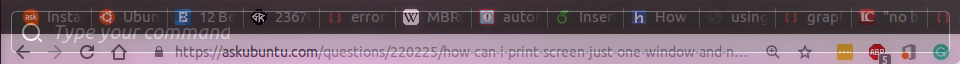
\includegraphics[width=0.8\textwidth]{hello-c-with-gvim.jpg}

\includegraphics[width=0.8\textwidth]{hello-c-with-gedit.jpg}
\end{center}
\כיתוב|עריכת קובץ המכיל תכנית \סי באמצעות העורך gvim|
\תגית|איור:וים|
\end{איור}

בין כך, ובין כך, לאחר שהקובץ נוצר, עלי להדר אותו. כדי להדר את הקובץ בסביבת
החישוב שלי, אכתוב:
\bash[script]
cc hello.c
\END

ואחר כך, כל שנותר לי לעשות כדי להריץ את התכנית, הוא לכתוב:
\bash[verbose,script,stdout]
./a.out
\END

עיניך הרואות, סדרת הפעולות הנדרשת בכדי ליצור את התכנית הפשוטה הזו, להדרה
ולהפעילה, עשוייה להיות מעט מורכבת. אבל, אין מנוס מכך: התנסות בלתי אמצעית
בפעולות אלו חיונית לשם רכישת יכולת שימוש בשפה.

מטבע הדברים, ספר זה לא יוכל להוות תחליף להתנסות האישית הזו בסביבת המחשוב
המיוחדת שלך. יהיה עליך לעשות זאת בעצמך, ולחזור ולעשות זאת מחדש בעבור כל שפת
תכנות שתלמד, ובעבור כל סביבת מחשב עליה תבחר לעבוד.

אולם, עצם ההסתכלות בתכנית "שָׁלוֹם, עוֹלָם!" ובתכניות אחרות, קצרות ככל שתהיינה,
יכולה ללמד את המעיין רבות על השפה בה הן כתובות, על הדקדוק שלה, ואולי על כמה
עקרונות בתכנון שלה. בפרק זה נכיר כמה כלים שיסייעו לנו בלימוד הזה, ונאמן את
עיננו לבחון תכניות, במיוחד תכניות הכתובות בשפת תכנות שאינה מוכרת לנו, לעומקן.

ראשית, נאתר את המרכיבים הדקדוקיים היסודיים, ונראה שאלו מופיעים שוב ושוב בשפות
תכנות שונות. אחר כך, נגלה שבתכנון דקדוק בעבור שפות תכנות שונות, יש שאלות
מסויימות אשר חוזרות על עצמן שוב ושוב.

כך למשל, הגדרת כל שפת תכנות חייבת להתמודד עם הצורך לצייד את המתכנת במנגנון
לכתיבת \הערות. אנו נראה כי אף הפתרונות בהם בוחרים מתכנני השפות בעבור בעיות אלו
נוטים לחזור על עצמם. ובאמת, מספר הדרכים השונות שבהן ניתן לכתוב \הערות בשפות
תכנות שונות אינו רב.

הכרה של השאלות הללו---צמתי ההחלטה בזמן תכנון השפה, ומרחב הפתרונות המוכרים
לשאלות, יסייעו לנו לזהות בקלות, מתוך הצצה חטופה לפעמים, בפתרון בו בחר מתכנן
השפה.

§ מרכיבים דקדוקיים יסודיים
מקובל להציג תכניות באופן המבליט את תפקידם השונה של המרכיבים הדקדוקיים היסודיים
בשפה. הנה למשל, אם נסתכל ב\עע איור וים נראה שהעורך gvim משתמש בצבעים שונים לשם
הצגת הקובץ \קד{hello.c}.

סביר שה\עורך או סביבת הפיתוח האינטראקטיבית שלך אף הם משתמשים בהבלטה ויזואלית
מעין זו המודגמת באיור. למעשה, הבלטה ויזואלית של מרכיבים דקדוקיים שונים היא כה
נפוצה, עד שישנן \ספריות תכנה המשרתות צורך זה.

ב\לינוקס למשל, ישנה \ספריה בשם gtksourceview התומכת בהבלטה דקדוקית של שפות
שונות. התקנה רגילה של gtksourceview תומכת ביותר משבעים שפות תכנות. היכולת
לתמוך במספר כה רב של שפות מוסברת בכך שרשימת המרכיבים היסודיים השונים אינה
ארוכה, והיא בדרך כלל מכילה שישה סוגים עיקריים:
\begin{ספרור}
✦ \מילולונים מסוג של מספר שלם, מספר ממשי, תו ו\סדרית.
✦ \הערות
✦ \מונח[מילה שמורה]{מילים שמורות}
✦ \מזהים
✦ סימני פעולה שונים, כגון אופרטורים מתימטיים והצבה.
✦ סימני פיסוק שונים, המסייעים לקורא ול\מהדר לזהות את חלקי התכנית השונים.
\end{ספרור}
שלושת הסוגים הראשונים הם אלו הזוכים בדרך כלל להבלטה ויזואלית ייחודית. אף בספר
זה נשתמש ב\מוסכמות ויזואליות להבלטת המרכיבים הדקדוקיים היסודיים. \עע תכנית
שלום:סי מציגה שוב את התכנית \קד{hello.c} שכתבתי תוך שימוש ב\מוסכמות אלו.

\begin{תכנית}
\setLTR
\lstinputlisting[language=C++,style=Numbered]{00/hello.c}
\setRTL
\כיתוב|"שָׁלוֹם, עוֹלָם!" בשפת \סי|
\תגית|תכנית:שלום:סי|
\end{תכנית}

\מוסכמות אלו תשמשנה גם בעבור שפות תכנות אחרות. הנה נכתוב למשל תכנית "שָׁלוֹם,
עוֹלָם!" בשפת פסקל.

\begin{קוד}
\bash[verbose,script]
rm -f hello.p; cat << EOF > hello.p
{hello.p: My very first Pascal program. It does not do
  too much---it prints the string "Hello, World!" (followed
by a new line), and then terminates.}

program HelloWorld(output);
begin
  WriteLn('Hello, World!')
end.
EOF
\END
\end{קוד}

גם את תכנית זו אהדר, כדי לבדוק שלא שגיתי
\bash[script,stdout,ignoreStderr]
pc hello.p
\END
וכמובן, אריץ את התכנית, בכדי לבדוק שהיא אכן עושה את אשר עליה לעשות.
\bash[script,stdout]
./a.out
\END

כעת, \עע תכנית שלום:פסקל מציגה את תכנית הפסקל שכתבתי תוך שימוש ב\מוסכמות שלנו.

\begin{תכנית}
\setLTR
\lstinputlisting[language=Pascalx,style=Numbered]{00/hello.p}
\setRTL
\כיתוב|"שָׁלוֹם, עוֹלָם!" בשפת פסקל|
\תגית|תכנית:שלום:פסקל|
\end{תכנית}
כפי שניתן לראות הן ב\עע תכנית שלום:סי והן ב\עע תכנית שלום:פסקל, אנו נוהגים
לכתוב תכניות ב\מונח{גופן ברוחב קבוע}. \מונח[מילה שמורה]{המילים השמורות} בתכנית
מודגשות בכך שהן כתובות בגופן עבה מעט יותר, המילולונים מסוג סדריות כתובות בגופן
שבו האותיות נטויות, וה\הערות מופיעות בכתב מסולסל וב\מונח{גופן יחסי}.

בעיון ב\עע תכנית שלום:סי אנו יכולים לזהות שלוש \מונח[מילה שמורה]{מילים שמורות}
בשפת \סי: \מש{int}, \מש{char} וְ-\מש{return}. 
לעומת זאת, ההוראה 
\LR{\cpp{#include}}
אינה מילה שמורה, וכפי שנווכח בהמשך, עד כמה שהדבר מבלבל, שורה 6 כולה אינה כתובה
בעצם בשפת \סי.

בעיון ב\עע תכנית שלום:פסקל אנו יכולים לזהות שלוש \מונח[מילה שמורה]{מילים
  שמורות} בשפת פסקל: המילה \מש{program} המציינת את תחילת התכנית, המילה
\מש{begin} המציינת את תחילת ה\פקודות לביצוע, והמילה \מש{end} המציינת את סוף
רשימת ה\פקודות לביצוע.

קל גם לזהות את המרכיבים הדקדוקיים היסודיים האחרים בשתי התכניות שהצגנו. בשפת
\סי אנו רואים הערה אחת (המשתרעת על שורות 1-4 ב\עע תכנית שלום:סי), שני \מזהים
(המילה \קד{main} והמילה \קד{printf}), את המילולון מסוג \סדרית (בשורה 10), את
ה\מילולון מסוג מספר שלם (המספר \קד{0} בשורה 11) וכן שמונה סימני פיסוק שונים:

\begin{english}
\let\ttfamily=\listingsfont
\begin{CPP}
  () { } [ ] ; *
\end{CPP}
\end{english}

ב\עע תכנית שלום:פסקל אנו רואים הערה אחת (בשורה 1), שלושה \מזהים (המילים
\קד{HelloWorld}, \קד{output} וְ-\קד{WriteLn}) ואת ארבעת סימני הפיסוק הבאים:


§ אוצר המילים
בהסבר לעיל של תָּכְנָן של שתי תכניות "שָׁלוֹם, עוֹלָם!" שכתבתי, השתמשתי במונחים
\מונח[מילה שמורה]{מילים שמורות} ו\מזהים. המונחים הללו מוכרים
ודאי לכל מי שכתב תכנית מחשב,
ובכל זאת, כדאי להזכיר את משמעותם, ולדון באופן שבו מוגדר אוצר המילים של שפת
התכנות. אחר כך, נבחין בין סוגי ה\מזהים השונים, ובהם
\מונח[מזהה שמור]{מזהים שמורים},
\מונח[מזהים מוגדרים מראש]{מזהים המוגדרים מראש}, \מונח{מזהי ספריה}, ו\מזהים סתם.

§§ הצורך במזהים
כידוע, תכנית מחשב מתארת תהליך חישובי, והתיאור נעשה כמעט תמיד באורח מודולארי.
שפת התכנות מציעה למשתמש בה אוסף של פעולות חישוביות יסודיות, פעולות הבנויות
בשפה. המתכנת מגדיר סדרות של פעולות חישוביות כאלו, מעניק להן שמות, ומשתמש
בשמות הללו כדי לבנות סדרות מורכבות יותר המכילות אותן.

כך למשל בשפת \סי, המתכנת מגדיר פונקציות, נותן לפונקציות הללו שמות, ואחר כך
משתמש בשמות אשר ניתנו לפונקציות, כדי לפנות אליהן מפונקציות אחרות, ובכך להגדיר
פונקציות מורכבות יותר.

לא רק לפונקציות יש שמות. ניתן לתת שמות ל\משתנים, ל\קבועים,
ל\טיפוסים, ול\ישויות
אחרות המופיעות בתכנית. שם של \ישות כזו נקרא \מזהה.
ו\מזהה כשמו כן הוא: הוא \מזהה \ישות ומאפשר לפנות אליה אחרי
שנוצרה.

§§ הגדרת מזהה חוקי

הדקדוק של שפת התכנות מכיל כללים המגדירים מהו \מזהה חוקי.
כך למשל, בשפת \סי, \מזהה הוא:

\begin{מובאה}
סדרה של תוים היכולים להיות אות לטינית גדולה, \קד{A-Z},
אות לטינית קטנה \קד{a-z}, ספרה \קד{0-9} או
\מונח[תו קו תחתון]{תו הקו התחתון}
\קד{\_},
ובלבד שסדרה זו אינה מתחילה בספרה.
\end{מובאה}

המילים \קד{main} וְ-\קד{printf} שראינו ב\עע תכנית שלום:סי, עומדות בכללים אלו,
ועל כן בקהל ה\מזהים הן תחשבנה.

הכללים הקובעים אם סדרת תוים היא \מזהה אם לאו דומים מאוד בכל השפות,
ובדרך כלל, ניתן להניח כי הגדרת שם מזהה בשפה לא מוכרת היא כמו זו של שפת \סי.

כרגיל, ישנם יוצאים מן הכלל, העשויים אפילו להרגיז: בשפת המקרו של
\LR{\TeX}.

 מזהה יכול להכיל אותיות בלבד, ובגירסאות מוקדמות של שפת בייסיק, מזהה יכול היה
 להיות בן אות אחת בלבד, או אות בודדת אחריה מופיעה ספרה אחת.%
\הערת␣שוליים{מגבלות
  קיצוניות על אורך מזהה היו נפוצות בעבר: בגירסאות מוקדמות של שפת פורטרן, אורכו של
  מזהה הוגבל לשישה תוים בלבד, ובגירסאות מוקדמות של שפת \סי, אורך מזהה הוגבל
  לשמונה תוים. מגבלות כאלו כמעט שאינן קיימות בשפות חדשות או בגרסאות עדכניות של
שפות ותיקות.}

לבד מחריגים אלו, יש כמה הבדלים עקרוניים בין שפות התכנות, אליהם כדאי לשים לב.

§§ אבחנה בין אותיות גדולות וקטנות

ראשית, ישנן שפות אשר אינן מבחינות בין אותיות גדולות וקטנות, בשפות אלו, אין כל
הבחנה בין המזהים \קד{HELLO}, \קד{Hello}, וְ-\קד{hello}. הסיבה לתכנון כזה של
השפה, יכולה להיות היסטורית (שפת פסקל פותחה על מחשבים שבהם אוסף התוים לא הבדיל
בין אותיות גדולות וקטנות), או עקרונית, אם לדעת מתכנן השפה, האבחנה בין אותיות
קטנות וגדולות, הינה מבלבלת או מיותרת.

בשפות רבות, ישנן \מוסכמות ביחס לשימוש באותיות גדולות וקטנות בעבור \מזהים מסוגים
שונים. בשפת \גאוה למשל, מקובל לכנות \מחלקה בשם המתחיל באות גדולה, לתת ל\קבועים
שמות המורכבים מאותיות גדולות בלבד, ולהשתמש בשם המתחיל באות קטנה בעבור
כל ה\ישויות האחרות, כולל פונקציות ו\משתנים.

ה\מהדר אינו אוכף את ה\מוסכמות הללו, ותכנית שאינה מצייתת
ל\מוסכמות, היא עדיין תכנית חוקית. בכל זאת, יש חשיבות ל\מוסכמות
הללו, בכך שהן מקלות על כתיבת התכנית: כאשר כתבתי את
\עע תכנית שלום:גאוה, לא הייתי צריך להתלבט אם לכנות את
ה\מחלקה \קד{HELLO}, או \קד{hello}. פעלתי באורח מוכני
לפי ה\מוסכמות, והשתמשתי ב\מזהה{Hello} ל\מחלקה.

שימוש ב\מוסכמות מקל גם על הקורא. כאשר בתכנית \גאוה מופיעה
ה\פקודה
\begin{קוד}
\begin{Pascal}
foo.bar();
\end{Pascal}
\end{קוד}


קל לנחש כי המזהה \קד{foo} מתייחס ל\משתנה, אשר עליו מופעלת הפונקציה
\שי{\קד{bar()}}. לעומת זאת, הכתיב

\begin{קוד}
\begin{Pascal}
Foo.bar();
\end{Pascal}
\end{קוד}

רומז כי מדובר ב\מחלקה אשר שמה הוא \קד{Foo}, וכי המזהה \קד{bar}
מתייחס לפונקציה \סטאטית המוגדרת בתוכה.

צריך לשים לב כי ה\מוסכמות הללו עשויות להשתנו בין שפה לשפה.
בשפת אייפל למשל, מקובל כי ה\מזהה של מחלקה נכתב כולו באותיות
גדולות, ובשפת \שי{\CSharp} מקובל דווקא לתת לפונקציות שמות המתחילים באות גדולה.

§§ הגבלת מזהים לישויות מסוג מסויים
בשפות מסויימות, המבנה הדקדוקי של ה\מזהה קובע בעבור מה ניתן להשתמש בו. בשפת
פרולוג לדוגמא, שם של \משתנה חייב להתחיל באות גדולה או ב\מונח[תו קו תחתון]{תו
הקו התחתון}.

בשפות אחרות, המבנה הדקדוקי של ה\מזהה עשוי לקבוע את טיבו של הפריט המזוהה. כך
למשל בשפת פורטרן, טיפוסו של \משתנה אשר שמו מתחיל באות-I הוא מספר שלם, ואילו
הטיפוס של \משתנה אשר שמו מתחיל באות-X הוא מספר ממשי.

הכתבה דומה קיימת גם בשפת פרל, שם \מזהה המתחיל בסימן \קד{\$} יכול להתייחס רק
למשתנה סקלארי, \מזהה המתחיל בסימן \קד{\@} יכול להתייחס רק למערך, \מזהה המתחיל
בתו \קד{%} יכול להתייחס רק לטבלת ערבול, ואילו \מזהה המתחיל באות מאותיות
האלפבית הלטיני, יכול להתייחס אך ורק לפונקציה.

§§ מזהה הבנוי מהלחם של כמה מילים
תכנון שפת תכנות מנסה לתת מענה גם לצורך של מתכנתים לתת לישויות שמות אשר יבטאו
את תָּכְנָן. זו הסיבה ששפות מודרניות נִתְּצוּ את שלשלאות ה-ASCII והן מתירות שימוש
בתוי יוניקוד. מזהים בשפות כאלו יכולים להכיל אותיות הלקוחות מכל אלפבית שהוא.
בתכנות של אלגוריתם מתימטי, השם~$Γ$ הוא שם סביר ביותר לפונקציה.

קושי מהותי יותר במתן שמות משמעותיים
הוא העובדה שלעיתים נדרשת יותר מאשר מילה אחת
כדי לבטא נכונה את מהותה של ישות. אמנם \מזהים כמו \קד{fileopen}
הם לגיטימיים, אך בכל זאת, קל הרבה יותר לזהות את שתי המילים שהולחמו לכדי \מזהה
אחד אם שמו יהיה \קד{file\_open}.

אכן, מקובל להשתמש בקו התחתון להפריד בין שתי מילים מולחמות, וזו כנראה אחת
הסיבות החשובות שניתן היתר להשתמש בתו הקו התחתון במזהים. \מוסכמה מקובלת אחרת
היא להשתמש במה שקוראים \הדגש{camelCase} כדי להפריד ויזואלית בין מילים מולחמות.
לפי \מוסכמה זו, כל מילה מולחמת, לבד מהמילה הראשונה, תתחיל באות גדולה. כך,
נכתוב \קד{fileOpen} כדי לציין את ה\מזהה שמורכב מהלחם של המילה {file} עם המילה
\שי{open}.

כזכור, שפת פסקל אינה מבחינה בין אותיות גדולות וקטנות. כאשר כתבתי
\מוגדרת␣מראש{WriteLn} בשורה מס'~7 ב\עע תכנית שלום:פסקל, השתמשתי ב\מוסכמה הידועה
בשם \הדגש{PascalCase} כדי להפריד בין המילה {write} ובין המילה \שי{ln} (שהיא
קיצור למילה \שי{line}), כדי להציג את ה\מזהה הזה. ב-{PascalCase} כל המילים
המולחמות מתחילות באות גדולה. (שים לב לכך שכיוון שפסקל אינה מבחינה בין אותיות
גדולות וקטנות יכולתי לכתוב \מוגדרת␣מראש{writeln} או \מוגדרת␣מראש{WRITELN} מבלי
לשנות מהתכנית כלל.)

בשפת קובול, תו המקף (\קד{-}), המשמש בדרך כלל לציון פעולת החיסור יכול להופיע
במזהה. ב\עע תכנית שלום:קובול ("שָׁלוֹם, עוֹלָם!" בשפת קובול), אנו רואים מספר לא קטן
של \מזהים המכילים בתוכם מקף.

\begin{תכנית}
\setLTR
\lstset{comment=[f][commentstyle][1]*}
\begin{COBOL}
IDENTIFICATION DIVISION.
PROGRAM-ID. HELLO-WORLD.

*** Hello, World! in the COBOL programming language

ENVIRONMENT DIVISION.
CONFIGURATION SECTION.
SOURCE-COMPUTER. RM-COBOL.
OBJECT-COMPUTER. RM-COBOL.

DATA DIVISION.
FILE SECTION.

PROCEDURE DIVISION.

MAIN-LOGIC SECTION.
BEGIN.
DISPLAY " " LINE 1 POSITION 1 ERASE EOS.
DISPLAY 'Hello, World!' LINE 15 POSITION 10.
STOP RUN.
MAIN-LOGIC-EXIT.
EXIT.
\end{COBOL}
\כיתוב|"שָׁלוֹם, עוֹלָם!" בשפת קובול|
\תגית|תכנית:שלום:קובול|
\end{תכנית}

שפת אלגול 68, כמו גם שפת פורטרן מתעלמת מרווחים המופיעים בתוך \מזהים, דבר המאפשר
להפריד בין מילים מולחמות באמצעות רווחים.

§ מילים שמורות וסוגי מזהים

\מונח[מילה שמורה]{המילים השמורות} הינן מילים אשר למרות שהן עומדות בכללים
הקובעים מהו \מזהה, הן שמורות למטרות אחרות, ולא ניתן להשתמש בהן לשם מתן שם
ל\ישויות אשר נוצרו על ידי המתכנת. כך למשל המילה \מש{int} בשפת \סי עומדת בכללים
המגדירים \מזהה חוקי בשפה, אך היא אינה \מזהה. לא ניתן לכתוב פונקציה בשפת \סי
אשר שמה הוא \מש{int}.

§§ קבוצות מוגדרות רקורסיבית
לאילו צרכים משמשות אם כן \מונח[מילה שמורה]{המילים השמורות}? במקרים
רבים, \מונח[מילה שמורה]{המילים השמורות} משמשות כעין סימני פיסוק. המילים
\מש{program}, \מש{begin} וְ-\מש{end} בשפת פסקל הן בבירור כאלו. יש עוד שימושים
רבים אחרים למילים השמורות, ואין זה המקום למנות את כל אלו. כאן אנו נתמקד בשימוש
אחד חשוב של \מונח[מילה שמורה]{מילים שמורות}. לעיתים, \מונח[מילה שמורה]{מילים
שמורות} משמשות לזיהוי \ישויות "אטומיות". כדי להבין את המונח \ישות אטומית,
נזדקק להגדרה הבאה:

נאמר על קבוצה כי היא \מונח[קבוצה מוגדרת רקורסיבית]{מוגדרת רקורסיבית}
אם הגדרת הקבוצה בנויה על פי התבנית הבאה:
\begin{ספרור}
✦ רשימה, בדרך כלל סופית וקצרה של ערכים יסודיים.
✦ מנגנון או מנגנונים לבניה של ערכים מורכבים מהערכים היסודיים
וערכים מורכבים אחרים.
\end{ספרור}

כך לדוגמא, קבוצת ה\ביטויים היכולים להפיע בשפת תכנות כגון שפת פסקל, היא קבוצה
המוגדרת רקורסיבית: ה\ביטויים היסודיים הם מילולונים וקריאת ערכם של \משתנים.
ביטויים מורכבים נוצרים מביטויים אחרים, היכולים להיות ביטויים יסודיים, או
ביטויים מורכבים אחרים, באמצעות מגוון של פעולות, הכוללות, בין השאר, את פעולות
החשבון וקריאות לפונקציה.

\ישות מקבוצה המוגדרת רקורסיבית היא \ישות אטומית אם לא ניתן לזהות בתוכה
תת-\ישות השייכת לאותה קבוצה. חשוב להבין כי \ישות אטומית אינה בהכרח לא פריקה,
כל שנדרש הוא שלא ניתן לזהות בתוכה תת-\ישות מאותה קבוצה. הנה, קבוצת הפקודות
במרבית שפת תכנות היא קבוצה המוגדרת רקורסיבית, ובתוך קבוצה זו, אנו יכולים לזהות
את הפקודות האטומיות. בשפת פסקל, \הצבה היא \פקודה אטומית. אבל, אם נעיין ב\פקודה
\begin{קוד}
\pascal{a :=b+c;}
\end{קוד}
שהיא \פקודה אטומית, נוכל לזהות בה תתי מרכיבים, למשל הביטוי \קד{b+c}. בכל זאת,
הפקודה לעיל היא פקודה פרימטיבית, שכן לא ניתן לזהות בה תת-מרכיב שהוא
\פקודה בעצמו.

לעומת זאת, ה\פקודה הבאה בפסקל,
\begin{קוד}
\begin{PASCAL}
begin
  a :=b+c;
end
\end{PASCAL}
\end{קוד}
אינה פקודה אטומית, שכן ניתן לאתר בה מרכיב שהוא \פקודה בעצמו.

קבוצת ה\טיפוסים של שפת \סי (כמו גם קבוצת הטיפוסים של שפת פסקל) אף היא קבוצה
המוגדרת רקורסיבית: ישנם טיפוסים מורכבים, אשר ניתן לזהות כי הם מורכבים מיחידות
קטנות יותר, אשר אף הן טיפוסים. בטיפוס רשומה למשל ניתן לזהות כיחידות
קטנות יותר את טיפוסי השדות הבונים את הרשומה. אנו אומרים שהטיפוס של רשומה
הוא \מונח{טיפוס מורכב}, משום שיש בו תתי-יחידות אשר אף הן טיפוסים.

לעומת ה\מונח[טיפוס מורכב]{טיפוסים המורכבים}, ישנם טיפוסים אטומיים, כלומר
טיפוסים אשר לא ניתן לזהות בתוכם טיפוסים אחרים. הטיפוס של מספרים שלמים או
הטיפוס של מספרים ממשיים, הם דוגמאות לטיפוסים כאלו.

המילה השמורה \מש{int} בשפת \סי \מזהה את הטיפוס האטומי של מספר שלם.
מילים
שמורות המשמשות כ\מזהים נקראות \מונח{מזהה שמור}.

שפת פסקל נוקטת בשיטה אחרת במקצת לזיהוי הטיפוסים האטומיים. המילה
\מוגדרת␣מראש{Integer} אשר מתארת את הטיפוס האטומי של מספרים שלמים בשפת
פסקל אינה מילה שמורה. אלא היא מילה \הדגש{מוגדרת מראש}. המונח מילה מוגדרת
מראש, מכוונת לכך שאף בתכנית פסקל ריקה, קיימת הגדרה הקושרת את
ה\מזהה{} \מוגדרת␣מראש{Integer} אל הטיפוס האטומי של מספרים שלמים. עלינו להבחין בין
הטיפוס, ובין שמו: אין למתכנת גישה לטיפוס האטומי הזה עצמו---אין באפשרותו לבחון
אותו, או לנסות לפרק אותו למרכיבים. אלא, שבניגוד למילים שמורות, ישנה האפשרות
למתכנת להשתמש בשמו של הטיפוס \מוגדרת␣מראש{Integer} מחדש לצרכים אחרים לפי
בחירתו, כלומר לקשור את ה\מזהה הזה לשפה אחרת.

גם קבוצת הפעולות החישוביות היא קבוצה המוגדרת רקורסיבית. ישנן פעולות חישוביות
אטומיות של שפת התכנות, כאלו שאי אפשר לחלק אותן לתתי-יחידות שאף הן פעולות
חישוביות, וכנגדן ישנן הפעולות החישוביות המורכבות, כגון פונקציה בשפת \סי.

מקצת הפעולות החישוביות האטומיות בשפת \סי ופסקל מסומנות בסימני פעולה, הכוללים
בין היתר אופרטורים מתימטיים שונים. ישנן גם פעולות חישוביות אטומיות אשר להן
הוקדשה מילה שמורה. ה\פקודה
\begin{קוד}
\cpp{return 0;}
\end{קוד}
אשר בשורה 11 ב\עע תכנית שלום:סי, עושה שימוש במילה שמורה כזו.

ישנן שפות, כמו קובול, המקד\ישות מספר רב של \מונח[מילה שמורה]{מילים שמורות}
לפעולות החישוביות האטומיות. בין השאר, יש בקובול \מונח[מילה שמורה]{מילים
שמורות} יחודיות בעבור חיבור, חיסור, כפל וחילוק.

§§ מזהים שמורים לשגרות
על אף העובדה שקבוצת הפעולות החישוביות מוגדרת רקורסיבית, אין די בחלוקה לפעולות
מורכבות ולפעולות אטומיות. ישנן פעולות חישוביות רבות אשר על אף שאינן אטומיות,
מתכנת רגיל לא ירצה לבנותן בעצמו. הדוגמא הראשית לסוג כזה של פעולות הן פעולות של
הוצאת פלט וקבלת קלט.

ישנן שפות בהן פעולות של קלט ופלט בנויות לתוך השפה, והגישה אליהן נעשית באמצעות
\מזהים שמורים. כזהו המצב בשפת \AWK, כמודגם ב\עע תכנית שלום:AWK.

\bash
cat << EOF > hello.awk
#!/usr/bin/gawk -f
BEGIN { # "Hello, World!" in the AWK programming language
  print("Hello, World!")
  exit
}
EOF
chmod +x hello.awk
./hello.awk
\END
\begin{תכנית}
\setLTR
\lstinputlisting[language=AWK,style=Numbered]{00/hello.awk}
\setRTL
\כיתוב|"שָׁלוֹם, עוֹלָם!" בשפת AWK|
\תגית|תכנית:שלום:AWK|
\end{תכנית}
המילה \מש{print} המופיעה בשורה מס'~8 בתכנית היא מילה שמורה. כלומר, נאסר על
המתכנת להשתמש בשם זה בעבור \ישויות אחרות בתכנית, והגדרת משמעותה של הפונקציה
\מש{print} היא חלק מהגדרת שפת \שי{AWK}.

§§ מזהים מוגדרים מראש
האופן שבו מאפשרת שפת פסקל שימוש בפעולות של קלט ופלט היא מעט שונה מזו הנוהגת
בשפת \שי{AWK}. במקום \מונח[מילה שמורה]{מילים שמורות}, שמן של פעולות הקלט והפלט
הוא \מזהים המוגדרים מראש. ה\שגרה \מוגדרת␣מראש{WriteLn} אשר נקראה בשורה 4 של
\עע תכנית שלום:פסקל, היא בדיוק כזו. זוהי \שגרה הבנויה בשפת התכנות פסקל, ואשר
למתכנת אין גישה אליה. כלומר, המתכנת אינו יכול לבחון את אופן המימוש של ה\שגרה,
והוא אף אינו יכול לממש מחדש באופן אחר את ה\שגרה הזו. יתירה מזאת, משמעותה של
ה\שגרה היא חלק בלתי נפרד מהגדרת שפת פסקל.

בכל זאת, המילה \מוגדרת␣מראש{WriteLn} אינה \מונח{מילה שמורה}. המילה אמנם \מזהה
\שגרה הבנויה בשפה, אך הרשות מסורה בידי המתכנת לקשור שם זה ל\ישות אחרת.

ב\עע תכנית שלום:פסקל נצבעו המזהים המוגדרים מראש בצבע כחול. אנו רואים שגם המילה
\מוגדרת␣מראש{output} צבועה בצבע זה. מילה זו אף היא מהווה \מזהה מוגדר מראש, אך
אנו לא נעמיק בו.

כיצד מוממשה ה\שגרה{} \מוגדרת␣מראש{WriteLn} בפסקל? כיצד מומשה הפונקציה
\קד{printf} בשפת \סי? מסתבר כי על אף שמדובר בפעולות חישוביות מורכבות, אי אפשר
    לממש אותן רק באמצעות הפעולות החישוביות האטומיות שבשפה. שפת פסקל אינה מגלה
    למשתמש בה כיצד נסגר הפער הזה. לעומת זאת, ההגדרה של שפת \סי, מכילה "דלת אחורית"
    שבאמצעותה אפשר לממש את \קד{printf}. מהותה של דלת אחורית זו היא הן היכולת להפעיל
    מתוך שפת \סי \פקודות חישוביות בשפת מכונה, והן היכולת לקרוא משפת \סי ישירות
    לשירותים של מערכת ההפעלה. הגדרתה של שפת פסקל אינה חושפת בפני
    המשתמש דלת אחורית כזו---כל הפעולות אותן יכול המתכנת לעשות בשפת פסקל
    מוגדרות כחלק מהגדרת השפה עצמה. אך כמובן, המימוש של \מוגדרת␣מראש{WriteLn} (אשר אינו
    חשוף למשתמש בשפה) חייב להשתמש במנגנונים המצויים מחוץ לשפה עצמה.

    האופן שבו שפת \סי תומכת בפעולות קלט ופלט שונה מהותית מזו של שפת פסקל. הפונקציה
    \קד{printf} אשר נקראה בשורה 11 של \עע תכנית שלום:סי, הוגדרה בספריה. הספריה היא
    אמנם סטנדרטית, במובן זה שבדרך כלל כל תכנית \סי שתכתוב תוכל לקרוא לה. אולם,
    הספריה ניתנת להחלפה, והרשות נתונה בידי המתכנת לממש אותה מחדש.

    §§ סיכום: סוגי מזהים
    \עע טבלא מזהים מסכמת את ההבדלים בין הסוגים השונים של המזהים: \מזהים שמורים הם
    התקיפים ביותר: הם זמינים תמיד, לא ניתן למתכנת לבחון את מימושם, נאסר עליו לשנות
    את המימוש, ונאסר עליו להשתמש במזהים אלו לצורך אחר. חלשים מעט מאלו הם המזהים
    המוגדרים מראש, אשר הותר למתכנת לקשור אותם למימוש אחר. מזהי ספריה הם החלשים
    ביותר: אמנם הם זמינים תמיד, אך המתכנת יכול לבחון את המימוש שלהם ולשנותו, וכן
    להשתמש בהם לצרכים אחרים.

    \begin{טבלא}[!htbp]
    \begin{center}
    \renewcommand\codesize\footnotesize
    \footnotesize
    \begin{tabular}{|r||r|p{16ex}|p{16ex}|p{16ex}|}
    \hline
    סוג & דוגמא & שם מוגן מפני שימושים נוספים
    & מימוש חשוף למתכנת ובר שינוי על ידו
    & מובנה בסביבת העבודה
⏎ \hline
    \מזהה שמור & \מש{print} בשפת AWK & כן & לא & כן ⏎
    \מזהה מוגדר מראש &
    \begingroup\color{blue}\קד{WriteLn}\endgroup{}
    בשפת פסקל & לא & לא & כן ⏎
    \מזהה ספריה & \קד{printf} בשפת \סי & לא & כן & כן ⏎
    \מזהה אחר & \קד{HelloWorld} ב\עע תכנית שלום:פסקל & לא & כן & לא ⏎
    \hline
    \end{tabular}
    \end{center}
    \כיתוב|סוגי מזהים בשפות תכנות|
    \תגית|טבלא:מזהים|
    \end{טבלא}

    הנטיה המודרנית היא להשתמש ככל שניתן במזהי ספריה בעבור פעולות קלט פלט
    ודומותיהן, ולמעט בשימוש במזהים מוגדרים מראש ובמזהים שמורים. הסיבה היא שמימוש
    העשוי במסגרת השפה מסבך את הגדרת השפה שלא לצורך וכובל אותה מפני שינויים בעתיד.
    בשפת \סי למשל, אין \מזהים מוגדרים מראש כלל.

    הנטיה המודרנית התרחקה גם מהגישה של שפת פסקל להגדיר טיפוסים אטומיים באמצעות
    \מזהים מוגדרים מראש, אולם מפאת הקושי להגדיר טיפוסים אטומיים באמצעות ספריה, אף
    אם לזו יש גישה לשפת מכונה, בשפות מודרניות טיפוסים אטומיים מוצעים למתכנת בדרך
    כלל באמצעות \מזהים שמורים.

    הבה ונבחן את \עע תכנית שלום:Go, תכנית "שָׁלוֹם, עוֹלָם!" בשפת \Go, באמצעות המונחים
    שהכרנו.

\begin{תכנית}
\begin{GOn}
// "Hello, World!" in the Go programming language
package main
import "fmt"
func main() {
  fmt.Printf("Hello, World!\n")
}
\end{GOn}
\כיתוב|"שָׁלוֹם, עוֹלָם!" בשפת Go|
\תגית|תכנית:שלום:Go|
\end{תכנית}

אף מבלי להכיר את שפת \שי{Go}, קל להסיק שהמילים השמורות שבשפה אשר מופיעות
בתכנית, \מש{package}, \מש{import}, וְ-\מש{func}, אינן בבחינת \מזהים, משום שהן
אינן נוקבות בשמה של \ישות תכנותית.

לעומתן, שם הפונקציה \קד{Printf} אשר אחראית להצגת ה\סדרית, היא \מזהה ספריה.

§ יבוא מזהים מהספריה
אם הספריה הסטנדרטית של שפת התכנות אינה חלק משפת התכנות עצמה, הרי אפשר להחליף
את הספריה הזו בספריה אחרת. כך למשל, אפשר לכתוב ספריה חליפית בעבור שפת \סי בה
הפונקציה המציגה סדריות נקראת למשל \קד{typeoupt}. אם נעשה כן, יהיה צורך כמובן
לכתוב את \עע תכנית שלום:סי מעט אחרת.

בכל שפה המשתמשת במזהי ספריה, נדרשת אם כן דרך להודיע ל\מהדר מהם המזהים המצויים
בספריה. בדיקה בעין בוחנת של התכנית "שָׁלוֹם, עוֹלָם!" בשפה המשתמשת במזהי ספריה תגלה
את האופן שבו הדבר נעשה.

§§ יבוא באמצעות מילה שמורה
ב\עע תכנית שלום:Go הכתובה בשפת \Go היבוא של \מזהים מהספריה נעשה באמצעות ההוראה
\begin{קוד}
\go{import "fmt"}
\end{קוד}
המצוייה בשורה מס'~3, ובה מילה שמורה של השפה אחראית ל\יבוא ה\מזהה.

נשים לב לכך שהפונקציה \קד{Printf} מצוייה בתוך חבילה אשר שמה \קד{fmt} וכי
ההוראה
\begin{קוד}
\go{import "fmt"}
\end{קוד}
מייבאת את החבילה כולה.

נשים לב גם לכך שהקריאה לפונקציה \קד{Printf} מציינת שהיא נלקחת מתוך
החבילה \קד{fmt}, ככתוב בשורה מס'~5 ב\עע תכנית שלום:Go{:}
\begin{קוד}
\lstset{language=Golang}
\lstinline+fmt.Printf("Hello, World!\n")+
\end{קוד}

גם שפת עָדָה משתמשת במזהי ספריה. עיון בתכנית "שָׁלוֹם, עוֹלָם!" הכתובה בשפה זו (\עע
תכנית שלום:עָדָה), מגלה מבנה זהה כמעט לחלוטין לזה של שפת \Go, אם כי המילים הן
אחרות.

\begin{תכנית}

\begin{ADAn}
--Hello, World! in the Ada programming language
  with Text_IO;
  procedure Hello_World is
  begin
  Text_IO.Put_Line("Hello, World!");
  end Hello_World;
\end{ADAn}
\כיתוב|"שָׁלוֹם, עוֹלָם!" בשפת עָדָה|
\תגית|תכנית:שלום:עָדָה|
\end{תכנית}

שם פעולת הפלט בשפת עָדָה הוא \קד{Put\_Line}, והיא מצוייה בחבילה אשר שמה הוא
\קד{Text\_IO}. ההוראה

\begin{קוד}
\ada{with Text_IO;}
\end{קוד}
(שורה מס'~2 בתכנית) אף היא משתמשת במילה שמורה של שפת עָדָה בכדי לייבא חבילה זו
    לתוך התכנית. זאת, ועוד, אף בשפת עָדָה, ההפעלה של \קד{Text\_IO} מציינת את החבילה
    המכילה:

\begin{קוד}
\begin{ADA}
Text_IO.Put_Line("Hello, World!");
\end{ADA}
\end{קוד}

§§ יבוא באמצעות עיבוד מקדים
בשפת \סי היבוא של מזהי הספריה נעשה באופן מעט אחר. ב\עע תכנית שלום:סי הכתובה
בשפת \סי אחראית על כך ההוראה
\begin{קוד}
%\lstinline[language=C++]/#include <stdio.h>/
\end{קוד}
הגיעה העת להסביר מדוע נאמר לעיל שהוראה זו אינה כתובה בשפת \סי. מודל ההידור של
שפת \סי הוא יחודי בכך שההידור מתבצע בשני שלבים: טרם ההידור עצמו, מופעלת על
הקובץ המכיל תכנית \סי תכנית עיבוד ראשוני הידועה בשם \מונח[מעבד מקדים]{המעבד
המקדים}. שורות בקובץ התכנית המתחילות בתו הסולמית \קד{#} הן הנחיות \מונח[מעבד
מקדים]{למעבד המקדים} לביצוע טרנספורמציות טכסטואליות שונות על הקובץ אותו הוא
קורא. רק בשלב שני, מועבר תוצאת הטרנספורמציות הללו כקלט ל\מהדר עצמו לשם ביצוע
ההידור.

%בפרט, ההוראה \lstinline/#include/ מורה \מונח[מעבד מקדים]{למעבד המקדים} להכניס את תכנו
של קובץ אחר לתוך הקובץ המקורי. על כן, ההוראה
\begin{קוד}
%\lstinline/#include <stdio.h>/
\end{קוד}
תוחלף על ידי המעבד המקדים בתוכנו של קובץ אשר שמו \קד{stdio.h}, ואשר אותו יחפש
המעבד המקדים במקומות שונים במערכת הקבצים. תוכנו של קובץ זה מתאר את הפונקציה
\קד{printf} אשר בה משתמשת התכנית.

אמנם הפעלה של ה\מהדר תגרום מאחורי הקלעים להפעלה של \מונח[מעבד מקדים]{המעבד
  המקדים}, אך ניתן גם להפעיל את \מונח[מעבד מקדים]{המעבד המקדים} לבדו.
\bash[script,stdout]
cpp -P hello.c > hello.P.c
\END
הבה נשווה את גדלם של שני הקבצים:
\bash[script,stdout]
wc -l hello.c
\END
\bash[script,stdout]
wc -l hello.P.c
\END
אנו רואים שהקובץ לאחר \מונח[עיבוד מקדים]{העיבוד המקדים} גדול בהרבה מהקובץ
המקורי, ולכן לא נציג את כולו כאן. בכל זאת, ניתן לראות שאחרי העיבוד המקדים,
התווספה לתכנית שורה המגדירה את הפונקציה \קד{printf}
\bash[script,stdout]
grep -n "\<printf\>" hello.P.c
\END

ראינו אם כן שתי גישות ליבוא של מזהי הספריה אל התכנית המשתמשת בהן. בשפת \סי
היבוא נעשה באמצעות תהליך של \מונח{עיבוד מקדים} שהינו במובנים רבים בלתי תלוי
בתהליך ההידור עצמו. לעומת זאת, בשפות Go ועדה, היבוא נעשה באמצעות \מונח[מילה
שמורה]{מילים שמורות} של שפת התכנות.

§§ יבוא אוטומטי
לסיום הדיון בשאלת היבוא, נעייין ב\עע תכנית שלום:גאוה, תכנית "שָׁלוֹם, עוֹלָם!"
בשפת \גאוה. מסתבר שאף בשפה זו יש לבצע יבוא של מזהי הספריה, אלא, שבדיקתה של
\עע תכנית שלום:גאוה לא תגלה שם את פקודת היבוא.

\begin{תכנית}
\bash
cat << EOF > Hello.java
// Hello.java: my first Java program. It prints
// the string "Hello, World!" on the standard output
// stream, and then terminates.

class HelloWorld {¢¢
  static public void main(String args[]) {¢¢
    System.out.println("Hello, World!");
  }
}
EOF
\END
\setLTR
\lstinputlisting[language=Java,style=Numbered]{00/Hello.java}
\setRTL
\כיתוב|"שָׁלוֹם, עוֹלָם!" בשפת \גאוה|
\תגית|תכנית:שלום:גאוה|
\end{תכנית}

מתברר כי הגדרת השפה היא כזו ש\יבוא של חלקים נבחרים מהספריה נעשה באורח אוטומטי
    על ידי ה\מהדר. המתכנת אמנם רשאי לכתוב את פקודת ה\יבוא של חלקים אלו בעצמו,
    אך אין לו צורך לעשות כן. בין אם יעשה זאת ובין אם לאו, ה\מהדר ייבא את
    החלקים האמורים.

    § סביבת העבודה ונקודת התחלת הביצוע
    עיקרן של כל תכניות "שָׁלוֹם, עוֹלָם!" שראינו היה הוראה אחת להציג את ה\סדרית הזו.
    אנו נקרא להוראה חישובית כזו \פקודה.

    בתכניות גדולות יותר, יהיה מספר לא קטן של \פקודות. \פקודות אלו תהיינה מאורגנות
    בבלוקים---סדרת \פקודות המיועדת להתבצע כמקשה אחת. בלוקים יכולים להיות מקוננים
    זה בזה. ניתן גם לכנות בלוק של \פקודות בשם. בשפת בשפת \סי בלוק של \פקודות בעל
שם נודע בשם פונקציה. בשפת פסקל ישנו סוג נוסף של בלוקים כאלו---\שגרות.

אם יש יותר מהוראה אחת בתכנית, יש צורך לקבוע את סדר ביצוע ההוראות. בתוך כל
קבוצה הסדר מוגדר: בדרך כלל, אחרי ביצוע הוראה מסויימת בקבוצה מסויימת, תבוצע
ההוראה הבאה אחריה. כך למשל ב\עע תכנית שלום:AWK אחרי שה\מפרש של AWK יבצע את
ההוראה
\begin{קוד}

\begin{CPP}
  print("Hello, World!")
\end{CPP}
\end{קוד}
(שורה מס'~8 ב\עע תכנית שלום:AWK) הוא יבצע את ההוראה העוקבת \שי{\awk{exit}}
(שורה מס~9).

גם הסדר היחסי של הביצוע של הקבוצות ברור בדרך כלל. ביצוע של קבוצה מסויימת יכול
להעצר זמנית כאשר מתבצעת \פקודה המעבירה את חוט הביצוע לקבוצה אחרת, ולהימשך כאשר
הקבוצה האחרת סיימה.

אולם, כאשר יש מספר קבוצות של \פקודות בתכנית, יש צורך לקבוע מי מהן תתבצע
ראשונה. מבט עין בוחנת בתכנית "שָׁלוֹם, עוֹלָם!" צריך לגלות מהו המנגנון אותו מספקת
שפת התכנות לקביעת נקודת ההתחלה, וכיצד השתמשה התכנית במנגנון זה.

ענין קשור הוא זה של התווית גבולות התכנית: כלומר, קביעה מדוייקת
של הקוד הכלול בתכנית והקוד אשר אינו כלול בה. כאשר נאמר למעלה כי המימוש של
הפונקציה \קד{printf} נמצא במה שקראנו ה"ספריה הסטנדרטית", הרי התווית גבולות
התכנית כוללת בתוכה קביעה של מה בדיוק כלול ב"ספריה הסטנדרטית" הזו.

התווית גבולות התכנית מתייחסת גם לתנאים שבו התכנית משתרעת על פני יותר מאשר
קובץ אחד. מתברר כי ככל שהתכנית גדלה, גדל גם הצורך לחלק את תכנה על פני מספר
קבצים, וכמובן, כאשר תכנית נכתבת על ידי יותר מאדם אחד, חלוקתה למספר קבצים היא
חיונית. התוויית גבולות התכנית משמעה גם קביעה אלו מבין הקבצים כלולים בתכנית,
ואלו מצויים מחוץ לה.

במרבית שפות התכנות, האופן שבו מותווים הגבולות אינו גלוי מידית לעין, ונדרשת
הבנה של תהליך ההידור וההרצה בכדי להכיר את פרטיו. בכל זאת, כדי לכתוב תכניות
קטנות, אין צורך בהכרת התהליך לעומקו. כך למשל, כאשר כתבתי למעלה,
\begin{קוד}
\bash[script,stdout]
cc hello.c
\END
\end{קוד}
הפעיל ה\מהדר של שפת \סי את \מונח[מעבד מקדים]{המעבד המקדים}, אשר מצא בעבורי את הקובץ
\קד{stdio.h}, ואחר כך הודרה התכנית, תוך שה\מהדר מוסיף לה את החלקים הנדרשים
מהספריה הסטנדרטית כדי שהתכנית תוכל לפעול.

ניתן להבחין בשלוש גישות עיקריות לקביעת נקודת תחילת הביצוע. גישות אלו קשורות
גם לאופן שבו נקבעים גבולות התכנית.

§§ הגישה האוטרקית
על פי הגישה האוטרקית הנהוגה בשפות תכנות מסויימות, אחת \מונח[מילה שמורה]{המילים
השמורות} קובעת את קבוצת ה\פקודות שתבוצע ראשונה. כך, בפסקל (\עע תכנית
שלום:פסקל), מציינת המילה השמורה \מש{program} שיכולה להופיע רק פעם אחת בתכנית,
את נקודת התחלת הביצוע. נשים לב לכך שלשם התכנית עצמה, \קד{HelloWorld}, שהוא
\מזהה המוגדר על ידי המשתמש, לא נודעת כל חשיבות.

גם ב-AWK המצב דומה. מילה שמורה יעודית, \מש{BEGIN}, קובעת את נקודת התחלת
הביצוע (אך בניגוד לפסקל, אין ב-AWK צורך לתת שם לתכנית).
למעשה, ניתן להגדיר בלוקים של \פקודות המתוייגים במילה זו, וכל אחד מהם
יבוצע ב"תחילת" התכנית. סדר הביצוע של הבלוקים המסומנים ב-\מש{BEGIN}
יהיה על פי סדר הופעתם בתכנית.

גם שפת פסקל וגם שפת AWK מתאפיינות בשתי תכונות חשובות: ראשית, התכנית כולה נכתבת
בקובץ אחד ויחיד, ושנית, בשפות אלו אין מה שכינינו ספריה סטנדרטית: \שגרות העזר
כולן מוגדרות כחלק משפת התכנות עצמה. (כזכור, שתי השפות נבדלות בכך ששמות ה\שגרות
ב-AWK הם \מזהים שמורים, ואילו בפסקל, שמות \שגרות העזר הן מילים מוגדרות מראש.)
בשתי השפות האלו על כן התוויית גבולות התכנית היא פשוטה: אין בתכנית דבר מלבד
הכתוב בקובץ היחיד שבו היא מצויה, וכל האמור בקובץ זה הוא חלק מהתכנית.

§§ הגישה המטאפיסית
הגישה השניה לקביעת נקודת ההתחלה היא נפוצה הרבה יותר: על פי גישה זו, הביצוע
מתחיל מפונקציה בעלת שם מסויים, אלא ששם הפונקציה הזו אינו מילה שמורה. יתירה
מכך, הגדרת נקודת ההתחלה הזו אינה חלק מהגדרת שפת התכנות עצמה.

גישה זו מיוצגת על ידי שפת \סי למשל, שבה אין מילה שמורה בעלת תפקיד דומה למילה
\מש{program} שבשפת פסקל. במרבית המקרים שפת \סי מתחילות את הביצוע בפונקציה אשר
שמה הוא \קד{main}, ובאמת, ב\עע תכנית שלום:סי, הקריאה ל-\קד{printf} היא ה\פקודה
הראשונה ב-\קד{main}.

אולם, העובדה שהתכנית מתחילה דווקא בפונקציה \קד{main} מוכתבת על ידי המימוש של
ה\מהדר, והאופן בו הופעל ה\מהדר.

\עע תכנית שלום:חלונות מציגה תכנית "שָׁלוֹם, עוֹלָם!" בשפת \סי בעבור סביבת חלונות
של חברת מיקרוסופט. אנו רואים שבסביבה זו שם הפונקציה ממנה מתחיל הביצוע הוא
\קד{WinMain}.

\bash
sed -n /begin/,/end/p < hello.p > hello-body.p
\END

\begin{תכנית}
\begin{CPPn}
  /* Hello, World! in C for MS-Windows */

  #include <windows.h>

  int PASCAL WinMain(HINSTANCE hInstance,
  HINSTANCE hPrevInstance, LPSTR CmdLine, int Show)
  {¢¢
    MessageBox(
    GetActiveWindow(),
    "Hello, World!",
    "Hello Windows World",
    MB_OK);
    return 0;
  }
\end{CPPn}
\כיתוב|"שָׁלוֹם, עוֹלָם!" בשפת \סי בסביבת חלונות של חברת מיקרוסופט|
\תגית|תכנית:שלום:חלונות|
\end{תכנית}

כזכור, כאשר כתבתי
\bash[script,stdout]
cc hello.c
\END
הוסיף ה\מהדר חלקי קוד לתכנית, ובכך התווה את גבולותיה. חלקים אלו כוללים לא
רק את מימושה של הפונקציה \קד{printf}, אלא גם קטע קוד ראשוני, אשר מופעל טרם
תחילת ביצוע התכנית עצמה. קטע קוד זה אחראי להכנת הארגומנטים לפונקציה \קד{main}
ולהפעלתה.

ניתן בפקודת ההפעלה של ה\מהדר להגדיר את גבולות התכנית באופן אחר, ובפרט לציין
שלא יעשה שימוש בספריה הסטנדרטית או שיעשה שימוש במימוש חילופי לספריה זו, לצרף
\ספריות נוספות וכן קבצים נוספים. כמובן, האופן שבו נעשה הדבר תלוי ב\מהדר, ואינו
חלק מהגדרת שפת התכנות.

§§ הגישה ההוליסטית
הגישה השלישית לקביעת נקודת ההתחלה מכלילה את זו של שפת \סי. על פי גישה זו,
הקביעה מהי נקודת ההתחלה היא עדיין חיצונית לתכנית עצמה, אלא ששפת התכנות משלימה
עם עובדה זו, והגדרת שפת התכנות כוללת בתוכה קביעות מדוייקות ביחס לאופן שבו מתווה
המתכנת את גבולותיה של התכנית, ובכלל זה את נקודת התחלת הביצוע.

בניגוד לגישה המטאפיסית, הגישה ההוליסטית אינה מותירה את הגדרת נקודת התחלת הביצוע
ואת ענין התוויית גבולות התכנית לסביבת הפיתוח. שפת תכנות הנוקטת בגישה ההוליסטית,
לא תתיר קיומן של שתי סביבות עבודה שבהן ענינים אלו יקבעו בדרך שונה.

כאלו הם פני הדברים בשפת אייפל לדוגמא, אשר בה המתכנת כותב קובץ מאגד (Cluster)
אשר מגדיר את סביבת העבודה, ובכלל זה את נקודת התחלת הביצוע. קובץ המאגד הוא אמנם
חיצוני לשפה, אך הוא בכל זאת קשור אליה בקשר הדוק, ובפרט, הדקדוק של קובץ המאגר
דומה מאוד לדקדוק של שפת אייפל עצמה.

הגישה ההוליסטית מופיעה גם בשפות מודרניות אחרות ובכלל אלו שפת \גאוה.

§§ ביצוע אינטראקטיבי
נסתכל כעת ב\עע תכנית שלום:OCaml, המדפיסה "שָׁלוֹם, עוֹלָם!" בשפת \שי{OCaml}.
\begin{תכנית}
\bash
cat << EOF > hello.caml
(* Hello World in OCaml *)
print_string "Hello, World!\n";;
EOF
ocaml hello.caml
\END

\setLTR
\lstset{language=[Objective]Caml,style=Numbered}
\lstinputlisting{00/hello.caml}
\setRTL
\כיתוב|"שָׁלוֹם, עוֹלָם!" בשפת OCaml|
\תגית|תכנית:שלום:OCaml|
\end{תכנית}
בתכנית זו, יש פקודה אחת בלבד.
קל לנחש כי ביצוע התכנית יתחיל מהפקודה הראשונה בקובץ.
אכן, כך הדבר, אך בדיקה תגלה שהתמונה מורכבת מעט יותר, שכן
מודל החישוב הבסיסי ב-OCaml הוא אינטראקטיבי:
לאחר הפעלת תכנית \שי{ocaml}, המתכנת כותב ביטוי, ותכנת ocaml
משערכת ביטוי זה, ומציגה את התוצאה.
תהליך זה מודגם ב\עע איור ocaml.

\begin{איור}[!htbp]
\begin{center}
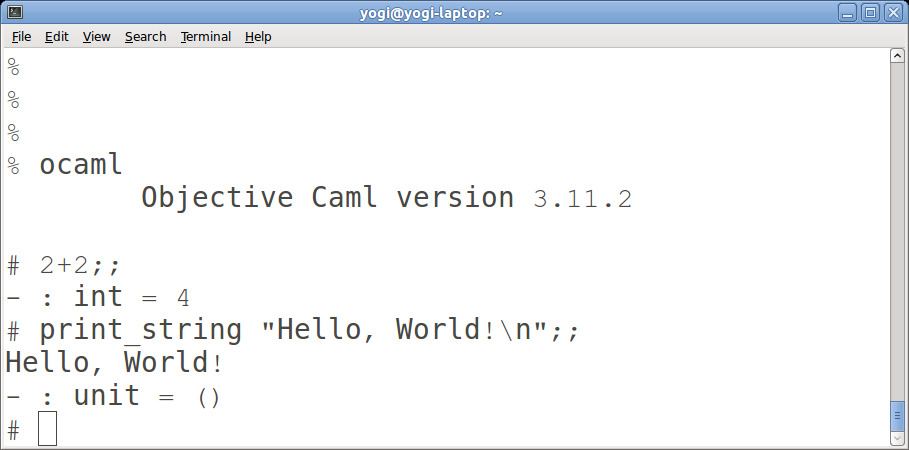
\includegraphics[width=0.8\textwidth]{Screenshot-hello-caml.jpg}
\end{center}
\כיתוב|שימוש אינטראקטיבי בתכנת ocaml|
\תגית|איור:ocaml|
\end{איור}

כפי שאפשר לראות באיור, האינטראקציה שלי עם תכנת ocaml התחילה כאשר הקלדתי
את המילה \קד{ocaml} אל ה\זרז של תכנת bash.
בתגובה, התעוררה תכנת ocaml והציגה עצמה לפני,
\begin{קוד}
\cpp{Objective Caml version 3.11.2}
\end{קוד}
ואחר ביקשה ממני קלט נוסף, בהצגה לי את ה\זרז \קד{#}.
 כאשר הקלדתי אל \זרז זה את הביטוי \קד{2+2},
 תכנת ocaml חישבה את ערכו של הביטוי.
 בתום החישוב, הציגה ocaml את הטיפוס של הביטוי שהקלדתי, \מש{int},
 ואת ערכו, המספר \קד{4}. ולאחר כל אלו חזרה ocaml והציגה לי שוב את ה\זרז, כדי לציין שהיא ממתינה
 לקלט נוסף ממני.

 כאשר הקלדתי אל ה\זרז את הביטוי
 \begin{קוד}
 \let\ttfamily=\listingsfont
 \verb+print_string "Hello, World!\n";;+
 \end{קוד}
 הגיבה ocaml בחישוב הביטוי, ומכיוון שלחישוב זה היתה תוצאת לוואי, הוצג לפני
 הסדרית
 \begin{קוד}
 \listingsfont
 Hello, World!
 \end{קוד}
 לאחר תום החישוב של הביטוי שהקלדתי, הציגה ocaml את הטיפוס של ביטוי זה, \מש{unit}, ואת ערכו
 \קד{()}.\הערת␣שוליים{¢¢
   אולי אינך מבין את פשר הטיפוס \מש{unit} ואת משמעות הערך \קד{()}. משמעותם
 אינה חשובה בשלב זה, והיא תבואר מאוחר יותר, בבואנו לדון בטיפוסים.}

\bash
sed -n /begin/,/end/p < hello.p > hello-body.p
\END

במקום העבודה האינטראקטיבית עם תכנת \שי{ocaml},
יכולתי להכין קובץ המכיל את הקלט אליה:
\begin{קוד}
\bash[script]
cat << EOF >input.caml
2+2;;
print_string "Hello, World!\n";;
EOF
\END
\end{קוד}
ואחרי שהכנתי את הקובץ \קד{input.caml}, אוכל להפעיל את ocaml באופן שבו היא תקרא
ה\קלט שלה מקובץ זה:
\begin{קוד}
\bash[script,stdout]
ocaml < input.caml
\END
\end{קוד}
ה\פלט כולו, כולל ה\זרזים, יוצג על פני המסך. אם לעומת זאת, אפעיל את ocaml
תוך שאני מעביר לה כפרמטר את הקובץ \קד{input.caml}, תכנת ocaml תמנע מלהציג
את הזרז ואת שאר פרטי המידע אותם היא מציגה בעבודה אינטראקטיבית רגילה, אך
תוצאת הלוואי של החישוב תוצג כרגיל:
\begin{קוד}
\bash[script,stdout]
ocaml input.caml
\END
\end{קוד}
אנו רואים כי בשפות תכנות בהן נהוג חישוב אינטראקטיבי, תחילת החישוב היא בפקודה
הראשונה אותה מקליד המשתמש אל ה\זרז. בחישוב אינטראקטיבי יש עדיין צורך להתוות את גבולות התכנית,
כלומר, לקבוע מה כלול בתכנית ומה מחוצה לה. הקביעה נעשית על ידי סביבת העבודה (התכנית ocaml
בדוגמא שלנו), והיא יכולה להיות אוטרקית, מטאפיסית, או הוליסטית.

§ מסגור בלוקים

ציינו למעלה כי ה\פקודות בשפת תכנות מאורגנות בבלוקים, וכי הבלוקים יכולים להיות
מקוננים. מבנה זה הינו כמעט אוניברסלי, אם כי בכל זאת, ישנן שפות מועטות, כמו
פרולוג שבהן ה\פקודות אינן מאורגנות בבלוקים, ואין משמעות ל\קינון.

\קינון של בלוקים יכול לקרות בפקודת תנאי לדוגמא, כאשר התנאי חולש על ביצועו של
הבלוק כולו, וכמובן יתכן כי הבלוק יכיל בלוקים נוספים.

הבדל ויזואלי דקדוקי ברור בין שפות תכנות שונות הוא האופן שבו ממוסגר הבלוק, כלומר
האופן בו מצויינת תחילת הבלוק וסופו. אנו נכנה בשם \פתיח את התו או סדרת תוים
המציינת פתיחתה של ישות ממוסגרת, ואילו השם \בריח ייוחד לתו או לסדרת התוים
המציינת סופה של ישות כזו.

מתכנני שפות התכנות מתחבטים בבחירה המתאימה של ה\פתיח וה\בריח של בלוק פקודות אשר
תקל על המתכנת לזהות בקלות את מבנה התכנית, גם כאשר מבנה ה\קינון של הבלוקים אינו
פשוט.

§§ משפחת שפות הַ-{❴❵}
ראינו שבשפת \סי (\עע תכנית שלום:סי) בלוקים ממוסגרים בסוגריים מסולסלים
\קד{❴❵}.
השפעתה של שפת \סי ושל הגישה המינימליסטית שלה למסגור בלוקים, גדולה
כל כך שמשפחה שלמה של שפות תכנות נקראת על שמה. לעיתים נודעת משפחה זו גם בשם
משפחת שפות הַ-{❴❵}, והיא כוללת בין השאר את שפת \גאוה, שפת \שי{C++}, שפת
\שי{C#}, שפת AWK ועוד.

שפת Go המודרנית הביאה את שיטת הַ-{❴❵} לקיצוניות, בכך שהיא אינה מתירה ל\פקודות
כגון \מש{if} וְ-\מש{while} לחלוש על \פקודה בודדת שאינה ממוסגרת
ב-{❴❵}.

יש הטוענים כנגד קריאותה של שיטת הַ-{❴❵}, משום שהמתכנת נדרש לפרש סימנים מיוחדים
שאינם חלק מהאלפבית הרגיל. התפוצה הרחבה של ממשפחת שפות הַ-{❴❵} יכולה אולי
להוות חיווי לכך שהקושי בלימוד המשמעות של הסימנים המיוחדים הללו אינו גדול כל
כך.

§§ המינימליזם של אוקאם

דרך מינימליסטית אף יותר מזו של משפחת שפות הַ-{❴❵}
הותוותה על ידי שפת התכנות אוקאם\הערת␣שוליים{
  השפה קרוייה על שמו של ויליאם איש אוקאם, שלו מיוחס העיקרון הפילוסופי-לוגי של
התמציתיות, הידוע בשם "תערו של אוקאם".}.
בשפת אוקאם אין \פתיח או \בריח לבלוק של פקודות.
מכיוון שבמילא נוהגים מתכנתים \מונח[הזחה]{להזיח}
פנימה \פקודות הרשומות בבלוק מקונן,
שפת אוקאם קובעת את ה\קינון של בלוקים על פי מידת ה\מונח{הזחה} של הפקודות.

\עע תכנית שלום:אוקאם מדגימה זאת.

\begin{תכנית}
\setLTR
\begin{lstlisting}[language=Ada,style=Numbered,keywords={PROC,SEQ,FOR}]
--Hello world in the Occam programming language
#INCLUDE "hostio.inc"
#USE "hostio.lib"
PROC hello.world (CHAN OF SP fs, ts)
  SEQ
    so.write.string.nl(fs, ts, "Hello, World!")
    SEQ i=1 FOR 10
      SEQ
        so.write.int(fs, ts, i, 0)
        so.write.nl(fs, ts)
\end{lstlisting}
\bash
sed -n /begin/,/end/p < hello.p > hello-body.p
\END

    \כיתוב|"שָׁלוֹם, עוֹלָם!" בשפת אוקאם|
    \תגית|תכנית:שלום:אוקאם|
    \end{תכנית}

    כך למשל ה\פקודות בשורות 8-9 מקוננות ב\פקודה לביצוע סדרתי (\קד{SEQ}) שבשורה
    מס'~7, וזו מצידה מקוננת בלולאה הסדרתית שבשורה מס'~6.

    גישה זו של שפת אוקאם אומצה על ידי שפה פופולרית הרבה יותר, שפת פיית'ון.

    §§ שיטת הַ-\שי{\קד{begin}…\קד{end}}

    הצצה חוזרת ב\עע תכנית שלום:פסקל מראה ששפת פסקל שונה בעליל, בכך שה\פתיח של בלוק
    של \פקודות מסומנת במילה השמורה \מש{begin} ואילו ה\בריח של הבלוק מסומן במילה
    השמורה \מש{end}.
    יש הטוענים כי השימוש במילים מלאות מגדיל את הקריאות של התכנית.

    כנגד טענה זאת, אפשר לומר כי ממילא נדרש הקורא להבין את משמעותן המיוחדת של
    המילים begin וְ-end כאשר נעשה בהן שימוש בשפת התכנות, ומשמעות זו אינה זהה
    למשמעות בשפה הטבעית של מילים אלו.

    בימי קדם, כאשר אוסף התוים השונים הניתן ליצוג על ידי המחשב היה קטן, ואף אוסף
    התוים המוכר במערכת אחת, לא היה בהכרח זהה לזה המוכר במערכת אחרת, היה יתרון
    במסגור בלוקים בשיטת הַ-\שי{\מש{begin}…\מש{end}} שלא דרשה הסתמכות על
    קיומם של סימנים מיוחדים. כך למשל, באוסף התוים הרגיל של חברת \שי{CDC},
    הסימנים \קד{❴} וְ-\קד{❵} לא היו קיימים.

    §§ אזכור הפתיח בסוגר הבלוק.
    ככל שעומק ה\קינון של הבלוקים וככל שמספר ה\פקודות בכל בלוק גדל, הקושי בהבנת מבנה
    התכנית גדל. עיקר הקושי מתעורר כאשר המתכנת מביט ב\בריח, והוא מתקשה בזיהוי
    הנקודה בתכנית שבה נפתח הבלוק.

    יש הנוהגים להוסיף הערה בצמוד ל\בריח בכדי להזכיר את תחילת הבלוק. נוהג
    זה נפוץ יותר במשפחת שפות הַ-\שי{\מש{begin}…\מש{end}}.

    מספר שפות תכנות מרחיבות נוהג זה, בכך שהן מאפשרות, ולעיתים אף מחייבות, הצמדה
    של תזכורת ל\בריח המשייכת אותו ל\ישות תכנותית מסויימת.
    כך למשל ב\עע תכנית שלום:עָדָה הכתובה בשפת עָדָה, כתבנו
    (שורה מס'~6)
    \begin{קוד}
    \ada{end Hello_World;}
    \end{קוד}
    בכדי לציין את סוף הפרוצדורה אשר שמה \קד{Hello\_World}.

    \עע תכנית שלום:אוברון, מציגה דוגמא נוספת, והפעם בשפת אוברון.

    \begin{תכנית}
    \begin{OBERONn}
      MODULE HelloWorld;
      (* Hello, World! in Oberon for the Oberon System *)

      IMPORT Oberon, Texts;

      VAR
      W: Texts.Writer;

      PROCEDURE Do*;
      BEGIN
      Texts.WriteString(W,"Hello, World!");
      Texts.WriteLn(W);
      Texts.Append(Oberon.Log, W.buf)
      END Do;

      BEGIN
      Texts.OpenWriter(W)
      END HelloWorld.
    \end{OBERONn}
    \setRTL
    \כיתוב|"שָׁלוֹם, עוֹלָם!" בשפת אוברון|
    \תגית|תכנית:שלום:אוברון|
    \end{תכנית}

    לא קשה מדי להבין תכנית זו, והפענוח יהיה קל אף יותר אם נזכור ששפה זו תוכננה על
    ידי אותו אדם שתכנן את שפת פסקל.

    בתכנית יש שני בלוקים. שורה מס'~14 מסיימת את בלוק ה\פקודות אשר התחיל בשורה
    מס'~10, ובעצם את הפרוצדורה \קד{Do} שהתחילה בשורה מס'~9.
    זו הסיבה שבשורה מס'~10 נכתב
    \begin{קוד}
    \oberon{End Do}.
    \end{קוד}

    שורה מס'~18 מסיימת את בלוק ה\פקודות אשר התחיל בשורה מס'~16, ויחד עם זאת את
    המודול \קד{HelloWorld} אשר התחיל בשורה מס'~1. זו הסיבה שבשורה מס'~18 נכתב
    \begin{קוד}
    \oberon{END HelloWorld}.
    \end{קוד}

    נשים לב שהפרוצדורה \קד{Do} מצוייה בתוך המודול \קד{HelloWorld}. ה\קינון המודגם
    כאן הוא אם כן לא של בלוק \פקודות בתוך בלוק \פקודות אחר, אם כי, כמובן גם \קינון
כזה יתכן בשפת אוברון.

יש ואריאנטים רבים לשיטת הַ-\שי{\מש{begin}…\מש{end}}.
יש שפות שבהן ה\פתיח הוא המילה השמורה \מש{do} וה\בריח הוא
ה\מונח[מילה שמורה]{מילה השמורה} \מש{done} או
\מונח[מילה שמורה] המילה השמורה \מש{end}, וישנן אף שפות שבהן
אין \פתיח לבלוקים.

§§ שיטת הַ-\שי{\קד{if}…\קד{fi}}
שכלול של שיטת אזכור הפתיח מופיע בשפת אלגול 68. בשפה זו, לבלוק המקונן בפקודת
\מש{if} יש בריח המיוחד רק לו: המילה השמורה \מש{fi}. לבלוק \פקודות המקונן בפקודת
\מש{case} יש בריח יעודי גם כן: המילה השמורה \מש{escac}, ובבלוק המקונן בפקודת
\מש{for...do} המילה השמורה \מש{od} משמשת כ\בריח יעודי. (בעבור לולאות
\מש{repeat}, ה\בריח, באורח טבעי הוא המילה השמורה
\מש{until}, בדומה ללולאת \E|\מש{do}…\מש{while}| בשפת \סי.)

היתרון הוא ברור, אף אם ה\פתיח אינו גלוי, קל לזהות מה\בריח בלבד
את תכנו של בלוק. יהיה אולי אף מי שיאמר שהזוג \שי{\מש{if}…\מש{fi}} הוא תמציתי יותר
מהַ-\שי{\מש{begin}…\מש{end}} ושומר על הקריאות.

כפי ששמה מעיד עליה, שפת אלגול 68, פותחה בשנת 1968.\הערת␣שוליים{
  השם \שי{ALGOL 68} הוא קיצור ל-\שי{ALGOrithmic Language 1968}}
זו הסיבה שהשימוש בשפה זו בעת הזאת נדיר ביותר. אבל, השפעותיה של השפה ושל שיטה
זו ניכרות עד היום. אנו מוצאים מסגור בלוקים מסוג זה, בשפות מעטפת מודרניות (כגון
\שי{bash}), כמו גם במייפל, אחת המערכות הפופולריות ביותר כיום לחישוב מדעי.

§ מפרידים לעומת מסיימים
לאחר שעיינו בשיטות הנפוצות לכתיבת ה\פתיח וה\בריח, מעניין לבדוק כיצד מובדלות
זו מזו ה\פקודות בתוך הבלוק.

\bash
sed -n /begin/,/end/p < hello.p > hello-body.p
\END

§§ דקדוק ספראטיסטי
על פי הגישה הספראטיסטית הנוהגת בשפת פסקל למשל, ה\פקודות בתוך הבלוק מופרדות על
ידי \מפריד, סימן מיוחד. משמעות הפרדת ה\פקודות היא שאם בבלוק יש~\(n$ \פקודות, אזי
יש בו~\(n-1$ \מפרידים. בפרט, אם בבלוק יש \פקודה אחת בלבד,
אז אין בתוך הבלוק אף \מפריד.

כך, ב\עע תכנית שלום:פסקל הכתובה בפסקל, יש רק \פקודה אחת, והתו \קד{;} אינו
מופיע בתוך ה-\שי{\מש{begin}…\מש{end}} העוטף.

גישה זו מכלילה במובן מסויים את הדקדוק של העברת פרמטרים לפונקציות ופרוצדורות. אם
לפונקציה יש ארבעה ארגומנטים, הרי בין הארגומנטים יפרידו שלושה סימני פיסוק.

הקושי בדקדוק הספראטיסטי הוא בכך שבמהלך כתיבת התכנה יש שינויים תדירים ב\פקודות
אשר בבלוק. לא ניתן להעביר \פקודה מבלוק אחר למשנהו מבלי לבדוק כי מספר ה\מפרידים
הן במקור ובמטרה ממשיך להיות קטן באחד ממספר ה\פקודות.

דקדוק ספראטיסטי מקל מתיר גם \פקודה ריקה. בדקדוק זה,
חוקי לכתוב את בלוק ה\פקודות שב\עע תכנית שלום:פסקל הן באופן שבו כתבתי למעלה,

\bash
sed -n /begin/,/end/p < hello.p > hello-body.p
\END

\begin{קוד}
\lstinputlisting
[language=Pascalx,style=display]
{00/hello-body.p}
\end{קוד}
שבו בתוך הבלוק יש בדיוק \פקודה אחת, והן באופן הבא
\bash
sed 's/)/);/' < hello-body.p > hello-body-semi.p
\END
\begin{קוד}
\lstinputlisting
[language=Pascalx,style=display]
{00/hello-body-semi.p}
\end{קוד}
שבו בבלוק הזה יש שתי \פקודות, כאשר השניה מתוכן ריקה.

    אי נוחות גדולה יותר בדקדוק הספרטיסטי היא תוצאה מכך שתו הַנקודה-ופסיק ה\מפריד אינו חלק
    מה\פקודה. כך, מותר אמנם לכתוב,
    \begin{קוד}
    \begin{lstlisting}[language=Pascalx,style=code]
function max(a,b: Integer):Integer;
begin
  if a > b then
     max :=b
  else
     max :=a;
end
    \end{lstlisting}
    \end{קוד}
    אולם, הכתיב הדומה, שבו הוספנו תו נקודה-ופסיק אחרי ה\פקודה \קד{max :=b}
    \begin{קוד}
    \begin{lstlisting}[language=Pascalx,style=code]
function max(a,b: Integer):Integer;
begin
  if a > b then
     max :=b;
  else
     max :=a;
end
    \end{lstlisting}
\end{קוד}
אינו חוקי, משום שבין \מש{then} ובין ה-\מש{else} מותרת רק \פקודה אחת, ואילו במה
שמופיע למעלה יש שתי \פקודות: ראשית, \קד{max :=a} ומיד אחריה, ה\פקודה הריקה.

§§ דקדוק טרמינסטי
בדקדוק טרמינסטי, הנוהג בשפת \סי, ובכמעט כל השפות האחרות במשפחת הַ-{❴❵}, תו
הַנקודה-ופסיק אינו מפריד בין \פקודות, כי אם מסיים אותן. למעשה, תו הַנקודה-ופסיק הוא חלק בלתי נפרד מה\פקודה.

הבלוק הראשי בתכנית "שָׁלוֹם, עוֹלָם!" בשפת \סי (\עע תכנית שלום:סי), היה מורכב
משתי \פקודות על כן:

 \begin{קוד}
\begin{lstlisting}[language=C,style=code]
  printf("Hello, World!\n");
  return 0;
\end{lstlisting}
\end{קוד}
שכל אחת מהן מסתיימת בתו הַנקודה-ופסיק.

הניסיון מוכיח שהדקדוק הטרמיניסטי נוח יותר, במובן זה, שמתכנתים נוטים פחות לשגות
בו. בפרט, פקודת תנאי בשפות כאלו היא סימטרית יותר.

§§ דקדוק ספראטיסטי-טרמיניסטי

ישנו מיזוג של הדקדוק הספראטיסטי (הרגיל, לא זה המקל) והטרמינסטי, שבו אמנם
ה\פקודות מופרדות על ידי תו הַנקודה-ופסיק, אלא שניתן, לפי בחירת המתכנת, להוסיף
תו \קד{;} בסוף סדרת ה\פקודות.

במיזוג זה, ההעתקה וההעברה של \פקודות מבלוק אחד לאחר, היא קלה הרבה יותר. בכל
זאת, המכשלה של איסור הוספת הַנקודה-ופסיק בפקודת המקוננת בפקודת \מש{if} בעינה
עומדת, זאת שכן בין ה-\מש{then} לבין ה-\מש{else} מותר עדיין לשים רק \פקודה אחת
ויחידה.

§§ דקדוק ליברלי

עם התפתחות תורת ההידור, התברר שסימן הַנקודה-ופסיק הוא מיותר במרבית המקרים,
וה\מהדר יכול להסיק בעצמו את מקום סיום ה\פקודה. הדקדוק הליברלי מכליל את הדקדוק
הספראטיסטי-טרמינסטי, בכך שעל פיו, סימן הַנקודה-ופסיק הוא אופציונלי לא רק בתום
הסדרה, אלא בתום כל \פקודה.

דקדוק ליברלי נהוג בשפות חדישות רבות, ובכלל אלו, שפת אייפל, שפת \שי{AWK}, ושפת
\שי{Go}. במקצת המקרים, המהדיר מסתמך על ההנחה כי בכל שורה מצויה \פקודה אחת לכל
היותר, כדי להסיק את מיקום סיום ה\פקודה, אם כי ניתן לראות שהנחה זו אינה חיונית.

שפת Go מגדילה לעשות בכך שסביבת הפיתוח שלה מוחקת באורח אוטומטי מקובץ התכנית
סימני נקודה-ופסיק אשר אותם יכול ה\מהדר להסיק בעצמו.

§ הערות
כל אחת מתכניות "שָׁלוֹם, עוֹלָם!" שראינו, הכילה הערה ובה צויין כי זוהי תכנית
"שָׁלוֹם,עוֹלָם!". בהערה זו ננקב גם שם שפת התכנות בה נכתבה התכנית.

עיון בוחן ב\הערות הרבות שראינו יגלה כי יש הדקדוק של ה\הערות נופל לאחת מבין שתי
תבניות: \הערות שורה ו\הערות בלוק.

§§ הערות שורה
\הערות שורה משתרעות על פני שורה אחת, כאשר בדרך כלל, ההערה מתחילה ב\פתיח וממשיכה
עד סוף השורה, כלומר סימן סוף השורה הוא ה\בריח. יוצאת מכלל זה היא שפת
פורטרן, שבה הערה משתרעת תמיד על פני שורה שלמה.

כפי שראינו בשפת \שי{AWK} (\עע תכנית שלום:AWK), בשפה זו, ה\פתיח הוא סימן
ה\סולמית \קד{#}, וכך גם הדבר בשפות סקריפט רבות ובכללן \שי{bash}.

בשפות ממשפחת הַ-{❴❵}, ה\פתיח של \הערות שורה הוא בדרך כלל זוג \לוכסנים,
\קד{//}. כך הדבר בשפת \שי{Go} (\עע תכנית שלום:Go) ובשפת \גאוה (\עע תכנית
שלום:גאוה). בתחילה שפת \סי לא התירה \הערות שורה, אך גירסאות מודרניות של הגדרת
השפה התירו \הערות שורה, וכמובן ה\פתיח של אלו הוא \קד{//}.

בשפת עָדָה (\עע תכנית שלום:עָדָה), ה\פתיח של \הערות שורה הוא זוג מקפים, \קד{-{}-},
וכך גם הדבר בשפת אוקאם (\עע תכנית שלום:אוקאם) ובשפת אייפל. בשפת אייפל ניתן
גם להשתמש במילה השמורה \מש{note} כ\פתיח, כמודגם ב\עע תכנית שלום:אייפל, תכנית
"שָׁלוֹם, עוֹלָם!" בשפה זו.

\begin{תכנית}
\begin{EIFFELn}
  note "Hello World in the Eiffel programming language"
  class HELLO
  create run
  feature run
  do
  print ("Hello, World!%N")
  end
  end HELLO
\end{EIFFELn}
\כיתוב|"שָׁלוֹם, עוֹלָם!" בשפת אייפל|
\תגית|תכנית:שלום:אייפל|
\end{תכנית}

§§ הערות בלוק
\הערות בלוק הן \הערות התחומות בין \פתיח יחודי ו\בריח יחודי. \הערות כאלו יכולות
להשתרע על פני מספר שורות, או על חלק משורה.

ראינו למשל \הערות בלוק בשפת \סי, שבה ה\פתיח של \הערות הוא זוג התוים \קד{/*}
(כלומר, \לוכסן, ואחריו \כוכבית) ואילו ה\בריח הוא \קד{*/} (\כוכבית ואחריה
\לוכסן). הערות בלוק הופיעו גם בשפת אוברון ובשפת \שי{OCaml}. בשתי שפות אלו,
ה\פתיח היה \קד{(*} (תו פתיחת סוגריים, ואחריו \כוכבית) וה\בריח היה ב-\קד{*)}
(תו סגירת סוגריים, ואחריו \כוכבית).

יש יתרון בקביעת \בריח הערה אשר בו שני תוים או יותר, שכן אם ה\בריח היה מורכב
מתו אחד בלבד, לא היה ניתן להשתמש בתו זה כלל בתוך ההערה. ב\הערות בשפת פסקל בהן
ה\פתיח הוא \קד{❴} (פתיחת סוגריים מסולסלים) וה\בריח הוא \קד{❵} (סגור סוגריים
מסולסלים), לא ניתן כלל להשתמש בתו סגירת ההערה, \קד{❵}, בתוך הערה. זו ככל
הנראה הסיבה ששפת פסקל מתירה גם \הערות בסגנון שראינו באוברון וב-\שי{OCaml},
כלומר \הערות בהן ה\פתיח הוא \קד{(*} וה\בריח הוא ב-\קד{*)}.

\הערות בלוק נוחות מעט יותר מ\הערות שורה לכתיבת \הערות ארוכות הפרושות על פני
מספר שורות, שכן אין צורך לחזור על ה\פתיח בכל שורה ושורה. כך למשל, בהערת הבלוק
בשורות 3--1 ב\עע תכנית שלום:פסקל{}:

\bash
sed '1,/HelloWorld/!d' hello.p > hello-comment.p
\END

\begin{קוד}
\lstinputlisting[language=Pascalx,style=display]{00/hello-comment.p}
\end{קוד}

תווי עזר, כלומר סימונים שאינם שייכים לגוף ההערה הופיעו רק בתחילתה ובסופה.
לעומת זאת, בהערת הפתיחה של \עע תכנית שלום:גאוה, הכתובה בשפת \גאוה, כתבנו את
הערת פתיחת התכנית בסגנון של הערת שורה, היה צורך לחזור על זוג הלוכסנים המהווה
את ה\פתיח בכל שורה ושורה:
\begin{קוד}
\bash
grep // Hello.java > Hello-comment.java
\END
\lstinputlisting[language=Java,style=display]{00/Hello-comment.java}
\end{קוד}
בכל זאת, מסתבר, שמתכנתים נוהגים לעטר את \הערות הבלוק תוך שימוש בסימנים מיוחדים
כדי להבליט את היותן שונות מקוד התכנית. כך עשיתי אף אני בהערה הפותחת את \עע
תכנית שלום:סי{}:

\begin{קוד}
\bash
sed '1,/\*\//!d' hello.c > hello-comment.c
\END
\lstinputlisting[language=C++,style=display]{00/hello-comment.c}
\end{קוד}

שפות רבות תומכות בשני סוגי ה\הערות, כך בשפת \גאוה, שפת \שי{C++}, ושפת
\שי{Go}, ניתן לכתוב הן \הערות שורה באמצעות זוג \לוכסנים, והן \הערות בלוק
הלכודות בין \קד{/*} לבין \קד{*/}.

§§ הערות מקוננות
בדרך כלל, ה\פתיח של הערת בלוק שונה מה\בריח שלה, דבר המאפשר, לפחות עקרונית,
לכתוב הערה המכילה בתוכה טכסט שאף הוא מהווה הערה חוקית. היתרון ב\קינון \הערות
כזה הוא האפשרות ליטול קטע קוד הכולל בתוכו \הערות, ולהפוך את כולו להערה,
באמצעות עטיפתו בזוג של \פתיח ו\בריח.

למרות שליכולת לקנן \הערות יש חשיבות בתחזוקה של תכניות, הן בפסקל והן בשפת \סי,
התמיכה ב\קינון אינה מפותחת. בשפת \סי לא ניתן ל\מונח[קינון]{קנן} \הערות כלל,
וה\בריח הראשון בהערה סוגר את ההערה כולה, ללא תלות במספר ה\פתיחים המצויים בתוך
ההערה לפניו.

ההגדרה הרשמית של שפת פסקל אף היא אוסרת על \הערות מקוננות. בכל זאת, מימושים של
ה\מהדר נוטים להתיר זאת. לעיתים ההיתר הניתן על ידי ה\מהדר הוא ל\קינון \הערות
מסוג \שי{\mbox{\קד{(*}…\קד{*)}}} בתוך \הערות מסוג \שי{\mbox{\קד{❴}…\קד{❵}}}
ולהיפך.

שפת אלגול 68, שבה נהוגות \הערות בלוק, היא יחודית בכך שה\פתיח של הערה זהה
ל\בריח שלה. אנו נשתמש במונח \גדר לציון סדרה של תו אחד או יותר, שמשמשת הן
כ\פתיח והן כ\בריח. ובאופן כללי יותר, \גדר מפרידה בין שני קטעי טכסט הגובלים זה
בזה.

באלגול 68 יש חמש \מונח[גדר]{גדרות} הערה שונים. אם הערה נפתחה על ידי \גדר
מסויימת הרי סגירתה חייבת להיות על ידי \גדר הזהה לה, ועל כן ההערה תוכל להכיל כל
אחד מארבעת ה\גדרות האחרות.

ישנן שפות המכלילות שיטה זו, ומאפשרות לכותב להגדיר ב\פתיח של הערה את ה\בריח
שלה, אך מנגנון זה נדיר. ההנחה המובלעת בתכנון שפות תכנות היא כי על אף שהצורך
בקינון הערות קיים, יש למתכנת אפשרויות אחרות להתמודד עם המקרים הקשים במיוחד,
שהם נדירים יחסית.

\קינון של \הערות שורה הוא קל: הקדמת שורת הערה בסימן פתיחת ההערה שומרת על כך
שהשורה היא שורת הערה. כך ניתן בקלות להפוך קוד ארוך להערה, אף אם הוא כולל
\הערות. הנה לדוגמא שימוש בתכנית sed כדי להפוך להערה את כל \עע תכנית שלום:גאוה
שכתבתי
\begin{קוד}
\bash[script,stdout]
cat Hello.java | sed s+/+//+
\END
\end{קוד}
גם ההפיכה חזרה היא קלה, והיא נעשית באמצעות מחיקה של \פתיח הערת השורה הראשון
בכל בשורה, וזאת בכל השורות שנהפכו להערה.

\begin{קוד}
\bash[script,stdout]
cat Hello.java | sed s+/+//+
\END
\end{קוד}

§§ סמנטיקה של הערות
בדרך כלל, מעבד השפה מתעלם לחלוטין מ\הערות, והן מושלכות בשלב מוקדם של העיבוד.
שפת \סי, ה\הערות מוסרות על ידי המעבד המקדים, כפי שאפשר להיווכח על ידי חיפוש
לוכסן בפלט של המעבד המקדים:

החל{קוד}
bash[script,stdout]
pp -P hello.c | grep / | wc
END
סוף{קוד}

שפות מודרניות יותר, ישנה מגמה של מתן משמעות ל\הערות. בשפות כמו \גאוה, אייפל
פיית'ון, ה\הערות, כולן או מקצתן, יכולות להיות מעובדות בכדי ליצור תיעוד של
תכנית. כך, בשפת \גאוה, \הערות המתחילות ב\פתיח \שי{\קד{/**}} (\לוכסן, ואחריו
תי כוכביות) מעובדות לכדי יצירת תיעוד לתכנית.

דקדוק של שפת אייפל אף מגדיר מקומות מסויימים בתכנית בהם יכולות להופיע \הערות,
קובע לאילו \ישויות שייכות \הערות המופיעות במקומות אלו.

מילולוני סדרית
ין זה מפתיע שבכל אחת מתכניות "שָׁלוֹם, עוֹלָם!" שראינו, הופיעה \מילולון של ה\סדרית
שָׁלוֹם, עוֹלָם!". אך, מפתיע אולי לגלות, כי חרף השוני בין השפות, \מילולונים אילו
ומים מאוד.

\begin{טבלא}[!htb]
קטן
\begin{center}
\let\ttfamily=\listingsfont
\begin{tabular}{|r|l|c|}
\hline
\RL{שפה} & \hfill \מילולון \hfill & סימון סוף שורה ⏎
\hline
\RL{\CPL}, \E|Go|, \E|OCaml| & \LR{\verb+"Hello, World!\n"+} & \verb+\n+⏎
\RL{קובול,פסקל} & \verb+'Hello, World!'+ & ⏎
\LR{AWK},אוברון, עָדָה, \גאוה,אוקאם & \LR{\verb+"Hello, World!"+} & ⏎
\E|אייפל| & \LR{\verb+"Hello, World!%N"+} & \verb+%N+⏎
\hline ⏎
\end{tabular}
\end{center}
\כיתוב|מילולוני הסדרית \קד{Hello, World!} בתכניות "שָׁלוֹם, עוֹלָם!" בשפות השונות|
\תגית|טבלא:מילולונים|
\end{טבלא}

\עע טבלא מילולונים מסכמת את האופן שבו נכתבו המילולונים השונים בתכניות "שָׁלוֹם,
עוֹלָם!" שהוצגו בפרק זה. ובאמת, על פי הטבלא, כמעט שאין הבדלים בין השפות. בכל
השפות שראינו, הערות מצויינות על ידי \גדרות (ולא על ידי \פתיח השונה מה\בריח).

ישנן שפות, כמו פסקל וקובול, בהן ה\גדר של מילולונים הוא הגרש בודד (\קד{'}), אך
במרבית השפות שראינו, ה\גדר הוא תו צמד גרשיים (\קד{"}). ישנן שפות כמו אייפל בהן
סימן סוף השורה כלול בתוך המילולון, וישנן שפות כמו \גאוה בהן הצגת שורה חדשה
בתום הצגת הסדרית נעשתה על ידי קריאה ל\שגרה הנכונה.

מראית ההבדלים תצטמצם אולי עוד יותר בידענו כי ניתן בשפות מסויימות
לבחור בין הכתיב
\begin{קוד}
\let\ttfamily=\listingsfont
\verb+'Hello, World!'+
\end{קוד}
כלומר, שימוש בתו (\קד{'}) כגדר, ובין הכתיב
\begin{קוד}
\let\ttfamily=\listingsfont
\verb+"Hello, World!"+
\end{קוד}
כלומר שימוש בתו (\קד{"}) כגדר.
כך הדבר בשפת קובול, ואכן, אם נבדוק היטב את \עע תכנית שלום:קובול,
נגלה שם מילולון סדרית בשורה מס'~18 התחום בין שני גרשיים כפולים.
\begin{קוד}
\cobol{DISPLAY " " LINE 1 POSITION 1 ERASE EOS.}
\end{קוד}
כך גם קורה במימוש של שפת פסקל בסביבת העבודה שלי.
אם אחליף את התו \cpp{'} בתו \cpp{"} בקובץ \קד{hello.p},
אקבל תכנית תקינה, אשר פעולתה זהה לתכנית המקורית.

\bash[script,stdout]
sed s/\'/\"/g < hello.p > hello\".p; pc hello\".p; ./a.out
\END
שים לב כי שלוש הפקודות לעיל יוצרות קובץ חדש,
{\let\ttfamily=\listingsfont\RL{\verb+hello".p+}},
מתוך הקובץ
{\let\ttfamily=\listingsfont\RL{\verb+hello.p+}}%
~(א),
מהדרות אותו~(ב), ומריצות את התוצאה~(ג) כדי לבדוק שאכן, החלפת הגרש הבודד בגרשיים
לא שינתה דבר ממשמעות התכנית.
\bash[script,stdout]
sed s/\'/\"/g < hello.p > hello\".p; pc hello\".p; ./a.out
\END

כדאי גם להעיר שאף העובדה שאחדות מהתכניות משתמשות בפונקציה אשר מוסיפה
את סימן סוף השורה, אף היא אינה עקרונית במיוחד. כך, בשפת \גאוה,
היה ניתן לכתוב
\begin{קוד}
  \begin{JAVA}
System.out.print("Hello, World!\n");
  \end{JAVA}
\end{קוד}
מבלי לשנות דבר ממשמעותה של התכנית.
\bash[script,stdout]
sed s/\'/\"/g < hello.p > hello\".p; pc hello\".p; ./a.out
\END

§ תכנון דקדוק עבור מילולוני סדרית
התמונה העולה מסקירת \עע טבלא מילולונים מטעה במקצת, שכן טבלא זו כמעט שאינה מגלה
את השאלות הלא פשוטות המתעוררות בתכנון הדקדוק בעבור מילולוני סדרית.
\bash[script,stdout]
sed s/\'/\"/g < hello.p > hello\".p; pc hello\".p; ./a.out
\END

ראשונה לשאלות אלו עוסקת באפשרות לכלול בתוך המילולון את סדרית ה\גדר עצמה.
בעיה כזו מתעוררת כאשר למשל תכנית \סי ליישום חשבונאי מנסה להדפיס דין וחשבון על
רווחים והפסדים, אשר כותרתו 'דו"ח רו"ה' מכילה בעצמה את סימן הגרשיים, או במחוללי
ישומים, שבו הפלט של תכנית הוא תכנית.
\bash[script,stdout]
sed s/\'/\"/g < hello.p > hello\".p; pc hello\".p; ./a.out
\END

שים לב לכך שלמרות שבדוגמאות שב\עע טבלא מילולונים, ה\פתיח וה\בריח היו זהים,
ישנן שפות בהן אין הדבר כך. כך למשל בשפת \שי{\textsc{PostScript}}, הפתיח הוא
סימן פתיחת הסוגריים~\קד{(} וה\בריח הוא סימן סגירת הסוגריים~\קד{)}, כמודגם
בתכנית \עע תכנית שלום:PostScript.
\bash[script,stdout]
sed s/\'/\"/g < hello.p > hello\".p; pc hello\".p; ./a.out
\END

\begin{תכנית}
\setLTR
\lstset{language=Postscript,style=numbered}
\begin{lstlisting}
% Hello, World in Postscript
%!PS
/Palatino-Roman findfont
100 scalefont
setfont
100 100 moveto
(Hello, World!) show
showpage
\end{lstlisting}
\setRTL
\כיתוב|"שָׁלוֹם, עוֹלָם!" בשפת \textsc{PostScript}|
\תגית|תכנית:שלום:PostScript|
\end{תכנית}

ניתן לנסח שאלה זו באורח מעט כללי יותר בהקשר של מציאת דרך לציין תת-סדרה של תוים
מתוך סדרה ארוכה יותר. בהקשר זה בעיית \מונח{גידור הגדר} היא הבעיה של הכללת הגדר
עצמה בתוך תת-הסדרית המסומנת על יד ה\גדר. ברור שששאלת \מונח{גידור הגדר} עשויה
להתעורר אף אם תת-הסדרה תחומה על ידי \פתיח ו\בריח שאינם זהים. כך למשל, בשפת
\E|\textsc{PostScript}|, מתעוררת השאלה במקרה שבו יש צורך להדפיס סדרית המכילה
את סימן סגירת הסוגריים. מאליו ברור שהשאלה הכללית מתעוררת גם במקרה שבו ה\גדר
מכילה יותר מאשר תו אחד.

ניסוח כללי זה מתאים גם למילולונים (הסדרה היא התכנית כולה, ותת-הסדרה היא
המילולון), וגם לדיון שלנו בהערות בלוק מקוננות (הסדרה היא התכנית כולה, תת-הסדרה
היא ההערה, וה\גדר היא ה\בריח של ההערה).

§§ הצהרת האורך
דרך פשוטה להתמודד עם בעית \מונח{גידור הגדר} היא לכתוב ב\פתיח של המילולון את
אורכה של תת-הסדרה. באופן זה, אין כל מגבלה על תכנה של תת הסדרה. ב\עע
תכנית שלום:פורטרן, הכתובה בגירסה ישנה של שפת פורטרן (\שי{FORTRAN 66}) נעשה
שימוש בדרך זו בדיוק.

\begin{תכנית}
\setLTR
\lstset{language=[77]Fortran,style=Numbered,morecomment=[f]C}
\begin{lstlisting}
 PROGRAM HELLO
 A HELLO, WORLD! PROGRAM IN FORTRAN IV
 WRITE (6,100)
 FORMAT(14H HELLO, WORLD!)
 STOP
 END
\end{lstlisting}
\setRTL
\כיתוב|"שָׁלוֹם, עוֹלָם!" בשפת פורטרן 66|
\תגית|תכנית:שלום:פורטרן|
\end{תכנית}

בשורה המסומנת במספר 100, יש מה שקוראים \מונח{קבוע הולרית'} המסומן באות \שי{H}. סדרת
שלושת התוים \שי{14H} המופיעה בשורה זו מציינת שאחריה יופיע מילולון בן 14 תוים,
ואכן ספירה מדוקדקת וזהירה תגלה שב\סדרית{}
{\let\ttfamily=\listingsfont\LR{\verb*+HELLO, WORLD!+}}
יש 14 תוים בדיוק (ובלבד שלא נשכח לספור את סימן הרווח הפותח את הסדרית הזו).
מאליו ברור הדבר שעל אף היתרונות של השיטה ההצהרתית הזו לסימון מילולונים, השימוש
בה על ידי בני תמותה אינו קל.

\bash[script,stdout]
sed s/\'/\"/g < hello.p > hello\".p; pc hello\".p; ./a.out
\END

השיטה ההצהרתית נכחדה משימוש. כבר בפורטרן 77, בוטל השימוש
ב\מונח[קבוע הולרית']{קבועי הולרית'}.
בכל זאת, יש לשיטה קיום כדרך יעילה לתיחום של סדריות המיוצרות ונקראות על ידי מחשב.
\bash[script,stdout]
sed s/\'/\"/g < hello.p > hello\".p; pc hello\".p; ./a.out
\END

§§ שיטת המילוט
השיטה המקובלת כיום לפתרון בעית \מונח{גידור הגדר} ברוב שפות התכנות היא זו של
\מילוט, ובה תו מיוחד, \מונח{תו ממלט} אשר נותן משמעות מיוחדת לתו המופיע אחריו.
בפרט, מופע של תו המילוט מונע מהגרשיים (או כל תו אחר המשמש כ\גדר) לסגור את
תת-הסדרית. מקובל להשתמש ב\מונח{לוכסן הפוך} כתו המילוט, אך מוכרים גם תוי מילוט
אחרים.
\bash[script,stdout]
sed s/\'/\"/g < hello.p > hello\".p; pc hello\".p; ./a.out
\END

שיטת ה\מילוט מתאימה גם למקרה שבו ה\גדר היא בת מספר התוים: \מילוט תו כלשהו, בדרך
כלל התו הראשון, של סדרת התווים המהוה את ה\גדר מונע מסדרה זו מלהיות \גדר.
\bash[script,stdout]
sed s/\'/\"/g < hello.p > hello\".p; pc hello\".p; ./a.out
\END

שיטת המילוט דורשת כמובן דרך למלט את \מונח[תו ממלט]{התו הממלט} עצמו. בדרך כלל
מופע בודד של \מונח[תו ממלט]{התו הממלט} בתוך המילולון מצויין באמצעות סדרה של
שני תוים כאלו.
\bash[script,stdout]
sed s/\'/\"/g < hello.p > hello\".p; pc hello\".p; ./a.out
\END

כדי להבין ענין זה על בוריו, נחזור ונסתכל על \עע תכנית שלום:OCaml, תכנית
"שָׁלוֹם, עוֹלָם!" בשפת \שי{OCaml}. האתגר הוא בכתיבת תכנית בשפת \סי, שפה המשתמשת
בשיטת המילוט, אשר הפלט שלה יהיה \עע תכנית שלום:OCaml. בכדי לקצר, נסתפק בהדפסת
ה\פקודה הביצועית הבודדת ב\עע תכנית שלום:OCaml{}:


\bash
grep print hello.caml > hello-core.caml
\END

\begin{קוד}
\setLTR
\lstset{language=[Objective]Caml,style=display}
\lstinputlisting{00/hello-core.caml}
\end{קוד}

בכדי להדפיס פקודה זו מתוך תכנית \סי, יהיה צורך למלט את הגרשיים הכפולים וכן
יהיה צורך למלט את \מונח[לוכסן הפוך]{הלוכסן ההפוך} המופיע לפני האות \קד{n}.
כמודגם ב\עע תכנית מילוט:סי, כדי להדפיס את הפקודה לעיל, נדרשים בסה"כ-חמישה
מופעים של תו המילוט.
\bash
grep print hello.caml > hello-core.caml
\END

\bash
rm -f make-hello-caml.c
cat << EOF > make-hello-caml.c
#include <stdio.h>
int main(int argc, char *argv[], char **envp) {
  printf("print_string \"Hello, World!\\\\n\";;\n");
  return 0;
}
EOF
cc make-hello-caml.c
rm -f hello-made-by-c.ml
./a.out >hello-made-by-c.ml
ocaml hello-made-by-c.ml
\END

{
\setLTR
\lstinputlisting[language=C++,style=Numbered]{00/make-hello-caml.c}
}

\bash
cc make-hello-caml.c; ./a.out
\END
\begin{תכנית}
\bashStdout
\כיתוב|מילוט בשפת \סי|
\תגית|תכנית:מילוט:סי|
\end{תכנית}

קושי נוסף ששיטת המילוט טומנת בחובה הוא ברמת סיבוך נוספת בהפעלתם של ביטויים
רגולריים. חיפוש ב\עע תכנית מילוט:סי אחר סימון סוף השורה הרגיל בשפת \סי (הרצף
{\let\ttfamily=\listingsfont\RL{\verb+\n+}}) עלול לאתר שניים כאלו, אך למעשה,
בתכנית זו יש רק מופע אחד של התבנית הזו. מה שנדרש כדי לאתר מופע של סימון זה,
הוא ביטוי רגולרי המחפש את האות \קד{n} המופיעה אחרי מספר אי זוגי של מופעים של
תו הלוכסן ההפוך.

לעומת חסרונות אלו, יתרון חשוב של שיטת המילוט, הוא בכך שהיא מאפשרת לכלול
בתוך המילולון תוים מיוחדים אחרים, אשר אין להם יצוג גרפי, או שהיצוג הגרפי
שלהם יכול להיות מטעה. כך ראינו כי את תו השורה החדשה ניתן לסמן באמצעות
{\let\ttfamily=\listingsfont\RL{\verb+\n+}},
וסימונים אחרים כאלו
ישנם למכביר. בשפת \סי ניתן גם להכניס אל תוך \מילולון כל תו מבין 256 תוי
ה-ASCII באמצעות \מונח{תו ממלט} המקדים את מספרו הסידורי של התו המבוקש. שפות
Go ו\גאוה תומכות במספר ההולך וגודל של תוי היוניקוד (כמעט עשתי-עשרה רבבות לעת
כתיבת ספר זה), ניתן לכלול בתוך \מילולון \סדרית כל אחד מהתוים הללו, באמצעות
הקדמת \מונח{תו ממלט} למספרו של התו המבוקש.

שאלה שיכולה להיראות כקנטרנית היא זו של משמעות תו המילוט כאשר הוא מופיע לפני תו
שאין צורך למלטו. כך ניתן להציק ולשאול מה המשמעות של תו הרווח כאשר מופיע לפניו
תו מילוט. מתכנן של שפת תכנות אינו יכול להתעלם משאלה כזו, ועליו להחליט אם לגלות
סובלנות ל"שגיאות" מסוג זה, או להתריע על כך.

לכל אחת משתי האפשרויות יש תג מחיר משלה. התעלמות ממילוט של תו שאין צורך למלטו,
יכולה להביא להתעלמות משגיאות אמיתיות של המתכנת, אשר טעה בבחירת התו הממולט. מצד
שני, התרעה על מילוט כזה, יכולה להטיל מעמסה נוספת על המתכנת, אשר יצטרך להזהר
מלמלט תוים שאותם אין למלט.

§§ הכפלת הגדר

אמרנו למעלה כי שיטת המילוט דורשת דרך למלט את \מונח[תו ממלט]{התו הממלט} עצמו,
וכי מופע בודד של \מונח[תו ממלט]{התו הממלט} בתוך המילולון מצויין באמצעות סדרה של
שני תוים כאלו.

גישה חילופית, ופשוטה מעט יותר משיטת המילוט משתמשת בהכפלת ה\גדר במקום הכפלת
\מונח[תו ממלט]{התו הממלט}. בשיטה, הנוהגת למשל בשפת פסקל ובשפת בייסיק,
התו הממלט הוא למעשה ה\גדר עצמה. על כן, מופע כפול של תו ה\גדר מציין תו זה כפשוטו ורק מופע בודד של תו ה\גדר מציין את
סיום המילולון.

על כן, כדי לכלול~$n$ מופעים של ה\גדר בתוך סדרית, יש לכתוב
אותו~$2n$ פעמים במילולון המגדיר את הסדרית.

לכלל זה יש חריג אחד בלבד:
המילולון המציין את הסדרית הריקה מוגדר על ידי שני מופעים של ה\גדר.

שיטה זו של הכפלת ה\גדר אמנם נקיה יותר, אך בהעדר תו מילוט, יש
להשתמש באמצעי אחר כדי לכלול ב\מילולון תוים נעדרי יצוג גרפי.

הקושי בבנית ביטויים רגולורים אף הוא קיים בשיטת הכפלת הגדר.

§§ ריבוי אפשרויות מסגור
שיטה חילופית נוספת לשיטת המילוט משמשת בשפות בהן ניתן למסגר \מילולון הן בין זוג
של גרשים בודדים והן בין זוג של גרשיים כפולים. בשפות אלו אין מניעה לכלול את
סימן הגרשיים בתוך \מילולון התחום בין גרשים בודדים, או לכלול את סימן הגרש הבודד
בתוך \מילולון התחום בזוג של גרשיים כפולים.

\עע תכנית מילוט:פסקל מדגימה זאת, תוך שימוש בואריאנט של פסקל המותקן בסביבת
החישוב שלי.
\bash
sed -n /output/,/end/p < hello.p > hello-core.p
\END

\bash
rm -f make-hello.p; cat << EOF >make-hello.p
program makeHelloWorld(output);
begin
  WriteLn('program HelloWorld(output);');
  WriteLn('begin');
  WriteLn(" WriteLn('Hello, World!')");
  WriteLn('end.')
end.
EOF
pc make-hello.p; ./a.out >made-hello.p
pc made-hello.p
./a.out
\END

\bash
sed -n /output/,/end/p < hello.p > hello-core.p
\END

\begin{תכנית}
\setLTR
\lstinputlisting[language=Pascalx,style=Numbered]{00/make-hello.p}
\begin{Output}
\bash[stdout]
pc make-hello.p; ./a.out
\END
\end{Output}\setRTL
\כיתוב|שתי דרכים שונות לתיחום מילולונים במימוש גנו של שפת פסקל|
\תגית|תכנית:מילוט:פסקל|
\end{תכנית}

\bash
sed -n /output/,/end/p < hello.p > hello-core.p
\END

אנו רואים כי הפלט של \עע תכנית מילוט:פסקל הוא תכנית "שָׁלוֹם, עוֹלָם!" הכתובה
בפסקל. למעשה הפלט של תכנית זו הוא בדיוק הפקודות הביצועיות של \עע תכנית
שלום:פסקל.

\bash
sed -n /output/,/end/p < hello.p > hello-core.p
\END

בבסיסה, שיטה זו חלשה יותר משיטת המילוט, שכן היא אינה תומכת במילולון המכיל הן
תו של גרש בודד והן תו של גרשיים כפולים. שפת התכנות פרל, ושפות נוספות מכלילות
את השיטה, בכך שהן מאפשרות לקבוע כל תו רצוי כ\גדר ל\מילולון. בשפות אלו, הקושי
היחידי הוא בכתיבת מילולון המכיל את כל התוים כולם.
\bash
sed -n /output/,/end/p < hello.p > hello-core.p
\END

ראינו כבר דוגמא להכללה זו למעלה, כאשר השתמשנו בתכנית sed כדי לסלק
את ה\פתיח של זוג לוכסנים בהערות שורה ב\גאוה:
\begin{קוד}
\ada{sed s+//++}
\end{קוד}
הפקודה \קד{s} של sed מחליפה סדרית אחת באחרת. תחילת הסדרית וסיומה נקבעת על
ידי התו המופיע מיד אחרי הפקודה \קד{s}, לכן בהוראה \שי{\קד{sed s+//++}} התו
\קד{+} משמש כ\גדר, וההוראה כולה מציינת בקשה להחלפה של הסדרית המכילה זוג
לוכסנים בסדרית הריקה. כמובן, היה ניתן לכתוב הוראה זו תוך שימוש בכל תו אחר
כ\גדר. למשל, בכתיב
\begin{קוד}
\bash
sed -n /output/,/end/p < hello.p > hello-core.p
\END

\ada{sed sa//aa}
\end{קוד}
התו \ada{a} משמש כ\גדר, אך משמעות ההוראה לא תשתנה.
\bash
sed -n /output/,/end/p < hello.p > hello-core.p
\END

§§ מילולונים ארוכים ותוים מיוחדים

הסדרית \שי{\קד{"!Hello, World"}} שהצגנו, היתה קצרה ביותר, אך תכניות מחשב נדרשות
לעיתים להציג טכסטים ארוכים. שאלה מעניינת בבחינת הדקדוק של מילולונים היא התמיכה
בסדריות ארוכות היכולים להשתרע על פני מספר שורות.

\bash
sed -n /output/,/end/p < hello.p > hello-core.p
\END

כדי להדגים את השיטות המקובלות לבניית מילולונים ארוכים כאלו, ננסה לכתוב תכנית,
אשר, בדומה ל\עע תכנית מילוט:פסקל, תפיק כפלט את \עע תכנית שלום:פסקל מבלעדי
ההערות, כלומר את ארבעת השורות הבאות:

\bash
sed -n /output/,/end/p < hello.p > hello-core.p
\END

\begin{קוד}
\lstinputlisting[language=Pascalx,style=display]{00/hello-core.p}
\end{קוד}
\bash
sed -n /output/,/end/p < hello.p > hello-core.p
\END

שפת \סי, כמו שפות רבות אחרות, אינה מתירה ל\מילולון{} \סדרית להשתרע על פני
יותר מאשר שורה אחת. הסיבה לכך היא הרצון למנוע שגיאות הידור מוזרות וקשות להבנה
היכולות להיווצר כאשר התכנת שכח להוסיף את ה\גדר הסוגרת את ה\מילולון המתחיל
בשורה מסויימת. לו היה \מילולון יכול להתפרש על פני מספר שורות, שכחה כזו
היתה מביאה לכך שה\מילולון אשר שכח המתכנת לסגור, יתפרש על פני מספר רב של שורות,
ויגמר רק בתחילת ה\מילולון הבא.
\bash
sed -n /output/,/end/p < hello.p > hello-core.p
\END

בכל זאת, בשפת \סי, אם התו האחרון בשורה הוא \מונח{תו ממלט}, המילולון יכול
להמשך על פני השורה הבאה. \עע תכנית מילוט:סוף:שורה עושה שימוש בתכונה זו כדי
להפיק את ארבעת השורות של התכנית "שָׁלוֹם, עוֹלָם!" בשפת פסקל.
\bash
sed -n /output/,/end/p < hello.p > hello-core.p
\END

\renewenvironment{Output}{}{}
\bash
cat <<EOF >make-hello-escape-p.c
#include <stdio.h>
int main(int argc, char *argv[], char **envp) {
  printf(
    "program HelloWorld(output);\n"
    "begin\n"
    " WriteLn('Hello, World!')\n"
    "end.\n");
  return 0;
}
EOF
cc make-hello-escape-p.c;./a.out
\END

\begin{תכנית}
\setLTR
\begin{CPPn}
#include <stdio.h>
int main(int argc, char *argv[], char **envp) {¢¢
  printf(
  "program HelloWorld(output);\
  begin\n\
  WriteLn('Hello, World!')\n\
  end.\n");
  return 0;
}
\end{CPPn}
\begin{Output}
 \bash
 cc make-hello-escape-p.c; ./a.out
\END
\end{Output}\setRTL
\כיתוב|מילוט סוף שורה לשם בנית מילולונים ארוכים בשפת \סי|
\תגית|תכנית:מילוט:סוף:שורה|
\end{תכנית}

בנית \מילולון רב שורות על ידי מילוט סוף השורה כפי שהודגם ב\עע תכנית
מילוט:סוף:שורה, תכשל אם אחרי \מונח[תו ממלט]{תו המילוט} שבסוף השורה יתגנב ולו
תו רווח בלתי נראה אחד. אם כך יקרה, הלוכסן ההפוך, הלא הוא
\מונח[תו ממלט]{תו המילוט} שלנו יתייחס לתו בלתי-נראה זה,
והמשכת ה\מילולון לשורה הבאה תכשל.

אבן נגף זו הוסרה במהדורות חדישות של שפת \סי, אשר קבעו כי שני \מילולונים סמוכים
\מונח[שרשור]{ישורשרו} זה לזה ויהפכו למילולון אחד. שימוש בתכונה זו כדי לבנות
מילולונים ארוכים בשפת \סי מודגם ב\עע תכנית שרשור:מילולונים:סי, אשר מפיקה את
את אותו הפלט של \עע תכנית מילוט:סוף:שורה, אך באורח עמיד יותר בפני שגיאות הקלדה.

\begin{תכנית}
\bash[stdout]
cat <<EOF >make-hello-chain-p.c
#include <stdio.h>
int main(int argc, char *argv[], char **envp) {
  printf("program HelloWorld(output);\n"
  "begin\n"
  " WriteLn('Hello, World!')\n"
  "end.\n");
  return 0;
}
EOF
\END
\setLTR
\lstinputlisting[language=C++,style=Numbered]{00/make-hello-chain-p.c}
\begin{Output}
\bash
cc make-hello-chain-p.c; ./a.out
\END
\end{Output}\setRTL
\כיתוב|יצירת מילולונים ארוכים על ידי שרשור מילולונים סמוכים בשפת \סי|
\תגית|תכנית:שרשור:מילולונים:סי|
\end{תכנית}

בשפת \גאוה אין מנגנון המאחד שני \מילולונים לכדי \מילולון אחד אך אופרטור
החיבור בשפה זו מבצע \מונח{שרשור} של \סדריות.

נשים לב לכך שההבדל בין ה\מונח{שרשור} בשפת \סי לזה של \גאוה, הוא שבשפת \סי,
נוצר \מילולון אחד, טרם ההידור, ואילו ב\גאוה, השרשור נעשה בזמן הריצה. לשון
אחר, בשפת \גאוה אין תמיכה ב\מילולון רב שורות.

\עע תכנית שרשור:מילולונים:גאוה מדגימה שימוש באופרטור השרשור של \סדריות בשפת
\גאוה כדי להפיק את ארבעת השורות של התכנית "שָׁלוֹם, עוֹלָם!" בשפת פסקל.

\bash
cat << EOF > MakePascalHelloWorld.java
class MakePascalHelloWorld {
  static public void main(String args[]) {
    System.out.println(
    "program HelloWorld(output);\n"+
    "begin\n"+
    " WriteLn('Hello, World!')\n"+
    "end.\n"); }}
EOF
\END
\begin{תכנית}
\setLTR
\lstinputlisting[language=Java,style=Numbered]{00/MakePascalHelloWorld.java}
\begin{Output}
\bash
javac MakePascalHelloWorld.java; java MakePascalHelloWorld
\END
\end{Output}\setRTL
\כיתוב|שרשור מילולונים בשפת \גאוה|
\תגית|תכנית:שרשור:מילולונים:גאוה|
\end{תכנית}

שפת Go מציעה תמיכה נוחה במיוחד ב\מילולונים רבי שורות. בשפה זו, אין כל מגבלה על
\מילולונים התחומים על ידי התו \שי{\קד{`}} (גרש בודד הפוך) והם יכולים להכיל
כל תו שהוא, ובפרט גם את סימן סוף השורה.

כתיבת תכנית בשפת Go אשר הפלט שלה הוא ארבעת השורות הללו בפסקל הוא קל במיוחד,
ומודגם ב\עע תכנית מילולון:רב:שורות.
\begin{תכנית}
\setLTR
\begin{GOn}
  package main
  import "fmt"
  func main() {¢¢
    fmt.Printf(
    `program HelloWorld(output);
    begin
    WriteLn('Hello, World!')
    end.`)
  }
\end{GOn}\setRTL
\כיתוב|מילולון סדרית רב-שורות בשפת Go|
\תגית|תכנית:מילולון:רב:שורות|
\end{תכנית}

בתוך \מילולונים ארוכים בשפת Go, אין
\מונח{תו ממלט}, ולוכסן הפוך, אם יופיע שם, מתפרש כפשוטו.

המגבלה העיקרית על תכנם של מילולונים אלו, כתוצאה מבעיית
\מונח{גידור הגדר}, שהם אינם יכולים להכיל את התו \שי{\קד{`}}. בנוסף,
העובדה שרווחים בלתי-נראים בסוף שורה יכולים להתגנב אל תוך מילולונים כאלו
מהווה מטרד מסויים.

\מילולון התחום על ידי \שי{\קד{`}} נועד רק למטרה של כתיבת \סדריות ארוכות. לעומת
זאת, כפי שראינו ב\עע תכנית שלום:Go, \מילולון של Go התחום באמצעות \קד{"} מיועד
לסדריות קצרות, ובו ניתן להשתמש בלוכסן ההפוך כ\מונח{תו ממלט}.

לסיום פרק ראשון זה בכלל, והדיון ב\מילולונים ארוכים בפרט, נשוב אל תחילת הפרק,
שם כתבתי מספר שורות ל-\שי{bash}, אשר הפיקו את תכנית "שָׁלוֹם, עוֹלָם!" בשפת \סי.
נזכר כעת בשורות אלו:
\begin{קוד}
\lstset{basicstyle=\listingsfont\codesize}
\lstinputlisting[language=bash,keywords={},showstringspaces=false=false]
{00/make-hello-c.sh}
\end{קוד}
אנו רואים כי השימוש במה שקראנו "\מונח{מטבע לשון תכנותית}
\begin{קוד}
\cpp{cat << EOF}
\end{קוד}
הוא בעצם מנגנון
לבניית מילולון רב שורות, וכי מנגנון זה הוא גמיש מיוחד באשר ה\פתיח של המילולון
מגדיר את ה\בריח שלו. מפתיע אולי לגלות כי לא היה צורך בכל
מילוט במילולון ארוך זה.
\endinput

\פרק{פרדיגמות}
מי אשר למד שתיים שלוש שפות תכנות "רגילות" כגון C וְ Bash, עלול לחשוב כי לימוד של שפת תכנות חדשה הוא פשוט: יש ללמוד את הדקדוק, ובפרט, כיצד מגדירים משתנים, כיצד כותבים פקודות תנאי, פקודות לולאה, וכיוצ"ב.
בקורס זה נגלה כי הדברים מורכבים מעט יותר: שפות תכנות נחלקות לְפָּרָדִיגְמוֹת, כאשר פָּרָדִיגְמָה היא דרך מחשבה וסגנון תכנות, אשר שפת התכנות מכתיבה למתכנת. המושגים שתוארו מעלה, מופיעים רק בפרדיגמה אחת.
הפרדיגמות העיקריות
ארבעת הפרדיגמות העיקריות הן:
1. הפרדיגמה הַצִּוּוּיִית (Imperative) הנקראת לפעמים גם הפרדיגמה הפרוצדורלית, ואשר השפות C, Bash ופסקל הן דוגמאות שלה.
* בפרדיגמה זו נמצא משתנים, ביטויים, פקודות, כולל פקודות תנאי ופקודות לולאה, פונקציות ופרוצדורות.
* תכנית הכתובה בשפה אימפרטיבית יש בכל רגע מצב (State) המוגדר על ידי תוכן הזיכרון (אוסף המשתנים ה"חיים") ונקודת הריצה הנוכחית.
* תיכנות בפרדיגמה זו נעשה באמצעות ציווי: כתיבת פקודות אשר מצוות על התכנית לשנות את מצבה.
* פקודות בשפה אימפרטיבית יכולות להיות מאוגדות בפרוצדורות.
* אחת הסיבות לכך שהפרדיגמה האימפרטיבית היא הנפוצה ביותר, היא ששפות המכונה הן אימפרטיביות. תרגום תכנית בשפה אימפרטיבית לשפת מכונה יכול להיות על כן יעיל במיוחד.
1. הפרדיגמה הפונקציונלית אשר השפות ML, Haskell, LISP וְ Scheme הן דוגמאות שלה.
* בפרדיגמה זו אין משתנים כלל ואין פקודות.
* את מקום פקודת התנאי מחליף ביטוי מותנה, את הלולאות מחליפה רקורסיה. בפרק התירגול של הקורס שבו נלמד את שפת ML נגלה באורח מפתיע כי ניתן לתכנת ללא שימוש במשתנים כלל.
* כתוצאה מהעדר המשתנים והפקודות, לתכנית אין "מצב" בזמן ריצה, פרט לנקודות החישוב הנוכחית.
* שם הפרדיגמה נובע מכך שפונקציות מהוות את הדרך העיקרית לתיאור החישוב. תכנית בפרדיגמה זו מרבה לחשב ביטויים באמצעות קריאה לפונקציות, להעביר פונקציות כפרמטר לפונקציות אחרות, וכתיבת פונקציות אשר מייצרות ומחזירות פונקציות אחרות.
* נשים לב לכך שבהעדר פקודות, כל שפונקציה יכולה לעשות הוא להחזיר את ערכו של ביטוי, אשר יכול להיות מחושב באמצעות קריאה לפונקציות אחרות, או באמצעות האופרטורים היסודיים.
* שפות פונקציונליות הן לרוב אלגנטיות במובן זה שיש מספר קטן של מושגים אותם יש להבין כדי לתכנת בשפה, וגם במובן זה שהן מאפשרות ביטוי תמציתי של דרך החישוב. באופן טיפוסי תכנית לפתרון בעיה מסוימת בשפה פונקציונלית תהיה קצרה בכמה מונים מתכנית דומה בשפה ציוויית.
1. פרדיגמה מונחית העצמים אשר השפות++C וְ Java הן דוגמאות שלה, אף שאינן שפות תכנות מונחות עצמים טהורות. דוגמאות לשפות שהן מונחות עצמים טהורות יותר הן Eiffel וְ Smallatalk. פרדיגמה זו תילמד בקורס ההמשך 236703 - תכנות מונחה עצמים.
* כדי להדגים את צורת החשיבה השונה בפרדיגמה זו, נסתכל בקטע קוד המקביל לפקודת תנאי בשפת Smalltalk:

\begin{verbatim}
a < b
 ifTrue: [^'a is less than b']
 ifFalse: [^'a is greater than or equal to b']
\end{verbatim}

          \begin{ציינון}
\item בפרדיגמה מונחית העצמים, כל החישוב כולו הוא העברת הודעות לעצמים, אשר
      מגיבים להם בחישוב קצר בהתאם לטיבו של העצם המקבל. כך, a < b שנראה
      כביכול כביטוי, אינו ביטוי כלל וכלל, אלא שליחת ההודעה > עם הפרמטר b
      לעצם a. בתגובה להודעה זו העצם a יחזיר את העצם true או העצם false.
  \end{ציינון}

    \begin{ציינון}
\item לתוצאה המוחזרת תשלח ההודעה
    \end{ציינון}

\begin{verbatim}
ifTrue:…ifFalse:…
\end{verbatim}

      אשר לה שני פרמטרים, שכל אחד מהם הוא בלוק המוכן לחישוב.
\begin{verbatim}
[^'a is less than b']
[^'a is greater than or equal to b']
\end{verbatim}
      כעת, העצם true יחשב את הארגומנט הראשון, ויתעלם מהשני, ואילו העצם false
      יתעלם מהארגומנט הראשון ויחשב את השני.  1. הפרדיגמה הלוגית – אשר שפת
      התכנות Prolog מהווה דוגמא שלה. אף בפרדיגמה זו אין פקודות, משתנים, תנאים,
      ולולאות, אבל בניגוד לפרדיגמה הפונקציונלית, אין בפרדיגמה הזו הגדרת דרך
      חישוב. לעומת זאת, על המתכנת להגדיר תוך שימוש בלוגיקה את מטרת החישוב,
      ו"מָנוֹעַ" פנימי של שפת התכנות יפעל לשם השגת מטרה זו.  החלוקה לפרדיגמות אינה
      תמיד חדה וברורה. בנוסף לפרדיגמות העיקריות, יש פרדיגמות נוספות אשר ההבדלים
      ביניהן הם לעיתים שנויים במחלוקת. עם אלו ניתן למנות את הפרדיגמה המקבילית
      (אשר נלמדת בקורסים אחרים בפקולטה), הפרדיגמה מונחית האספקטים ועוד רבות
      רבות אחרות. בנוסף, ישנן גם שפות המשתייכות למספר פרדיגמות.
      §הפרדיגמה הלוגית
      הפרדיגמה הלוגית מתאפיינת בכך שאין בה לא פקודות הצבה, לא פקודות תנאי ולא פקודות לולאה. בפרדיגמה הזו אין גם פונקציות ולא פרוצדורות, ואין (כמעט) מילים שמורות. בשפות בפרדיגמה הלוגית יש אמנם "משתנים", אך אלו שונים לחלוטין בטיבם מהמשתנים המוכרים לנו בשפות אימפרטיביות.
      במקום כל אלו, תכנית בפרולוג מורכבת משלושה חלקים:
      \ספרר
      \item עובדות יסוד.
      \item כללי היסק.
      \item מטרת החישוב.
      ===
      כל אחד משלושת אלו מנוסח כטענה לוגית. יתירה מכך, עובדות הן למעשה כללי היסק, אשר בסיס ההיסק שלהן ריק. ניתן לכן לקרוא לקבוצת עובדות היסוד וכללי ההיסק אקסיומות, הנכתבות כפרדיקטים לוגיים. המתכנת הכותב בפרולוג, מגדיר אוסף של אקסיומות, ואחר כך, החישוב בפועל מתבצע על ידי הצבת "מטרה", שהיא פרדיקט בלוגיקה.
      בפרולוג יש מנוע פנימי המנסה להוכיח את פרדיקט המטרה מתוך האקסיומות. ההוכחה יכולה להיות של הפרדיקט הכללי, או של מקרים פרטיים של הפרדיקט המתקבלים באמצעות קביעת ערך של משתנים עבורו.
      תוצאת פעולתו של מנוע ההיסק הפנימי של פרולוג עשוייה להיות:
      \begin{ציינון}
\item הוכחת הפרדיקט במלואו (נדיר, אך אפשרי עקרונית)
\item ייצור של מקרים פרטים (עובדות), המקיימות את הפרדיקט. אם מספר העובדות הוא סופי, המנוע יכול לייצר את כולן. אם מספר העובדות הוא אינסופי, המנוע ייצר סדרה אינסופית של עובדות כאלו.
\item הפרכת הפרדיקט, באמצעות הוכחה שהוא אינו יכול להתקיים.
\item לולאה אינסופית,
      טרם תחילת הביצוע בפרולוג, טוען מנוע החישוב מספר רב של פרדיקטים, אשר "מוגדרים מראש" בשפה.
      הנה הדגמה של הרצה בפועל של פרולוג.
  \end{ציינון}

\begin{קוד}
% prolog # try to run prolog
The program 'prolog' can be found in the following packages:
* gprolog
* swi-prolog-nox
Try: sudo apt-get install <selected package>
% sudo apt-get install # install prolog
[sudo] password for yogi:
瞎说
% prolog # invoke the Prolog interpreter from command line
Welcome to SWI-Prolog (Multi-threaded, 瞎说
For help, use ?- help(Topic). or ?- apropos(Word).
?- X==X.
true.

?- X=X.
true.

?- plus(2,2,4).
true.

?- plus(1,1,3).
false.

?- plus(3,X,17).
X=14.
\end{קוד}

בדוגמא לעיל:
\begin{enumerate}
\item הקלט מהמשתמש צבוע באדום, ואילו הפלט אותו מוציא המחשב, צבוע בכחול.
\item במקום שבו ראינו לקצר ולא לפרט את הפלט המלא' החלפנו אותו בסימנים 瞎说 אשר את פענוח משמעותם בשפה הסינית נותיר לקורא החפשן.
\item הסימן '%' הוא הזרז (prompt) של המפרש bash.
\item הסימן †{12}'#' בשפת bash מתחיל הערה אשר נמשכת עד לסוף השורה. ההערות צבועות בירוק.
\item הסדרית†{סדרית=String.}
\end{enumerate}
?-
      היא הזרז של מנוע הפרולוג.
      אנו רואים בדוגמא ניצול של המנוע של פרולוג כדי:
      \begin{ציינון}
\item להוכיח כי עבור כל ערך של המשתנה X מתקיים כי X=X.†{14}
\item לבדוק ש-2+2=4,
\item כדי לבדוק ש~$1+1≠2$,
\item וכדי למצוא הצבה ל"משתנה" X אשר תקיים את הפרדיקט
      plus(3,X,17)
      ניתן לנצל את שפת פרולוג כדי לבצע חישובים מורכבים מאלו. ניזכר למשל בפתיחה של פרקי שיר השירים לסופר שלום עליכם בתרגומו של י.ד. ברקוביץ':
      לִילִי – שֵׁם יַלְדָּה אֲשֶׁר מוֹצָאוֹ מֵאֶסְתֵּר-לֵאָה: לֵאָה – לִילִי. גְּדוֹלָה הִיא מִמֶּנִּי בְּשָׁנָה אַחַת, וְאֶפְשָׁר בִּשְׁתֵּי שָׁנִים. וּמִסְפָּר שְׁנוֹתֵינוּ יַחַד לֹא יַגִּיעַ גַּם עַד עֶשְׂרִים. שַׁעֲרוּ אֵפוֹא בֶּן כַּמָּה שָׁנִים אֲנִי, וּבַת כַּמָּה שָׁנִים לִילִי?
      כדי לפתור את החידה אשר מציג שלום עליכם לקורא, נסמן את גילו של הדובר במשתנה I ואת גילה של לילי במשתנה L. עוד נסמן את ההפרש בין גילו של הדובר ובין גילה של "אהובתו" במשתנה D, ואת סכום גיליהם במשתנה S.
      כעת, כל שנותר הוא לפרק את הנתונים בחידה למשפטים לוגיים:
\item between(4, 12, I) הדובר הוא ילד
\item between(4, 12, I) גם לילי היא ילדה
\item plus(I, D, L) ההפרש בין גילי הילדים
\item between(1, 2, D) הפרש זה הוא בין שנה או שנתיים
\item plus(I, L, S) סכום גילי הילדים
\item between(0, 19, S) אינו עולה עד לעשרים
    \end{ציינון}

      כל שנותר כעת לעשות, הוא להזין עובדות אלו לפרשן†{ interpreter} של פרולוג.

      ההרצה עצמה תיראה כך:

      ?- between(4, 12, I),
      | between(4, 12, L),
      | plus(I, D, L),
      | between(1, 2, D),
      | plus(I, L, S),
      | between(0, 19, S).

      I=4,
      L=5,
      D=1,
      S=9 .

      במקרה זה, אנו רואים שהמנוע של פרולוג מוצא פתרון אחד למערכת האילוצים של
      שלום עליכם. ניתן גם להשתמש בפרולוג כדי למצוא את כל הפתרונות של מערכת
      האילוצים, ועל
      כך נלמד בהמשך הקורס†{למען החיות נפשם של קצרי הרוח, כדי לקבל את כל הפתרונות לחידתו של שלום עליכם, יש להוסיף עוד שני איברים למטרה:}
      באופן דומה, קל להשתמש בפרולוג כדי למצוא
      פתרון לחידות סודוקו, או גם לחידת הזברה המפורסמת. התיזה של צ'רץ' וטיורינג
      לאחר שנוכחנו כי פרולוג מייצגת צורת חשיבה השונה בתכלית מזו המוכרת לנו
      בפרדיגמה הציוויית, טבעי לשאול האם כוח הביטוישל פרולוג זהה לזה של שפת C
      (למשל). כלומר,
      האם אפשר לכתוב בפרולוג כל תכנית שאפשר לכתוב בשפת C. מתברר, כי לא זו בלבד
      שהתשובה לשאלה זו חיובית, מסתבר כי (כמעט) כל שפות התכנות שקולות זו לזו. עבור
      שפת תכנות ℒ נסמן ב-Sℒ את קבוצת הבעיות אותן אפשר באמצעות תכניות הכתובות
      בשפה ℒ. כך למשל הקבוצה Sprolog היא קבוצת הבעיות אותן אפשר לפתור בעזרת שפת
      התכנות פרולוג, ואילו SC היא קבוצת הבעיות אותן אפשר לפתור בעזרת שפת C. אם
      מתקיים השיוויון Sℒ'=Sℒ אזי נאמר שהשפות ℒ וְ 'ℒ הן שקולות חישובית.
      נסתכל לרגע על הקבוצה Sbatch הלא היא קבוצת הבעיות אותן אפשר לפתור בעזרת שפת האצוות של מערכת ההפעלה DOS, אשר בה הפקודות הבאות בלבד:
      \begin{ציינון}
\item IF file EXISTs
\item IF string equals string (and negation)
\item IF ERRORLEVEL (and negation)
\item FOR variable in set DO
\item GOTO
\item CALL
\item :label
    \end{ציינון}
      ניכר שהשפה הזו מנוונת במיוחד, ואולי יביא הדבר להשערה שהקבוצה Sbatch היא
      קטנה למדי. האם באמת כך הדבר? באורח מפתיע משהו מתברר כי
      Sprolog=SC=Sbatch

      כלומר שלושת השפות הללו שקולות. הכוח החישובי של פרולוג זהה לזה של שפת C,
      וגם לזה של השפה בת שבעת הפקודות שהצגנו מעלה. לא זו בלבד, מתברר כי השיווין
      הזה מתקיים בעבור כמעט כל שתי שפות תכנות. תופעה זו התגלתה על ידי שני
      מדענים, Alonzo Church וְ Alan Turing אשר ייגעו מוחם בתהיה אם השאלה "עם אלו
      בעיות יכול מחשב להתמודד?" היא שאלה מטאפיזית, פילוסופית, או שאלה מתימטית.
      טיורינג הגדיר מודל חישוב הקרוי "מכונת טיורינג", ואילו צ'רץ' הגדיר שיטה מתימטית להגדרת חישוב הקרוייה "תחשיב הלמבדא". התברר כי שני הפורמליזמים הללו זהים, והתזה של טיורינג וצ'רץ' גורסת (והניסוח הלא מתימטי הוא במתכוון) בדלקמן: "כל המודלים החישוביים זהים".
      בפרט, מתברר כי שפת תכנות אשר מכילה תנאים לוגיים ורקורסיה (או לחילופין, לולאות), שקולה מבחינה חישובית למכונת טיורינג. הדרישות הפעוטות אלו מהשפה, מביאות לתוצאה שרק חלק אפסי משפות התכנות אינות שקולות חשיבות למכונת טיורינג, ועל כן רוב שפות התכנות שקולות חישובית זו לזו.
      שפה אשר כוח החישוב שלה שקול לזה של מכונת טיורינג, נקראת שפה אוניברסלית או שפה שהיא טיורינג שלמה (Turing Complete).
      הקורס "תורת החישוביות" מעמיק מאוד בשאלה של מודלים חישוביים שונים, היחסים ביניהם, האבחנה בין בעיות הנתונות לחישוב ובין בעיות שאינן ניתנות לחישוב. (כך למשל, בעית שמונה-המלכות היא בעיה הניתנת לחישוב, בעוד שבעיית העצירה†{הקלט לבעית העצירה הוא תכנית מחשב יחד עם הקלט שלה. פותר הבעיה נדרש להחליט האם הרצת התכנית על הקלט תמשך זמן אינסופי.} אינה ניתנת לחישוב.)
      כדאי לשים לב לכך ששקילות חישובית מתייחסת לשאלה של פתירות: האם קיימת תכנית הפותרת בעיה מסוימת, אך היא אינה מתייחסת לשאלה של יעילות. יתכן שפתרון אחד יהיה יעיל יותר מפתרונות אחרים.
      הקורסים במבני נתונים ובאלגוריתמים דנים בשאלה של יעילות החישוב מבחינת משאבי המכונה, ובעיקר מספר פעולות החישוב וגודל הזיכרון הנדרש לאלו. לעומת שאלת היתכנות החישוב, ושאלת יעילות החישוב בקורס בשפות תכנות דן מתייחסת ליעילות ותמציתיות דרכי הביטוי של הפתרון והתאמתן של דרכים אלו לדרכי המחשבה של המתכנת.

      \פרק{הגדרת שפות תכנות}
      זהו ספר על הגדרות…
      § דקדוק ומשמעות
      לאחר קביעת החזון ועקרונות התכנון, על מתכנן השפה להגדיר את השפה בפרוטרוט. יש שתי דרכים עיקריות לעשות זאת. ראשית ניתן להגדיר את השפה באמצעות המימוש שלה: כלומר באמצעות כתיבת מהדר לשפה, וההחלטה שמימוש זה מהווה את הגדרת השפה. כזהו המצב למשל בשפות Perl וְ PHP. שיטה זו קרוייה Reference Implementation.
      הדרך האחרת, המקובלת יותר, והנוחה יותר למשתמשים, היא הגדרת השפה באופן בלתי תלוי במימוש שלה, וגזירת המימוש מתוך ההגדרוה הזו. כדי לעשות זאת, יש לבצע שתי הגדרות נפרדות: האחת בעבור הַתַּחְבִּיר של השפה (Syntax) והאחרת בעבור המשמעות (semantics) שלה.
      הגדרת הדקדוק קובעת אימתי סדרה של תווים היא תכנית חוקית בשפה. בהגדרת הדקדוק נמצא התייחסות לענינים כגון ביטויים, פקודות וכו'. הגדרת המשמעות קובעת את המשמעות, כלומר אופן הביצוע החוקי של כל תכנית חוקית: כיצד יש לחשב את ערכו של ביטוי, כיצד יש לבצע פקודה, וכיוצ"ב.
      יתכן שבשפת תכנות יהיו מספר אפשרויות דקדוקיות לבטא את אותו עניין סמנטי. אפשרויות אלו, מקלות על המשתמש בשפה לבטא באורח תמציתי יותר את אותו רעיון. כך למשל, בשפת C הסמנטיקה של שלושת הביטויים הבאים היא זהה:
      \begin{ציינון}
\item y=(++x)
\item y=(x+=1)
\item y=(x=x+1)
      לאפשרות שנותנת שפה להשתמש בדקדוק קצר יותר קוראים בשם תַּחְבִּירִי סֻכָּר
      אידיאלית, הגדרות הדקדוק והמשמעות הן נפרדות. אבל, לעיתים הקשר ביניהן הוא בלתי נמנע. למשל, כדי לבדוק אם תכנית בְּPascal היא חוקית, יש לבדוק אם כל משתנה שבו נעשה שימוש הוגדר קודם לכן, ואם השימוש בו מתאים להגדרה. בדיקה זו דורשת הבנה מסוימת של המשמעות, ובפרט הכללים על פיהם הגדרת משתנה במקום מסוים מוכרת במקום אחר, כמו גם הכללים הקובעים אימתי שימוש במשתנה מסוים הוא חוקי.
      יש מספר כלים נפוצים (פורמליזמים) להגדרת דקדוק, ובהם:
      1. ביטויים רגולריים: המשמשים להגדרות דקדוקיות פשוטות. כך למשל, ההגדרה של משתנה חוקי בשפת C כביטוי רגולרי נראית כך:
  \end{ציינון}

\begin{verbatim}
(a-zA-Z_)(a-zA-Z0-9_)*
\end{verbatim}
      1. דקדוקי BNF: המשמשים להגדרת הדקדוק המלא של שְׂפַת התכנות. כך למשל, הגדרת פקודת תנאי בPascal בפורמליזם זה נראית כך:

      \begin{align}
        a=b
      \end{align}

%\begin{english}
% \begin{derivation}
% \begin{align}
% \<Statement> &→\<IfStatement>⏎
% \<IfStatement> &→\=if=\<Expression> \=then=
% \<Statement> \<ElsePart>⏎
% \<ElsePart> &→𝜺⏎
% \<ElsePart> &→\=else=\<Statement>
% \end{align}
% \end{derivation}
%\end{english}

      1. דקדוקי EBNF: אשר מתירים תַּחְבִּירִי סֻכָּר נוסף ביחס לדקדוקי BNF תוך שימוש בסימונים המשמשים בביטויים רגולריים. הגדרת פקודת תנאי בְּPascal בפורמליזם זה נראית כך:
      \begin{align}
      IfStatement→if Expression then Statement [else Statement]
    \end{align}
      1. דיאגרמות דקדוקיות. אנו לא נעסוק בקורס בהגדרות דקדוקיות באופן זה, אך למען השלמות, הנה דוגמא של הגדרה של הדקדוק של מחלקה בשפת אייפל בכתיב זה:

      למרבה הצער, בדיקה של כללי משמעות סוג זה שתואר לעיל, אינה מתאפשרת באמצעות
      הפורמליזמים הללו. על כן, נהוג לכלול את בדיקת הטיפוסים (למשל) בתוך בדיקת
      המשמעות. הכלים הנפוצים לתיאור משמעות של תכנית הם:
      1. פרוזה: כלומר, תיאור לא פורמלי בשפה טבעית של המשמעות של השפה. תיאור פרוזאי כזה מצוי למשל ברוב ספרי הלימוד של שפות התכנות.
      2. Programming Languages Legalese: זהו התיאור של שְׂפַת התכנות בסטנדרטים רשמיים, המבוסס על תיאור בשפה "משפטית" שהיא מאוד מדוייקת מצד אחד אך קשה להבנה מן הצד האחר.
      3. סמנטיקה פורמלית: הסמנטיקה הפורמלית היא פיתוח של לוגיקה כדי לתאר בצורה מדוייקת ופורמלית את המשמעות של השפה.
      השימוש בסמנטיקה פורמלית הוא נפוץ במחקר, אך חשיבותו בפועל היא מועטה, שכן יש בסמנטיקה הפורמלית שימוש כבד ביותר בסימונים מתימטיים, וניסוח מסורבל ולא תמציתי של המשמעות באמצעות סימנים אלו. כתוצאה מכך, השימוש בסמנטיקה פורמלית עבור שפות תכנות הנמצאות בשימוש פעיל, הוא משימה הרקוליאנית שנדיר שיש מי שמבצע אותה.
      בכל זאת, ניתן לקבל תוצאות חלקיות באמצעות כלים פורמליים כאלו. כך למשל, ישנה הוכחה חלקית לכך ששפת ג'וה היא בטוחה, במובן זה שתכנית בשפה זו אינה יכולה לעשות שגיאות טיפוס.†{18}
      הקורס הזה מאמץ את הדרך שבה מרבית משתמשי שפות התכנות לומדים את השפה שלהם, כלומר
      הגדרות בשטה טבעית ולא משפטית של שְׂפַת התכנות.

     \פרק{מחזור החיים של שפות תכנות}
     §קַדְמוֹנִיּוֹת
     המכונות האוטומטיות הראשונות לא נזקקו לשפות תכנות. ישנו מוטיב משותף למכונות אלו:
     \begin{ציינון}
\item מֵהַנּוּלִים לִטְוִיַּת טֶכְּסְטִיל של יוסף מארי ג'קארד (שנת1801), ועד מכונת הטאבולציה והמיון של הרמן הולרית' (הפעלה ראשונה בעבור מפקד האוכלוסין של 1890 בארה"ב),
\item מתיבת הנגינה (1811) ועד הפיאנולה (הדגמה ראשונה בשנת 1876)
\item ממכונת ההפרשים של צ'רלס בבג' (שתוכננה ונבנתה חלקית בשנים 1833-1842 אך נזנחה אחרי כן) ועד המנתח הדיפרנציאלי (1934) אשר נבנה מִמֵּכָּנוֹ לצורך פתרון משוואת דיפרנציאליות.
        \end{ציינון}

        המוטיב המשותף למכונות אלו היה שהתכנות לא היה חלק מהמכונה, כלומר, המכונה לא
        הייתה יכולה לטפל בתכנית שלה כדרך שהיא מטפלת בנתונים אותם היא נוצרה לעבד.
        במכונות אלו היה אולי ניתן לממש אלגוריתמים רבים, אך לא היה ניתן לממש אלגוריתם
        לעיבוד תכניות. תכנות של המחשבים העתיקים הללו נעשה על כן באמצעות מניפולציה ישירה
        של המכונה על ידי המתכנת. הפרדה זו היא טבעית מאוד בחישוב אנאלוגי (כמו שהיה
        במנתח הדיפרנציאלי למשל), שכן במחשב האנאלוגי, כל נתון מספרי אינו מקודד (בשיטה
        העשרונית, הבינארית, או בשיטה קידוד אחרת), אלא גודלו של הנתון מיוצג באמצעות גודל
        המצוי במחשב, כגון עצמת מתח, זווית הסיבוב של גלגל שיניים וכיוצ"ב, וכמובן מאליו
        שיטה זו אינה מתאימה לקידוד פקודות. בכל זאת, גם בחישוב הדיגיטלי בתחילתו,
        הנתונים היו שמורים באופן נפרד מהתכנית. כך למשל, התכנית הייתה מוזנת באמצעות סרט
        מנוקב אשר לא היה נוצר באמצעות המחשב עצמו, אלא באמצעות התקנים אחרים. מודל התכנית
        המאוחסנת של המדען ג'ון פון ניומן הציע ארכיטקטוטרה בה התכנית עצמה נשמרת בזיכרון
        המחשב, וניתנת לטיפול על ידי המחשב כדרך שהמחשב מטפל בנתונים אחרים. תכנות בשפת
        אסמבלי†{בשפת הדיבור מכנים לעיתים הן את השפה, והן את המעבד שלה בשם אסמבלר.} מתאפשר בזכות מודל התכנית המאוחסנת. בשפה זו, ניתן לכתוב את פקודות
        המכונה באמצעות מילים המובנות לבני אדם במקום צירופים של 0-ים ו-1-ים, או קידוד
        דיגטלי. האסמבלר היא תכנית מחשב המבצעת תרגום של האסמבלי לקידוד המוכר למכונה.
        תרגום זה הוא אחד-לאחד: כל פקודת אסמבלי מתרגמת לפקודת מכונה אחת (ישנם חריגים
        מעטים לכלל זה, אך הם אינם רלוונטיים לעניננו.) באחת המכונות הראשונות, ה-ENIAC
        שפותח בשנת 1946, התרגום של שְׂפַת האסמבלי לפקודות מכונה נעשה באורח ידני, על ידי שש
        מתכנתות, שעבודתן זו הביאה להן תהילה. גם בימינו, השפה הטבעית של מחשב היא שְׂפַת
        מכונה. אך מתכנתים צריכים שפה גבוהה יותר משום שכתיבת תכניות בשפת מכונה צורכת
        זמן רב, הן בגלל העובדה שתכנות בשפת מכונה מועד לבאגים, והן בגלל העובדה שקשה
        מאוד לבטא רעיונות מורכבים בשפת מכונה. גם התחזוקה של תכניות בשפת מכונה היא
        קשה: קשה לקרוא אותן (על אף הכלל הידוע שיש לכתוב שורת הערה על כל שורה בשפת
        מכונה), קשה לדבג אותן, וכמעט בלתי אפשרי להעבירן למכונות חדשות יותר. שפת התכנות
        העילית הראשונה הייתה פוֹרְטְרָןאשר פותחה בשנת 1957 על ידי ג'ון באקוס שהודה כי פיתוח
        השפה נבע מ"עצלנות" מלתכנת באסמבלי חישובים בליסטיים ובהם נוסחאות מורכבות. השם
        FORTRAN הוא קיצור לביטוי Formula Translation, ואכן, למצהלותיהם של העצלנים, בשפה
        זו, ממש כמו בשפות מודרניות היה ניתן לכתוב ביטוי מתימטי מסובך, אשר היה מתורגם על
        ידי המהדר לשפת מכונה. זמן קצר לאחר מכן, בשנת 1958, פותחה שְׂפַת התכנות LISP. גם
        השם LISP נוצר מקיצור של ביטוי List Processing. ההתפתחות של ליספ היא מעניינת
        במיוחד: המדען ג'ון מקארת'י פיתח את השפה ככתיב פורמלי הדומה לתחשיב הלמבדא
        (שהוזכר למעלה). להפתעתו של מקארת'י, עובד יבמ בשם סטיב ראסל גילה שניתן לתרגם את
        הפונקציה האוניברסלית eval של ליספ לשפת מכונה, וכך כתב את המפרש הראשון של
        השפה.†{46}

      הַבּוֹרֵא, קְהִלָּתוֹ, וְהַמָּוֶת
      רבות מחשבות בלב איש
      שפות התכנות הראשונות נוצרו כדרך נוחה יותר לתקשורת בין אדם למכונה. אולם, מתברר כי נודעת להן חשיבות נוספת: שְׂפַת התכנות משמשת גם לתקשורת בין אדם לאדם, לצורך העברה של רעיונות אלגוריתמים מורכבים. יתירה מכך, שְׂפַת התכנות משמשת גם לתקשורת בין אדם לעצמו, בסייעה לו לנסח רעיונות אלו.
      תכנון של שְׂפַת תכנות חדשה הוא לעולם פשרה בין המטרות השונות הללו:
      \begin{ציינון}
\item תקשורת בין אדם למכונה עוסקת בשאלה של היעילות של השפה, כלומר, באיזו מידה ניתן לתרגם את השפה לשפת מכונה המתבצעת ביעילות.
\item תקשורת בין אדם לאדם עוסקת בשאלה של הקריאות של השפה, כלומר באיזו מידה ניתן לאדם אחר, לבד מן הכותב, להבין את הרעיונות המבוטאים בשפה.
\item תקשורת בין אדם לבין עצמו עוסקת בנוחות הביטוי בשפה, כלומר באיזו מידה נוח לכותב להשתמש בשפה כדי לבטא רעיונות מורכבים.
      הנה רשימה של מספר אבני בוחן, לעיתים סותרות, לתכנון של שְׂפַת תכנות.
      1. אוניברסליות: מרבית שפות התכנות, אך לא כולן, הן אוניברסליות במובן זה שהן שקולות חישובית למכונת טיורינג. שפות מסויימות, כגון Datalog הן אינן אוניברסליות, ובכוונת מכוון.
      2. טבעיות: זו המידה שבה שיטת הסימונים של שְׂפַת התכנות דומה לזה של שפות אחרות, או של כתיב אחר המוכר לנו. כך למשל, שְׂפַת COBOL (השפה שפותחה מיד אחרי פוֹרְטְרָן וליספ), ניסתה להשתמש בדקדוק שיגרום לפקודות השפה להיות דומות למשפטים בשפה האנגלית, לעומה בעוד ששפות אחרות מנסות לחקות את הכתיב המתימטי.
      3. יעילות: אבן בוחן זו עוסקת במידה שבה אפשר לתרגם תכניות בשפה למימוש יעיל בשפת מכונה.
      4. פשטות, אחידות ועקביות: על פי אבן בוחן זו, בשפת התכנות יהיו מספר קונצפטים (מושגים, או מבנים לשוניים) קטן, ותהיה רק דרך אחת לבטא כל רעיון תכנותי. לא זו בלבד, הקונצפטים יהיו אחידים ועקביים. כך למשל, העובדה שבְּPascal יש גם פונקציות וגם פרוצדרות מהווה ריבוי קונצפטים. האיחוד שלהם לכדי פונקציות בשפת C מהווה על כן פישוט. באופן דומה העובדה שבשפת C ישנם שלושה סוגי לולאות (for, while וְ do...while) מהווה ריבוי קונצפטים, המאפשר מספר דרכים לביטוי האיטרציה. בשפות מסויימות יש רק מבנה אחד לביצוע לולאות.
      5. מנגנוני הפשטה (Abstraction): שְׂפַת תכנות נדרשת לתת כלים המאפשרים לבטא בנוחות רעיונות תכנותיים מורכבים, ובכללם אלגוריתמים ומבני נתונים.
      6. מודולריות: שפה שכדי להרחיב קטע קוד שלה צריך לכתוב אותו מחדש איננה נוחה לשימוש.
      7. בטיחות: השפה צריכה לאפשר זיהוי שגיאות לפני שהן מתרחשות –אידיאלי בזמן קומפילציה, אך לפחות בזמן ריצה.
      באין חזון יפרע עם
      שפות תכנות אינן מתפתחות כתוצאה מניסיונות הנדסיים נעדרי תכלית למציאת נקודת איזון שונה בין הדרישות השונות.
      הסיבה לכך היא העלות הגבוהה של פיתוח שְׂפַת תכנות. והעלות הזאת רק מתחילה בפרויקט הענק של בנית מהדר לשפה. מדובר בשרשרת מזון שלמה: לא ניתן להשתמש בשפה בלי תיעוד מפורט וברור. כדי שיהיה תיעוד כזה, נדרש שיהיה מי שישב ויטרח לכתוב אותו, ומקום שישב בו, ומחשב להקליד בו את התיעוד. תכניות מועילות בשפה חייבות ספרית קלט פלט. המתכנתים בשפה אולי לוחצים ודורשים לקבל סביבת פיתוח אינטרקטיבית†{Interactive Development Environment=IDE} אבל הם ממש לא מסתדרים בלי מְנַפֶּה†{48}. וכנראה שיש גם צורך באתר אינטרנט, דף בפייסבוק, וציוצים בטויטר, ואולי גם בערך בויקיפדיה, מחלקת תלונות ציבור שתטפל בהודעות על תקלות, ועדה שבה ישקלו הצעות לשינויים ושיפורים. ומה עם מישהו שינהל את הגופים השונים?
      אין אדם הקם בבוקר וגומר אומר להתחיל במפעל שכזה רק כדי למצוא נקודת איזון מעט אחרת בין הדרישות ההנדסיות הסותרות והמגבלות הטכנולוגיות המשתנות.
      פיתוח שְׂפַת תכנות חדשה בא מתוך תפיסה מגובשת ואמונה חזקה בייחודיות של שְׂפַת התכנות העתידה להיוולד. לתפיזה זו אנו קוראים "חזון". חזון זה יוצר את נקודת המוצא לתכנון השפה. אפשר להעמיק ולפענח את הדרכים בהם החזון "משלם" בעבור המפעל. אפשר, אך מיותר. לעניננו חשוב הכלל הבא: אם נבין את החזון של השפה, נבין את השפה, ונדע להשתמש בה טוב יותר.
      לעיתים רבות החזון הזה נכתב מפורשות. המבוא לספר (או למסמך הראשון האחר, שמתעד את השפה) מגדיר לעיתים את החזון במשפט או שניים. לעיתים, בעצם לימוד השפה אנו מגלים עקרונות משותפים רבים, ומתוך העקרונות האלו ניתן להסיק את החזון.
      בשפת C למשל, נמצא את העקרונות הבאים:
      1. תמציתיות: אין מילים שמורות המציינות פונקציות, מסגור בלוקים נעשה באמצעות זוג של סוגריים מסולסלים (curly brackets), כלומר {}, אין כמעט מילים שמורות לציון אופרטורים (כך, mod מצויין באמצעות סימן האחוז, כלומר %), ישנם הרבה קיצורי דרך הקרובים לפקודות מכונה (למשל האופרטורים++וְ=-), שימוש בקיצורי מילים (למשל int במקום integer) ועוד.
      2. קירבה למכונה, מבלי הצמדות למכונה מסוימת: כאן נמצא למשל את האפשרות לסמן משתנה כ-register מתוך המלצה למהדר לשמור אותו ברגיסטר, את הטיפוסים short, long וְ int כמו גם float וְ double והכללים למיפויים למכונה, אריתמטיקה של מצביעים, אופרטורים הפועלים על היצוג של מספרים כביטים, ועוד.
      3. מודולריות הכלים: עיבוד של תכנית בשפת C נעשה על ידי שלושה כלים שונים, שהצימוד ביניהם נמוך, כלומר, אף אחד מהם אינו מכיר ממש את האחר. הקדם מעבד (pre-processor), המהדר (compiler), והעוקד (linker). הקדם מעבד אינו מכיר את שְׂפַת C ויכול לעבד קבצי טכסט בכל שפה שהיא, המהדר אינו מכיר את קדם המעבד, ואינו מודע לפעולתו, ואילו העוקד יכול לשמש, ומשמש בפועל, ככלי לעקידה של שפות אחרות.
      4. העדר בטיחות: ככלל, שְׂפַת C מניחה שהמתכנת הוא "ילד גדול", ואינה מגינה עליו בפני שגיאות. כך ניתן בשפת C להעביר פרמטרים לפונקציה אשר אינם תואמים כלל את הגדרת הפונקציה, לחרוג מגבולות של מערכים, להמיר מספרים שלמים למצביעים ולהיפך, ועוד.
      5. העדר הסתרה: שְׂפַת C נמנעת מלהסתיר פעולות שהן יקרות למימוש, במובן זה שהיא אינה מאפשרת להשתמש במבנים של השפה באופן כזה שהמימוש שלהם ידרוש מספר פעולות רב. מסיבה זו, לא ניתן להעביר בשפת C מערכים ורשומות כפרמטר by value, לא ניתן להציב בצעד אחד מערך או רשומה לתוך משתנה מאותו סוג, ולא ניתן לאתחל מערכים המוגדרים כמשתנים אוטומטיים בפונקציות.
      זיהוי העקרונות הללו מסייע לנו לזכור את הדקדוק והמשמעות של השפה, ומאפשר לעיתים קרובות ניחוש מושכל של פרקים בתכנון השפה שאותם איננו מכירים. יתירה מכך, זיהוי העקרונות מאפשר לנו לזהות את התפיסה שעמדה בבסיס תכנון השפה. במקרה של שְׂפַת C, החזון של המתכננים היה לבנות שפה פשוטה, הקרובה לשפת מכונה אך יחד עם זאת יבילה (portable) לשם תכנות מערכת ההפעלה UNIX (ראוי לזכור שטרם פיתוח שְׂפַת C, פיתוח מערכת ההפעלה נעשה בדרך כלל בשפת מכונה.)
      לכל כלל יש יוצא מן הכלל
      שפות תכנות אשר זוכות לפופולריות אינן שוקטות על שמריהן. הניסיון בשימוש בשפה על ידי קהילת משתמשים גדולה מביא לעיתים תכופות לבקשות לשינויים בשפה. כך למשל, העדר בדיקה של פרמטרים לפונקציות התגלה כענין כאוב בשפת C. המענה הראשון של מפתחי השפה היה פיתוח כלי נוסף (על פי עיקרון מודולריות הכלים) הנודע בשם lint†{משמעות המילה lint בשפה האנגלית היא "מוֹךְ". שם הכלי מעלה אסוציאציה לנוקדן אשר גוחן לנקר את המוך מבגד חגיגי שלובש חברו.}. בכל זאת, מענה זה לא היה מספק, והשפה התפתחה הלאה. בפרט Ansi-C המהדורה הראשונה של השפה שזכתה לסטנדרטיזציה, הרחיבה את הדקדוק של השפה כדי לתמוך בבדיקת פרמטרים לפונקציות, אם כי הותירה את האפשרות לכתוב פונקציות אשר הפרמטרים אליהם לא נבדקים. מהדורות נוספות של השפה הן C99 וְ C11.
      פיתוח השפה נעשה בדרך כלל תוך התחשבות בחזון התכנון שלה. כך למשל, ב-C99 נוסף הטיפוס
      long long int
      אשר נועד לאפשר תמיכה במכונות שבהן יש מילים גדולות במיוחד, ואשר לא היו בנמצא בזמן הפיתוח המקורי של השפה. אולם לעיתים, כפי שראינו בדוגמא של בדיקת פרמטרים, המהדורות החדשות מפירות את עקרונות התכנון. כך למשל, במהדורות מודרניות שלC, ניתן להעביר רשומות (אך לא מערכים) כפרמטר by value.
      במקרים אחרים, הפתחות השפה והמענה לקהילת המשתמשים נעשה באמצעות פיתוח דיאלקטים שונים. זו המצב למשל בשפת פסקל, אשר הפופולריות שלה כשפת הוראה באקדמיה הביאה לפופולריות בתעשיה, ועל כן להתפתחות מעבר לחזונו של מתכנן השפה.
      ככלל, אנו יכולים על כן לצפות לחריגות מכללים. העקרונות היסודיים של תכנון השפה, במיוחד בשפות אשר זכו לפופולריות רבה, עלולים להשתנות. מתברר גם כי ככלל, מרבית הכללים שנלמד בקורס זה, זוכים לחריגות משלהם. שפות תכנות הם יציר מוחם הקודח של בני אנוש, אשר נוטים מטבעים לבדוק את הגבולות והכללים, ולהשתעשע בחריגות מהם.
  \end{ציינון}

  \פרק{תורת השם התמימה}
§ השם
      ראינו כבר כי ניתן לזהות באסימונים†{50} שבשפת תכנות מספר קבוצות. נתעכב על שלוש מהן:
      \begin{ציינון}
\item שמות, או מזהים†{identifiers} המציינים ישויות.
\item מילולונים†{52} אשר מציינים את עצמם
\item הערות, אשר אינן מציינות דבר
    \end{ציינון}
      מילת המפתח בתיאור שלושת הקבוצות הללו היא צִיּוּן†{וְדוּק: לא במובן של grade}, הֲלֹא הוא תכונתם היסודית של השמות: משמעותו של שם היא הישות אותה הוא מציין. ואכן, המילים "מזהה" ו"שם" הן נרדפות†{54}. המזהה הוא זה אשר מזהה את הישות.
      כל שפות התכנות מגדירות, בדרך כלל באמצעות ביטוי רגולרי, את קבוצת השמום החוקיים, שהיא גם קבוצת המזהים החוקיים. מילה שמורה היא סדרת תווים שעונה להגדרה של מזהה חוקי, אלא שנאסר על המתכנת להשתמש בה אלא למטרות אותן קבעה השפה.
      בכדי להשלים את הדיון בקשר בין שמות ובין הטקסונומיה של האסימונים, עלינו להתיייחס גם לסימני הפיסוק ולאופרטורים. קל להבחין כי סימני הפיסוק, כגון סימן הנקודה ופסיק, הסוגריים המסולסלים, וגם מילים שמורות כגון if†{מסמך זה משתמש במוסכמה הנפוצה של כתיבת מילים שמורות בְּגוֹפָן (font) מובלט (boldface).} או for. כמו גם static, אינן מזהים. כל תפקידם הוא סיוע בפירוש שאר התכנית.
†{56}עוד יש לומר כי גם האופרטורים יחשבו בקהל הישויות אשר יש להם שמות. כך למשל, האופרטור >> בשפת C. זוג התווים >> הוא שמו של אופרטור מובנה בשפה, אלא ששם זה אינו מזהה חוקי†{legal identifier} בשפה. אמנם, בשפת C אין למתכנת אפשרות לתת מובן אחר לשם >>. אולם בשפת C++האפשרות הזו מצויה חלקית בהישג ידו: אמנם המתכנת אינו יכול לתת משמעות אחרת לשם >>, אך בכוחו להעמיס†{58} את השם הזה. זאת ועוד, לא לכל האופרטורים יש שמות שאינם מזהה חוקי. האופרטור sizeof בשפת C הוא אופרטור ששמו הוא מזהה חוקי בשפה. זהו מזהה שמור, והמתכנת לא יוכל לתת לשם זה כל משמעות אחרת.
      איזו ישות מזהה השם sizeof? קל לטעות ולסבור כי השם sizeof הוא מזהה של פונקציה הבנויה בשפה. אכן, ישנן שפות שבהן מזהים שמורים מציינים פונקציה הבנוייה בשפה. בשפת AWK דרך משל, השם int הוא מזהה שמור של פונקציה, אשר ממירה את הפרמטר שלה לטיפוס של מספר שלם.
      כדי לקבוע אם sizeof הוא מזהה (שמור) של פונקציה או אופרטור, נזכר בעובדה שבשפת C יש הבדל חשוב בין פונקציה ואופרטור: קריאה לפונקציה דורשת שימוש בסוגריים, אשר אינם נחוצים בהפעלת אופרטור. מהעובדה שהפעלת sizeof אינה דורשת סוגריים, עולה כי sizeof הוא מזהה שמור של אופרטור, ולא מזהה שמור של פונקציה.
      שפתC++מוסיפה עוד שני אופרטורים נוספים אשר שמותיהם הם מזהים שמורים: האופרטור new המשמש להקצאת זיכרון, והאופרטור delete המשמש לשיחרורו. ומה בדבר האופרטור []new המשמש להקצאת זיכרון בעבור מערך, והאופרטור שכנגדו []delete המשמש לשיחרור זיכרון שהוקצה באמצעות []new? ובכן, אלו שני אלו הם אופרטורים נושאי שמות לכל דבר, אלש ששמותיהם אינם מזהים חוקיים, למרות שהם מכילים בתוכם מרכיב שהוא מזהה חוקי.
      דקדוק זה בפרטי האופרטורים מביא למסקנה כי יש להבחין בין המונח "שם" ובין המונח "מזהה חוקי". כמעט תמיד מזהה הוא שם חוקי, למעט חריג אחד: המזהה של אופרטורים בשפת C++, אינו שם חוקי (חוץ מאשר שלושת האופרטורים הנזכרים מעלה: sizeof, new וְ- delete). המזהים+, -, * ועוד כדוגמתם מזהים אופרטורים, אך הם אינם שמות חוקיים†{ כפי שנראה בהמשך, שְׂפַת Pascal מציגה תופעה דומה. מקומות בתכנית הם ישויות בנות שיום. השם של מקום כזה הוא label, תגית העשויה לשמש כמטרה לפקודת goto. אלא ששמות של מקומות בתכנית, labels הם אינם כשאר המזהים. תגית היא מספר שלם, שעשוי להיות שלילי.}.
      הפועל: לקשור
      בשפה טבעית, הקישור בין שם או מילה לבין משמעותה הוא חזק ביותר, וכמעט שאינו משתנה. בשפה טבעית גם קשה עד בלתי אפשרי למצוא מילים שאין להן משמעות†{60}. אולם בשפת תכנות מרבית השמות הם חסרי משמעות מלכתחילה, ובשפות תכנות מודרניות, ניתן להשתמש באותו שם במובנים שונים בהקשרים שונים.
      ככלל, שמות אינם מציינים דבר טרם שהמתכנת העניק להם מובן. חריג לכלל זה היא קבוצת המזהים המוגדרים מראש והמזהים השמורים. גם הקישור של מזהים מוגדרים מראש לישויות, וגם הקישור של המזמן אשר משמעותן מֻבְנֵית בשפה. חריג נוסף הוא שפות מבוססות ספריה אשר מקום תחילת הביצוע, נקבע כְּמֻסְכָּמָה†{convention} על ידי הספריה. כך למשל, לשם main יש בשפת C משמעות ראשונית--נקודת תחילת הביצוע, בהנחה שיש שימוש בספריה הסטנדרטית בהרצת התכנית.
      ה-Scope
      קשירת שם לישות נקראת†{62}binding. קישור כזה מתרחש כאשר המתכנת מגדיר משתנה, פונקציה, וכיוצ"ב. נניח כי המתכנת קושר שם לישות, ניתן לשאול באילו מקומות מוכר השם הזה? המונחים הדואליים הבאים משמשים למתן תשובה לשאלה זו
\begin{ציינון}
\item Scope of binding או טווח של קישור, הוא האיזור בתכנית בו ניתן להשתמש בשם זה, והשימוש יוביל לישות אליה נקשר השם.
\item Environment או סביבה היא אוסף כל הקישורים המוכרים בנקודה מסוימת בתכנית.
      מבנה היררכי של Scope
  \end{ציינון}
      בשפת פסקל†{בפרק זה, ובכלל בקורס, אנו מתייחסים לשפת בְּPascal כפי שהוגדרה לראשונה על ידי Nicolas Wirth, u וביתר דיוק כפי שהיא מוגדרת בדקדוק הַ-EBNF המצוי כאן. כללי הגזירה מתוך הדקדוק של בְּPascal שיובאו להלן מבוססים על דקדוק זה. אולם לשם התאמה למינוחים הנוהגים בקורס, ובכדי לפשט את הצגת הדברים, נערכו בכללים אלו שינויים רבים, וזאת מבלי לשנות את משמעותם.} יש רק סוג אחד של Scope. הטווח כל קישור מתחיל מהמקום בו נוצר ועד תום הפונקציה, הפרודצדורה או התכנית שבה הוא נעשה. הטווח הוא היררכי, במובן הבא: פונקציות ופרוצדורות יכולות להכיל פונקציות ופרוצדורות אחרות. הטווח של קישור שנעשה בפונקציה או פרוצדורה מסוימת כולל את כל מי שמוגדר בתוכה, כולל פונקציות ופרוצדורות אחרות. באופן דואלי, הסביבה של כל פונקציה או פרודצורה, מכילה את הסביבה של הפונקציות או הפרוצדורות בהן היא מוכלת.
      § מבנה שטוח של Scope
      בשפות אחרות ניהול הַ-scope וה Environment שונה. בגירסא האוטרקית הקלאסית של קובול כל התכנית הייתה בלוק אחד גדול. כל הקישורים נעשו בפרק אחד בתחילת התכנית, והטווח שלהם היה התכנית כולה. מבנה מנוון דומה היה גם בגירסא הקלאסית של שְׂפַת בייסיק שאף היא הייתה אוטרקית.

      גירסאות קלאסיות אלו עברו מן העולם. הסיבה העיקרית לכך היא העובדה שניהול
      יעיל של מרחב השמות הוא חיוני לשם כתיבת תכניות גדולות. אמנם מרחב השמות
      החוקיים הוא עצום בגדלו, אך שמות מוצלחים, כאלו שמתארים באורח תמציתי ובהיר
      את הישות אותה הם מציינים, הם נדירים. אם כל השמות מצוים במרחב גלובלי אחד,
      הרי ככל שהתכנית תגדל, כן יהיה קשה יותר למתכנת לבחור שמות באופן שיתאר
      ביעילות את הישויות המרכיבות את התכנית.

      שתי רמות של Scope
      בגירסא הקלסית של פוֹרְטְרָן, יש שתי רמות של Scope:
      \begin{ציינון}
\item כל סברוטינה†{64} או פונקציה, כמו גם התכנית הראשית היא בלוק נפרד, ללא כל יחס של קינון.
\item שמות כל הפונקציות והסברוטינות היו במרחב גלובלי אחד.
      (בנוסף למתכנת הייתה אפשרות להגדיר גם משתנים במרחב הגלובלי, ולבחור שמות שונים למשתנים אלו בכל פונקציה ופרוצדורה.)
      בשפת פוֹרְטְרָן, הקישור של שם למשתנה נעשה באופן סתום†{implicit}: הקישור של שם למשתנה נעשה בפעם הראשונה שבה נעשה שימוש בשם, זולת אם המתכנת בחר לבצע קישור כזה באופן מפורש†{66}.
      שפת C דומה במובן זה לשפת פוֹרְטְרָן, גם בה יש מרחב שמות גלובלי, ובתוכו יש מרחב שמות לכל פונקציה. אלא שבשפת C, למרות שהיא אינה מתירה פונקציות מקוננות, יש קינון של Scopes בתוך פונקציות.
      הנה דוגמא:
      1. int foo(void) {¢¢
        2. int i=bar(0);
        3. {¢¢
          4. int j=bar(bar(i));
          5. i+=j+bar(j);
        6. }
        7. return i;
      8. }
  \end{ציינון}

      ניזכר כי בלוק בשפת C תָּחוּם בזוג סוגריים מסולסלים.
      בדוגמא לעיל,
      \begin{ציינון}
\item הטווח של השם i הוא בין המקום בו הוא מוגדר (שורה 2), ועד לסוף הבלוק שבו נעשתה ההגדרה (כלומר שורה 7)
\item הטווח של השם j הוא בין המקום בו הוא מוגדר (שורה 4), ועד לסוף הבלוק שבו נעשתה ההגדרה (כלומר שורה 6)
      בשפת C אין קישור סתום של שמות של משתנים. לא ניתן להשתמש במשתנה לפני שהוא הוגדר.
      גם בשפת C וגם בשפת פוֹרְטְרָן, כמו גם בשפות רבות אחרות, הקישור בין שם לבין ישות במרחב הגלובלי נעשה, לפחות באופן חלקי, על ידי הַכּוֹרֵךְ†{the linker}. בשפות אלו תכניות יכולות להכתב במספר קבצים. כל קובץ מהודר בנפרד. רק אחרי גמר מוצלח של ההידור של כל הקבצים המרכיבים את התכנית ניתן להפעיל את הַכּוֹרֵךְ. זו הסיבה שבשפות אלו, כמו גם בשפות רבות אחרות, למהדר אפשרות לבצע קישור בין שם בו נעשה שימוש בקובץ אחד של התכנית, לישות שנוצרת בקובץ אחר.
      הנפעל: יֵשֻׁיּוֹת בְּנוֹת-שִׁיּוּם
      לא לכל מרכיב של שְׂפַת תכנות ניתן לתת שם. הנה שתי דוגמאות:
      1. בשפת C לא ניתן לתת שם לפקודה אחת המופיעה בתוך סדרת פקודות.
      2. במרבית שפות התכנות לא ניתן לתת שם להגדרה, אם כי ההגדרה עצמה נותנת שם לישות. וזאת למרות העובדה שמתן שם להגדרה, או לאוסף של הגדרות, עשוי לענות על הצורך לחזור על אוסף של הגדרות במקומות בלתי תלויים בתכנית.
      ישות אשר ניתן לתת לה שם נקראת בת שיום†{68}.
      בדיקת הדקדוק של פרוצדורות ופונקציות בְּ Pascal חושפת את הישויות בנות השיום של השפה:
      Procedure-Definition:
      procedure Identifier [ Formal-Parameter-List ] ";" Definitions Body
  \end{ציינון}

      על פי כלל גזירה זה, הגדרת פרוצדורה מתחילה במילה השמורה procedure, אחריה מופיע שם הפרוצדורה, אחר כך מופיעה רשימת פרמטרים פורמליים. רשימה זו היא אופציונלית. לאחר מכן יופיעו שלושה מרכיבים:

      1. סימן הנקודה ופסיק (”;“),
      2. פרק ההגדרות Definitions,
      3. ולבסוף גוף הפרוצדורה Body אשר מכיל את הפקודות אותן הפרודצורה מבצעת כאשר היא נקראת.

      כלל הגזירה של פונקציות דומה:

      Function-Definition:
      function Identifier [ Formal-Parameter-List ] ":" Result-Type ";" Definitions Body

      על פי כלל הגזירה הזה ההבדלים הם שניים:
      1. הגדרת הפונקציה מתחילה, כצפוי, במילה השמורה function.
      2. אחרי רשימת הפרמטרים האופציונלי, יופיע סימן הנקודותיים (”:“) ואחריו הטיפוס של הערך אותו הפונקציה מחזירה.
      זיהינו עד כה שני סוגים של יֵשֻׁיּוֹת בְּנוֹת-שִׁיּוּם בשפת פסקל:
      1. פונקציות
      2. פרוצדורות
      כללי הגזירה של פונקציות ופרוצדורות מכילים מרכיב Definitions. כלל הגזירה עבור Definitions יגלה עוד כמה יצורים בני-שיום:

      Definitions:
      [ Labels ] [ Constants ] [ Types ] [ Variables ] [ Procedures-and-Functions ]

      כלומר, פרק ההגדרות שבפונקציות ובפרוצדורות מכיל רצף של תתי פרקים שכל אחד מהם הוא אופציונלי. כאשר תתי הפרקים האלו מופיעים, הם חייבים להופיע בסדר הקבוע בכלל הגזירה.
      ישנם בסך הכל חמישה תתי פרקים כאלו:
      1. הגדרת תגיות
      2. הגדרת קבועים
      3. הגדרת טיפוסים
      4. הגדרת משתנים
      5. הגדרת פונקציות ופרוצדורות
      המבנה של ארבעת תתי הפרקים הראשונים דומה מאוד:
      \begin{ציינון}
\item הפרק נפתח במילה שמורה,המזהה את תת הפרק.
\item אחרי מילה שמורה זו יש סדרה הכוללת הגדרה אחת או יותר.
    \end{ציינון}

      הנה כללי הגזירה המתאימים

      Labels:
      label Label-Declaration {¢¢ ";" Label-Declaration } ";"
      Constants:
      const Constant-Definition ";" {¢¢ Constant-Definition ";" }
      Types:
      type Type-Definition ";" {¢¢ Type-Definition ";" }
      Variables:
      var Variable-Definition ";" {¢¢ Variable-Definition ";" }

      פרטי כללי הגזירה של Type-Definition, Const-Declaration, Label-Declaration, וְ-Variable-Definition, תגלה שבכל אחד מהם ניתן שם לישות מהסוג המתאים. זיהינו על כן עוד ארבע ישויות בנות שיום בשפת בְּPascal:
      1. תגיות
      2. קבועים
      1. טיפוסים
      2. משתנים
      תת-הפרק החמישי בפרק ההגדרות Definitions הוא Procedures-or-Functions. בתת פרק זה מופיעה רשימה של פונקציות ופרוצדורות מקוננות

      Procedures-and-Functions:
      {¢¢ Procedure-or-Function }

      ברור מכלל הגזירה הזה ששפת Pascal אינה מכתיבה סדר כלשהו בין הפונקציות והפרוצדורות המקוננות. כלל הגזירה האחרון שנביא הוא זה של Procedure-or-Function. כלל זה סוגר מעגל עם שני הכללים הראשונים שהבאנו:

      Procedure-or-Function:
      Function | Procedure

      (כדאי לשים לב שקבוצת הפונקציות בבְּPascal וקבוצת הפרוצדורות בבְּPascal הן זוג קבוצות המוגדרות ברקורסיה הדדית.)
      בדיקה מפורטת יותר של הדקדוק של בְּPascal, מגלה ישות נוספת אשר ניתן לתת לה שם - זוהי התכנית הראשית. כל תכנית בְּPascal נפתחת בצמד האסימונים: program Identifier והתוכן של הַ-Identifier הוא שמה של התכנית. לא ברור כיצד ניתן להשתמש בשם זה, ויתכן שמדובר בשגיאת בתכנון השפה. בכל זאת, למען הדיוק יש למנות בסך הכל שבעה סוגים של יֵשֻׁיּוֹת בְּנוֹת-שִׁיּוּם בשפת פסקל:
      1. התכנית עצמה
      2. פרוצדורות
      3. פונקציות
      1. תגיות
      2. קבועים
      3. טיפוסים
      4. משתנים
      כעת, משראינו מספר דוגמאות של בני שיום בשפת פסקל, קל לזהות את בני השיום שלC. אלו הם פשוט ה"ישויות" בשפה אשר ניתן לתת להם שם:
      1. פונקציות
      2. משתנים
      3. טיפוסים
      קטע התכנית הבאה מדגים מתן שם לפונקציה (שורה 1), לטיפוס (שורה 2) ולמשתנה (שורה 3)
      1. void f(void) {¢¢
        2. typedef int integer;
        3. integer i;
      4. }
      היחס שם ישות
      אנו נוטים לסבור כי ישנו יחס חד חד ערכי בין שם לישות. כלומר:
      1. לכל ישות ישנו שם
      2. לישויות שונות יש שמות שונים
      3. לכל שם ישנו ישות העומדת מאחוריו
      4. מאחורי שמות שונים עומדות ישויות שונות
      5. השם עצמו אינו בר שיום.
      על אף שהיחס החד חד ערכי הזה מתקיים לעיתים קרובות, ישנם חריגים לא מעטים. אחת הסיבות העיקריות לכך צוינה קודם: למרות שמרחב השמות הוא ענק, מתברר כי מרחב השמות ה"מוצלחים" הוא קטן בדרך כלל. לא תמיד קל למצוא שמות קצרים, משמעותיים, קריאים וברורים לישויות. על כן מתאפשר ליצור ישויות ללא שם, ולהשתמש באותו שם למספר ישויות.
      ישויות אנונימיות
      שפות תכנות מאפשרות לעיתים ליצור ישויות בנות שיום ללא שם. ישות ללא שם חוסכת מהמתכנת את הטורח להמציא שם בעבורה, ולעיתים קרובות, היא מבטאת צורך תכנותי - יצירת ישום שהשימוש בה מוגבל.
      הנה מספר דוגמאות:
      \begin{ציינון}
\item הקצאת זכרון מהערימה בשפת C, כמו גם בשפות אחרות ו-Pascal בכלל אלו, יוצרת משתנים שאין להם שם.
\item בשפת ML נפוץ השימוש בפונקציות אנונימיות. קטע הקוד הבא בשפה מראה כיצד אפשר לעשות.
    \end{ציינון}
\begin{verbatim}
(fn x=> x+2) 2;
\end{verbatim}
   זהו שימוש בנאלי למדי בפונקציות אנונימיות. בפרקים אחרים של הקורס נלמד כיצד משתמשים בתכונה זו של השפה באופן מושכל.
                              \begin{ציינון}
\item פונקציות אנונימיות מצויות גם בעגות†{¢¢ dialects} מסוימות של שְׂפַת C, כמו גם בגירסאות מתקדמות של השפותC++וְ-Java.
                                \end{ציינון}

הנה דוגמא של שימוש בפונקציות אנונימיות ב-JavaScript:
\begin{verbatim}
function foo() {
 var x=1;
 return function() {
   return++x;
 };
}
print('Call the function that foo returns '+foo()()); // will print "2"
\end{verbatim}

      \begin{ציינון}
\item בשפת C, ניתן ליצור טיפוסים ללא שם. פיסת הקוד הבאה מדגימה זאת.
    \end{ציינון}
\begin{CPP}
struct { // Anonymous struct
 const char *name;
  const int n;
} ranks []={ // array of elements of this anonymous type
 { "pawn", 1 },
 { "knight", 3 },
 { "bishop", 3 },
 { "rook", 5 },
  { "queen", 9 },
  { "king", 10000 },
};
\end{CPP}

\begin{CPP}
enum { // Anonymous enum
 // Anonymous enum fields are a more civilized way to create named constants.
  // (the less civilized way to do so is with #define)
  WieferichPrime1=1093,
  WieferichPrime2=3511,
};
\end{CPP}

\begin{CPP}
union { // Anonymous union
  // Yes,it is legal (but pointless) to define a union, struct or enum with no fields
};
// Legal, but compiler will issue a warning:
// warning: unnamed struct/union that defines no instances
\end{CPP}

      ה-struct האנונימי שבפיסה זו, כמו גם ה-enum האנונימי, משמשים צורך תכנותי חשוב:
      \begin{ציינון}
\item אין ללקוח של הקוד צורך להשתמש בטיפוס של ה-struct, משום שטבלת הערכים של הכלים בשחמט אינה משתנה ולא תשתנה.
\item גם רשימת הראשוניים של ארתור יוזף וויפריך†{70} לא השתנתה זה יותר ממאה שנה, ולא סביר שהיא תשתנה בקרוב. אין צורך למתכנת להגדיר משתנים מהטיפוס האנונימי הזה.
      לעומת זאת ה-union האנונימי הוא תפל משהו†{ על אף שהוא מדגים אפשרות להגדיר union ללא שדות, וטיפוס אנונימי שאין בו שימוש.}, אך לא קשה לחשוב על דוגמא שבה יש שימוש ל-union אנונימי.
\item בתכנות מתקדם בשפת Java מקובל מאוד להשתמש במחלקות אנונימיות. הנה דוגמא קלסית, שעוד ניתקל בה שוב בהמשך הקורס.
    \end{ציינון}
\begin{JAVA}
/**
 * Creates an {@link Iterable} over a given array of objects of the same type
 *
 * @param <T> an arbitrary type; type of objects over which the {@link Iterable} is created
 * @param ts what to iterate on
 * @return an {@link Iterable} over the parameter
*/
@SafeVarargs public static <T> Iterable<T> asIterable(final T... ts) {
  return new Iterable<T>() { // Anonymous type that implements Iterable<T>
   @Override public Iterator<T> iterator() {// the only function member of this anonymous type
            return new Iterator<T>() { // Anonymous type that implements Iterator<T>
        int current=0; // data member of this anonymous type
        @Override public boolean hasNext() { // the first function member of this anonymous type
          return current < ts.length;
        }
        @Override public T next() { // the second function member of this anonymous type
                return ts[current++];
        }
            };
  }
}
\end{JAVA}

      ישויות שונות עם שם זהה והעמסה פולימופרפית
      הקוד הבא בשפת C++מדגים קישור של אותו שם בדיוק לארבע פונקציות שונות. פעולה זו נקראת העמסה או Overloading. אנו אומרים שההעמסה היא פולימופרית משום שבחירת המשמעות נעשית על פי הטיפוס של הארגומנט של הפונקציה.
      1. struct Rational { int numerator; long denominator; };
      2. 3. double toDouble(int i) {
        4. return 1.0 * i;
      5. }
      6. double toDouble(long l) {
        7. return 1.0 * l;
      8. }
      9. double toDouble(double d) {
        10. return d;
      11. }
      12. double toDouble(const char *s) {
        13. return atof(s);
      14. }
      15. double toDouble(struct Rational r) {
        16. return
        17. toDouble(r.numerator)
        18. /
        19. toDouble(r.denominator);
      20. }
      \begin{ציינון}
\item השימוש בשם toDouble בשורה 17, יפנה דווקא לפונקציה המוגדרת בשורות 3-5, משום שהפרמטר של פונקציה זו הוא מטיפוס int, וזהו בדיוק הטיפוס של הארגומנט המועבר בשורה 17.
\item באופן דומה, השימוש בשם toDouble בשורה 19, יפנה דווקא לפונקציה המוגדרת בשורות 6-8, משום שהפרמטר של פונקציה זו הוא מטיפוס long, וזהו בדיוק הטיפוס של הארגומנט המועבר בשורה 19.
      שמות שאין מאחוריהם ישויות
      בשפת C ניתן להתייחס לטיפוסי struct, enum וְ-union, גם מבלי ליצור אותם. הנה דוגמא לתכנית מלאה וחוקית בשפת C, שמשתמשת בשם struct S, מבלי ליצור את הטיפוס הזה כלל.
  \end{ציינון}

      int print(struct S *p) {
        return printf(“”Pointer value is %p\n”, p);
      }

      int main(int ac, char **av) {
        return print((struct S*)argv);
      }

      שמות שונים לאותה ישות
      References בשפת C++מאפשרים יצירת שמות שונים לאותו משתנה†{72}.
\begin{CPP}
int main(int ac, char **av) {
 int& argument_count=ac;
  argument_count=atoi(av†{0});
 ac=atoi(av†{1});
 return argument_count==ac; // Will always return zero
}
\end{CPP}

      שמות שהם בני שיום
      במרבית השפות, אכן לא ניתן לתת שם לשם†{ יוצאות מכלל זה הן שפות שבהן מצויה פונקציה כגון eval של שְׂפַת ליספ, שבהן ניתן לנסות לפרש כל ערך כשם של ערך אחר.}. אולם בשפת BASH ובמעטפות פקודות אחרות כמו גם ב-Make, המצב שונה. בשפות כאלו, סדרה של תווים הנחזית להיות שם חוקי, כמו למשל
\begin{CPP}
my_Variable
\end{CPP}
      \begin{ציינון}
\item מתפרשת בדרך כלל כמילולון†{74}. רק הוספת הסימן \$ לפני השם באחת מבין שתי הצורות הבאות, הופכת את המילולון לשם:
    \end{ציינון}

\begin{verbatim}
$my_Variable
$(my_Variable)
\end{verbatim}
      ברור על כן שניתן להשתמש בתכונה זו, כדי לתת שמות לשמות.
      מצב דומה מתקיים גם בליספ. הפעלת הפונקציה eval על ביטוי, חוזרת ומשערכת את ערכו של הביטוי.
      \begin{ציינון}
\item הביטוי הבא ידפיס את ערך ה-S-Expression שהשם n מציין
    \end{ציינון}
\begin{verbatim}
(print n)
\end{verbatim}
      \begin{ציינון}
\item ניתן לפרש גם את n כשם של שם. נניח ש-n הוא שמו של S-Expression שהוא האטום m, כלומר נניח שכתבנו:
    \end{ציינון}
\begin{verbatim}
(setq n ‘m)
\end{verbatim}
      נניח עוד ש-m הוא שמו של הביטוי 3. כלומר, נניח שכתבנו
\begin{verbatim}
(setq m 3)
\end{verbatim}
      אז הביטוי הבא ידפיס את ערך ה-S-Expression שהשם m מציין, כלומר את המספר 3.
\begin{verbatim}
(print (eval n))
\end{verbatim}
      שמות מיוחדים לבנים ולבנות
      בשפת C, השמות של כל בני השיום על סוגיהם השונים הם משותפים, וזאת במובן הכפול הבא:
      1. כל אחד מהשמות יכול לשמש לכל אחד מבני השיום.
      2. אי אפשר להשתמש באותו שם לשתי יֵשֻׁיּוֹת בְּנוֹת-שִׁיּוּם שונות, אפילו אם הן מסוגים שונים.
      בשפות אחרות, המצב יכול להיות שונה:
      \begin{ציינון}
\item לא תמיד הדרישה הראשונה מתקיימת. בשפת בְּPascal, השמות של התגיות (labels) הם סדרת ספרות עשרוניות אשר לפניה עשוי להופיע סימן, כלומר תגית היא סידרה של תווים המקיימת את הביטוי הרגולרי:
    \end{ציינון}
\begin{verbatim}
[+|-]?[0-9]+
\end{verbatim}
      תגיות אינן יכולות לציין אף אחת מבני השיום האחרים . רק מזהה חוקי יכול להיות שם
      של בר-שיום אחר.דוגמא נוספת היא שְׂפַת פרולוג, שבה יש שני סוגים של יֵשֻׁיּוֹת
      בְּנוֹת-שִׁיּוּם: משתנים ופונקטורים. השם של משתנה חייב להתחיל באות אנגלית גדולה או
      בסימן הקו התחתון, הלא הוא ה-"\_" (underscore), ואילו השם של פונקטור חייב להתחיל
      באות קטנה. דוגמא שלישית לשפות שבהן הדרישה הראשונה אינה מתקיימת היא שְׂפַת Perl. *
      לא תמיד הדרישה השניה מתקיימת. בשפת Java ניתן להשתמש באותו שם, בו זמנית, לארבע
      ישויות שונות. הנה הגדרת מחלקה המדגימה זאת:

      \begin{JAVA}
1. public class Oompa_Loompa {
2. Oompa_Loompa (Oompa_Loompa Oompa_Loompa) { }
3. Oompa_Loompa Oompa_Loompa(Oompa_Loompa Oompa_Loompa) {
4. Oompa_Loompa:
5. for (;;)
6. for (;;)
7. if (Oompa_Loompa !=null)
8. break Oompa_Loompa;
9. else
10. continue Oompa_Loompa;
11. return new Oompa_Loompa(Oompa_Loompa);
12. }
13. }
\end{JAVA}

      ארבעת בני השיום הנקראים Oompa\_Loompa בדוגמא הם:
      1. המחלקה Oompa\_Loompa אשר הגדרתה מתחילה בשורה הראשונה, ומסתיימת בשורה האחרונה. במשמעות זו לשם נעשה שימוש כפול בשורה 2. שורה זו מגדירה בנאי למחלקה, וכזכור, שם הבנאי הוא שם המחלקה. טיפוס הפרמטר גם הוא המחלקה Oompa\_Loompa.
      2. הפרמטר של הבנאי הוא משתנה אשר שמו הוא Oompa\_Loompa.
      3. בשורה 3 מתחילה הגדרה של פונקציה אשר שמה הוא Oompa\_Loompa. (גם לפונקציה זו יש פרמטר ששמו וטיפוסו הם Oompa\_Loompa.)
      4. בשורה 4 מוגדרת תגית אשר שמה הוא Oompa\_Loompa. הישות אותה מציינת תגית, הוא מקום מסוים בסדרת הפקודות של הפונקציה. בתגית זו נעשה שימוש בשורות 8 ו-10.
      גם כאן מדובר בהעמסה, אלא שהעמסה זו אינה פולימורפית. משמעות השם נקבעת לפי ההקשר הדקדוקי, ולא על פי הטיפוסים. אפשר אולי לקרוא להעמסה זו, העמסה דקדוקית.
      מרחבי שמות
      ראינו כבר כי בבְּPascal הַ-Environment של כל פונקציה או פרוצדורה הכיל את כל הקישורים שנעשו בתכנית, שכן כל פונקציה או פרוצדורה הוגדרה בין המילה השמורה program הפותחת את התכנית ובין זוג האסימונים .end המסיים אותה. אם פונקציה או פרוצדורה מוכלת בתוך פונקציה או פרוצדורה אחרת, הרי הַ-Environment של הַמּוּכֶלֶת כולל תמיד את הַ-Environment של הַמְּכִילָה.
      \begin{ציינון}
\item namespace או מרחב שמות, הוא אוסף של שמות
      שונים והקישורים שלה, אשר מהווים יחידה אחת.
      המונח מרחב שמות דומה למונח סביבה. אלא שמרחב
      שמות עִנְיָנוֹ בתופעה שישנן נקודות רבות בתכנית אשר
      יש להם אותה סביבה. אנו דורשים ממרחב שמות שאוסף
      זה יהוה יחידה אחת.
      נזכר במונחים סביבה, טווח, ומרחב-שמות ונפעיל אותם על בְּPascal:
\item כל פרוצדורה או פונקציה כמו גם התכנית הראשית בנויה במתכונת אחידה. פרק הַ- Definition ואחריו פרק הַ-Body
\item כל אחת מאלו יוצרת מרחב-שמות:
\item המרחב מתחיל במילה שמורה: procedure עבור פרוצדרות, function עבור פונקציות, או program בעבור התכנית.
\item המרחב ממסתיים במילה השמורה end שבסוף הַ-Block של הפרוצדורה, הפונקציה, או התכנית.
\item הגדרות מתווספות למרחב השמות בפרק Definitions (הלא הוא פרק בהגדרות) שבא קודם לפרק הַ-Body.
\item הטווח של כל הגדרה הוא מהמקום שנעשתה ועד סוף הבלוק.
\item אין שינויים במרחב השמות בתוך הבלוק.
\item מרחב השמות של כל פרוצדורה או פונקציה כולל את שמה.
\item גם מרחב השמות של התכנית כולל את שם התכנית.
\item מרחב השמות של פונקציה או פרוצדורה מכיל גם את השמות של הפרמטרים הפורמליים.
      הגדרות והכרזות
      בקורס זה אנו משתמשים במונחים Definition (הַגְדָּרָה) וְ-Declaration (הַכְרָזָה) במובנים שלהם בשפת C:
\item הַגְדָּרָה: יצירת ישות, וקישור של שם אליה.
\item הַכְרָזָה: היא הודעה על השם, ועל קיום הישות, מבלי ליצור אותה.
      הנה דוגמא בשפת C:
  \end{ציינון}
\begin{CPP}
extern char f(); // Declaration of function f
extern char a; // Declaration of variable a
char b; // Definition of variable b
char g() { // Definition of function g
  extern char h();// Declaration of function h
  extern char c; // Declaration of variable c
  char d; // Definition of variable d
  return a+b+d+f()+g()+h();
}
\end{CPP}
      נניח שהדוגמא מצוייה בקובץ a.c. אז כדי להדר ולהריץ את התכנית, ניצור קובץ נוסף, b.c:

\begin{CPP}
char a; // Definition of variable a
char c; // Declaration of variable C
char f() { return f(); } // Definition of function f
char h() { return f()+h(); } // Declaration of function h
\end{CPP}
      בקובץ b.c יש:
      \begin{ציינון}
\item הגדרות בעבור המשתנים a וְ-c שהוכרזו בקובץ a.c ולא נוצרו בו.
\item הגדרת הפונקציות ()f וְ-()g שהוכרזו בקובץ a.c ולא נוצרו בו. הגדרה של פונקציה היא באמצעות כתיבת גוף עבורה.
    \end{ציינון}

      כעת יש להדר את הקבצים:
\begin{verbatim}
% cc -c a.c
% cc -c b.c
% cc a.o b.o
\end{verbatim}
      שפת Pascal תוכננה מתוך מטרה להמעיט בצורך בהכרזות. בכל זאת, בתגיות יש הפרדה בין הכרזה והגדרה:
\begin{PASCALn}
                                 1. Program P;
                                 2. LABEL
                                 3. -1; (* Declaration of label -1 *)
                                 4. Procedure Q;
                                 5. Begin (* Definition of Procedure f *)
                                 6. goto -1; (*using label -1 *)
                                 7. end;
                                 8. Begin (* Definition of Program p *)
                                 9. -1: (* Definition of label -1 *)
                                 10. Q;
                                 11. end.
\end{PASCALn}
      §§ מסבירה את הצורך בהכרזות של תגיות: פרודצורה כמו Q עשויה להשתמש (שורה 6) בתגית של הפונקציה, פרודצורה, או תכנית שמכילה אותה. ולכן, יש ל-Q צורך לדעת על התגית שבתוך P.
      הכרזה על התגית לכן מופיעה (בשורה 3) עוד לפני Q אבל, התגית עצמה מוגדרת ב-Body של המכיל P. ההכרזה שבשורה 3 אינה באה על סיפוקה ללא ההגדרה (שבשורה 9).

      מִן הַשֵּׁמוֹת וַעֲקֵדָתָם אֶל הָעֲרָכִים וְשִׁעֲרוּכַם
      שִׁעֲרוּךְ בליספ
      2. מערכת הטיפוסים והערכים בשפת LISP
      2.1 הקדמה על LISP:
      LISP הוא שם של קבוצת שפות תכנות שהופיעה לראשונה ב-1958 ונחשבת לשפת התכנות
      העילית השנייה הכי ותיקה שנמצאת בשימוש כיום, אחרי FORTRAN. במקור פותחה שְׂפַת LISP
      כנוטציה מתמטית לתכניות מחשב אך במהרה צברה תאוצה והפכה לשפת התכנות המועדפת בתחום
      הבינה המלאכותית, בפרט בזכות הצגתה רעיונות ומושגים חדשים שנפוצים היום אך נחשבו
      אוונגרדיים בתקופת הופעתה, אלו כוללים איסוף אשפה, מבני נתונים עציים וטיפוסיות
      דינמית. תחביר השפה ייחודי בזכות נוטציה לוגית-מתמטית עם סוגריים כמעט בכל מקום,
      שכן רשימות מקושרות מהוות את מבנה הנתונים העיקרי בשפה זו שתחבירה מורכב בעיקר
      מרשימות מקושרות. בשפת LISP יש חליפות בין נתונים לקוד, ובשפה זו בכל הקשור
      לפונקציות פרוצידורליות נכתוב רשימה מקושרת שאיברה הראשון הוא שם הפונקציה או
      האופרטור ושאר איברי הרשימה, המופרדים ביניהם ברווחים, הם הארגומנטי. דוגמא
      מעניינת היא תכנית "שלום עולם":
      (print "Hello world")

      האיבר הראשון ברשימה זו הוא פונקצית ההדפסה, והאיבר השני ברשימה הוא המחרוזת
      שתודפס כארגומנט פרוצדורת ההדפסה.

      ערכים בליספ
      ערך חוקי בשפת ליספ מה שקרוי גם S-Expression.
      הגדרה: S-Expression הוא אחד מאלו:
      1. אטום
      2. ביטוי מהצורה S1 . S2 כאשר הן S1 והן S2 הם
      S-Expression. הביטוי המורכב נכתב משני הביטויים
      כאשר הסימן "." (נקודה) מפריד ביניהם. כתיב אחר
      לביטוי המורכב הוא cons(S1,S2) קבוצת האטומים
      יכולה להיות מוגדרת בצורות שונות, בדרך כלל
      קבוצת האטומים היא קבוצת הסדריות. לצרכים
      חישוביים, לעיתים מתירים אטומים שהם מספרים
      שלמים, ממשיים, ועוד. אך תוספת זו אינה חיונית.
      ישנו אטום אחד מיוחד אשר שמו NIL. ניתן לחשוב על
      NIL כעל הסדרית הריקה.
      קל לראות שקבוצת ביטויי ה-S היא בדיוק קבוצת העצים הבינריים שהעלים שלהם הם סדריות. זהו גם היצוג הרגיל של ביטויים אלו במחשב. נשים לב לכך שבייצוג זה, כל צומת פנימית של העץ היא רשומה המכילה שני מצביעים, שיכולים להצביע או לצומת פנימית אחרת, או לאטום.
      ּישנו תַּחְבִּירִי סֻכָּר בעבור ביטויי S, אשר על פיו הרשימה של ערכים a b C d e היא קיצור לביטוי ה-S
      a . (b . (C . (d . NIL)))
      נהוג לעטוף רשימות בסוגריים, ולכן במקום a b C d e נכתוב (a b C d e).

      מסיבות היסטוריות, המצביע הראשון נקרא CAR ואילו המצביע השני נקרא CDR. הנה דוגמא
      של יצוג של עץ בסימון זה, ה-car מציין את האיבר הראשון ברשימה, ואילו ה-cdr מציין
      את יתרת הרשימה. הרשימה המקוננת)
      ההגדרה הזו היא אמנם מופשטת, אבל מתברר שקל מאוד ליישם S-Expression במחשב. המימוש הראשוני של cons היה באמצעות מצביע לרשומה שבה יש תאים. כל אחד מהתאים היה יכול להכיל בתוכו מצביע או מספר שלם. המצביע היה יכול להיות 0, שבמקרה זה, הוא יצג את הערך null,
      התכנים האפשריים האחרים היו:
      \begin{ציינון}
\item מספר שלם
\item מצביע למערך של תווים.
\item מצביע לרשומה אחרת, שאף היא מכילה שני תאים.
      בכל תא היה גם מידע נוסף שאיפשר הבחנה בין ארבעת סוגי התכנים השונים.
      תת התא הראשון שברשומה נקראה CAR ואילו תת-התא השני, נקרא CDR.
  \end{ציינון}

      הגדרת פונקציות בכתיב של s expression
      שיערוך בליספ
      סדר השיערוך?
      שיערוך רשימה בשבעה צעדים
      בשפת ליספ, שיערוך של רשימה מוגדר באופן רקורסיבי:
      1. שיערוך של כל אחד מהאיברים ברשימה.
      2. התייחסות לאיבר הראשון (car) ברשימה המשוערכת כאל פונקציה.
      3. התייחסות אל שארית (cdr) הרשימה המשוערכת כאל רשימת ארגומנטים אקטואליים לפונקציה
      4. קישור של הארגומנטים האקטואליים לפרמטרים הפורמליים
      5. חישוב הפונקציה
      6. הסרת הקישור שנעשה בשלב 4
      7. החזרה של תוצאת הפונקציה.
      שערוך רקורסיבי
      הצעד הראשון בשבעת הצעדים של שערוך רשימה הוא קריאה רקורסיבית, שבה משוערכים כל אחד מאיברי הרשימה. בקריאה הרקורסיבית הזו תיתכנה ארבע אפשרויות:
      1. קריאה רקורסיבית לשערוך של nil מחזירה nil.
      2. קריאה רקורסיבית לשערוך של רשימה, שתפעיל ברקורסיה את שבעת הצעדים של שערוך רשימה.
      3. קריאה רקורסיבית לשערוך של מילולון, כמו מספר שלם, שתחזיר את ערכו של המילולון עצמו.
      4. קריאה רקורסיבית לשערוך של אטום, כמו foo, שתחפש את המשמעות של foo
      המשמעות של אטום המשמעות של שם נקבעת על ידי חיפוש בטבלת סמלים. בשפת ליספ, רק
      אטומים הם שמות. טבלת הסמלים בשפת ליספ נקראת a-list: זוהי רשימה של זוגות, כאשר
      האיבר הראשון בזוג הוא השם, והשני הוא המשמעות, שהיא S-Expression. אופן יצוג
      הזוג אינו משנה לצרכים שלנו. הוא יכול להיות למשל באמצעות הפעלת CONS על האטום
      והערך. כלומר, אם האטום הוא foo והערך הוא העץ φ אז הזוג הוא foo.φ במונחים שלנו,
      כל זוג כזה הוא קישור של שם לישות. במקרה זה, הישות אותה ניתן לשיים היא עץ בצורה
      של S-Expression. הקישור בין השם והישות הוא בדיוק בעובדה ששני אלו מחוברים ברשומת
      CONS. רשימה ה- a-list מנוהלת כמחסנית, כלומר מוסיפים לה זוגות בהתחלה, ואפשר
      להסיר זוגות רק מההתחלה. החיפוש אחר משמעות ברשימה נעשה מתחילתה. החיפוש עבור
      המשמעות של האטום foo נעצר בזוג הראשון שבו מרכיב השם הוא foo, ונכשל אם לא נמצא
      זוג כזה. המחסנית היא מבנה נתונים המתאר במדויק את ה-Environment בכל רגע בביצוע
      התכנית. קריאה לפונקציה תוסיף הגדרות (המאורגנות בזוגות) לתחילת ה-a-list. סיום
      הביצוע של פונקציה, וחזרה לפונקציה הקוראת תסיר הגדרות אלו. הגדרת פונקציה
      והפעלתה באמצעות ה-a-list הגדרה של הפונקציה foo
\begin{LISP}
(
 defun
 foo (x)
 (
   cons (cdr x) (car x)
)
)
\end{LISP}

      תביא להוספת זוג לרשימת ה-a-list. זוג זה מייצג את הקישור בין השם foo ובין גוף הפונקציה. וגוף הפונקציה גם הוא ביטוי בליספ, כלומר רשימה של דברים שכל אחד מהם או אטום או רשימה.
      המבנה המדוייק של גוף הפונקציה הוא:
\begin{LISP}
                                 1. (
                                 2. LAMBDA-CLOSURE () () ()
                                 3. (X)
                                 4. (CONS (CDR X) (CAR X))
                                 5.)
\end{LISP}
      ממרבית הפרטים של הייצוג אפשר להתעלם. הפרטים החשובים הם:
      1. רשימת הפרמטרים הפורמליים (שורה 3)
      2. גוף הפונקציה (שורה 4)

      אם נתרכז בגוף הפונקציה
      cons-car-cdr.jpg

\begin{verbatim}
(CONS (CDR X) (CAR X))
\end{verbatim}
      נזהה בו ארבעה אטומים:
\begin{LISP}
                                 1. CONS
                                 2. CDR
                                 3. x
                                 4. CAR
\end{LISP}
      שערוך של גוף הפונקציה, מצריך שיערוך של ארבת האטומים. לכן, בעת הפעלת הפונקציה יש לחפש אותם במחסנית ה-a-list לפי ערכה בזמן הקריאה לפונקציה. כדי לממש את העברת הפרמטרים, מנגנון השערוך של פונקציה מוסיף זוגות כמספר הפרמטרים של הפונקציה. (אם בזמן הפעלת הפונקציה מספר הארגומנטים אינו מתאים למספר הפרמטרים הפורמליים, מנגנון השערוך מודיע על שגיאה, ועוצר.)
      בהפעלה של הפונקציה,
      (foo '((a b) (c d)))
      יש לקשור את הארגומנט ((a b) (c d)) אל הפרמטר הפורמלי x. קישור זה נעשה על ידי הוספת הזוג שחלק השם שלו הוא x וחלק המשמעות שלו הוא ((a b) (c d)) לתחילת רשימת ה-a-list. אחרי הוספה זו, ניתן לבצע את גוף הפונקציה. בכל פעם שגוף הפונקציה יפנה לשערך את x הוא ימצא ערך זה. בכל פעם שגוף הפונקציה יפנה לשערך את השמות CONS, CDR וְ-CAR, הוא ימצא ברשימת ה-a-list את משמעותן של שלוש פונקציות אלו. לאחר ביצוע הפונקציה, יש להסיר את הזוג הזה שהוספנו, ובאופן כללי, את כל הזוגות היוצרים קשר בין שם הפרמטר הפורמלי, ובין ערכו האקטואלי.
      ראינו אם כן שהפעולה של שיערוך שם (אטום), היא חיפוש במחסנית ה-a-list. לאחר מציאת המשמעות, אם האטום הוא האיבר הראשון ברשימה, יש להתייחס אליו כפונקציה, שגורמת להוספת זוגות, כגודל שארית הרשימה, למחסנית זו, ואחר כך, ביצוע הגוף בסביבה החדשה שנוצרה.

      מערכת הערכים של פרולוג
      6.5פעולות על ערכים בפרולוג
      1. החלפת משתנה בביטוי
      1. האחדה: unification. הפעולה מקבלת שני ביטויים, ומנסה לחפש את ההחלפה המינימלית ביותר של המשתנים בשניהם כך שהביטויים יהיו זהים.

      מערכת הערכים של מתימטיקה
      מערכת הערכים של Bash
      ערכים אטומיים לעומת ערכים מורכבים

      ב-BASH: כיצד נראית מערכת הערכים?
      סדרתית, int, רשימה.
      אילו ערכים ישנם בשפת C?
      כאן הדבר מסובך בהרבה. לפני שניכנס לכך נחשוב על ההבדל בין ערך, טיפוס ומשתנה.
      ערך – למשל המספר 3. ערכים אטומיים (יסודיים) – זהו ערך שאם תפרק אותו למרכיביו תקבל משהו שאינו בשפה. בשפת C למשל מדובר ב-int. אולם אם נתבונן נבין כי int הם קבוצה מורכבת של signed ושל unsigned, והגדלים char, short, int, long, long long.
      האם הסקנו אם כך שהערך 3 הוא אטומי? בפירוק הערך ניתן להגיע לביטים אולם הביטים אינם ערכים אטומיים מכיוון שאינם ערכים בשפת C.
      ערכים נוספים הינם floats שהם float, double, long, מצביעים, גם הם ערכים אטומיים.
      קיימים סוגים נוספים של ערכים שהם ערכים מורכבים – מערכים, רשומות (כולל בתוכן את struct).
      אם נתבונן במערכת הערכים בשפת C נראה שהערכים האטומיים קרובים לשפת מכונה. כך למשל Int הוא ממש בגודל של ערכי מכונה.

      עֲרָכִים מְטֻפָּסִים
      במדעי המחשב, טיפוס נתונים, או בקיצור "טיפוס", מתאר סיווג המשמש להבחנה של יחיד מבין סוגים (טיפוסים) שונים של נתונים ("שלם", "ממשי", "בוליאני" וכו'…) ע"פי לוגיקה אנושית כלשהי.

      המושג של "טיפוס" חשוב בעולם התכנות, שכן בשפת מכונה כל הערכים הם אפסים ואחדים
      בלי חלוקה לטיפוסים שונים של האפיון הלוגי של מעגלי המחשב החשמליים. כלומר, ברמה
      הנמוכה ביותר כלל לא קיים הסיווג לטיפוסים שונים הקיים ברמה העילית (ושלפעמים שלא
      כצדק לוקחים כמובן מאליו...) מה שמגביל מאוד את הכלים העומדים לרשות המשתמש להביע
      לוגיקה אנושית, שחלק ניכר ממנה כרוך באבחנה בין סוגי נתונים ומידע הקיימים בעולם
      האנושי, בשפת מכונה. זה מוביל אותנו לקיומו של הצורך בטיפוסי נתונים כחלק מהגדרת
      מנשק לוגי בין המשתמש (נאמר המתכנת, למרות אי הדיוק שבכך) למחשב דרך הוספת דרגת
      חופש להגדרת המידע הקיים במחשב, שהיא כמובן חוסר שלמות הגדרת נתונים רק במידע
      הקיים במחשב, אלא גם לאיזה טיפוס נתונים במערכת הסיווג, משתייך אותו/ם נתון/נים.
      בעלייה מהתחתית לפסגה, כלומר משפת מכונה לשפה עילית, אנו מגלים שבשפת אסמבלי
      (lower-level language) ישנה חלוקה לטיפוסים של המידע במחשב שהאסמבלר מכיר במובן
      זה שנתון הקיים בזיכרון המחשב ברגע מסוים, מבחינת האסמבלר זה כתובת או קונסטנטה,
      עם משמעות שונה לכל טיפוס, אולם אין ממש הגבלות על אשר ניתן לבצע עם נתונים מכל
      טיפוס ובכך יש דלת פתוחה לפעולות שטותיות ולא מוגדרות היטב לוגית (למשל להכפיל שתי
      כתובת). כמו כן, כשעולים לרמה של שפה עילית מגלים אנו שברוב שפות התכנות הקיימות,
      הסיווג לטיפוסים הוא "חזק יותר", "ורסיטאלי יותר", "נותן יותר כוח הבעה למשתמש
      להביע רעיונות ומושגים מעולם האנשים בעולם המחשב", וכל מיני מושגים אחרים שברורים
      לנו אינטואיטיוית, וכאשר מוגדרים היטב מבחינה לוגית-מתמטית (לוגיקה מתמטית),
      יכולים לתת סדרה של מדדים וקריטריונים לסיווג שפות תכנות שונות ביחס למשטר
      הטיפוסים המונהג בהן ולהשלכותיו. יש לזכור שעם הגדרת טיפוסי נתונים שונים כחלק
      מהגדרת המנשק הלוגי עם המשתמש, וכדי לעצב את המנשק המדובר בצורה נאותה ושלמה עד
      כמה שניתן, מגדירים עמם סט חוקים לכל טיפוס ולכל קבוצה של כמה טיפוסים כאוסף,
      כגון: ערכים אפשריים שכל טיפוס נתונים יכול לקבל, חוקיות/אי-חוקיות של שימוש
      באופרטורים על טיפוסים שונים, המשמעות של נתונים המשתייכים לטיפוס כלשהוא וגם אופן
      האחסון של הנתונים בזיכרון המחשב, וזו נקודה חשובה למחשבה שכן היא ממחישה את הקשר
      בין הלוגיקה של שְׂפַת התכנות, דיון תיאורטי ברובו, לבין מימוש השפה מבחינה מעשית
      בסביבת מחשב, ואת האילוצים שיש לתאוריה על מימושה. מבחינה פרקטית יותר, ישנם
      מקורות המגדירים טיפוס להיות קבוצה של ערכים עם קבוצת אופרטורים שניתנים להפעלה
      באחידות על כל הערכים מקבוצה זו.

      היום נתעמק בערכים ונעסוק בטיפוסים. חשוב להדגיש שבשלב זה של הקורס אינו עוסקים
      ב"משתנים". כפי שראינו בתרגול, אפשר לבנות תכניות שלמות מבלי להשתמש במשתנים,
      וישנן שפות אשר אין בהן משתנים כלל.

      בכל זאת, חלק מהדוגמאות יזכירו משתנים, משום שישנן שפות שבהן המשתנים הם חלק כל כך
      מהותי מהשפה, שלא ניתן להביא דוגמאות מהן מבלי להשתמש במשתנים. יש להבדיל בין
      משתנה ובין ערך. ערך מאוחסן במשתנה, אבל גם בשפות ציוויות יש ערכים בלי משתנים,
      וניתן לתת שמות לערכים, כשם שניתן לתת שמות למשתנים. בשיעור שעבר עסקנו במערכות
      הערכים של Lisp ושל Prolog. שתיהן הוגדרו רקורסיבית והיו פשוטות מאוד. למרות היותן
      פשוטות מאוד הן היו כלליות. ניתן להשתמש כך במערכת הערכים של lisp להגדיר רשומות
      למשל.
      תזכורת: בlisp בהינתן מערכת (A B C D):

      טיפוס הוא קבוצה של ערכים, לא כל קבוצה של ערכים היא טיפוס. קבוצת הטיפוסים אינה
      מהווה חלוקה.
      נתבון בדוגמא בשפת C :
      \begin{ציינון}
\item הטיפוסים האטומים(Rudimentary Primitive Type)
      - טיפוס מספר שלם המופיע בארבעה גדלים (char,
      short, int, long) וטיפוס מספר ממשי, המופיע
      בשני גדלים (double, float)
\item ניתן להגדיר טיפוסים אטומיים באמצעות מנגנון ה
      - enum (Non Rudimentary Primitive Type)
\item ניתן ליצירת טיפוסים חדשים באמצעות האופרטורים: struct, union, מצביע, מערך, פונקציה ושימוש במילים השמורות volatile ו- const
      דוגמא בְּPascal :
      טפוסים אטומים- boolean, integer, char, real
      הטיפוסים האטומיים שאינם מוגדרים מראש- ENUMERATE TYPES
  \end{ציינון}

      הטיפוסים האטומים ב- Java:
      char, double, int, short, long, float, boolean, byte.

      טיפוס (TYPE) – למשל int. טיפוסים הם חלוקה (מערכת הטיפוסים הינה חלוקה), לא זרה
      בהכרח, של קבוצת הערכים בשפה. למה אנו עושים חלוקה זו?
      1. הבנה – שְׂפַת תכנות היא כלי המיועד כדי שאנשים יוכלו להבין את שהמחשב עושה.
      מטרתה לסייע לאנשים להבין (מתכנתים בדרך כלל).
      2. בטיחות – למשל גילוי שגיאות קומפילציה.
      3. תיאור מדוייק יותר של הפעולות (שייך בעצם לסעיף א').
      ערכים מאותו טיפוס מאופיינים בכך שיש להם "בדרך כלל" אותן פעולות ואותה התנהגות
      בתגובה אליהן. אומנם זהו לא היגד חזק במיוחד, אבל זאת משום שלא ניתן להכליל באופן
      חזק יותר. בקבוצת ה-floating point למשל ניתן להוציא log, אולם לא מכל האיברים.
      בחישוביות נלמד משפט הקרוי משפט Rice האומר כי לא ניתן לבנות כלי אוטומטי המסוגל
      לבדוק תכונות לא טריויאליות. הוא מסביר מדוע לא ניתן לבצע בדיקות לתוכנה בזמן
      קומפילציה.
      במונח כלי אוטומטי אנו מתכוונים לתכנת מחשב שמקבלת כקלט תכניות, ומסוגלת להשיב על
      שאלות לא טריביאליות לגביהן. שאלה לא טריוויאלית היא שאלה כזו שיש תכניות הנותנות
      עליה תשובה אחת, ותכניות הנותנות עליה תשובה אחרת. תכונה בינארית לא טריוויאלית
      היא כזאת שעבור המכונה לעיתים תחזיר ערך "כן" ולעיתים תחזיר ערך "לא". כלומר זוהי
      תכונה שאינה זהה לכל התכניות. בפרט, לא ניתן לכתוב תכנית הבודקת אם תכנית עוצרת
      או לא עוצרת. כמובן, אין מניעה לעשות בדיקה ידנית לתכניות מסויימות ולהוכיח שהן
      עוצרות, ולהוכיח שתכניות אחרות יכולות שלא לעצור. אבל, לא נוכל לבנות כלי כללי
      שמסוגל להחליט עבור כל תכנית אם היא עוצרת. בהתאם לכך לא ניתן לכתוב קומפיילר
      שיבדוק האם תהיה חריגה ממערך, האם יש חלוקה באפס, או האם יש ביצוע log למספר
      שלילי. למעשה לא ניתן לבדוק גם כלי שאינו קומפיילר שעושה זאת. יותר מכך, אפילו אם
      ננסה לבנות כלי זמן ריצה שבודק חריגות ממערכים באמצעות הרצת התכנית, הרי הכלי יתקע
      בשאלת העצירה. נניח שהרצת התכנית במשך שבעה ימים ושבעה לילות לא מביאה לתוצאה של
      חריגה ממערך. אזי, כלי ההרצה לא יכול להתחייב שהדבר לא יקרה בעתיד, והוא לא יכול
      לדעת כמה זמן צריך לחכות עוד לתכנית, כי אחרת הוא היה מסוגל להחליט אם התכנית
      עוצרת אם לאו.
      מתכנני שפות תכנות גילו 4 דרכים "להערים" על Rice:
      \begin{enumerate}
          ✦ Type Safety – תכנית אשר בוודאות לא תבצע שגיאות טיפוס. כלומר לא תפעל על
      ערך שלא כדרכו. אזי כל פעולה על ערך תבוצע בהתאם לטיפוס שלו. זוהי התכונה
      העיקרית והחשובה ביותר מן הארבע.†{ בניגוד לשלום בטוח, תקינות פוליטית,
      ותקווה מדינית, המונח "שפה בטוחה" יתנגד ויבעט באשכיך אם תנסה לבעול אותו
    שלא כדרכו. השפה היא שפה בטוחה אם אי אפשר לכתוב בה תכניות שתעשינה שגיאות
  טיפוס בזמן ריצה. ושגיאות טיפוס מהן? שאל כל דרדק ויגידך, הפעלת פעולה על ערך
שלא כדרך טיפוסו, ובפרט TYPE PUBNNING. אמור מעתה, שפת ג'ווה היא בטוחה, במובן זה
שתכניות JAVA לא תעשינה בה שגיאות טיפוס בזמן ריצה. קוד NATIVE אינו בבחינת תכנית
JAVA. לעומת זאת שפת שיא חד, היא בטוחה, במובן זה, שכל שגיאות הטיפוס שתכנית יכולה
לעשות, תופענה בתוך קוד המסומן}
✦ Memory Safety – מובטח שהתכנית לא תיגש לכתובת
זיכרון אליה אסור לה לגשת.
      ✦ Const correctness – התייחסות ראויה לקבועים, כלומר לא לשנות אותם. לבדוק מה זה!!!

      ✦ Assertion – נלמד בקורס OOP.
      בשביל שיהיה Type Safety צריך שיהיו טיפוסים, ולכן ב-Lisp אין Type Safety.
  \end{enumerate}

      1.15 Type punning "משחק מילים בטיפוסים" :
      משחק מילים בטיפוסים הוא שם למגוון טכניקות תכנות חתרניות שמטרתן עקיפת מערכת הטיפוסים בשפת התכנות על מנת להשיג מטרה שהשגתה כרוכה בקשיים ברבים במסגרת מערכת הטיפוסים המונהגת בשפה.
      דוגמא מפורסמת היא דוגמת הנקודה הצפה בשפת סי שמדגימה חתירה מתחת למשטר הטיפוסים בשפה.
      נניח וברצוננו לכתוב פונקציה שבודקת אם מספר בפורמט נקודה צפה הוא שלילי :
\begin{CPP}
bool isnegative(float x) {
   return x < 0.0;
}
\end{CPP}
      נניח ופעולת השוואה של מספרים בנקודה צפה היא בזבזנית במשאבים, לכן נשאף ללכת לרמה נמוכה יותר של הטיפוס הפרמיטיבי של נקודה צפה ולחלץ את סיבית הסימן של פרמטר הפונקציה תענה על השאלה הזו. תחת ההנחה שידוע ייצוג נקודה צפה ושלם, נוכל לחלץ את סיבית הסימן באמצעות משחק מילים בטיפוסים כדי לחלץ סיבית הסימן עם אופרטורים של שלמים.
\begin{CPP}
bool isₙegative(float x) {
  unsigned int *ui=(unsigned int *)&x;
  return (*ui & 0x80000000) !=0;
}
\end{CPP}
      כמובן שיש סיכון שכרוך בתכנות שמופיע למעלה שכן ייצוג מספרים הוא תלוי מכונה ותלוי מהדר בהרבה מקרים, לכן יש סיכון הכרוך במשחק מילים בטיפוסים.

      תורת הטיפוסים הטהורה

      \begin{ציינון}
\item בניית U
\item טיפוסים יסודיים BOOLEAN ו-INT ואוסף אופרטורים עליהם
\item בנאים (הגדרה כמו של קבוצות מוגדרות ר' אם T1 ו-T2 הם טיפוסים אזי, גם…
\item בשלבים כל פעם להוסיף בנאי אחר.
\item חזקה, תיוג,
\item מכפלה קרטזית, מכפלה קומוטטיבית
\item איחוד ואיחוד זר. השני קומטטיבי
\item דוגמאות תיאורתיות אחרי כל אחד.
\item UNIT
\item NONE
\item ANY
\item מיפויים
\item העלאה בחזקה של מספר שלם.
\item אילו אופרטורים נדרשים על ערכים.
      בניה רקורסיבית של מערכת הטיפוסים
      ההגדרה של מערכת הטיפוסים היא גם כן באמצעות הגדרה רקורסיבית (כמעט תמיד). כלומר, יש לנו טיפוסים אטומיים וכללי יצירה שהם בנאים של טיפוסים.
  \end{ציינון}

      טיפוסים אטומיים
      שפות תכנות שונות תומכות בטיפוסים שונים עם דרגות שונות של מורכבות או לח[a]ליפין אופן הגדרתם ביחס לעצמם ולטיפוסים אחרים, שניתן לחלק ל-3 מחלקות עיקריות:
      טיפוסים פרימיטיביים :

      טיפוסים פרימיטיביים המוגדרים בשפה :
      לכל שְׂפַת תכנות לפחות טיפוס פרימיטיבי אחד המוגדר בשפה, ובנוגע לשאלה של אילו טיפוסים פרימיטיביים מוגדרים בשפה זה כבר תלוי בשפת התכנות הרלוונטית. הטיפוסים הפרימיטיביים המוגדרים בשפה יכולים לחשוף לנו מידע על המטרות העיקריות שלשמן נועדה שְׂפַת התכנות, למשל שפות תכנות שנועדו לחישובים נומריים (כמו שְׂפַת FORTRAN) תומכות במספרים ממשיים עם דיוק ייצוגי שונה כטיפוסים פרימיטיבי המוגדר בשפה.
      אולם טיפוסים כמו Boolean, Integer, Float (בשמות שונים) קיימים בהרבה שפות התכנות היום, ישנן כמה נקודות המסבכות את העניין:
      א. בשפת C++יש תמיכה בטיפוס בוליאני כפרימיטיבי שמקבל ערכים "אמת" וְ-"שקר" אולם הטיפוס מקבל ערכים שהם שלמים קטנים בגודלם. אפס הוא "שקר", וכל ערך אחר מייצג "אמת".
      ב. בשפות C, C++וְJava יש תמיכה בטיפוס Character כפרימטיבי מובנה, שמיוצג ע"י שלם קטן כאשר אין הבחנה בין התו לייצוגו הפנימי באמצעות השלם.
      ג. בשפת C וְ-C++יש תמיכה במגוון סוגים של שלם (short, long, long long) שייצוגם תלוי ארכיטקטורה ומהדר.

      זה מראה שאמנם הלוגיקה מתיימרת להגדיר טיפוסים כפרימיטיביים עם חזית אחידה, אולם אין כך המצב שכן מימוש התיאוריה לא תמיד משקף את פשטות המושג "פרימיטיבי", והעניין הזה של תלות במימוש עלול לגרום לבעיות כשעוברים ממחשב למחשב. שְׂפַת Java מביאה פתרון מעניין לסוגייה זו בזה שהיא מגדירה בעצמה את טיפוסיה הפרימיטיביים בצורה מדויקת וחד-משמעית. פתרון נוסף לבעית התלות במימוש היא מתן אפשרות למשתמש ע"י השפה להגדיר את תכונות הטיפוסים הפרימיטיביים בהם נעשה שימוש, כמו טווח רצוי לשלמים ודיוק למספרים ממשיים. זה קיים בשפת עדה:
      type Population is range 0 .. 1e10;
      קוד זה בטוח להרצה על מכונות שונות בתנאי ואילו מסוגלות לעבוד עם טווח המספרים הנתון.

      1.2.1.2 טיפוסים פרימיטיביים שהמשתמש מגדיר :
      אלו הם טיפוסים פרימיטיביים ע"פי ההגדרה למעלה אשר לא קיימים בשפה עצמה אלא
      מוגדרים ע"י המשתמש באמצעות כלים שהוא מקבל משפת התכנות ליצירת טיפוסים
      פרימיטיביים חדשים. דוגמאות נפוצות לכלים כאלו הם:
      1. מניית ערכים: הגדרת טיפוס פרימיטיבי חדש דרך זה שנמנה (נקבע מניה) ספציפית לערכיו האפשריים. בשפת C מנגנון זה נקרא enum.
      2. תת-טווח: subrange זה כלי ליצירת טיפוס פרימיטיבי חדש, שערכיו מוגדרים כתת-תחום של ערכי טיפוס פרימטיבי אחר. קיים בשפת Pascal .

      כל טיפוס פרימיטיבי הוא בעל עוצמה (קרדינליות) שמוגדרת להיות עוצמת קבוצת הערכים שהטיפוס יכול לקבל, ותסומן ב-Type# .
      מבחינת סידור ורצף של ערכיהם, טיפוסים פרימיטיביים ניתן לחלק לפי המודל הבא:

      הרחבה :
      1 טיפוסים שעם הגדרת ערכיהם מוגדר סדר אחד ויחיד על ערכיהם. אלו משמשים בדר"כ-לאינדקציה ואיטרציה.
      1.1 טיפוסים שאין התאמה חח"ע ועל בין ערכיהם לאף תת-קבותצה של הטבעיים.ן מחרוזות וממשיים הן דוגמאות מיצגות שכן ברור שיש סדר ביניהן אבל אין להם מניה.
      1.2 כל טיפוסים עם קבוצת ערכים עם מיפוי חח"ע ועל לתת קבוצה של הטבעיים. דוגמאות הן בוליאני, תו, שלם וכו'...
      2. טיפוסים עם ערכים שלא מוגדר עליהם סדר. דוגמא: מספרים מרוכבים ב-FORTRAN.

      טיפוסים מורכבים :
      ערך מורכב הוא כזה שמוגדר מעל ערכים פשוטים יותר. טיפוס מורכב הוא טיפוס שערכיו האפשריים הם ערכים מורכבים.

      חדש:
      \begin{ציינון}
\item הטיפוס UNIT
\item הטיפוס NONE
\item הטיפוס ANY
\item הצגה כטורים - טיפוסים רקורסיביים.
\item BRANDING.
      מתיש
\item סימונים
      קשה:
\item הבנה של קישור לשפות קיימות. דוגמאות.
\item בנאי הטיפוסים
      שפות תכנות שונות תומכות במגוון רחב של טיפוסים מורכבים, עם אופרטורים ליצירת טיפוסים מורכבים המתבססים בסופו של דבר על תורת הקבוצות ומושגיה.
      בדר"כ-מדובר על האופרטורים הבאים:
      1. מכפלות קרטזיות (מגדלים שונים) : טפלים, record, struct...
      2. מיפויים : מערכים ופונקציות.
      3. איחוד זר : אובייקטים, מחלקות וכו'...
      4. קבוצת חזקה.
      5. רקורסיות : טיפוסים רקורסיביים, כמו עצים ורשימות מקושרות.
      נדון כעת בכל אחד מהרבעה למעלה:
  \end{ציינון}

      מכפלות קרטזיות
      מכפלות קרטזיות משמשות לאיגוד מספר ערכים (אולי מטיפוסים שונים) לטפל, שהוא ישות יחידה.
      הנוטציה המתמטית הרגילה נמצאת כאן בשימוש, ועוצמת קבוצת המכפלה הקרטזית היא מכפלת עוצמות הקבוצות מעליהן היא מוגדרת. אופרטורים ליצירת טיפוסים מורכבים בסגנון של struct בשפת סי ניתנים להבנה כמכפלה קרטזית של קבוצות טיפוסים. לדוגמא בשפת סי:

\begin{CPP}
struct student {¢¢
          int ID;
        char* familyName;
        double GPA;
};
\end{CPP}

      הסטרקט דלעיל יכול להיות מוגדר לפי המכפלה הקרטזית הבאה שקובעת בין היתר וחד משמעית את מרחב הערכים האפשריים לסטדנט:
\begin{verbatim}
students=integers x Strings x doubles
\end{verbatim}
      המכפלה הקרטזית שלמעלה לא רק מאלצת את השדות מבחינת מרחב הערכים, אלא גם מוסיפה אילוץ על הסדר שכן מכפלה קרטזית קובעת סדר אחד ויחיד בין השדות.
      יש לציין גם שבמכפלה קרטזית שני טפלים שווים אמ"ם כל שני שדות מתאימים שלהם הם שווים.

      מכפלה קומוטטיבית ורשומות
      מיפויים
      מיפוי במתמטיקה הוא יחס בין שתי קבוצות, מ-S ל-T ויסומן (נקרא למיפוי שלנו m כאן):
      m:S->T
      מבחינה פורמלית, מיפוי הוא יחס דו מקומי מעל שתי קבוצות שבו כל איבר מ-S מותאם לאיבר יחיד ב-T תחת המיפוי m.
      עוצמת קבוצת המיפויים מ-S ל-T שווה למספר הוקטורים ה-|S| יריים מעל T, וזה כמובן שווה:
      \begin{equation}
        #(S->T)=(#T)^(#S)
      \end{equation}

      למיפויים חשיבות גדולה בשפות תכנות, שכן אלו משמשים אותנו ליצירת עצמים מטיפוסים
      מורכבים כמו מערכים ופונקציות. מערך הוא כידוע סדרה סופית של עצמים עם אינדקסציה,
      כך שלכל אינדקס מקבוצה S ממופה איבר יחיד מהקבוצה T ולכן זה מיפוי סופי מהצורה
      S->T
      הגבולות של קבוצת אינדקסי המערך הם החסם העליון והחסם התחתון של קבוצה זו. שתי
      פעולות היסוד שמוגדרות עם מערך הן: א. יצירת המערך: יצירת מערך מרכיביו ע"י כך
      שמסדרים אותם סידור ספציפי עם אינדקס לכל רכיב (שנקרא לפעמים תא במערך).
      ב. קריאה מאינדקס: בהינתן אינדקס מקבוצת אינדקסי המערך, החזר את הרכיב המתאים לאינדקס.

      מיפויים הם חשובים בשפות תכנות שכן הם מהווים את הלוגיקה מאחורי פונקציות
      פרוצידורליות (או בקיצור "פונקציה"), כשאנו מאגדים סדרה של פקודות חוקיות בשפה
      לכדי מיפוי בין ארגומנט מ-S לתמונה ב-T, כשבניגוד למערך בהקשר של פרוצדורות אין
      חובה על מיפויים סופיים. דוגמא נחמדה למערכים בשפת עדה:

\begin{verbatim}
type Color is (red, green, blue);
type Pixel is array (Color) of Boolean;
\end{verbatim}

      Pixel מגדיר טיפוס שהוא מערך הממפה בין אינדקסים שהם מטיפוס Color לרכיבים בוליאניים ("אמת" או "שקר"). אם נרצה ליצור מערך מטיפוס Pixel נכתוב:

\begin{verbatim}
p: Pixel :=(red=> true, green=>false. blue=> true);
\end{verbatim}

      דוגמא זו ממחישה את היות מושג המיפוי במתמטיקה הלוגיקה מאחורי מערכים בשפות תכנות.

      3 איחוד זר
      בצורה פשטנית, איחוד זר אומר קח שתי קבוצות (זהות או שונות) וקח איזה אלמנט שתרצה מאחת מהן בתור ערך. מבחינת טיפוסים, זה אומר שמגדירים טיפוס חדש מעל שני טיפוסים קיימים שיכול לקבל ערכים משתי הקבוצות שמעליהן הוגדר. בנוטציה מתמטית:
      S+T={left x | x E S } U {right y | y E T}
      כאשר כחלק מההגדרה לכל ערך בטיפוס מוצמד תג אחד מבין שניים שמסמל את הקבוצה שממנה נלקח כל ערך.
      מבחינת עוצמה, מתקיים :
      #(S+T)=#S+#T

      בשפת Pascal איחוד זר מושג ע"י Variant Records לפי התבנית הבאה:
\begin{PASCAL}
record case I: T of
L1: (I1: T1);
...
Ln: (I: T1);
end
\end{PASCAL}

      הדוגמא טובה לכך היא הבאה :

\begin{PASCAL}
type
      EyeColorType=(Red, Green, Blue, Brown);

      PersonRec=record
        Age: Integer;
      case EyeColor: EyeColorType of
        Red, Green : (WearsGlasses: Boolean);
        Blue, Brown: (LengthOfLashes: Integer);
      end;

    begin
    end.
\end{PASCAL}

      הערכים האפשריים לטיפוס PersonRec הם:
      { [age RG GLASSES] | age is an integer, RG=red OR RG=green, GLASSES=true OR GLASSES=false} U { [age BB LASHES] | age is an integer, BB=blue OR BB=brown, LASHES is an integer}
      כלומר יש כאן עניין של מנגנון בשפה שמאפשר לאגד כמה שדות כשלא כולם חלק מהגדרת העצם שמכוונים ליצור, זאת לפי קיום או אי קיום של תנאי שהוכרז עליו. כאן למעלה לא לכל עצם יש אורך ריסים אלא רק לאלו עם צבע עיניים כחול או חום.

      4. קבוצת חזקה :
      בהינתן טיפוס T עם קבוצת ערכים T, אופרטור קבוצת החזקה מאפשר ליצור טיפוס חדש שערכיו הם תתי קבוצות של ערכי הטיפוס המקורי, ומתמטית::
      P(T)={X | X is a subset of T}
      כמו כן מבחינת עוצמה:
      \begin{equation}
        #P(T)=2^(#T)
      \end{equation}
      בשפת Pascal זה קיים בטור אופרטור "set of ".

      1.2.2 טיפוסים רקורסיביים:
      טיפוס רקורסיבי היננו טיפוס המוגדר מעל לעצמו לפי תלות רקורסיבית כלשהיא.
      הטיפוסים הרקורסיביים הכי נפוצים כיום הם רשימות מקושרות, עצים ומחרוזות (בחלק משפות התכנות)
      שפת ML היא שְׂפַת תכנות שמאפשרת הגדרת טיפוסים רקורסיביים בצורה די פשוטה, לדוגמא כדי להגדיר רשימה מקושרת של שלמים ב-ML נכתוב:

      datatype intList=nil | cons of int*intList

      כלומר רשימה יכולה להיות מוגדרת כרשימה ריקה או כאיבר התחלה וזנב שהוא גם כן רשימה של שלמים.

      1.3 מערכת טיפוסים:
      מערכת טיפוסים היננה מערכת שבאה בשימוש עם שפות תכנות על מנת למזער שגיאות לוגיות
      בתוכנה. מערכת טיפוסים אמורה להגדיר חוקים והגדרות של טיפוסים, ובכך לספק מנשק בין
      חלקי תוכנה שונים, יחד עם הרחבה של תחביר השפה לתמוך בטיפוסים, זאת על מנת לאכוף
      החוקים שהוזכרו דלעיל, כדי לבחון עקביות החיבור בין חלקי התוכנה השונים. חשיבות
      מערכת טיפוסים היא תחבירית וסמנטית, שכן טיפוסים המוגדרים היטב מגיעים עם סדרה של
      חוקים בנוגע לאופרטורים ובאיזה טיפוסים ניתן להשתמש עם אופרטור מסוים (לדוגמה,
      איסור על ביצוע חיבור מתמטי בין שתי מחרוזות, הבחנה בין חיבור שלמים לחיבור מספרים
      עם נקודה צפה וכן הלאה...), וכמו כן כדי לאכוף חוקים הקשורים לטיפוסים, יש צורך
      בהרחבה של תחביר השפה על מנת להביע את הטיפוסים השונים כאילוצים שקיימים על נתונים
      בשפה שלנו, וזה כמובן יגרור קיום משמעויות והצמדת משמעות לכל ביטוי שניתן לרשום
      ושנחשב ביטוי חוקי בשפה. נתחיל בדוגמה בעברית על הקשר בין תחביר למשמעות לוגית
      והקשר עם תחביר:
      (1) הילד אכל תפוח VS ילד אכל תפוח כאן, למישהו שלא יודע דקדוק עברי, הכי
      קל לשים לב להבדל התחבירי בין שני המשפטים, וזהו כמובן הימצאות ה' הידיעה במשפט
      הראשון ואי הימצאותה במשפט השני, כשבשני המשפטים יש שימוש או חוסר שימוש בה'
      הידיעה לפי חוקי הדקדוק העברי. החוקים התחביריים כאן גררו כמובן אילוצים לוגיים
      שדרגת החופש התחבירית שנקבעה בשפה (עברית), כופה על השפה עצמה. בצורה פשטנית משהו,
      ה' הידיעה לפני הנושא במשפט הראשון, קובעת שהמודל היחיד שמספק את הפסוק/נוסחה
      העברית הוא ילד ספציפי (אחד ויחיד ששמו המפורש, כלומר בצורה פשטנית, הגדרתו החד-חד
      ערכית, תלוי בהקשר של המשפט - שזה גם סינטקטי) אשר מסוגל לבצע את פעולת אכילת
      התפוח ביקום בו קיים לפחות תפוח אחד ואכילתו מוגדרת היטב, אכן ביצע פעולה זאת.
      לעומת זאת, המשפט (הוסחה) השני, מסתפק ע"י כל מודל בו כל ילד אשר מסוגל לבצע את
      פעולת אכילת התפוח ביקום בו קיים לפחות תפוח אחד ואכילתו מוגדרת היטב, אכן ביצע
      פעולה זאת.
      נביא דוגמא להמחשת העניין בשפות תכנות:
\begin{CPP}
/* An example in C++language demonstrating impact of תַּחְבִּיר on semantics and logic */

int func1(int a) {
  return 0;
}
int func1(char a) {
  return 0;
}
int main() {
  char a='1';
  func1(a);
  return 0;
}
\end{CPP}

      כאן, בהקשר של טיפוסים ובפרט העמסת פונקציות, בתכנות שלנו בפונקציית main הַתַּחְבִּיר,
      יש קריאה לפונקציה השנייה מפאת מערכת הטיפוסיםטיפוסחם. נסביר זאת: הַתַּחְבִּיר של השפה
      תומך בטיפוסים שונים וכמובן שהכרזת פרמטר עם מילת טיפוס שונה, תגרור הגדרה לוגית
      שונה, ולכן הפונקציה שתיקרא היא זו שתואמת את טיפוס המשתנה a כפי שהוגדר תחבירית
      בשפה, ולאחר אימות/בדיקה של טיפוסים (type check). כלומר, תודות להַתַּחְבִּיר
      הטיפוסיות, יש הבחנה של פונקציה ספציפית מבין הרבה כאלו עם שם זהה ואותו מספר
      פרמטרים. זה בעצם מבוא להעמסה בC++שכלל אינו נושא טריוויאלי, ואף נחשב למעין
      "סימן מסחרי" של אותה שפה, שאלמלא הגדרה פורמלית של מערכת הטיפוסים אולי לא היה
      מוגדר כיאות אצלנו ולא הייתה מתאפשרת אימפלמנטציה שלו בשפה. זה יכול לתת אינדקציה
      על חשיבות מערכת טיפוסים בהגדרת שפה ומאפייניה.

      בנוסף, בגלל הקרבה הלוגית בין פעולות שונות שמשפיעות על היקום שלנו, יש טעם בשפה
      העברית להגדיר "פועל" מבחינה דקדוקית-תחבירית, יחד עם אופן שימושו תקין במשפט של
      "פועל", לדוגמא: (2) הילד אכל VS הילד שתה
      אותה תבנית לשני המשפטים <נושא+נשוא> וזה הגיוני לוגית, כי בתור מתכנני השפה ומעצביה, יש לנו מטרה לנצל בצורה מיטבית את דרגת החופש בקביעת התחביר ולקשרו ללוגיקה מאחוריו. התבנית למעלה היא מעין חוקיות של נושא משפט שביצע פעולה ספמיפית.
      כעת, ניגש לשפות תכנות.
      דוגמא טובה להמחשת הדיון דלעיל היננה בשפת סי, הקשורה לקרבה בין מערכים למצביעים שקיימת מבחינה לוגית בשפה, שכן אם X הינו מערך שהוגדר, הביטוי הבא חוקי בשפת סי:

\begin{CPP}
X[0]; /* A legal expression in C language if X is defined as a pointer or as an array*/
\end{CPP}

      כמו כן, כך גם הביטוי דלעיל חוקי אם X הוגדר כמצביע. כלומר, כאן נשים לב שעצם
      העובדה שבתכנון הולגי ישנה קרבה ידועה בין מערכים למצביעים בשפת סי עם סוג של
      שקילות ביניהם, גררה השפעה על תחביר השפה שבא לשקף זאת ולתמוך בקרבה זו מבחינה
      תחבירית. כמו כן, בהינתן הבטוי למעלה עם X, מי שיודע את שְׂפַת סי, יכול להגיד
      שהביטוי חוקי אמ"ם X מטיפוס מערך/מצביע, וכך הוגדר תחבירית עם חוקי השפה שתומכים
      הגדרות הלוגיות הללו.

      שקילות טיפוסים:
      מבחינה לוגית, ישנו לפעמים צורך בהגדרת שני עצמים (משתנים/ביטויים/פונקציות...)
      כשקולים במובן מסוים ולפי קריטריטנים מסוימים במשטר הטיפוסיות של השפה. דוגמא
      לצורך בכך היא אופרטור שמוגדר לשני אופרנדים מטיפוס T כלשהוא, והמשתמש מפעיל אותו
      על אופרנדים מטיפוס S שהוא לא הטיפוס T. מה יקרה אז? האם זאת שגיאה וזהו? או אולי
      יש טעם במודיפיקציות על האופרנד שלא תואם או בהסתכלות עליו כדי לתת משמעות להפעלת
      האופרטור? ישנם אופרטורים שמוגדרים על טיפוסים מסוימים וספציפיים שלפעמים ישנה
      משמעות להפעילם על טיפוסים אחרים, אך עם דמיון מסוים לטיפוס שמופיע בהגדרה, בגלל
      קיום היגיון ב"הסתכלות על האופרנד הסורר כאופרנד מטיפוס שבהגדרה". דוגמא היא הגדרת
      אופרטור אונרי על מספרים בפורמט נקודה צפה, שמחזיר את מה שאחרי הנקודה העשרונית.
      אם בתור משתמשים נרצה להפעיל אופרטור זה על מספר שלם, די ברור שהגדרת האופרטור לא
      תתמוך בזאת כי אין למספר שלם בהגדרתו נקודה עשרונית, ואולם התבוננות קצרה בבעיה
      תגלה שישנו היגיון בהסתכלות על המספר השלם כמספר עם נקודה צפה ששוה לשלם בפורמט
      נקודה צפה, ואז מה שאחרי הנקודה הצפה הופך מוגדר ושווה כמובן לאפס. אותה "הסתכלות
      על האופרנד הסורר כאופרנד מטיפוס שבהגדרה" יכול לשמש קדימון לנושא של שקילות
      טיפוסים שאמור להגדיר בצורה פורמלית וריגורוזית תנאים להיות שני טיפוסים שקולים,
      השלכות אותה שקילות, וכמובן גם תמיכת השפה בשקילות זו, תבירית וסמנטית. בנושא זה
      בקורס, נדון בשתי שקילויות עיקריות בין טיפוסים : שקילות שמית וְ-שקילות מבנית.

      1.5 שקילות שמית Nominal typing :
      במשטר של שקילות שמית, כל הכרזה/הצהרה על טיפוס מגדירה טיפוס שונה ושני עצמים
      (למשל משתנים) הם לכן שקולים אמ"ם הם הוגדרו באותו מקום ועם אותו שם (נזכור, שכדי
      להכריז על טיפוס צריך לתת לו מאפיין שהוא בדר"כ-שם של הטיפוס). דוגמא טובה להמחשה
      היא שְׂפַת C שמנהיגה שקילות שמית במובן חלקי, שני עצמים מטיפוסים שהגדרנו עם struct
      בעלי שדות זהים לחלוטין (בטיפוס ובשם ואפילו בסדר שלהם) אינם שקולים בשפת C שבה יש
      שקילות שמית עבור struct. לדוגמא הקוד הבא לא יתקמפל:

\begin{CPP}
struct a {
          int c;
};
\end{CPP}

\begin{CPP}
struct b {
          int c;
};
\end{CPP}

\begin{CPP}
int fac1(struct a a1) {
          return 1;
}

int main()
{
          struct b b1;
          fac1(b1);
          return 0;
}
\end{CPP}

      נקבל שגיאת קומפילציה של incompatible type for argument 1 of `fac1'
      ניתן לראות ששני הסטרקטים זהים לחלוטין מבחינת המבנה ואפילו בשם השדה היחיד של שניהם.
      מהות השגיאה מובנת שכן שני הסטרקטים שהגדרנו לא שקולים כי הוגדרו במקומות שונים תחת שמות שונים עם אופרטור "struct" המשמש ליצירת טיפוסים חדשים, שבמקרה הזה אינם בעלי אותו שם לכן לא מאותו טיפוס. ואילו אנחנו העברנו פרמטר מטיפוס “struct b” לפונקציה המוגדרת עם פרמטר מטיפוס “struct a”. זה מוביל לנקודה חשובה, שבמשטר שקילות שמית גם אם שני משתנים הם מטיפוסים זהים לגמרי במבנה שלהם, הם לא שקולים!
      חשוב לציין היא שבכל מקום בקוד שלנו שיש בדיקה של שקילות טיפוסים במערכת של שקילות שמית, אם לאחד או יותר משני הצדדים שבודקים שקילות טיפוסיהם אין טיפוס עם שם שהוגדר בצורה מפורשת (ע"י המשתמש או בשפה) אזי לא יכולה להיות שקילות שמית ולפיכך אין שקילות טיפוסים. דוגמא טובה לכך היא בשפת Pascal, שבה יש שקילות שמית, עם פרוצדורה שמקבלת פרמטר שהוא מערך:

\begin{PASCAL}
procedure f1(var a: array [1..4] of integer);
\end{PASCAL}

      פרוצדורה זו אמורה לקבל רפרנס למערך של שלמים עם 4 איברים. אולם, כלל לא נוכל לקרוא לה כפי שהיא מוגדרת למעלה, עם הפרמטר הבא שמגדירים:

\begin{PASCAL}
b:array of [1..4] of integer
\end{PASCAL}

      זאת פשוט תהיה שגיאת קומפילציה שכן אומנם נראה שהגדרנו מערך של שלמים בן 4 איברים שתואם את חתימת הפרוצדורה f1, אולם לא כך המצב. המערך b הוא בסך הכל אלמנט שהגדרנו באמצעות אופרטור array של שְׂפַת Pascal ליצירת אלמנט מטיפוס חדש שאין לו שם! לכן לא תיתכן שקילות טיפוסית בין הפרמטר בחתימת הפרוצדורה לבין האלמנט שהגדרנו כי בשפת Pascal יש שקילות שמית ואצלנו למה שקוראים לפרוצדורה עמו משתייך לטיפוס חסר שם, כלומר לא מתקיים כלל השקילות השמית שכקובע ששקילות תיתכן אמ"ם שני העצמים מטיפוסים שהוגדרו באותו מקום ולפיכך בעלי אותו שם.
      כדי להתגבר על בעיה זו ניתן להשתמש באופרטור של יצירת טיפוס חדש בְּPascal ולהגדיר :

      type T=array of [1..4] of integer;

      זה מגדיר טיפוס חדש בשם T שהוא בעצם אומר "תן שם מפורש לטיפוס חדש שאני מכריז עליו כעת שמבנהו הוא מערך בן 4 איברים עם אינדקסים טבעיים 1 עד 4" ואז נוכל להגדיר פרוצדורה:

      procedure f1(var a: T);

      ולקרוא לה כך עם פרמטר
      b: T ;
      כעת אפשר לקרוא לפרוצדורה f1 עם פרמטר שהוא מערך בין ארבע איברים עם אינדקסציה
      כנדרש. ישנן שפות תכנות שתומכות במנגנון של מתן שם נוסף לטיפוס קיים אך שומרות על
      שקילות טיפוסית עם הטיפוס המקורי, וההבדל הוא סינטקטי בלבד. לדוגמה typedef בשפת C
      הוא אופרטור ליצירת טיפוס חדש שבסך הכל נותנת שם נוסף לטיפוס קיים (שקיים בשפה או
      שהגדרנו בעצמנו). נקודה נוספת למחשבה היא תקשורת בין תכניות במשטר שקילות שמית,
      שכן חלק מהגדרת שקילות שמית היא שהגדרה של טיפוס עם שם תקפה רק בסקופ בו קיימת
      ההכרזה. דוגמא מעניינת היא עם הטיפוס file בְּPascal כשרוצים לתקשר בין שתי תכניות
      בְּPascal עם קבצים:

\begin{PASCAL}
program p1(f)
type T=file of Integer;
var f: T;
begin
...
write(f,...);
...
end;
  program p2(f)
type T=file of Integer;
var f: T;
begin
...
read(f,...); (* Type error *)
...
end;
\end{PASCAL}

      התכנית הראשונה מגדירה טיפוס T ויוצרת קובץ מטיפוס זה כפי שהוגדר התכנית הזו.
      לעומת זאת, כשבתכנית השנייה יש ניסיון לקרוא קובץ שתכנית 1 כתבה, זאת שגיאה אף על
      פי שהוגדר T באותו שם ובאותו אופן בשתי התכניות, אלא שתכנית מספר 2 תבין את הקובץ
      f כמטיפוס שונה מזה שמוגדר בה פשוט כי הוא הוגדר מטיפוס שהוגדר מטיפוס שהוגדר
      במקום אחר ולכן לא יכול להיות כאן שקילות טיפוסים ומכאן הבעיה במשטר שמי טוטאלי
      כמונהג בְּPascal, בתקשורת בין תכניות שונות עם עצמים מטיפוסים שהמשתמש מגדיר.
      טיפוסיות (שקילות) מבנית Structural typing :
      המהות של שקילות מבנית היא ששני טיפוסים שקולים אם ורק אם המבנה הפנימי שלהם זהה, כלומר ששני טיפוסים שקולים אמ ורק אם לכל מאפיין של האלמנט הראשון יש התאמה למאפיין של האלמנט השני. וכמובן שבשפות תכנות שונות יש משמעויות שונות להתאמה זו שדיברנו עליה, למשל האם שמות של שדות צריכים להיות זהים או לא וכן הלאה...
      בשפת C יש שקילות מבנית חלקית, מצביעים לכל הטיפוסים בשפת C נחשבים שקולים כי לכולם אותו מבנה ומבחינת מבנה כולם מכילים בסך הכל כתובת בזיכרון וכתובת היא כתובת בלי קשר למה ששמור בתא הזיכרון שמוצבע על ידה.
      יש המגדירים שקילות מבנית בין טיפוסים כמתקיימת אמ"ם שני הטיפוסים בהם מדובר יכולים לקבל בדיוק אותה קבוצה של ערכים.

      type safety ובדיקת תקינות טיפוסים:
      כפי שהוסבר בתחילת נושא זה, מערכת הטיפוסם קובעת חוקים לשימוש תקני בטיפוסים ובאופרטורים שמותר להפעיל עליהם. לפיכך, לפני שאופרציה מתבצעת על שני ערכים, חייבים לוודא שהטיפוסים מתאימים לאופרציה המדוברת. הזמן במחזור חיי התכנית שבו בדיקה זו מתבצעת היננו עדיין דרגת חופש המספקת חלוקה של שפות תכנות לשתי מחלקות עיקריות לפי זמן בדיקת תאימות טיפוסים : statically typed וְ-.dynamically typed

      1.10 statically typed טיפוסיות סטטית:
      שפת תכנות היא בעת טיפוסיות סטטית אם בדיקת חוקי ואליוצי הטיפוסים מתבצעת בזמן קומפילציה. רוב שפות התכנות הנפוצות היום הם בעלי טיפוסיות סטטית. דוגמאות הן :
      Ada, C, D, אייפל, F#, Fortran, Go,Haskell, haXe, JADE, Java, ML, Objective-C, OCaML, Pascal .
      בC++הסיפור קצת יותר מסובך, שכן זוהי שפה שברובה סטטית, אולם מערכת Run-time type תמנע הגדרתה בסטטית באופן מוחלט שכן מנגנון זה של חשפית טיפוס של עצם בזמן קומפילציה מאפשרת למשתמש להוסיף חוקים משלו שייאכפו בזמן ריצה ויתגברו על חוקי השפה עצמם.
      ב-#C ישנו משטר דמוי סטטי, שכן שפה זו תומכת בבדיקות פסבדו-סטטיות בזמן קומפילציה, אך תומכת באופן מלא בבדיקת טיפוסים בזמן ריצה.
      במשטר סטטי, לכל ביטוי פורמלי ולכל משתנה/פונקציה צמוד טיפוס ספציפי ואילו לערכים הקיימים בתכנית ברגע נתון לא צמוד טיפוס. כל תא בזיכרון שהתכנית מכירה יש קבוצה מוגבלת של ערכים שמותר להכניס לאותו תא שנקבעת מאילוצי טיפוסים. קבוצה זו נקבעת לפי טיפוס שמוענק לתא הזיכרון, שנקבע ב-3 דרכים:
      1. הכרזה מפורשת על אותו טיפוס בתכנית שלנו.
      2. הכרזה סתומה: חוקים של השפה שכופים טיפוס מסוים מהשם שנתנו.
      3. הסקה של המהדר/מפרש : דרך מערכת של אילוצים ודרגות חופש שיכול להיות לה פתרון יחיד, מספר פתרונות או אף פתרון. במידה רבה זה די דומה למערכת של משוואות באלגברה.
      דוגמא לתהליך בדיקת טיפוסים בזמן קומפילציה בשפת סי:

      int modFunc(int a, int b) {
        return a%b;
      }

      בשלב הקומפילציה המהדר לא יודע ערך הפרמטרים a וְ-b, אבל מחתימת הפונקציה למעלה המהדר יודע שהפרמטרים הללו חייבים להיות מטיפוס "שלם", המהדר לכן יסיק כי שני האופרנדים של אופרטור המודולו שלמים וכך גם תוצאת הואפרציה של הפעלת %, ומכאן המהדר יסיק כי ערך חזרת הפונקציה הוא שלם, ומכאן יש התישבות עם חתימת הפונקציה לפיה היא אמורה להחזיר ערך שלם. אם נניח כי יש קריאה לפונקציה הזו בהמשך הקוד:

      /* a and b declared as integers prior to the function call */
      modFunc((a+2),(b+10));

      המהדר יידע מהכרזת a וְ-b שהם מטיפוס שלם, ולפיכך שני אופרנדים של אופרטור ה-"+" שלמים וכך גם תוצאתו, לכן המהדר יסיק כי קראנו לפונקציה עם שני פרמטרים שלמים, כמו שאמור להיות לפי חתימת אותה פונקציה.

      1.11 dynamically typed טיפוסיות דינמית:
      שפת תכנות תיקרא dynamically typed אמ"ם מרבית בדיקות חוקיות טיפוסים מתבצעת בזמן ריצה ולא בזמן קומפילציה. במשטר דינמי, לערכים צמודים טיפוסים קבועים, ואילו לא צמודים טיפוסים למשתנים, ז"א שכל משתנה יכול להכיל כל ערך שהוא בניגוד למשטר טיפוסיות סטטי.
      היות ובמשטר מסוג זה כל אופרנד יכול להיות בעל כל ערך, חובה לבצע בדיקת טיפוסים לאחר חישוב ערכי האופרנדים ולפני ביצוע האופרציה כמובן.
      דוגמאות לשפות עם טיפוסיות דינמית:
      JavaScript, Lisp, MATLAB,GNU Octave, BASIC, Prolog, Python, Smalltalk
      נביא דוגמא משפת Python :
      def modFunc(a,b) :
      return (a % b)
      ראשית כל, נשים לב ששני הפרמטרים של הפונקציה אינם מוזכרים עם חותמת טיפוסים, כפי שמשתמע מהדיון למעלה שבמשטר זה פרמטר יכול להכיל כל ערך שהוא, לכן אין טעם לקבוע טיפוס קבוע מראש כמחוייב במשטר סטטי.
      היות ואין הבטחה מראש למחויבות מצד המשתמש שהפעולת המודולו, וכמובן שאם קראנו לפונקציה זו עם פרמטרים שהם לא שלמים, אין גילוי לבעיה בזמן קומפילציה, והפעם הראשונה שמפרש הפייתון יבין שיש שגיאה היא לפני ביצוע המודולו שמצפה לשני שלמים כשהמחלק שונה מאפס (מוגדר עליהם).

      1.12השוואת טיפוסיות סטטית ודינמית:
      כפי שהזכרנו, ישנן שפות שמנהיגות טיפוסיות סטטית ואחרות שמנהיגות טיפוסיות דינמית, ומכך עולה השאלה : מה עדיף ?
      ובכן, לכל גישה יש יתרונות וחסרונות משלה.
      S+טיפוסיות דינמית נוטה להיות יותר בזבזנית בבדיקות, שכן היא עלולה להיות כרוכה בבדיקות מרובות ולפעמים מיותרות של טיפוסים. לדוגמא, בגוף לולאה במשטר דינמי אשר לא משנה את עצמה, ברור שבדיקה אחת של הטיפוסים לפני הביצוע הראשון תספיק, אולם כפי שמשטר דינמי מוגדר ישנה בדיקה חוזרת ונשנית בכל פעם שלא כצורך. לעומת זאת, במשטר סטטי יש בדיקה יחידה לכל אופרציה בזמן קומפילציה.
      S+במשטר דינמי לכל ערך צמוד טיפוס קבוע שדורש מקום בזיכרון, בעוד שבמשטר סטטי אין בעיה זו כלל.
      S+במשטר טיפוסות סטטי יש רשת ביטחון שהמהדר מספק שמאשר שאין שגיאות טיפוסים, שעלולות להוות חלק גדול משגיאות התכנית.

      D+במשטר דינמי יש גמישות גדולה יותר בשפה היות ואין צורך באילוצי טיפוסים כשאלו לא ידועים מראש.
      D+גישה חזקה יותר לטיפוסיות הקיימת בזמן ריצה והיכולת לטפל באינפורמציה של טיפוסיות דינמית, מה שאין במשטר סטטי, ומה שמאפשר למשטר דינמי כלי בדיקת טיפוסים מתוחכמים יותר.
      D+במשטר דינמי יש יכולת גנרציה חזקה של עצמים וכללים בזמן ריצה, בניגוד למשטר סטטי שבו יכולת זו מוגבלת עקב מחויבויות ביחס לזמן ההידור.

      1.13 גישה מעורבת - סטטית+דינמית:
      טיפוסיות סטטית וטיפוסיות דינמית אינם שני מושגים הסותרים החד את השני, כלומר שקיום משטר סטטי לא גורר שלילה של קיום מנגנוני בדיקה דינמיים.
      ישנן שפות תכנות רבות כמו Java שהן סטטיות ברובן אך תומכות במנגנונים של טיפוסיות דינמית, בעיקר בכיוון של תכנות מונחה עצמים. דוגמא לכך היא Downcasting, שהיא המרת רפרנס למחלקת יסוד לתת מחלקה של היסוד, וזה כמובן מסתמך על בדיקות טיפוסים בזמן ריצה (כי פשוט אין יכולת או כוונה לכבול עצם לטיפוס ספציפי במשפחה שלמה) שזה מנגנון של טיפוסיות דינמית.
      כמו כן, שְׂפַת #C שהיא סטטית ברובה, תומכת בכלים לבדיקות טיפוסים בזמן ריצה.

      Duck typing "טיפוסיות ברווזית" :
      בתכנות מונחה עצמים, טיפוסיות ברווזית היננה סגנון של טיפוסיות דינמית המבוססת על עקרון "מבחן הברווז" שבתרגום לאנגלית הינו:
      " "

      טיפוסיות זו היא סגנון מיוחד של טיפוסיות דינמית, שבו המתודות והתכונות של אובייקט
      קובעות את הסמנטיקה הנכונה בכל מה שקשור לזיהוי האובייקט וצורת הבנתו ע"י
      המפרש/מהדר, זאת במקום ירושה של המחלקה של האובייקט ממחלקה אחרת או אימפלמנטציה של
      מחלקת האובייקט למנשק מסוים (כפי שרואים ב-Java). לפיכך, בסגנון זה של טיפוסיות
      דינמית, מה שמעניין אותנו באובייקט זה לא איך לזהותו לפי תחביר טיפוסים ספציפי או
      קשר לטיפוס מוגדר בקשר מינטקטי, אלא בדיוק אותן מתודות ותכונות שאני עושה בהן
      שימוש בקוד שלי ושמופעלות בזמן ריצה, וזה מדגיש את עניין הטיפוסיות הדינמית הכרוכה
      בעניין שכן לפי פילוסופיה זו במשטר הברווזי מגדירים פונקציה שמקבלת פרמטר מטיפוס
      כלשהוא (אין הצהרה על טיפוס לפרמטר והצמדה של טיפוס לפרמטר כיאה למשטר דינמי)
      ובגוף הפונקציה מבקשים מהפרמטר לגעגע וללכת כמו ברווז, ואם אין הוא מסוגל לבצע
      זאת, הבנו בזמן הריצה שהפונקציה נקראה עם פרמטר שאיננו ברווז לפי מבחן הברווז,
      וכמובן שזה גורר שגיאת טיפוס בזמן ריצה. אבל אם הפרמטר מסוגל לבצע שתי דרישות אלו,
      אזי הן יתבצעו ומבחינת הפונקציה מה שקיבלה הוא אכן ברווז, ולא מעניין אותה
      טיפוס/תת-טיפוס/קרבה לטיפוס של הפרמטר כי מבחינתה הוא עמד בקריטריון מבחן הברווז
      ולכן הוא חייב להיות ברווז וכך נתייחס אליו. מן הראוי לציין בהקשר של פולימורפיזם
      שטיפוסיות ברווזית מאפשרת סוג של פולימורפיזם בין טיפוסים שונים בלי הצורך בהורשה,
      כפי שמורגלים למשל בשפת C++. שפת תכנות ידועה שמנהיגה סגנון טיפוסיות ברווזי היא
      שְׂפַת פייתון \Python שבא מבחן הברווז נראה כך:

\begin{PYTHON}
class Duck:
   def quack(self):
       print("Quaaaaaack!")
   def feathers(self):
       print("The duck has white and gray feathers.")

class Person:
   def quack(self):
       print("The person imitates a duck.")
   def feathers(self):
       print("The person takes a feather from the ground and shows it.")
   def name(self):
       print("John Smith")

def inₜhe_forest(duck):
   duck.quack()
   duck.feathers()

def game():
   donald=Duck()
   john=Person()
   inₜhe_forest(donald)
   inₜhe_forest(john)

game()
\end{PYTHON}

      מבחינת הפונקציה \verb+inₜhe_forest+האובייקט Person הוא אכן ברווז כי זה
      יודע להתנהג כמו ברווז בזה שהוא יכול לבצע מתודות שמגדירות לנו ברווז. במבט
      ראשון, יש שיתפתו לחשוב שטיפוסיות ברווזית היא שקילות מבנית כפי שהדרנו
      למעלה, עקב העובדה שמעניין אותנו לצורך זיהוי אובייקט רק המתודות והתכונות.
      אולם יש דימיון בין טיפוסיות ברווזית לבין שקילות מבנית, אולם הן שונות זו
      מזו שכן משטר שקילות מבנית קובע ששני טיפוסים ייחשבו לשקולים כפי שיתגלו
      במבנה שלהם בזמן קומפילציה, ואילו טיפוסיות ברווזית היא דינמית ומה שמעניין
      באובייקט הוא מה שנקרא בזמן ריצה. כמובן שלסגנון זה יתרונות וחסרונות, בפרט
      אלו של טיפוסיות דינמית שהזכרנו למעלה, אבל גם כאלו שהם ספציפיים אליו, כמו
      למשל יתרון בולט של גמישות גדולה בכל הקשור לתכנון הקוד שכן האילוץ היחיד על
      טיפוס האובייקט שבו עושים שימוש הוא מה שנקרא בזמן ריצה. החסרון העיקרי הוא
      דרישה מכותב הקוד להבין בצורה היקפית את אשר הוא כותב ואת אשר זה יבצע בכל
      רגע נתון, כלומר שמימד הזמן וריצת התכנות הופך לעוד פרמטר בשיקולי הנדסת
      התכנה, וזה יכול להיות קשה להתמודדות ואף מעיק בכל הקשור לצורך להוסיף
      בדיקות כחלק מהקוד במקומות המועדים לשגיאות טיפוסים בזמן ריצה.

      1.17 טיפוסיות חזקה Strong Typing : מן הראוי לציין בהקשר של נושא זה שאין
      הגדרה אוניברסלית ומוסכמה בהספרות על אופן הגדרה מדויק ל"טיפוסיות חזקה",
      אולם ברוב המקרים משתמשים במושג זה לאפיין נתח של שפות תכנות שבןו יש מגבלות
      טיפוסיות "הדוקות יותר" שנאכפות "בקשיחות יתרה" ושמגבילות את המשתמש לחתור
      מתחת למערכת הטיפוסים של השפה. יש שיגדירו חוזקה של טיפוסיות שפה באמצעות
      התשובה לשאלה : "האם כל ערך מכל מחלקה/טיפוס שהוא נוצר באמצעות קונסטרקטור
      של אותו טיפוס/מחלקה?", כשתשובה חיובית ע"פי הגדרה זו תגדיר את הטטיפוסיות
      חזקה. השאיפה בהרבה מקרים מאחורי ניסיון הגדרת חוזק טיפוסיות של שפה היא
      בהרבה מקרים להגדיר או לאפיין הגבלת התבוללות של ערכים מטיפוסים שונים
      (במסגרת הפעלת אופרטורים לדוגמא) ואכיפת מגבלויות אלו שגוררת אי
      הידור/פירוש/הרצה של קוד המפר את החוקים הללו.
      דוגמא טובה להתבוללות כזו היא איסור על חיבור בין מחרוזות למספרים, חיבור שלם ומצביע שמותר בכמה שפות אך עם איסור על כפל מצביעים או כפל מצביע בשלם.
      מידת ההגבלה והאכיפה של החוקים וההגבלות תלויה בשפה, ואין ממש שְׂפַת תכנות שהיא בעלת טיפוסיות בטוחה במאה אחוזים, שכן ניתן למצוא עקיפה לחוקי בטיחות הטיפוסים במשטר של טיפוסיות חזקה.
      בפועל טיפוסיות חזקה היא עוד התיימרות של כמה שפות תכנות ששואפת להוסיף רשת ביטחון למשתמש, אבל תמיד יש כללים שלא נאכפים, כמה דוגמאות בולטות:
      1. שְׂפַת Pascal היא בעלת טיפוסיות חזקה אך יש מצבים לחוקים שלא נאכפים, דוגמא היא תחום מספרים:

\begin{verbatim}
procedure func1(a: 1..4)
begin…end;
\end{verbatim}

      קריאה לפרוצדורה עם פרמטר שחורג מן התחום המוצהר תתקמפל בלי בעיה, למרות שתיאורטית היינו מצפים לאכיפה של חוק הגבלת התחום.
      2. חלוקה באפס שלא מתגלה וגורמת בסוף לשגיאת זמן ריצה.
      3. חריגה מגבולות מערך מוגדר היטב.
      4. קריאה ממצביע לא מאותחל או זיכרון שלא הוקצה למשתמש.
      5. הידור מודולרי בסדר מסוים שיחתור מתחת למערכת טיפוסיות השפה, דרך פירוק תלויות ואי תלויות של חלקי התכנה השונים.
      שפה שהיא Strongly typed בצורה ניכרת ואוכפת רוב מגבלות הטיפוסים של עצמה ואינה מאפשרת עקיפה של מגבלות הטיפוסים היא ML, וכמו כן ראוי לציין שבשפות תכנות שונות מבצעים רוויזיות לשפה לאחר הפצתה כשמתגלות פירצות באכיפת כללי מערכת הטיפוסים של השפה.

      1.18 טיפוסיות חלשה Weak Typing :
      נחשבת בעיני רבים להיות ההפך מטיפוסיות חזקה, ולכן כפי שההגדרה של טיפוסיות חזקה משתנה ממקור למקור כך גם הגדרת טיפוסיות חלשה.
      בהשוואה לטיפוסיות חזקה, הכוונה בטיפוסיות חלשה היא שהאכיפה של חוקי והגבלות הטיפוסים של משטר טיפוסיות חלשה היא פחות נוקשה מאשר בטיפוסיות חזקה.
      יש שיגדירו טיפוסיות חלשה כמשטר טיפוסים שבו יש המרה משתמעת (לא מפורשת) של טיפוסים או העמסה (של פונקציות לדוגמא) כסוג של פולימורפיזם. יש לציין שאין טיפוסיות חלשה פירושה ששפה לא בטוחה מבחינת מערכת הטיפוסים שלה, שכן בדר"כ-שפות עם טיפוסיות חלשה מגבילות את מרחב הפעולה של המשתמש עם ערכים מטיפוסים כלשהם. שפה עם טיפוסיות חלשה יכולה להיות בעלת טיפוסיות סטטית ובמקרה זה העמסה של פונקציות מטופלת בזמן קומפילציה והמרות של טיפוסים מוספות לקוד ע"י המהדר.
      באותו אופן שפה שהיא בעלת טיפוסיות חלשה יכולה להיות בעלת טיפוסיות דינמית ובמצב כזה עניין המרות הטיפוסים אוכיפת חוקי מערכת הטיפוסים מטופלים בזמן ריצה.
      שפת C היא בעלת טיפוסיות חלשה הידועה לשמצה מבחינה זו שכן ידוע שבשפה זו מצביעים לכל הטיפוסים הם שקולים ונחשבים לאותו טיפוס, ומשם יש הרבה כיוונים לכפות על המהדר לא לאכוף את מגבלות הטיפוסים של השפה. דוגמא:

\begin{verbatim}
int func1(int a) {
        return a;
}
.
.
.
char *ptr;
func1(* ((int*) ptr));
\end{verbatim}

      שפה אחרת שהיא בעלת טיפוסיות חלשה היא Perl, הדוגמאות הבאות חמחישו זאת:
\begin{verbatim}
$a=10;
$b="a";
$c=$a.$b;
print~$c; #10a
\end{verbatim}

      המשתנה a החל את דרכו כמספר וְ-b משתנה שהחל דרכו כמחרוזת "a". הגדרנו משתנה C כאופרציה בין שני נעלמים. היות ואופרטור ה-'.' פועל על מחרוזות, המפרש של פרל ימיר את a למחרוזת ממספר 10, וכך נקבל הדפסה של המחרוזת שבמשתנה c, כל זאת ולא ראינו בשום מקום המרה מפורשת של טיפוסים ונוכחים לגלות התבוללות של טיפוסים בחופשיות אף עם אופרטור ה-'.' שמוגדר על שתי מחרוזות.
      דוגמא שנייה בפרל:
\begin{verbatim}
 $a=10;
$b="a";
$c=$a+$b;
print~$c; #10
\end{verbatim}

      המשתנה a הוגדר כמספר עם ערך 10 והמשתנה b הוגדר כמחרוזת עם ערך "a", כשהמפרש נתקל בשורה 3 הוא רואה שיש הפעלה של אופרטור "+", שמוגדר על שני מספרים, הופעל על מחרוזת ומספר ולכן יש ניסיון מצד המפרש להמיר את המחרוזת למספר, אולם המחרוזת "a" לא מכילה אף לא ספרה אחת ולכן יש למפרש כאן שתי אפשרויות : לזרוק חריגת טיפוס בזמן ריצה, או להמיר את "a' לפי ראות עיניו. הוא יבחר את האופציה השניה וימיר את המחרוזת לאפס כברירת מחדל כדי שהאופרציה של חיבור תתבצע תקנית.
      לאחר שדנו בטיפוסיות חזקה וחלשה, יש לציין שקיימים תחליפים ראויים לסיווג שפות לחזקות וחלשות שכן לא תמיד נתעניין בפרצות במערכת טיפוסי השפה, אלא נעדיף להתמקד במספר הפרצות (שקיימות גם במשטר טיפוסיות חזקה) ובאופיין ובתדירות הופעתן בשימוש שלנו בשפה בהקשרים ספציפיים ובהשלכות השימוש בפרצות הללו בקוד. הדוגמא הזאת ממחישה את הקיצוניות בהתבוללות טיפוסים והמרות לא מפורשות שמותרות בשפת Perl.

      טיפוסים אטומיים
      הטיפוסים האטומיים תלויים בשפת התכנות. כמעט תמיד הם יכילו integer על סוגיו, floating, יכולים להכיל גם Boolean, char וכיוצא בזה. אולם ישנן שפות תכנות בעלות טיפוסים אטומיים שאינם סטנדרטיים, למשל נקודה במרחב, או למשל ב-פוֹרְטְרָן(Formula Translation – שְׂפַת תכנות המיועדת לחישוב מדעי) טיפוס אטומי הינו מספר מורכב.
      ברוב הספרים טיפוסים אטומיים קרויים טיפוסים פרימיטיביים – השניים דומים אולם אינם שקולים. טיפוס פרימיטיבי הוא טיפוס המוגדר מראש בשפה. זהו פירוש מקורב. ישנן שפות למשל בהן string הוא טיפוס פרימיטיבי, אולם אין זה טיפוס אטומי. ייתכן גם טיפוס אטומי שאינו מוגדר בשפה (מוגדר בשפה=rudimentary), לדוגמא Enum בשפת C.
      יכול להיות שיש טיפוס מוגדר בשפה ויהיה לו שם שהוא מילה שמורה (למשל int בשפת C), ויכול להיות שהטיפוס מוגדר בשם שאינו מילה שמורה (למשל ב-Pascal).
      משתנה – int x. כלומר זהו תא שבו ניתן למשל לשים את הערך 3.
      מערכת הערכים שנמצאת בשפת תכנות הינה מסובכת בדרך כלל מזאת שב-Lisp. כדי שלמתכנת יהיה נוח לעבוד עם זה, מנסים לארגן את הערכים בטיפוסים.

      בנאי הטיפוסים הנפוצים
      מהם סוגי הבנאים (כללי היצירה של מערכת הטיפוסים)? Type Constructors:
      \begin{ציינון}
\item Tuple – זהו זוג סדור, שלישיה סדורה... הוא אינו record.
      למשל: <3.14, 3, "Pi"> הוא ערך המוכל משלוש קואורדינטות. אזי זהו מילולון בשפה דימיונית שמשמעותו הערך של השלישיה.
      בצורה יותר מדוייקת אנו אומרים שיש לנו אופרטור של יצירת טיפוסים חדשים בנאי המכפלה הקרטזית האומר
      אם T ו-S הם טיפוסים (אטומיים או מורכבים), אזי גם המכפלה הקרטזית שלהם היא טיפוס המסומן TS.
      האם R(TS)=(RT)S? הדבר תלוי בהגדרות שפות התכנות. המכפלה הקרטזית נוחה אם למשל נרצה להציב שני ערכים בשני משתנים משני טיפוסים. בעבר למשל אם רצינו להחזיר שני ערכים מפונקציה, טיפוס בודד ואטומי לא יוכל להחזיר זאת. אבל אם נכתוב טיפוס למשל מסוג f((int)*(char*)){}
      ניתן יהיה להחזיר למשל return 0, "zero"
  \end{ציינון}

      שאלה נוספת לבית: למד Go וזהה שימושים במכפלה קרטזית של טיפוסים שם.

      כיצד מתקיים הדבר בצורה מנוונת בשפת C?
      אם נכתוב int f(int, double) ניתן יהיה לשלוח לפונקציה מעין מכפלה קרטזית של int עם double.

      \begin{ציינון}
\item העלאה בחזקה של מספר טבעי – זהו קיצור של מכפלה קרטזית בעצם. אם T הוא טיפוס (אטומי או מורכב) ו-n מספר טבעי, אזי מתקיים כי TT...T (n פעמים) הוא גם טיפוס שנכתב בקיצור Tn.
      באופן מפתיע ההגדרה יכולה להתאים לקבוצת המספרים הטבעיים ומתקיימת גם עם n=0.
\item בשפות רבות מאוד ישנו טיפוס שנקרא unit. לפעמים הוא אטומי ולפעמים הוא מורכב, אבל בדרך כלל הוא מוגדר בשפה. זהו טיפוס שמספר הערכים שלו הוא 0 (לעומת Boolean למשל ששלו הוא 2). כלומר כאשר יש טיפוס מסוג unit אין צורך להקצות.
      בטיפוס unit יש רק ערך אחד. למשל בשפת C קיים טיפוס זה בצורה מנוונת – void. כאשר נכתוב בשפת C void f(){} כוונתינו שהפונקציה לא מחזירה ערך, אולם ניתן לומר באותו אופן שהיא מחזירה את הערך היחיד של הטיפוס מסוג void. אפשר גם לכתוב ב- C f(void) – זוהי פונקציה שלא מקבלת ארגומנט. באותו אופן ניתן גם כאן לומר שהיא מקבלת טיפוס שיש לו ערך אחד ויחיד.
      במה שימושי טיפוס שלו ערך אחד ויחיד?
      נניח ויש לנו טיפוס ויש לו ריבוי שדות, ברצוננו להצביע לנקודה בין שני שדות, אם נשים שם משתנה מסוג void לא תהיה שם תפיסה של זיכרון.
\item בנאי איחוד זר (הסכום הישר, Disjoint Sum) – בהנתן טיפוסים T ו-S אז T+S הוא טיפוס שקבוצת הערכים שלו היא האיחוד הזר של T ו-S. כלומר אם ערך מופיע גם ב-T וגם ב-S אזי הוא מופיע בטיפוס T+S פעמיים. טיפוס הוא קבוצה של ערכים, לא כל קבוצה של ערכים היא טיפוס.
      קבוצת הטיפוסים אינה מהווה חלוקה.
      נתבון בדוגמא בשפת C :
\item הטיפוסים האטומים(Rudimentary Primitive Type) - טיפוס מספר שלם המופיע בארבעה גדלים (char, short, int, long) וטיפוס מספר ממשי, המופיע בשני גדלים
      (double, float)
\item ניתן להגדיר טיפוסים אטומיים באמצעות מנגנון ה--enum
      (Non Rudimentary Primitive Type)
\item ניתן ליצירת טיפוסים חדשים באמצעות האופרטורים: struct, union, מצביע, מערך, פונקציה ושימוש במילים השמורות volatile ו- const
      דוגמא בְּPascal :
      טפוסים אטומים- boolean, integer, char, real
      הטיפוסים האטומיים שאינם מוגדרים מראש- ENUMERATE TYPES
  \end{ציינון}

      הטיפוסים האטומים ב- Java:
      char, double, int, short, long, float, boolean, byte.
      \begin{ציינון}
\item 
      מהו למשל הטיפוס int+int? כל ערך יהיה מספר שלם+היגד האומר מאיזו קבוצה הוא נלקח, מהראשונה או מהשניה. בשפות C ו-Pascal סכום הישר לא ממומש כמו שהוא. בשפת C הטיפוס המקורב הוא union. נניח שנכתוב:
      union u{
        int a;
        int b;
      }
  \end{ציינון}

      אזי ניתן לכתוב u.a=3. אזי union הוא קירוב לסכום הישר שסובל מבעיות – ישנם שמות של ערכי הטיפוס. כאשר נתבונן בערך כלשהו אין לו את ערך ה-tag. כלומר איזה מבין האלמנטים הוא הרלוונטי (הערך מ-T או מ-S).
      נניח שיש לי טיפוס של int+int ששמו U. ניתן לכתוב:
      new value of u=first int is 1; (בשפה דימיונית)
      ניתן לתת לביטוי זה ערך x שהוא בעצם U והערך ששמנו בו הוא מהסוג של ה-int הראשון ולא השני. המון פעמים בכתיבת תכנות במערכות הפעלה ברצוננו להיות קמצנים מאוד בזיכרון ולמשל ניתן לשים בזיכרון לפעמים int ולפעמים float. כך בעצם נשמור רק אחד מהם ולא כמו ב-union את שניהם.
      אם יש לנו n איברים מסוג T ו-m איברים מסוג S אזי יש לנו m+n איברים מסוג T+S, זאת גם אם T מוכל ב-S או להיפך. שפה המאפשרת בניית איחוד זר היא שְׂפַת ML הנלמדת בתרגול.
      בְּPascal, גם יש union כמו בשפת C, אולם הוא לא קרוי union אלא variant record. התחביר אומר:

      u הוא מבנה המכיל שני שדות – תגית שהיא A ואז אחד משניים אם ערך התגית A הוא 3 אז שדה B מסוג real ואם ערך A הוא 4 אזי C מסוג Boolean.
      הבעיה היא שניתן כעת להגדיר v.C שערכו 42 (ואינו בוליאני) מפני שהזיכרון המוקצה הוא לגדולה מהאופציות (real).
      ב-Pascal אפשר גם לכתוב case integer בלי התגית – מכיוון שהערכים האפשריים של התגית לא באמת משנים בעצם אין תגית. נשים לב שהמקרים השונים בשפת Case הם הגדרת שדות ולכן כל המקרים זהים בעצם. נשים לב שבעצם Pascal מאפשרת שבירה של type safety באופן זה.
      שפת C לעומת זאת מאפשרת עבירות type safety בצורה כמעט חופשית.
      ב-ML, בשונה מכך, התגית נאכפת ולכן לא ניתן לבצע שבירות type safety.

      למדנו באלגברה על פעולות כפל, חיבור, חילוק וחיסור. ניזכר שהאיבר הנייטרלי בכפל הוא 1 והאיבר הנייטרלי של חיבור הוא 0. כלומר הטיפוס הנייטרלי של החיבור הוא הטיפוס שיש בו אפס ערכים.
      הטיפוס None – איבר נייטרלי של האיחוד הזר. זהו טיפוס שאין לו ערכים. פונקציה שמחזירה ערך מטיפוס None היא פונקציה שלא יכולה לחזור. דוגמא לכך בשפת C היא exit.
      טיפוס החזרה של פונקציות רבות כגון printf הוא None+int. נניח ורצינו להדפיס על דיסקט והדיסקט הוצא החוצה, אזי הפונקציה לא תחזור.
      משפט הנובע ממשפט Rice אומר שבקריאה לפונקציה אין מנגנון לדעת שהפונקציה תחזור. כל פונקציה המחזירה טיפוס T כלשהו יכולה להחזיר None+T מכיוון שייתכן שלא תחזור לעולם.

      ב-C++קיים שימוש ב-public.
      באייפל ניתן לבצע זאת על ידי:

      All הוא הטיפוס האוניברסלי המכיל את כל הערכים. לא קיים טיפוס כזה בשפת C, הקירוב לכך הוא void*. ב-ML אין טיפוס אוניברסלי או משהו קרוב אליו. ב-Java קיים טיפוס הקרוב לטיפוס האוניברסלי הקרוי object והוא מכיל את כל הטיפוסים מלבד הפרימיטיביים (שבמקרה זה הינם האטומיים).
      ההוצאה ל-None היא לטיפוס שהוא המשלים ל-All, כלומר לא יעבור ייצוא לאף ערך.
      \begin{ציינון}
\item בנאי פונקציה – בהינתן טיפוסים T ו-S ישנו הטיפוס T S שהוא הטיפוס של פונקציות מ-T ל-S. כל ערך בטיפוס יהיה פונקציה המקבלת T ומחזירה S.
      דוגמא:
      טיפוס Boolean מכין שני ערכים true ו-false. נגדיר טיפוס מסוג
      MaybeB=Boolean+unit. מספר הערכים בטיפוס זה יהיה 3 (או true או false או unit).
      מהו הטיפוסMB?
      למשל yesMan(MaybeB x) המחזירה לכל ערך true. פונקציה זו היא איבר בתוך הטיפוסMB.
      כלומר גודל הטיפוס MB הוא 23 (קבוצת הווקטורים הבינאריים בגודל 3) שהוא בעצם BM.
      כלומר את שם הטיפוס נכתוב גם בתור ST.
  \end{ציינון}

      Currying
      כפי שלמדנו במתמטיקה מתקיים xyz=(xy)z. באותו אופן currying מאפשר את אותו רעיון. טיפוס הפונקציות המקבלות y ו-z ומחזירות x זהה לטיפוס פונקציה שמקבלת z ומחזירה פונקציה מטיפוס y ל-x.
      נותר לבדוק כי מתקיים T(R+S)=TR+TS.

      הבנאים שלמדנו עד כה הינם:
      1. T+S
      2. TS
      3. Tn
      4. TS השקול גם ל-ST.
      בנאי שנותר לנו ללמוד הוא (T); 2T.
      בְּPascal, אם T הוא טיפוס (טוב) אז גם Set of T הוא טיפוס.
      נתבונן בדוגמא:

      C: Set of Boolean;
      u: Set of MaybeB;

      נשים לב שסוג זה (u) לא קיים מפני ש-MaybeB אינו טיפוס "טוב".
      L: Set of character;
      מספר הערכים שיכולים להיות ב-set כלשהו הוא כמספר ה-characters הקיים.
      כיצד ייוצג איבר מסוג set שכזה? הוא יופיע כמבנה שלפי ביטים יהיה האם אלמנט נמצא או לא נמצא בקבוצה.
      כך למשל לטיפוסים רבים יהיה ניתן לסדר זאת.
      נניח ואנו רוצים לבנות set of integer, במקרה זה לא יהיה ניתן לבדוק זאת מפני שיש כל כך הרבה משתנים.
      כך למשל מאפשרת Pascal לבנות set של Boolean או של character ועוד כמה סוגים.
      ה-Set of המדגים שישנה אפליה מדגים דבר המתקיים בעוד כל מיני מקרים בשפה.
      מתברר שיש First class Values וישנם Second class Values שכמעט תמיד מדברים על שני סוגי טיפוסים.
      טיפוס מסוג First class הוא טיפוס שאין כל מיני הגבלות לגביו. כלומר ניתן לבצע עבורו הכל.
      מתברר שהטיפוס Integer אינו First Class בְּPascal משום שאי אפשר להשתמש בבנאי של קבוצה עבורו.
      אפליה בְּPascal – Second class Values פונקציות ופרוצדורות בְּPascal הן דרגה ב'. אפשר להעביר פונקציה כפרמטר לפונקציה. אולם לא ניתן לשים פונקציה בתוך משתנה. בנוסף לא ניתן להחזיר פונקציה מפונקציה.
      פונקציה הינה משהו המקבל ארגומנט ומחזיר ערך. אפשר לקבל אותו ולהציבו בערך, שלא בְּPascal.
      בְּPascal ישנו בנאי הקרוי בנאי הקובץ. אם T הוא טיפוס, אזי File of T גם הוא טיפוס. טיפוס מסוג File of הוא רק לטיפוס שמובנה בשפה, ולא ניתן להגדיר זאת לטיפוסים שאינם מובנים. האפליה הזאת נובעת מבעיות בתכנון השפה.
      כאשר אנו רואים אפליה, כמתכנתים עלינו לשבת וללמוד מה גרם לאפליה זו.
      בשפת C:
      בשפת C לא קיימות אפליות נגד פונקציות. ניתן להחזיק פונקציה בתוך משתנה.
      אולם, קיימת אפליה כנגד מערכים – לא ניתן להעבירם כפרמטר או להחזירם מפונקציה.
      נשים לב שמידע קודם גם פונקציה וגם מערך מועברים כמצביעים – אולם בכל זאת הגדרנו אותם כמקרים שונים. אומנם הייצוג של פונקציה הוא כמצביע אבל זוהי הפונקציה עצמה. כאן אנו מתנתקים מן המכונה כדי להבין את הפואנטות.
      נשים לב שבשפת C גם רשומות הינן מופלות כמו מערכים.
      המטרה לכך בשפת C היא שברצוננו לא לבצע פעולות יקרות מאחורי הקלעים. העברת מערך הינה יקרה, ולכן לא ניתן לבצע זאת.
      בשפת C++:
      לא קיימת האפליה לרשומות ולמערכים. איזו אפליה קיימת אם כך בשפת C++? קיימת אפליה ל-reference.
      אם T הוא מסוג כלשהו, אזי מערך של T הוא טיפוס. אולם אם T הוא reference מערך של reference איננו טיפוס.
      אנו יכולים לכתוב למשל \verb+stack<int&>+כלומר העברת טיפוס שהוא int reference למחסנית. אולם לא ניתן להגדיר מערך של int reference או של כל reference.
      שפה שאין בה (למיטב ידיעת המרצה) אפליה היא ML
      בשפת Java:
      אי אפשר להעביר טיפוס פרימיטיבי/אטומי כפרמטר ל-template.

      בשפות Java, C, C++, C# טיפוס void מופלה לרעה, אולם ב-ML הוא אינו מופלה לרעה. למשל לא ניתן להגדיר משתנה מטיפוס void באף אחת מהשפות המפלות.
      יש עוד משהו חשוב ללמוד מהניסיון של Set בְּPascal. המימוש הוא קשה עבור טיפוסים מסויימים, ועל כן מפלה כנגדם. ניתן להגדיר Set של הרבה טיפוסים אחרים, אבל כאן יש שיקולי תכנון עדינים: זיכרון לעומת מהירות, אלו פעולות נדרשות וכו'.

      סיווג מערכות טיפוסים[b]
      קיום מערכת הטיפוסים
      ניתן לאפיין מערכת טיפוסים לפי הפרמטרים הבאים:
      1. קיום : יש או אין מערכת טיפוסים בשפה.
      2. שקילות בין טיפוסים : מתי, אם בכלל, שני טיפוסים שקולים זה לזה ובאיזה מובן.
      3. הקפדה : כמה נוקשית השפה באכיפת חוקי הטיפוסים.
      4. זמן בדיקת ציות לחוקים : באיזה שלב בחיי התוכנה נבדקת תקינות לפי חוקי טיפוסים.
      5. אחריות: אחריות המשתמש להכריז על טיפוסים, או האם האחריות היא של המהדר/מפרש.
      6. גמישות : כמה חופשי מקבל המשתמש במסגרת השפה בכתיבת ביטויים.

      \begin{ציינון}
\item קיום: האם השפה כוללת בתוכה מערכת טיפוסים בכלל? (פרק 4.1.1)
\item כל שְׂפַת תכנות יכולה להיות typed או untyped.
\item בשפות שהן typed, על כל הערכים ששייכים לאותו טיפוס ניתן לבצע כל מיני חישובים, כלומר להפעיל עליהם פונקציות ואופרטורים, וההתנהגות של כל הערכים האלה תהיה יחסית זהה.
\item שפות שהן :untyped ניתן לחשוב עליהן כאילו כל הערכים הם בטיפוס אחד, אך במקרה הזה יש סמנטיקה שונה, לכל ערך יש את הפעולות המותרות שניתן לבצע עליו והסמנטיקה נקבעת לפי הערך ולא לפי הטיפוס שלו.
\item דוגמאות: lisp ופרולוג הן שפות ללא מערכת טיפוסים.
\item ישנן שפות כמו BASH וְ-AWK בהם ישנה מערכת טיפוסים מנוונת, כלומר מספר קטן מאוד של טיפוסים אטומיים, ומספר מצומצם של בנאי טיפוסים, שגם ההפעלה שלהם מוגבלת.
    \end{ציינון}

      1. ישנן שפות בהן יש טיפוסיות מינימליים - מעט מאוד טיפוסים יסודיים (2-3) ומספר ספור של בנאים (0-3) שלא בהכרח רקורסיביים.
      AWK שבה יש טיפוסים יסודיים string, int, float שהם כמעט זהים.
      הבנאי היחיד הינו Array – מערך אסוציאטיבי.
      2. טיפוסיות בסיסית – simple type system. בשפות אלו ישנם מספר טיפוסים יסודיים, ישנם בנאים רקורסיביים (למשל מערך, רשומה, union- איחוד זר, רקורסיה, אולי גם פונקציה וכו'). למשל C ו-פסקל.
      3. טיפוסיות מתקדמת – בהם יש מה שיש בטיפוסיות בסיסית ובנוסף יש "תותחים כבדים" למשל generic, templates (כאשר מעבירים טיפוס כפרמטר לטיפוס).
      1. היעדר מעמדות/אורתוגונליות של הבנאים לפעמים בשפות תכנות יש אפליה. בנאים מסויימים לא יוכלו לקבל את כל הטיפוסים, ישנן שפות בהן אין אפליה (ML).
      2. Inferred Typing Vs. Manifest Typing בהכרזת משתנה האם עלינו להכריז על הטיפוס או שהשפה תוכל לשער מהו בעצמה. כך למשל ML היא inferred typing ואילו C היא manifest typing. ההפרדה אינה מוחלטת, גם במערכת שהיא manifest typing ישנה הסקה כלשהי של ה-typing. באותו אופן במערכת שהיא inferred typing ישנם מקרים בהם ניתן לציין את ה-type כמו שמבצעים ב-manifest typing.
      ישנן שפות בהן הסוגים של המשתנים מבעבעים:
      1. בשפת C++(2013 או 2011) ניתן לכתוב auto x=f() כלומר הטיפוס של x יהיה הטיפוס של ערך החזרה של f.
      2. בשפת C# ניתן לכתוב הגדרת משתנה ולהציב לתוכו ביטוי והטיפוס של המשתנה יהיה הטיפוס של ההחזרה. Var i=f();
      3. ב-Java 7 החלות פחותות יותר – ישנה הסקה של פרמטרים ל-template.
      1. Weak Vs. Strong typing טיפוס מגדיר את אוסף הפעולות המותרות על ערך מסוים (כפי שלמדנו בשיעורים קודמים). קיים הבדל עצום בין מה מותר ומה אסור מבחינת פעולות לבין מידת האכיפה.
      weak typing אוכפות בצורה נמוכה. אין ממש גבול מוחלט בין weak ל-strong של typing אבל האידיאל הינו strong typing.
      שפות רבות טוענות להיות strong typing אולם בפועל ניתן לעקוף אותן. אולם מצד שני ישנן שפות שהן weakly typed אולם הן לא "סומכות" על המתכנת לחלוטין.
      1. קרוב לאידיאל – Java. ניתן לעקוף את ה-strong typing שלה אבל לא בצורה פשוטה.
      2. Weak typing – למשל C שבה ניתן לעבור יחסית בקלות על החוקים. למשל אם נרצה להכפיל מצביעים ניתן לבצע זאת למרות שזה אסור
      בתכנית זו אנו מבצעים XOR לשני מצביעים.
      מעבר ועקיפה בשפת C מתבצע למשל באמצעות casting אולם ניתן גם לבצע זאת באמצעות אריתמטיקה של מצביעים. נשים לב שבמצביעים a[2] זהה ל-2[a].

\begin{verbatim}
void *p, *q;
void *r=(void *) ((int) p)^((int) q);
\end{verbatim}

      1. במקור Pascal נועדה להיות strongly typed אולם יש לפחות שני מקרים בהם ניתן לעקוף זאת. חורים במערכת הטיפוסים הינם:
      1. ב-variant record ניתן להוסיף תגית אולם התגית לא נאכפת (כפי שכבר למדנו).
      2. ב-range לא תהיה אכיפה של הערך עצמו. למשל אם t הוא מסוג u כאשר u=3…7 אזי ניתן לשמור 19 בתוך t אולם הדבר לא נאכף.
      1. Dynamic Vs. Static Typing מתי השפה קובעת את סוג המשתנה. בשפה dynamic type לכל משתנה בזמן ריצה יש "אוזן" (תווית) המייצגת את הטיפוס שלו.
      לעומת זאת ב-static typing הדבר מתרחש לפני קומפילציה.
      בהתאם בשפה dynamic typing בזמן ריצה – לפני כל פעולה על ערך, על התוכנה לבדוק שהפעולה ניתנת לביצוע על טיפוס זה.
      ניתן להבין אם כך כי בשפה מסוג dynamic typing הביצועים פחות יעילים ונדרש יותר זיכרון לכל ערך.
      ישנן שגיאות טיפוס מסויימות שלא ניתן לגלותן בזמן קומפילציה. נניח למשל שאנו
      כותבים ב- Pascal את הביטוי a:array[1…500] of Boolean;. בתוך התכנית אנו כותבים
      a[i]:=true;. הדבר חוקי אך ורק אם i הוא בין 1 ל-500. אולם לא ניתן לגלות האם
      הפעולה היא חוקית או לא בזמן קומפילציה. שפות שהינן strongly typed הן בדרך כלל
      statically typed. לגבי פסקל, ניתן לבצע אחד משניים – להתייחס לזה בזמן ריצה
      (בשיטת dynamic typing) או להתעלם. ב- Pascal הטיפוס של 1-500 הוא טיפוס אורדינלי,
      וכידוע אז תת תחום הוא גם טיפוס. כאשר אנו כותבים משהו שדורש בדיקה של ערכו של i
      עלינו לבדוק האם הוא בתת התחום המוגדר. הבדיקה תתבצע תמיד בצורה דינאמית.

      אורתוגונליות של מערכת הטיפוסים
      \begin{ציינון}
\item בשפות שבהן יש
      מערכות טיפוסים
      מפותחות יחסית, כמו
      C ופסקל, מערכת
      הטיפוסים מכילה
      טיפוסים אטומיים
      ובנאי טיפוסים.
\item 
      הכלל הרגיל הוא
      שאפשר להפעיל כל
      בנאי על כל טיפוס.
      לכלל זה קוראים
      "אורתוגונליות",
      כלומר, אפשר לבחור
      באופן כלשהו את
      הפרמטרים לבנאים,
      והם תמיד יפעלו.
\item אורתוגונליות: האם יש בנאים בשפה מסוימת שלא מקבלים את כל הטיפוסים? והאם בשפה אחרת יש בנאים שמסוגלים לקבל כמעט את כל הטיפוסים? (פרק 4.1.2).
\item מערכת טיפוסים היא מפלה אם היא כוללת בנאים מפלים, בנאי יקרא בנאי מפלה אם הוא לא מקבל טיפוס מסוים.
\item בכל זאת, ישנם "טיפוסים נחותים", או "טיפוסים מקופחים". טיפוס הוא second class type אם רוב הבנאים לא מקבלים אותו
\item דוגמא - אורתוגונליות בשפת פסקל:
\item בנאי לא מפלה: מערך, ניתן ליצור מערך מכל דבר.
\item בנאי מפלה: sets, ניתן ליצור set מתווים ו- Booleans אך לא ניתן ליצור set מ- integers למשל.
\item עוד בנאי מפלה: REFERENCE בשפת C++.
\item Second class type: ממה אי אפשר ליצור מערך בשפת פסקל? מפונקציות! פונקציה זה טיפוס. בשפת Pascal אין המון בנאים שניתן להפעיל על פונקציות, ולכן אין לנו ברירה אלא להחליט שפונקציה היא second class type בשפת פסקל.
\item ב-ML ובשפות פונקציונליות אחרות פונקציה היא first class type
\item טיפוס נחות או מקופח, הוא כזה שהבנאים הרגילים אינם פועלים לגביו.
\item הבנה של סיבות הקיפוח הללו, יכולה ללמד דברים עמוקים ביחס לשפה.
\item דוגמאות לטיפוסים מקופחים: פונקציה וקובץ בשפת פסקל
⏎בפרק 7 בדיון על closures, נבין יותר טוב מדוע חייבים לקפח פונקציות בשפת פסקל.
⏎דוגמאות לבנאים מקפחים:
⏎בשפת פסקל, מערך הוא לא בנאי מפלה למרות שהוא מפלה את פונקציות.
⏎אם בנאי כלשהו מפלה רק עבור טיפוסים שהם second type לא נגיד שהוא מפלה.
⏎ערך שניתן לבצע עליו את הדברים האלה: לעביר אותו לפונקציה כפרמטר, להחזיר אותו מפונקציה, לאחסן אותו בתוך משתנה, להשתמש בו כדי ליצור טיפוס מורכב, ליצור ולחשב אותו על מנת להגדיר ביטוי – נקרא first class value.
    \end{ציינון}

      בנאי הקבוצה בשפת פסקל
      \begin{ציינון}
\item בשפת פסקל, אם T הוא טיפוס (נחמד) אז גם Set of T הוא טיפוס.
\item נתבונן בדוגמא:
    \end{ציינון}

\begin{verbatim}
TYPE
 Answer=(Yes, No, Maybe);
 C=Set of Boolean;
 U=Set of Answer;
\end{verbatim}
      \begin{ציינון}
\item נשים לב שהכרזה זו על הטיפוס U תביא לשגיאת הידור מפני ש-Anwer אינו טיפוס "נחמד".
\item לעומת זאת, Character הוא טיפוס נחמד:
    \end{ציינון}
\begin{verbatim}
L=Set of character;
\end{verbatim}
      \begin{ציינון}
\item מספר הערכים שיכולים להיות בקבוצה מהטיפוס L הוא כמספר התווים השונים.
\item יצוג של ערך
      מטיפוס קבוצה של
      T בְּPascal הוא
      באמצעות מסכת
      ביטים, כאשר הביט
      המתאים דלוק אם
      ערך מהטיפוס T
      נמצא בקבוצה
      וכבוי אחרת. *
      לא סביר לממש
      באופן כזה קבוצה
      של מספרים שלמים
      או ממשיים.
\item הלימוד וההבנה של האפליה מלמד אותנו הרבה על השפה, וגם יכול לתת לנו רעיונות לשפר אותה.
\item מהניסיון של בנאי הקבוצה בשפת Pascal ניתן ללמוד כי המימוש הוא קשה עבור טיפוסים מסוימים, ועל כן מפלה כנגדם.
\item ניתן להגדיר קבצה של הרבה טיפוסים אחרים, תוך שימוש בחומר שלמדנו בקורס במבנה נתונים, אבל כאן יש שיקולי תכנון עדינים: זיכרון לעומת מהירות, אלו פעולות נדרשות,ועוד.
\item אחד מהשיקולים החשובים הוא פשטות של הגדרת השפה.
\item שפת Pascal לא מתירה קבוצות גם של Anwer כדי לפשט את הגדרת השפה. במקום להגדיר מתי אפשר להגדיר קבוצה של טיפוס, בתלות בקרדינליות שלו, יש רשימה סגורה של טיפוסים "נחמדים". ניתן לפעיל את בנאי הקבוצה רק על טיפוסים נחמדים.
\item שפות אחרות לא אמצו את הבנאי הזה מסיבה זו. במרבית השפות, הגדרת קבוצה נעשית באמצעות ספריה.
      אפליה בשפת C:
\item בשפת C כמעט שלא קיימות אפליות נגד פונקציות.
⏎ניתן להחזיק פונקציה בתוך משתנה.
⏎ניתן ליצור מערכים של פונקציות
⏎ניתן להעביר פונקציה כפרמטר
⏎טיפוס החזרה של פונקציה יכול להיות פונקציה.
⏎האפליה העיקרית: לא ניתן ליצור ערכי פונקציה בזמן ריצה.
⏎כל ערכי הפונקציה חייבים להיות ידועים בזמן הידור.
⏎לעומת זאת, גם אם הערך 19 לא קיים בזמן הידור, אפשר ליצור אותו בזמן ריצה.
⏎בשפת ML אפשר ליצור ערכי פונקציה חדשים בזמן ריצה.
⏎אולם, קיימת אפליה כנגד מערכים – לא ניתן להעבירם כפרמטר או להחזירם מפונקציה.
⏎נשים לב שמידע קודם גם פונקציה וגם מערך מועברים כמצביעים – אולם בכל זאת הגדרנו אותם כמקרים שונים. אומנם הייצוג של פונקציה הוא כמצביע אבל זוהי הפונקציה עצמה. כאן אנו מתנתקים מן המכונה כדי להבין את הפואנטות.
⏎נשים לב שבC (לפחות בגרסאות מוקדמות) גם רשומות הינן מופלות כמו מערכים.
⏎המטרה לכך בשפת C היא שברצוננו לא לבצע פעולות יקרות מאחורי הקלעים. העברת מערך BY VALUE (שזו שיטת ההעברה היחידה של ארגומנטים בשפת C) הינה יקרה, ולכן לא ניתן לבצע זאת.
      אפליה בשפת C++:
⏎לא קיימת האפליה לרשומות ולמערכים. איזו אפליה קיימת אם כך בשפת C++?
⏎קיימת אפליה כנגד -reference.
⏎אם T הוא מסוג כלשהו, אזי מערך של T הוא טיפוס.
⏎אולם אם T הוא reference מערך של reference איננו טיפוס.
      אפליה בשפת Java
⏎אי אפשר להעביר טיפוס פרימיטיבי כפרמטר ל-template.
⏎גם לכך יש סיבות טובות, והן תילמדנה בהמשך, בפרק 7
      אפליה כנגד הטיפוס UNIT
⏎בשפות C,C++, וC חד, הטיפוס void מופלה לרעה
⏎למשל לא ניתן להגדיר משתנה מטיפוס void באף אחת מהשפות המפלות.
⏎אולם ב-ML הוא אינו מופלה לרעה.
    \end{ציינון}

      שפה שאין בה (למיטב ידיעת המרצה) אפליה היא ML

      האם כל מי שמקפח את המקופחים, הוא מקפח?

      \begin{ציינון}
\item פונקציות הן מקופחות (כרוניות) בשפת פסקל. לקיפוח זה שני ממדים.
      בממד הראשון, ערכים מטיפוס פונקציה הם מקופחים. יש פעולות שלא ניתן לעשות עליהם.לא ניתן לשמור אותם במשתנים, ולא ניתן להחזירם מפונקציות
  \end{ציינון}

      בממד השני, שהוא בעצם השתקפות של הקיפוח בממד הראשון, נמצא את הקיפוח של טיפוס הפונקציה:
      ראשית, כל בנאי הטיפוסים בשפה מקפחים את טיפוס הפונקציה
      \begin{ציינון}
\item לא ניתן להגדיר טיפוס של פונקציה שמחזירה פונקציה
\item * לא ניתן להגדיר טיפוס של רשומה שאחד מאיבריה הוא פונקציה.
\item לא ניתן להגדיר טיפוס של מערך של פונקציות
\item לא ניתן להגדיר טיפוס של מצביע לפונקציה
      שנית, טיפוס הפונקציה מקופח, לבד מאצל בנאי הטיפוסים, בכל מקום שבו ניתן להשתמש בטיפוס:
\item לא ניתן להגדיר טיפוס של פונקציה שמחזירה פונקציה
\item * לא ניתן להגדיר טיפוס של רשומה שאחד מאיבריה הוא פונקציה.
\item לא ניתן להגדיר טיפוס של מערך של פונקציות
\item לא ניתן להגדיר טיפוס של מצביע לפונקציה
    \end{ציינון}

      לא ניתן להגדיר משתנים א
      (אם כי ניתן להגדיר טיפוס של פונקציה שמקבלת פונקציה כפרמטר)

      מערכות טיפוסים לא סטנדרטיות
      \begin{ציינון}
\item שפות מודרניות משתמשות במערכת טיפוסים על מנת להוסיף יכולות נוספות לשפה מלבד סתם טיפוס.
\item למשל, בJava ובC++הפונקציה לא רק מחזירה ערך מסוים אלא יש לה האפשרות להגיד לנו גם מה לא עבד (על ידי זריקת שגיאות).
\item בשפת Java ישנו מנגנון של Annotations שמאפשר להוסיף Void Safety
\item למשל בשפת C יש ה- const, וה- non-const שראינו במת”מ.
\item מה שמשותף לכל היכולות הנוספות האלה זה
\item בדיקה סטטית
\item ניסיון לשיפור את האיכות, ולהקטין את מספר השגיאות
\item במובן מסוים מערכת הטיפוסים, גם הרגילה וגם הלא סטנדרטית,מאפשרת למתכנת
\item לבטא את ה-design decision
\item לאכוף את ה-design decisions
      מידת האכיפה
      טיפוסיות חזקה לעומת טיפוסיות חלשה : כפי שהוסבר מקודם, כשמגדירים טיפוסים בשפה מסוימת, כל טיפוס מגדיר עמו את אוסף הפעולות והאופרציות שניתן לבצע עם אותו טיפוס וכך גם קבוצה של טיפוסים שמגדירה מה ניתן לבצע על כל תת קבוצה של טיפוסים אלו. נושא של חוזק טיפוסיות במשטר טיפוסים נוגע בשאלה : באיזו מידה של נוקשות נאכפים חוקים אלו בשפה הרלוונטית ?
      התשובה לשאלה זו מחלקת שפות תכנות לשתי מחלקות עיקריות : טיפוסיות חזקה, טיפוסיות חלשה.
  \end{ציינון}

  \begin{ציינון}
\item במערכת טיפוסים, לכל ערך יש איזשהו טיפוס, השאלה היא האם הקשר בין הערך לטיפוס שלו הינו חזק או שאפשר לשבור אותו?
\item ראינו שטיפוס מגדיר את אוסף הפעולות המותרות שניתן לבצע על ערך מסוים, אך קיים הבדל עצום בין מה מותר ומה אסור מבחינת פעולות לבין מידת האכיפה.
\item שפות שאוכפות בצורה נמוכה נקראות weak typing language. ובהתאם, שפות שאוכפות בצורה חזקה יחסית נקראות strong typing language.
⏎דוגמאות:
⏎C היא weak typing language, ניתן לעבור על החוקים בקלות, למשל, אם נרצה להכפיל מצביעים ניתן לבצע זאת למרות שזה אסור.
⏎Java היא strong typing language, קשה עד בלתי אפשרי לעקוף את ה- Strong typing.
⏎אחד המנגנונים החשובים לעקיפה של מערכת הטיפוסים הוא type punning. מושג זה מופיע בפרק 3.2 במהדורה החדשה של השקפים, בעבר הופיע בפרק זה.
⏎type punning הוא מנגנון בשפה שמאפשר "לשבור” את הקישור בין ערך ובין טיפוס. ליתר דיוק, באמצעות Type Punning אפשר להתייחס לסדרת הביטים שמייצגת ערך מטיפוס מסוים כאילו היא מייצגת ערך מטיפוס אחר
    \end{ציינון}

      טיפוסיות סטטית לעומת טיפוסיות דינמית

      ההגדרה של טיפוסיות חזקה לעומת חלשה היא במובן מסוים ערכית.
      למשל הטיפוסיות בשפת C היא חלשה יותר מפסקל, הנחשבת כשפה בעלת טיפוסיות חזקה.
      בגלל ההמרות אוטמטיות, אריתמטיקת מצביעים, השמות למצביע (*void)...

      Type Punning - היכולת של המתכנת להתבונן בסדרת הביטים של הערך בזיכרון ולפרש אותו בצורה שונה מאיך שנשמר או מהצורה בו שְׂפַת התכנות רוצה שיתפרש.
      (מנגוני השפה שמאפשרים או מונעים לגשת למבנה הטיפוס כמו שהוא מוצג במערכת)
      Type Error - אי התאמה בין ישות מטיפוס מסוים לבין פעולה שמנסים להפעיל על הישות.
      TYPE PUNNING הוא סוג של TYPE ERROR, אלא שהוא לא קורה כתוצאה משגיאה, אלא בכוונת מכוון.
      Gradual Typing - שְׂפַת התכנות דוגלת בטיפוסיות דינמית (Dynamic typing), כלומר הטיפוסים נאכפים בזמן ריצה, אך מאפשרת, דרך Annotations, לבצע אכיפה סטטית בחלקים מסוימים מאוד בתכנית. שפות כאלה הן למשל ActionScript או TypeScript (אין שפות שלמדנו לכתוב בהן בקורס העושות שימוש בטיפוסיות זו).
      Mixed Typing- שְׂפַת התכנות דוגלת הן בטיפוסית סטטית והן בטיפוסיות דינמית. כלומר - חלק מבדיקות הטיפוסים מבוצעות בזמן קומפילציה וחלק מבוצעות בזמן ריצה. שפה הדוגלת ב-Mixed Typing היא למשל Java - בדיקות של טיפוסים שלא אותחלו מבוצעות בזמן קומפילציה, אך בדיקות תקינות References לעצמים יבוצעו רק בזמן ריצה.
      "כדי לחדד - ב-MIXED TYPING חלק מהבדיקות בזמן ריצה, והאחרות, בזמן ההידור. יתכן שבדיקות מסויימות תתבצענה גם וגם.
      ב-GRADUAL TYPING, השפה תומכת בכך שעבור ישויות מסויימות הבדיקה היא בזמן ריצה, ואחרות היא בזמן הידור, וזאת כדי לעודד את המתכנת לעבור מהראשון לשני"

      Time of enforcement
      \begin{ציינון}
\item Type checking must be precede the operation
              ✦ could be done either at compile-time or at run-time:
              Statically Typed PLs
              ✦ type rules are enforced at compile time.
              ✦ every variable and every formal parameter have
              an associated type.
              C, Pascal, אייפל, ML,…
              Dynamically Typed PLs
              ✦ type rules are enforced at run-time.
              ✦ variables, and more generally– expressions,
              have no associated type.
              ✦ only values have fixed types.
              Smalltalk, Prolog, Snobol, APL, AWK, Rexx,…
      \end{ציינון}

      (Programming Languages - PLs are a compromise
      between the needs of humans and the needs of machines)

      \begin{ציינון}
\item הגדרנו טיפוסים, אנחנו רוצים לבדוק אם אנחנו לא מבצעים פעולות אסורות על טיפוסים מסוימים. למשל
⏎אם שני אופרנדים משתתפים במכפלה היינו רוצים לוודא ששניהם הם מספרים,
⏎גישה ל- tuple,
⏎רוצים לבדוק שהאופרנד הוא אכן tuple ושהאינדקס הנתון הוא חוקי ולא חורג מגבולות ה- tuple.
⏎חריגה מגבולות מערך או tuple נקראת, במהדורה החדשה של השקפים PSEUDO TYPE ERROR,
⏎מתי השפה קובעת מהו סוג הערך?
⏎בדיקת טיפוסים חייבת להתבצע לפני שהפעולה על הטיפוסים מתבצעת.
⏎הבדיקה יכולה להיות או בזמן הידור או בזמן ריצה.
⏎טיפוסיות סטטית: בדיקת טיפוסים מתבצעת בזמן הידור וכל משתנה מקושר עם הטיפוס שלו. (כמו ML)
⏎טיפוסיות דינמית: בדיקת טיפוסים מתבצעת בזמן ריצה, משתנים וטיפוסים לא מקושרים לטיפוס כלשהו, ורק לערכים ישנם fixed types. (כמו פרולוג ו- smalltalk)
⏎בשפות הסטנדרטיות, לכל ערך יש טיפוס, אחד לפחות.
⏎לשים לב, הכוונה לערך ולא למשתנה.
⏎הטיפוס צמוד לערך, מרגע לידתו ועד רגע מותו. (זו המשמעות של fixed type)
⏎בשפות דינמיות, הטיפוס ממש מאוחסן יחד עם הערך בזמן ריצה. נלמד זאת בפירוט בהמשך.
⏎בשפות סטטיות, אין חובה לשמור את הטיפוס יחד עם הערך
⏎הסיבה היא שבשפות סטטיות מצמידים לכל משתנה טיפוס.
⏎כל הערכים שיכולים להיות למשתנה, הם בעלי טיפוס.
⏎בזמן ריצה, התכנית "יודעת" מה הטיפוס של הערך, בגלל שהיא ניגשת אליו באמצעות משתנה.
⏎דבר דומה קורה גם בשפות עם טיפוסיות סטטית, שבהן אין משתנים, כמו ML.
⏎לכל "שם" (מזהה=IDENTIFIER) יש טיפוס.
⏎הגישה לערך היא דרך השם שלו.
⏎השם קובע את הטיפוס של הערך, ולכן לא חובה לשמור את הטיפוס יחד עם הערך בזמן ריצה.
      למה טיפוסיות סטטית?
⏎משפט רייס, שנלמד לעומק בחישוביות, המשפט אומר שאי אפשר לעשות בדיקה אוטומטית של תכניות.
⏎באופן אינטואיטיבי: אי אפשר לבנות תכנית (מהדר) שיבדוק אם:
⏎תכנית עוצרת
⏎התכנית לא מחלקת באפס
⏎התכנית שקולה לתכנית אחרת
⏎שבכלל התכנית עושה משהו.
⏎בניסוח של שפות תכנות, המשפט הוא די פשוט. נחשוב על מהדר לשפת לפסקל.
⏎המהדר מפענח את התכנית ומתרגם אותה לשפת מכונה.
⏎התרגום דורש לא מעט הבנה של התכנית.
⏎היינו רוצים שהמהדר יעשה משהו מעט יותר מזה.
⏎למשל היינו רוצים שהמהדר יגיד לנו משהו חכם על הריצה של התכנית.
⏎ואם אי אפשר "חכם" אז לפחות מעניין…
⏎ואם אי אפשר חכם, אז לפחות משהו לא טיפשי.
⏎לפי משפט רייס: משהו לא טיפשי, זו קביעה
⏎לגבי זמן הריצה של התכנית
⏎שנכונה לפחות לתכנית אחת.
⏎שאינה נכונה לפחות לתכנית אחת.
⏎למשל, אפשר להבחין בין הריצה של תכניות, לפי זה אם הם ניגשות לקבצים או לא.
⏎למהדר מותר לעשות הכל!
⏎משפט רייס אומר, אי אפשר לכתוב מהדר כזה!
⏎טיפוסיות סטטית היא דרך לעקוף את משפט רייס.
⏎בדיקת טיפוסיות סטטית, מאפשרת לנו להבטיח שתכניות לא תעשינה שגיאות טיפוס.
⏎אבל, בדיקת טיפוסיות סטטית, אינה מושלמת. יש תכניות שנכשלות בתהליך ההידור עם הודעת שגיאה כי עלולה לקרות שגיאת טיפוס, ולעולם לא עושות שגיאת טיפוס. (למשל, כי לפני שגיאת הטיפוס יש לולאה אינסופית, או קפיצה למקום אחר בתכנית)
    \end{ציינון}

      השוואה בין טיפוסיות סטטית לדינמית
      \begin{ציינון}
\item בטיפוסיות סטטית,
⏎מכריזים על הטיפוס של משתנים
⏎יש גם וריאנטים שבהם המהדר מסיק לבד את הטיפוס (בהמשך פרק זה)
⏎אפשר לחזות מראש את הטיפוס של כל ביטוי.
⏎מובטח מראש שהתכנית לא תעשה שגיאות טיפוס:
⏎טיפוסיות סטטית לא מגנה בפני חלוקה באפס
⏎טיפוסיות סטטית לא מגנה בפני חריגה מגבולות מערך.
⏎טיפוסיות סטטית רגילה לא מבטיחה VOID SAFETY
⏎ככלל, טיפוסיות סטטית לא מגנה מפני PSEUDO-TYPE ERRORS
⏎בשפה מסוג dynamic typing בזמן ריצה, לפני כל פעולה על ערך, על התכנית לבדוק שהפעולה ניתנת לביצוע על טיפוס זה.
⏎יש מחיר בזמן ביצוע
⏎יש מחיר בזיכרון
⏎ניתן להבין אם כך כי בשפה מסוג dynamic typing הביצועים והזיכרון הם פחות יעילים
⏎יתרונות טיפוסיות סטטית (שלושת הב')
⏎ביצועים: זיכרון - אין צורך לשמור תגית טיפוס עם כל ערך. זמן - אין צורך לבדוק תגית זו לפני ביצוע.
⏎בהירות: קוד בעל טיפוסיות סטטית הוא ברור יותר. המידע על הטיפוס עוזר למתכנת גם לקרוא, וגם לכתובת.
⏎בטיחות: קוד בעל טיפוסיות סטטית הוא בטוח יותר. יש פחות אפשרויות לשגיאות. (בגלל משפט רייס, זה המון)
⏎בכל זאת, טיפוסיות סטטית לא יכולה להגן בפני פסאודו שגיאות טיפוס.
⏎ובכל זאת, הרבה שפות מודרניות שזוכות לפופולריות רבה הן בעלות טיפוסיות דינמית:
⏎JavaScript
⏎PHP
⏎Ruby
⏎Dart
      אחריות על הכרזת הטיפוסים
⏎בשפות ה"סטנדרטיות", אם הן בעלות טיפוסיות סטטית, בכל פעם שהמתכנת מגדיר משתנה, או פונקציה, הוא חייב גם לציין במפורש את הטיפוס שלהם.
⏎הציון המפורש של הטיפוס בתכנית נקרא לפעמים type annotation
⏎תזכורת: התגית של הטיפוס הצמודה לערך, נקראת type tag
⏎בכל זאת, גם בשפות סטנדרטיות, המהדר מסוגל להסיק, לפחות בחלק מהמקרים, את הטיפוס של ישויות שונות:
⏎בשפת פסקל, הכרזה ב-CONST אינה דורשת ציון טיפוס.
⏎המהדר מסוגל להסיק את הטיפוס של ביטוי, ואינו דורש מהמתכנת לעשות זאת עבורו.
⏎בשפת ML ובשפות פונקציונליות אחרות, יש מה שקוראים "הסקת טיפוס" type inference. המהדר או הפרשן, מסוגל להסיק את הטיפוס גם של ערכים וגם של פונקציות, ואינו דורש מהמתכנת לעשות זאת.
⏎ההסקה היא פשוטה יחסית כאשר מדובר בפונקציות לא רקורסיביות, ובערכים שאינם תלויים זה בזה.
⏎אם יש רקורסיה, או תלות הדדית בין הערכים, אז ההסקה לא פשוטה. כדי לבצע את ההסקה, המהדר צריך ל"נחש" את הטיפוס, ואחר כך להוכיח שהניחוש עובד.
⏎נדרשת הוכחה מתמטית לכך שישנו ניחוש יחיד.
⏎נדרש אלגוריתם.
⏎במקרה הכללי ביותר,הבעיה של ההסקה היא בלתי כריעה, כלומר אין אלגוריתם שמבצע הסקה נכונה.
⏎ב-ML יש מגבלות על מערכת הטיפוסים, שמאפשרות קיום אלגוריתם להסקת טיפוסים. האלגוריתם יכול לרוץ בזמן מעריכי במקרה הגרוע. במקרה האופייני, ההסקה היא מהירה מאוד.
⏎ההסקה יכולה להיות מבלבלת, ולכן ב-ML יש אפשרות למתכנת להוסיף את הטיפוסים.
⏎המנגנון של SEMI-IMPLICIT TYPING קובע את הטיפוס של ישות לפי השם שלה.
⏎דוגמאות הן פוֹרְטְרָן, בייסיק ופרל.
    \end{ציינון}

      Type aliasing - מתן "שם נרדף" לטיפוס קיים כך שניתן יהיה להשתמש בו בשני (או יותר) השמות. בשפת C למשל, המילה השמורה typedef משמשת ל-Type aliasing. ב-C++ובשפות אחרות, השימוש בסימון <T> מייצג שם של טיפוס קיים שעלינו למסור למתודה/מחלקה והיא תפעל עליו. בין טיפוס ל-Alias שלו קיימת שקילות מבנית, כלומר ניתן להתייחס אל שניהם כאילו היו אותו הטיפוס, ובפרט לבצע עליהם את אותן הפעולות.
      Type branding - יצירת טיפוס חדש על סמך טיפוסים (אחד או יותר) קיימים. בשפת C ניתן לבצע Branding ע"י שימוש ב-struct, ובשפות מונחות עצמים ניתן לעשות זאת ע"י שימוש במחלקות. Type branding גורר שימוש בשקילות שמית ולא בשקילות מבנית, כלומר אם ניצור שני טיפוסים זהים מבנית, הם לא יחשבו לזהים בשפת התכנות.
      Duck Typing - הקומפייל לא מסתכל על הטיפוס, אלא רק מה הפעולות שהוא יכול לבצע. כל עוד זה כל עוד זה מבתע את הפעולות המבוקשות (כלומר יכול לעשות את אותן פעולות שהטיפוס המבוקש עושה), אז אין שגיאה.

      שקילות שמית ומבנית
      \begin{ציינון}
\item בשקילות שמית: שני טיפוסים הם שקולים אם הוגדרו באותו מקום באותה תכנית.
⏎בשקילות הצהרתית: שני טיפוסים הינם שקולים אם הוגדרו באותו המקום, או שיש להם אותה ההצהרה
⏎לפי שקילות הצהרתית, הטיפוסים INTEGER וְ-SHALEM בהינתן בשפת Pascal הקטע הבא, הם שקולים:
    \end{ציינון}

\begin{verbatim}
TYPE
SHALEM=INTEGER
\end{verbatim}
      \begin{ציינון}
\item בגרסה הראשונית של פסקל, הייתה שקילות שמית טהורה ואדוקה. סטנדרטיזציה הביאה לשינוי של שקילות הצהרתית.
⏎בשקפים יש שקר לבן. מופיעה שם הדוגמא הבאה:
    \end{ציינון}

\begin{verbatim}
Program branding;
TYPE
  Meters=Real;
  Seconds=Real;
  Kgs=Real;
  Coulombs=Real;
VAR
 m: Meters; s: Seconds;
 k: Kgs; c: Coulombs;
Procedure PRINT_SECONDS(s: Seconds);
Begin
 Write(s, 'sec');
end;
Begin
 PRINT_SECONDS(s); // OK
 PRINT_SECONDS(m); // Error
end.
\end{verbatim}

      \begin{ציינון}
\item שגיאת ההידור בשורה לפני האחרונה
    \end{ציינון}

\begin{verbatim}
 PRINT_SECONDS(m);
\end{verbatim}

      תופיע אם מדובר בשקילות שמית, כלומר רק בגרסאות מוקדמות של פסקל.
      \begin{ציינון}
\item שגיאת ההידור לא תופיע בשקילות הצהרתית, כלומר בגרסאות מודרניות של פסקל.
⏎שקילות הצהרתית מאפשרת גם קשר בין תכניות, וגם בין קבצים שונים של אותה תכנית.
      שקילות מבנית
⏎שני טיפוסים הם שקולים אם הם נבנו באותו אופן בדיוק מאותן אבני יסוד.
⏎הגדרה רקורסיבית:
⏎טיפוס אטומי שקול לעצמו
⏎טיפוסים שהורכבו ע"י אותו בנאי, הם שקולים, אם לבנאים הללו הועברו טיפוסים שקולים.
⏎חיסרון מובהק: יתכן שטיפוסים שאינם קשורים זה לזה, יהיו שקולים "במקרה"
⏎יתרון מובהק: טיפוסיות מבנית היא טבעית למצבים הבאים:
⏎קלט ופלט, למשל לקבצים, אבל גם לתקשורת אינטרנט למשל.
⏎תקשורת בין שתי תכניות
⏎תקשורת בין תכנית המחולקת על פני קבצים.
⏎בשפה כמו SQL, המטפלת בבסיסי נתונים. השקילות היא מבנית.
⏎וריאנטים שונים של שקילות מבנית
⏎האם שמות השדות (ב-record) צריכים להיות זהים?
⏎אם שמות השדות חשובים, האם גם הסדר שלהם צריך להיות זהה?
⏎האם גודל המערך זהה?
⏎האם הכלל האסוציאטיבי תקף למכפלה קרטזית?
⏎האם CURREYING בפונקציה מביא לטיפוסים זהים?
⏎האם כפל ב-UNIT משנה?
⏎האם חיבור כלומר DISJOINT UNION עם NONE משנה?
      מונחים נוספים
⏎mixed typing: בשפות מסוימות, חלק מבדיקות הטיפוס נעשות בזמן ריצה וחלק בזמן הידור. שילוב של טיפוסיות סטטית וטיפוסיות דינמית.
⏎gradual typing: שיטה מודרנית להגדרת שפות. בשפות כאלו, המתכנת יכול להשתמש גם בטיפוסיות סטטית וגם בדינמית. בפיתוח הראשוני, משתמשים בטיפוסיות סטטית, ככל שהתכנית מתבגרת, אפשר לעבור יותר ויותר לטיפוסיות סטטית. השפה תומכת בשתיהן בו זמנית.
⏎safety: שילוב של טיפוסיות סטטית וטיפוסיות חזקה, שמבטיח שהתכנית לעולם לא תעשה שגיאות טיפוס.
⏎duck-typing: די שקול לטיפוסיות דינמית, אבל לא זהה. הבדיקה היא בזמן ריצה, אבל, הבדיקה אינה בדיקה של טיפוס, אלא של הפעולות. כלומר, אם יש פונקציה שמקבלת כפרמטר ערך, בטיפוסיות דינמית במובן הטהור שלה - הפונקציה מצפה לקבל ערך מטיפוס מסוים, ואם היא לא מקבלת ערך מטיפוס זה, זו שגיאה. בטיפוסיות ברווזית, הפונקציה יכולה לקבל כל ערך, מכל טיפוס, ובכל פעם שהיא מנסה להפעיל פעולה כלשהי על הערך, יש בדיקה שהערך מכיר את הפעולה הזו.
    \end{ציינון}

      שקילות שמית לעומת שקילות מבנית
      המונח "שקילות הצהרתית" אכן קיים. לא הקדשנו לו תשומת לב במהדורות אחרונות של הקורס, משום שלהערכתי, מספיק להבין מהי שקילות שמית טהורה ומהי שקילות מבנית טהורה, והמונח "שקילות הצהרתית", על אף חשיבותו המעשית בְּPascal, הוא כה בבחינת פלפולי עוקר הרים וטוחנם לבור סוד שנניח אותו לאילו ששואבים מכך הנאה משונה.
      מתי שני טיפוסים נחשבים שווים? למשל נניח שמשתנה x הוא מן הטיפוס T ונתון ערך v מן הטיפוס S. אזי נרצה לבדוק האם ההצבה:

\begin{verbatim}
T x :=v ;

\end{verbatim}

      היא הצבה חוקית. ברור לנו כי אם S=T התשובה חיובית. (בשיעור הבא נסתכל על מקרים בהם ההצבה חוקית גם כאשר הטיפוסים אינם שווים).

      באופן דומה, נניח שפונקציה מצפה לפרמטר מסוג T. האם תהיה עבירה על חוקי הטיפוסים כאשר מועבר לה ערך אשר טיפוסו S? ברור כי ההעברה מותרת אם השיוויון S=T מתקיים (אם כי כאמור יתכנו אפשרויות נוספות בהן העברת הערך כאמור תהיה חוקית).

      ישנן שתי גישות עיקריות לשאלה מתי שני טיפוסים נחשבים לשווים:

      א. טיפוסיות מבנית או Structural Typing: הטיפוסים S=T אם המבנה שלהם זהה. כלומר, אם התחלנו מהטיפוסים האטומיים ובנינו שני טיפוסים בדיוק באותו אופן.

      ב. טיפוסיות שמית או Nominal Typing: הטיפוסים T=S אם הם הוגדרו ב"אותו מקום" והם נושאים את "אותו השם". (המונחים "אותו מקום" ו"אותו השם" הם מעט מעורפלים כעת, וזה בסדר גמור. הם יתבררו בהמשך.)
      הקשיים בשקילות שמית
      בשפת Pascal נהוגה טיפוסיות שמית אדוקה. בפרט, נסתכל על שיגרה למיון המוגדרת כך:

      Procedure sort(Var a: Array [1..26] of Real)
      Begin
      (*…*)
      end

      (כמה תזכורות:
      1. אנו מסמנים מילים שמורות ב-boldface.
      2. שפת Pascal אינה מבחינה בין אותיות גדולות לקטנות.
      3. הטיפוס Real הוא טיפוס מוגדר מראש.
      4. המילה השמורה Var מציינת שהשיגרה אינה פועלת על העתק של הפרמטר, כי אם על הפרמטר עצמו. לפיכך, שינויים שתעשה הפרוצדורה בפרמטר שלה ישתקפו מיידית במשתנה שהועבר לה כפרמטר.)

      ברור שהשיגרה Sort לא תוכל למיין מערך של Integer. אם נחשוב על כך מעט, נבין גם שהשיגרה לא תוכל למיין מערך בו יש יותר מ-26 איברים או פחות מכך. יתירה מכך, השיגרה לא תוכל למיין גם מערך של 26 איברים אם האינדקסים שלו שונים, והם משתרעים, למשל, על פני התחום 25..0. מובן מאליו שהשגרה לא תוכל לפעול אם טווח האינדקסים במערך הוא

      ’A’...’Z’
      (כמה תזכורות ביחס לשפת פסקל:
      1. Pascal מבחינה בין טיפוסים אורדינליים ובין טיפוסים שאינם אורדינליים
      2. הטיפוסים האטומיים Integer, Character וְ-Boolean הם טיפוסים אורדינליים.
      3. אם T הוא טיפוס אורדינלי, וְ-t1 וְ-t2 הם שני ערכים של T אזי גם : t1..t2 הוא טיפוס אורדינלי, אשר נוצר על ידי בנאי הטיפוסים של תת-תחום (sub-range) המסומן בשתי נקודות רצופות (..)
      4. אם T1 הוא טיפוס אורדינלי,ו-T2 הוא טיפוס כלשהו (שאינו טיפוס סוג ב') אזי גם array[T1 ] of T2 הוא גם טיפוס הנוצר על ידי בנאי הטיפוסים של מערך.
      5. למרות שבְּPascal יש טיפוסיות חזקה בדרך כלל, אין בדיקה של טיפוסיות עבור תת-תחום.)

      אבל, העובדה המפתיעה באמת היא העובדה שהשיגרה לא תוכל למיין שום מערך. בפרט, אם ננסה לכתוב:

      VAR
      b: Array [1..26] of Real

      Begin
      (*…*)
      sort(b); (* compilation error here! *)
      (*…*)
      end

      נקבל שגיאת קומפילציה. הסיבה לכך היא ששני המופעים של הטיפוס Array [1..26] of Real שונים זה מזה - אין להם אותו שם (למעשה אין להם שם), והם בוודאי לא הוגדרו באותו מקום.

      כדי לבצע את המיון עלינו לכן להגדיר טיפוס חדש, לתת לו שם, ולהשתמש בשם זה, הן בהגדרת השיגרה, והן בהגדרת המשתנה אשר יועבר לה כפרמטר.

      TYPE
      Numbers=Array [1..26] of Real;

      Procedure sort(Var a: Numbers)
      Begin
      (*…*)
      end

      VAR
      b: Numbers

      Begin
      (*…*)
      sort(b); (* no compilation error here! *)
      (*…*)
      end

      במבט ראשון, האדיקות הזו עשוייה להרגיז. אבל, כוונתו של מתכנן השפה היתה טובה וחשובה: אילוץ המתכנת לתכנן מראש את טיפוסי הנתונים שעליהם התכנית שלו תעבוד, ולמנוע את המצב שבו שני טיפוסים שנועדו למטרות שונות בתכלית, יתערבבו במקרה.
      שקילות מבנית בשפות C וְ-C++
      הבעיה שנותנת שְׂפַת C לבעיה שהוצגה בדוגמת שיגרת המיון לעיל היא עירוב של טיפוסיות שמית וטיפוסיות מבנית. עבור בנאים של struct וְ-union יש טיפוסיות שמית. עבור כל שאר הבנאים, נהוגה טיפוסיות מבנית. בC++המצב דומה, אלא שגם הבנאי class יוצר טיפוסיות שמית. בפרט הבנאים הבאים יוצרים טיפוסיות מבנית:

      1. * מצביע
      2. & רפרנס
      3. const בנאי ההופך את הארגומנט שלו לטיפוס שאינו ניתן לשינוי אחרי שאותחל.
      4. volatile בנאי ההופך את הארגומנט שלו לטיפוס "נדיף", כלומר טיפוס שהמהדר אינו יכול להניח לגביו שמשתנים מסוגו משנים את ערכם רק באמצעות שינויים שהתכנית מבצעת.
      5. (*) מצביע לפונקציה
      6. [] מערך.

      בפרט, נסתכל על דוגמת הקוד בC++שמשתמשת בכל אחד מששת הבנאים המנויים מעלה:

\begin{verbatim}
const volatile int & f(char *a, double b[]) {
 return * new int;
}

const volatile int & (*g)(char *a, double b[])=f;
const volatile int & (*h)(char *a, double b[])=g;
\end{verbatim}

      (כדאי לקורא לבדוק שהשתמשנו בכל אחד מששת הבנאים בדיוק פעם אחת)

      בדוגמא זו יש שלושה שימושים בטיפוס:

\begin{verbatim}
const volatile int & (*)(char *a, double b)
\end{verbatim}

      זהו טיפוס הפונקציה המקבלת שני ארגומנטים, הראשון מטיפוס int והשני מהטיפוס double, והמחזירה רפרנס ל-int שהוא גם const וגם volatile. בשימוש הראשון, אנו יוצרים ערך חדש מטיפוס זה ונותנים לערך זה את השם f. (נשים לב לכך שיצירת ערך מהטיפוס הזה היא הגדרת פונקציה). בשימוש השני, אנו מגדירים משתנה g שזהו טיפוסו, ומציבים לו את הערך הזה. בשימוש השלישי, אנו יוצרים משתנה שלישי, h, ומציבים את תכנו של המשתנה g אליו.

      בזכות הטיפוסיות המבנית, הטיפוסים של הערך f והמשתנים g וְ-h הם זהים, על אף שבנינו אותם מאבני הבנין היסודיות (הטיפוסים האטומיים int, char וְ-double) בכל פעם מחדש. הזהות בין הטיפוסים נובעת מכך שסדרת הבניה היא זהה.

      בכל מקום בו יש טיפוסיות מבנית, לא ניתן וגם אין טעם לתת "שם" לטיפוס, באופן שבו Pascal נותנת שמות לטיפוסים ויוצרת באמצעותו טיפוס חדש. במובן מסוים, כל טיפוס מבני "קיים", בין אם ניתן לו שם, ובין אם לאו, בין אם יצרנו אותו ובין אם לאו.

      המילה השמורה typedef בשפת C, בניגוד למה שמשתמע ממנה, אינה "מגדירה" טיפוס חדש. היא רק נותנת שם לטיפוס קיים. בפרט, השקילות של הטיפוסים ממשיכה להתקיים בין אם נשתמש ב-typedef ובין אם לאו, כפי שמדגים השכתוב הבא של הדוגמא שלמעלה:

\begin{verbatim}
typedef
 const volatile int & (*T)(char *a, double b[]);

const volatile int & f(char *a, double b[]) {
 return * new int;
}

T g=f;

const volatile int & (*h)(char *a, double b[])=g;
\end{verbatim}

      בשכתוב הזה, הצבנו את f ל-g ואת g ל-h, למרות שהטיפוס של g נראה כאחר מהטיפוסים של f וְ-h.

      נשים לב לכך שבשפת C, הטיפוס של מערך אינו כולל את גודל המערך. כך למשל, בדוגמא הבאה, נגדיר פונקציה המקבלת מערך שמספר איבריו רבבה, והיא מדפיסה את האיבר השישי שבו (המצוי כידוע לכל בר בי רב בשפת Cבמקום שהאינדקס שלו 5):

\begin{verbatim}
void f(int p[10000]) {
   printf("p[5]=%d\n", a[5]);
}
\end{verbatim}

      אחרי ההגדרה הזו, ננסה להעביר לפונקציה הזו מערך בן שלושה איברים. המהדר לא יתאונן על כך שטיפוס הפרמטר האקטואלי שונה מזה של הפרמטר הפורמלי.

\begin{verbatim}
static double a[]={4, 5, 6};
static double b[]={7, 8, 9};

int main() {
 return f(a);
}
\end{verbatim}

      הידור התכנית הזו (המתקבלת מצירוף שני הקטעים מעלה) יסתיים כשורה ללא שגיאות טיפוס הנובעות מבדיקה סטטית של טיפוסים.

      הרצת התכנית תיצור את הפלט הבא:

\begin{verbatim}
p[5]=8
\end{verbatim}

      מהפלט הזה אנו יכולים ללמוד שני דברים:

      א. עצם קיום הפלט מורה על כך ששפת C היא Weakly Typed במובן זה שבזמן ריצה אין בדיקה של חריגות מגבולות של מערך.
      ב. ערכו של הפלט מלמד שמתכנת נבון, המכיר את הדרך שבה שְׂפַת C מנהלת את הזכרון שלה, יכול במקרים רבים לחזות את תוצאותיהן של חריגות מגבולות מערך, ושל שגיאות טיפוס מסויימות.

      בשפת Java יש שני בנאי טיפוסים בלבד: מערך, ומחלקה (class). באופן דומה לשפת C, בשפת Java מתקיימת טיפוסיות שמית לגבי מחלקות, וטיפוסיות מבנית לגבי מערכים, וגם בשפה זו גודל המערך אינו חלק מהטיפוס. אולם, בשונה משפת C, בשפת Java מבצעת בדיקה דינמית (בזמן ריצה) של חריגה מגדלי מערכים, ובהתאם לכך, ערך מטיפוס מערך בשפה זו, נושא עמו בזמן ריצה את גדלו.

      טיפוסיות מבנית של רשומות
      תיתכן גם טיפוסיות מבנית לגבי רשומות. הנה דוגמא לשני טיפוסי רשומות שיהיו שקולים בשפה אשר בה יש טיפוסיות מבנית

\begin{verbatim}
Record Person {
 Int id;
 Boolean gender;
}

Record Human {
 Int id;
 Boolean gender;
}
\end{verbatim}

      טיפוסיות מבנית בין רשימות אינה נפוצה כל כך, למרות שהיא קיימת בשפות כמו OCAML שהיא ואריאנט של ML. הסיבה היא שטיפוסיות מבנית יכולה ליצור בלבול בין טיפוסים שהם לכאורה דומים, אבל הם לא שונים בתכלית, כמו למשל בדוגמא הבאה:

\begin{verbatim}
Record Customer {
 Int id;
 String name;
}

Record Supplier {
 Int id;
 String name;
}
\end{verbatim}

      שפה הבוחרת להפעיל טיפוסיות מבנית, יכולה לעיתים להתיר להפעיל חוקים אלגבריים של שיוויון. בטיפוסיות מבנית לעיתים קורה שישנו היתר להפעיל חוקים אלגבריים כדי לשנות את המבנה. כך למשל ב-ML מתקיים השוויון:

\begin{verbatim}
(int * int) -> int=int -> int -> int
\end{verbatim}

      (למעשה זהו שקר... זה רק נראה כך: ב-ML כל הפונקציות מקבלות ארגומנט אחד ומחזירות ערך אחד. פונקציות שמקבלות כביכול שני ארגומנטים, מקבלות ארגומנט אחד, ומחזירות בתמורה פונקציה שמקבלת את הארגומנט השני, ומחזירה את התוצאה הסופית).

      ניתן גם לדמיין טיפוסיות מבנית רדיקלית שמפעילה את החוק הקומוטטיבי, האסוציאטיבי, את חוק הפילוג ועוד. ניתן גם לתאר טיפוסיות מבנית משוכללת שמוחקת את התוויות בהגדרת רשומה, אבל אין ספק ששינויים כאלו עשויים לגרום לבלבול.

      אפשר להפליג עוד בטיפוסיות המבנית, ולהתיר שינויים של תוויות (labels). סכנת הטעית המתכנת גדולה אף יותר כפי שמדגימה הדוגמא הבאה:

\begin{verbatim}
Record Book {
 String author;
 Int edition;
}

Record Street {
 String city;
 Int length;
}
\end{verbatim}

      בכל זאת, נשים לב לכך שהשפות C וְ-C++מתירות מחיקה של תוויות ושינוי שמן בהגדרת הפרמטרים לפונקציה.

\begin{verbatim}
typedef
 const volatile int & (*T)(char [], double []);

// Note that in the above typedef, the function’s
// arguments are anonymous.

const volatile int & f(char *a, double b[]) {
 return * new int;
}

T g=f;

const volatile int & (*h)(char *c, double d[])=g;
// Note that in the above the function’s
// arguments take different names than in the function body.

\end{verbatim}

      עוד כדאי לשים לב לכך שבשפות אלו, הטיפוסים של מצביע ושל מערך נחשבים כשקולים
      בקריאה לפונקציה. כך למשל בדוגמא לעיל, טיפוס הארגומנט הראשון מתחלף בין מערך לבין
      מצביע.

      קשיים בטיפוסיות שמית של רשומות האם טיפוסיות שמית לרשומות נקיה מבעיות? מסתבר
      שלא. יש שני קשיים עיקריים:

      1. קלט/פלט וקשר עם העולם החיצון.
      2. חיבור בין חלקי תכנית הכתובים באותו מקום.

      תכנית המנסה לקרוא את הפלט של תכנית אחרת

      ננסה למשל לכתוב תכנית Pascal P2 הקוראת את הפלט של תכנית אחרת P1. נניח למשל שהתכנית P1 אוספת בזמן אמת את נתוני המכירות של חברה כלשהי, ואילו התכנית P2 קוראת את הנתונים אשר נאספו קודם לכן על ידי התכנית P1.

      לשם כך, נרצה לכתוב את ההגדרות הבאות בתכנית P1:

\begin{verbatim}
TYPE
 Sale=Record
   amount: Integer;
   quantity: Integer;
   id: Integer;
   customer: Customer;
   (*…*)
 end

VAR
  log: File of Sale;
\end{verbatim}

      אפילו אם נעתיק את ההגדרות הללו כלשונן לתכנית P2, הקריאה של הנתונים מהקובץ אשר
      הכינה התכנית P1 תהיה "לא חוקית". הסיבה לכך היא שההגדרה של הטיפוס Sale היא אמנם
      זהה, ויש לה אותו שם, אבל היא לא התבצעה באותו מקום.

      דווקא במקרה זה, המניעות לקרוא את הנתונים בקובץ אינה שרירותית כלל וכלל. שהרי,
      ברור שאם יהיה שינוי קל בטיפוס Sale (למשל כתוצאה משינוי הטיפוס Customer) באחת
      מבין שתי התכניות, הרי הנתונים שנשמרים בקובץ המשמש לתקשורת כבר לא יהיו זהים,
      ותחול שגיאת זמן ריצה.

      חשוב להבין כי הבעיה אינה רק בקבצים, אלא גם בתקשורת באינטרנט ובכל תקשורת אחרת
      בין תוכניות.

      נשים לב גם לכך שהבעיה תקרה גם אם התכניות P1 וְ-P2 הן זהות. תכנית המנסה לקרוא את הנתונים שהיא עצמה כתבה בהרצה קודמת שלה, גם כן תסבול מאותה בעיה. יתכן שבין שתי ההרצות, התכנית הודרה שוב, והיו שינויים קלים בהגדרה. בטיפוסיות שמית, כל הרצה של התכנית יוצרת טיפוס חדש.

      בפועל, ניתן לכתוב בְּPascal תכניות שתחלפנה נתונים באמצעות קבצים. זו בדיוק אחת
      הנקודות שבהן יש חורים במערכת הטיפוסים. כדי לאכוף את הטיפוסיות השמית לגבי נתונים
      חיצוניים, היה צורך לקדד באופן כלשהו עם הנתונים גם את הטיפוס שלהם, וגם את
      ה"מקום" שבו הן הוגדרו. מקום זה צריך לכלול בתוכו גם את התכנית כולה, וגם (במידה
      ורוצים להביא את האדיקות של הטיפוסיות השמית לקיצון) את הזמן שבה התכנית הודרה, שם
      המהדר, ואולי אף העת המדוייקת שבה היא הורצה.

      Ship of Theseus (a.k.a. George Washington's axe or Grandfather's old axe): It
      seems like you can replace any component of a ship, and it is still the same
      ship. So you can replace them all, one at a time, and it is still the same
      ship. However, you can then take all the original pieces, and assemble them
      into a ship. That, too, is the same ship you began with.

      קידוד זה הוא קשה ומסובך, ואינו נעשה בפועל. בדרך כלל, אין בדיקה של ממש של הטיפוס
      של הנתונים בקבצים. ושגיאות הטיפוס, אם תיווצרנה, הן באחריותו של המתכנת.

      על כן, הדרך היחידה להעביר נתונים בין שתי תכניות Pascal באופן חוקי היא באמצעות
      יצירת קובץ טכסט, וקידוד הנתונים בתווים בתכנית המעבירה. על התכנית המקבלת במקרה
      זה לקרוא את הנתונים ולפענח אותם. כדי לעשות זאת יש לכתוב לקובץ שהטיפוס שלו הוא

\begin{verbatim}
File of Character
\end{verbatim}
      למעשה, בדיקה נוספת תגלה כי הגדרת הטיפוס הזו סובלת מבעיה דומה, שכן הטיפוס File
      of Character הוא טיפוס שונה בשתי התכניות. זו הסיבה שבְּPascal ישנו טיפוס מוגדר
      מראש, text המציין טיפוס של קובץ של תווים, והטיפוס הזה מוכר בשתי התכניות. (למעשה
      הטיפוס File of Character והטיפוס text הם מעט שונים, משום שהטיפוס text מתאר קובץ
      המתחלק לשורות.)

      החיסרון בשיטה זו הוא המאמץ הרב בכתיבת שגרות הקידוד והפענוח, והנטל לשנותן בכל
      פעם שישנו שינוי בטיפוס.

      לעומת זאת, בשפות שבהן יש טיפוסיות מבנית, ההתאמה בין טיפוס הנתונים בשתי התכניות
      היא התאמה מבנית. במקרה זה, שמירת הנתונים תכיל גם את המבנה שלהם, ולא ניתן יהיה
      לפתוח את הקובץ אם הנתונים בו יהיו במבנה שונה מהמבנה לו מצפה התכנית הקוראת.
      הקושי הזה שבטיפוסיות שמית הוא בדיוק הסיבה שבשפות העוסקות בבסיסי נתונים, כגון
      SQL יש טיפוסיות מבנית.

      התקשרות בין חלקי תכנית

      נניח שאנו עובדים בשפת תכנות X אשר בה נוהגת טיפוסיות שמית והינה בטוחה, ונניח שאפשר לכתוב בשפה זו תכניות המתפרסות על מספר קבצים. בדוגמא הבאה, יש לנו שני קבצים: a.X וְ-b.X:

\begin{verbatim}
// File b.X:

f(T t){
}

  // File a.X:

T u;
f(u);
\end{verbatim}

      בדוגמא זו, שני חלקי התכנית מתקשרים זה עם זה, כאשר החלק הראשון קורא לפונקציה
      המוגדרת בחלק השני. טיפוס הפרמטר לפונקציה הוא T. על כן הטיפוס T חייב להיות מוכר
      בשני חלקי התכנית. היכן עלינו להגדיר את הטיפוס הזה?

      היכן נגדיר את הטיפוס?

      1. אם לא נגדיר אותו באף אחד מהקבצים הוא לא יוכר כלל.
      2. אם נגדיר אותו ב-a.X הטיפוס לא יוכר ב-b.X.
      3. אם נגדיר אותו ב-b.X הטיפוס לא יוכר ב-a.X.
      4. אם נגדיר אותו בשניהם, שתי ההגדרות תהיינה שונות בגלל הטיפוסיות השמית.

      נראה כי הפתרון היחיד שנותר הוא שהטיפוס T יהיה טיפוס המוגדר מראש בשפה, או טיפוס פרימיטיבי. כמובן שפתרון זה יגרום לתסכול רב למתכנתים.

      מסתבר שישנו פתרון מתחכם נוסף שבו טרם ההידור נחבר את שני הקבצים יחד. פתרון זה אינו מעשי, משום שחלוקה של תכנית לקבצים מיועדת בין היתר כדי לאפשר הידור נפרד.

      אשר על כן, יש קושי מובנה בשפת תכנות בעלת טיפוסיות שמית המאפשרת לכתוב תכניות
      המתפרסות על פני יותר מקובץ אחד. זו אחת הסיבות ששפת Pascal הוגדרה כאוטרקית:
      העובדה שכל התכנית כולה מצוייה בקובץ אחד, מאפשרת בדיקה קלה ופשוטה של הטיפוסיות
      השמית, ואינה מביאה לתהיות מעיקות בדבר הגדרת השקילות התלוייה בכך שההגדרת הטיפוס
      נעשתה ב"אותו המקום" ועם "אותו השם".

      הפתרון שמציעה שְׂפַת C שגם בה נוהגת טיפוסיות שמית של רשומות, הוא הגדרת הטיפוס בשני
      הקבצים. כדי להבטיח שההגדרה תהיה זהה, נהוג להשתמש לכלול קובץ (file inclusion)
      המכיל את הגדרת הטיפוס. אבל, זהו רק ענין מכני טכני. הקדם מעבד אינו מכיר כלל את
      שְׂפַת C ושפת C אינה מכירה את הקדם מעבד.

      למעשה, בשפת C אין חובה כלל להשתמש בקדם מעבד. הנה תכנית שמדגימה כיצד ניתן לחזור
      על הגדרת הטיפוס בשני קבצים שונים מבלי להכליל קובץ עזר:

\begin{verbatim}
// File: b.c

struct R {int ans;};

int f(struct R *a) {
 printf(
   "ans=%d\n",
    a->ans
);
 return 0;
}

\end{verbatim}

\begin{verbatim}
  // File: a.c

struct R {
int ans;
} x={42};

extern int f(struct R *);

int main() {
 return f(&x);
}
\end{verbatim}

      כאשר נהדר את שני הקבצים הללו, נקשר אותם, ונריץ את הקובץ המקושר, הפלט יהיה:

      ans=42

      נשים לב לכך שאמנם הטיפוס struct R מוגדר בשני הקבצים, אבל הוא בוודאי לא מוגדר באותו מקום, וישנם הבדלים קלים בריווח בין שתי ההגדרות הללו. במובן מסוים שְׂפַת C ויתרה על הטיפוסיות השמית (שכן הטיפוס הוגדר בשני מקומות שונים עם אותו השם). למעשה, שיוויון טיפוסים בין קבצים של שְׂפַת C מוגדר באופן מבני, ולא באופן שמי.

      למעשה הויתור הוא גדול יותר. החלוקה הזו לקבצים פועלת רק בזכות העובדה שבשפת C יש weak typing. אין בדיקה ממשית של טיפוס הארגומנט לפונקציה. נוכל על כן לכתוב גירסה נוספת של התכנית שמחולקת לשני חלקים שבה אין התאמות בין ההגדרות.

\begin{verbatim}
// File: d.c

struct R{float ans;};

int f(struct R *a) {
 printf(
   "ans=%g\n",
   a->ans
);
 return 0;
}
\end{verbatim}

\begin{verbatim}
  // File: c.c

struct S {
 int rep;
 char q;
} x={42};

extern int f(struct S *);

int main() {
 return f(&x);
}
\end{verbatim}

      נשים לב לכך שהפונקציה אמנם מוגדרת באותו שם בשני הקבצים, אבל הטיפוס שלה שונה.
      באחד הקבצים היא מקבלת ארגומנט מסוג מצביע לטיפוס struct S, ואילו בקובץ האחר, היא
      מקבלת ארגומנט מהטיפוס struct R .

      לא זו בלבד ששמות טיפוסי הארגומנטים הם שונים, גם המבנה שלהם שונה לגמרי. אחד
      הטיפוסים מכיל שני שדות, והאחר מכיל שדה אחד. גם טיפוסי השדות ושמותיהם בשני
      טיפוסי הרשומות הם שונים בתכלית.

      בכל זאת, ניתן להדר את הקבצים הללו, לקשר ביניהם, ולהריץ את התוצאה. שגיאת הטיפוס
      שתחול כאן בזמן ריצה לא תתגלה ותפלט יהיה

      ans=5.88545e-44

      נשים לכ לכך ששימוש בקובץ מוכלל יכול להקטין את הסיכוי של שגיאות מסוג זה, אך הוא
      אינו יכול למנוע אותן לחלוטין. בפרט, מתכנת אשר חומד לו לצון (או, רחמנא לצלן,
      חורש זדון) יוכל להדר קובץ מקור אחד, לשנות את הקובץ המוכלל, ואז להדר את הקובץ
      האחר.

      עיון נוסף בדוגמא לעיל מביא למסקנה שבעיית השקילות של הטיפוסים היא בעיקרה שקילות
      הטיפוסים של שתי ההגדרות השונות של הטיפוס של הפונקציה f בשני הקבצים היוצרים את
      התכנית. הלינקר אינו בודק כי הטיפוס של הגדרת הפונקציה בקובץ אחד, הוא הטיפוס אשר
      אליו מתייחס הקובץ האחר. הנה דוגמא המוכיחה זאת:

\begin{verbatim}
// File: f.c

int f(double d) {
printf(
 "Passed: %g\n", d
);
 return 3<<3;
}
\end{verbatim}

\begin{verbatim}
  // File: e.c

float f(float);

int main() {
printf(
  "Returned: %g\n",
 f(0.12345678E9)
);
 return 0;
}

\end{verbatim}

      טיפוס הפונקציה f בקובץ e.c הוא

\begin{verbatim}
float (*)(float)
\end{verbatim}

      ואילו טיפוסה של f בקובץ f.c הוא:
\begin{verbatim}
int (*)(double)
\end{verbatim}

      למרות אי התאימות בין הטיפוסים, ההידור והקישור של שני הקבצים הללו יחדיו לא יניב
      שגיאות טיפוס. הפלט לעומת זאת יעיד על כך שהביצוע אכן הפר את חוקי הטיפוס, באשר
      התכנית מדפיסה ערך מטיפוס float כאילו הוא double וערך מטיפוס int כאילו הוא
      float.

\begin{verbatim}
Passed: 6.37592e-315
Returned: 9.14768e-41
\end{verbatim}

      הדוגמא הבאה מוכיחה שאין בדיקה גם של טיפוסים של רשומות בין חלקי תכנית שונים בשפת C:

\begin{verbatim}
  // File: g.c

static const char u[]="42";

struct { // Anonymous type
 const char *x;
 long y;
} v={
 "Question",
 (long) &u
};

int main() {
 return f();
}
\end{verbatim}

      אף כאן, לא תופענה שגיאות טיפוס בהידור ובקישור של שני החלקים, למרות שהטיפוס של המשתנה v הוא אחר לחלוטין בשני הקבצים. בקובץ האחד הוא טיפוס אנונימי, ובאחר הוא טיפוס שניתן לו שם. אף מבנה הטיפוס הוא שונה לגמרי: מספר השדות, הטיפוס שלהם, והשמות שלהם הם אחרים.

      הפלט של התכנית המקושרת מדגים שוב הפרות של חוקי הטיפוסים בזמן ריצה:

      Question=42
      Answer=4195879

      המסקנה היא ששיוויון טיפוס רשומות (טיפוסיות שמית) בין קבצים של שְׂפַת C אינו נבדק בזמן הידור. באופן דומה, שיוויון טיפוס פונקציות (טיפוסיות מבנים) בין קבצים אף היא אינה נבדקת.

      חוקי שיוויון הטיפוס לא נאכפים, ושגיאות טיפוס בין קבצים שונים יכולות לקרות. שגיאות כאלו יכולות לגרום לשגיאות זמן ריצה מוזרות, שתגרומנה לעצירת התכנית בזמן ביצוע, ללא דיווח על שגיאת טיפוס.

      גרוע מכך, כפי שהדוגמא מוכיחה, יתכן ששגיאות טיפוס שכאלו תבאנה לביצוע שגוי שיהיה קשה לעמוד על מקורו.

      הבעיה המהותית כאן היא העובדה שהלינקר אינו מכיר את הטיפוסים של השפה העילית. מתכנני שְׂפַת C התחכמו ללינקר באמצעות המוסכמה של קובץ מוכלל, אך למוסכמה זו יש כוח מוגבל.

      בְּPascal לעומת זאת, ההגבלה של התכנית לקובץ אחד התגלתה כבלתי נסבלת על ידי מתכנתים שרצו להשתמש בה לתכניות גדולות. נוצרו לכן דיאלקטים של Pascal אשר בהם הטיפוסיות השמית נשמרת, ויש בדיקה של טיפוסים גם בין יחידות הידור נפרדות.

      הדרך לממש זאת היא מעט מורכבת. מודול a.pas שירצה להשתמש ב-b.pas (בדיאלקטים של Pascal רווח השם Unit כדי לציין קובץ) יכיל את הפקודה:

      uses b;

      ההידור של b.pas אינו יוצר קובץ object רגיל, אלא קובץ object מורחכ. בקובץ המורחב הזה, שומר המהדר את מבני הנתונים הפנימיים שלו, המתארים את ההגדרות של הטיפוסים אשר הוגדרו ב-b.pas. ההוראה

      uses b;

      גורמת למהדר לטעון את מבני הנתונים השמורים מקובץ ה-object המורחב המתאים אל תוך a.pas. טעינה זו משחזרת על כן את ההגדררות הטיפוסים השמיות כפי שהיו בזמן ש-b.pas הודר, וכך מתאפשרת הטיפוסיות השמית בין יחידות הידור שונות.

      השיטה הזו יוצרת קושי כאשר יש תלות מעגלית בין יחידות. יש פתרון חלקי לתלות מעגלית כזו בדיאלקטים הנפוצים של פסקל. בשפת אייפל נדרשים לעיתים ארבע איטרציות של הידור כדי להסדיר תלויות מעגליות.

      נשים לב לכך שאף שיטה זו אינה חסינה מפני זדון. מתכנת מרושע יכול ולכן גם עלול לשנות את קובץ ה-object המורחב.

      שפת Java משתמשת גם היא בשיטה דומה של קובץ object מורחב. גדולתה של השפה הוא בכך שאף פעולות זדוניות מסוג זה, לא תוכלנה לגרום לתכנית לבצע דברים אשר נאסרו עליה, כמו למשל גישה לכתובת לא חוקית.

      שמי, או שמא אנטי-שמי?
      אין היגיון בלנסות לקבוע אבסולוטית איזו שקילות עדיפה לנו שהרי לכל סוג יש יתרונות וחסרונות וישנן שפות כמו שְׂפַת C שמשלבות בין השקיליות. אינטואיטיבית ניתן להגיד שבגלל ששקילות שמית, מטעמי נאותות של מערכת הטיפוסים, מוסיפה דרישה נוספת על שקילות מבנית (אם יש שקילות שמית שגוררת שקילות בין שני טיפוסים איפוסים עם אותו שם אך מבנה שונה או לא תואם די קל להבין שזה בעייתי מבחינת בטיחות), שזאת עדיפה מבחינת שיקולים הנדסיים על פני שקילות מבנית. אולם, מסתבר שלשקילות זו שני חסרונות עיקריים:
      א. נתונים המשותפים למשתמשים רבים שיכולים לבצע קריאה וכתיבה לאותו מסד ובתקשורת בין המשתמשים, שכן בסיטואציה כזאת אין דרך להכריח את כלל המשתמשים לפעול בסינכרון מבחינת שימוש באותו טיפוס תחת אותו שם של טיפוס שכן במודולריזציה של תוכנה גדולה לכל חלק יש תפקיד לוגי שונה במבנה הסופי מה שיכול להשפיע על מתן שמות (שונים) לטיפוסים שונים בכל מודול ובכך אלמנטים שאמורים להיות שקולים יהיו לא כאלה בגלל השקילות השמית המונהגת.
      ב. קומפילציה נפרדת של קבצים: במקרה זה אם בכל קובץ לדוגמאלגוגמא הוגדר בדיוק אותו טיפוס עד כדי שם זהה, אי אפשר לצפות לשקילות שמית כי מבחינת לקובץ בנפרד מדובר בטפוס שונה. כמו כן, גם אם נגדיר טיפוס משותף לשניהם (נניח בקובץ header) הרי שמבחינת שני הקבצים שמתקמפלים בנפרד ובזמנים שונים, כל קובץ "רואה" טיפוס אחר, ולזה השלכות מעניינות בסיריאליזציה שרעיונה תקשורת בין תכניות באובייקטים שהן מסוגלות ליצור. על כך מיד.

      פּוֹלִימוֹרְפִיזְם
      פולימורפיזם הוא רב צורתיות, כלומר, אותה פיסת קוד יכולה לעבוד עבור מספר טיפוסים. הפולימורפיזם מאפשר לשמור static typing ו- strong typing (תזכורת לשני המונחים: לכל ערך יש איזשהו טיפוס, השאלה היא האם הקשר בין הערך לטיפוס שלו הינו חזק או שאפשר לשבור אותו, ב- strong typing קשה לשבור את הקשר הזה. וגם נשאלת השאלה, מתי השפה קובעת את סוג המשתנה? בשפה שהיא static type הקביעה מתרחשת בזמן הידור.) ובנוסף, הפולימורפיזם מאפשר לבצע שימוש חוזר. שפה מונומורפית היא כשמה, יש לה צורה אחת, לפונקציות, ולישויות אחרות, יש רק טיפוס אחד ויחיד.
      התרשים הבא מתמצת את כל סוגי הפולימורפיזם בהם נדון כאן:

      מוטיבציה
      ניתן לדמיין את מהלך הקורס עד כה, כניסיון להגדיר את מוק, Mock, "שפת תכנות אידאלית", שפה שתעשה כל מה שעושות השפות האימפרטיביות העיקריות, אבל טוב יותר. הניסיון הזה דינו כישלון - שהרי ידוע אם אין אתה יודע לאין אתה הולך, אין לך שום סיכוי להגיע לשם. שְׂפַת התכנות Mock נולדה ללא חזון, ללא מטרה מגובשת, וכמובן, ללא כל תפיסה ברורה כיצד להגיע לשם. כל תכלית הניסיון היא כִּשְׁלוֹנוֹ: הצגה שתאפשר להשוות חלופות שונות, כדי להבין טוב יותר את תכנונן של שפות תכנות שנחשבות מוצלחות.
      חקרנו את האופן שבו מנהלת שְׂפַת התכנות את מרחב הערכים שלה - כלומר את מערכת הטיפוסים. ראינו שאפשר לבחור בין שפה שבה יש טיפוסיות, ובין שפה שאין בה טיפוסיות, ובחרנו בשפה שיש בה טיפוסיות. ראינו את מרחב הבחירה בין טיפוסיות מנוונת ובין טיפוסיות עשירה, ובחרנו בטיפוסיות עשירה. ציידנו את מערכת הטיפוסים שלנו במגוון של טיפוסים פרימיטיביים, ובכל שלל הבנאים האפשריים. בחרנו בטיפוסיות חזקה, אשר נאכפת סטטית, ובחרנו גם לבסס את מערכת הטיפוסים שלנו על שקילות שמית.
      בפרק זה נתחיל להבין שהפרזנו. במערכת שבה הטיפוסיות נבדקת בזמן ריצה, קל מאוד לעשות שימוש חוזר בקוד. אבל, הצירוף של טיפוסיות שמית, חזקה, וסטטית, יכול להביא לקשיים של ממש. כך למשל, ראינו כי השגרה הבאה הכתובה בשפת פסקל, היא חסרת תועלת לחלוטין, שכן בגלל שקילות שמית, אין שום ערך במרחב הערכים של השפה אשר עליו השגרה יכולה להיות מופעלת:

      Procedure sort(Var a: Array [1..26] of Real);
      Begin
      (*…*)
      end

      הפתרון לבעיה זו הוא קל כפי שמדגימה שְׂפַת C: שימוש בשקילות מבנית עבור בנאי הטיפוסים של מערכים. ניתן לאמץ גישה זו גם ב- Mock, אך אין בכך סַגִּי. במהירה יתברר לנו כי נדרשת ב- Mock תכונה הַקְּרוּיָה "פּוֹלִימוֹרְפִיזְם" בְּלַעַ"ז, או רַב-צוּרָתִיּוּת בעברית. כלומר, מנגנונים אשר יאפשרו לאותה פיסת קוד להיות שימושית בעבור מספר טיפוסים. פולימורפיזם מאפשר לשמר את הטיפוסיות הסטטית החזקה, ומאפשר לעשות שימוש חוזר.
      המחיר הוא סיבוכיות בהבנה: שפות תכנות פולימורפיות הן בדרך כלל קשות יותר להבנה משפות מונומורפיות, וניצול התכונות הפולימורפיות של שְׂפַת תכנות דורש מהמתכנת מאמץ אינטלקטואלי שעשוי להיות לא פשוט כלל. גם תכנון שְׂפַת תכנות שבה יש פולימורפיזם דורש מאמץ משמעותי ביותר.

      סוגי הפולימורפיזם השונים בתמצית
      Ad hoc
      \begin{ציינון}
\item coercion - תהי פונקציה f(T x){}. באמצעות coercion ניתן להשתמש בפונקציה גם על טיפוס T' אם קיימת המרה ממנו לטיפוס T. באותו אופן ניתן לבצע בערכי ההחזרה.
      החזרת טיפוס שונה תתקבל אם מוחזר טיפוס R וממנו יש המרה לטיפוס R' הרצוי.
⏎overloading - בשונה מה-coercion לא מאפשר המרה. נניח ויש לנו פונקציה f(Q){...} ובנוסף יש לנו פונקציה f(P){...}. כאן יש לנו שתי פונקציות שונות שהיתרון בשמירה על השם הוא ששמות טובים הם מעטים.
      תהי פונקציה g(x){ ... f(x) ... }. כעת הפונקציה g תעבוד על שני הטיפוסים מקודם.
      universal
⏎parametric - קוד, כמו ב-ML וכמו בפונקציה הבאה ב++C:
    \end{ציינון}

      template <typename T>
      T max(T a, T b) {
        return a > b ? a : b;
      }

      פונקציה זו תפעל על מספר לא חסום של טיפוסים: int, short, double, flota, long, אבל גם מצביעים לכל טיפוס שהוא, וגם על כל טיפוס שעבורו המשתמש העמיס את האופרטור <.
inclusion/sub-typing - זהו נושא של תכנות מונחה עצמים בעיקרו - אבל ניגע בו בצורה חלקית. משמעות של פולימורפיזם מסוג אם פונקציה מצפה לקבל פרמטר מסוג T היא תהיה מסוגלת גם לקבל ארגומנט מהסוג S, ובלבד שהטיפוס S הוא תת טיפוס של T.

      כדאי לשים לב לכך ששפת Pascal מחמירה עם מערכת הטיפוסים שלה, עד כדי כך ששתי הצהרות זהות של טיפוסים נחשבות שונות. הצהרה של טיפוס שנעשית בשלב כלשהו בתכנית שקולה אך ורק לעצמה. אך בכל זאת, יש בשפה כמה מאפיינים פולימורפיים:
      1. אופרטורים בנויים בשפה (כמו: -,+, *) (האופרטור * בשפת Pascal הוא אופרטור פולימורפי, ניתן להפעילו על כל שתי קבוצות מאותן טיפוס.)
      2. הקבוע nil שייך לכל טיפוסים המצביעים (מצביע לכל טיפוס).
      3. הפונקציות eof וְ-succ למשל יכולות לעבוד על מס' אינסופי של טיפוסים.

      העמסה - Overloading
      מדוע העמסה?
      שפת מוק כוללת מספר רב של טיפוסים אטומיים, ובפרט את הטיפוסים הללו לייצוג מספרים ממשיים ומרוכבים:
      \begin{ציינון}
\item real16
⏎real32
⏎real64
⏎real80
⏎complex32
⏎complex64
⏎complex128
⏎complex160
      עבור יישומים מדעיים, נחוץ לממש גם פונקציות טריגונומטריות, כמו למשל sin. כפי שראינו כבר, ניתן לממש פונקציות אלו באמצעות ספריה הצמודה לשפה או כחלק מהשפה. ניתן גם להחליט שהמילה sin היא מילה שמורה. הקושי הוא בכך שיש לממש 8 גרסאות (צורות) שונות של הפונקציה, אחת לכל מהטיפוסים הללו. הבעיה חוזרת בכל אחת מחמש הפונקציות הטריגונומטריות האחרות (cos, tan, cot, sec וְ-csc), וכמובן גם ב-6 הפונקציות ההפוכות (arcsin למשל), ואולי גם בכל תריסר הפונקציות ההיפרבוליות (sinh, arctanh וְ-arcsech למשל).
  \end{ציינון}

      הקושי הראשון הוא מרחב השמות. המילה sin היא מילה מוצלחת במיוחד לתיאור פונקציית הסינוס. אבל יש רק מילה אחת כזו עבור הפונקציה סינוס. בהעדר אפשרות לעשות שימוש חוזר בשמות לא ניתן להשתמש בשם sin עבור כל 8 הגרסאות. העמסה או overloading היא אחד מארבעת המנגנונים של הפולימפוריזם (ולמעשה המנגנון הפחות חשוב ביניהם), שמאפשרת להשתמש באותו שם לצורך מטרות שונות.

      בשפה טבעית, השימוש באותה מילה לציון מושגים שונים הוא נפוץ מאוד. אפשר להציץ למשל בקטע מתוך קומדיית המצבים "הכל נשאר במשפחה":

      https://www.youtube.com/watch?v=RDcIEycwpSI#t=8m56

      שבו ארצ'י מנסה להסביר לאדית', אם המשפחה, את האבחנה בין המשמעויות של המילה "שלום" בעברית: "אם יהודי בא לקראתך, משמעות המילה היא היי, ואם הוא הולך ממך, משמעות המילה היא ביי.", או אז שואלת אדית' "ומתי המשמעות היא העדר מלחמה?". "בין היי לביי" משיב לה ארצ'י.

      אכן, בשפה טבעית למילים רבות יש יותר ממשמעות אחת. בשפה טבעית, האבחנה בין המשמעויות השונות נעשית לפי ההקשר. גם בשפות תכנות נמצא העמסה. למשל, למילה השמורה OF בשפת Pascal יש מספר משמעויות שונות:

      (* Type decleration: *)
      Var s: set of char;
      Begin
      (* Multiway conditional statement: *)
      Case month of…

      כמו גם למילה השמורה static בשפת C++. כמו בשפה טבעית, הדמיון בין המשמעויות השונות יכול להיות מקרי יותר או מקרי פחות, אבל האבחנה בין המשמעויות השונות היא תמיד לפי אופן השימוש.

      לא כל העמסה של אסימון בשפת תכנות היא פולימורפיזם. העמסה נחשבת לפולימפוריזם אם מתקיימים שני תנאים:
      \begin{ציינון}
\item המשמעויות השונות הן דומות בעיקרן.
⏎האבחנה בין המשמעויות נעשית באמצעות שימוש בטיפוסים.
      אנו משתמשים במונח אסימון כדי להדגיש שהעמסה אינה בהכרח של פונקציות. קיימת גם העמסה של אופרטורים.
      לדוגמא, בשפת מוק, נוכל להגדיר 8 פונקציות שונות בעלות שמות שונים, תוך שימוש בהעמסה פולימפורפית:
      real16 sin(real16) {…}
      real32 sin(real16) {…}
      real64 sin(real16) {…}
      real80 sin(real80) {…}
      complex32 sin(complex32) {…}
      complex64 sin(complex64) {…}
      complex128 sin(complex128) {…}
      complex160 sin(complex160) {…}
  \end{ציינון}

      העמסה פולימורפית ולא פולימורפית
      נשים לב לכך שלא כל ההעמסה של אופרטורים היא העמסה פולימורפית, הנה מספר דוגמאות:
      \begin{ציינון}
\item בכל ארבעת השפות האופרטור מינוס ('-') הבינרי משמש גם לחיסור של ממשיים וגם לחיסור של מספרים שלמים. אולם האופרטור הזה, בגרסה האונרית שלו משמש גם למציאת המשלים החיבורי. הקשר בין המשמעות האונרית והבינרית הוא של העמסה, אך לא פולימורפית, משום שהאבחנה בין שתי המשמעויות הללו אינה באמצעות טיפוסים בלבד
⏎בשפות C וְ-C++, הסימן * משמש גם לכפל, וגם לביצוע פעולת dereferencing. ההעמסה של סוגי הכפל היא העמסה פולימורפית, אבל .האבחנה בין כפל ובין dereferencing אינה באמצעות טיפוסים, אלא באמצעות מבנה דקדוקי, ולכן היחס בין כפל ובין dereferencing אינו יחס של העמסה פולימפורפית.
⏎בשפת Java האופרטור פלוס ('+') הבינרי משמש גם לשרשור סדריות. האבחנה בין המשמעות של שרשור והמשמעות של חיבור, היא פולימורפית. רק הטיפוסים של הארגומנטים לאופרטור יקבעו לאיזו משמעות הכוונה.
⏎באופן כללי יותר, העמסה שבה אותו שם משמש לפונקציות עם מספר שונה של ארגומנטים, אינה פולימורפית.
⏎בשפת Java, ניתן להשתמש באותו שם גם לפונקציה, גם למשתנה, וגם למחלקה, כמו בדוגמא הבאה:
      class Student {
        // Getter function:
        public String name() { return name; }
        // Data member:
        String name;
        class name { /*…*/ }
      }
  \end{ציינון}

      העמסה זו אינה פולימורפית. ההחלטה האם המשמעות של המילה name היא של פונקציה, של מחלקה, או של משתנה, נקבעת בהתאם לכללים דקדוקיים. אם נכתוב ()name הרי הכוונה לפונקציה, ואם נשמיט את סימני הסוגריים, הכוונה היא למשתנה, ואם לעומת זאת נכתוב
      name temp;
      או
      name f() { return new name(); }

      הרי המהדר יסיק כי משמעות השם name היא של מחלקה. אנו אומרים שב Java יש מרחבי שמות זרים לפונקציות, משתנים, ומחלקות. כמובן מאליו, ההעמסה הנובעת ממרחבי שמות זרים אינה פולימורפית.

      העמסה בשפות תכנות שונות

      פסקל
      C
      C++
      Java
      אופרטורים
      (בנוי בשפה)
      העמסה של אופרטורים בנוים בשפה, כגון+המשמש גם לחיבור שלמים וגם לחיבור ממשיים.

      כמו פסקל
      כמו פסקל
⏎כמו פסקל
⏎האופרטור+מועמס גם לשרשור סדריות.
      פונקציות (בנוי בשפה)
      העמסה של פונקציות מוגדרות מראש, כגון Writeln וְ-SUCC.

      אין פונקציות בנויות בשפה.
⏎כמו C
⏎נמצא מקרים של העמסה גם בספריה הסטנדרטית
      כמו C

      אופרטורים
      (על ידי המתכנת)
      לא
      לא
      כן, ונמצא מקרים של העמסה גם בספריה הסטנדרטית
      לא
      פונקציות
      (על ידי המתכנת)
      לא
      לא
      כן, ונמצא מקרים של העמסה גם בספריה הסטנדרטית
      כן, ונמצא מקרים של העמסה גם בספריה הסטנדרטית
      מרחבי שמות זרים
      לא
      לא
      לא
      כן, לפונקציות, משתנים וטיפוסים.

      המרה אוטומטית
      (אנו נשתמש במונח המרה אוטומטית או automatic coercion, על אף שהמילה coercion בפני עצמה מציינת המרה שחייבת להיות אוטומטית. אנו עושים זאת משתי סיבות - ראשית כדי להזכיר את המשמעות, ושנית, כדי להתמודד עם שיבושים נפוצים של שימוש במונח.)
      הפונקציה הזו בשפת Pascal לבדיקה אם מספר הוא ראשוני, בודקת אם מספר הוא ראשוני אם לאו. בפונקציה נעשה שימוש לא פעם אחת, כי אם פעמיים בהמרה אוטומטית. התוכל למצוא היכן?

      1. Function isPrime(n: integer): Boolean;
      2. VAR
      3. d: Integer; (* Potential divisor *)
      4. primeSoFar: Boolean;
      5. Begin
      6. If n < 0 then n :=-n;
      7. primeSoFar :=n >=2;
      8. d :=2;
      9. While primeSoFar and (d <=sqrt(n)) do
      10. Begin
      11. primeSoFar :=n mod d <> 0;
      12. d :=d+1;
      13. end;
      14. isPrime :=primeSoFar;
      15. end;

      השימוש בהמרה אוטומטית נעשה בשורה 9, בביטוי
      (d <=sqrt(n
⏎ראשית הפונקציה sqrt מצפה לקבל ביטוי מטיפוס Real, דא עקא שהטיפוס של המשתנה n הוא דווקא Integer. כדי לבצע את הקריאה לפונקציה יש להמיר את הערך של המשתנה n מ-Integer ל-Real. המרה זו נעשית באופן אוטומטי, ואינה גלויה לקורא.
⏎שנית, הפונקציה מחזירה ערך מטיפוס Real. כדי להשוות את ערך המשתנה d לערך החזרה, יש להמיר תחילה את ערכו של d מ-Integer ל-Real. גם המרה זו נעשית אוטומטית וגם היא אינה גלויה לקורא.
      את כל פונקציות הסינוס השונות שהצגנו בדיון על העמסה, ניתן לכתוב גם כפונקציה אחת בלבד:

      complex160 sin(complex160) {…}

      ובלבד שנצייד את שְׂפַת מוק באופרטורים להמרה אוטומטית בין הטיפוסים השונים.
      בפרט נזדקק ל:
      \begin{ציינון}
\item 7 אופרטורים שיממשו המרה לטיפוס complex160 מכל אחד משבעת הטיפוסים האחרים
\item 7 אופרטורים להמרה בין הטיפוס complex160 אל כל אחד משבעת הטיפוסים האחרים
\item מנגנון בשפה אשר יפעיל את האופרטורים של ההמרה הללו כנדרש הדבר כדי לבצע קריאה לפונקציה, וכנדרש הדבר כדי להשתמש בערך החזרה של פונקציה.
      בהינתן כל אלו, נוכל לכתוב
      real16 r=0.1;
      r=sin(r);
  \end{ציינון}

      והשפה תבצע את הפעולות הבאות:
      \begin{ציינון}
⏎המרה אוטומטית של הטיפוס complex160 לטיפוס real16, טרם הקריאה לפונקציה.
⏎המרה אוטומטית של הטיפוס real16 לטיפוס complex160, טרם הקריאה לפונקציה.
      המרה אוטומטית מאפשרת גם לבצע הצבה בין כל 8 הטיפוסים של מספרים ממשיים ומרוכבים של שְׂפַת מוק.
      המרה אוטומטית בשפת C
      המרה היא רעיון נחמד, אבל הגדרתו בשפה יכולה להביא לקשיים גדולים. דוגמא קלסית לכך היא שְׂפַת C, שבה כללי ההמרה האוטומטיים בין הטיפוסים האטומיים הם מסובכים במיוחד בגלל מספר סיבות:
⏎ישנו מספר רב של טיפוסים אטומיים. למספר שלם יש ארבעה או חמישה גדלים, ובכל אחד מהגדלים, השלמים יכולים להופיע בשתי צורות - נטולי סימן, ומסומנים. גם למספר ממשי יש שניים או שלושה גדלים.
⏎הייצוג של הטיפוסים הוא באופן כללי תלוי במכונה, ועל כן, גם ההמרה תלויה במכונה. (עיין בפרק על ייצוג הטיפוסים האטומיים)
⏎במרבית המקרים לא מתקיים יחס של הכלה בין הטיפוסים השונים. כך למשל לשני הטיפוסים signed char וְ-unsigned char יש תחום ערכים משותף אך לכל אחד מהם, ערכים ייחודיים משלו.
⏎השפה מתמקדת בהגדרת ההמרה בין מספר זוגות "חשובים במיוחד" של טיפוסים.
⏎ההמרה בין שני טיפוסים כלליים יכולה לעבור במסלולים שונים, שיכולים להביא לתוצאות שונות.
⏎על המתכנת לזכור כללים לא פשוטים, שקובעים את המסלול של ההמרה.
⏎חיסור של מצביעים נותן ערך מטיפוס מספר שלם, אבל גודל המספר השלם הזה (int או long בדרך כלל) הוא תלוי מימוש. כתוצאה מכך, לא תמיד יודע המתכנת מהו הטיפוס בפועל של הערך העומד לפניו.
      בשפת C, אין אפשרות למתכנת להגדיר כללי המרה אוטומטית בעצמו. כל כללי ההמרה האוטומטית בנויים בשפה. למתכנת, אין כל אפשרות להוסיף עליהם.
      המרה אוטומטית בשפת פסקל
      שפת Pascal מתמודדת עם הקושי של ההמרה, באמצעות פישוט קיצוני של מערכת הטיפוסים. יש רק שני טיפוסים של מספרים: שלם וממשי, והמרה אוטומטית יכול לקרות משלם לממשי, אך לא ממשי לשלם. למעשה כדי להמיר מספר ממשי למספר שלם בשפת פסקל, על המתכנת להשתמש בפונקציה המוגדרת מראש round.
      פישוט זה מקל על השימוש בשפה למתחילים, ואין צורך להקדיש זמן רב לנושא ההמרות. אולם, הפישוט הזה פוגע מאוד בשימושיות של השפה.
      בשפת פסקל, כמו בשפת C, כל כללי ההמרה האוטומטית בנויים בשפה. אין אפשרות למתכנת להוסיף עליהם.
      המרה אוטומטית בשפת Java
      מתכנני שְׂפַת Java ניסו לפשט את כללי ההמרה ככל שיכלו באמצעות הכללים הבאים:
⏎יש רק ארבעה טיפוסים של מספרים שלמים. אין אבחנה בין מספרים נטולי סימן ומספרים בעלי סימן.
⏎יש רק שני סוגים של מספרים ממשיים.
⏎הייצוג של כל הטיפוסים הללו במכונה הוא אחיד לחלוטין. לשם כך, משתמשת השפה במכונה וירטואלית.
⏎האריתמטיקה של מצביעים אסורה.
      בכל זאת, כללי ההמרה בשפת Java אינם מידיים. קל לנחש כי גם בשפת Java, שבה היה ניסיון מודע לפשט את כללי ההמרה, אין כל אפשרות למתכנת להוסיף כללי המרה אוטומטית בעצמו.
      המרה אוטומטית בשפת C++
      בשפתC++לעומת זאת, כללי ההעמסה מסובכים הרבה יותר בגלל שהשפה מאפשרת למתכנת להגדיר כללי המרה אוטומטית. זאת ניתן לעשות בשתי דרכים שונות:
  \end{ציינון}

  \begin{ציינון}
⏎אם הטיפוס T הוא מחלקה, ואם המחלקה T מכילה בנאי שמצפה לקבל פרמטר אחד מטיפוס S, ואם הבנאי הזה מוגדר ללא שימוש במילה השמורה explicit, אזי בנאי זה מגדיר המרה אוטומטית מהטיפוס S אל הטיפוס T.
    \end{ציינון}

      class T {
        // Define coercion between int and T
        T(int a) {}
        // No conversion defined here:
        explicit T(char c) {}
      }

      \begin{ציינון}
⏎אם הטיפוס T הוא מחלקה, ואם מוגדרת פונקציה שמעמיסה את אופרטור ההמרה לטיפוס S (הפונקציה יכולה להיות מוגדרת בתוך המחלקה T) הרי פונקציה זו מגדירה ה-מגדיר המרה אוטומטית מהטיפוס T אל הטיפוס S.
    \end{ציינון}

      // Define coercion between T and unsigned long int
      operator unsigned long int (T) {
        return 0;
      }

      בין כך ובין כך, יש להמרה המוגדרת על ידי המתכנת מעמד נחות יותר במובן הבא: כללי ההפעלה של המרה אוטומטית מפלים לרעה המרה אוטומטית שמוגדרת על ידי המתכנת. המרה המוגדרת על ידי המתכנת, כמו גם המרה הבנויה בשפה.

      צירוף של העמסה והמרה
      יש מספר אסטרטגיות עיקריות לתמיכה בפעולות יסודיות בשפות תכנות, באופן שהפעולה a+b תהיה מוגדרת גם כאשר הטיפוסים של a וְ-b יכולים היות ממשיים או שלמים.
      \begin{ציינון}
⏎המרה בלבד: באסטרטגיה זו, הפעולה a+b ממומשת באמצעות המרה של a, אם הוא שלם, לטיפוס ממשי, והמרה בלתי תלויה של b, אם הוא שלם, לטיפוס ממשי. פעולת החיבור מוגדרת על ממשיים בלבד.
⏎העמסה בלבד: באסטרטגיה זו, לאופרטור החיבור יש ארבע צורות שונות שהחתימות שלהן הן:
    \end{ציינון}

      // This is not C++code!

      int operator+(int a, int b) {...}
      real operator+(real a, int b) {...}
      real operator+(int a, real b) {...}
      real operator+(real a, real b) {...}

      \begin{ציינון}
⏎העמסה והמרה: באסטרטגיה זו, לאופרטור החיבור יש שתי צורות שונות שהחתימות שלהן הן:
    \end{ציינון}

      // This is not C++code!
      int operator+(int a, int b) {...}
      real operator+(real a, real b) {...}

      השימוש בצורה הראשונה יעשה אם גם a וגם b הם שלמים. בכל מקרה אחר, תקרא הצורה השנייה, כאשר תתבצע לכל היותר המרה אחת משלם לממשי.
      רוב השפות נוקטות באסטרטגיה המעורבת.

      רב משמעות בצירוף של העמסה והמרה אוטומטית
      האסטרטגיה המעורבת, וככלל, השילוב של העמסה והמרה אוטומטית, יכול ליצור דו משמעות. אפילו החישוב 2+2 יכול להיעשות בשתי דרכים שונות בהינתן העובדה שישנן שתי צורות של פונקציות החיבור:

      int operator+(int a, int b) {...}
      real operator+(real a, real b) {...}
      התרת רב משמעות חסרת הקשר
      בשפתC++וב Java התרת רב המשמעות נעשית בשיטה "חסרת הקשר":
      1. המהדר בונה את עץ החישוב של כל ביטוי וביטוי.
      2. לאחר מכן, עובר המהדר על העץ מהעלים כלפי מעלה.
      3. בכל צומת פנימית, ימצא המהדר שם של פונקציה או אופרטור.
      4. במקרה של העמסה, יתכן שהשם הזה יתייחס למספר צורות.
      5. המהדר בוחר את המשמעות ה"נכונה", וממשיך לטפס במעלה העץ, או לעבוד על חלקים אחרים של העץ.
      בשיטה זו, ההחלטה על המשמעות הנכונה בכל צומת של עץ הביטוי, נעשית רק בהתייחס לתת העץ שהצומת עומד בראשו, וללא התייחסות כלל לעץ המכיל. בכל צומת של העץ נערך "טורניר"
      1. המתמודדים בטורניר הן כל הפונקציות ששמן נתון בתת העץ.
      2. ההחלטה בטורניר נקבעת על ידי הטיפוסים של הפרמטרים של הפונקציות, כפי שהם מופיעים בחתימתן (ולא למשל, טיפוס החזרה של הפונקציה, המקום בו הוגדרה, שמות הפרמטרים, וכו'.)
      3. לטורניר צריך להיות מנצחת יחידה. אם יש יותר מפונקציה מנצחת אחת, המהדר מנפק הודעת שגיאה מתאימה.
      4. פונקציה f תנצח את פונקציה g בטורניר אם היא "אינה גרועה ממנה באף ארגומנט, והיא טובה ממנה ממש בארגומנט אחד לפחות) :
      \begin{ציינון}
⏎קיים i כך ש"כמות המאמץ" להמרת הארגומנט ה-i לפרמטר ה-i עבור f היא קטנה ממש מכמות המאמץ להמירו לפרמטר ה-i של g.
⏎עבור כל j ששונה מ-i מתקיים ש"כמות המאמץ" להמרת הארגומנט ה-j לפרמטר ה-j עבור f אינה גדולה מכמות המאמץ להמירו לפרמטר ה-j של g.
⏎השפה מגדירה סולם של מאמץ להמרות הרבות שישנן בשפה.
      1. המהדר משתמש בטיפוס החזרה של הפונקציה הנבחרת, כדי להמשיך ולטפס במעלה העץ.
      התרת רב משמעות תלוית-הקשר
      לעומת זאת, בשפת עדה, התרת רב משמעות נעשית באופן תלוי-הקשר, שכולל בחינה של תת העץ בו הצומת נמצאת, וגם בדיקה של טיפוס החזרה של המועמדות.. בפרט, בעדה נעשה שימוש באלגוריתם הבא:
      1. המהדר בונה את עץ החישוב של כל ביטוי וביטוי.
      2. לאחר מכן, עובר המהדר על העץ מהעלים כלפי מעלה, ומצמצם ככל שניתן את אפשרויות הבחירה בכל צומת.
      3. כשהמהדר מגיע לשורש העץ, הוא מגיע להחלטה סופית אחת.
      4. אחרי החלטה זו, עובר המהדר מלמעלה כלפי מטה, וקובע את הפונקציה האחת שתיקרא בכל צומת וצומת.
      במהלך הטיפוס מעלה, מייצר המהדר את כל המועמדים לכל צומת פנימית:
⏎סילוק מועמדות שאינן מתאימות כלל (אין המרה אוטומטית שמאפשרת אותה)
⏎הודעת שגיאה אם אין אף מועמדת מתאימה.
⏎המשך עם כל טיפוסי החזרה האפשריים של כל המועמדות.
      בשלב זה, מפיק המהדר הודעת שגיאה אם יש שתי מועמדות שטיפוס החזרה שלהם זהה. אם אין הדבר כך, המהדר ממשיך לטפס במעלה העץ, כך שהוא מחזיק בראשו את כל האפשרויות של טיפוס החזרה של הפונקציות המועמדות. בכל צומת פנימית נוספת,המהדר שוקל את כל האפשרויות כולן של טיפוס החזרה של כל צומת שבה כבר נתקל, ומסנן את המועמדות המועמסות בהתאם.
      איסוף המועמדים ממשיך כך עד לשורש העץ. בשורש מתרחש טורניר, בו חייבת להיות פונקציה מנצחת אחת. אחרי בחירת פונקציה זו, המהדר שב על עקביו, ומבקר בכל צומת פנימית שוב, כשהפעם הוא מגיע אל הצומת מכיוון השורש ולא מכיוון העלים. בהגעה זו, המהדר יודע בדיוק מהו הטיפוס שהצומת הפנימית צריכה להניב. הוא משתמש על כן במידע זה, כדי להכריע ברב משמעות שנותרה בצומת.
      דוגמאות של התרת רב משמעות
      נניח כי נתונות ההגדרות הבאות:
      // Function
      T1 g(T1);
      // Overloading:
      T1 f(T1);
      T2 f(T2);
      // Variable::
      T3 v;
      // Casting
      T3->T1;
      T2->T1;
      אזי, בביטוי
      g(f(v))
      התרת משמעות חסרת הקשר תיכשל, ואילו התרת משמעות תלוית הקשר תצליח (ותבחר את הגרסה הראשונה של הפונקציה f.
      אם נשתמש בהגדרות הבאות:
      // Overloading:
      T1 h(T3, T2, T1);
      T2 h(T2, T3, T1);
      T3 h(T3, T3, T2);
  \end{ציינון}

      אזי, בביטוי (h(v,v,v התרת משמעות תלוית-הקשר תיכשל, ואילו התרת משמעות חסרת הקשר תצליח, ותבחר את הגרסה השלישית של הפונקציה f (בהנחה ששתי ההמרות האוטומטיות הנתונות הן שוות מאמץ).
      תרגיל: מה תהיה תוצאת התרת הרב משמעות בביטוי (((g(f(h(v,v,v ?
      לימוד מקרה: אופרטור היהלום בשפת Java
      העמסה לעומת הסתרה
      ההבדל הוא שבהעמסה שתי משמעויות מתקיימות יחדיו - בו זמנית, המהדר בוחר את המשמעות המתאימה לפי הפרמטרים של הקריאה לפונקציה למשל, בניגוד להסתרה שבה המשמעות החדשה מסתירה את המשמעות הישנה, כלומר שתי המשמעויות לא יתקיימו יחדיו.
      השילוב של העמסה והסתרה מעלה שתי דילמות שמתכנן השפה צריך לפתור על ידי קביעת ההתנהגות של השפה באופן חד משמעי, שתי הדילמות הן:
      1. האם פונקציה פנימית יכולה להעמיס פונקציה חיצונית?
      2. נניח שיש שתי הגדרות חיצוניות שהן מועמסות, ויש הגדרה פנימית שמסתירה את אחת ההגדרות החיצוניות, מה קורה שם? האם ההגדרה הפנימית תסתיר את שתיהן או רק אחת מהן?
      בעבודת הבית השלישית נדרשנו לספק דוגמא בשפת C++כדי להחליט שם איך המתכננים של השפה התמודדו עם שתי הדילמות שלעיל:
      הדילמה הראשונה: בשפת C++פונקציה פנימית לא יכולה לעשות העמסה לפונקציה חיצונית, ועל כן, היא מסתירה אותה, לדוגמא:

\begin{verbatim}
#include <iostream>

void foo() {
 std::cout << "External function" << std::endl;
}

class A {
 public:
   void foo(int i) {
     std::cout << i << std::endl;
   }
   void callingFoo() {
     foo();
   }
};

int main() {
 A a;
 a.callingFoo();
 return 0;
}
\end{verbatim}

      הקוד לעיל אינו חוקי. המהדר יפיק עבורו הודעת שגיאה שאומרת שהפונקציה foo מצפה לפרמטר, כלומר פונקציה פנימית מבצעת הסתרה לפונקציה חיצונית ולא מעמיסה אותה.
      הדילמה השנייה:
\begin{verbatim}
#include <iostream>
// Note also how operator operator<< is overloaded.
void print(double a) {
 std::cout << "first check" << std::endl
}
void print(int a) {
 std::cout << "second check" << std::endl;
}
class A {
 public:
   A() {
     print(1.0);
     print(1);
   }
   void print(double a) {
     std::cout << "third check" << std::endl;
   }
};
\end{verbatim}

      פולימורפיזם אוניברסלי
      כעת נדבר על הסוג השני של פולימורפיזם (עד עכשיו דיברנו על ה-"אד הוק" וכעת נדבר על ה- universal polymorphism):
      יתרונות:
      1. הפונקציה פועלת על איבריה בצורה אחידה, לא משנה מה הוא טיפוס האיברים.
      2. פונקציה פולימורפית יכולה לקחת ארגומנטים ממבחר לא חסום של טיפוסים.
      הכלה:
      אם משהו נכון עבור טיפוס כלשהו אז הוא נכון עבור כל תת טיפוס שלו.
      פולימורפיזם פרמטרי
      נשתמש כעת בפולימורפיזם פרמטרי כדי לחשב את פונקציית הסינוס. אנו נכתוב פונקציה אחד ויחידה שתחשב את הסינוס, ופיסת הקוד הזו תשתמש לכל הטיפוסים. האלגוריתם משתמש בזהויות הטריגונומטריות הבאות:
      \begin{ציינון}
⏎sin(3x)=3 sin(x) - 4 sin3(x)
⏎sin(x)=x - x3/3!+x5/5! - x7/7!+…
      לשם כך, נכתוב את הקוד תחילה בשפה בעלת טיפוסיות דינמית, בה אין צורך להכריז על טיפוסים
  \end{ציינון}

      1. sin(x) {
        2. // Range reduction
        3. if (abs(x) > 1) {
          4. s=sin(x/3);
          5. return s * (3 - 4 * s * s);
        6. }
        7. // Core algorithm
        8. sum=x;
        9. s=x; // next term in the series
        10. for (f=1; s > 1E-10; f+=2) {
          11. s *=x * x / (-(f+1) * (f+2);
          12. sum+=s;
        13. }
        14. return sum;
      15. }

      הגדרה זו יוצרת טיפוס duck type עבור הפרמטר x. נסמן טיפוס זה באות T. התכונות העיקריות ש-T צריך לקיים הן:
      1. תמיכה בפונקציה abs (שורה 3)
      2. תמיכה בפעולת החילוק (שורה 4)
      3. תמיכה בפעולת הכפל בחלוקה במספר טבעי (שורה 11)
      4. תמיכה בפעולה של חיבור (שורה 12 - אנו מניחים ש-sum וְ-s שניהם מהטיפוס T, על סמך שורות 8 וְ-9).
      כל הפעולות הללו אמורות להיות נתמכות ממילא על ידי הטיפוסים הממשיים והמרוכבים, ועל כן, הפונקציה כולה תתאים לכל אחד מהטיפוסים הללו.
      נשים לב לכך שאילו היינו בוחרים להשתמש באלגוריתם בזהויות טריגונומטריות אחרות, כגון
      \begin{ציינון}
⏎sin(x+2Π)=sin(x)
⏎sin(x+Π)=-sin(x)
⏎sin(-x)=- sin(x)
      לשם ביצוע השלב אותו כינינו: range reduction הרי הפונקציה הייתה צריכה להשתמש באופרטורים של "קטן מ" ו- "גדול מ", אשר אינם מוגדרים עבור טיפוסים מרוכבים. או אז היינו מגלים גם שהטיפוס T צריך לתמוך (למשל) באופרטור=>.
      כעת, כל שנותר כדי להפוך את הקוד לכזה המשתמש בפולימורפיזם פרמטרי, נוסיף את הטיפוס T לקוד. ננחש ששאר הערכים הנומריים הם מטיפוס T גם כן, וכן נניח שערך החזרה גם הוא מהטיפוס T (לשם קונקרטיות, נשתמש בדקדוק דמויC++)
      בכל זאת, נותר בקוד באג קטן שדורש תיקון כדי שהפונקציה תהיה כללית. בשורה 10 נאמר
\begin{verbatim}
      for (f=1; s > 1E-10; f+=2) {
\end{verbatim}
        אבל, אם s הוא מהטיפוס T הרי ההשוואה לקבוע 1E-10 דורשת אופרטור שאינו קיים עבור מספרים מרוכבים. לאחר תיקן הבאג נקבל:
    \end{ציינון}

\begin{verbatim}
T sin(T x) {
  if (abs(x) > 1) {
    T s=sin(x/3);
    return s * (3 - 4 * s * s);
  }
  T sum=x, s=x;
  for (f=1; abs(s) > 1E-10; f+=2) {
    s *=-x * x / ((f+1) * (f+2);
    sum+=s;
  }
  return sum;
}
\end{verbatim}

        כעת נהפוך את הפונקציה ל-template:

\begin{verbatim}
template<typename T>
T sin(T x) {
  if (abs(x) > 1) {
    T s=sin(x/3);
    return s * (3 - 4 * s * s);
  }
  T sum=x, s=x;
  for (f=1; s > 1E-10; f+=2) {
    s *=-x * x / ((f+1) * (f+2);
    sum+=s;
  }
  return sum;
}
\end{verbatim}

המשמעות של ההגדרה הזו היא שציידנו את המהדר במכונה לייצר מספר לא חסום של גרסאות של הפונקציה sin. אם כעת, נכתוב את הביטוי:
\begin{equation}
        y=sin(2+3 *i);
\end{equation}
הרי המהדר יצור את עץ הביטוי (שורש העץ הוא האופרטור=), ובהגיעו לצומת הפנימית
ששמה הוא sin, הוא ישתמש באלגוריתם לסילוק דו משמעות כדי לבחור את הגרסה הנכונה של
הפונקציה מתוך המספר הלא חסום של האפשרויות. בפולימורפיזם פרמטרי העברת ארגומנט
הטיפוס יכולה להיות מפורשת או סתומה. בשפת C++יש להעביר את הפרמטר תמיד, כשמדובר
בהגדרת טיפוס הוא מקבל כפרמטר טיפוס אחר. לעומת זאת, בהגדרת פונקציה המקבלת טיפוס
כפרמטר, העברת הטיפוס הזה היא בדרך כלל סתומה. לדוגמא, בביטוי
\begin{equation}
        y=sin(2+3 *i);
\end{equation}

אין העברת פרמטר טיפוס לפונקציה sin. המהדר מסיק טיפוס זה בעצמו, באמצעות
האלגוריתם לסילוק רב משמעות. לשימוש באלגוריתם הזה ישנה משמעות חשובה. כל הטיפוסים
שהם פרמטרים לפונקציה שבה יש פולימורפיזם פרמטרי, חייבים להופיע בטיפוסי הפרמטרים
ה"רגילים" של הפונקציה. אין זה מספיק שהם יופיעו בטיפוס החזרה של הפונקציה,
ובוודאי שאין זה מספיק שהם לא יופיעו כלל בחתימת הפונקציה. הסיבה היא שהאלגוריתם
להסקת הטיפוסים של הארגומנטים הוא חסר הקשר, ואינו מעיין כלל בטיפוס החזרה של
הפונקציה. בגרסאות מודרניות יותר שלC++, נוספה האפשרות להעביר את טיפוסי
הפרמטרים במפורש לפונקציה. התפתחות חשובה שאנו רואים בשפות אימפרטיביות היא הוספת
הסקת טיפוסים בדומה ל-ML, באופן שימעיט את הצורך בהעברת טיפוסים מפורשת במקרה של
פולימורפיזם פרמטרי.

§ Polytypes
ב-ML ובשפות אחרות מדברים על polytype - אם T הוא טיפוס שמכיל פרמטר כלומר T=T()
אז ה-polytype של T הוא החיתוך הבא: T() (חיתוך של כל הטיפוסים של T של). כך
לדוגמא T=אז T הוא כל הפונקציה מסוג מסוים לעצמו. במצב זה הוא כל סוג (רשומה, int
וכו'). ה-polytype של T הוא פונקציה שיכולה להתקיים על כל הסוגים, במקרה זה מדובר
בפונקציית הזהות הנמצאת ב-polytype של T ואין מלבדה שום איבר אחר. Polytybe:
מציין טיפוס שממנו נגזרים המון טיפוסים שהם יותר קונקרטיים.מהם הערכים של
polytype? בשפתC++ל- class template אין ערכים, כאשר מעבירים טיפוס ל- template
נוצר טיפוס קונקרטי שיש לו ערכים.בשפת ML כאשר אנו כותבים פונקציה ו-ML מסיקה את
הטיפוס של הפונקציה, אז בעצם קיים ערך לטיפוס הזה. הדרך היחידה להגדיר את הערך של
טיפוס polytype היא להעביר לו את כל הפרמטרים האפשריים, לכל אחד מהם נוצר טיפוס
קונקרטי, כאשר לכל טיפוס כזה יש קבוצת ערכים. החיתוך של קבוצת ערכים אלה היא הערך
של ה- polytype. בשפת Pascal לא ניתן להגדיר polytypes.

        פולימורפיזם של ירושה והכלה

יהי המצב הבא: הגדרנו פונקציה R f(T x){...} וכעת אנחנו כותבים קוד מן המבנה:

        S y;
מתי הקוד יעבוד? דיברנו על כך שבמקרה שישנן המרות מתאימות התהליך יתבצע. מה שנאמר ב-inclusion זה שההמרה תצליח גם אם הטיפוסים מקיימים T'T וגם R'R (הסימן מסמל תת טיפוס).

מהו תת-טיפוס?
        \begin{ציינון}
⏎כל ערך של S הוא גם ערך של T.
⏎קבוצת הפעולות המותרות על S מכילה את קבוצת הפעולות של T
      \end{ציינון}

        .

        הגדרת תת-טיפוס
        \begin{ציינון}
⏎לפעמים נדרשת הכרזה - nominal subtyping.
        לדוגמא בשפת Java ניתן לכתוב class A extends B {...} ואז מתקיים כי A הוא תת טיפוס של B.
⏎לפעמים לא נדרשת הכרזה - structural subtyping.
        נכתוב class A { x; y; z; } ונכתוב class B {x; z;} אזי בצורה אוטומטית A הוא תת טיפוס של B.
        מקום בו זה קורה בצורה מנוונת הוא שְׂפַת Go. בשפה זו ניתן לכתוב:
        interface { x; z; }
        class {x; y; z; }
        ובמקרה זה המחלקה היא תת טיפוס של הממשק בצורה אוטומטית (בלי שום קשר לסדר ההכרזה).
⏎לפעמים הכרזה יכולה לגבור על התנאים א' וב'.
        לדוגמא אם נכתוב בשפת C++:
        class X : public Y{...} אז לכאורה כל X הוא Y וכל פעולה המותרת על Y מותרת גם על X. מתברר כי הדבר אינו נכון.
        נניח וכתבנו:
        class X: public Y{
          private void f() {...}
        }
        ובנוסף נגדיר:
        class Y{
          public void f() {...}
        }
        כלומר פונקציה שניתן לבצע על איבר של Y לא ניתן לבצע על X.
        באותו אופן אם נכתוב בתוך Y את הביטוי friend z; אז ממחלקה z יהיה ניתן לבצע פעולות שהן private ב-Y אולם לא כאלו ב-X.
⏎לפעמים שְׂפַת התכנות מנסה לחקות את האידאל לפיו אם במציאות X הוא גם Y אז הטיפוס X יורש מהטיפוס Y.
        דוגמא לכך (לא תכנותית) היא אליפסה ומעגל.
        האם מעגל הוא אליפסה? כן.
        שפות תכנות ינסו להגדיר שטיפוס מעגל יורש מאליפסה. אולם ישנן פעולות שלא ניתן לבצע על מעגל וניתן על אליפסה. כך למשל, אליפסה אשר "נמעכת" מעט היא עדיין אליפסה, אבל המעיכה הקלה ביותר תדיח את המעגל ממעגליותו.
        §§ subtyping גורר assignability (היכולת להציב טיפוס אחד לתוך הטיפוס השני). אולם assignability אינה גוררת בהכרח subtyping.
        לדוגמא - בשפת C ניתן לכתוב int a=3.14; במקרה זה ביצענו הצבה מ-double ל-int.
        ניתן גם לבצע double x=0; וזוהי המרה מ-int ל-double. כלומר ניתן לעשות הצבה בין שני טיפוסים (וישנה assignability בהתאמה) אולם אין כאן subtyping.
    \end{ציינון}

        סיכום
        הצרוף של כל סוגי הפולימורפיזם נותן כוח רב, אבל המחיר הוא קושי של ההבנה. כל סוגי הפולימורפיזם שנלמדו קיימים בשפת C++, התוצאה של כך היא שבהתבוננות על ביטוי בשפה קשה להבין מה קורה בביטוי. בכדי להבין יש לדעת בצורה מדוקדקת את הכללים והמאפיינים של השפה. הדבר מתקיים בעיקר במקרים "מסובכים".
        כיצד מתמודדות שפות שונות עם בעיה זו? בכדי למנוע קשיים בהבנה וחשוב מכך בהמדרת השפה ישנן שפות המקצצות מיכולות הפולימורפיזם - כך למשל בשפת ML לא קיימים overloading, subtyping, וירושה. גם באייפל לא קיים overloading אולם יש את היתר.
        ב-Java יש overloading, templates, coercion וירושה, אולם הם מוגבלים:
        overloading קיים אבל לא של אופרטורים.
        coercion קיים אבל בנוי בשפה ולא ניתן להגדיר נוסף על ידי המשתמש.
        קיימים templates אבל אין template specialization (התנהגות בצורה מיוחדת עבור טיפוס כלשהו) ואין default arguments to templates (גם אין לפונקציות), ולא ניתן להפעיל templates על טיפוסים פרימיטיביים.

        נתבונן על דוגמא אשר תסייע להבנה ב-C++:
        כזכור לנו ניתן לכתוב את הביטוי T x=(T) y; שזהו ה-casting של C. בשפת C++מנסים להעלים casting זה, אזי ישנן מספר המרות שיש להגדיר איזה סוג המרה מבצעים. כך למשל ייתכן ונכתוב

\begin{verbatim}
const char *s1="hello";
char *s2=const_cast<char *>(s1);
\end{verbatim}

        אזי יש לנו const char שהיא S1 ואנו משנים אותה ל-char (כוכביות). אם היינו משתמשים בשיטה של C אזי היינו כותבים:
        char * s2=(char *) s1;
        שימוש זה עלול לייצר התראה ובעתיד עלול לייצר שגיאה (בגרסאות עתידיות).
        מהי משמעות const.cast? היא מסירה const. נתבונן בה תוך שימוש בכלי הפולימורפיזם.
        const.cast<char x> הוא operator of coercion. אם אתה מעביר ל-const.cast טיפוס הוא מעביר לך אופרטור (פונקציה). אזי החלק של const.cast הוא function template שהעברת הטיפוס אליו היא ישירה (אינה סתומה). ולתוצר אנו מעבירים איבר לשינוי (ל-casting). לאופרטור הכולל const.cast<char x> קיימת העמסה - ניתן להעביר לו מספר טיפוסים: char *, const char*, char * const, const char * const.
        ב-C++יש גם אופרטורים המחליפים את המילה const כך שרשום אחת מן המילים reinterpret, dynamic, static כאשר reinterpret לוקח את האיברים ומפרש אותם בצורה אחרת.

        מה יקרה אם נכתוב למשל:
        char q='a';
        int * p=reinterpret.cast(q);
        אזי יבוצע cast מפורש וודאי של q ל-int (אחרת וודאי לא יתקבל) ורק אחרי הרחבה זו יתבצע ה-reinterpret.

        חומר עזר

        \begin{ציינון}
⏎פרקים בוויקיפדיה האנגלית (אין לעיין בויקיפדיה העברית, המלל שם נודע בתכונה מופלאה - נזקו מרובה על תועלתו)
⏎http://en.wikipedia.org/wiki/Ad\_hoc\_polymorphism
⏎http://en.wikipedia.org/wiki/Function\_overloading
⏎http://en.wikipedia.org/wiki/Operator\_overloading
⏎http://en.wikipedia.org/wiki/Parametric\_polymorphism
⏎http://en.wikipedia.org/wiki/Polymorphism\_(computer\_science)
⏎http://en.wikipedia.org/wiki/Type\_conversion
⏎מאמר מורחב הסוקר את נושא הפולימורפיזם בהרחבה תוך שימוש בסימונים מתמטיים הנהוגים בתחום:
        Cardelli, Luca; Wegner, Peter (December 1985). "On understanding types, data abstraction, and polymorphism" (PDF). ACM Computing Surveys (New York, NY, USA: ACM) 17 (4): 471–523. "Polymorphic types are types whose operations are applicable to values of more than one type."
    \end{ציינון}

        הזכרון
        :
        איסוף אשפה שמבוסס על דורות בעצם מחלק לך את הזכרון לשני חלקים. יש לך חצי של
        "צעירים" וחצי של "זקנים". כל משתנה שאתה מוסיף לזכרון מתחיל בלהיות צעיר כי הוא
        הרגע נוצר. אנחנו מגדירים איזשהו פרק זמן שאם זכרון צעיר חי מספיק זמן כדי לעבור
        את הסף הזה שהגדרנו אז הוא הופך להיות "זקן" ומועבר לחצי של הזקנים. החצי של
        הצעירים יעבור פינוי אשמה לעיתים קרובות יותר מאשר החצי של הזקנים כי הצעירים בדרך
        כלל חיים לפחות זמן. קצת הסבר על הפואנטה: אנחנו יוצאים מנקודת הנחה שרוב המשתנים
        שנגדיר בתכנית הם משתנים מקומיים שלא הולכים לחיות להרבה זמן, למשל משתנה לולאה i
        בתוך for הולך לחיות עד שתגמר הלולאה ואז ימות. אלו משתנים מקומיים שלא הולכים
        לעבור את הסף, לכן יוקצו, ישמשו את המטרה שלהם ויפונו במהירות (כי החלק של הצעירים
        נאסף לעיתים תכופות יותר מהזקנים). לעומת זאת משתנים אחרים שנרצה שיחיו להרבה
        יותר זמן אין צורך שנסתכל עליהם כל הזמן לבדוק אם הם צריכים פינוי כי אנחנו כבר
        הבנו שהם לא יעלמו מהר לכן נעביר אותם לחלק אחר של הזכרון שאותו נבדוק לפינוי
        לעיתים רחוקות יותר ולא מבזבז עליהם זמן כי יקח זמן עד שנצטרך לפנות אותם.

        פקודות
        סיכום זה יעסוק בפרק הנלמד על פקודות, נכון לסמסטר חורף תשע"ו. הסיכום יעסוק בצורך
        בפקודות, בהבדל ביניהן לבין ביטויים, ובדיכוטומיה הרצויה בינן לבין ביטויים. נעסוק
        בחלום ובשברו: הרצון להפרדה, ובשפות המפרות הפרדה זו, באמצעות מושג ה-
        "Command-Expression". נראה מערכות של פקודות בשפות שונות, ובפרט נלמד על
        שפות-מונחות-ביטויים. לאחר מכן נעסוק בשלושת בנאי הפקודות הנפוצים, ונגדיר את
        המונח "תכנות סטרקטורלי". נבין את משמעותו ונבדוק חלופות לו - תרשימי זרימה, ובפרט
        נשיא-שניידרמן. נקנח במעט פקודות sequencers. פקודות לעומת ביטויים
        פקודות: על מה ולמה?
        מעבר להיותן חומר בלתי-נפרד מהסילבוס, לפקודות תפקיד חשוב גם בהמון שפות תכנות. נסו לתאר לעצמכם שְׂפַת תכנות ללא פקודות. ובכן, ישנן כאלו: בשפות פונקציונליות טהורות, דוגמת Haskell, אין פקודות. הכיצד זה יתכן?
        ניזכר בהגדרה של פקודה:
        פקודה היא חלק מתכנית, אשר:
        \begin{ציינון}
⏎לא מייצרת ערך.
⏎מטרתה העיקרית היא שינוי מצב התכנית, לעיתים באופן כמעט ריק.
        פקודה, כמעט מתוקף הגדרתה, היא סממן של שפה אימפרטיבית - שפה אשר שומרת ומתחזקת מצב לתכנית. הפקודה היא האמצעי של המתכנת בשפה אימפרטיבית לגרום לשינוי המצב בתכנית.
        זכרון המחשב הוא משאב חשוב ונחוץ במערכות מחשוב, ולפיכך תפעולו ע"י המתכנת היא פעולה שמבוצעת חדשות לבקרים. פקודות, בשונה מביטויים, אמנם לא מולידות ערך (וראינו בתרגילי הבית את כוחם של ביטויים), אך בשונה מביטויים, ניתן באמצעותן לשנות את מצב התכנית. נגזרת ישירה לכך היא היכולת לבצע שינויים בזכרון המחשב - יכולת חשובה מאין כמוה. בכך יעסוק סיכום זה.
    \end{ציינון}

        המונח "הצהרה" לעיתים מופיע בספרות בהקשרים דומים. המונח אינו מתאים תמיד, ועם זאת הוא נפוץ יותר. נשים לב כי בפקודות אין פן הצהרתי. "הצהרות" עשויות לכלול הגדרות, הכרזות, ולמעשה כל דבר שמסתיים ב-";" (בתרגול נראה דוגמאות לשורות המסתיימות ב-";", ועם זאת אינן פקודות).
        פקודות או ביטויים: מה הולך פה?
        מהגדרת פקודה (ראה לעיל), פקודה היא ישות שלא מייצרת ערך, ומשנה את מצב התכנית. ביטוי, לעומת זאת, הוא ישות שאכן מייצרת ערך. אידיאלית, היה מוטב לו הקבוצות היו זרות. במילים אחרות, ההבחנה הבאה היא אידיאלית:

        פקודה
        ביטוי
        שינוי מצב התכנית
        כן!
        לא!
        החזרת ערך
        לא!
        כן!

        עם זאת, הדברים אינם כל כך פשוטים. בשפות רבות (נראה דוגמאות בהמשך), יש ערבוב בין
        המושגים. על קצה המזלג: פקודת הפלט scanf בשפת C משנה את מצב התכנית - היא מקבלת
        קלט למשתמש - ועם זאת, היא מחזירה ערך - היא מחזירה את מספר הפרמטרים שנקלטו
        בהצלחה מהמשתמש. הפרדה מוחלטת בין קבוצת הפקודות לקבוצת הביטויים עשויה היתה
        להניב יתרונות רבים עבור המתכנת, הנוגעים לקריאות הקוד, הקלות לנפות ממנו שגיאות,
        והיכולת להבין קוד שכתב אדם אחר. נגזרת לכך היא ספקטרום נרחב של מידת שילוב/הפרדה
        בין שתי הקבוצות, כפי שנראה בדוגמאות בהמשך. פקודות וביטויים: בחייהם ובמותם לא
        נפרדו - האמנם? על פניו, נראה כי אם ההפרדה בעלת יתרונות רבים כל כך, נצפה לראות
        שפות תכנות מסוימות אשר מממשות הפרדה מוחלטת שכזו, ומאפשרות למתכנתים בהן להנות
        מהיתרונות שההפרדה טומנת בחובה. אגדה מספרת על מרצה במוסד אקדמי כלשהו, אשר במבחן
        במבוא למדעי המחשב, בחר להביא בפני תלמידיו את מקטע הקוד הבא בשפת פסקל:

        שאלת המרצה לתלמידיו הייתה פשוטה: האם יתכן שתודפס השורה "The Answer"? תלמידים
        רבים ענו "לא", וטעו. כיצד זה יתכן? ובכן, יתכן ש- toBe היא פונקציה, המקוננת בתוך
        הפרוצדורה HaMLet. בנוסף, לפונקציה הזו תיתכן גישה למשתנים גלובליים, שערכם
        ההתחלתי false. הפונקציה toBe עשויה אפוא להחזיר את ערכו של המשתנה הגלובלי, לאחר
        ששינתה אותו! הקוד המלא נראה כך: במקרה זה, ישוערך התנאי להיות דווקא true, היות
        שחלקו השמאלי של התנאי ישוערך להיות true, וחלקו הימני ישוערך להיות not false, כך
        שלבסוף נקבל true and true, אשר יוליד true, ותודפס השורה "The Answer".
        משמעות דוגמא זו היא המחשת הרעיון הבא:
        בתנאי שבשורה השלישית מהסוף נעשה שימוש בביטוי. חלק ניכר מהכוח של ביטויים הוא קריאות לפונקציות (במקרה הזה - הקריאה לפונקציה toBe). הפונקציות (toBe שלהלן) עשויות לעורר פקודות, אשר מהגדרתן משנות את מצב התכנית (במקרה זה - שונה ערך המשתנה הגלובלי happy, אשר מההגדרה של משתנה גלובלי, מהווה חלק מהמצב של התכנית). בשפות תכנות מסוימות, אף לאופרטורים יש תופעות לוואי, אשר משנות את מצב התכנית גם הן (למשל, האופרטור ">>" בשפת C וְעוֹד וְעוֹד). עולה מכך בעייתיות כבדה בהפרדה בין קבוצת הביטויים לבין קבוצת הפונקציות. מניעת תופעות הלוואי האלו ברמת תכנות שְׂפַת התכנות,

        מעלה סוגיות הנוגעות לייצוג המצב, ביצוע קלט/פלט ועוד.

        נתאר להלן מנגנונים שונים בשפות שונות של שילוב בין שתי הקבוצות.

        שפת Gnu-C:
        בשפה זו קיים המונח "Statement-expression".
        דוגמא מתוך מדריך השפה: (חלק 6.1: הצהרות והכרזות בביטויים, פרק 6: הרחבות למשפחת שְׂפַת C)
        זהו ביטוי ארכני ומיותר תקין (אולם מעט מסובך מהנחוץ) לחישוב הערך המוחלט של ()foo.
        שפת Gnu-C משתמשת במונח הלא-תקני "הצהרה" במקום "פקודה".

        שפת MOCK:
        בשפה זו ניתן למצוא את קטע הקוד הבא:

        משמעותו אינה ברורה, וקשה לראות שימוש בקוד מעין זה.

        Command-Expression
        מונח רלוונטי ושגור נוסף, הרלוונטי לנושא הדיון, הוא Command-expression. מדובר בביטוי אידיאליסטי, שמשמעו שכל ביטוי הוא בר-החלפה ע"י פקודה, וכל פקודה היא ביטוי, קרי, מחזירה ערך:
        \begin{ציינון}
⏎פקודות אטומיות הן ביטויים.
⏎ברצף פקודות - ערך ההחזרה הוא הביטוי האחרון.
⏎בפקודות תנאי - ענף התנאי הנבחר הוא ערך ההחזרה.
⏎במהלך איטרציות - לא ברור: האיטרציה האחרונה? מה אם אין איטצריות כלל?
⏎פקודות return - מה צריך להיות ערך ההחזרה של הפקודה "return 3"?
      \end{ציינון}

        נבחן להלן מנגנונים סבירים בשפות שונות למימוש Command-expressions.
        1. בשפת Gnu-C: שימוש ב- Statement-Expressions.
        2. בשפת ML: באמצעות האופרטור ";", מתקיים:
        \begin{ציינון}
⏎הפקודה מקבלת 2 אופרנדים,
⏎מחשבת את הראשון,
⏎ומתעלמת ממנו!
⏎מחשבת את השני,
⏎ומחזירה אותו.
      \end{ציינון}

        1. שפת BCPL.
        2. שפת POSTSCIPT.
        3. שפת ICON, בה כל ביטוי הוא גנרטור:
        \begin{ציינון}
⏎ביטויים אטומים הם ערכים, למשל, אשר יכולים להניב רק ערך אחד.
⏎איטרציות מניבות רצף של ערכים, כאשר רצף משמעו שרשור פלטי שני גנרטורים.
        דוגמאות
        נבחן תחילה את הפקודות בשפת פסקל.
        בשפת פסקל, ישנם 3 סוגים של פקודות אטומיות (ב- sequencers נדון בסוף).
    \end{ציינון}

        1. הפקודה הריקה: הפקודה שלא מבצעת דבר - לא משנה את המצב. בשפת פסקל, מדובר ב-;. למשל, בקטע הקוד שלהלן, בסוף השורה השנייה, אופרטור ה-; האחרון מציין את הפקודה הריקה (מדוע? רמז: Pascal שפה ספרטיסטית). פקודת הצבה: פקודה שבה מבצעים השמה של ביטוי. למשל: happy:=not happy.
        2. קריאה לפרוצדורה: דוגמא נפוצה: WriteLn("The Answer") i .
        בשפת Pascal ההבחנה בין פקודות לביטויים מאוד ברורה - יש ניסיון לשמר את הדיכוטומיה בין קבוצת הביטויים לקבוצות הפקודות. לפיכך, Pascal היא אינה שפה-מונחית-ביטויים. נראה זאת ב-2 דוגמאות:
        \begin{ציינון}
⏎ישנה הבחנה בין פרצודורות (Procedure) לבין פונקציות (Function).
⏎ישנה הבחנה בין פקודות (Command) לבין ביטויים (Expression).
        דוגמאות נוספות: פקודות אטומיות בשפת C ובJava
        נרצה לבדוק מהן הפקודות האטומיות בשפות להלן. נתחיל בשפת שיא.
        בשפת C, פקודה אטומית שייכת לאחת מ-2 קבוצות:
⏎הפקודה הריקה: פקודה אשר לא מבצעת דבר.
⏎ביטוי שאחריו מופיע נקודה פסיק: כאמור, כל ביטוי שלאחריו יוצב התו ";" מוגדר כפקודה בשפת שיא. נשים לב שלא כל דבר שיש אחריו נקודה פסיק הוא ביטוי!
        נשים לב שבשפת C, שלא כמו בְּPascal, למשל, חסרה פקודת ההצבה. הסיבה היא שאין צורך בפקודה זו. נתבונן למשל בשורת הקוד Q=T. מדובר בביטוי אשר משוערך לערך של T, ותופעת לוואי של האופרטור=הוא הצבת ערך T בתוך Q. מכך אנו למדים כי בשפת C יש היתר לתופעות לוואי של אופרטורים.
    \end{ציינון}

        בשפת Java, המצב די דומה. פקודה אטומית בשפת Java שייכת לאחת מ-2 הקבוצות הבאות:
        \begin{ציינון}
⏎פקודה ריקה: אשר מיוצגת ע"י תו נקודה-פסיק בודד.
⏎ביטוי שאחריו מופיע נקודה פסיק: באופן דומה לשפת שיא, אך בJava הנ"ל-מתקיים אם המרכיב הראשון בשערוך הרקורסיבי של הביטוי הוא דבר-מה אשר יש לו תופעות לוואי (אופציונלי) -
⏎קריאה לפונקציה.
⏎אופרטורים עם תופעות לוואי, למשל -
⏎השמות לסוגיהן השונים, דוגמת=,=-,=+.
⏎הגדלת/הקטנת ערך, באמצעות האופרטורים++,--, כרישא או כסיפא.
⏎יצירת אובייקט, כמו באמצעות השורה new Object() a.
        שפות מונחות ביטויים: Expression Oriented Languages
        המונח מתייחס לשפות תכנות בהן (כמעט) כל דבר הוא ביטוי, ולפיכך מחזיר ערך. יוצאי דופן נפוצים לכך הן פקודות מאקרו והצהרות, למשל. השפות ליספ ו-ALGOL 68 הן שפות Expression Oriented, ולמעשה כל השפות הפונקציונליות הן כאלו. בשפות כאלו, יש ויתור על ההבחנה הקלאסית, ולדידם של רבים רצויה, בין ביטויים לבין פקודות, וחל ניסיון לגרום לכך שכל ביטוי יכול להפוך לפקודה.
        שפת פסקל, כפי שראינו, איננה שפה Expression Oriented, עקב ההבחנה בה בין פונקציות לפרוצדורות. לעומתה, בשפות C, Java ו-Go, ההבחנה פחות ברורה: פרודצורה הינה פונקציה שטיפוס ההחזרה שלה הוא Unit (בשונה מפרוצדורה, אשר כביכול "אין לה טיפוס החזרה"). מעבר לכך, ביטוי הוא מעין פקודה, ומידת הדימיון משתנה בין שפה לשפה.
        נציין למען השלמות כי שפות מעין אלו זכו לקיתונות של רותחין עקב היותן מקור לטעות תכנותית נפוצה משאין כמוה: בלבול מתכנתים בין אופרטור ההשמה לבין אופרטור ההשוואה (למשל, בלבול בין=לבין==בשפת שיא).
        שלושת בנאי הפקודות הקלאסיים
        כפי שנלמד בקורס, קבוצת הפקודות בשפת תכנות היא לעיתים קרובות קבוצה מוגדרת רקורסיבית. קבוצות אלו, ככל קבוצה מוגדרת רקורסיבית, מורכבת מאיברי בסיס - אטומים - ופונקציות יצירה - בנאי פקודות, הפעלת בנאי הפקודות על איברי הבסיס יוצרת פקודות חדשות. ראינו קודם לכן פקודות אטומיות במספר שפות תכנות, וכעת נרצה לבחון בנאי פקודות ברמה התאורטית, וכן לבחון בנאים אלו בשפות שונות. ובכן, 3 בנאי הפקודות הקלאסיים הם בנאי הבלוק, בנאי התנאי ובנאי הלולאה. נבחן כל בנאי בנפרד.
        בנאי הבלוק (Block constructor):
    \end{ציינון}

        לבנאי זה מספר וריאנטים.
        בנאי השרשור (Sequential block constructor):
        משמעות בנאי זה היא שבהנתן אוסף של n פקודות, עבור n טבעי כלשהו, רצף הפקודות, התחומות בבלוק והמופרדות ב-";", גם הוא מהווה פקודה בשפה. מדובר בפקודה מורכבת, בעלת סמנטיקה של רצף - מוגדר סדר על ביצוע הפקודות.
        מדובר באחד מבנאי הפקודות הנפוצים ביותר, המאפשרים ביצוע אוסף פקודות באופן סדרתי. נציין הבדל משמעותי בין שפות ספרטיסטיות לשפות טרמיניסטיות הרלוונטי לבנאי זה: בשפות ספרטיסטיות, האופרטור נקודה-פסיק יפריד בין פקודות, ולכן עבור n פקודות יופיע n-1 פעמים, ואילו בשפות טרמיניסטיות, האופרטור הנ"ל-מסיים פקודה (למשל בשיא, C וְעוֹד וְעוֹד, Java וCחד).
        בנאי בלוק קולטרלי (Collateral block constructor):
        משמעות בנאי זה היא שבהנתן אוסף של n פקודות, עבור n טבעי כלשהו, רצף הפקודות,
        התחומות בבלוק, גם הוא מהווה פקודה בשפה. מדובר בפקודה מורכבת, חסרת סמנטיקה של
        רצף - לא מוגדר סדר על ביצוע הפקודות. מדובר בבנאי נדיר יחסית, אך חשוב. סדר
        הביצוע אמנם לא דטרמיניסטי, אך קומפיילר חכם
        יוכל לבצע אופטימיזציה על הביצוע של הפקודות. שימוש נכון ונבון בבנאי זה דורש
        מהמתכנת לתכנן את הפקודות המובאות כארגומנטים לבנאי להיות כאלו, שתוצאות הפעלתן
        בכל סדר תהיה שקולה מבחינה תכנותית, או לפחות שקולה מבחינה סמנטית (בשקילות
        סמנטית, משמעות הפעולות זהה, אך אין הבטחה שביצוע התכנית יהיה זהה, ואילו בשקילות
        תכנותית, יש הבטחה זו). בנאי בלוק קונקרנטי (Concurrent block constructor):
        משמעות בנאי זה היא שבהנתן אוסף של n פקודות, עבור n טבעי כלשהו, רצף הפקודות, התחומות בבלוק, גם הוא מהווה פקודה בשפה. מדובר בפקודה מורכבת, חסרת סמנטיקה של רצף - הפקודות תבוצענה במקביל.

        בנאי התנאי (Conditional command constructor):

        הגדרת בנאי זה מובאת להלן:
        משמעותו היא שבהנתן מספר טבעי וגדול מאפס של פקודות וביטויים בוליאניים ("תנאים"), הבנאי המתואר להלן הוא פקודת תנאי בשפה.

        הסמנטיקה עשויה להיות סמנטיקה של רצף (אם מתקיים התנאי הראשון, בצע את הפקודה
        הראשונה, אחרת, המשך רקורסיבית לשערוך יתר התנאי), קולטרלית (שערך את כל הביטויים
        הבוליאיניים קולטרלית, ובמידה וקיים ביטוי המשוערך ל"אמת", בצע אותו, ובמידה ויש
        כמה כאלו - בחר אחד שרירותית), או קונקרנטית (כמו במקרה הקולטרלי, אך אם ביטוי
        מסוים הוא איטי לשערוך, שערך את האחרים במקביל).

        הרחבה נוספת לבנאי זה היא המילה השמורה "else", אשר מגדירה שבמידה ולא מתקיים אף
        תנאי, תהיה קיימת פקודה דיפולטיבית שתבוצע במקרה זה. הנ"ל-מסומן גם לעיתים באמצעות
        המילים השמורות "default" או "otherwise". ניתן לקנן else-ים, ואף קיים מבנה
        switch-case בשפות רבות, המאפשר קיום מבני if-then-else בצורה נוחה יותר, קריאה
        יותר, וכן ביצוע יעיל יותר שלהם, במקרים מסוימים ובשפות תכנות מסוימות. עם זאת,
        בשפות כמו פוֹרְטְרָןנמצא לעיתים תחביר הניתן למימוש ביעילות, ועם זאת הוא אינו שמיש
        במיוחד בשפות מודרניות. שפות שונות מאפשרות וריאציות שונות של פקודות מסוג
        switch-case: Pascal מאפשרת טווחים רציפים של מספרים, במקרים מסוימים ניתן להשוות
        מחרוזות (אין מימוש יעיל, אך הנ"ל-קיים בגרסאות מאוחרות של Java, למשל, עקב דרישות
        המשתמשים), ואף להשתמש בביטויים רגולריים (BASH,AWK) ובתבניות (שפות פונקציונליות
        רבות, דוגמת ML - מנגנון ה- pattern matching הידוע לשמצה). שפות מסוימות לא
        מאפשרות מבנים מעין אלו, למשל אייפל, שהיא שְׂפַת OOP טהור, מההנחה ששימוש כזה לא
        מתאים להלך הרוח ה-OOP-י.
        בנאי הלולאה (Iterative command constructor):

        הגדרת בנאי זה מובאת להלן:
        משמעותו היא ביצוע פקודה C עבור כל מצב תכנית שמיוצר ע"י S, באופן כלשהו (רצף,
        קולטרלי או קונקרנטי) - זוהי פקודה בשפה.. באמצעות sequencers (נדון בהמשך),
        המגוון רחב אף יותר.

        המצבים המיוצרים ע"י S עשויים להיות רצפי מספרים (לדוג': for (int i=0;i<100;i++)
        {do things} a בשפת שיא), מרכיבים בתהליך חישובי כלשהו, ביטוי בוליאני משתנה
        (כפונקציה של הפקודה C, למשל, או של מונה כלשהו). בנוסף, המצב עשוי להיות מיוצר
        ע"י גנרטור כלשהו, או שתיתכן ריצה על תאים של מערך.

        קיימות וריאציות שונות של הבנאי הנ"ל. למשל, ישנן לולאות בהן המספר המינימלי של
        האיטרציות הוא 0, ובאחרות המינימום הוא 1. לא נעסוק בכך.

        לולאות מוחלטות לעומת לולאות לא מוחלטות
        בנאי לולאה מסוימים, כמו למשל במקרה של טווחי מספרים, מגדירים ומאפשרים לשימוש
        "משתנה איטרציה" (כמו i בדוגמא הקודמת). במקרה זה, ניתן להבחין בין 2 סוגי לולאות,
        אשר בהתאם לסוג נקבעים מאפיינים של משתנה זה. לולאות מסוג Definite Loop: לולאות
        אשר מספר האיטרציות שלהן ידוע לפני תחילת הלולאה.
        לולאות מסוג Indefinite Loop: אשר מספר האיטרציות בהן לא ידוע לפני תחילת הלולאה.
        קל יותר למהדר לבצע אופטימיזציה ללולאות מהסוג הראשון. לפיכך, שפות תכנות רבות מספקות תחביר נוח ללואות מסוג זה. בנוסף, רק ללולאות מסוג זה יש תמיכה בסמנטיקה קונקרנטית או קולטרלית (מדוע?). לעיתים, קומפיילר חכם ידע להסיק עבור לולאות מסוימות שהן מהסוג הראשון, למרות שתחבירית הן מהסוג השני.
        לפיכך, במקרים מסוימים (לולאות מהסוג הראשון), הביטויים המגדירים את מספר האיטרציות מחושבים אך ורק בתחילת הלולאה, אין אפשרות לשנות בהן את משתנה האיטרציה (בְּPascal זה לא יתקמפל, בJava נקבל שגיאת זמן ריצה, ולעיתים נקבל בהתנהגות בלתי-מוגדרת), ומשתנה האיטרציה אחרי הלולאה עשוי לא להיות קיים (Java), או בעל ערך לא מוגדר (פסקל) - מתכנן השפה לא מעוניין שייעשה שימוש במשתנה זה לאחר תום הלולאה, ושימוש כזה עלול להקשות על מימוש סמנטיקה קולטרלית.

        תכנות מבני

        תרשימי זרימה
        נדון עתה בשיטה נוספת להרכבת פקודות: תרשימי זרימה. נציג תרשים לדוגמא:

        הצמתים מייצגים פקודות: קלט/פלט, הנחיות, פקודות ריקות, פקודות השמה, הסתעפויות, וכו'. הם למעשה פקודות אטומיות, והצמתים הם פקודות goto.

        יתרונות שיטה זו ברורים: הייצוג ויזואלי, צבעוני, נאה ומובן כמעט לכל אחד. עם זאת, לא תמיד ניתן לבצע לשיטה זו סטנדרטיזציה, וישנם המון סטנדרטים מתחרים; הדיאגמה עלולה לא להיות מישורית, ועלול להווצר קוד ספגטי. מסיבה זו, אף אחד לא יכול להבין אותם באמת.

        על מנת לפתור בעיות אלו של תרשימי זרימה, נהגה הסטנדרנט של תכנות מבני - פרדיגמה תכנותית, המאופיינת על ידי קיום של 3 מבני בקרה בדיוק:
        1. רצפים: ביצוע n (מספר טבעי כלשהו) של פקודות בתוך בלוק.
        2. התניה: פקודות תנאי לסוגיהן.
        3. איטרציות: פקודות לולאה לסוגיהן.
        כל אלו הם למעשה בנאי פקודות.
        משפט: כל תרשים זרימה G הוא בר-המרה לתכנית מובניתP(G)v .
        דיאגרמות נשיא שניידרמן
        ביום בהיר אחד, בחורף הניו-יורקי של שנת 1972, הגו יצחק נשיא ובן שניידרמן את הדיאגרמות מסוג "דיאגרמות נשיא-שניידרמן". הרעיון שתכנות הוא עבודה דומה לריצוף מישור - הדיאגמה תהיה מימוש ויזואלי של תכנות מבני. הנ"ל-מכונה גם "NSD" או "structograms".

        עקרונות השיטה:
        1. כל פקודה תיוצג כמלבן.
        2. לכל פקודה תהיה בדיוק נקודת כניסה אחת ונקודת יציאה אחת.
        3. פקודה עשויה להכיל פקודות אחרות.
        4. פקודה עשויה להיות מוכלת בפקודות אחרות.
        \begin{ציינון}
⏎פקודות מורכבות ייוצגו כמלבנים שבתוכם מלבנים אחרים.
        יצויין כי השיטה לא נרשמה באופן רשמי ופורמלי מעולם באף צורה ע"י נשיא וע"י שניידרמן.
        Sequencers
        המונח Sequencers מתייחס לפקודות אטומיות אשר הפעלתן משנה את סדר הביצוע הרגיל (הליניארי) של התכנית.
        דוגמאות נפוצות:
⏎goto: מנקודה מסוימת בתכנית אל נקודה אחרת.
⏎return: אל סוף הפונקציה התוחמת.
⏎break: אל מחוץ לאיטרציה התוחמת.
⏎continue: אל ראש האיטרציה התוחמת.
⏎throw: נזרקת חריגה, שמעבירה את השליטה לגורם מטפל בפונקציה הקוראת.
      \end{ציינון}

        SEQUENCERS
        אלו פקודות שמפרות את המבנה הסדרתי של גרף זרימת הבקרה של התכנית
        (control flow graph) אחת התכונות של פקודות מורכבות בהן נעשה שימוש ב-sequencers היא שלאותן פקודות יהי יותר מנקודת יציאה אחת.
        למשל sequencers בשפת C הם - return, goto, break, continue .

        תוויות:
        מוטיבציה: לקבוע לאן ה-goto יצביע.
        הגדרה: תווית היא ישות המציינת פקודה ריקה בקובץ הטקסט שהוא התכנית. בדר"כ-יש פקודות שאינן ריקות לפני ואחרי הפקודה הריקה המצויינת ע"י התווית.
        תוויות הן אזרחים-סוג-ב' באופן מכוון.

        נבחין בין "ליטרלי תוויות" לבין "תוויות ממחלקה ראשונה".
        "ליטרלי תוויות": התווית עצמה היא הפקודה הריקה אותה היא מציינת:
        \begin{ציינון}
⏎מזהים - קיים בשפת C ובשפות סף.
⏎מספרים שלמים - כמו בְּPascal, בייסיק ופוֹרְטְרָן. בבייסיק, על כל התוויות להיכתב בסדר עולה בלבד.
        "תוויות ממחלקה ראשונה": שפות מסוימות, דוגמת בייסיק, מתייחסות לתוויות כאל ערכים ממחלקה ראשונה.
⏎ניתן לאחסן אותן במשתנים.
⏎ניתן להעבירן כארגומנטים.
⏎ניתן להחזיר אותן מפונקציות, וכו'.
      \end{ציינון}

        נבחין גם בין תוויות מוצהרות (Declared labels) לתוויות אד-הוק (Ad-hoc labels):
        תוויות מוצהרות: חובה להצהיר על התווית טרם השימוש בה. קיים בְּPascal, למשל

        תוויות אד-הוק:
        שאין חובה להצהיר עליהן מראש. דוגמא:
        (השורה השנייה בקוד היא למעשה תווית. שם התווית הוא http, לאחריו יש נקודתיים, המציינות כי http היא תווית, ולאחר מכן רשומה הערה (מתחילה ב-//, וההערה היא www.cs.technion.ac.il/yogi.

        שפות שונות נוהגות להטיל מגבלות על השימוש ב-goto. דוגמאות נבחרות: היתר להשתמש רק בתוך בלוק/פונקציה (FORTRAN), אל תוך או מחוץ ללולאות/תנאים (שפת שיא).
        ביצוע goto לפונקציה מקוננת מתיישר עם חוקי ה-scope: ניתן לעשות goto מתוך פונקציה מקוננת לפונקציה בה היא מקוננת, ובמקרה של רקורסיה - ניתן לגשת באמצעות goto לתווית הרלוונטית באיטרציה הרקורסיבית הנוכחית).
        בעיה נפוצה במערכות תוכנה היא טיפול בשגיאות (מקרי קצה, שגיאות קלט וכו'). הקוד במקרה זה נוטה להיות מסורבל וקשה לקריאה. לצורך כך הומצאו מנגנוני יציאה/הימלטות (Escapes): מדובר בסוג מיוחד של goto אשר מסיים את הביצוע של הפקודה המורכבת בה נמצא ה-escape. דוגמאות: exit בשפת עָדָה, ובשפות C, C++וJava: break. נעשה שימוש במילים שמורות אלו לצורך פישוט מבנים מקוננים.
        עזיבה בטרם עת
        \begin{ציינון}
⏎ניתן להימלט מלולאה: exit m ב-עָדָה, או לחילופין break m ב-Perl או בJava, כאשר m היא התווית אליה נמלטים.
⏎ניתן להימלט מפונקציה: למשל בשפות פוֹרְטְרָן או שיא, באמצעות המילה return.
⏎ניתן להמלט ע"י עצירת ביצוע התכנית כליל, למשל באמצעות המילה halt ב-FORTRAN.
⏎קיימות גם פקודות הימלטות במקרים יותר ספציפיים. למשל, ניתן לבצע break מתוך ענף של switch בשפת שיא.
      \end{ציינון}

        ישנו סוג מיוחד נוסף של פקודת הימלטות - Continue: מדובר בפקודה שקיימת רק כחלק מאיטרציה. היא מסיימת את ביצוע האיטרציה הנוכחית, וממשיכה לאיטרציה הבאה במידה וקיימת כזו. מטרתה היא פישוט קוד מקונן. קיים בשפת Java למשל, בה ניתן לקפוץ באמצעותה לאיטרציה הבאה בפקודה המסומנת בתווית המצויינת בפקודה. לא ניתן לחקות מנגנון זה בְּPascal, עקב הגבלות על ה-goto שהוצבו ע"י פסקל.

        צ'רץ' רוסר
        חישוב קולטרלי של העברת פרמטרים
        חישוב קולטרלי של פרמטרים - כאשר חישוב הפרמטרים נעשה בצורה מקבילה או בסדר לא מוגדר. כלומר עבור פרמטרים X,Y, יתכן כי X יחושב לפני Y, Y יחושב לפני X, יחושבו בו זמנית, או אף בסדר שאינו מוגדר. דוגמא לכך נוכל למצוא בשפת C . סדר החישוב של הפרמטרים לחלק מאופרטורים לא מוגדר עבורה, ולכן מתבצע באופן קולטרלי.
        בשפת C מתכנני השפה לא הגדירו מהו סדר החישוב של הפרמטרים אלא רק הגדירו שכל הפרמטרים חייבים להיות מחושבים. חישוב קולטרלי בין היתר מקנה לקומפיילרים את האפשרות לבחור בעצמם את הסדר האופטימלי ביותר בפלטפורמה הנוכחית.

        העברה קולטרלית מאפשרת לבצע חישוב מקבילי. סדר החישוב לא רלוונטי, ולכן נוכל לבצע מספר חישובים במקביל. לעיתים חישוב קולטרלי יהיה בעייתי במקרים מסויימים.

        בלולאות INDEFINITE מספר האיטרציות אינו ידוע מראש, ועשוי להיות תלוי בגוף הלולאה. לכן לא ניתן לקיים בלולאות כאלו סמנטיקה קולטרלית, שבה האיטרציות אינן בהכרח מתבצעות לפי הסדר. בפרט, יתכן שבביצוע קולטרלי, תתבצע איטרציה שלא אמורה להתבצע כלל.

        בקטע הקוד הבא קיים שימוש בחישוב קולטרלי הגורר באג בתכנית:

        בחישוב קולטרלי, אין חשיבות לסדר החישוב. לכן, יתכן כי בדיקת התנאי rot13[c] <> chr(0) יתבצע לפני בדיקת התנאים המופיעים לפניו. כפי שניתן לראות rot13 מוגדר עבור טווח של אותיות באנגלית. יתכן כי C לא יהיה אות באנגלית, ובכל זאת ננסה לבצע את השורה המתאימה לבדיקת התנאי השלישי rot13[c] <> chr(0), בעוד שrot13 לא מוגדר עבור C שאינה אות אנגלית.
        SHORT CIRCUIT
        ב-SHORT CIRCUIT EVALUATION ערכים אינם מחושבים אם אין בהם צורך. למשל בחישוב תוצאות של פעולות בוליאניות (and, or) .
        לעיתים לאחר חישוב חלק אחד תוצאת הביטוי כבר ידועה ואין צורך להמשיך לחישוב שאר חלקי הביטוי.

        נוכל לקחת דוגמא מקטע הקוד הבא בשפת BASH :

        בדוגמא נעשה שימוש באופן החישוב של SHORT CIRCUIT .

        בשורה השלישית בקטע הקוד אנו רואים בדיקה האם הקובץ אכן קיים והדפסה של "כבר
        נמחק". ראשית, נפנה לחלק הראשון של התנאי הבודק אם הקובץ קיים. אם הוא אכן קיים,
        אין צורך לבדוק צידו השני של התנאי. מאופן פעולת האופרטור OR, אם חלק אחד מהתנאי
        יחזיר ערך "נכון", בוודאות כל התנאי יחזיר ערך "נכון".

        ב-SHORT CIRCUIT EVALUATION ערכים אינם מחושבים אם אין בהם צורך, ולכן לא נחשב את
        צידו השני של התנאי כאשר הקובץ קיים, כלומר לא נדפיס את המחרוזת "כבר נמחק". לעומת
        זאת, אם הקובץ לא קיים, יהיה עלינו לבדוק את שאר התנאי, כלומר להדפיס שהקובץ נמחק
        כמצופה.

        נציין כי ניתן להשתמש בשיטה אף עבור פונקציות, לדוגמא בקטע הקוד:

        כאשר לא נוכל לפתוח את הקובץ, בדיקת התנאי הראשון תחזיר "שקר", כך שנהיה חייבים
        לבדוק את התנאי הבא אחריו כדי לדעת מהי האם כל התנאי אכן מתקיים (מאופן אופרטור
        OR). כלומר, אם הקובץ לא יכול להיפתח, נפנה לתנאי הבא ונדפיס הודעה מתאימה. אם
        ניתן לפתוח את הקובץ, נפתח את הקובץ ולא נעבור לתנאי הבא אחריו, שהרי לפי שיטת
        SHORT CIRCUIT לא נצטרך לבדוק את התנאי הבא כדי לדעת האם כל התנאי מתקיים, שהרי
        בדיקת התנאי הראשונה החזירה ערך "אמת" כך שמאופן פעולות OR, בהכרח כל הביטוי
        יחזיר "אמת". באופן כללי, לא נצטרך בדיקת תנאים נוספים אם ידוע שאחד בוודאות
        מתקיים. נציין כי בדרך כלל כאשר מדובר בפונקציות יהיו side effects לתנאי
        (במקרה הנ"ל-פתיחת קובץ), בעוד שבדרך כלל בפרמטרים לא יהיו side effects.

        איך אפשר להגדיר SHORT CIRCUIT בעצמנו ושערוך נורמלי

        -NORMAL ORDER EVALUATION פרמטרים לפונקציה מחושבים רק כאשר יש בהם שימוש
        בפונקציה. זוהי הכללה שלSHORT CIRCUIT EVALUATION . נוכל להגדיר SHORT CIRCUIT
        בעצמנו תוך שימוש ב-NORMAL EVALUATION ORDER (מקרה פרטי של SHORT CIRCUIT).

        נשתמש ב-CLOSURE . ניתן לשלוח CLOSURE במקום פרמטר לפונקציה. ה-CLOSURE יהיה
        מצוייד בכל המידע הדרוש לו על מנת לחשב את הפרמטר, כל המידע מהסביבה שקראה
        לפונקציה הנחוצה לחישוב הפרמטר. רק כאשר הפונקציה תשתמש בפרמטר, ה-CLOSURE יחשב
        אותו. הערך לא יחושב ביצירת ה-CLOSURE, אלא בעת השימוש בו בפונקציה.

        נציין כי נוכל לממש SHORT CIRCUIT אף בעזרת פונקציות פנימיות. אין חיוב למימוש
        בעזרת CLOSURE. פונקציות פנימיות מספיקות משום שהשימוש בהן נעשה בגוף הפונקציה
        המקבלת, ואינו חורג מעבר לפונקציה שבה מנסים לעשות את החישוב לפי הסדר הנורמלי,
        בהתאם למוגדר עבור NORMAL EVALUATION ORDER. שימוש ב-SHORT CIRCUIT כדי להגדיר
        מבני בקרה

        בדוגמא ניתן לראות UNLESS שמכליל IF, תוך שימוש ב- SHORT CIRCUIT. נחשב את הערך
        t רק כאשר יהיה בו צורך. כלומר, אם התנאי b יתקיים,תיזרק שגיאה והערך t לא יחושב,
        אחרת,נחשב את הערך t.ביצענו שימוש ב-SHORT CIRCUIT, שהרי הערך tלא יחושב כאשר הוא
        לא מקיים את התנאי המקדים.

        דוגמא נוספת לשימוש ב-SHORT CIRCUIT נתונה בקטע הקוד הבא. ראשית, נבדוק אם הגענו
        לתנאי העצירה (במקרה הזה n==0), אם כן, נדפיס את הביטוי המתאים, אחרת, נמשיך
        בחישוב הביטוי תוך קריאה נוספת לlastValue. קיבלנו שימוש בפונקציה אשרמכלילה
        לולאות, כלומר נבצע קריאות לפונקציה עד שנגיע לתנאי העצירה ונדפיס את הביטוי
        המתאים. נחשב את הפונקציה רק כאשר יהיה בה צורך עד לקבלת תנאי העצירה, בדומה לאופן
        השימוש ב-SHORT CIRCUIT.

        שערוך קפדני
        ב- STRICT EVALUATION הנקרא גם EAGER EVALUATION או APPLICATIVE, כל הפרמטרים מחושבים לפני חישוב הביטוי / הפעלת הפונקציה. גם אם אולי לא יהיה בהם צורך, כל חלקי הביטוי מחושבים מראש.
        להלן השוואה בין אופרטורים שונים בשפות שונות בהקשר של העברת פרמטרים:

        התכונה של צ'רץ' רוסר
        התכונה מתקיימת לגבי ביטוי, אם קיים סדר חישוב שמחזיר ערך תקין, אז כל החישובים
        בכל סדר שהוא מביאים לערך זה. שפה תקיים תכונה זו אם כל הביטויים בה מקיימים את
        התכונה.

        בהקשר להעברת פרמטרים, אם נעביר פרמטרים לפונקציה חישוב הארגומנטים לפונקציה, ב
        STRICT EVALUATION או ב-NORMAL EVALUATION ORDER יוביל בדיוק לאותה תוצאה. התכונה
        לא מתקיימת לגבי שפות אימפרטיביות שבהן יש מצב, לדוגמא עבור שְׂפַת C. למרות שהשפה
        ML אינה אימפרטיבית (פונקציונלית) התכונה אף לא מתקיימת עבורה. לעומת זאת, שפה
        פונקציונלית טהורה כמו HASKELL כן תקיים את התכונה. אין מניעה להעביר פרמטרים BY
        REFERENCE בשיטת CALL BY NAME.

        כדי להבין את המורכבות, תארו לכם שאנו מעבירים שני פרמטרים לפונקציה BY NAME BY
        REFERENCE.

        ותארו לכם שהערך האקטואלי של הפרמטרים הוא:

\begin{verbatim}
i
a[a[i+1]+a[a[a]i]]][
\end{verbatim}

        הפונקציה שמקבלת אותם, קוראת להם X ו-Y. היא אינה מודעת לכך שאם נשנה את X זה עלול לשנות גם את Y, לא רק את הערך R VALUE שלו, כי אם גם את ה-RVALUE שלו.

        חידה מפורסמת היא כיצד לכתוב פרוצדורה שמחליפה את התוכן של שני משתנים בשפה שבה יש NORMAL ORDER. הקושי הוא לכתוב את הפרוצדורה כך

        ALGOL 60 allowed for two evaluation strategies for parameter passing: the common call-by-value, and call-by-name. Call-by-name has certain effects in contrast to call-by-reference. For example, without specifying the parameters as value or reference, it is impossible to develop a procedure that will swap the values of two parameters if the actual parameters that are passed in are an integer variable and an array that is indexed by that same integer variable.[9] Think of passing a pointer to swap(i, A[i]) in to a function. Now that every time swap is referenced, it's reevaluated. Say i :=1 and A[i] :=2, so every time swap is referenced it'll return the other combination of the values ([1,2], [2,1], [1,2] and so on). A similar situation occurs with a random function passed as actual argument.
        Call-by-name is known by many compiler designers for the interesting "thunks" that are used to implement it. Donald Knuth devised the "man or boy test" to separate compilers that correctly implemented "recursion and non-local references." This test contains an example of call-by-name.

        העברת פרמטרים עצלה - LAZY EVALUATION
        בשערוך LAZY EVALUATION הביטוי משוערך בפעם הראשונה בלבד שבה הפונקציה הנקראת משתמשת בפרמטר.
        זאת אומרת, אם x מופיע פה בתוך לולאה בפונקציה, מחשבים אותו רק פעם אחת, והחל מרגע זה שומרים את התוצאה. זה שיטת החישוב שנהוגה בשפת התכנות HASKELL.
        לסיכום

        :

        שיטות נוספות להעברת פרמטרים
        by value - נעתיק את ערך הפרמטר המועבר הפונקציה. שיטה זו מבזבזת זכרון רב בתכנית ועבור ערכים מורכבים נבזבז זכרון וזמן רבים.
        דוגמא לאופן השימוש בהעברה by value:
        לא נבצע כל שינוי במשתנים שנשלחו מהסביבה הקוראת.
        הפונקציה תחזיר את ערך ה-gcd ללא עדכון המשתנים n וm.

        by-result – אין ערך המועתק לפרמטר. נעתיק את ערך הפרמטר המועבר לפונקציה בחזרה מהפונקציה. כלומר עדכון ערך הפרמטר יתבצע בהתאם לשינוי האחרון שנעשה על אותו פרמטר .

        by value-result- שילוב בין השיטות by value ו- by-result.

        - by reference נעביר הפרמטר הוא רפרנס למשתנה שהועבר.העברה זו נותנת גישה ישירה לפרמטר מחוץ לפונקציה. כל שינוי הפרמטר בתוך הפונקציה ישפיע על שינוי המשתנה בסביבה שקראה לפונקציה.
        דוגמא לשימוש באופן זה:
        בסביבה הקוראת לפונקציה המשתנים m וn יתעדכנו בהתאם לשינויים שנערכו עליהם בפונקציה הנקראת.
        לבסוף נסיים עם תוצאת הgcd כמצופה.

        בדוגמא הבאה נציג תכנית שהפלט עבורה שונה בין שפה שבה העברת הפרמטרים היא by reference לבין שפה שבה העברת הפרמטרים היא by value-result:
\begin{verbatim}
String str_global=“R”;
procedure P (String strₚaram) {
  strₚaram=“VR”;
  if (strₚaram=str_global) strₚaram=“R”;
}
P(str_global);
WriteLn(str_global);
\end{verbatim}
        בהעברת פרמטרים לפי reference התכנית תדפיס "R" ולפי value-result תדפיס “VR”.

        בהעברה לפי reference, נכנס לפרוצדורה P ונשנה את ערך str\_param ל- “VR”. כתוצאה מאופן העברת הפרמטרים, str\_global גם ישתנה ל-“VR”, כך שהתנאי יתקיים ונשנה את ערך str\_param ל--“R”.

        בהעברה לפי value-result, נעתיק את ערך str\_global ל- str\_param(“R”).
        נכנס לפרוצדורה P ונשנה את ערך str\_param ל- “VR”.
        בשורת התנאי, str\_param=“VR” ו- str\_global=“R”, כך שנצא מהפונקציה כאשר str\_param=“VR”.
        L-VALUE וְ-R-VALUE
        נסתכל על פקודת הצבה מסוימת, a :=b, כאשר a הוא שם של משתנה וb הוא ביטוי.
        באופן כללי יותר a יכול להיות ביטוי שמחזיר L-VALUE וb ביטוי שמחזיר R-VALUE.
        כשאתה מייצר ערך אתה יכול לייצר ערך שהוא L-VALUE, שאפשר להציב לתוכו, ו- R-VALUE, שרק ניתן לקרוא את התוכן שלו.
        אין ביטויים שמחזירים L-VALUE בְּPascal. שמות של משתנים לא מחזירים L-VALUE.

        בהקשר של העברת פרמטרים:
        קיימות סוגי הצבות שונות המשלבות עקרונות המופיעים בשיטות להעברת פרמטרים, ביניהם:

        הצבה סימולטנית- עבור a, b :=e1, e2, מחשבים את e1 וe2 ומציבים לa וb בהתאמה, אך בו זמנית.
        הצבה קו־לטרלית- עבור a, b :=e1, e2, מחשבים את e1 וe2 ומציבים לa וb בהתאמה, אך בסדר שאינו מוגדר, נוכל להכניס קודם את e1 לa, להכניס קודם את e2 לb או בו זמנית.

        מפונקציות מקוננות ועד הסגור
        ראינו מספר דרכים להעברת פרמטרים לפונקציות, אולם האבחנה החשובה ביותר היא בין
        שיערוך פרמטרים שהוא "להוט" (eager evaluation) ובין שערוך "נורמלי" (normal
        evaluation). בשערוך נורמלי, שאינו נפוץ בשפות תכנות, הביטוי המועבר כארגומנט
        לפונקציה משוערך רק עם ההזקקות לו בגוף הפונקציה. שיטת שיערוך זו אינה פשוטה כפי
        שהיא נדמית ממבט ראשון, שכן יתכן שהביטוי המועבר כארגמונט יכיל בתוכו קריאות
        לפונקציות נוספות, והעברת פרמטרים אליהם, שגם אלו ישוערכו בדרך הנורמלית. שיטת
        השערוך העצל (lazy evaluation order) היא מזיגה של שיערוך נורמלי ושיערוך להוט.
        בשיטה זו הארגומנט משוערך רק עם ההזקקות לו, אלא שהשערוך הזה נעשה פעם אחת בלבד.
        לאחר שארגומנט שוערך בפעם הראשונה, ערכו נשמר, וכל שימוש נוסף בו בגוף הפונקציה
        נזקק לערך אשר חושב קודם לכן ואינו מביא לשיערוך נוסף.

        ראינו שבאמצעות שיערוך נורמלי, ניתן ליצור הכללות של פקודות התנאי ופקודות הלולאה
        (הפונקציות unless וְ-lastValue). ראינו גם שניתן לחקות שיערוך נורמלי גם בשפות
        שבהן נהוג שערוך להוט, וזאת באמצעות העברה כפרמטר של פונקציה מקוננת, אשר מחשבת את
        ערך הארגומנט. בכל פעם שהפונקציה הנקראת תזקק לערך הארגומנט, היא תקרא לפונקציה
        המקוננת המחזירה את ערכו. בפרק זה נעסוק בפונקציות פנימיות, בבעיית הפונקציה
        המקופחת, במה שקרוי closure (סגור), ב-generators, וב COROUTINES.
        העברת פונקציה כפרמטר, דורשת שני דברים - ראשית העברת הכתובת של הפונקציה לחישוב, כלומר הכתובת של הפקודות בשפת מכונה או ביצוג אחר, ושנית, העברת ה"סביבה" של הפונקציה (environment). הסביבה כוללת את כל הקישורים (binding) שהפונקציה יכולה להזקק להם, ובפרט, משתנים ופונקציות אחרות שהפונקציה המועברת יכולה להשתמש בהם.

        אנו מכירים העברה של פונקציות כפרמטר משפת התכנות C. אלא, שהיכרות עם שפה זו
        מבלבלת, שכן ה"סביבה" בשפה זו מנוונת. בשפת C אין קינון של פונקציות. פונקציה
        יכולה לגשת לפרמטרים שלה, למשתנים המוגדרים בתוכה, ולמשתנים המוגדרים מחוץ לכל
        פונקציה. נזכור שכתוצאה מרקורסיה יכולים להיות מספר מופעים פעיליםשל הפונקציה.
        אבל, רשומת ההפעלה של המופע, מכילה את הפרמטרים והמשתנים, ואילו הגישה לשאר
        הסביבה, כלומר למשתנים המוגדרים מחוץ לכל פונקציה היא קבועה. בשפת Pascal הסביבה
        עשירה יותר. הסביבה של כל פונקציה מכילה גם תגיות (labels) שהוכרזו בפרוצדורה שבה
        הפונקציה מקוננת, וגם משתנים שהוגדרו באותה פרוצדורה. נניח לדוגמא ש-f2 מקוננת
        בתוך f1 אשר מצידה מקוננת בתוך f0. נשים לב לכך שיתכן שבזמן ריצה, כתוצאה מרקורסיה
        יהיו בו זמנית כמה וכמה מופעים פעילים של f0, f1 ו-f2. כמוב בשפת C, כל אחד
        מהמופעים שומר את המשתנים שלו.
        כיצד ניגשים לסביבה בזמן ריצה? בפרט, כיצד ממומשת הגישה למשתנים המפגיעים לפונקציה מסוימת מהפונקציות אשר היא מקוננת בהם? לשם כך, נצייד כל מופע של f2 במעין "מפתח" שבאמצעותו יהיה ניתן להגיע לתגיות ולמשתנים של המופע הנכון של f1. עוד נצייד כל מופע של f1 במעין "מפתח" שבאמצעותו יהיה ניתן להגיע לתגיות ולמשתנים של המופע הנכון של f0.
        מפתח זה נקרא ה-Back Pointer, ובקיצור BP. על מערכת זמן הריצה של שפות שבהן יש פונקציות מקוננות, לנהל את תוכן ה-BP עם כל קריאה לפונקציה.
        נסתכל על שרשרת הקריאות הבאה: f0 קוראת ל-f1 ו-f1 קוראת ל-f2. הפונקציה f2 מצידה קוראת לעצמה רקורסיבית, שרשרת הקריאות ממשיכה ומתבצעת קריאה רקורסיבית ל-f1 שקוראת לעצמה רקורסיבית, ואחרי שרשרת קריאות נוספת, היא קוראת לעצמה רקורסיבית קצת, ואחרי עוד קריאות שונות, יש קריאה ל-f0 שקוראת ל-f1 שקוראת ל-f2.
        מבינה המחסנית המתקבל, ושרשרת הקריאות היא:

        Coroutines vs. generators:
        \begin{ציינון}
⏎Generators are also called semicoroutines
⏎Generator can only yield to its caller
⏎Coroutine typically yield to another coroutine (coincidentally, two overloaded meanings of the word “yield” are “to produce” and “to surrender to another the physical control of som
        Polytype - קבוצת הערכים היא החיתוך של כל קבוצות הטיפוסים שהוא יכול לקבל.
    \end{ציינון}

        In lazy evaluation order arguments to functions are
        evaluated at the first time they are used by the function.
        In normal evaluation order arguments to functions are
        evaluated whenever they are used by the function.
        An eager evaluation order specifies that all arguments
        to functions are evaluated before the procedure is applied.

        "
        You could return anIEnumerable<Task<int>>:
        IEnumerable<Task<int>> Method() { for (var i=0; i < 100; i++) { yield return Task.Delay(1000).ContinueWith(x=> i); }}
        And call it like this:
        foreach(var i in Method()) Console.WriteLine(await i);
        "
        http://stackoverflow.com/questions/24227235/can-i-await-an-enumerable-i-create-with-a-generator

        §§ שונות
        §§ תורמים
        \begin{ציינון}
⏎גל שדה
⏎לירן פרחי
⏎איריס קלקה
⏎אינאס מאסארווה.
⏎אחמד זייד עבאסי.
        §§ שלבים קונצפטואליים בעיבודן של שפות תכנות
        ברגיל, הידורן של שפות תכנות נעשה במספר שלבים (קונצפטואליים):
        1. ניתוח לקסיקלי באמצעות כלי אוטומטי לעיבוד ביטויים רגולריים, אשר מחלק את הטכסט לאסימונים (tokens).
        2. בניית עץ גזירה עבור השפה באמצעות כלי אוטומטי לעיבוד דקדוקים.
        3. גיזום של הנתונים הבלתי רלבנטיים מעץ הגזירה, והותרת עץ גזירה אבסטרקטי. כך למשל המילים השמורות if וְ-then בְּPascal הן נתון טפל, אשר מקודד ממילא במבנה העץ.
        4. בדיקה סמנטית המשלימה את הבדיקה הדקדוקית אשר עשה המנתח. בדיקה זו מוודאת למשל כי ישנה הגדרה לכל פונקציה אשר נקראת מהתכנית, וכי הגדרת הפונקציה תואמת את השימוש בה.
        5. תרגום לשפת מכונה ואופטימיזציה.
        צעדים ראשונים
    \end{ציינון}

        1.2 מרכיבים דקדוקיים יסודיים

        1.6 סביבת העבודה ונקודת התחלת הביצוע
        \begin{ציינון}
⏎על פי הגישה האוטרקית הנהוגה בשפות תכנות מסויימות, אחת המילים השמורות קובעת את קבוצת הפקודות שתבוצע ראשונה. כך, בְּPascal, מציינת המילה השמורה program שיכולה להופיע רק פעם אחת בתכנית, את נקודת התחלת הביצוע. אין סיפריות נוספות רק הסיפריה המוגדרת מראש בשפה.
      \end{ציינון}

      \begin{ציינון}
⏎על פי הגישה המטאפיסית הביצוע מתחיל מפונקציה בעלת שם מסוים, אלא ששם הפונקציה הזו אינו מילה שמורה. יתירה מכך, הגדרת נקודת ההתחלה הזו אינה חלק מהגדרת שְׂפַת התכנות עצמה. גישה זו מיוצגת על ידי שְׂפַת C למשל.
      \end{ציינון}

      \begin{ציינון}
⏎הגישה ההוליסטית לקביעת נקודת ההתחלה מכלילה את זו של שְׂפַת C. על פי גישה זו, הקביעה מהי נקודת ההתחלה היא עדיין חיצונית לתכנית עצמה, אלא ששפת התכנות משלימה עם עובדה זו, והגדרת שְׂפַת התכנות כוללת בתוכה קביעות מדוייקות ביחס לאופן שבו מתווה המתכנת את גבולותיה של התכנית, ובכלל זה את נקודת התחלת הביצוע. בניגוד לגישה המטאפיסית, הגישה ההוליסטית אינה מותירה את הגדרת נקודת התחלת הביצוע ואת ענין התוויית גבולות התכנית לסביבת הפיתוח (למשל כמו ב- Java חייבת ליהיות פונקצית main המייצגת את תחילת התכנית).
      \end{ציינון}

        1.8 מפרידים לעומת מסיימים
        \begin{ציינון}
⏎על פי הגישה הספראטיסטית הנוהגת בשפת Pascal למשל, הפקודות בתוך הבלוק מופרדות על ידי מפריד, סימן מיוחד. משמעות הפרדת הפקודות היא שאם בבלוק יש n פקודות, אזי יש בו n − 1 מפרידים.
        גישה זו מכלילה במובן מסוים את הדקדוק של העברת פרמטרים לפונקציות ופרוצדורות.
    \end{ציינון}

    \begin{ציינון}
⏎בדקדוק טרמינסטי, הנוהג בשפת C ובכמעט כל השפות האחרות במשפחת הַ-{}, סימן הַנקודה-ופסיק אינו מפריד בין פקודות, כי אם מסיים אותן. למעשה, סימן הַנקודה-ופסיק הוא חלק בלתי נפרד מהפקודה. בכל שְׂפַת תכנות יש צורך בספריה, הנותנת שירותים יסודיים כגון קלט פלט אשר קשה לממש אותם בשפת התכנות עצמה. כך גם בְּPascal, אלא שבניגוד לשפות אחרות, הספריה אינה ניתנת להחלפה (אחרת השפה לא היתה אוטרקית), והיא קבועה מראש.
      \end{ציינון}

      \begin{ציינון}
⏎בדקדוק הספראטיסטי-טרמינסטי ישנו מיזוג של הדקדוק הספראטיסטי והטרמינסטי, שבו אמנם הפקודות מופרדות על ידי סימן הַנקודה-ופסיק, אלא שניתן, לפי בחירת המתכנת, להוסיף סימן ; בסוף סדרת הפקודות.
      \end{ציינון}

      \begin{ציינון}
⏎הדקדוק הליברלי מכליל את הדקדוק הספראטיסטי-טרמינסטי, בכך שעל פיו, סימן הַנקודה-ופסיק הוא אופציונלי לא רק בתום הסדרה, אלא בתום כל פקודה.
        מכיוון שעם התפתחות תורת ההידור, התברר שסימן הַנקודה-ופסיק הוא מיותר במרבית המקרים, והמהדר יכול להסיק בעצמו את מקום סיום הפקודה.
        דקדוק ליברלי נהוג בשפות חדישות רבות, ובכלל אלו, שְׂפַת אייפל, שְׂפַת AWK ושפת GO.
        1.11 תכנון דקדוק עבור מילולוני סדרים
        בהקשר זה בעיית גידור הגדר (delimiter collision) היא הבעיה של הכללת הגדר עצמה בתוך תת-הסדרית המסומנת על יד הגדר. למשל להדפיס " או את \ או &…
        הצהרת האורך - דרך פשוטה להתמודד עם בעית גידור הגדר היא לכתוב בפתיח של המילולון את אורכה של תת-הסדרה (כמו בגירסה הישנה של פוֹרְטְרָן66)
        שיטת המילוט - (escaping) כלומר בעזרת תו ממלט (escaping character) אשר נותן משמעות מיוחדת לתו המופיע אחריו. בפרט, מופע של תו המילוט מונע מהגרשיים (או כל תו אחר המשמש כגדר) לסגור את תת-הסדרית. להשתמש בלוכסן הפוך כתו המילוט, אך מוכרים גם תוי מילוט אחרים.
    \end{ציינון}

        בשפת C אם התו האחרון בשורה הוא תו ממלט, המילולון יכול להמשך על פני השורה הבאה. בנית מילולון רב שורות על ידי מילוט סוף השורה תכשל אם אחרי תו המילוט שבסוף השורה יתגנב ולו תו רווח בלתי נראה אחד. אם כך יקרה, הלוכסן ההפוך, הלא הוא תו המילוט שלנו יתייחס לתו בלתי-נראה זה, והמשכת המי לולון לשורה הבאה תכשל.אבן נגף זו הוסרה במהדורות חדישות של שְׂפַת ישורשרו זה לזה ויהפכו למילולון אחד.

        מהו מילוט(מילוט המלט)?
        מילוט הוא טכניקה לתת לתו או לסדרת תווים משמעות השונה מהמשמעות הרגילה שלהם.
        \begin{ציינון}
⏎מילוט נעשה בדרך כלל על ידי תו מילוט, אך יש גם אמצעים אחרים.
⏎מילוט נעשה כדי לפתור את בעיית מילוט הגדר וכדי לאפשר הקלדה של תווים שאין להם יצוג גרפי, או שאינם מצויים במקלדת הרגילה.
      \end{ציינון}

        5.3 מונחים
        escaping מילוט
        literal מילולון
        keyword מילת מפתח
        preprocessor מעבד מקדים
        command shell מעטפת פקודות
        operating systems מערכת הפעלה
        separator מפריד
        interpreter מפרש
        variable משתנה
        סביבת פיתוח אינטראקטיבית
        IDE: Interactive Development Environment
        string סדרית
        hash sign סולמית
        static סטאטית
        library ספריה
        text editor עורך
        preprocessing עיבוד מקדים
        standard output פלט סטנדרטי
        command פקודה
        closer פתיח
        constant קבוע
        Hollerith constant קבוע הולרית
        set קבוצה
        recursively defined מוגדרת רקורסיבי
        nesting קינון
        standard input קלט סטנדרטי
        routine שגרה
        concatenation שרשור
        escaping character תו ממלט
        underscocre תו קו תחתון
        expression ביטוי
        opener בריח
        delimiter גדר
        monospace font גופן ברוחב קבוע
        proportional font גופן יחסי
        delimiter collision גידור הגדר
        indentation הזחה
        comment הערה
        assignment הצבה
        prompt זרז
        type טיפוס
        compound type טיפוס מורכב
        import יבוא
        portable יבילה
        entity ישות
        asterisk כוכבית
        slash character לוכסן
        backslash לוכסן הפוך
        compiler מהדר
        convention מוסכמה
        identifier מזהה
        reserved identifier מזהה שמור
        library identifier מזהי ספריה
        predefined מוגדרים מראש
        class מחלקה

§§ ביטויים רגולריים

        Regular expressions is a language for defining a subset of the strings
        over a given alphabet

        Given an alphabet~$Σ$, the set~$Σ^*$ is defined by
            \begin{ציינון}
⏎~$ε$, the empty string is in~$Σ^*$,~$ε∈Σ^*$
⏎if k is a letter,~$k∈Σ$, and~$s∈*$ is a string, then~$ks∈Σ$
        \end{ציינון}

        דוגמא - פקודה זה קטע שמיועד לשנות את מצב התכנית.
        למשל יש פקודה אטומית return וישנם קונסטרקטורים for, if וכו' שיוצרים פקודות מורכבות בשפת C.
§ Extended Backus-Naur form (EBNF)
        A meta-notation for describing the grammar of a language
        EBNF הוא מאוד מזכיר ביטויים רגולריים אבל הוא מתיר להשתמש ברקורסיות.
        ביטוי רגולרי זה פורמט לתאר תת קבוצה של סדריות, דקדוק חסר הקשר זה גם פורמט לתאר זאת. שימוש חשוב ביותר בשפות תכנות זה דווקא בדקדוקים חסרי הקשר.
        אנחנו מדברים על דקדוקי חסרי הקשר, ועל פורמט מסוים לכתוב דקדוקים חסרי הקשר והוא נקרא EBNF. תוספת להגדרה המקורים:
        טרמינלים - זה כמו אותיות בביטויים הרגולריים. אות בודדת.
        נון-טרמינלים - שמות של דברים שהוגדרו במקום אחר.
§ פרדיגמות
        פקודות נמצאות בשפות תכנות אימפרטיביות, וגורמות לשינוי במצב התכנית.
        רק לשפות אימפרטיביות יש "מצב" (שנקבע ע"י המשתנים).
        קב' הפקודות בשפת תכנות מוגדרת רקורסיבית ־
        ישנן פקודות אטומיות ובנאי פקודות שמגדירים את כל הפונקציות.
        \begin{ציינון}
          ✦ בנאי הפקודות הם שרשור, תנאי, לולאה...
          ✦ הפקודות האטומיות הן פקודה ריקה, הצבה, קריאה לפרוצדורה…
          נתבונן בפקודות האטומיות בשפת פסקל:
          ✦ הפקודה הריקה
          ✦ פקודת הצבה a :=3.1415
          ✦ קריאה לפרוצדורה (. . .)writeln
          נתבונן בפקודות האטומיות בשפת C
          ✦ פקודה ריקה(skip) ;
          ✦ כל ביטוי ואחריו ;
          בנאי הפקודות ב- C:
          ✦ שרשור ־ עבור x1,x2...,xn פקודות, {x1,x2,...,xn} היא פקודה.
          ✦ תנאי ־ עבור x1 שהם פקודות וביטוי e, אז הפקודה:
          היא פקודה מורכבת if(e){ x1}
          do, while, if, else, for
          לקוח מפרק 11 - פקודות מהסיכום של רז פקטרמן, לפרטים נוספים בושא:
          Download Programming Languages Lectures Final.pdf
        \end{ציינון}

        ביטוי הוא קטע בתכנית שהחישוב שלו בזמן ריצה מייצר ערך. הערכים בכל שְׂפַת תכנות מוגדרים רקורסיבית. יש ביוטיים אטומים שמכילים בתוכם בעיקר מילולונים ואנ-ביידינג: בהינתן שם, למצוא את מה שנמצא מאחוריו.
        קונסטרקטורים של ביטויים - אופרטורים וכו׳.
        קונסטרקטורים ליצירת ביטויים -היא פונקציה שמקבלת מספר כלשהו של ארגומנטים…אז גם הערכים הם ביטויים. f אם האופרטורים הם בסה״כ-שמות לפונקציות.
        “להגדרה מדוייקת, עיין כאן - Link
        חפש שם: סעיף 6.5 Expressions
        סעיף 6.8: Statements and blocks אלו הן פקודות
        סעיף 6.7: Declarations
        סעיף 6.7.8: Initialization (פקודות השמה עם נקודה ופסיק בסוף).
        שים לב שבהכרזה, נוצר משתנה, ואין הדבר כך בפקודה, כלומר, יש הבדל בין
        ZZZZ int i=0; // Declaration with initialization
        ZZZZ i=0; // Command (Called statement in the standard)
        ביטוי - פרגמנט בתכנית שביצועו גורר חישוב ערך.
        פקודה - פרגמנט בתכנית שמטרתו שינוי מצב התכנית (זיכרון).
        הגדרה - פרגמנט בתכנית שיוצר ישות (משתנה, או טיפוס, או פונקציה), וקושר אליה שם. יכול לכלול אתחול באמצעות רשימת אתחול, או באמצעות ביטוי.
        הכרזה - דומה להגדרה, אלא שהוא רק מודיע שהישות נוצרה במקום אחר. "
        - יוסי גיל

        ערך - יישות שקיימת בזמן ריצה וניתן לעשות עליה מניפולציות כמו להעביר לפונק', להחזיר מפונק', להכניס למשתנה ועוד...

        disjoint union הינו אופרטור מתורת הקבוצות, בהינתן שתי קבוצות S,T, ה- disjoint union שלהן מוגדר להיות:
        {left sright y | sS, tT}
        כלומר, כל איבר בקבוצה הוא איבר מ-S או איבר מ-T שמכיל גם תיוג שמציין מאיזה קבוצה הוא הגיע.
        כזכור, טיפוס מוגדר ע"י קבוצת ערכים, ולכן בנאי טיפוסים מוגדרים ע"י אופרטורים על קבוצות.
        union בשפת C הינו ניסיון לממש disjoint union בין טיפוס.
        בדומה ל-disjoint union, ערך של טיפוס שנבנה באמצעות union בשפת C מכיל בכל רגע נתון ערך אחד השייך לאחד הטיפוסים שמהם הוא נבנה.
        אולם, ההבדל העיקרי בינהם הוא שבשפת C אין תיוג, ולכן אין באמת דרך לדעת לאיזה טיפוס שייך הערך הנוכחי.
        מכאן, ש- union בשפת C לא עונה באמת על הדרישות של disjoint union ולכן ניתן לראות אותו כ-disjoint union "מוחלש".
        לשם השוואה, בשפת ML ניתן להגדיר disjoint union אמיתי (באמצעות datatype), כאשר התיוג הוא חלק מובנה מאופן השימוש, ולכן ניתן לדעת בכל רגע על באיזה ערך מדובר ולא ניתן להתייחס לערך שלא לפי התיוג הנכון.

        S-expressions are binary trees whose leaves are either string or NIL.

        4. Advanced typing

        Strong vs. weak typing
        Strongly Typed e.g., ML, אייפל, Modula, Java
        \begin{ציינון}
          ✦ it is impossible to break the association of a value
          with a type from within the framework of the language.
          ✦ it is impossible to subject a value to an operation
          which is not acceptable for its type.
          Weakly Typed e.g., assembly, C, C++, some variants of Pascal
          ✦ values have associated types, but it is possible for
          the programmer to break or ignore this association.
          ✦ type punning…
        \end{ציינון}

        In general a strongly typed language is more likely to generate an error or refuse to compile a program if the argument passed to a function does not closely match the expected type. A very weakly typed language may produce unpredictable results or may perform implicit type conversion instead.

        השפה מוגדרת כ- statically typed אם לכל ערך ולכל משתנה יש טיפוס וכל הטיפוס נבדקים כבר בזמן קומפילציה כך המהדר יכול להתריעה מראש על שגיאות.
        dynamic scoping מאפשרת להצהיר על משתנה מקומי x אשר טיפוסו ידוע רק בזמן ריצה, שזה התנגשות רצינית בין שני הגישות השונות, נתבונן בדוגמא פשוטה בשפת C שהיא כמובן statically typed -

        אז מה שקורה ב- static scoping כמו בשפת C יודפס המספר 1 כי הפונקציה g היא פונקציה שנימצאת בהיקף הגלובלי שלנו מה שיגרום בפונקציה להתייחס גם למשתנה הגלובלי כשנרצה להדפיס את x.
        מה שקורה ב- dynamic scoping גורם לפונקציה g להתייחס למשתנה x האחרון בקריאה של המחסנית שלנו (לכן ניתן לדעת מי הוא x רק בזמן ריצה) ואם C היתה משתמשת ב- dynamic scoping היה מודפס ה-x של הפונקציה שקראה ל-g כלומר היה מודפס 5.
        Duck typing is a variant of “dynamic typing”
        Given an operation op and a value v
        Dynamic Typing at run time
        1. Determine type~$T$ for which op is defined.
        2. Determine type~$T’$ the type of~$v$
        3. If~$T’≤T$, execute op on~$v$
        Duck Typing at run time
        1. Determine O(v), the set of operations recognized by~$v$, by either
        \begin{ציינון}
          ✦ determining T, the type of~$v$
          ✦ reading the list O(v) as attached to~$v$
        \end{ציינון}
        2. If~$op∈O(v)$, execute op on~$v$
        * ething”)

§ Structural vs. nominal typing
        \begin{ציינון}
          ✦ Suppose that an operation expects an operand of type T, but receives
          an operand of type T’. Is this an error?
          ✦ No, if T’ is a subtype of T
          ✦ Two types that are subtypes of each other are called equivalent
          ✦ Caveat: because the notion of subtype is more refined than the notion of
        \end{ציינון}
        type equivalence, we will find languages where type equivalence is
        defined but subtyping is not

        Kinds of type equivalence:
        \begin{ציינון}
          ✦ Structural equivalence
          ✦ Name equivalence
          ✦ Declaration equivalence
        \end{ציינון}

§ Polymorphism

§ Definition: Ad hoc
        refer to polymorphic functions which can be applied to arguments of different types, but which behave differently depending on the type of the argument to which they are applied (also known as function overloading or operator overloading).
        In dynamically typed languages the situation can be more complex as the correct function that needs to be invoked might only be determinable at run time.
        Implicit type conversion has also been defined as a form of polymorphism, referred to as "coercion polymorphism".

        המרה (Coercion)
        שפת C מאפשרת צורה מוגבלת מאוד של פולימורפיזם, נוסף על העמסה בסיסית של אופרטורים אריתמטיים: בשפה מוגדרת המרה אוטומטית מכל טיפוס של מצביע אל הטיפוס הגנרי *void, ובחזרה.

        Definition: Universal
        The opposite of ad hoc All we have seen so far is ad hoc polymorphism, in which the different shapes are manually created.

        הסתרה נוצרת ב-lexical scoping כאשר מזהה המוגדר בסביבה חיצונית, מוגדר מחדש בסביבה הפנימית לה. ההגדרה הפנימית יותר מסתירה את ההגדרה החיצונית. הבעיה הנוצרת היא שייתכן לעיתים שאפשר לקיים את שתי ההגדרות תוך יחס של העמסה ביניהן. יתכן גם שיש שתי הגדרות חיצוניות שיש ביניהן יחס של העמסה, וההגדרה הפנימית מסתירה רק אחת מהן. הבעייה היא האם ההגדרה החיצונית האחרת נשמרת. הגדרת שְׂפַת תכנות צריכה לקבוע במדוייק מה יקרה במקרים אלו.

        explicit type and weak type - C
        strong typed and dynamic typed - BASH, Python
        static typed and weak typed - C
        implicit typed and strong typed - ML

§ Storage
        Variable Lifetime
        Definition:
        The period between allocation of a certain variable and its deallocation is called the lifetime of that variable
        Main Varieties of Lifetime:
        Persistent/Permanent lifetime (continues after program terminates)
        Global/Program Activation lifetime (while program is running)
        Local/Block Activation lifetime (while declaring block is active)
        Heap lifetime (arbitrary)
        Garbage Collected lifetime (arbitrary)

        Lifetime management is important for economic usage of memory

        Heap corruption
        Definition:
        Heap corruption occurs when the heap’s client does not obey its protocol, leading to faulty state of the data structure representing the heap.
        Operations leading to heap corruption:
        \begin{ציינון}
          ✦ Freeing a valid reference which was not allocated by the heap.
          ✦ Freeing an invalid reference.
          ✦ Freeing a valid reference, allocated by the heap,
          but more than once.
        \end{ציינון}

        5.7ימון וטאטוא

        Mark & sweep garbage collection
        Summary:
        Mark mark all cells as unused.
        Sweep unmark all cells in use (stack, global variables), and cells which can be accessed, directly or indirectly, from these.
        Release all cells which remain marked.
        באלגוריתם ארבעה שלבים:
        1. בתחילה נמחק כל סימון מכל קטעי הזיכרון שהוקצו. זאת נעשה תוך שימוש במבנה נתונים בערימה שמחזיק מצביע לכל קטע שהוקצה אי פעם.
        2. בשלב הבא, הקרוי שלב ה-Mark נתחיל מקבוצת ה-root set, ומכל ערך המצוי בה, נבצע חיפוש בגרף הערכים הנגישים ממנו, אם באורח ישיר ואם באורח עקיף, ונסמן את כל אלו.
        3. בשלב ה-sweep נעבור שוב על כל קטעי הזיכרון שהוקצו, ונאסוף את כל מי שאינו מסומן.
        4. בשלב האחרון, שבדרך כלל מתבצע בד בבד עם ה-Sweep נאחד לכדי בלוק אחד קטעי זכרון חופשיים שהם רצופים בזיכרון.

        השלב הראשון אינו חיוני, משום שנוכל לקבוע שתגית 0 תשמש לסימון בהפעלה אחת של האלגוריתם, ותגית 1 תשמש לזיכרון בשלב העוקב. אין צורך לפיכך לבטל סימונים. גם השלב האחרון אינו מהותי לאלגוריתם.

        §§ VS REFERENCE
        זו האפשרות לעדכן תת-ערך של הערך המורכב המאוחסן בתא.
        בשפות שיש בהן העברת פרמטרים by value לכאורה היה צריך להעביר פרמטרים שמכילים ערכים מורכבים על ידי העתקה של הזכרון הזה.העתקה זו דורשת זמן רב, וגם מגדילה את משאבי הזכרון של התכנית.
        אבל אם בשפה אין selective update אין צורך לבצע את ההעתקה הזו כלל. במקרה זה ניתן לבצע call by value ביעילות ובפשטות על ידי העברת העברת reference לערך שמועבר by value.

        Value vs reference semantics

        Shallow copy
        One method of copying an object is the shallow copy. In the process of shallow copying A, B will copy all of A's field values. If the field value is a memory address it copies the memory address, and if the field value is a primitive type it copies the value of the primitive type.
        The disadvantage is if you modify the memory address that one of B's fields point to, you are also modifying what A's fields point to.

        Deep copy
        An alternative is a deep copy. Here the data is actually copied over. The result is different from the result a shallow copy gives. The advantage is that A and B do not depend on each other but at the cost of a slower and more expensive copy.

        §§ מערכים
        מערכים סטטיים:
        קבוצת האינדקסים נקבעת בזמן קומפילציה, יוצרים מערך שגדלו הוא קבוע והאינדקסים של התאים הם מספריים.
        מערכים דינמיים:
        מערכים שגודלם נקבע בזמן ריצה ולאחר מכן לא משתנה והאינדקסים שלהם הם מספרים שלמים(ב-heap).
        מערכים מבוססי מחסנית:
        מערכים הנוצרים בזמן ריצה, גודלם הוא קבוע, אינדקסים מספריים(יל המחסנית).
        מערכים גמישים:
        מערכים שגודלם יכול להשתנות בזמן ריצת התכנית, אינדקסים מספריים.
        מערכים אסוציאטיביים:
        מערכים שגודלם נקבע בזמן קומפילציה ומילולונים שונים יכולים לייצג את האינדקסים של התאים.

        §§ לולאות
        לולאה definite היא לולאה שניתן לדעת טרם תחילת הביצוע של הלולאה כמה פעמים היא מתבצעת. יתכן שגבולות הלולאות יחושבו באופן דינמי ובזמן ריצה, אבל בכל זאת נדרש שלפני ביצוע הלולאה בפעם הראשונה, מספר האיטרציות ידוע. ישנן שפות שמגדירות לולאות כאלו מחלק מהגדרת השפה(למשל כמו בְּPascal).
        בשפת C אין הגדרה כזו כחלק מהשפה. שימו לב שלולאת שמתירות בתוכן break לא יכולות ליהיות definite.
        לעומת זאת, לולאה indefinite היא לולאה שבה לא ניתן לדעת מראש כמה פעמים תתבצע. אחרי ביצוע כל איטרציה, יש לבדוק את תנאי הסיום.
        לולאה קולטרלית(collateral loop) היא כזו שאין הגדרה של סדר הביצוע של האיטרציות. בלולאה שהיא definite סדר הביצוע יכול ליהיות מוגדר ויכול להיות לא מוגדר, שאז היא קולטרלית. שימו לב שלולאות שמתירות בתוכן continue יכולות עקרונית להיות קולטרליות. לא יתכן שלולאה שהיא indefinite תיהי קולטרלית, שכן, אם נבצע את האיטרציות בסדר כלשהו, הרי יתכן שנבצע איטרציה מסוימת, ואחרי הביצוע שלה, בביצוע של איטרציה אחרת, נגלה שלא היה צורך לבצע את האיטרתיה הראשונה.
        הגדרה קולטרלית היא הגדרה שכל חלקיה מתבצעים בו זמנים(בשפת C אין הגדרה קוליטרלית).

        closure היא רוטינה (פונקציה או פרוצדורה) ה"סוגרת" על הסביבה שלה. הכוונה היא שהרוטינה ממשיכה ל"החזיק" את הסביבה שלה, אפילו אם זו הייתה צריכה להפסיק להתקיים. קונקרטית, נעיין בדוגמא הבאה (בשפת תכנות שהמצאנו לצורך הדוגמא):
        int f(){
          int x[]={ 1, 2, 3, 4, 5 };
          int g(){ return x }
          return g;
        }
        אז אם g היא closure, אז הערך של x שהוגדר בפונקציה f ממשיך להתקיים גם אם f סיימה את קריאתה.
        מדוע קשה לממש closure בשפה שאין בה איסוף אשפה אוטומטי(שאלה ממבחן)?
        אם יש איסוף אשפה אוטומטי אז אחרי ש-f מסתיימת אם אין יותר מופעים של g אז גם x ישתחרר. בשפות שאין איסוף אשפה אוטומטי ניתן לדאוג לשחרור זה ע"י
        reference counting אך יתכנו הרבה בעיות למשל ברשימה מעגלית.
        continuation היא אבסטרקציה הלוכדת בתוכה את מצב הביצוע של פונקציה מסוימת,
        ומאפשרת לשחזרו. הcontinuation לפיכך כללי יותר מ-closure במובן זה, שהוא לא לוכד רק את ההקשר בזמן הגדרת הפונקציה אלא גם בנקודה כלשהי במהלך ביצועו.
        generator is a special routine that can be used to control the iteration behaviour of a loop. In fact, all generators are iterators.
        איך מושג ה- continuation קשור ל- generators
        continuation מאפשר לממש generators, כמו גם coroutines. יש שני סוגי קריאה ל--generators, הראשון, שניתן לקרוא לו start מייצר continuation חדש. השני שניתן לקרוא לו resume לוקח continuation שנוצר, ממשיך את הביצוע ממנו עד לפקודת yield return הבאה, המחזירה הן ערך של ה-generator והן ערך של ה- continuation שממנו אפשר להמשיך את הביצוע. הפקודה yield break אניה מחזירה continuation .

        A coroutine is a function, which can suspend anywhere in its execution by executing a yield command. resume a suspended execution, proceeding to the command that follows the suspending yield.

        Short-circuit evaluation of logical operators~$∧$ and~$∨$ prescribes that
        the second argument is evaluated only if the first argument does not
        suffice to determine the result
        $∧$Logical “and” Evaluate the second argument only if the first
        argument is true
        $∨$ Logical “or” Evaluate the second argument only if the first
        argument is false

        §§ פרולוג
        PROLOG
        Download Prolog
        Create a file named “\verb+c:\prog.pl+” (for example…)
        Writhe all you collections of facts in it.
        Enter the prolog interpreter and type: consult(‘c: ⏎prog.pl’).
        As a result all the facts and rules in the program are loaded.

        My first Prolog program
        Collections of facts are useful:
\begin{verbatim}
mammal(rat).
mammal(bear).
fish(salmon).
eats(bear,honey).
eats(bear,salmon).
eats(rat, salmon).
eats(salmon, worm).
\end{verbatim}

        Queries:
\begin{verbatim}
?- mammal(bear).
true.
?- fish(rat).
false.
?- fish(X).
X=salmon.
?- mammal(X).
X=rat.
\end{verbatim}
        if we now type a “;” we get the response:
\begin{verbatim}
X=bear.
\end{verbatim}

        Logical AND
        Logical OR
\begin{verbatim}
  ?- eats(X,salmon), eats(X,honey).
X=bear.
  ?- eats(X,salmon) ; eats(X,honey).
X=bear
;
X=rat
;
X=bear
  if eats(a,b) then survival_dependency (a,b)
survival_dependency(X,Y) :- eats(X,Y).
\end{verbatim}

        Recursive Definitions
\begin{verbatim}
survival_dependency(X,Y) :- eats(X,Z), survival_dependency(Z,Y).
?-survival_dependency (rat,X).
X=salmon
;
X=worm.

?- survival_dependency(X,worm).
X=salmon
;
X=bear
;
X=rat.

\end{verbatim}
        Comments:
\begin{verbatim}
/* This is a comment */
% This is also a comment
\end{verbatim}

        To add or remove fact(can’t remove static procedure):
\begin{verbatim}
assert(study(cat)).
retract(study(cat)).
\end{verbatim}

Variables: strings of letters, digits and “\_”. Start with an UPPER-CASE letter or an “\_”.
\verb+X₂5ᵣesult+A single “\_” is an anonymous variable:
\begin{verbatim}
getsEaten(X) :- eats(_,X).
\end{verbatim}

\begin{verbatim}
course(N,M,85)=course(N1,fall,G).
N=N1,
M=fall,
G=85.
\end{verbatim}

        Lists
        Structure of lists: .(Head, Tail)
\begin{verbatim}
.(a, .(b,[ ]))
\end{verbatim}

\begin{verbatim}
[first,second,third]=[A|B]
where A=first and B=[second,third]
\begin{verbatim}
[ ] /* this is a special list, it is called the empty list because it contains nothing */
\end{verbatim}

\begin{verbatim}
length([a,b,[c,d],e], N).
N=4.
\end{verbatim}

\begin{verbatim}
isₗist([]).

member(X, [X|Xs]).

prefix([], L).

suffix(Xs, Xs).

del(X, [X|Xs], Xs).

append([a,b,c], [1,2,3], L).
L=[a,b,c,1,2,3]
\end{verbatim}

        עמ’ מתוך

†{3} ויפטיר החרזן הלץ: "אם לך אובה, יעזרני יהוה"

†{4} וזאת בדומה לילד קטן האומר "זה" בכדי לציין דברים עליהם הוא מצביע.
†{5} נסה לזהות את האלמנטים הללו בתמונת המסך של העורך GVIM שהופיע למעלה.

†{6} כן, בהגדרה מתאימה של משתנים, מה שמופיע כאן הוא ביטוי כהלכתו בשפת C.
†{7}הניסוח המקורי של הראב"ע קל יותר לפתרון: כי תרצה לדעת שמי // קח אמצע שמי והוא ראש שמי // קח ראש שמי והוא אמצע שמי // קח סוף שמי וחלקהו לשניים // ומצאת את שמי. ולמתקדמים הנה חידה נוספת לנעוץ בה את שיניהם: אמור מה שם צבי נכבד // אשר חציו חצי חציו // ועוד בשמו חצי נוסף // ורואיו יאמרו איו?

†{8} הסברו המקורי של מנחם המשעמם היה: בתאוריה יש א' ו' י' ה', אבל במציאות יש רק י' א' ו', רק שלוש מתוך הארבע. ניכר שמנחם המשעמם לא היה בין המקפידים על סימון מרכאות.
†{9}ידיעת השם המפורש הארוך הזה, והגייתו היא זו אשר מאפשרת לגיבורו של "פרקי שיר השירים" (אשר פתיחתו הובאה לעיל), לרחף באוויר ולעשות עוד מעשי קסם וגבורה (כך על כל פנים הוא מתרברב בפני לילי אהובתו-אחייניתו).

†{10}ניתן לכאורה להבחין בין המילה true ובין ערך האמת אותו היא מייצגת, ולטעון שהמילה היא רק שמו של ערך האמת הזה. באותו האופן ניתן גם להבחין בין היצוג הגרפי של המספר אחת, 1 ובין המספר עצמו. האבחנה הזו אינה מועילה לענייננו ואנו נדוש אותה בעקבינו.

†{11} יש הסבורים כי הקלטות הוידאו של הקורס הן מלכודת פתאים. ישנו מתאם גבוה בין כשלון בקורס, ובין הסתמכות על הקלטות שאינן מעודכנות כלל.

†{13} סדרית=String.

†{14} ההבדל בין X==X ובין X=X, יתברר בהמשך הקורס.
†{15} interpreter

†{17}הקלט לבעית העצירה הוא תכנית מחשב יחד עם הקלט שלה. פותר הבעיה נדרש להחליט האם הרצת התכנית על הקלט תמשך זמן אינסופי.

†{18} עיינו למשל במאמר Java is Type Safe, Probably
†{19}הגדרה רקורסיבית דומה קיימת ביחס לשאלה "מיהו מוסלמי?". על פי ההלכה המוסלמית, מוסלמי הוא מי שנולד לאב מוסלמי, או שהפך למוסלמי באמצעות אמירת העדות, הלא היא השהאדה: لَا إِلٰهَ إِلَّا الله مُحَمَّدٌ رَسُولُ الله בפומבי. אבל, כיוון שהאמירה חייבת להעשות בפני מי שהם מוסלמים, ההתאסלמות מהווה כלל יצירה של איבר מורכב. אגב, ההמרה לנצרות, לפחות על פי כתבי הקודש דורשת גם היא אמירה, אך אמירה זו היא פרטית ולא פומבית, ככתוב באיגרת פולוס השליח אל הרומיים, פרק י"א "כִּי אִם־בְּפִיךָ תוֹדֶה שֶׁיֵּשׁוּעַ הוּא הָאָדוֹן וְתַאֲמִין בִּלְבָבְךָ שֶׁהָאֱלֹהִים הֱעִירוֹ מִן־הַמֵּתִים תִּוָּשֵׁעַ׃ כִּי בִלְבָבוֹ יַאֲמִין הָאָדָם וְהָיְתָה לּוֹ לִצְדָקָה וּבְפִיהוּ יוֹדֶה וְהָיְתָה־לּוֹ לִישׁוּעָה׃ כִּי הַכָּתוּב אֹמֵר כָּל־הַמַּאֲמִין בּוֹ לֹא יֵבוֹשׁ׃ וְאֵין הַפְרֵשׁ בֵּין הַיְּהוּדִי לַיְּוָנִי כִּי אָדוֹן אֶחָד לְכֻלָּם".

†{20} אפשר למצוא בשימוש גם את המונח " קבוצה מוגדרת אינדוקטיבית".
†{21} למען השלמות יש לציין שבנאי המערך מקבל עוד שני פרמטרים, שהם קצוות המערך. ואפשר להפליג ולצין שבנאי של מערך רב מימדי מקבל מספר זוגות של פרמטרים כנ"ל.

†{22} 384-322 לפנה"ס, יליד סטאגירה ובנו של ניקומכוס, רופא החצר של מלך מוקדון דאז. מגדולי הפילוסופים ביוון העתיקה.
†{23}" וַיִּבְרָא אֱלֹהִים, אֶת-הַתַּנִּינִם הַגְּדֹלִים; וְאֵת כָּל-נֶפֶשׁ הַחַיָּה הָרֹמֶשֶׂת אֲשֶׁר שָׁרְצוּ הַמַּיִם לְמִינֵהֶם, וְאֵת כָּל-עוֹף כָּנָף לְמִינֵהוּ, וַיַּרְא אֱלֹהִים, כִּי-טוֹב.", בראשית א' כ"א.

†{24} למעשה, אין זה מדויק. לקורא המעוניין בהעשרה ביולוגית, נרחיב כי מנגנון בשם "רקומבינציה" (שאינו נחשב ל"מוטציה") יוצר מגוון ביולוגי בין-דורי אף באדם, אשר באמצעותו, באפיק נפרד להורשה "רגילה", מתקבל מגוון גנטי במין מסוים. לפרטים נוספים.
†{25} לדעת כותב חוברת הקורס. מדובר בשאלה שמעסיקה את בני האדם מקדמת דנא, וכל הפתרונות האפשריים לגיטימיים עד אשר יוכח אחרת.

†{26} ביולוג אבולוציוני בריטי, הידוע בשל ספרי המדע הפופולרי שחיבר. יש יטענו שהוא סטיבן הוקינג בגרסתו הביולוגית.
†{27} דטרמיניזם ועקביות בשפות תכנות הינה דבר כמעט הכרחי במערכות גדולות. עם זאת, יש לכך חריגות. לפרטים נוספים.

†{28} שפת סקריפט שפותחה במעבדות בל בשנת 1977. תוכננה לעיבוד טקסט וזהו עיקר השימוש בה.
†{29} ברוסית: קרפדה!

†{30} Interpreter.
†{31}לא נתאר כאן את התהליך, אבל בסופו של יום, הוא דומה מאוד למה שהיה עושה נַפָּח עני שברשותו ברזל, אך לא כסף לרכישת צבת. נפח כזה היה משתמש בכבשנו באופן איטרטיבי, כאשר בכל פעם הוא היה משתמש בגוש הברזל הדומה ביותר לצבת שיש ברשותו, כדי ליצר קירוב טוב יותר לצבת.

†{32} ואף מספר זה הוא אפסי לאין שיעור לעומת המספר של גרהאם, מספר טבעי שהוא כה גדול, שהיקום כולו אינו מספיק לכתיבתו, אפילו לא בצורת מגדל חזקות, ואפילו אם נניח שכל ספרה תופסת את נפח פלאנק בלבד. בכל זאת, את המספר של גרהאם של ניתן להגדיר בפחות מתריסר מילים: "המספר הגדול ביותר ששימש אי פעם בהוכחה מתימטית עד שנת 1980".
†{33} ובפרט, המשפט שמופיע בכותרת סעיף זה (ואגב, הערת שוליים זו, אף היא דוגמא לטקסט בשפה טבעית המתייחס לעצמו.)

†{34} ובהם פרדוקס הגלב, הפרדוקס של בהארטירהארי, והפרדוקס של גרלינג-נלסון, הדן בלוגיקות שאינן עוסקות בעצמן.
†{35} המונח שפה אנושית כולל גם שפות טבעיות מהאטרוסקית אל שְׂפַת הפקצות, ושפות מלאכותיות, מהאספרנטו ועד הננדורינית שדיברו אותה בני לילית שבחבל ננדור שבארץ התיכונה.

†{36} Fixed Point. נציין כי למונח הרחבות רבות בתחום הטופולוגיה המתמטית, המכלילות את המונח למרחבים מטריים שונים. לפרטים נוספים.
†{37} ראוי להדגיש נקודה חשובה זו.

†{38} סיבה נוספת להתעניינות בנושא זה היא הופעתו כשאלה בשיעורי הבית, בסמסטר בו נכתב סיכום זה.
†{39} למעשה, מינוח מדויק יותר הוא סוס טרויאני, מונח שעל משמעותו ניתן וראוי לדון רבות.

†{40} הסבר מלא למילה זֵד שֵם ז: בלשון המקרא אדם רע, רשע; "טָפְלוּ עָלַי שֶׁקֶר זֵדִים" (תהלים קיט סט). [מילון רב-מילים]

†{41} אבי UNIX! חלוץ אמריקאי בתחום מדעי המחשב, ידוע בשל תרומתו לפיתוח שפות התכנות B,Go והגדרת UTF-8.

†{42} להבנה מלאה יותר של אופן הפעולה של סוס טרויאני, ניתן ללחוץ כאן.
†{43}הקורא הכמה בשלב זה לארמז ספרותי או תיאולוגי, יכול לללמוד מעט על התהליכים היהודיים והננוצריים של קנוניזציה של כתבי הקודש, אשר בהם נקבע אלו מבין הספרים שייכים לתנ"ך. פלגים שונים בנצרות הגיעו לתוצאות שונות ביחס לשאלה זו. מעניין לציין כי בתנ"ך היהודי ישנם מה שהיינו קוראים שגיאות עקידה (Linking Error), ככתוב "כִּי אַרְנוֹן גְּבוּל מוֹאָב בֵּין מוֹאָב וּבֵין הָאֱמֹרִי. עַל-כֵּן יֵאָמַר בְּסֵפֶר מִלְחֲמֹת יְהוָה: אֶת וָהֵב בְּסוּפָה וְאֶת הַנְּחָלִים אַרְנוֹן…" אלא שספר מלחמות ה' אינו מצוי בידינו. (אגב, בברית החדשה הנוצרית, בכל הגדרותיה השונות, אין הפניה לספרים חיצוניים או לספרים שאבדו.)

†{44}הלא הוא ה-Linker
†{45}בשפת הדיבור מכנים לעיתים הן את השפה, והן את המעבד שלה בשם אסמבלר.

†{46}הקורא הרוצה להרחיב אופקיו יתכבד וילמד מעט על העת בה פותחה שְׂפַת התכנות קובול, וכיצד היא שונה משתי השפות הקדמוניות האחרות.
†{47} Interactive Development Environment=IDE

†{48} מְנַפֶּה=Debugger
†{49}משמעות המילה lint בשפה האנגלית היא "מוֹךְ". שם הכלי מעלה אסוציאציה לנוקדן אשר גוחן לנקר את המוך מבגד חגיגי שלובש חברו.

†{50} tokens
†{51} identifiers

†{52} literals
†{53} וְדוּק: לא במובן של grade

†{54} לצורך פרק זה לפחות.
†{55} מסמך זה משתמש במוסכמה הנפוצה של כתיבת מילים שמורות בְּגוֹפָן (font) מובלט (boldface).

†{56} טקסט שזה צבע הרקע שלו, הוא מתקדם יותר. ניתן לדלג עליו בקריאה ראשונה.
†{57} legal identifier

†{58} to overload
†{59} כפי שנראה בהמשך, שְׂפַת Pascal מציגה תופעה דומה. מקומות בתכנית הם ישויות בנות שיום. השם של מקום כזה הוא label, תגית העשויה לשמש כמטרה לפקודת goto. אלא ששמות של מקומות בתכנית, labels הם אינם כשאר המזהים. תגית היא מספר שלם, שעשוי להיות שלילי.

†{60} ואכן מה הטעם במילה נעדרת משמעות בשפה טבעית!? בשפה טבעית מילים חסרות פשר ניתן למצוא רק בשירי איגיון. דוגמא לשיר איגיון בשפה העברית היא מוּל דִּילֵי הַדַּעֲזוּעִים ליחיאל חגיז משנת 1961. זהו השיר אשר ממנו נלקח הפתגם הידוע לשמצה בין באיו של קורס זה: כְּבָר מָרַשׁ הַקַרְנַשׁ עֲלֵי סֶשל הַקְלַשׁ, פתגם אשר שני שליש ממילותיו הן חסרות פשר.
†{61} convention

†{62} דוגמא ל-binding מסיבי מופיעה במקורות: וַיִּצֶר יְהֹוָה מִן הָאֲדָמָה כָּל חַיַּת הַשָּׂדֶה וְאֵת כָּל עוֹף הַשָּׁמַיִם, וַיָּבֵא אֶל הָאָדָם לִרְאוֹת מַה יִּקְרָא לו וְכֹל אֲשֶׁר יִקְרָא לו הָאָדָם נֶפֶשׁ חַיָּה הוּא שְׁמוֹ (בראשית ב' י"ט). ע"פ מובאה זו, יצר אלוהים יצורים בני שיום, הלא הם חית השדה ועוף השמים, ואילו האדם הוא זה אשר קבע להם שמות, וקשר את השמות אל הישויות הללו.
†{63} בפרק זה, ובכלל בקורס, אנו מתייחסים לשפת בְּPascal כפי שהוגדרה לראשונה על ידי Nicolas Wirth, u וביתר דיוק כפי שהיא מוגדרת בדקדוק הַ-EBNF המצוי כאן. כללי הגזירה מתוך הדקדוק של בְּPascal שיובאו להלן מבוססים על דקדוק זה. אולם לשם התאמה למינוחים הנוהגים בקורס, ובכדי לפשט את הצגת הדברים, נערכו בכללים אלו שינויים רבים, וזאת מבלי לשנות את משמעותם.

†{64} subroutine
†{65} implicit

†{66} explicit
†{67} the linker

†{68} למעשה, כמעט בכל פעם שנעשה שימוש במונח "ישות" הכוונה היא ל-nameable---דבר מה אשר ניתן לתת לו שם.
†{69} dialects

†{70} Wieferich primes

†{71} על אף שהוא מדגים אפשרות להגדיר union ללא שדות, וטיפוס אנונימי שאין בו שימוש.

†{72} במקרא, אנו מוצאים דוגמא למתן שני שמות לאותו אדם, ככתוב וַיֹּאמֶר אֵלָיו,
מַה-שְּׁמֶךָ; וַיֹּאמֶר, יַעֲקֹב וַיֹּאמֶר לֹא יַעֲקֹב יֵאָמֵר עוֹד שִׁמְךָ--כִּי אִם-יִשְׂרָאֵל כִּי-שָׂרִיתָ עִם-אֱלֹהִים
וְעִם-אֲנָשִׁים וַתּוּכָל (בראשית ל"ב-כ"ח-כ"ט). לכאורה, נדמה כי מדובר כאן בהחלפת שם, מה
שקרוי renaming. בשפות תכנות נדיר מאוד למצוא renaming. מקריאת המשך ספר בראשית
מתברר כי אף שם אין מדובר ב-renaming. שני השמות ממשיכים לשמש את אותו אדם, ככתוב:
וַיֹּאמֶר אֱלֹהִים לְיִשְׂרָאֵל בְּמַרְאֹת הַלַּיְלָה וַיֹּאמֶר יַעֲקֹב יַעֲקֹב וַיֹּאמֶר הִנֵּנִי". (בראשית מ"ו-ב').

†{73} יוצאות מכלל זה הן שפות שבהן מצויה פונקציה כגון eval של שְׂפַת ליספ, שבהן
ניתן לנסות לפרש כל ערך כשם של ערך אחר.

†{74} literal
†{75} בניגוד לשלום בטוח, תקינות פוליטית, ותקווה מדינית, המונח "שפה בטוחה" יתנגד
ויבעט באשכיך אם תנסה לבעול אותו שלא כדרכו. השפה היא שפה בטוחה אם אי אפשר לכתוב
בה תכניות שתעשינה שגיאות טיפוס בזמן ריצה. ושגיאות טיפוס מהן? שאל כל דרדק
ויגידך, הפעלת פעולה על ערך שלא כדרך טיפוסו, ובפרט TYPE PUBNNING. אמור מעתה, שפת
ג'ווה היא בטוחה, במובן זה שתכניות JAVA לא תעשינה בה שגיאות טיפוס בזמן ריצה. קוד
NATIVE אינו בבחינת תכנית JAVA. לעומת זאת שפת שיא חד, היא בטוחה, במובן זה, שכל
שגיאות הטיפוס שתכנית יכולה לעשות, תופענה בתוך קוד המסומן

†{76} יש הסבורים כי הקלטות הוידאו של הקורס הן מלכודת פתאים. ישנו מתאם גבוה בין
כשלון בקורס, ובין הסתמכות על הקלטות שאינן מעודכנות כלל.

†{78} סדרית=String.
†{79} ההבדל בין X==X ובין X=X, יתברר בהמשך הקורס.
†{80} interpreter

†{82}הקלט לבעית העצירה הוא תכנית מחשב יחד עם הקלט שלה. פותר הבעיה נדרש להחליט
האם הרצת התכנית על הקלט תמשך זמן אינסופי. [a]yuvalpnueli@gmail.com אולי תרצה
לעבוד על פרק זה? אתה ציינת שהוא מתיש. אולי יש לך כיוון? אני יכול להציע אולי
משהו [b]+Orr.goldman@gmail.com אני מבקש שתשכתב פרק זה, יש עוד המון חומר רלבנטי
בסוף המסמך. העבר אותו לכאן, וכתוב משהו קוהרנטי.

†{16}למען החיות נפשם של קצרי הרוח, כדי לקבל את כל הפתרונות לחידתו של שלום עליכם, יש להוסיף עוד שני איברים למטרה:

        between(4, 12, I), between(4, 12, L),
        plus(I, D, L), between(1, 2, D), plus(I, L, S), between(0, 19, S),
        printf("I am %d years old, while Lily is %d\n", [I,L]), fail.
        בהזנת תכנית זו לפרולוג נקבל את הפלט הבא:
        I am 4 years old, while Lily is 5
        I am 4 years old, while Lily is 6
        I am 5 years old, while Lily is 6
        I am 5 years old, while Lily is 7
        I am 6 years old, while Lily is 7
        I am 6 years old, while Lily is 8
        I am 7 years old, while Lily is 8
        I am 7 years old, while Lily is 9
        I am 8 years old, while Lily is 9
        I am 8 years old, while Lily is 10
        I am 9 years old, while Lily is 10
        false.

†{77} שימוש במערכת ההפעלה Linux באמצעות 
מעטפת הפקודות הוא בעצם תכנות בשפת התכנות bash. המשתמש מזין פקודה בשפת bash,
והפרשן של השפה מפענח את הפקודה, ומבצע אותה מידית. המשתמש יכול להזין ל-bash
פקודות מורכבות יותר מהפקודות הפשוטות הנדרשות בהרצת פרולוג. לשם דוגמא, הפקודה:
\begin{verbatim}
 for i in `seq 10 -1 0`; do echo~$i; done
\end{verbatim}
        תדפיס את המספרים מ-10 עד 0 בסדר יורד.


†{81}למען החיות 
נפשם של קצרי הרוח, כדי לקבל את כל הפתרונות לחידתו של שלום עליכם, יש להוסיף עוד
שני איברים למטרה: 

\begin{verbatim}
between(4, 12, I), between(4, 12, L),
 plus(I, D, L), between(1, 2, D), plus(I, L, S), between(0, 19, S),
 printf("I am %d years old, while Lily is %d\n", [I,L]), fail.
\end{verbatim}
        בהזנת תכנית זו לפרולוג נקבל את הפלט הבא:
\begin{verbatim}
I am 4 years old, while Lily is 5
I am 4 years old, while Lily is 6
I am 5 years old, while Lily is 6
I am 5 years old, while Lily is 7
I am 6 years old, while Lily is 7
I am 6 years old, while Lily is 8
I am 7 years old, while Lily is 8
I am 7 years old, while Lily is 9
I am 8 years old, while Lily is 9
I am 8 years old, while Lily is 10
I am 9 years old, while Lily is 10
false.
\end{verbatim}

†{12} שימוש במערכת ההפעלה Linux באמצעות מעטפת הפקודות הוא בעצם תכנות בשפת
התכנות bash. המשתמש מזין פקודה בשפת bash, והפרשן של השפה מפענח את הפקודה, ומבצע
אותה מידית. המשתמש יכול להזין ל-bash פקודות מורכבות יותר מהפקודות הפשוטות
הנדרשות בהרצת פרולוג. לשם דוגמא, הפקודה:
\begin{verbatim}
 for i in `seq 10 -1 0`; do echo~$i; done
\end{verbatim}
        תדפיס את המספרים מ-10 עד 0 בסדר יורד.

נעיין כעת בתכנית שלום עולם בִּשְׂפַת \סי:
\lstinputlisting[language=C++]{sources/hello.c}{C}

טרם שנמשיך, נדרשות כמה מילים כדי להפיס את דעתו של מי שיזעם על התכנית כפי שהיא כתובה כאן, משום שלכאורה חסרה בה ההוראה:
\setLTR{}

\cpp{#include <stdio.h>}

\setRTL{}

אשר כביכול גורמת לקישור של התכנית לספריה הסטדנדרטית, אשר בה מוגדרת הפונקציה \קד{printf}.

ובכן, לא מיניה ולא מקצתיה: התכנית תהודר ותקושר לספריה הסטנדרטית בין אם נכלול
הוראה זו ובין אם לאו. ההוראה אמנם גורמת ליבוא קובץ הגדרות, אשר מסייע למהדר
לבדוק את התכנית. אך יבוא זה נעשה טרם ההידור, והמהדר אינו מודע לו כלל וכלל, ועל
אחת כמה וכמה העוקד.

העקידה לספריה הסטדנדרטית נעשה באמצעות הפקודה \קד{cc} אשר אינה מפעילה את המהדר
בלבד, אלא גם את הקדם מעבד, כמו גם את העוקד. הפעלת העוקד מעבירה לו בקשה לעקוד את
הקובץ המהודר עם הספריה הסטדנדרטית. בהפעלת פקודה זו ניתן בקלות להשתמש בדגלים אשר
יכתיבו עקידה עם ספריה אחרת, או אי ביצוע עקידה כלל.

לאחר דברי פיוס אלו נציין כי התכנית הזו משתמשת בשירותי הספריה הסטנדרטית בשתי דרכים.
\begin{itemize}
• ראשית, ישנו השימוש הברור בפונקציה \קד{printf} אשר לקוחה מהספריה. פונקציה זו
כתובה בִּשְׂפַת C, והיא נגישה לכל דיכפין אשר יכול אף לשנות אותה אם יחפוץ בכך.

• התלות השניה בשירותי הספריה היא בקביעה כי נקודת תחילת הביצוע היא בפונקציה
\קד{main}. החלטה זו מוכתבת על ידי העוקד, אשר אוסף את כל קטעי התכנית, ובכללם
שלושת השורות מעלה, הגדרת הפונקציה \קד{printf} מהספריה, כמו גם את כל הפונקציות
והמשתנים בהם משתמשת \קד{printf}, ויצירת תכנית אחת מהם. אחרי האיסוף הזה, יש גם
לקבוע את נקודת ההתחלה.  העובדה שהעוקד בוחר להתחיל את הביצוע בפונקציה \קד{main}
היא מוסכמה, אולם, ישנם מקרים בהם היא אינה מקויימת. כך למשל תכניות הכתובות עבור
מערכת ההפעלה חלונות יתחילו ב-\קד{WinMain}.

\end{itemize}

הסיבה העיקרית שבה לימוד תכנות בשפה חדשה לעולם יתחיל בכתיבת תכנית "שלום, עולם!"
היא שתכנית זו כופה על המתכנת להשתמש (אם כי לא בהכרח מתוך הבנה מלאה) במנגנונים
לתחימת גבולות התכנית, ולקביעת תחילת הביצוע. וכפי שהדוגמאות כאן מורות, המנגנון
הזה אינו תמיד מוסבר באופן מפורש, או שהביאור של אופן פעולתו הוא מייגע ובלתי נגיש
למתכנת המתחיל.

\begin{center}
\rowcolors{2}{red!10!green!10}{blue!15}
\begin{tabular}{c c c}
\toprule

&
אוטרקית
&
מטאפיזית/ספריה
 ⏎
\midrule
נקודת התחלה
&
שורה ראשונה או ממילה שמורה
&
\pbox{7cm}{
\leavevmode
\newline
מוגדרת מחוץ לתכנית.
בדרך כלל ישנם נהגים מקובלים, קונבנציות, (אולם הנוהג אינו בהכרח דין).
\newline
}
 ⏎
\pbox{3cm}{
\leavevmode
\newline
קלט/פלט
שגרות עזר וכיוצא בזה
\leavevmode
\newline
}
&
 אחד משלושה:
\pbox{4cm}{
\leavevmode
\newline
- מהווים חלק מהגדרת השפה
\newline
- מזהים מוגדרים מראש
\newline
- מילים שמורות
\newline
}
&
בקבצי ספריה למיניהם שעל המתכנת לחבר לתכנית.
 ⏎
טיפוסים יסודיים
&

\pbox{5cm}{
\leavevmode
\newline
-בשפה
\newline
-מילים שמורות
\newline
-מילים מוגדרות מראש
\newline
}

&
בדרך כלל מילים שמורות
 ⏎
היקף התכנית
&
תמיד יהיה בקובץ בודד
&
\pbox{6cm}{
\leavevmode
\newline
 מוגדר מחוץ לשפה באמצעות הלינקר או כלי אחר.
 כלומר מוגדר גם מחוץ לתכנית עצמה.
\newline
}
 ⏎

\bottomrule
\end{tabular}
\end{center}




%\פרק{הביצה והתרנגולת}

%\כלול{chicken-and-egg}

%\פרק{קידוד תווים}
%\כלול{character-encoding}
\סוף{מסמך}

\פרק{אבני הבנין של שפות תכנות}
\כלול{stones}

\פרק{למה בכלל?}
\כלול{motivation}

\פרק{דקדוקי עניות}
\כלול{steps}

%\כלול{steps-ex}
%\flushbottom
%\clearpage

\החל{multicols}{2}
\מאומה \גודל␣הערת␣שוליים
\printglossary[type=hebeng]
\סוף{multicols}
\clearpage
\החל{multicols}{2}
\setLTR
\מאומה \גודל␣הערת␣שוליים
\printglossary[type=engheb]
\סוף{multicols}
\פרק{הִדּוּר וַהֲרָצָה שֶׁל תָּכְנִיּוֹת Java}
\כלול{JVM}
\סוף{מסמך}

\פרק{השם ופשרו}
\כלול{binding}

\פרק{ערכים}
\כלול{values}
\פרק{מקרה לדוגמה: שפת פסקל}
\כלול{pascal}
\chapter{יצוג אריתמטי של מצביעים}
\פרק{יצוג אריתמטי של טיפוסים}
\כלול{arithmetics}

\חומר␣אחורי

\סוף{מסמך}

\החל{מובאה}
\setLTR\cpp{cat << EOF}
\סוף{מובאה}

איך ללמוד שפה מהר?
קודם כל להתגבר על בעיות הדקדוק. מסתבר שהדקדוק של שפות שונות עשוי להיות שונה
מאוד, אבל יש קוים משותפים עמוקים.

§ מאפיינים דקדוקיים ויזואליים

§§אבחנה בין תיבה עליונה ותחתונה
למה קוראים להם תיבות עליונות ותחתונות? בעבר, בדפוס היתה תיבה גבוהה עם האותיות
הגדולות ותיבה נמוכה, תחתונה שבה האותיות הקטנות.

איך לומדים מהר שפה?
§§אוסף מילות מפתח

במרבית המקרים קל לנחש את המשמעות של רובם.

§§אוסף האופרטורים

גם כאן קל לנחש את המשמעות של רובם.
מיון אופרטורים: אונריים, בינריים, טרנריים.
מילולונים הם בעצם אופרטורים אפס מקומיים.

תופעות יחודיות

\begin{itemize}
• סימן מיוחד למינוס אונרי…
• מגוון סימונים לאופרטור השונה מ
• הצבה? לא תמיד אופרטור.
\end{itemize}

§§אוסף המילולונים
בדרך כלל קל הרבה יותר. המילולונים הם די סטנדרטיים.
מספר שלם, או מספר ממישי, תוים וסדריות.
עיין לעיל מילולוני סדריות
§§גודל השפה
האם הקלט פלט הוא חלק מהשפה או שמא הוא חלק מהסיפריה הסטנדרטית.

הנטיה היום: שפה קטנה וספריה גדולה.

§§דברנות

האם מתכנן השפה ניסה להגדיר דקדוק כזה המזכיר את השפה האנגלית.

§מאפיינים תכנוניים שניוניים
§§תכנית ריקה
האם השפה מקבלת תכנית ריקה?
§§גודל התכנית הקצרה ביותר
תכנית שאינה ריקה, אבל קצרה ביותר.
§§גודל ה\מהדר העצמי
נקודת שבת מענינת.
§§אורתוגונליות של התכנון
קשה בדרך כלל להבחין.

§§שיטת הביצוע
שפה ביצועית, לעומת שפה הצהרתית, שבה יש מנוע הקובע את שיטת החישוב.
\begin{itemize}
• הדור לשפת מכונה
• הדור לשפה אחרת.
• פרשנות
• תרגום למכונה אבסטרקטית.
\end{itemize}
יש גם מכונה אבסטרקטית הצהרתית לשפת \פרולוג.
